%%%%%%%%%%%%%%%%%%%%%%%%%%%%%%%%%%%%%%%%%%%%%%%%%%%%%%%%%%%%%%%%%%%%%%%%%%%
%cr                                                                       
%cr            (C) Copyright 1995 The Board of Trustees of the            
%cr                        University of Illinois                         
%cr                         All Rights Reserved                           
%cr                                                                       
%%%%%%%%%%%%%%%%%%%%%%%%%%%%%%%%%%%%%%%%%%%%%%%%%%%%%%%%%%%%%%%%%%%%%%%%%%%

%%%%%%%%%%%%%%%%%%%%%%%%%%%%%%%%%%%%%%%%%%%%%%%%%%%%%%%%%%%%%%%%%%%%%%%%%%%%
% RCS INFORMATION:
%
%       $RCSfile: ug.tex,v $
%       $Author: johns $        $Locker:  $                $State: Exp $
%       $Revision: 1.22 $      $Date: 2014/12/29 06:36:32 $
%
%%%%%%%%%%%%%%%%%%%%%%%%%%%%%%%%%%%%%%%%%%%%%%%%%%%%%%%%%%%%%%%%%%%%%%%%%%%%
% DESCRIPTION:
%
% USERS GUIDE : MAIN LATEX File
%   Defines name, description, and sections for the users
% guide.
%%%%%%%%%%%%%%%%%%%%%%%%%%%%%%%%%%%%%%%%%%%%%%%%%%%%%%%%%%%%%%%%%%%%%%%%%%%%

\documentclass[11pt]{report}
\usepackage{epsfig}
\usepackage{html}
\usepackage{graphics}  % for pdflatex
\usepackage{amssymb}   % needed by colvars docs
\usepackage{amsmath}
% make the index
%% LaTeX2e command
%%\usepackage{makeidx,showidx}
\usepackage{makeidx}
%%\usepackage{citesort}
\makeindex

% define margins, etc
\topmargin	0.1in
\oddsidemargin	0in
\evensidemargin	0in
\textheight	8.80in
\textwidth	6.50in
\marginparsep	0.25cm
\headheight	0in
\headsep	0in
%\footskip	0.5in
%\footheight	0in%


%
% the document itself
%


% define macros
%%%%%%%%%%%%%%%%%%%%%%%%%%%%%%%%%%%%%%%%%%%%%%%%%%%%%%%%%%%%%%%%%%%%%%%%%%%
%cr                                                                       
%cr            (C) Copyright 1995 The Board of Trustees of the            
%cr                        University of Illinois                         
%cr                         All Rights Reserved                           
%cr                                                                       
%%%%%%%%%%%%%%%%%%%%%%%%%%%%%%%%%%%%%%%%%%%%%%%%%%%%%%%%%%%%%%%%%%%%%%%%%%%

%%%%%%%%%%%%%%%%%%%%%%%%%%%%%%%%%%%%%%%%%%%%%%%%%%%%%%%%%%%%%%%%%%%%%%%%%%%%
% RCS INFORMATION:
%
%       $RCSfile: vmd_macros.tex,v $
%       $Author: johns $        $Locker:  $                $State: Exp $
%       $Revision: 1.21 $      $Date: 2014/12/29 02:50:13 $
%
%%%%%%%%%%%%%%%%%%%%%%%%%%%%%%%%%%%%%%%%%%%%%%%%%%%%%%%%%%%%%%%%%%%%%%%%%%%%
% DESCRIPTION:
%
% useful macros for documentation.  This file is included by all
% main documents, i.e. programmers guide, users guide, etc.
%%%%%%%%%%%%%%%%%%%%%%%%%%%%%%%%%%%%%%%%%%%%%%%%%%%%%%%%%%%%%%%%%%%%%%%%%%%%

%
% generally useful macros
%
\newcommand{\REFAND} {\&}
\newcommand{\ETALNP}{\mbox{\it et al}}
\newcommand{\ETAL}{\mbox{\ETALNP{\it.}}}
\newcommand{\eqnref}[1] {\mbox{eq (\ref{#1})}}
%\newcommand{\mycite}[2] {\cite{#2}}
\newcommand{\mycite}[2] {}


%
% a "myfigure" macro for including graphics etc.
%

%
% Old pre-pdflatex version
%
%\newcommand{\myfigure}[3]{
%\begin{figure}[htb]
%  \begin{center}
%      \epsfig{file=pictures/#1}
%  \end{center}
%  \caption{#2}
%  \label{#3}
%  \htmlimage{scale=1.6}
%\end{figure}
%}

%
% New pdflatex-friendly version
%

% behavior: PS is scaled down a bit, HTML is 1 to 1
% this is the default macro for figures/screenshots
%% NOTE: Do not use \mynewfigure in the LaTeX sources, 
%% instead, rename it to replace the old \myfigure.
\newcommand{\myfigure}[3]{
  \begin{figure}[htb]
  \begin{center}
    \html{
      \htmlimage{scale=1.6}
    }
    \latex{
      \scalebox{0.550}{\includegraphics{pictures/#1}}
    }
    \end{center}
    \caption{#2}
    \label{#3}
  \end{figure}
}


% behavior: Both PS and HTML are rescaled to 4in in width
% use for exceptionally large figures that cause problems.
\newcommand{\myhugefigure}[4]{
  \begin{figure}[htb]
  \begin{center}
    \resizebox{4in}{!}{\includegraphics{pictures/#1}}
    \end{center}
    \caption[#2]{#3}
    \label{#4}
  \end{figure}
}


% OLD MACRO -- Keep in case of trouble...
% HTML is very ugly/barely readable
% All PDF figures have same width
%\newcommand{\myoldfigure}[3]{
%  \begin{figure}[htb]
%  \begin{center}
%    \resizebox{3in}{!}{\includegraphics{pictures/#1}}
%%   \scalebox{0.625}{\includegraphics{pictures/#1}}
%    \end{center}
%    \caption{#2}
%    \label{#3}
%  \end{figure}
%}



%
% include name and version number of program; this is generated
% by the 'make version' command in either the doc or src directory
% This will define the 'VMDNAME', 'VMDVER', and 'VMDDATE' macros,
% as well as the 'VMDAUTHORS' macro.
% Then the 'VMD' macro is used throughout the document to refer to
% the program name, while the other macros as defined in the file
% vmd_version.tex are used as given.
%

\newcommand{\VMDNAME} {vmd}
\newcommand{\VMDDATE} {August 27, 2015}
\newcommand{\VMDVER} {1.9.3a3}
\newcommand{\VMDAUTHORS} {R. Brunner, E. Caddigan, J. Cohen, A. Dalke, P. Grayson, J. Gullingsrud, D. Hardy, W. Humphrey, B. Isralewitz, S. Izrailev, A. Kohlmeyer, D. Norris, J. Saam, J. Stone, J. Ulrich, K. Vandivort}
\newcommand{\VMDVERSAUTHORS} {J. Stone, K. Vandivort}


%
% macros for style conventions when describing the program.
%

% name of class or object in program
\newcommand{\OBJ}[1] {\htmlref{{\bf #1}}{#1}}

% function arguments
\newcommand{\FA}[2] {{\rm{\bf#1}\ {\it#2}}}

% global function name
\newcommand{\FN}[3] {{\rm\bf#1}\ {\tt #2(}#3{\tt)}}

% class member function name
\newcommand{\FNO}[4] {{\rm\bf#2}\ \OBJ{#1::}{\tt#3(}#4{\tt)}}

% list item, for optional components, parameters, etc.
\newcommand{\TTLISTITEM}[1] {\item {\tt #1} \\}
\newcommand{\RMLISTITEM}[1] {\item {\rm #1} \\}
\newcommand{\BOLDLISTITEM}[1] {\item {\bf #1} \\}
\newcommand{\EMLISTITEM}[1] {\item {\em #1} \\}
\newcommand{\LISTITEM}[1] {\RMLISTITEM{#1}}

%
% other generally useful macros
%

% where to e-mail us
\newcommand{\vmdemail} {{\tt vmd@ks.uiuc.edu}}

% name of NAMD and MDCOMM programs, formatted nicely
\newcommand{\VMD}       {VMD}
\newcommand{\NAMD}      {NAMD}
\newcommand{\CESB}      {MDScope}
\newcommand{\MDScope}   {MDScope}
\newcommand{\BIOCORE}   {BioCoRE}
\newcommand{\MDTOOLS}   {MDTools}
\newcommand{\JMV}       {JMV}

% full name for CESB, i.e., what it stands for
\newcommand{\CESBNAME} {Molecular Dynamics computational environment}

% title of CESB paper
\newcommand{\CESBPAPER} {MDScope: A Visual Computing Environment for
Structural Biology}

% We aren't sure about "timesteps" vs. "frames" for now, so we define macros
% This is used to refer to "trajectory frames/timesteps" only!
\newcommand{\timestep} {frame }
\newcommand{\timesteps} {frames }
\newcommand{\Timesteps} {Frames }

%
% macros used for formatting object description pages
%

% text printed at top of object description page;
% this also has an argument mentioning in what optional component
% this object is used.
\newcommand{\OPTOBJDESCRIPTIONHEADER}[6] {
  \newpage
  \subsection{#1}
  \label{#1}
  \begin{tabular}{|ll|} \hline
    {\em Files:}			& {\tt #2} 		\\
    {\em Derived from:} 		& {#3} 			\\
    {\em Global instance (if any):} 	& {#4}			\\
    {\em Used in optional component:}	& {#5}			\\ \hline
  \end{tabular}
  \subsubsection*{Description}
  {#6}
}

% text printed at top of object description page, for a 'standard' object.
\newcommand{\OBJDESCRIPTIONHEADER}[5] {
  \newpage
  \subsection{#1}
  \label{#1}
  \begin{tabular}{|ll|} \hline
    {\em Files:}			& {\tt #2} 		\\
    {\em Derived from:} 		& {#3} 			\\
    {\em Global instance (if any):} 	& {#4}			\\
    {\em Used in optional component:}	& {Part of main \VMD\ code} \\ \hline
  \end{tabular}
  \subsubsection*{Description}
  {#5}
}

% after the header comes info on the constructor.
\newcommand{\OBJCONSTRUCTOR}[1] {
  \subsubsection*{Constructors}
  \begin{itemize}
    #1
  \end{itemize}
}

% then comes a list of any enumerations or list of names, if any
\newcommand{\OBJLISTS}[1] {
  \subsubsection*{Enumerations, lists or character name arrays}
  {#1}
}

% then comes a list of important internal data structures
\newcommand{\OBJDATA}[1] {
  \subsubsection*{Internal data structures}
  \begin{itemize}
    #1
  \end{itemize}
}

% then comes a list of the functions in this object (nonvirtual)
\newcommand{\OBJFUNCTIONS}[1] {
  \subsubsection*{Nonvirtual member functions}
  \begin{itemize}
    #1
  \end{itemize}
}

% then comes a list of the functions in this object (virtual)
\newcommand{\OBJVIRTUALFUNCTIONS}[1] {
  \subsubsection*{Virtual member functions}
  \begin{itemize}
    #1
  \end{itemize}
}

% and finally a description of how to use this object
\newcommand{\OBJUSAGE}[1] {
  \subsubsection*{Method of use}
  {#1}
}

% if desired, hints for what to change can go last
\newcommand{\OBJFUTURE}[1] {
  \subsubsection*{Suggestions for future changes/additions}
  {#1}
}



% compiling the VMD User's Guide

% define missing macros
\newcommand{\MDENGINE}{VMD}
\newcommand{\cvrefmanonly}[1]{}
\newcommand{\cvvmdonly}[1]{#1}
\newcommand{\cvvmdugonly}[1]{#1}
\newcommand{\cvnamdonly}[1]{}
\newcommand{\cvnamdugonly}[1]{}
\newcommand{\cvnamebasedonly}[1]{#1}
\newcommand{\cvlammpsonly}[1]{}
\newcommand{\cvscriptonly}[1]{#1}
\newcommand{\cvcommand}{cv}

% use macros with context field to document keywords
\newcommand{\key}[5]{%
  \index{collective variables!#2!\texttt{#1}}
  {\bf \large \tt #1 } $\langle\,$#3$\,\rangle$ \\%
  {\bf Context: } #2 \\%
  {\bf Acceptable values: } #4 \\%
  {\bf Description: } #5%
}
\newcommand{\keydef}[6]{%
  \index{collective variables!#2!\texttt{#1}}
  {\bf \large \tt #1 } $\langle\,$#3$\,\rangle$ \\%
  {\bf Context: } #2 \\%
  {\bf Acceptable values: } #4 \\%
  {\bf Default value: } #5 \\%
  {\bf Description: } #6%
}

\newcommand{\gradx}{\mbox{\boldmath$\nabla_{\!\!x}\,$}}
\newcommand{\vx}{{\mbox{\boldmath{$x$}}}}
\newcommand{\bm}[1]{{\mbox{\boldmath{$#1$}}}}

\newcommand{\cvsec}[1]{\section{#1}}
\newcommand{\cvsubsec}[1]{\subsection{#1}}
\newcommand{\cvsubsubsec}[1]{\subsubsection*{#1}}

% TODO: these may need to change
\newcommand{\outputName}{\emph{outputName}}
\newcommand{\restartName}{\emph{restartName}}
\newcommand{\inputName}{\emph{inputName}}



\newcommand{\DOCTITLE} {User's Guide}

\newcommand{\DOCDESC} { The \VMD\ \DOCTITLE\ describes
how to run and use the molecular visualization and analysis
program \VMD.  This guide documents the user interfaces
displaying and grapically manipulating molecules, and describes how to
use the scripting interfaces for analysis and to
customize the behavior of \VMD.}

\begin{document}

% initial pages for the guide - title, TOC, etc.
%%%%%%%%%%%%%%%%%%%%%%%%%%%%%%%%%%%%%%%%%%%%%%%%%%%%%%%%%%%%%%%%%%%%%%%%%%%
%cr                                                                       
%cr            (C) Copyright 1995 The Board of Trustees of the            
%cr                        University of Illinois                         
%cr                         All Rights Reserved                           
%cr                                                                       
%%%%%%%%%%%%%%%%%%%%%%%%%%%%%%%%%%%%%%%%%%%%%%%%%%%%%%%%%%%%%%%%%%%%%%%%%%%

%%%%%%%%%%%%%%%%%%%%%%%%%%%%%%%%%%%%%%%%%%%%%%%%%%%%%%%%%%%%%%%%%%%%%%%%%%%%
% RCS INFORMATION:
%
%       $RCSfile: vmd_begindoc.tex,v $
%       $Author: johns $        $Locker:  $                $State: Exp $
%       $Revision: 1.4 $      $Date: 2000/05/11 16:25:35 $
%
%%%%%%%%%%%%%%%%%%%%%%%%%%%%%%%%%%%%%%%%%%%%%%%%%%%%%%%%%%%%%%%%%%%%%%%%%%%%
% DESCRIPTION:
%
% beginning commands for all documents ... prints the title
% page, the TOC, and other common beginning pages.  After this,
% the text for the particular document should be included.
%%%%%%%%%%%%%%%%%%%%%%%%%%%%%%%%%%%%%%%%%%%%%%%%%%%%%%%%%%%%%%%%%%%%%%%%%%%%

% title page
%%%%%%%%%%%%%%%%%%%%%%%%%%%%%%%%%%%%%%%%%%%%%%%%%%%%%%%%%%%%%%%%%%%%%%%%%%%
%cr                                                                       
%cr            (C) Copyright 1995 The Board of Trustees of the            
%cr                        University of Illinois                         
%cr                         All Rights Reserved                           
%cr                                                                       
%%%%%%%%%%%%%%%%%%%%%%%%%%%%%%%%%%%%%%%%%%%%%%%%%%%%%%%%%%%%%%%%%%%%%%%%%%%

%%%%%%%%%%%%%%%%%%%%%%%%%%%%%%%%%%%%%%%%%%%%%%%%%%%%%%%%%%%%%%%%%%%%%%%%%%%%
% RCS INFORMATION:
%
%       $RCSfile: vmd_title.tex,v $
%       $Author: johns $        $Locker:  $                $State: Exp $
%       $Revision: 1.20 $      $Date: 2014/12/29 03:25:57 $
%
%%%%%%%%%%%%%%%%%%%%%%%%%%%%%%%%%%%%%%%%%%%%%%%%%%%%%%%%%%%%%%%%%%%%%%%%%%%%
% DESCRIPTION:
%
% title page for each document.  This is a standard format, used
% by all the different guides.
%%%%%%%%%%%%%%%%%%%%%%%%%%%%%%%%%%%%%%%%%%%%%%%%%%%%%%%%%%%%%%%%%%%%%%%%%%%%

\thispagestyle{empty}

\vspace*{0.3in}

\begin{center}
  \rule{6in}{0.04in}				\\	\vspace{0.25in}
  {\Huge \VMD\ \DOCTITLE}			\\	\vspace{0.25in}
  \rule{6in}{0.04in}				\\	\vspace{0.25in}
  {\Large Version \VMDVER}			\\	\vspace{0.20in}
  \VMDDATE					\\	\vspace{0.20in}
  \rule{6in}{0.04in}				\\	\vspace{0.25in}

%  \htmladdimg{vmd.gif}

  {\Large NIH Biomedical Research Center for Macromolecular Modeling and Bioinformatics} \\	\vspace{0.20in}
  {\large       \htmladdnormallinkfoot{Theoretical
and Computational Biophysics Group}{http://www.ks.uiuc.edu/}           \\
                Beckman Institute for Advanced Science and Technology  \\
                University of Illinois at Urbana-Champaign             \\
                405 N. Mathews                                         \\
                Urbana, IL  61801                                      \\
		\vspace{0.1in} \htmladdnormallink{{\tt http://www.ks.uiuc.edu/Research/vmd/}}{http://www.ks.uiuc.edu/Research/vmd/} \\
  }
  \vspace{0.5in}
  {\Large \bf Description}
  \vspace{0.1in}
\end{center}

{\DOCDESC}
\vspace{0.1in} \\
VMD development is supported by the National Institutes of Health
grant numbers NIH~9P41GM104601 and 5R01GM098243-02.


% table of contents
\newpage
\tableofcontents

% list of figures
\listoffigures

% list of tables
\listoftables


% all chapters for the users guide
%%%%%%%%%%%%%%%%%%%%%%%%%%%%%%%%%%%%%%%%%%%%%%%%%%%%%%%%%%%%%%%%%%%%%%%%%%%%
% RCS INFORMATION:
%
%       $RCSfile: ug_chapters.tex,v $
%       $Author: johns $        $Locker:  $                $State: Exp $
%       $Revision: 1.18 $      $Date: 2014/12/29 06:36:32 $
%
%%%%%%%%%%%%%%%%%%%%%%%%%%%%%%%%%%%%%%%%%%%%%%%%%%%%%%%%%%%%%%%%%%%%%%%%%%%%
% DESCRIPTION:
%
% USERS GUIDE : chapter driver
%   inputs all the specific chapters in their proper order for
% the user's guide.  Can be used by another larger document
% to define a Part, i.e. Part I - Users Guide.
%%%%%%%%%%%%%%%%%%%%%%%%%%%%%%%%%%%%%%%%%%%%%%%%%%%%%%%%%%%%%%%%%%%%%%%%%%%%

% introduction: purpose of document, organization of document,
% changing this document
%%%%%%%%%%%%%%%%%%%%%%%%%%%%%%%%%%%%%%%%%%%%%%%%%%%%%%%%%%%%%%%%%%%%%%%%%%%
%cr                                                                       
%cr            (C) Copyright 1995 The Board of Trustees of the            
%cr                        University of Illinois                         
%cr                         All Rights Reserved                           
%cr                                                                       
%%%%%%%%%%%%%%%%%%%%%%%%%%%%%%%%%%%%%%%%%%%%%%%%%%%%%%%%%%%%%%%%%%%%%%%%%%%

%%%%%%%%%%%%%%%%%%%%%%%%%%%%%%%%%%%%%%%%%%%%%%%%%%%%%%%%%%%%%%%%%%%%%%%%%%%%
% RCS INFORMATION:
%
%       $RCSfile: ug_intro.tex,v $
%       $Author: johns $        $Locker:  $                $State: Exp $
%       $Revision: 1.32 $      $Date: 2014/12/28 22:57:43 $
%
%%%%%%%%%%%%%%%%%%%%%%%%%%%%%%%%%%%%%%%%%%%%%%%%%%%%%%%%%%%%%%%%%%%%%%%%%%%%
% DESCRIPTION:
%
% USERS GUIDE : introduction chapter
%   1) General description of document and purpose
%   2) Organization of document
%   4) For more information ...
%   5) Contacting the authors
%   6) Referencing this work
%%%%%%%%%%%%%%%%%%%%%%%%%%%%%%%%%%%%%%%%%%%%%%%%%%%%%%%%%%%%%%%%%%%%%%%%%%%%

\chapter{Introduction}

% general intro text
\VMD~\cite{HUMP96} is a molecular graphics program designed for the
interactive visualization and analysis of biopolymers such as proteins,
nucleic acids, lipids, and membranes.  \VMD\ runs on all major 
Unix workstations, Apple MacOS X, and Microsoft Windows.
Online information about VMD is available from:
\\ 
\htmladdnormallink{{\tt http://www.ks.uiuc.edu/Research/vmd/}}
		   {http://www.ks.uiuc.edu/Research/vmd/}
\vspace{0.1in}
\\
List of key \VMD\ features:
\begin{itemize}
  \BOLDLISTITEM{General molecular visualization} At its heart, \VMD\
is a general application for displaying molecules containing
any number of atoms and is similar to other molecular visualization 
programs in its basic capabilities.
\VMD\ reads data files using an extensible plugin system, and supports
Babel\mycite{}{} for conversion of other formats.
User-defined atom selections can be displayed in any of the
standard molecular representations.
Displayed graphics can be exported to an image file, 
to a scene file usable by ray tracing programs, or to
a geometry description file suitable for use with 3-D printers.

\BOLDLISTITEM{Visualization of dynamic molecular data}
\VMD\ can load atomic coordinate trajectories from 
AMBER, Charmm, DLPOLY, Gromacs, MMTK, NAMD, X-PLOR, and many other 
simulation packages.  The data can be used to animate the molecule or 
to plot the change in molecular properties such as angles, dihedrals, 
interatomic distances, or energies over time.

\BOLDLISTITEM{Visualization of volumetric data}
\VMD\ can load, generate, and display, volumetric maps.  Supported
map formats include CryoEM maps, electrostatic potential maps, 
electron density maps, and many other map file formats.

\BOLDLISTITEM{Interactive molecular dynamics simulations} 
\VMD\ can be used as a graphical front-end to a live molecular
dynamics program running on a remote supercomputer or
high-performance workstation.  \VMD\ can interactively apply
and visualize forces in an MD simulation as it runs.

\BOLDLISTITEM{Molecular analysis commands}
Many commands are provided for molecular analysis.  
These include commands to extract information on sets of atoms and molecules, 
vector and matrix routines for coordinate manipulation, and 
functions for computing values such as center of mass and radius 
of gyration.

\BOLDLISTITEM{Tcl and Python scripting languages}
\VMD\ uses the freely available Python and Tcl scripting languages 
for processing text commands.  These popular languages which contain
variables, loops, subroutines, and much more.
\VMD\ also uses the Tk Toolkit - a simple user interface toolkit 
that interfaces with Tcl.

\BOLDLISTITEM{Easy to extend}
\VMD\ is written in C and C++ and employs object-oriented design.
\VMD\ implements a plugin interface for extending its file format
support and for general purpose extensions in functionality.

\BOLDLISTITEM{Support for multimodal input and various display systems}
A number of different visual display and control systems are
supported in addition to the usual monitor, keyboard, and mouse.  
The VRPN library\mycite{}{} is used to get position and orientation
information from a wide variety of spatial input devices, including 
magnetic trackers, haptic (force feedback) devices, Spaceballs, etc.
\VMD\ works with WireGL and Chromium on tiled display walls,
and immersive VR environments via compiled-in CAVE and FreeVR support.


\end{itemize}

% contacting the authors
%%%%%%%%%%%%%%%%%%%%%%%%%%%%%%%%%%%%%%%%%%%%%%%%%%%%%%%%%%%%%%%%%%%%%%%%%%%
%cr                                                                       
%cr            (C) Copyright 1995 The Board of Trustees of the            
%cr                        University of Illinois                         
%cr                         All Rights Reserved                           
%cr                                                                       
%%%%%%%%%%%%%%%%%%%%%%%%%%%%%%%%%%%%%%%%%%%%%%%%%%%%%%%%%%%%%%%%%%%%%%%%%%%

%%%%%%%%%%%%%%%%%%%%%%%%%%%%%%%%%%%%%%%%%%%%%%%%%%%%%%%%%%%%%%%%%%%%%%%%%%%%
% RCS INFORMATION:
%
%       $RCSfile: vmd_authors.tex,v $
%       $Author: johns $        $Locker:  $                $State: Exp $
%       $Revision: 1.14 $      $Date: 2009/04/29 16:06:53 $
%
%%%%%%%%%%%%%%%%%%%%%%%%%%%%%%%%%%%%%%%%%%%%%%%%%%%%%%%%%%%%%%%%%%%%%%%%%%%%
% DESCRIPTION:
%
% contacting the authors
%%%%%%%%%%%%%%%%%%%%%%%%%%%%%%%%%%%%%%%%%%%%%%%%%%%%%%%%%%%%%%%%%%%%%%%%%%%%

%%
%% used to use the \VMDAUTHORS macro, but this includes way too many people.
%%
\section{Contacting the authors}

The current developer of \VMD\ is John E. Stone.
The list of individuals that made signficant contributions to this 
version of VMD in the form of patches, bug fixes, and completely new plugins 
includes
Anton Arkhipov, Michael Bach, Robert Brunner,
Jordi Cohen, Simon Cross, Markus Dittrich, John Eargle, 
Peter Freddolino, Luis Gracia, Justin Gullingsrud, 
David Hardy, Konrad Hinsen, James Gumbart,
Robert Johnson, Axel Kohlmeyer, Michell Kuttel, 
John Mongan, Jim Phillips, Elijah Roberts, Jan Saam, 
Alexander Spaar, Marcos Sotomayor, 
Leonardo Trabuco, Dan Wright, and Kirby Vandivort.

We are very interested in and grateful for any user comments and
reports of program bugs or inaccuracies.  If you have any suggestions,
bug reports, or general comments about \VMD, please send them to
us at \vmdemail.



% credits, and referencing this work
%%%%%%%%%%%%%%%%%%%%%%%%%%%%%%%%%%%%%%%%%%%%%%%%%%%%%%%%%%%%%%%%%%%%%%%%%%%
%cr                                                                       
%cr            (C) Copyright 1995-2009 The Board of Trustees of the            
%cr                        University of Illinois                         
%cr                         All Rights Reserved                           
%cr                                                                       
%%%%%%%%%%%%%%%%%%%%%%%%%%%%%%%%%%%%%%%%%%%%%%%%%%%%%%%%%%%%%%%%%%%%%%%%%%%

%%%%%%%%%%%%%%%%%%%%%%%%%%%%%%%%%%%%%%%%%%%%%%%%%%%%%%%%%%%%%%%%%%%%%%%%%%%%
% RCS INFORMATION:
%
%       $RCSfile: vmd_ref.tex,v $
%       $Author: johns $        $Locker:  $                $State: Exp $
%       $Revision: 1.74 $      $Date: 2014/12/29 03:25:57 $
%
%%%%%%%%%%%%%%%%%%%%%%%%%%%%%%%%%%%%%%%%%%%%%%%%%%%%%%%%%%%%%%%%%%%%%%%%%%%%
% DESCRIPTION:
%
% referencing this work, and credits and acknowledgments
%%%%%%%%%%%%%%%%%%%%%%%%%%%%%%%%%%%%%%%%%%%%%%%%%%%%%%%%%%%%%%%%%%%%%%%%%%%%

\section{Registering \VMD}

\VMD\ is made available free of charge for all interested 
end-users of the software (but please see the Copyright and 
Disclaimer notices).  Please check the current \VMD\ license 
agreement for details.  Registration is part of our software download
procedure.  Once you've filled out the forms on the \VMD\ download
area and have read and agreed to the license, you are finished with
the registration process.

\section{Citation Reference}
The authors request that any published work or images created using \VMD\ 
include the following reference:

\begin{description}
  \item{Humphrey, W., Dalke, A. and Schulten, K.,} ``VMD - Visual Molecular
Dynamics'' {\em J. Molec. Graphics} {\bf 1996}, {\em 14.1}, 33-38.
\end{description}

\VMD\ has been developed by the 
Theoretical and Computational Biophysics Group at the
Beckman Institute for Advanced Science and Technology of the
University of Illinois at Urbana-Champaign.
This work is supported by the National Institutes of Health under
grant numbers NIH~9P41GM104601 and 5R01GM098243-02.

\section{Acknowledgments}

The authors would particularly like to thank those individuals 
who have contributed suggestions and improvements, particularly 
those contributing new features.  Special thanks go to 
Joshua Anderson, Anton Arkhipov, Andrew Dalke, Michael Bach, 
Alexander Balaeff, Ilya Balabin, Robert Brunner,
Eamon Caddigan, Jordi Cohen, Simon Cross,
Markus Dittrich, John Eargle, 
Peter Freddolino, Todd Furlong, Luis Gracia, 
Paul Grayson, Justin Gullingsrud, James Gumbart,
David Hardy, Konrad Hinsen,
Barry Isralewitz, Sergei Izrailev, Robert Johnson,
Axel Kohlmeyer, Michael Krone, Michelle Kuttell, Benjamin Levine,
John Mongan, Jim Phillips, Elijah Roberts, Jan Saam, 
Charles Schwieters, Marcos Sotomayor, Alexander Spaar,
John E. Stone, Johan Strumpfer,
Alexey Titov, Leonardo Trabuco, Dan Wright, and Kirby Vandivort.
The entire \VMD\ user community now benefits from your contributions.

The authors would like to thank individuals
who have indirectly helped with development 
by making suggestions, pushing for new features, and trying out buggy code.  
Thanks go to 
Aleksei Aksimentiev, Daniel Barsky, Axel Berg, 
Tom Bishop, Robert Brunner, Ivo Hofacker, Mu Gao, 
James Gumbart, Xiche Hu, Tim Isgro, Dorina Kosztin, Ioan Kosztin, 
Joe Landman, Ilya Logunov, Clare Macrae, Amy Shih, 
Lukasz Salwinski, Stephen Searle, Charles Schwieters, 
Ari Shinozaki, Svilen Tzonev, Emad Tajkhorshid, Michael Tiemann, 
Elizabeth Villa, Raymond de Vries, Simon Warfield,
Willy Wriggers, Dong Xu, and Feng Zhou.  

Many external libraries and packages are used in \VMD, and the 
program would not be as capable without them.  
The authors of \VMD wish to thank
the authors of FLTK;
the authors of Tcl and Tk; 
the authors of Python; 
the authors of VRPN;
Jon Leech for uniform point distributions;
Amitabh Varshney for SURF;
Dmitrij Frishman for developing STRIDE; 
Jack Lund for the url\_get perl script; 
Brad Grantham for the ACTC triangle consolidation library;
John E. Stone for the Tachyon ray tracer, WorkForce threading and timer routines, hash table code, and Spaceball drivers;
\index{rendering!Tachyon}
\index{spaceball!driver}
and 
Ethan Merrit for one of the ribbon drawing algorithms. 


\section{Copyright and Disclaimer Notices}
\index{VMD!copyright}
\index{copyright}
\begin{center}
VMD is  Copyright \copyright\ 1995-2015 
Theoretical and Computational Biophysics Group and the \\
Board of Trustees of the University of Illinois
\end{center}

\noindent
Portions of this code are copyright \copyright\ 1997-1998 Andrew Dalke.

\bigskip

The terms for using, copying, modifying, and distributing VMD are
specified by the VMD License.  The license agreement is distributed
with VMD in the file LICENSE. If for any reason you do not have this
file in your distribution, it can be downloaded from: \\ 
{\tt http://www.ks.uiuc.edu/Research/vmd/current/LICENSE.html} 
\\
Some of the code and executables used by \VMD\ have their own 
usage restrictions:  
\begin{itemize}

\LISTITEM{ACTC}\index{ACTC}
ACTC, the triangle consolidation library used in some versions of VMD,
is Copyright (C) 2000, Brad Grantham and Applied Conjecture,
all rights reserved.

Redistribution and use in source and binary forms, with or without
modification, are permitted provided that the following conditions
are met:
\\
  1. Redistributions of source code must retain the above copyright
     notice, this list of conditions and the following disclaimer.
\\
  2. Redistributions in binary form must reproduce the above copyright
     notice, this list of conditions and the following disclaimer in the
     documentation and/or other materials provided with the distribution.
\\
  3. All advertising materials mentioning features or use of this software
     must display the following acknowledgment:
       This product includes software developed by Brad Grantham and
       Applied Conjecture.
\\
  4. Neither the name Brad Grantham nor Applied Conjecture
     may be used to endorse or promote products derived from this software
     without specific prior written permission.
\\
  5. Notification must be made to Brad Grantham about inclusion of this
     software in a product including the author of the product and the name
     and purpose of the product.  Notification can be made using email
     to Brad Grantham's current address (grantham@plunk.org as of September
     20th, 2000) or current U.S. mail address.

\LISTITEM{Python}\index{Python}
Python is made available subject to the terms and conditions in CNRI's
License Agreement. This Agreement together with Python may be
obtained from a proxy server on the Internet using the following
URL: {\tt http://hdl.handle.net/1895.22/1012}

\LISTITEM{PCRE}\index{PCRE}
The Perl Compatible Regular Expressions (PCRE) library used in VMD
was written by Philip Hazel and is Copyright (c) 1997-1999 
University of Cambridge.  
\\
Permission is granted to anyone to use this software for any purpose on any
computer system, and to redistribute it freely, subject to the following
restrictions:
\\
1. This software is distributed in the hope that it will be useful,
   but WITHOUT ANY WARRANTY; without even the implied warranty of
   MERCHANTABILITY or FITNESS FOR A PARTICULAR PURPOSE.
\\
2. The origin of this software must not be misrepresented, either by
   explicit claim or by omission.
\\
3. Altered versions must be plainly marked as such, and must not be
   misrepresented as being the original software.
\\
4. If PCRE is embedded in any software that is released under the GNU
   General Purpose License (GPL), then the terms of that license shall
   supersede any condition above with which it is incompatible.

\LISTITEM{STRIDE}\index{stride}
STRIDE, the program used for secondary structure calculation, is
free to both academic and commercial sites provided that STRIDE will
not be a part of a package sold for money.  The use of STRIDE in
commercial packages is not allowed without a prior written
commercial license agreement.  See
{\tt http://www.embl-heidelberg.de/argos/stride/stride\_info.html}

\LISTITEM{SURF}\index{surf}
The source code for SURF is copyrighted by the original author,
Amitabh Varshney, and the University of North Carolina at Chapel Hill.
Permission to use, copy, modify, and distribute this software and its
documentation for educational, research, and non-profit purposes is
hereby granted, provided this notice, all the source files, and the
name(s) of the original author(s) appear in all such copies.
\\
BECAUSE THE CODE IS PROVIDED FREE OF CHARGE, IT IS PROVIDED "AS IS" AND
WITHOUT WARRANTY OF ANY KIND, EITHER EXPRESSED OR IMPLIED.
\\
This software was developed and is made available for public use with
the support of the National Institutes of Health, National Center for
Research Resources under grant RR02170.

\LISTITEM{Tachyon}\index{Tachyon}
The Tachyon multiprocessor ray tracing system and derivative code built
into VMD is Copyright (c) 1994-2015 by John E. Stone.
See the Tachyon distribution for redistribution and licensing information.
\index{rendering!Tachyon}
% Permission is granted to use Tachyon freely with VMD. -- JES 2006

\LISTITEM{Desmond and Maestro plugins by D. E. Shaw Research}
Copyright 2009, D. E. Shaw Research, LLC
All rights reserved.
\\
Redistribution and use in source and binary forms, with or without
modification, are permitted provided that the following conditions are
met:
\\
  Redistributions of source code must retain the above copyright
  notice, this list of conditions, and the following disclaimer.
\\
  Redistributions in binary form must reproduce the above copyright
  notice, this list of conditions, and the following disclaimer in the
  documentation and/or other materials provided with the distribution.
\\
  Neither the name of D. E. Shaw Research, LLC nor the names of its
  contributors may be used to endorse or promote products derived from
  this software without specific prior written permission.
\\
THIS SOFTWARE IS PROVIDED BY THE COPYRIGHT HOLDERS AND CONTRIBUTORS
"AS IS" AND ANY EXPRESS OR IMPLIED WARRANTIES, INCLUDING, BUT NOT
LIMITED TO, THE IMPLIED WARRANTIES OF MERCHANTABILITY AND FITNESS FOR
A PARTICULAR PURPOSE ARE DISCLAIMED. IN NO EVENT SHALL THE COPYRIGHT
OWNER OR CONTRIBUTORS BE LIABLE FOR ANY DIRECT, INDIRECT, INCIDENTAL,
SPECIAL, EXEMPLARY, OR CONSEQUENTIAL DAMAGES (INCLUDING, BUT NOT
LIMITED TO, PROCUREMENT OF SUBSTITUTE GOODS OR SERVICES; LOSS OF USE,
DATA, OR PROFITS; OR BUSINESS INTERRUPTION) HOWEVER CAUSED AND ON ANY
THEORY OF LIABILITY, WHETHER IN CONTRACT, STRICT LIABILITY, OR TORT
(INCLUDING NEGLIGENCE OR OTHERWISE) ARISING IN ANY WAY OUT OF THE USE
OF THIS SOFTWARE, EVEN IF ADVISED OF THE POSSIBILITY OF SUCH DAMAGE.


\end{itemize}



% for more information ...
%%%%%%%%%%%%%%%%%%%%%%%%%%%%%%%%%%%%%%%%%%%%%%%%%%%%%%%%%%%%%%%%%%%%%%%%%%%
%cr                                                                       
%cr            (C) Copyright 1995 The Board of Trustees of the            
%cr                        University of Illinois                         
%cr                         All Rights Reserved                           
%cr                                                                       
%%%%%%%%%%%%%%%%%%%%%%%%%%%%%%%%%%%%%%%%%%%%%%%%%%%%%%%%%%%%%%%%%%%%%%%%%%%

%%%%%%%%%%%%%%%%%%%%%%%%%%%%%%%%%%%%%%%%%%%%%%%%%%%%%%%%%%%%%%%%%%%%%%%%%%%%
% RCS INFORMATION:
%
%       $RCSfile: vmd_moreinfo.tex,v $
%       $Author: johns $        $Locker:  $                $State: Exp $
%       $Revision: 1.25 $      $Date: 2006/04/17 02:12:16 $
%
%%%%%%%%%%%%%%%%%%%%%%%%%%%%%%%%%%%%%%%%%%%%%%%%%%%%%%%%%%%%%%%%%%%%%%%%%%%%
% DESCRIPTION:
%
% how to get more information about VMD and MDScope
%%%%%%%%%%%%%%%%%%%%%%%%%%%%%%%%%%%%%%%%%%%%%%%%%%%%%%%%%%%%%%%%%%%%%%%%%%%%

\section{For information on our other software}

\VMD\ is part of a suite of tools developed by the 
Theoretical and Computational Biophysics group at the University of Illinois. 

\begin{itemize}
\LISTITEM{\BIOCORE}\index{BioCoRE} 
BioCoRE is a web-based collaborative environment for structural biology
which provides tools to allow collaboration between researchers down the
hall or around the world.  Anyone with access to the internet and a
standard web browser can join BioCoRE and create or be added to research
projects, and information about a particular project is shared among all
members of that project.  More information is available at the 
\htmladdnormallinkfoot{BioCoRE home page}{http://www.ks.uiuc.edu/Research/biocore}

\LISTITEM{\NAMD}\index{NAMD} 
A parallel, object-oriented molecular
dynamics code designed for high-performance simulation of large
biomolecular systems.
\NAMD\ uses the CHARMM\mycite{}{} force field and file formats compatible
with both CHARMM and X-PLOR\mycite{}{}.
\NAMD\ supports both periodic and non-periodic boundaries with
efficient full electrostatics, multiple timestepping, constant
pressure and temperature ensemble simulation methods.
More information is available at the
\htmladdnormallinkfoot{NAMD home page}{http://www.ks.uiuc.edu/Researach/namd}

%% \LISTITEM{\JMV}\index{JMV}
%% JMV is an easy-to-use Java-based molecular viewer which uses Java3D to 
%% provide hardware accelerated rendering of molecules.  
%% JMV is designed as component software,
%% and can be used within other programs, or as a standalone application.  
%% More information is available at the
%% \htmladdnormallinkfoot{JMV home page}{http://www.ks.uiuc.edu/Research/jmv}

\LISTITEM{\MDTOOLS}\index{MDTools}
MDTools is a collection of programs, scripts, and utilities provided 
for researchers to make various modeling and simulation tasks easier. 
More information is available at the
\htmladdnormallinkfoot{MDTools home page}{http://www.ks.uiuc.edu/Development/MDTools}

%% \LISTITEM{Structural Biology Software Database}\index{Structural Biology Software Database} 
%% The database contains programs which are of interest to researchers in 
%% structural biology, quantum chemistry, and bioinformatics.  
%% The database entries are contributed by users, and are moderated to provide 
%% a high quality resource.  
%% More information is available at the
%% \htmladdnormallinkfoot{Structural Biology Software Database home page}{http://www.ks.uiuc.edu/Development/biosoftdb/}

\end{itemize}

For more information on our software efforts, see the 
\htmladdnormallinkfoot{Theoretical and Computational Biophysics Group home page}{http://www.ks.uiuc.edu/}. 







%%%%%%%%%%%%%%%%%%%%%%%%%%%%%%%%%%%%%%%%%%%%%%%%%%%%%%%%%%%%%%%%%%%%%%%%%%%%
% RCS INFORMATION:
%
%       $RCSfile: ug_hardware.tex,v $
%       $Author: johns $        $Locker:  $                $State: Exp $
%       $Revision: 1.7 $      $Date: 2014/12/29 05:48:36 $
%
%%%%%%%%%%%%%%%%%%%%%%%%%%%%%%%%%%%%%%%%%%%%%%%%%%%%%%%%%%%%%%%%%%%%%%%%%%%%
% DESCRIPTION:
%   Basic hardware requirements, features, etc..               
%
%%%%%%%%%%%%%%%%%%%%%%%%%%%%%%%%%%%%%%%%%%%%%%%%%%%%%%%%%%%%%%%%%%%%%%%%%%%%

\chapter{Hardware and Software Requirements}
\label{chapter:requirements:ug}
\index{hardware requirements}

\section{Basic Hardware and Software Requirements}
The basic hardware requirements for running VMD vary depending on 
how it was compiled and how it will be used.  VMD has two primary
modes of operation, the typical full-featured graphics-enabled mode, 
and a purely text-based mode of operation suited for remote analysis
on supercomputers, embedded use in other packages, and similar 
batch-oriented analytical uses.  

The full-featured graphics-enabled mode of VMD is the most demanding,
and requires an OpenGL-capable graphics accelerator with up-to-date 
drivers.  Some graphics chipsets or GPUs come with drivers that are
below-spec and will not be able to run VMD with full graphics capability.
These will either automatically, or as the result of 
user-defined environment variables (e.g. VMDSIMPLEGRAPHICS), 
use a reduced functionality graphics mode within \VMD.
Since the choice of the GPU chipset or card has the biggest
impact on the visualization capabilities and performance of VMD,
this is the hardware component that is worth spending money on 
if one's intended use of \VMD\ is primarily focused on visualization related
tasks.  VMD implements a variety of advanced rendering features that 
hinge upon the availability of GPU hardware and driver 
support.  When available, these features enable VMD to interactively
display very large or complex structures and support a variety of special
stereoscopic 3-D 
displays~\cite{HUMP96,SHAR96,SHAR2000,CROS2009-JS,STON2010A,STON2011B}.
As an added bonus, recent GPUs are now also capable of accelerating
some of the computationally demanding tasks within VMD, discussed
in more detail below.

Following the choice of graphics accelerator, the amount of available
system memory tends to have the next most significant impact on the
performance and capability of VMD.  The more memory a machine has,
the more frames can be loaded at once from large molecular
dynamics trajectory files.  For batch-mode analysis tasks 
that consist primarily of scripting, system memory is frequently the
resource that limits feasability of many analysis tasks.

\section{Multi-core CPUs and GPU Acceleration}
VMD makes full use of multi-core processors and multiple GPUs for 
acceleration of the most computationally demanding visualization 
and analysis tasks.  Multi-core CPUs accelerate features including
interactive molecular dynamics~\cite{ZELL97B,STON2001}, 
bond determination, ``within'' atom selections and derivatives, 
so-called streamline or field line visualizations~\cite{CHAV2014-JS},
radial distribution functions~\cite{LEVI2011-JS}, 
and high quality renderings using the built-in 
Tachyon ray tracing engine~\cite{STON96,STON98}.  
\VMD\ also supports GPU acceleration using CUDA, and takes 
advantage of both multi-core CPUs and GPUs for acceleration of 
electrostatics (i.e. ``volmap coulomb'', and 
``volmap coulombmsm'')~\cite{STON2007,OWEN2008-JS,RODR2008,HARD2009,KIND2009-JS,STON2010,STON2010-JS,ENOS2010-JP,STON2011}, 
implicit ligand sampling (i.e. ``volmap ils''), 
computation of radial distribution functions~\cite{LEVI2011-JS},
and computation and rendering of 
molecular orbitals~\cite{STON2009,STON2010A,STON2011A} and 
molecular surfaces~\cite{KRON2012,ROBE2012-ZLS,STON2013,STON2013A,STON2014,SENE2014A}.
The latest versions of VMD also incorporate a GPU-accelerated batch and 
interactive versions of the Tachyon ray tracing engine~\cite{STON2013A,SENE2014A}.

\section{Parallel Computing on Clusters and Supercomputers}
VMD supports large scale batch mode parallel analysis and visualization on
clusters and supercomputers when it has been compiled with 
MPI support~\cite{STON2013,STON2013A,STON2014,PHIL2014}.
When running VMD on clusters and parallel computers it is possible to
run one MPI rank per CPU core, or more likely, one MPI rank for several 
CPU cores, or one MPI rank for an entire compute node.  When running more
than one VMD instance per compute node, it is typically necessary to set 
environment variables to limit which CPU cores and/or GPUs each VMD 
instance attempts to use to prevent performance anomalies from arising
due to resource contention~\cite{KIND2009-JS}.







%% tutorial
% get up and running with myoglobin
%   (load, stereo, display various things differently, append trajectory,
%     change colors, take pictures)
%%%%%%%%%%%%%%%%%%%%%%%%%%%%%%%%%%%%%%%%%%%%%%%%%%%%%%%%%%%%%%%%%%%%%%%%%%%%
% RCS INFORMATION:
%
%       $RCSfile: ug_tutorial.tex,v $
%       $Author: johns $        $Locker:  $                $State: Exp $
%       $Revision: 1.44 $      $Date: 2014/12/29 02:50:13 $
%
%%%%%%%%%%%%%%%%%%%%%%%%%%%%%%%%%%%%%%%%%%%%%%%%%%%%%%%%%%%%%%%%%%%%%%%%%%%%
% DESCRIPTION:
%   How to get up and running with myoglobin -- show the basics
%
%%%%%%%%%%%%%%%%%%%%%%%%%%%%%%%%%%%%%%%%%%%%%%%%%%%%%%%%%%%%%%%%%%%%%%%%%%%%


\chapter{Tutorials}
\label{chapter:tutorial:ug}

\section{Rapid Introduction to \VMD}
For those of you who don't like reading manuals, here is a quick
introduction to \VMD.  The molecules and data files used in this tutorial 
can be downloaded from the \VMD\ home page from the documentation area 
associated with this version and is clearly labeled as User's Guide 
tutorial data.  The rest of this tutorial assumes that you have 
downloaded and unpacked this data set.

To start \VMD\ type {\tt vmd} on the command line of your shell (Unix), or
start it by clicking the VMD icon in your desktop or Start menu (Apple MacOS
X and Microsoft Windows).  \VMD\ should start up with a window titled {\sf
vmd console}, a display window entitled {\sf VMD OpenGL Display}, and a main
menu entitled {\sf VMD}.  Text commands are typed in the console window,
molecules are displayed and manipulated in the graphics window, and other
interfaces and extensions are available from the menu interface.  All of the
windows can be closed or minimized, using your computer's standard windowing
controls or the \hyperref{{\tt menu} command}{{\tt menu} command
[\S}{]}{ug:ui:text:menu} in text console.  Most functions can be performed
with both the menu interface and the text console, though some of the more
sophisticated scripting features are only available as text commands.

\section{Viewing a molecule: Myoglobin}
\label{ug:tutorial:viewing}
\index{window!files}
\index{file!load}
\index{files!reading}
\index{molecule!loading}
In our quick tour of \VMD, we'll start out by demonstrating a few
of its visualization features.
To load a new molecule, select {\sf New Molecule\ldots}
from the {\sf File} menu in the Main window, this will open the 
\hyperref{{\sf Files} window}{{\sf Files} window [\S }{]}{ug:ui:window:files}.
We will load a PDB (Protein Data Bank) file containing the coordinates
of the atoms in myoglobin 
(compliments of Joel Berendzen of Los Alamos National Laboratory).  
Select the {\sf Browse\ldots} button in the files window to bring up a file
browser.  Go into the {\tt proteins/} directory of the tutorial data set
that you have downloaded from the VMD web site.
Once there, select the file {\tt mbco.pdb} in the file browser, and
press the {\sf Load} button in the molecule file browser.
button in the Files window.  
Figure \ref{fig:ug:myco} shows an example of \VMD\ displaying this protein.

\begin{rawhtml}
<CENTER>
\end{rawhtml}
\myhugefigure{ug_myco}{Sample \VMD\ session displaying myoglobin.}{Sample \VMD\ session displaying myoglobin.}{fig:ug:myco}
\begin{rawhtml}
</CENTER>
\end{rawhtml}

You can use the mouse to manipulate the structure in the display
window.  There are three basic \index{mouse!modes}
\hyperref{mouse modes}{mouse modes [\S }{]}{ug:ui:disp:modes}: 
rotation, translation, and scaling.
The mode can be changed from the Mouse menu in the main window, or by
pressing {\tt r}, {\tt t}, or {\tt s} on the keyboard while the mouse
is in the graphics window.  
While experimenting, note how the cursor changes to indicate the mouse mode.  
In rotation mode, the left mouse button controls
rotation about axes parallel to the screen, and the middle button
controls rotation about the axis perpendicular to the screen.  In
translation mode, the left mouse button controls translation parallel
to the screen, while the middle button controls translation in and
out of the screen.  Finally, in scaling mode, both the left and middle
buttons control global scaling when the mouse is moved left or right,
but the middle button causes larger changes.  

By default molecules are displayed in a ``lines'' representation, 
colored by atom type.
Suppose you would like to view the myoglobin structure with its
protein backbone represented as a tube, the heme represented as
licorice, the $SO_4$ ion and $CO$ molecule represented as van der
Waals spheres, and histidines 64 and 93 represented as CPK
models. 
First, open the
\hyperref{{\sf Graphics} window}{{\sf Graphics} window [\S }{]}{ug:ui:window:graphics}
by selecting the {\sf Representations} item in the the graphics menu
of the VMD Main window. \index{window!graphics}
Type {\tt backbone} in the {\sf Selected Atoms} text entry
\index{selection}
\index{atom!selection}
\index{coloring!methods}
area and press 'enter' to select the myoglobin backbone.  All of the
protein except for the backbone will disappear.  
Choose {\sf NewCartoon} in the drawing method chooser to display the backbone 
as a tube, and choose {\sf Structure} in the coloring method chooser 
to color the tube with the predefined secondary structure color.  
Press the {\sf Create Rep} button.  This creates a new representation 
in the browser, identical to the original one.  The new representation 
can be changed without affecting others, so clear the atom selection 
text area and enter {\tt resname HEM} to select the heme.  At this point
the heme isn't visible because it cannot be drawn as a cartoon, so choose
the `Licorice' drawing method 
\index{representation!style}
\index{drawing!method}
to make it appear.  Click on {\sf Create
New} again to make a new view, and enter {\tt resname SO4 CO} to
select the $SO_4$ ion and the $CO$ molecule, and choose the drawing
method `VDW' to render them as Van der Waal spheres.  Once again,
press the {\sf Create Rep} button and enter {\tt resid 93 64} to
select the two histidines, and render them as `CPK'.  
If you followed all that, then congratulations, you have made a nice 
image of myoglobin!  With further experimentation you should be 
well on your way to learning how to use \VMD.

\section{Rendering an Image}
\index{rendering}
  Find an interesting view of the molecule from the previous
tutorial.  Suppose you want to publish this view in a journal and want
a high quality image, or you want to make a large poster.  Taking the
image from a screen capture often results in a rather grainy image as the
size of the pixels becomes apparent, so you want something with more
resolution.  There are several programs available which can render a
high-quality raster image, based on an input script.  \VMD\ has the option
to create input scripts for many of these image processing programs,
which may then be processed to create a higher quality
image of the scene displayed by \VMD\ at the time the script was created.
See Chapter \ref{ug:topic:rendering} on rendering
for a further description of how this works.

Open the
\hyperref{{\sf Render} window}{{\sf Render} window [\S~}{]}{ug:ui:window:render}
\index{render!window}
\index{window!render}
\index{output!format}
\index{files!output}
\index{rendering!Tachyon}
and select `Tachyon' from the {\sf Render Using} menu. 
Both of the text boxes will be filled with default values which should 
not need to be changed for the purposes of this tutorial.
Press the {\sf Start Rendering} button.  
After a few moments of processing, you sould see the message
\begin{verbatim}
Info) Rendering complete.
\end{verbatim}
in the \VMD\ text console.
If everything worked correctly, you will
end up with an image file named plot.dat.tga (on MacOS X or Unix) or 
plot.dat.bmp (on Windows) in your current working directory.
This image is in either Windows BMP or Targa graphics format,
and can be read by many programs (such as {\tt display}, 
{\tt ipaste}, {\tt xv}, {\sf Gimp} or {\sf Photoshop}).

\section{A Quick Animation}
\label{ug:tutorial:animation}
\index{animation}

Another strength of \VMD\ lies in its ability to playback trajectories
resulting from molecular dynamics simulations.  A sample trajectory,
{\tt alanin.dcd} is provided in the {\tt proteins} directory included 
with VMD.  To load it, open the molecule file browser as described
previously.
\index{files!reading}
\index{molecule!loading}
Next click on the {\sf Browse} button and select the {\tt alanin.psf}
file in the file browser.  Once selected, press the {\sf Load} button to 
load the structure file.  Next, select the {\tt alanin.dcd} file and
load it as well.  This will read the DCD trajectory \timesteps into the
same molecule with the previously loaded {\tt alanin.psf} file.

In the display window you should see a simulation of an alanin residue 
in vacuo.  It isn't particularly informative, but you can easily see that 
the structure is quite unstable in an isolated environment.  After the DCD
file has loaded, animation will stop.  
To see it again or to fine- tune playback, use the
\hyperref{{\sf animation} controls}{{\sf animation} controls  [\S }{]}{ug:ui:window:animate} 
\index{window!animate}
found at the bottom of the main \VMD\ window.
Press the button that looks like {\tt >} to play the animation.  Use the 
{\sf Speed} slider at the bottom of the window to change the speed of playback.  
By rotating the molecule around, etc. you should get an idea about how
the system destabilizes over the course of the simulation.  The animation
controls are generally similar to what you'd find on a DVD or CD player.

\section{An Introduction to Atom Selection}
\index{selection}
\index{atom!selection}
In this section it is assumed that you have the myoglobin structure {\tt
mbco.pdb} loaded and the views discussed in section \ref{ug:tutorial:viewing}
created.  If this is not true, go back and repeat the process described there.

\VMD\ has a powerful atom selection method which is very
helpful when generating attractive, informative, and complex graphics.
In the previous section you used a few of these atom selection tools.
This tutorial assumes that you have already loaded the myoglobin
molecule, but it isn't necessary to recreate all the graphical
representations.

To change which atoms are used to display each representation of the
molecule shown in the display window, open the 
\hyperref{{\sf Graphics} window}{{\sf Graphics} window [\S~}{]}
{ug:ui:window:graphics} 
\index{window!graphics}
and select the representation you want to change.  
\index{representation!changing}
You can then either
edit the different fields (selection, coloring method, or drawing
method) or use the {\sf Delete} button to delete the view entirely.
Try changing or deleting some of the views.  When finished, delete all
representations for the myoglobin structure.  To get the basic line
drawing view back, clear the atom selection text entry area, enter {\tt all}
and press the {\sf Create Rep} button.

\index{atom!selection!examples}
Atoms may be selected on the basis of a property, i.e. {\tt protein}
or {\tt not protein}, {\tt water}, or {\tt nucleic backbone}.  They
may also be selected by atom name, such as {\tt atom C}, by residue
name, such as {\tt resname HEM}, or by many other identifiers.
Multiple atoms may be specified with one keyword.  For example, the
selection {\tt name C CA N O} will select the backbone atoms.  (A
similar effect may be obtained with the command {\tt protein
backbone}.)  \VMD\ can handle regular expressions, so that {\tt name
"C.*"} will select all atoms with names starting with C.  \VMD\ also
understands the boolean operators {\tt and}, {\tt or}, and {\tt not},
so the selection {\tt resname HEM and not name "N.*"} selects all
non-nitrogen atoms in the heme group of myoglobin.

Several more abstract selection criteria are available.  For instance, the
selection {\tt x $>$ 5} finds all atoms with an x coordinate greater than 5,
while {\tt mass $>$12 and mass $<$ 14} selects all atoms with mass greater
than 12 and less than 14 atomic mass units.  Many \hyperref{math
functions}{math functions [\S~}{]}{table:ug:functions} are also provided, so
the selection {\tt sqrt( sqr(x) $+$ sqr(y) $+$ sqr(z) ) $<$ 10} will select
atoms in a spherical region of radius 10 \AA\ centered about the origin of
the coordinate space.  You can pick atoms nearby a selection with the phrase
``within $<$distance$>$ of $<$selection$>$'' and all residues with the same
property as a given selection as ``same $<$property$>$ as $<$selection$>$''.

See section \ref{ug:topic:selections}
for a full description of the selection command.

\section{Comparing Two Structures}

Let's start from scratch by deleting everything: use the text
console and tye the command {\tt mol delete all} and press enter.
This deletes all loaded molecules and is often more convenient
then selecting them and deleting them all one by one.  Alternatively,
you could highlight each molecule in the molecule browser, and
use the {\sf Delete Molecule} item in the {\sf Molecule} menu to 
remove them one by one.

Begin by loading the {\tt mbco.pdb} structure with the Files window.
Turn on just the heme, CO, and histidines by using the selection commands
{\tt resname HEM CO or resid 64 93}.  The dot (probably green) in the
middle is the iron and you can verify that by picking it with the
mouse.  Do this by changing the ``Object Mode'' pull-down to ``Pick'', and
selecting ``Atoms'' for the pick mode in the Mouse menu.
The label {\tt HEM154:FE} should appear both on the display
and in the text console.\index{labels}\index{atom!picking}
\index{picking!atoms}

Change the pick mode in the Mouse menu to ``Bonds''.
To get the distance between the iron and the oxygen of the CO, click
with the left mouse button first on the iron and then on the oxygen.
\index{picking!bonds}\index{picking!distances}
The first click turned the FE label on and the second turned the O
label on and drew a line between the two atoms with the distance drawn
in the middle and a bit to the right.  
\index{distance between atoms}
\index{atoms!distance between}
The distance between the two
atoms is 2.94 \AA, as compared to 2.93 \AA\ in the paper; not bad.
However, picking the distance between the FE and the C of the CO
reveals a distance of 1.91 \AA\ as compared to 1.85 \AA\ in the paper.
The difference is that the structures in the \VMD\ distribution are
actually preliminary structures obtained before the final coordinates
were determined.

In order to experiment with more complex picking modes, 
\index{picking!modes}
\index{mouse!modes}
consider the
angle made by the O of the CO with the FE of the heme and the NE2 of
residue 93 (you can click on the atoms to find which ones are which).
Using the Mouse menu, change the pick mode to ``Angles''.
This should cause the cursor to become a red crosshair.  
Click on each of the three atoms using the left mouse button.  After
the third pick, a shallow angle will appear indicating an 8.71 degree
angle between the three atoms.


Now load the intermediate {\tt star.pdb} file which can also be found
in the {\tt proteins} directory of your distribution. Again use the
Files window to do this.  Both of the molecules will be loaded side by
side.  Go to the Graphics window and change the selection so it the same
as the first, i.e. {\tt resname HEM CO or resid 64 93}.  The two
molecules are almost atop each other, making it hard to distinguish
the two, so change the colors to simplify things.

First, in the {\sf Graphics} window, change the {\sf Coloring method} to
`Molecule'.  Use the {\sf Selected Molecule} chooser to change the
{\tt mbco.pdb} {\sf Coloring method} to `Molecule' as well.  Open the
\hyperref{{\sf Color} window}{{\sf Color} window [\S }{]}{ug:ui:window:color}
\index{color!window}
\index{window!color}
and scroll the {\sf Category} browser down until the line `Molecule'
is visible.  Click on it then click on the line which says {\tt
mbco.pdb}.  (There may be two {\tt mbco} lines if the file had been loaded
before in this session.)  Scroll the {\sf Colors} browser up to click
on `blue'.  This should change one of the molecules in the display to
blue. \index{color!assignment}

Next, click on the last line in the {\sf Names} chooser, which says
{\tt star.pdb}.  This time, choose `red' from the {\sf Colors}
chooser.
The display should be much easier to understand.  The myoglobin with
the bound CO is in blue and the intermediate state is in red.  At this
point it is easy to measure the change in position between the two
different states by using the middle mouse button to pick the same
atom in the two conformations.  

Once that is done, it is easy to point out one interesting aspect of
the way \VMD\ handles the graphics.  Go to the main window, select one of
the two molecules, and press {\sf Toggle Fixed}.  Enter translation
mode and move the other molecule around.  Notice that the number which
lists the distance between the two atoms never changes.  That's
because the mouse only affects the way the coordinates are translated
to the screen image.  It does not affect the real coordinates at all.
It is possible to change the coordinates in a molecule using the text
command interface, or by using the 
\hyperref{atom move pick modes}{atom move pick modes [\S }{]}{ug:ui:disp:pick}).
\index{molecule!fixed}
\index{molecule!translation}
\index{atom!coordinates!changing}

By the way, unfix the molecules and do a `Reset View' from the Display
menu to reset everything.  Load up the third structure, {\tt deoxy.pdb} 
and give it the same selection as the other two molecules.
However, color this one green.  Pull out Nature v. 371, Oct. 27, 1994
and turn to page 740.  With a bit of manipulation you should be able
to recreate the image that appears there.

\section{Some Nice Represenations}
\index{representation!examples}
The following views are quite nice for displaying proteins and nucleic
acids:

\begin{verbatim}
selection: all
drawing method: tube
coloring method: segname (or chain)
why?  This show the backbone of the protein and nucleic acid strands

selection: protein and (name CA or not backbone)
drawing method: lines
coloring method: segname (or chain)
why? shows where the side chains are located, but they are thin so the
  backbone is still visible and the scene is quickly drawn

selection: (numbonds = 0) and not waters
drawing method: vdw
coloring method: name
why? shows ions.  The "not waters" omits cases where a water's oxygen is
  known but not the hydrogen.

selection: not (waters or protein or nucleic)
drawing method: lines
coloring method: name
why? shows whatever is left; usually ligands and crystallizing agents
\end{verbatim}



\section{Saving your work}
\label{ug:scripts:savestate}
\index{save!vmd state}
\index{save!configuration}
\index{restore!vmd state}

After creating a set of attractive and informative representations of your
molecule, you may want to save your work so that you can regenerate the 
scene later.  There are two ways to do this in \VMD:
\begin{itemize}
\item In the main menu, press the {\sf Save State} button found in the 
{\sf File} menu; this will bring up
a browser window where you can enter a file name in which to save your work.

\item In the text console, type {\tt save\_state {\it filename}}, where
{\it filename} is the name of the file in which to save your work.

\end{itemize}

To restore your scene, you also have three choices:

\begin{itemize}

\item Use the {\sf Load State} item in the {\sf File} manu to select and
      load a previously saved \VMD\ session.

\item From the command line, start \VMD\ with the options 
{\tt vmd -e {\it filename}}, where {\it filename} was the name of the file you
saved before.  

\item After starting \VMD, from the text console, type {\tt play {\it filename}}. 

\end{itemize}

The most common source of problems is when \VMD\ can't find the files you
used to load the molecule.  If this happens, try changing to the directory
you were in when you first loaded the molecule, or edit the state file and
use the full path names where you see {\tt mol new}, 
{\tt mol addfile}, or {\tt mol load} commands.



\section{Tracking Script Command Versions of the GUI Actions}
\label{ug:scripts:logfile}
\index{save!logfile}
\index{logging tcl commands}
\index{logfile!enable from GUI}
\index{logfile!disable from GUI}

For most actions performed from the \VMD GUI, there is an equivalent
script command. \VMD can print these commands to a log file or the
console. This is a convenient way to automate file processing by first 
doing all steps interactively while logging to a file and then editing
the logfile to turn it into a Tcl script operating on multiple files.
There are two ways to do this in \VMD:
\begin{itemize}
\item In the main menu, press the {\sf Log TCL Commands to File} button 
found in the {\sf File} menu; this will bring up a browser window where you 
can enter a file name in which you can save the resulting script code.
\item In the text console, type {\tt logfile {\it filename}}, where
{\it filename} is the name of the log file.
\end{itemize}

The resulting file will contain Tcl script code that can be executed
from the \VMD command prompt. The {\sf Log TCL Commands to Console} button
or the command {\tt logfile console} will print the Tcl commands to
the console window instead. This is most useful, if you just want to
find out, which \VMD command is used to perform a specific action.

Finally, the {\tt logfile off} command or clicking on the 
{\sf Turn Off Logging} button will stop the log and close
the log file, if needed.



% loading files
%%%%%%%%%%%%%%%%%%%%%%%%%%%%%%%%%%%%%%%%%%%%%%%%%%%%%%%%%%%%%%%%%%%%%%%%%%%%
% RCS INFORMATION:
%
%       $RCSfile: ug_file_types.tex,v $
%       $Author: johns $        $Locker:  $                $State: Exp $
%       $Revision: 1.29 $      $Date: 2007/12/20 02:09:55 $
%
%%%%%%%%%%%%%%%%%%%%%%%%%%%%%%%%%%%%%%%%%%%%%%%%%%%%%%%%%%%%%%%%%%%%%%%%%%%%
% DESCRIPTION:
%  file types \VMD\ can use
%
%%%%%%%%%%%%%%%%%%%%%%%%%%%%%%%%%%%%%%%%%%%%%%%%%%%%%%%%%%%%%%%%%%%%%%%%%%%%

\chapter{Loading A Molecule}
\label{ug:topic:filetypes}
\index{files!reading}
\index{file types!input} 
\index{topology files}
\index{trajectory!files}
\index{AMBER!files}
\index{CHARMM!files}
\index{NAMD!files}
\index{Gromacs!files}
\index{XPLOR!files}

The File menu is the primary means for loading molecules and other
data into \VMD.  The built-in file readers will load molecular structures 
from combinations of topology files, coordinate files, and trajectory files.  
Readers are also included for data such as potential maps, 
electron density maps, Grasp surface data, and arbitrary 3-D geometric 
data from Raster3D scene files.  
\VMD\ can load structures directly from Protein Data Bank
over the internet, provided that a network connection is present.  
Entering the four-character PDB accession code in the molecule file
broswer form will retrieve and load the structure over the network.

\section{Notes on common molecular file formats}
\VMD\ natively understands several popular molecular data file formats: 
PDB coordinate files, 
CHARMM, NAMD, and X-PLOR style PSF topology files, 
CHARMM, NAMD, and X-PLOR style DCD trajectory files, 
NAMD binary restart (coordinate) files,
AMBER structure (PARM) and trajectory (CRD) files  including
both the old format and the new formats used by AMBER 7.0, 
and Gromacs (e.g. GRO, G96, XTC, TRR) structure and trajectory files.  
These files may contain some redundant information and can be loaded 
in different combinations.

PDB files contains data about atoms, residues, segment names,
occupancy and beta factor, and one coordinate set.  
PSF and PARM files contain atoms, residues, segment names, residue
types, atomic mass and charge, and the bond connectivity.  
VMD supports four file formats used by Gromacs: GRO, G96, TRR and XTC.  
GRO and G96 files contain structure information including atoms, 
residue and segment data, and one coordinate set.  
CRD, DCD, TRR and XTC files contain only coordinate data (\timesteps).  
It should be noted that while PDB, GRO and G96 files were designed
to contain only one coordinate set, multiple files can be 
concatenated into one larger file to create a makeshift trajectory file
which can be loaded by \VMD.

When \VMD\ loads a file it requires information about atom names and
coordinates and tries to fill in the rest.  Since the PDB file
contains all this information, it does not need to be loaded with any
other data files.  However, the PDB file doesn't contain the atom
types, masses, and charges, so these are guessed or assigned default
values.  In particular, charges will be assigned a value of 0.0 if the
file does not contain explicit charge information.

A PSF file does not contain coordinate information so it must be
loaded along with a PDB or DCD file.  If a PDB and PSF are given there
is no missing data and \VMD\ makes no assumptions.  If a PSF and DCD
are given then only the chain identifier and occupancy and beta values
are missing so they are given a default value.
A PARM file is similar to a PSF in that it too contains no coordinate
information.  It must be loaded along with a CRD trajectory file.
If a PARM and CRD file are loaded together, then only the segname and
chain ID for the atoms are left blank.  
A CRD or DCD file can be specified along with the PDB, in which case
the PDB file will be read as normal, and then coordinate sets are read
from the DCD or CRD until the end of the file is reached.
Gromacs GRO and G96 files can be loaded on their own since they contain
the necessary atom data and coordinates.  They can also be loaded
along with TRR and XTC files to obtain trajectory data.
Additional coordinates from a PDB, CRD, or DCD file can be appended to
the current coordinate set using the {\sf Molecule File Browser} form.



\section{What happens when a file is loaded?}
\label{ug:topic:filetypes:loading}
When a coordinate file is loaded by itself (i.e. just a PDB, no PSF),
\VMD\ uses heuristics to replace missing values that would normally 
be provided by a structure file.  If necessary, \VMD\ does a 
distance-based bond search \index{bonds!determining} to determine
connectivity.  A bond is formed whenever two atoms are within 
($R_1 + R_2) * 0.6$ of each other, where $R_1$ and $R_2$ 
are the respective radii of candidate atoms.
If both structure and coordinate files are loaded, 
no approximations or guesses are made.  

After the molecule is read in, new names are added to the
\hyperref{coloring categories}{coloring categories [\S }{]}
         {ug:topic:coloring:categories},
and assigned colors.
Next, bond connectivity is established and the molecule is
analyzed to identify its components, i.e., to determine which
residues are protein, nucleic acids, and waters, etc.
A search is then made to connect these into larger fragments of the same type,
and summary information is printed to the screen.  
An example output for BPTI is:
\begin{verbatim}
        Info 1) Analyzing structure ...
        Info 1)    Atoms: 898   Bonds: 909
        Info 1)    Backbone bonds: Protein: 231  DNA: 0
        Info 1)    Residues: 58
        Info 1)    Waters: 0
        Info 1)    Segments: 1
        Info 1)    Fragments: 1   Protein: 1   Nucleic: 0
\end{verbatim}

There are several types of fragments.  Protein and nucleic
fragments are homogeneous; either all proteins, or all nucleic acids.
However, it is possible for a protein to be connected to a
nucleic acid or some other non-protein.  
When this occurs, a warning message is printed, as in:
\index{bonds!unusual}
\begin{verbatim}
        Warning 1) Unusual bond between residues 1 and 2
\end{verbatim}
These warnings will occur with terminal amino acids, zinc
fingers, myristolated residues, and poorly defined structures.

\section{Babel interface}
\label{ug:topic:filetypes:babel}
\VMD\ can use the program \index{Babel}Babel, if installed, to
translate a wide variety of different molecular data files into the
PDB format.  Not all of these have been tested for use with \VMD, 
so your results may vary.
\VMD\ only uses Babel to read files and does not
allow the use of Babel to save files to other formats.
\index{environment variables!VMDBABELBIN}
The {\tt VMDBABELBIN} 
\hyperref{environment variable}{environment variable [\S }{]}{ug:exec_env:variables}
is used to specify the absolute path to the the Babel executable 
(including the executable name).
For more information about Babel, see \htmladdnormallink{{\tt
http://smog.com/chem/babel/}}{http://smog.com/chem/babel/}.  
VMD currently supports version 1.6 of Babel.  

\section{Raster3D file format}

In addition to the molecular file formats, \VMD\ can read the input
file for \index{Raster3D}Raster3D.  (Raster3D converts an input file
into a shaded raster image for use in making high quality pictures.
It is often used with MolScript.)  The ability to read Raster3D allows
users to view MolScript files in 3D and incorporate special images
into the display without having to edit the \VMD\ code.  
The file format, which is part of the Raster3D documentation,
describes a simple collection of triangles, spheres, and cylinders
with either flat or spherical ends.  Each shape is colored by an RGB
triplet.

Certain newer Raster3D objects are ignored, such as quadrics. Also,
nearly all of the header information is ignored---most notably, the
viewing matrix.  Raster3D uses many cylinders with spherical
(rounded) ends. \VMD\ deliberately omits these rounded ends since the
resultant image would be very slow to render interactively.
\VMD\ uses a fixed size palette of colors, each triplet is
converted into its ``nearest'' indexed color.  This may cause images
to be colored slightly differently than expected.



% description of the basic mouse/ menu interface
%%%%%%%%%%%%%%%%%%%%%%%%%%%%%%%%%%%%%%%%%%%%%%%%%%%%%%%%%%%%%%%%%%%%%%%%%%%%
% RCS INFORMATION:
%
%       $RCSfile: ug_basics.tex,v $
%       $Author: eamon $        $Locker:  $                $State: Exp $
%       $Revision: 1.14 $      $Date: 2003/06/06 19:03:38 $
%
%%%%%%%%%%%%%%%%%%%%%%%%%%%%%%%%%%%%%%%%%%%%%%%%%%%%%%%%%%%%%%%%%%%%%%%%%%%%
% DESCRIPTION:
%  How to use the mouse, the basic menus, the various Forms options
%
%%%%%%%%%%%%%%%%%%%%%%%%%%%%%%%%%%%%%%%%%%%%%%%%%%%%%%%%%%%%%%%%%%%%%%%%%%%%

\chapter{User Interface Components}
\label{chapter:ug:uis}

\VMD\ provides several methods for the user to control and
interact with the molecular display.  The primary methods are by using the
mouse, either in the graphics window or in the different graphical user 
interface (GUI) {\em forms} provided by the program.  
In addition to the mouse, \VMD\ also supports a number of more advanced 
input devices such as the Spaceball, Magellan, and Phantom, 
which provide the ability to manipulate molecules with six degrees of freedom.
Some devices such as the Phantom can also provide haptic (sense of touch) 
force feedback.
\VMD\ also provides a text console interface for executing built-in commands 
or running scripts.  
This chapter describes how to use the mouse-based user interfaces, 
and some of the advanced input devices supported in VMD. 
The the text and scripting interface is described fully in 
chapter \ref{chapter:ug:text}.

% all about the Graphics Display
%%%%%%%%%%%%%%%%%%%%%%%%%%%%%%%%%%%%%%%%%%%%%%%%%%%%%%%%%%%%%%%%%%%%%%%%%%%%
% RCS INFORMATION:
%
%       $RCSfile: ug_mouse_display.tex,v $
%       $Author: johns $        $Locker:  $                $State: Exp $
%       $Revision: 1.30 $      $Date: 2012/01/10 19:30:06 $
%
%%%%%%%%%%%%%%%%%%%%%%%%%%%%%%%%%%%%%%%%%%%%%%%%%%%%%%%%%%%%%%%%%%%%%%%%%%%%
% DESCRIPTION:
%  The controls available from the OpenGL Display window
%
%%%%%%%%%%%%%%%%%%%%%%%%%%%%%%%%%%%%%%%%%%%%%%%%%%%%%%%%%%%%%%%%%%%%%%%%%%%%

\section{Using the Mouse in the Graphics Window}
\label{ug:ui:disp}
\index{mouse!using}

The graphics window is labeled {\sf VMD OpenGL Display} and contains a
view of the molecules and other objects which make up the scene.  
When the mouse is in the graphics display window, it may be used to perform 
the following actions such as:
\begin{itemize}
  \item Rotate, translate, or scale the displayed molecules
  \item Select, or `pick' atoms or other objects in order to 
        move them, or label them 
  \item Translate and rotate a set of atoms
  \item Apply a force (acceleration) to a set of atoms
  \item Move the lights
\end{itemize}
User-defined keyboard accelerators, or {\em hot keys}, are also available
when the mouse is in the graphics display window.  
These keys are bound to \VMD\ text commands, which are executed when the key
is pressed.  \VMD\ has many built-in default hot key commands (see 
Tables~\ref{table:ug:mouse:control}, \ref{table:ug:rotations},
\ref{table:ug:menushortcuts} and \ref{table:ug:animationhotkeys}). 
Users can add new hot keys, overriding default settings if desired.  

%%%%%%%%%%%%%%%%%%%%%%%%%%%%%%%%%%%%%%%%%%

\subsection{Mouse Modes }
\label{ug:ui:disp:modes}
\index{mouse!modes}

The mouse is in one of several {\em modes} at any time; 
the current mouse mode determines the effect of pressing
and releasing mouse buttons or the mouse wheel while the mouse
is in the graphics window.
Each mouse mode, except the lights mode (see below), 
sets the mouse cursor to a characteristic shape.  
The mouse mode is selected via the Mouse menu.

The available mouse modes are as follows:
\begin{itemize}

\item {\bf Rotate Mode}
\hspace{0.2in} (hot key 'r')
\\
\label{ug:ui:disp:rotate}
\index{rotation!using mouse}
When the mouse is in rotate mode, holding the left mouse button down 
and moving the mouse rotates the molecules about axes parallel to the
screen, in a `virtual trackball' behavior.  To get a rotation around
the axes coming out of the screen (the `z' axis), hold the middle
button down and move the mouse left or right.

You can leave \index{rotation!continuous}molecules rotating
without continuously moving the mouse.  Start the molecule moving with
the mouse, as above, then release the mouse button before you stop
moving the mouse.  With some practice it becomes easy to impart a
slight spin on the molecule, or whirl it about madly.  To stop the
rotation, either press and hold the left mouse button down until the
molecule stops moving, or select `Stop Rotation' in the Mouse menu.
Also, pressing the rotation hot key {\tt r} or any of the other mouse 
mode hot keys causes \index{rotation!stop}rotation to stop.

\item {\bf Translate Mode} 
\hspace{0.2in} (hot key 't')
\\
\label{ug:ui:disp:trans}
\index{translation!using mouse}
When the mouse is in translate mode, holding the left button
down allows you to move the molecules parallel to the screen plane 
(left, right, up, and down).  To move
the molecule towards or away from you, hold the middle button down and
move the mouse right or left, respectively.

\item {\bf Scale Mode} 
\hspace{0.2in} (hot key 's')
\\
\label{ug:ui:disp:scale}
\index{scaling!using mouse}
Pressing either the left or middle button down and moving to the right 
enlarges the molecules, and moving the mouse left shrinks them.  
The difference is that the middle button scales faster than the left button.
Scaling can also be accomplished with the mouse wheel (irrespective
of the current mode setting) on computers equipped with an appropriate
mouse.

\item {\bf Move Light} 
\\
\label{ug:ui:disp:lights}
\index{light!controlling with mouse}
\index{image!lighting controls}
\VMD\ provides four directional lights to illuminate the molecular scene.  
The lights provide diffuse lighting and specular highlights 
and help the user perceive surface shape in rendered objects.
You can use the mouse to rotate each of the light source directions
to a new position.
If the light isn't on, moving it will not affect the displayed image.
To turn a light on or off, use the {\sf Lights} item within the 
{\sf Mouse} menu.

\item {\bf Add/Remove Bonds} \\
\label{ug:ui:disp:addbonds}
\index{bonds!add or remove}
\index{mouse!add or remove bonds}
When the mouse is in add/remove bonds mode, clicking on atoms in a 
molecule will add a bond between those atoms if one is not already present,
or remove the bond between those atoms if there is already a bond.  The
two atoms must belong to the same molecule.  

\end{itemize}


%%%%%%%%%%%%%%%%%%%%%%%%%%%%%%%%%%%%%%%%%%

\subsection{Pick Modes}
\label{ug:ui:disp:pick}
\index{picking!modes}
\index{picking!atoms}
\index{picking!bonds}
\index{picking!angles}
\index{picking!dihedrals}
\index{labels!picking with mouse}
Mouse picking can be used to turn on or off various types
of labels, to query for information about an object, or to move items
around on the screen.  You can label an atom (and display the atom
name), or you can label geometric values such as the
distance between two atoms (a {\em bond} label), an angle between three
atoms (an {\em angle} label), or the dihedral angle formed by four
atoms (a {\em dihedral} label).  This is done by setting the mouse
into the proper picking mode and then selecting the relevant atoms
with the mouse.  Picking modes are selected from the {\sf Mouse} menu.

The available pick mode actions are:
\begin{itemize}

\item {\bf Center}\index{picking!center}
\hspace{0.2in} (hot key 'c')
\\ 
This mode is used to change the point about which a molecule
rotates when the molecule is rotated.  To cause a molecule to rotate
about a specific atom, select this mode and then click on that atom.
The rotation point may be restored to its default position (the center
of volume of the molecule) by executing the `Reset View' option from
the Mouse menu.  

\item {\bf Query}\index{picking!query} 
\hspace{0.2in} (hot key '0')
\\
Clicking on an item will print out the name of the item (e.g. the 
atom name) to the text console window.

\item {\bf Label $\rightarrow$ Atom}\index{picking!atoms} 
\hspace{0.2in} (hot key '1')
\\
Clicking on an atom will toggle on/off a label for the atom.  

\item {\bf Label $\rightarrow$ Bond}\index{picking!bonds} 
\hspace{0.2in} (hot key '2')
\\
Clicking on two atoms in a row will toggle on/off a bond distance
label between the two atoms (a dotted line with the distance printed
at the midpoint).  

\item {\bf Label $\rightarrow$ Angle}\index{picking!angles} 
\hspace{0.2in} (hot key '3')
\\
Clicking on three atoms in a row will toggle on/off a label showing
the angle formed by the three atoms. 

\item {\bf Label $\rightarrow$ Dihedral}\index{picking!dihedrals} 
\hspace{0.2in} (hot key '4')
\\
Clicking on four atoms in a row toggles on/off a label showing the
dihedral angle formed by the four atoms.  

\item {\bf Move $\rightarrow$ Atom}\index{picking!move atom} 
\hspace{0.2in} (hot key '5')
\\
In this mode, the position of an atom can be changed by clicking on 
the desired atom, and dragging with the mouse while the button is still
pressed.  This will change the atom coordinates.  

\item {\bf Move $\rightarrow$ Residue}\index{picking!move residue} 
\hspace{0.2in} (hot key '6')
\\
This mode may be used to move all the atoms in a selected residue at
the same time.  Select an atom in a residue, and move it to a new
position while keeping the mouse button pressed.  All the atoms in the
same residue as the selected one will be moved the same amount.  
Holding down the <shift> key and the left mouse button while moving the mouse
will rotate the atoms in the residue about the selected atom.  If the middle
mouse button is held down instead, the atoms in the residue will rotate about
a line drawn through the picked atom and parallel to a line coming directly
out of the screen.  This behavior is similar to the usual Rotate mode, except
that coordinates of atoms are changed. 

\item {\bf Move $\rightarrow$ Fragment}\index{picking!move fragment} 
\hspace{0.2in} (hot key '7')
\\
A {\em fragment} is a set of atoms all connected by a series of
covalent bonds.  This mode acts just like MoveResidue, except that the
atoms which are moved are all in the selected fragment rather than in
the selected residue.  This will change the atom coordinates.
Holding down the <shift> key and the left mouse button while moving the mouse
will rotate the atoms in the fragment about the selected atom.  If the middle
mouse button is held down instead, the atoms in the fragment will rotate about
a line drawn through the picked atom and parallel to a line coming directly
out of the screen.  This behavior is similar to the usual Rotate mode, except
that coordinates of atoms are changed. 

\item {\bf Move $\rightarrow$ Molecule}\index{picking!move molecule} 
\hspace{0.2in} (hot key '8')
\\
This mode may be used to move all the atoms in a selected molecule at
the same time.  Select an atom in a molecule, and move it to a new
position while keeping the mouse button pressed.  All the atoms in the
same molecule as the selected one will be moved the same amount.  
Holding down the <shift> key and the left mouse button while moving the mouse
will rotate the atoms in the molecule about the selected atom.  If the middle
mouse button is held down instead, the atoms in the molecule will rotate about
a line drawn through the picked atom and parallel to a line coming directly
out of the screen.  This behavior is similar to the usual Rotate mode, except
that coordinates of atoms are changed. 

\item {\bf Move $\rightarrow$ Rep}\index{picking!move highlighted rep} 
\hspace{0.2in} (hot key '9')
\\
This mode may be used to move all the atoms in a selected representation at
the same time.  You select a representation by clicking on one of the reps
in the browser window of the Graphics window.  In order to move the atoms in 
this rep, the atom you pick with the mouse must be selected by that rep.

When you have clicked on an atom in the rep, move the mouse to a new position
while  keeping the mouse button pressed.  All the atoms selected by the 
highlighted rep will be moved the same amount.  
Holding down the <shift> key and the left mouse button while moving the mouse
will rotate the atoms in the rep about the selected atom.  If the middle
mouse button is held down instead, the atoms in the rep will rotate about
a line drawn through the picked atom and parallel to a line coming directly
out of the screen.  This behavior is similar to the usual Rotate mode, except
that coordinates of atoms are changed. 

\end{itemize}

%%%%%%%%%%%%%%%%%%%%%%%%%%%%%%%%%%%%%%%%%%%%%%%%%%%%%%%%%%%%%%%%%%%%%%
%%%%%%%%%%%%%%%%%%%%%%%%%%%%%%%%%%%%%%%%%%%%%%%%%%%%%%%%%%%%%%%%%%%%%%
%%%%%%%%%%%%%%%%%%%%%%%%%%%%%%%%%%%%%%%%%%%%%%%%%%%%%%%%%%%%%%%%%%%%%%

\subsection{Hot Keys}
\label{ug:ui:hotkeys}
\index{hot keys}

When the mouse is in the graphics window, many commands are
accessible via programmable hot keys.  Hot keys allow you to do things
like change mouse modes or advance the animation by a frame by simply
pressing a key.  
There are a number of predefined hot keys,
as listed in tables \ref{table:ug:mouse:control},
\ref{table:ug:rotations}, \ref{table:ug:menushortcuts},
and \ref{table:ug:animationhotkeys}.
They can be printed out with the command {\tt user print keys}.
The commands listed are the text commands which are executed
when the hot key is pressed; these text commands are explained in
section \ref{ug:section:text}.  

\index{hot keys!customizing}
To add or modify a hot key, use the command
{\tt user add key {\it key} {\it command}}.
The {\em key} parameter must be a single character.  
If {\em command} contains more than one word, it must be enclosed in 
braces so that the subsequent command words are not ignored.  
When that key is pressed while the mouse cursor is in the 
graphics display window, the associated command will be executed.
\index{VMD!customizing}
Once you have a set of commands which are particularly
useful and familiar for you, you will want these
hot key commands automatically available every time you run \VMD.  
This can be done by placing the commands to add these items
in your {\tt .vmdrc} file, which is a file containing \VMD\ text
commands that is executed every time
\VMD\ starts up. 
\index{{\tt .vmdrc}} 
\index{startup files}
\index{files!startup}
The basic method for setting up this file is described
in section \ref{ug:section:vmdrc}.  
Once you have such a file, put the {\tt user add} commands in it.


\begin{table}[htb]
  \hspace{1in}
  \begin{tabular}{|c|l|l|} \hline
    Hot Key & \multicolumn{1}{|c}{Command} &
		\multicolumn{1}{|c|}{Purpose}\\ \hline\hline
	{\tt r, R}	& {\tt mouse mode 0 0} 	& enter rotate mode; stop rotation \\
	{\tt t, T}	& {\tt mouse mode 1 0} 	& enter translate mode \\
	{\tt s, S}	& {\tt mouse mode 2 0} 	& enter scaling mode \\
	{\tt 0}		& {\tt mouse mode 4 0}	& query item \\
	{\tt c}		& {\tt mouse mode 4 1}	& assign rotation center \\
	{\tt 1}		& {\tt mouse mode 4 2} 	& pick atom \\
	{\tt 2} 	& {\tt mouse mode 4 3}	& pick bond (2 atoms) \\
	{\tt 3}		& {\tt mouse mode 4 4}	& pick angle (3 atoms) \\
	{\tt 4}		& {\tt mouse mode 4 5} 	& pick dihedral (4 atoms) \\
	{\tt 5}		& {\tt mouse mode 4 6}	& move atom \\
	{\tt 6}		& {\tt mouse mode 4 7} 	& move residue \\
	{\tt 7}		& {\tt mouse mode 4 8} 	& move fragment \\
	{\tt 8}		& {\tt mouse mode 4 9}	& move molecule \\
	{\tt 9}		& {\tt mouse mode 4 13}	& move highlighted rep \\
	{\tt \%}	& {\tt mouse mode 4 10} & apply force on atom \\
	{\tt ${}^\wedge$}	& {\tt mouse mode 4 11}	& apply force on residue \\
	{\tt \&}	& {\tt mouse mode 4 12} & apply force on fragment \\ \hline
  \end{tabular}
  \caption{Mouse control hot keys.}
  \label{table:ug:mouse:control}
\index{hot keys!mouse control}
\index{mouse!modes}
\index{picking!hot keys}
\end{table}


\begin{table}[htb]
  \hspace{1in}
  \begin{tabular}{|c|l|l|} \hline
%    Hot Key & \multicolumn{1}{|c}{Command} &
%		\multicolumn{1}{|c|}{Purpose}\\ \hline\hline
    Hot Key & Command & Purpose\\ \hline\hline
	{\tt x}		& {\tt rock x by 1 -1} 	& spin about x axis \\
	{\tt X}		& {\tt rock x by 1 70} 	& rock about x axis \\
	{\tt y}		& {\tt rock y by 1 -1} 	& spin about y axis \\
	{\tt Y}		& {\tt rock y by 1 70} 	& rock about y axis \\
	{\tt z}		& {\tt rock z by 1 -1} 	& spin about z axis \\
	{\tt Z}		& {\tt rock z by 1 70} 	& rock about z axis \\
	{\tt j, Cntl-n}	& {\tt rotate x by 2}	& rotate $2^{\circ}$ about x \\
	{\tt k, Cntl-p}	& {\tt rotate x by -2}	& rotate $-2^{\circ}$ about x \\
	{\tt l, Cntl-f}	& {\tt rotate y by 2}	& rotate $2^{\circ}$ about y \\
	{\tt h, Cntl-b}	& {\tt rotate y by -2}	& rotate $-2^{\circ}$ about y \\
	{\tt g}		& {\tt rotate z by 2}	& rotate $2^{\circ}$ about z \\
	{\tt G}		& {\tt rotate z by -2}	& rotate $-2^{\circ}$ about z \\
	{\tt Cntl-a}	& {\tt scale by 1.1}	& enlarge 10 percent \\
	{\tt Cntl-z}	& {\tt scale by 0.9}	& shrink 10 percent \\ \hline
  \end{tabular}
  \caption{Rotation \& scaling hot keys.}
  \label{table:ug:rotations}
\index{hot keys!rotation and scaling}
\index{rotation!hot keys}
\end{table}


\begin{table}[htb]
  \hspace{1in}
  \begin{tabular}{|c|l|l|} \hline
%    Hot Key & \multicolumn{1}{|c}{Command} &
%		\multicolumn{1}{|c|}{Purpose}\\ \hline\hline
    Hot Key & Command &
		Purpose\\ \hline\hline
{\tt Alt-M}	& {\tt menu main off;menu main on}	& Show main menu  \\
{\tt Alt-f}	& {\tt menu files off;menu files on}	& Show files menu \\
{\tt Alt-g}	& {\tt menu graphics off;menu graphics on} & Show graphics menu \\
{\tt Alt-l}	& {\tt menu labels off;menu labels on}	& Show labels menu \\
{\tt Alt-r}	& {\tt menu render off;menu render on} 	& Show render menu \\
{\tt Alt-d}	& {\tt menu display off;menu display on}& Show display menu \\
{\tt Alt-c}	& {\tt menu color off;menu color on} 	& Show color menu \\
{\tt Cntl-r}	& {\tt display resetview}		& Reset display \\
{\tt Alt-q}	& {\tt quit confirm}			& Quit VMD with confirmation \\
{\tt Alt-Q}	& {\tt quit}				& Quit VMD \\
{\tt Alt-h}	& {\tt hyperref invert}			& Invert hyper text mode (NOT help) \\ \hline
  \end{tabular}
  \caption{Menu control hot keys.}
  \label{table:ug:menushortcuts}
\index{hot keys!menu control}
\index{window!hot keys}
\end{table}






\begin{table}[htb]
  \hspace{1in}
  \begin{tabular}{|c|l|l|} \hline
%    Hot Key & \multicolumn{1}{|c}{Command} &
%		\multicolumn{1}{|c|}{Purpose}\\ \hline\hline
    Hot Key & Command &
		Purpose\\ \hline\hline
	{\tt +,f,F}	& {\tt animate next}	& move to next frame\\
	{\tt -,b,B}	& {\tt animate prev}	& move to previous frame \\
	{\tt .,>}	& {\tt animate forward} & play animation forward \\
	{\tt ,}		& {\tt animate reverse} & play animation reverse \\
	{\tt <}		& {\tt animate reverse}	& play animation reverse \\
	{\tt /, ?}	& {\tt animate pause}	& stop animation \\ \hline
  \end{tabular}
  \caption{Animation hot keys.}
  \label{table:ug:animationhotkeys}
\index{hot keys!animation control}
\index{animation!hot keys}
\end{table}


\newpage



% Spaceball interface
%%%%%%%%%%%%%%%%%%%%%%%%%%%%%%%%%%%%%%%%%%%%%%%%%%%%%%%%%%%%%%%%%%%%%%%%%%%%
% RCS INFORMATION:
%
%       $RCSfile: ug_spaceball_display.tex,v $
%       $Author: johns $        $Locker:  $                $State: Exp $
%       $Revision: 1.7 $      $Date: 2014/12/29 03:37:44 $
%
%%%%%%%%%%%%%%%%%%%%%%%%%%%%%%%%%%%%%%%%%%%%%%%%%%%%%%%%%%%%%%%%%%%%%%%%%%%%
% DESCRIPTION:
%  The controls available from the OpenGL Display window
%
%%%%%%%%%%%%%%%%%%%%%%%%%%%%%%%%%%%%%%%%%%%%%%%%%%%%%%%%%%%%%%%%%%%%%%%%%%%%

\section{Using the Spaceball in the Graphics Window}
\label{ug:spaceball}
\index{spaceball!using}
\index{SpaceNavigator!using}

\VMD\ provides optional support for SpaceNavigator, Magellan, and
Spaceball six-degree-of-freedom input devices.  
The Spaceball may be used to rotate, translate, and scale molecules,
using up to 6 control axes simultaneously (3 axes in translation, 
3 in rotation).  The Spaceball can be used independently and
simultaneously with the mouse.  With the spaceball in one hand and the 
mouse in the other, a user can perform complex picking and identification
operations more efficiently, since the mouse can be left in pick mode
(for example) while the Spaceball is used to perform rotations, 
translations, and scaling operations with the other hand. 

\index{spaceball!modes}
\index{SpaceNavigator!modes}
The Spaceball can be run in one of several modes within \VMD. 
The Spaceball interface currently provides two methods of rotation 
and translation, and a scaling mode.  The Spaceball interface
currently uses {\em Button 1} (known as {\em Function 1} in the SpaceWare
driver) to reset the view, and {\em Button 2} to cycle through the
available Spaceball interface modes.

\subsection{Spaceball Driver}
\index{spaceball!driver}
\index{SpaceNavigator!driver}
\VMD\ interfaces to the Spaceball in one of two 
ways; either by communicating directly with the Spaceball using 
built-in serial interface software, or vendor provided drivers.
\index{spaceball!driver!serial}
\index{environment variables!VMDSPACEBALLPORT}
Unix and Mac OS X versions of \VMD\ use the built-in serial Spaceball driver.
At startup, \VMD\ checks for the existence of an environment
variable {\em VMDSPACEBALLPORT}.  This environment variable must be
set to the Unix device name of the serial port to which the Spaceball
is attached.  The serial port device permissions must be set to allow
the \VMD\ user to open the device for reading and writing.  In typical
usage, this usually requires performing a {\tt chmod 666 /dev/somettyname} 
on the appropriate device as root.
One restriction with the use of the built-in Spaceball driver is that
only one \VMD\ process may safely use the Spaceball at a time.  If multiple
\VMD\ sessions are started on the same machine and all are set to open
the Spaceball, it will behave very erratically.

\index{spaceball!driver!windowing system}
\index{SpaceNavigator!driver!windowing system}
The Linux and Windows version of \VMD\ can use open source (e.g. spacenavd)
or vendor-provided (SpaceWare) driver to communicate with 
SpaceNavigator, Magellan, or Spaceball devices via windowing system events.  
The window system drivers operate somewhat differently from the 
serial driver built into VMD.  
The window system driver software runs as a separate process
from \VMD\ and must be started and fully operational before \VMD\ is run.
At startup time \VMD\ attempts to open the windowing system driver 
interface, displaying the success or failure of initialization as it occurs, 
with applicable diagnostic information.  The windowing system
driver provides detailed control over the sensitivity and configuration 
of the Spaceball, Magellan, or SpaceNavigator device.  In order to use
the Spaceball function keys with \VMD\, the windowing system driver must be set
to send button events as {\em Function 1} and {\em Function 2} at a minimum.
Once set, it should be possible to cycle through the various \VMD\ Spaceball 
operational modes as described below.



% Joystick interface
%%%%%%%%%%%%%%%%%%%%%%%%%%%%%%%%%%%%%%%%%%%%%%%%%%%%%%%%%%%%%%%%%%%%%%%%%%%%
% RCS INFORMATION:
%
%       $RCSfile: ug_joystick_display.tex,v $
%       $Author: justin $        $Locker:  $                $State: Exp $
%       $Revision: 1.2 $      $Date: 2001/12/19 18:23:16 $
%
%%%%%%%%%%%%%%%%%%%%%%%%%%%%%%%%%%%%%%%%%%%%%%%%%%%%%%%%%%%%%%%%%%%%%%%%%%%%
% DESCRIPTION:
%  The controls available from the OpenGL Display window
%
%%%%%%%%%%%%%%%%%%%%%%%%%%%%%%%%%%%%%%%%%%%%%%%%%%%%%%%%%%%%%%%%%%%%%%%%%%%%

\section{Using the Joystick in the Graphics Window}
\label{ug:joystick}
\index{joystick!using}

The Windows version of \VMD\ provides support for the 
Windows joystick driver, and will enumerate all available joystick
devices at startup time.  The joystick interface employed in VMD 
is quite simple, allowing the use of three control axes to translate,
rotate, and scale the molecule.  The joystick interface assumes a 
device with at least two buttons.  The first joystick button resets
the view in the display window, and the second button cycles through 
each of the available joystick modes.  When \VMD\ first attaches to
each of the joysticks, they are initially disabled so that miscalibrated
joysticks do not adversely affect the \VMD\ session.  Each joystick is
initially enabled by pressing its second button to switch modes.  All
joysticks are independently controlled such that multiple joysticks can
control different control axes, and multiple users could interact 
with the program with separate controls.

\newpage



% using Forms in VMD
%%%%%%%%%%%%%%%%%%%%%%%%%%%%%%%%%%%%%%%%%%%%%%%%%%%%%%%%%%%%%%%%%%%%%%%%%%%%
% RCS INFORMATION:
%
%       $RCSfile: ug_forms.tex,v $
%       $Author: johns $        $Locker:  $                $State: Exp $
%       $Revision: 1.19 $      $Date: 2012/01/10 19:32:56 $
%
%%%%%%%%%%%%%%%%%%%%%%%%%%%%%%%%%%%%%%%%%%%%%%%%%%%%%%%%%%%%%%%%%%%%%%%%%%%%
% DESCRIPTION:
%  loads the descriptions of the different forms
%
%%%%%%%%%%%%%%%%%%%%%%%%%%%%%%%%%%%%%%%%%%%%%%%%%%%%%%%%%%%%%%%%%%%%%%%%%%%%


\section{Description of each \VMD\ window}
\label{ug:ui:windows}

\VMD\ uses several different GUI windows, each designed to control a specific
aspect of the molecular display (e.g., to control the appearance of the
graphics display window, or to change the colors of displayed objects). The
following sections give a brief description of the windows available in \VMD; 
the remaining chapters in this manual describe the actions which these 
windows make available in greater detail.

%%% explain the menus, in glorious detail

%%% these are now all part of the main window in one way or another
\input{ug_form_main}
\input{ug_form_file}
\input{ug_form_mouse}
\input{ug_form_display}

%%% things that are in their own windows 
\input{ug_form_graphics}
\input{ug_form_labels}
\input{ug_form_color}
\input{ug_form_material}
\input{ug_form_render}
\input{ug_form_tool}
\input{ug_form_sim}

%%% extensions we'll take the time to document in the main VMD manual
\input{ug_form_sequence}
\input{ug_form_ramaplot}






% drawing
%%%%%%%%%%%%%%%%%%%%%%%%%%%%%%%%%%%%%%%%%%%%%%%%%%%%%%%%%%%%%%%%%%%%%%%%%%%%
% RCS INFORMATION:
%
%       $RCSfile: ug_mol_reps.tex,v $
%       $Author: johns $        $Locker:  $                $State: Exp $
%       $Revision: 1.45 $      $Date: 2014/12/29 05:10:35 $
%
%%%%%%%%%%%%%%%%%%%%%%%%%%%%%%%%%%%%%%%%%%%%%%%%%%%%%%%%%%%%%%%%%%%%%%%%%%%%
% DESCRIPTION:
%  Overview of some vmd topics
%
%%%%%%%%%%%%%%%%%%%%%%%%%%%%%%%%%%%%%%%%%%%%%%%%%%%%%%%%%%%%%%%%%%%%%%%%%%%%


\chapter{Molecular Drawing Methods}
\label{ug:topic:drawing}

Each molecule in \VMD\ is drawn as a collection of several 
\index{representation}
{\em representations}, of the molecule.  
A representation is just one particular way of drawing the molecule, 
and consists of several characteristics:
\begin{itemize}
  \item An {\em atom selection}, which determines which of the atoms in the 
molecule will be included in the view.  This selection is entered in the text 
input field at the bottom of the Graphics window.  Atom selections don't apply
when drawing volumetric data such as an electron density map, 
electrostatic potential map, etc.
Section \ref{ug:topic:selections} describes the syntax used to select atoms.

  \item A {\em drawing method} (representation {\em style}), 
which determines what shape to draw the
atoms, bonds, and other components of the molecule.  
Section \ref{ug:topic:drawmethods} 
describes the rendering methods available in \VMD.
\index{representation!style}

  \item A {\em coloring method}, which determines how to color each of the 
atoms and bonds included in the view.  The Graphics window contains controls to 
set the coloring method at the right of the window.
Section \ref{ug:topic:coloring} describes \VMD's coloring methods.
\index{coloring!methods}

  \item A {\em material}, which determines the shininess, opacity, and
other lighting and shading characteristics used when rendering the molecule.

\index{atom!selection}
\index{selection}
\end{itemize}
A molecule can contain any number of different representations, and
complex pictures of the molecule can be generated by creating views
with different selections, coloring schemes, and rendering methods.
For example, the protein backbone can be drawn as a smooth tube in one
view, and important residues in the protein can be drawn as spheres or
licorice bonds in other views.  When a molecule is first loaded, it is
given a `default' view, which will draw all the atoms as lines and
points, coloring each atom by what kind of element it is.

\section{Rendering methods}
\label{ug:topic:drawmethods}

All of the different rendering methods have various parameters which
determine how they are drawn.  For each method, there are controls in
the Graphics window which modify the associated parameters, such as the
line width and sphere resolution (the graphical controls are described
in section \ref{ug:ui:window:graphics:controls}).  Table
\ref{table:ug:drawmethods} lists the available rendering methods, and
the following sections describe these methods and the
parameters which modify their appearance.

\begin{table}[htb]
  \hspace{0.5in}
  \begin{tabular}{|l|l|} \hline
%    \multicolumn{1}{|c}{Rendering Method} &
%        \multicolumn{1}{|c|}{Description} \\ \hline\hline
  Representation styles & Description \\ \hline\hline
  Lines		& simple lines for bonds, points for atoms \\
  Bonds		& lighted cylinders for bonds \\
  DynamicBonds  & dynamically calculated distance-based bonds \\
  HBonds        & display hydrogen bonds \\
  Points	& just points for atoms, no bonds \\
  VDW		& solid van der Waal spheres for atoms, no bonds \\
  CPK		& scaled VDW spheres, with cylinders for bonds \\
  Licorice	& spheres for atoms, cylinders for bonds, same radius \\
  Polyhedra     & polyhedra connecting atoms within a cutoff radius \\
  Trace		& connected cylindrical segments through C${}_\alpha$ atoms \\
  Tube		& smooth cylindrical tube through the C${}_\alpha$ atoms \\
  Ribbons	& flat ribbon through the C${}_\alpha$ atoms \\
  NewRibbons    & smooth ribbon through the C${}_\alpha$ atoms \\
  Cartoon	& cartoon diagram (cylinders and ribbons) based on secondary structure \\
  NewCartoon	& smooth cartoon diagram (smooth ribbons) based on secondary structure \\
  PaperChain    & display ring structures as polygons, colored by ring pucker \\
  Twister       & flat ribbon tracing glycosidic bonds, with twists oriented by sugar residues \\
  QuickSurf     & molecular surface (Gaussian density surface) \\
  MSMS		& molecular surface as determined by the program MSMS \\
  Surf		& molecular surface as determined by SURF \\
  VolumeSlice   & display a texture mapped slice from a volumetric data set \\
  Isosurface    & display an isovalue surface from a volumetric data set \\
  FieldLines    & field lines generated by integrating particles by volume gradient vectors \\
  Orbital       & molecular orbital selected by wavefunction type, spin, excitation, and orbital ID \\
  Beads         & per-residue approximate bounding spheres \\
  Dotted	& dotted van der Waals spheres for atoms, no bonds \\
  Solvent       & dotted representation of the solvent accessible surface \\
  \hline
  \end{tabular}
  \caption{Molecular view representation styles.}
  \label{table:ug:drawmethods}
\index{representation!list of available}
\end{table}


%%
%% Bonds-oriented reps
%%
\subsection{Lines}
\label{ug:topic:drawmethods:lines}
\index{representation!Lines}
The default representation is `Lines', which is also known as
`wireframe'.
It draws a line between each atom and the atoms to which
it is bonded.  Both atoms have to be selected before the bond will be
drawn.  The first half of each bond is colored appropriately for the
first atom, while the color of the final half corresponds to the
second atom.  The only parameter for the lines representation is 
the line {\sf Thickness}.  


\subsection{Bonds}
\label{ug:topic:drawmethods:bonds}
\index{representation!Bonds}
Nearly everything about this option is the same as
\hyperref{`Lines'}{`Lines' [\S~}{]}{ug:topic:drawmethods:lines} except that
instead of drawing a bond as a line between two atoms, a cylinder is drawn
instead.  To be more specific, it draws an $n$-sided prism, where the number
of sides is determined in the \hyperref{{\sf Graphics} window}{{\sf Graphics}
window [\S }{]}{ug:ui:window:graphics} by the {\sf Bond Resolution} control and
the radius is given by the value of {\sf Bond Radius}, in Angstroms.  If the
radius or number of sides gets too small, the bonds are drawn as
lines.\index{bonds!resolution}

In order to fine tune the bond representation, \VMD\ does a small
amount of trickery to the prisms.  That is, imagine two hollow
cylinders coming together so that the center of the face of one cylinder is
in the same position as the center of the face of the other cylinder.
Also suppose these two cylinders come together at 90 degrees.
Although most of these two cylinders will overlap, there will appear
to be a gap at their intersection.

To correct for this problem, VMD extends both cylinders somewhat so
that the far ends touch.  If one looks closely, this produces more of
an overlap, but it is much nicer looking than the gap.  When three or
more bonds join at one atom, VMD chooses the lowest numbered bond and
extends all other bonds to meet with that one.  It then extends that
lowest numbered bond to meet with the second lowest numbered one.


\subsection{DynamicBonds}
\index{representation!DynamicBonds}
The `DynamicBonds' representation will automatically perform a
distanced-based bond search for the active atom selection and active
trajectory frame.  This representation does not perform the endpoint fixup
procedure described above for the regular \hyperref{`Bonds'}{`Bonds'
[\S~}{]}{ug:topic:drawmethods:bonds} representation.  Instead, it is
intended to be used in concert with the \hyperref{`VDW'}{`VDW'
[\S~}{]}{ug:topic:drawmethods:vdw} representation to show bonds that are
being created and destroyed during the course of a trajectory.  A bond is
drawn if the atoms are within {\sf Distance Cutoff} of eachother. 


\subsection{HBonds}
\index{representation!HBonds}
\index{hydrogen bonds}
The `HBonds' representation will draw a dotted line between two atoms
if there is a possible hydrogen bond between them.  A possible
hydrogen bond is defined by the following criteria:
\begin{verbatim}
     Given an atom D with a hydrogen H bonded to it and an atom
     A which is not bonded to D, a hydrogen bond exists between
     A and H iff the distance ||D-A|| < dist and the angle D-H-A < ang,
     where ang and dist are user defined.
\end{verbatim}

Only the selected atoms are searched, so both the donor and acceptor
must be selected for the bond to be drawn.  Also, you'll note that the
above doesn't check the atom type of the donor or acceptor; the only
criterion is if it already has or doesn't have a hydrogen.  

One downfall of the current implementation is that it does an
$n^2$ search of the selected atoms so you probably don't want to
show all the HBonds of a very large structure. Look for performance
improvements in future versions of VMD.

If you choose an HBonds representation but fail to see any hydrogen
bonds, it may be because the default {\sf Angle Cutoff} and {\sf Distance
Cutoff} criterion in \VMD\ are too small, so you might want to try
increasing the angle value from 20 to 30 degrees and the distance value from
3 to 4.

The HBonds are drawn as dotted lines of a given width.  The default
{\sf Line Thickness} is 1 but you should probably increase that to 2.  On
most SGIs you can't make it any wider than that, as described in the man
page for linewidth.  The bond is colored by the color associated with the
acceptor.


%%
%% Atom-oriented representations
%%
\subsection{Points}
\index{representation!Points}
`Points' draws each atom as a point, and does not draw any of the
bonds.  This option is useful when rendering very large molecules
containing millions of atoms, particularly for rendering
water or other structures for which geometric detail may not be necessary.
The {\sf Size} of the points can be changed.  When the VMD rendering 
mode is set to GLSL, the Points representation will render 
space filling spheres with a size proportional to the {\sf Size}
parameter, and with performance on par with the non-shaded points
drawn in other rendering modes.

\subsection{VDW}
\label{ug:topic:drawmethods:vdw}
\index{representation!van der Waals}
`VDW' draws the atoms as spheres.  The {\sf Sphere Scale} used is the van der
Waals radius multiplied by a user-selectable scaling factor.  

The {\sf Sphere Resolution} determines how finely to tessellate 
the spheres that are drawn, when using rendering modes and external rendering
tools that can only draw polygonal geometry.  The performance of 
polygonal sphere rendering varies inversely with the number of triangles
produced by tessellation into triangles.  The number of triangles per
sphere varies proportionally with the {\sf Sphere Resolution} parameter 
value squared.  For rendering modes such as GLSL, and for external 
rendering tools that can directly represent spheres and 
other quadric surfaces,  the {\sf Sphere Resolution} parameter has no effect.

Note: Due to variations in atom naming conventions, in rare instances VMD may
improperly assign VDW radii to specific atoms, since VMD determines each atom
type based on the first letter forming its name. For example, VMD would assume
an atom named ``HG'' to be a hydrogen rather than a mercury.  If this happens,
you are always free to redefine the radii, using a syntax much
like that below:
{\tt
\begin{verbatim}
        set sel [atomselect top ``name HG'']
        $sel set radius 1.9
\end{verbatim}
}

\subsection{CPK}
\label{ug:topic:drawmethods:cpk}
\index{representation!CPK}
`CPK' is a combination of both 
\hyperref{`Bonds'}{`Bonds'[\S~}{]}{ug:topic:drawmethods:bonds} and 
\hyperref{`VDW'}{`VDW'[\S~}{]}{ug:topic:drawmethods:vdw} 
in that it draws the atoms as spheres and the bonds as cylinders.  
The resolution and radius can be modified independently.  
The size of the sphere drawn in CPK mode is by default the
scaled-down VDW radius, but this scaling-factor can be changed by adjusting
the {\sf Sphere Scale} parameter.  Since a sphere is drawn for each atom, it
will always be slower than the `VDW' option.
If the radii for a sphere or bond are too small, they will not be drawn.

\subsection{Licorice}
\index{representation!Licorice}
`Licorice' draws the atoms as spheres and the bonds as cylinders.  The
difference between this and 
\hyperref{`CPK'}{`CPK' [\S~}{]}{ug:topic:drawmethods:cpk} is that 
the sphere radius is not controllable; instead, it is made the same 
size as the bond.  This makes for a nice, smooth transition and is one 
of the most often used representations.
It can be rather slow for large molecules.


\subsection{Polyhedra}
\index{representation!Polyhedra}
`Polyhedra' draws a collection of triangles that connect all triplets of
groups of atoms within a user-defined radius.  This is commonly used in
conjunction with specific atom selections for visualization of 
amorphous silicon nanodevice structures and the like.  At present, a
single atom selection is used for all candidate atoms, and only the
radius parameter can be modified.


\subsection{Trace}
\label{ug:topic:drawmethods:trace}
\index{representation!Trace}
This representation applies much of the procedure used to construct the
\hyperref{`Tube'}{`Tube' [\S~}{]}{ug:topic:drawmethods:tube}.  In the end, it
connects the alpha-carbon atoms of successive residues by cylindrical
segments with adjustable width.  In the case of nucleic acids, it is the P
backbone atoms which are connected.  As always, the segment pieces are
colored according to the atom they are associated with.  If the cylinder
radius is made 0.00, then the cylinder segments are replaced with lines.

Note: the Trace option is useful for people doing threading or protein
folding work who only look at the $C_\alpha$ coordinates and residue
names, for then they don't have to build the sidechains necessary to
see their structure.  Also, people working on polymers can fake their
structure by naming everything ``CA.'' in the PDB file and then using
Trace.


\subsection{Tube}
\label{ug:topic:drawmethods:tube}
\index{representation!Tube}
There are two ways to draw a `Tube' representation, one for proteins and
the other for nucleic acids.  The protein tube is a smooth curve through the
selected C${}_\alpha$ positions, and the nucleic acid tube is a smooth curve
through the backbone phosphates.

The protein tube is a spline curve that passes through all the
C${}_\alpha$ atoms in a protein fragment.  Five evenly spaced interpolation
points are found along the curve to break the curve connecting the two
C${}_\alpha$ atoms into six line segments.  If the first C${}_\alpha$ is
selected, the first three segments are colored by the color assigned
to that C${}_\alpha$.  If the second C${}_\alpha$ is selected, the last
three segments are colored by the color of the second C${}_\alpha$.  The
nucleic acid tube is constructed in the same manner except that the
phosphate atoms are used.

The two controls set the spline radius and resolution and have the same
meaning as they did in the \hyperref{`Bond'}{`Bond'
[\S~}{]}{ug:topic:drawmethods:bonds} control.  However, if the bond's {\sf
Radius} becomes 0 or {\sf Resolution} is 2 or less then the spline is drawn
as a simple line.  This make moving and rotation the image much faster.

It is possible to pick with the mouse the C${}_\alpha$ which defines the
tube by clicking near the middle of the six tube segments which are
associated with that atom. 



\subsection{Ribbons}
\label{ug:topic:drawmethods:ribbons}
\index{representation!Ribbons}
The `Ribbons' representation is similar to \hyperref{`Tube'}{`Tube'
[\S~}{]}{ug:topic:drawmethods:tube} in that it follows the same spline curve
for both the protein and nucleic acids.  However, it uses additional
information (the O of the protein backbone or some of the phosphate oxygens
for nucleic acids) to find a normal for drawing the oriented ribbon.  (There
may be some problems with the ribbon definition for nucleic acids as it is
possible for the nucleic acid detection routine to label a residue as a
nucleic acid even though it does not have phosphate oxygens.)

Given the coordinates of each atom and the offset vector for the
ribbon vector, the drawing code finds the spline curves for the top
and bottom of the ribbon.  The two splines are connected by triangles
and both splines are drawn as small tubes.  As with the `Tube'
representation, the six ribbon segments nearest the given atom are
drawn with the color assigned to that atom and the atom can be
selected by clicking near the center of those six elements.

Bond {\sf Radius} and {\sf Resolution} modify the tubes that make up the top
and bottom of the ribbon.  If the radius or resolution get too small, the
tubes are not drawn (this speeds up drawing time by an appreciable amount).
The {\sf Width} controls the width of the ribbon and make it look like
everything from vermicelli to lasagna.  Additionally, the sugars are drawn
filled in with triangles.  This helps highlight the pucker.

Thanks to Ethan Merrit for the ribbon drawing algorithm taken from
Raster3D.


\subsection{NewRibbons}
\label{ug:topic:drawmethods:newribbons}
\index{representation!NewRibbons}
The `NewRibbons' representation is similar to \hyperref{`Tube'}{`Tube'
[\S~}{]}{ug:topic:drawmethods:tube} in that it follows the a spline curve
for both the protein and nucleic acids.  However, it uses additional
information (the O of the protein backbone or some of the phosphate oxygens
for nucleic acids) to find a normal for drawing an oriented ribbon.  (There
may be some problems with the ribbon definition for nucleic acids as it is
possible for the nucleic acid detection routine to label a residue as a
nucleic acid even though it does not have phosphate oxygens.)

The NewRibbons representation uses the alpha Carbons as control points
for a spline which defines the ribbon backbone.  The ribbon is drawn by 
extruding a two-dimensional cross section along the length of the spline
orienting it by referencing the positions of the Oxygens on the protein
backbone.
As with the `Tube' representation, the six ribbon segments nearest the 
given atom are drawn with the color assigned to that atom and the 
atom can be selected by clicking near the center of those six elements.

The {\sf Aspect Ratio} parameter controls the width of the ribbon relative
to the thickness value, as a multiplicative factor.  An aspect ratio of 1.0
yields a Tube-like representation.  The {\sf Resolution} parameter controls
the degree to which the ribbon surface is tesselated with triangles.  Higher
settings yield nicer looking images at the expense of interactive rendering
performance. Points can be interpolated with either a Catmull Rom or
B-Spline by changing the value of {\sf Spline Style}. Note that the B-Spline
does not always pass through the C${}_\alpha$ positions, as it is a smoother
spline.

\subsection{Cartoon}
\label{ug:topic:drawmethods:cartoon}
\index{representation!Cartoon}
The `Cartoon' option produces a simplified representation of a protein
based on its secondary structure.  Helices are drawn as cylinders,
beta sheets as solid ribbons, and all other structures (coils and
turns) as a tube.  If the secondary structure has not yet been
determined, it will be calculated automatically by the program STRIDE.

A helix cylinder is constructed by finding the least squares linear
fit along the coordinates of the helix's C${}_\alpha$ atoms.  If a
given residue's C${}_\alpha$ is selected, the small cylinder (found by
linear interpolation along the line of best fit) is drawn with radius
determined by the radius parameter.  Because this method computes a best
fit, a helix must have at least 3 residues before it is drawn (those
helicies with one or two residues are drawn as a coil).  It is
possible to pick the C${}_\alpha$ for each cylinder segment, but they
are at the location of the C${}_\alpha$, which is not near the axis
cylinder.  Interesting results occur when the whole protein is defined
to be a helix and drawn as a cartoon.

The solid beta ribbon is constructed by building a spline along the
center points between each beta sheet residue.  Again, the spline is
linearly interpolated to find the start and end points for each
residue.  Those are extended to construct the corners for a ribbon
with rectangular cross section (the amount of extension is determined
with the {\sf thickness} parameter).  A ribbon segment is used if the
corresponding C${}_\alpha$ atom is selected.  Note that since this method
assumes the protein is in a beta conformation, it draws a much
smoother ribbon than the standard \hyperref{`Ribbons'}{`Ribbons'
[\S~}{]}{ug:topic:drawmethods:ribbons} option, which draw the ribbon with an
oscillation along the sheet.

The other conformations are drawn as a tube.  Since the endpoints of
the helix cylinder and cartoon sheet are not at the C${}_\alpha$
coordinate, the tube method was slightly changed to make the tube go
to the new locations.  This does not always work, resulting in a tube
which does not quite connect to a cylinder.


\subsection{NewCartoon}
\label{ug:topic:drawmethods:newcartoon}
\index{representation!NewCartoon}
The `NewCartoon' representation is a variation of the original `Cartoon'
combined with the `NewRibbons' representation look and features.  The main
difference between the original `Cartoon' representation and `NewCartoon'
is that helices are left in a ribbon representation which follows 
curved structures much more accurately than the straight cylinders used in
the original `Cartoon' did.

The {\sf Aspect Ratio} parameter controls the width of the ribbon relative
to the thickness value, as a multiplicative factor.  An aspect ratio of 1.0
yields a Tube-like representation.  The {\sf Resolution} parameter controls
the degree to which the ribbon surface is tesselated with triangles.  Higher
settings yield nicer looking images at the expense of interactive rendering
performance. Points can be interpolated with either a Catmull Rom or
B-Spline by changing the value of {\sf Spline Style}. Note that the B-Spline
does not always pass through the C${}_\alpha$ positions, as it is a smoother
spline.


\subsection{PaperChain}
\label{ug:topic:drawmethods:paperchain}
\index{representation!PaperChain}
The `PaperChain' representation finds all rings up to a user-defined
maximum size by walking the molecular topology, then proceeds to render
each ring by fitting a polyhedron to the involved atoms and the ring centroid.
The rings are drawn as bipyramids with a user-controlled height.  The
rings are colored by pucker, using the Cremer-Pople pucker amplitude,
which is defined for all rings of three atoms or greater.

\subsection{Twister}
\label{ug:topic:drawmethods:twister}
\index{representation!Twister}
The `Twister' representation traces glycosidic bonds with a flat
ribbon that twists according to the relative orientation of 
successive sugar residues.  The concept is similar to the familiar
ribbon representations VMD uses for proteins.  The paths connecting
oriented rings are connected by thin ribbons with user-adjustable
width and thickness, and with adjustable geometric resolution, and
the representation handles branched structures.

\subsection{QuickSurf}
\label{ug:topic:drawmethods:quicksurf}
\index{representation!QuickSurf}
\index{molecular surface}
The `QuickSurf' representation computes an isosurface extracted from a 
volumetric Gaussian density map computed from atoms or particles in the
neighborhood of each 
lattice point~\cite{KRON2012,ROBE2012-ZLS,STON2013,STON2013A,CAI2014,STON2014,SENE2014A}.
The density map generation algorithm accumulates Gaussian densities on a
uniformly-spaced 3-D lattice defined within a bounding box
large enough to contain all of the atoms or particles that are selected
as part of the rendered surface; sufficient padding at the edges
of the volume ensures that the extracted surface is not clipped off.
The density map generation algorithm satisfies
\begin{equation}
\rho(\vec{r};\,\vec{r}_1,\vec{r}_2,\dots,\vec{r}_N)
= \sum_{i=1}^{N} e^\frac{-|\vec{r}-\vec{r}_{i}|^2}{2 \alpha^2},
\label{eq:gaussdensity}
\end{equation}
where the density $\rho$ is evaluated at a position $\vec{r}$ by summing
over all $N$ atoms. Each atom $i$ is located at position $\vec{r}_i$ and
has an associated weighting factor $\alpha$ which is determined by
multiplying its radius with user-defined weighting and scaling factors
that customize the visualization to produce a surface with an
appropriate user-defined level of detail.

The QuickSurf representation includes several controls which modify 
the parameters of Eq.~\ref{eq:gaussdensity} to produce a surface that
meets the required spatial fidelity and interactive rendering performance.

\begin{itemize}
\item Resolution -- An overall spatial resolution approximation slider, which
      automatically sets the values of the detailed parameters below
\item Radius Scale -- A radius scaling factor applied to all atoms prior to 
      computing their density map contributions
\item Density Isovalue -- The density isovalue to use when extracting the
      generated isosurface
\item Grid Spacing -- The density map uniform lattice spacing parameter.
\item Surface Quality -- The maximum cutoff distance to use when gathering
      Gaussian density contributions from atoms or particles in the 
      neighborhood of each lattice point
\end{itemize}

Several factors influence the interactive calculation and display
performance of the QuickSurf representation.  The CPU version of the
QuickSurf algorithm is multithreaded, but due to the potential for 
significant memory usage associated with CPU core, the number of CPU 
cores used by the algorithm may be clamped to a maximum of eight,
and for density map volumes approaching 1\,GB in size, or larger,
the algorithm may reduce the number of CPU cores used to four or less
to prevent out-of-memory conditions from occuring at runtime.

On machines equipped with appropriate GPU hardware, the QuickSurf 
representation will use a GPU-accelerated implementation that runs
one to two orders of magnitude faster than the CPU version.  The speed
of the GPU algorithm is somewhat dependent on the memory capacity 
of the target GPUs, since density maps larger than the capacity of the
GPU must be computed in multiple passes.

\subsection{Surf}
\label{ug:topic:drawmethods:surf}
\index{representation!Surf}
\index{molecular surface}
This option uses the molecular surface solver written by Amitabh
Varshney when he was at the University of North Carolina.  When this
option is used, the radii and coordinates are written to a temporary
file and the `surf' executable is run with the {\sf Probe Radius} as a
parameter.  When finished, the output is written to another temporary
file which is then read by \VMD\ and colored and displayed.  The value
of the probe radius is controlled by the sphere radius, and this
is identical to the probe size in \AA.

\begin{itemize}
\item Probe Radius -- Probe radius used to construct the molecular surface
\item Representation Method -- The surface can optionally be drawn using
lines rather than solid triangles
\end{itemize}

This surface is rather slow in both generation and display for systems
over several hundred atoms.  The SURF calculation is quite exact and
will show complete detail even when it isn't needed.  The use of disk
space as an interprocess communications medium takes up about half of
the run time.

There is an \hyperref{environment variable}{environment variable
[\S~}{]}{ug:exec_env:variables}  which can affect the Surf display option:
\index{environment variables!SURF\_BIN}
\begin{itemize}
  \item{\tt SURF\_BIN} -- location of the SURF binary (defaults to
                       {\tt SURF\_\$ARCH} as defined in the vmd startup script)
\end{itemize}

A helpful trick when constructing surfaces is to use the {\sf Apply
Changes Automatically} toggle button on the graphics window wisely.
That is, since surfaces often take a long time to build, changing
viewing parameters such as the probe radius can cause long delays.  By
default, each time you hit the probe radius button, VMD rebuilds the
surface.  If you want to reduce or enlarge the probe radius by several
increments, then you would end up rebuilding the surface multiple
times.  By toggling the afore-mentioned button, you can force VMD to
update on your command only.  This trick is sometimes helpful with
other representations as well.

For a much faster surface rendering method, see the descriptions of
\hyperref{`MSMS'}{`MSMS' [\S~}{]}{ug:topic:drawmethods:msms}.
\hyperref{`QuickSurf'}{`QuickSurf' [\S~}{]}{ug:topic:drawmethods:quicksurf}.


\subsection{MSMS}
\label{ug:topic:drawmethods:msms}
\index{representation!MSMS}
\index{molecular surface}
Another molecular surface renderer is `MSMS', a program written by
Michael Sanner of Olsen's lab at Scripps.  This program is much faster
than Surf, and can be a better choice depending on how it is used.
See the web page \htmladdnormallink{{\tt
http://www.scripps.edu/pub/olson-web/people/sanner/html/msms\_home.html}}
{http://www.scripps.edu/pub/olson-web/people/sanner/html/msms\_home.html}
for more details.  Available options include
\begin{itemize}
\item Which Atoms -- should the surface be of the selection (0) or of the 
contribution of this selection to the surface of all the atoms? (1)
\item Sample Density -- triangle density on the surface (typical values are 1.0
for molecules with more than one thousand atoms and 3.0 for smaller molecules)
\item Probe Radius -- Probe radius used to construct the molecular surface
\item Representation Method -- The surface can optionally be drawn using
lines rather than solid triangles
\end{itemize}

There is an \hyperref{environment variable}{environment variable
[\S~}{]}{ug:exec_env:variables} which can affect the MSMS display option:
\index{environment variables!MSMSSERVER}
\begin{itemize}
  \item{\tt MSMSSERVER} -- location of the MSMS binary (defaults to
                        {\tt msms} which is assumed to be in the user's path)
                        On Windows machines, sets this as a systemwide 
                        environment variable in the environment variables
                        window found in the system properties control panel.
\end{itemize}



\subsection{VolumeSlice}
\label{ug:topic:drawmethods:volumeslice}
\index{representation!VolumeSlice}
\index{volumetric data}
The `VolumeSlice' representation draws a texture mapped two-dimensional
slice from a volumetric data set already loaded into \VMD\ using the
\hyperref{{\tt mol volume}}{{\tt mol volume} [\S~}{]}{ug:ui:text:mol} text
command, or by other means.  The colors span the scalar value range of the
data set, with red indicating low values and blue indicating high values in
the data.  The slice is drawn as a plane perpendicular to the X, Y, or Z
axis, and can be positioned anywhere within the coordinate system of the
volumetric data set.  This feature is currently only available on machines
that have full support for hardware 3-D texture mapping.  On machines
lacking 3-D texturing, nothing will be displayed.  Future versions of \VMD\
will greatly enhance the user interfaces and capabilities of this feature.

The following  selectors control the VolumeSlice representation: 
\begin{itemize}

\item Data Set -- This controls which volume data set is referenced in the
representation, since multiple volumetric data sets can be loaded for a
single molecule.

\item Slice Offset -- The slice setting indicates the position of the volume
slice along the chosen axis, in the coordinate system of the volumetric
data, range 0 to 1.

\item Slice Axis -- The orthogonal axis along which the slice plane moves,
can be X, Y, or Z.

\item Render Quality -- The quality can be set to either {\sf Low}, or 
{\sf Medium}.  The {\sf Low} setting causes the slice texture map 
to be rendered using the color nearest the sample point.  
A quality level of {\sf Medium} indicates that the
slice texture map will be rendered using bilinear interpolation.

\end{itemize}


\subsection{Isosurface}
\label{ug:topic:drawmethods:isosurface}
\index{representation!Isosurface}
\index{volumetric data}
The `Isosurface' representation computes and draws a surface within
a volumetric data field, on a 3-D surface corresponding to points
with a single scalar value.  

There are several settings which control how the isosurface is displayed.
\begin{itemize}

\item Data Set -- This control selects which volume dataset is used for the
isosurface calculation, since a given molecule can contain multiple
volumetric data sets.

\item Isovalue -- The Isovalue control selects the value for which the
isosurface will be computed. In the GUI, when dragging the isovalue slider,
the drawn isosurfaces are temporarily calculated at a lower resolution to 
improve interactivity; to prevent this behavior, you can use the middle or 
right button (or the control/shift/alt modifier keys) while dragging the slider.

\item Draw -- This can be set to {\sf Points}, {\sf Shaded Points},
{\sf Wireframe}, or {\sf Solid Surface}.  The default drawing mode is
{\sf Points}.  When viewing very dense isosurfaces of huge volumetric
maps, the {\sf Shaded Points} drawing method can be an excellent compromise
between the speed of the {\sf Points} method and the quality of the
{\sf Solid Surface} method.

\item Boundary -- Setting the boundary to {\sf Box} causes the volume data
bounding box and coordinate axes to be drawn rather than the isosurface for
the data.  This is often useful when first working with volumetric data, and
checking that the coordinate systems of the volume data and the molecule
match.

\item Step -- This setting can be used to greatly reduce 
the resolution of the generated isosurface, by skipping voxels.

\item Size -- This sets the thickness of the point and 
              line based isosurface representations.

\end{itemize}
This and other volumetric display features will be greatly expanded in
forthcoming releases of \VMD.


\subsection{FieldLines}
\label{ug:topic:drawmethods:fieldlines}
\index{representation!FieldLines}
The `FieldLines' representation computes lines that trace the result
of integrating the motions of massless particles advected by the 
volume gradient vectors associated with each location in a volumetric
dataset.  \VMD\ computes the volume gradient map when a volumetric dataset
is initially loaded, and the particle advection routines use a simple
trilinear interpolation of the volume gradients are along with a fast
(but simple) application of Euler's method to advect the particles at 
each integration step.  The user-adjustable gradient magnitude control
affects which points within the volumetric dataset are considered 
candidates for field line seeds.  The resulting set of seed points
are the initial points from which particles begin advection/integration.
The min and max length controls affect the minimum and maximum length of
the resulting field lines that will be selected for display.  Field lines
shorter than the minimum or longer than the maximum are not displayed.
Similarly, field lines that collide with a critical point in the dataset
early in their integration are discarded.


\subsection{Orbital}
\label{ug:topic:drawmethods:orbital}
\index{representation!Orbital}
The `Orbital' representation draws a molecular orbital isosurface 
corresponding to a user-defined wavefunction amplitude computed on a 
regularly spaced grid, resulting from the selected wavefunction type,
spin, excitation, and orbital index~\cite{STON2009,STON2011A}.  
The size parameter controls the thickness of points and line 
isosurface representations, and the grid spacing parameter controls 
the density of the regular grid upon which the wavefunction amplitude 
is computed.


\subsection{Beads}
\label{ug:topic:drawmethods:beads}
\index{representation!Beads}
A bounding sphere is drawn in place of each residue in the atom selection.
This representation can be used as a crude means of drawing very large
structures in a space filling representation and can be particularly useful
for animating trajectories.

\subsection{Dotted}
\label{ug:topic:drawmethods:dotted}
\index{representation!dotted van der Waals}
Same as \hyperref{`VDW'}{`VDW' [\S~}{]}{ug:topic:drawmethods:vdw} except
that the spheres are drawn dotted instead of solid.  That is, a dot is
placed at each of the vertices of the triangle making up each sphere.  This
can be used, for instance, to imitate a surface representation.


\subsection{Solvent}
\index{representation!solvent representation}
\index{surface!solvent accessible}
\index{surface!molecular}
This method is similar in spirit to the \hyperref{`Dotted'}{`Dotted'
[\S~}{]}{ug:topic:drawmethods:dotted} representation in that
it gives a quick estimate of the molecular surface with a collection
of dots.  However, it goes above and beyond the Dotted option by
giving a more uniform coverage of the surface.  The method that \VMD\
uses to check for overlaps isn't technically correct, but it is fast
and works quite well.  A technical description of the algorithm is as
follows: \\

For each point of the surface distribution (of radius $r$ = atom radius
+ probe radius) of atom $i$, check each of the atoms $j$ to which it is
covalently bound.  If the point is too close to $j$, don't display it.
Also, if the point is too close to any neighbor $k$ of $j$ ($k \neq i$) then
don't draw it.  This is fast since there aren't that many neighbors to
check, but it doesn't omit parts of the surface in contact with atoms
which aren't one or two bonds away.  This can be considered a good
thing since you might get a better idea of the contact surface.

There are three parameters for this option.  One is the {\sf Probe Radius},
which was mentioned in the description.  If the probe radius is too large,
the problem of over-lapping surfaces between non-connected atoms becomes
more apparent.  The second is {\sf Detail Level}, which should probably be
renamed "Density" as it determines the surface density of the distributions.
The higher the detail, the higher the density.  The final option is the {\sf
Representation Method}.  By default the surface is drawn as a collection of
points, but a point is a pixel in size regardless of the scale of the
molecule, so when scaled small the surface density appears high, and when
scaled large, the density appears low.  Method 2 draws little plus signs
instead of points, which does scale better so the density appears more
contant.  Method 3 draw lines between the surface points that are on the
same atom, but makes no attempt to connect the two spheres.

Thanks to Jan Hermans for implementation pointers and thanks again to
Jon Leech for the code to compute the uniform point distributions.  That
code was included as part of the 1.x distribution.



% coloring
%%%%%%%%%%%%%%%%%%%%%%%%%%%%%%%%%%%%%%%%%%%%%%%%%%%%%%%%%%%%%%%%%%%%%%%%%%%%
% RCS INFORMATION:
%
%       $RCSfile: ug_mol_colors.tex,v $
%       $Author: johns $        $Locker:  $                $State: Exp $
%       $Revision: 1.32 $      $Date: 2014/12/29 02:50:13 $
%
%%%%%%%%%%%%%%%%%%%%%%%%%%%%%%%%%%%%%%%%%%%%%%%%%%%%%%%%%%%%%%%%%%%%%%%%%%%%
% DESCRIPTION:
%  molecule drawing methods
%
%%%%%%%%%%%%%%%%%%%%%%%%%%%%%%%%%%%%%%%%%%%%%%%%%%%%%%%%%%%%%%%%%%%%%%%%%%%%

\section{Coloring Methods}
\label{ug:topic:coloring}
\index{coloring!methods}

\VMD\ maintains a database of the colors used for the molecules and
other graphical objects which are visible in the display window.  It
keeps track of
\begin{itemize}
  \item color name definitions - its RGB value;
  \item mappings from a color category to color name - so residue name
MET is colored yellow
  \item the current color scale - red to white to blue, and several related parameters
\end{itemize}

\index{color!names}
\index{color!id}
There are 1057 colors available in VMD, with color ids ranging from 0 to
1056.  The first 33 are,
in order: blue, red, gray, orange, yellow, tan, silver, green, white,
pink, cyan, purple, lime, mauve, ochre, iceblue, black,
yellow2, yellow3, green2, green3, cyan2, cyan3, blue2, blue3, 
violet, violet2, magenta, magenta2, red2, red3, orange2, and orange3.

The next group of 1024 colors (from 33 to 1056) are colors used in
the color map, These can be set to one of
several ranges with the {\sf Color} window or the {\tt color} text command:
\index{window!color}
\index{color!window}
\index{color!command}
red$\rightarrow$green$\rightarrow$blue,
red$\rightarrow$white$\rightarrow$blue, or black$\rightarrow$white,
etc.  There are no names for the specific colors.  The color map will
be discussed in more detail in a section to follow.


\subsection{Color categories}
\label{ug:topic:color:categories}
\index{color!category}

\VMD\ maintains a database of the colors used for the molecules and the
other graphical objects in the display window.  The database consists
of several color {\em categories}; each color
category contains a list of names, and each name is assigned a color.
For example, there is a Resname color category, and within this
category there are many names; one for each of the available residue
names.  Some of these are {\tt ALA}, {\tt CYS}, and {\tt PRO}.  Each
name can be assigned a color from a list of 33 available colors called
the \index{color map}{\it color map}.  The RGB value of each color can
be modified directly in the
\hyperref{{\sf Color} window}{{\sf Color} window [\S}{]}{ug:ui:window:color}.
To color items in a gradation manner,
there are additional 1024 colors used in the
\hyperref{color scale}{color scale [\S}{]}{ug:topic:coloring:scale}.

The different color categories in \VMD\ are listed in table
\ref{table:ug:colorcats}.  The {\sf Color} window\index{color!window}
\index{window!color}
can be used to change the assignment
of colors to the names in each of these categories.  For example, to
change the color used to draw Arginine residues when molecules are
colored by residue, you would use the {\sf Color} window, select the `Resname'
category, select the `Arg' name there, and then pick the color to use
for Arginine's from the list of colors next to the names.

\begin{table}[htb]
  \hspace{0.4in}
  \begin{tabular}{|l|l|} \hline
    \multicolumn{1}{|c}{Category} &
        \multicolumn{1}{|c|}{Contents} \\ \hline\hline
    Display	& Color of background, gradient, depth cueing, text \\
    Axes	& The components of the axes \\
    Name	& The available atom names (color by Name) \\
    Type	& The available atom types (color by Type) \\
    Element     & Atomic elements  (color by Element), with ''X'' for unknown \\
    Resname	& The residue names (color by ResName) \\
    Restype	& The residue types (color by ResType) \\
    Chain	& The one-character chain identifier. \\
    Segname	& The segment names (color by SegName)  \\
    Conformation & The available conformation codes (color by Conformation) \\
    Molecule	& The names assigned to each molecule (color by Molecule) \\
    Highlight	& The protein, nucleic, and non-backbone colors \\
    Structure   & The secondary structure type (helix, sheet, coil) (color by Structure) \\
    Surface     & The surface types \\
    Labels	& The different labels (atoms, bonds, etc.) \\
    Stage	& The colors for the checkboard stage \\
    \hline
  \end{tabular}
  \caption{Color categories used in \VMD.}
  \label{table:ug:colorcats}
\index{color!category}
\end{table}


\subsection{Coloring Methods}
\label{ug:topic:coloring:methods}
\index{coloring!methods}

As described in chapter \ref{ug:topic:drawing}, each representation
for a molecule has a specific {\em coloring method}.  The coloring
method determines how the color for each atom in the representation
(view) is determined.  These different methods use the colors assigned
to the names in the categories listed above, and use those names to
color the atoms.  Molecular drawing methods which also draw the bonds
between atoms will always color each half of the bond separately,
using the color of the nearest atom for each half.  
Table~\ref{table:ug:colormethods} lists the different coloring methods
available.  The description for each method explains the source of
the information used to determine the color.

\begin{table}[htb]
%  \hspace{0.4in}
  \begin{tabular}{|l|l|} \hline
    \multicolumn{1}{|c}{Method} &
        \multicolumn{1}{|c|}{Description} \\ \hline\hline
    Name	& Atom name, using the Name category \\
    Type	& Atom type, using the Type category \\
    Element     & Atomic element, using the Element category \\
    ResName	& Residue name, using the Resname category \\
    ResType	& Residue type, using the Restype category \\
    ResID	& Residue identifier, using the resid mod 16 for the color \\
    Chain	& The one-character chain identifier,
			using the Chain category \\
    SegName	& Segment name, using the Segname category \\
    Conformation & Conformation, e.g. PDB alternate location identifier \\
    Molecule	& Molecule all one color, using the Molecule category \\
    Structure	& Helix, sheet, and coils are colored differently \\
    ColorID	& Use a user-specified color index (from 0 to 15) \\
    Beta	& Color scale based on beta value of the PDB file \\
    Occupancy	& Color scale based on the occupancy field of the PDB file \\
    Mass	& Color scale based on the atomic mass \\
    Charge	& Color scale based on the atomic charge \\
    Pos		& Color scale based on radial distance from the molecule center \\
    PosX, PosY, PosZ & Color scale based on axial distance from the molecule center \\
    User, User2, User3, User4  & Color scale assigned by per-atom values 
                for each timestep \\
    PhysicalTime, Timestep & Color scale based on the physical (simulation) time or \\
                & timestep index associated with the displayed trajectory frame \\
    Velocity    & Color scale based on the per-atom velocity value \\
                & associated with the displayed trajectory frame \\
    Fragment    & Color scale based on the VMD fragment index \\
    Index	& Color scale based on the VMD atom index \\
    Backbone	& Backbone atoms green, everything else is blue \\ 
    Throb	& Color scale animated by the current wall clock time \\ 
    Volume      & Surfaces are colored by the linked volumetric data set \\
  \hline
  \end{tabular}
  \caption{Molecular coloring methods.}
  \label{table:ug:colormethods}
\index{coloring!methods}
\end{table}


\subsection{Coloring by color categories}
\label{ug:topic:coloring:categories}
\index{color!category}
\index{coloring!by category}

The default method is to color by the atom name.  The way it works is
that there is a color category called `Name' which contains a list of
all the atom names (e.g., CA, N, O5', and H) that have been loaded into
\VMD.  Each name is assigned one of the 16 main colors (e.g., cyan, blue, red,
and white).  When the drawing representation needs a color for a
specific atom, it looks in the appropriate color category and finds
that CA is colored cyan, N is blue, and so on.

Most of the coloring methods are based on color categories, so
coloring by `ResName' colors each residue name differently, `SegName'
colors each segment differently, and so on.  The mapping between a
given item in a color category and a color can be changed using the
\hyperref{{\sf Color} window}{{\sf Color} window [\S}{]}{ug:ui:window:color}.
\index{color!window}
\index{window!color}
This allows users to make atoms with the name CA be black and the
residue CYS be yellow.  Some attention was given to making the colors
reasonable, so that oxygens are red, nitrogens blue, sulphur and
cysteines yellow, etc.

\subsection{Color scale}
\label{ug:topic:coloring:scale}
\index{color!scale}
\index{coloring!by color scale}

Several of the coloring methods, including `Beta', `Charge', and
`Occupancy', describe a range of floating point values rather than a
set of names.  These are colored via the {\em color scale}, which is a
list of 1024 smoothly changing colors.  There are many color gradations
available.  All of them consist of transformations of three colors.
For instance, ``RGB'' colors the smallest value red, values near the
middle of the scale are green, and the largest values are blue.
Colors in-between are linear mixes of the two colors.  The list of 
available gradations is given below.


\begin{table}[htb]
  \hspace{0.7in}
  \begin{tabular}{|l|l|} \hline
    \multicolumn{1}{|c}{Method} &
        \multicolumn{1}{|c|}{Description} \\ \hline\hline
    RWB         & small=red,   middle=white, large=blue \\
    BWR         & small=blue,  middle=white, large=red \\
    RGryB       & small=red,   middle=gray,  large=blue \\
    BGryR       & small=blue,  middle=gray,  large=red \\
    RGB         & small=red,   middle=green, large=blue \\
    BGR         & small=blue,  middle=green, large=red \\
    RWG         & small=red,   middle=white, large=green \\
    GWR         & small=green, middle=white, large=red \\
    GWB         & small=green, middle=white, large=blue \\
    BWG         & small=blue,  middle=white, large=green \\
    BlkW        & small=black, large=white \\
    WBlk        & small=white, large=black \\ \hline
  \end{tabular}
  \caption{Available Color Scale Gradations.}
  \label{table:ug:gradmethods}
\index{color!scale}
\index{coloring!by color scale}
\end{table}


The minimum of the range of values is linearly scaled and shifted to
start at 0 and end at 1.  Assume the color scale is RGB.  For a given
value of x in the scale range [0..1], the RGB value is found first
from a linear scaling based on the midpoint.
If x $=$ 0, R is 1 (for maximum red).  This continues linearly until x
$=$ midpoint, at which point, R is 0 and stays 0.
The green component is 0 at both x $=$ 0 and x $=$ 1 and is 1 at the
midpoint.  Linear scaling occurs in between.
The blue component is 0 for x $<=$ midpoint, and 1 for x $=$ 1.
\begin{rawhtml}
<CENTER>
\end{rawhtml}
\myfigure{ug_color_scale}{Example showing red/green/blue gradients summed to produce the color scale.}
{fig:ug:color_scale}
\begin{rawhtml}
</CENTER>
\end{rawhtml}

An additional term, ``min'', is added to each of the component terms
before they are merged.  This shifts the final colors more towards
white or black.  Min can take on values from -1 to 1.

\begin{rawhtml}
<CENTER>
\end{rawhtml}
\myfigure{ug_color_scale_min}{The shift to the red component of the RGB 
scale caused by the value of ``min''.}
{fig:ug:color_scale_min}
\begin{rawhtml}
</CENTER>
\end{rawhtml}

There is only one color scale used at a time so it is impossible to
display objects colored by multiple different color scales.

\subsection{Materials}
\label{ug:topic:coloring:materials}

\VMD\ allows users to apply a materials property to the
molecular models they create.  The material determines such things
as how transparent an object is, or how shiny, or how large the specular 
reflections are.   
Making objects semi-transparent is a potentially powerful means of
viewing multiple layers of the molecule simultaneously.  Imagine a
protein on the surface of, and extending part way into, a membrane.
One way to visualize the extent of the penetration is to represent the
lipids as `Bonds' and make them transparent.  That will show the
membrane without completely obstructing the view of the protein.

\VMD\ maintains a database of materials which can be applied to any
representation in the system, much like the database for colors.  There
are two default materials, "Opaque" and "Transparent", which cannot be
modified.  Each material is defined by five settings, as follows: 

\begin{itemize}
\item Ambient: The ambient coefficient describes how strongly the 
            material reflects ambient light.  Ambient light
            provides a uniform illumination of objects with a
            background lighting of the object color.  The ambient light
            factor is generally used to moderate the effects of 
            shadows from direct lighting, making shadows less dark than
            they otherwise would be.
\item Diffuse: Diffuse reflections are independent of the viewing
            direction, but depend on the direction of the light source
            with respect to the surface of the displayed object.
\item Specular: The specular coefficient describes the intensity of
            specular highlights.  The higher the specular value, 
            the brighter the resulting highlights.
\item Shininess: The shininess coefficient describes the breadth of
            the angle of specular reflection. The smaller the number the
            broader the angle and the rougher objects appear.  The larger
            the value of shininess, the narrower the angle of specular
            reflection, and the smoother the surface.
            Default corresponds to a Phong exponent of 40.
\item Mirror: The mirror coefficient describes the mirror
            reflectivity of a surface.  When the scene is rendered using
            ray tracing, surfaces with mirror reflectivity will show 
            reflections much like a mirror-polished metal surface.
\item Opacity: The opacity coefficient describes how opaque the surface is;
            1 is solid, 0 is transparent. By default, transparent objects 
	    are drawn with Opacity set to 0.3.
\item Outline: The outline coefficient controls shading of sillhouette edges,
            darkening the visible edges of surfaces where they are nearly 
            perpendicular to the camera view direction.  The outline parameter
            scales the degree of edge shading (darkening).
\item OutlineWidth: The outlinewidth coefficient controls the angular width of
            nearly perpendicular sillhouette edge that is shaded.
\end{itemize}
For details regarding these material properties, consult an elementary
graphics book such as Foley \& Van Dam (Computer Graphics).  



% selection command
%%%%%%%%%%%%%%%%%%%%%%%%%%%%%%%%%%%%%%%%%%%%%%%%%%%%%%%%%%%%%%%%%%%%%%%%%%%%
% RCS INFORMATION:
%
%       $RCSfile: ug_mol_selection.tex,v $
%       $Author: johns $        $Locker:  $                $State: Exp $
%       $Revision: 1.37 $      $Date: 2014/12/29 02:51:54 $
%
%%%%%%%%%%%%%%%%%%%%%%%%%%%%%%%%%%%%%%%%%%%%%%%%%%%%%%%%%%%%%%%%%%%%%%%%%%%%
% DESCRIPTION:
%  description of the selection command
%
%%%%%%%%%%%%%%%%%%%%%%%%%%%%%%%%%%%%%%%%%%%%%%%%%%%%%%%%%%%%%%%%%%%%%%%%%%%%


\section{Selection Methods}
\label{ug:topic:selections}
\index{atom!selection}

\VMD\ has a rather powerful atom selection language available.  It is
based around the assumption that every atom has a set of associated with it 
values which can be
accessed through \index{selection!keywords}
\index{atom!selection!keywords}
keywords.  These values could be
boolean (is this a protein atom?), numeric (as in the atom
index or atomic mass), or string (the atom name).  The values can
even be referenced via a Tcl array.

To start off, here are some examples of valid selection commands in
\VMD.  Following these will be a more in depth description of how
selections work.

\index{atom!selection!examples}
\begin{verbatim}
        name CA
        resid 35
        name CA and resname ALA
        backbone
        not protein
        protein (backbone or name H)
        name 'A 1'
        name 'A *'
        name "C.*"
        mass < 5
        numbonds = 2
        abs(charge) > 1
        x < 6 and x > 3
        sqr(x-5)+sqr(y+4)+sqr(z) > sqr(5)
        within 5 of name FE
        exwithin 3 of protein
        protein within 5 of nucleic
        same resname as (protein within 5 of nucleic)
        protein sequence "C..C"
        name eq $atomname 
\end{verbatim}

\index{selection!modes}
\index{atom!selection!modes}
There are two types of selection modes.  The first is a keyword
followed by a list of either values or a range of values.  For example,
\begin{verbatim}
        name CA
\end{verbatim}
selects all atoms with the name CA (which could be a C${}_\alpha$ or a calcium);
\begin{verbatim}
        resname ALA PHE ASP
\end{verbatim}
selects all atoms in either alanine, phenylalanine, or asparagine;
\begin{verbatim}
        index 5
\end{verbatim}
selects the 6th atom (in the internal \VMD\ numbering scheme).

\VMD\ can also do range selections, similar to X-PLOR's `:' notation:
\begin{verbatim}
        mass 5 to 11.5
\end{verbatim}
selects atoms with mass between 5 and 11.5 inclusive,
\begin{verbatim}
        resname ALA to CYS TYR
\end{verbatim}
selects atoms in alanine, arginine, asparagine, aspartic acid, cystine,
and also tyrosine.

The keyword selection works by checking each term on the list
following the keyword.  The term is either a single word (eg,
\verb!name CA!) or a range (eg \verb!resid 35 to 90!).

The method for determining the range checking is determined from the
keyword data type; numeric comparisons are different than string
comparisons.  The comparison should work as expected so that ``8'' is
between ``1'' and ``11'' in a numeric context but not in a string one.
This may lead to some peculiar problems.  Some keywords, such as {\tt
segname}, can take on string values but can also be used by some
people as a number field.  Suppose someone labeled the {\tt segname}
field with the numbers 1 through 12 on the assumption that they are
numbers.  That person would be rather confused to find that
\verb!segname 1 to 11!  only returns two segments.  Also, strings
will be converted (via {\tt atof()}) to a number so if the string
isn't a number, it will be given the value of 0.  It is possible to
force a search to be done in either a string or numeric context
using the
\hyperref{relational operator}{relational operator discussed in \S }{}
         {ug:topic:selections:comparison}

Selections can be combined with the boolean operators {\tt
and} and {\tt or}, collected inside of parenthesis, and modified by
{\tt not}, as in
\begin{verbatim}
        (name CA or name CB) and mass 12 to 17
\end{verbatim}
which selects all atoms name CA or CB and have masses between 
12 and 17 amu (this could be used to distinguish a C-alpha from a
calcium).  \VMD\ has operator precedence similar to C so leaving the parentheis out of the previous expression, as in:
\begin{verbatim}
        name CA or name CB and mass 12 to 17
\end{verbatim}
actually selects all atoms named CA or those that are named CB and
have the appropriate mass.

\subsection{Definition of Keywords and Functions}
The keywords available for selecting atoms in \VMD\ are listed in tables
\ref{table:ug:keywords} and \ref{table:ug:keywords:cont} at the end of
this chapter.
If a keyword definition is followed by {\it bool}, it is either
on or off.  If followed by {\it str} it takes a value in the
string context.  If followed by {\it num} it takes a value in the
number context.


\begin{table}[htb]
\hspace{0.25in}
%  \begin{tabular}{|l|l|l|} \hline
%    \multicolumn{1}{|c}{Keyword} & 
%        \multicolumn{1}{|c}{Arg} & 
%        \multicolumn{1}{|c|}{Description} \\ \hline\hline
\begin{tabular}{|p{.9 in}| p{.4 in}| p{4.5in}| } 
\hline
%\multicolumn{3}{|l}{} \\ 
Keyword & Arg & Description \\ 
\hline \hline
all           & {\it bool}  & everything \\
none          & {\it bool}  & nothing \\
name          & {\it str}   & atom name \\
type          & {\it str}   & atom type \\
index         & {\it num}   & the atom number, starting at 0 \\
serial        & {\it num}   & the atom number, starting at 1 \\
atomicnumber  & {\it num}   & atomic number (0 if undefined) \\
element       & {\it str}   & atomic element symbol string ('X' if undefined) \\
altloc        & {\it str}   & alternate location/conformation identifier \\
chain         & {\it str}   & the one-character chain identifier \\
residue       & {\it num}   & a set of connected atoms with the same residue number \\
protein       & {\it bool}  & a residue with atoms named {\tt C, N, CA,} and {\tt O} \\
nucleic       & {\it bool}  & a residue with atoms named {\tt P, O1P, O2P} and either \\
              &             & {\tt O3', C3', C4', C5', O5'} or {\tt O3*, C3*, C4*, C5*, O5*}. \\
              &             & This definition assumes that  the base is phosphorylated, \\
              &             & an assumption which will be corrected in the future. \\
backbone      & {\it bool}  & the {\tt C}, {\tt N}, {\tt CA}, and {\tt O} atoms of a protein \\
              &             & and the equivalent atoms in a nucleic acid. \\
sidechain     & {\it bool}  & non-backbone atoms and bonds \\
water,        & {\it bool}  & all atoms with the resname {\tt H2O, HH0, OHH, HOH, } \\
waters        &             & {\tt OH2, SOL, WAT, TIP, TIP2, TIP3} or {\tt TIP4} \\
fragment      & {\it num}   & a set of connected residues \\
pfrag         & {\it num}   & a set of connected protein residues \\
nfrag         & {\it num}   & a set of connected nucleic residues \\
sequence      & {\it str}   & a sequence given by one letter names \\
numbonds      & {\it num}   & number of bonds \\
resname       & {\it str}   & residue name \\
resid         & {\it num}   & residue id \\
segname       & {\it str}   & segment name \\
x, y, z       & {\it float} & x, y, or z coordinates \\
radius        & {\it float} & atomic radius \\
mass          & {\it float} & atomic mass \\
charge        & {\it float} & atomic charge \\
beta          & {\it float} & temperature factor \\
occupancy     & {\it float} & occupancy \\ 
user          & {\it float} & time-varying user-specified value \\
at            & {\it bool}  & residues named  {\tt ADA A THY T} \\
acidic        & {\it bool}  & residues named {\tt ASP GLU} \\
acyclic       & {\it bool}  & ``protein and not cyclic'' \\
aliphatic     & {\it bool}  & residues named  {\tt ALA GLY ILE LEU VAL} \\
alpha         & {\it bool}  & atom's residue is an alpha helix \\
amino         & {\it bool}  & a residue with atoms named {\tt C, N, CA}, and {\tt O} \\
aromatic      & {\it bool}  & residues named {\tt HIS PHE TRP TYR} \\
basic         & {\it bool}  & residues named {\tt ARG HIS LYS} \\
bonded        & {\it bool}  & atoms for which numbonds {\tt >} 0 \\
buried        & {\it bool}  & residues named {\tt ALA LEU VAL ILE PHE CYS MET TRP} \\
cg            & {\it bool}  & residues named {\tt CYT C GUA G} \\
charged       & {\it bool}  & ``basic or acidic'' \\
cyclic        & {\it bool}  & residues named {\tt HIS PHE PRO TRP TYR} \\
\hline
\end{tabular}
\caption{Atom selection keywords.}
\label{table:ug:keywords}
\index{atom!selection!keywords} 
\index{selection!keywords}
\end{table}

\newpage
\begin{table}[htb]
\hspace{0.5in}
\begin{tabular}{|p{.9 in}| p{.4 in}| p{4.8in}| } 
\hline
Keyword & Arg & Description \\ 
\hline \hline
hetero         & {\it bool}  & ``not (protein or nucleic)'' \\
hydrogen       & {\it bool}  & name "[0-9]?H.*" \\
large          & {\it bool}  & ``protein and not (small or medium)'' \\
medium         & {\it bool}  & residues named {\tt VAL THR ASP ASN PRO CYS} \\
               &             & {\tt ASX PCA HYP} \\
neutral        & {\it bool}  & residues named {\tt VAL PHE GLN TYR HIS CYS} \\
               &             & {\tt MET TRP ASX GLX PCA HYP} \\
polar          & {\it bool}  & ``protein and not hydrophobic'' \\
purine         & {\it bool}  & residues named {\tt ADE A GUA G} \\
pyrimidine     & {\it bool}  & residues named {\tt CYT C THY T URI U} \\
small          & {\it bool}  & residues named {\tt ALA GLY SER} \\
surface        & {\it bool}  & ``protein and not buried'' \\
rasmol         & {\it str}   & translates Rasmol selection string to VMD \\
alpha\_helix   & {\it bool}  & atom's residue is in an alpha helix  \\
pi\_helix      & {\it bool}  & atom's residue is in a pi helix   \\
helix\_3\_10   & {\it bool}  & atom's residue is in a 3-10 helix \\
helix          & {\it bool}  & atom's residue is in an alpha or pi or 3-10 helix \\
extended\_beta & {\it bool}  & atom's residue is a beta sheet \\
bridge\_beta   & {\it bool}  & atom's residue is a beta sheet \\
sheet          & {\it bool}  & atom's residue is a beta sheet \\
turn           & {\it bool}  & atom's residue is in a turn conformation \\
coil           & {\it bool}  & atom's residue is in a coil conformation  \\
structure      & {\it str}   & single letter name for the secondary structure \\
phi, psi       & {\it float} & backbone conformational angles \\
within         & {\it str}   & selects atoms within a specified distance of \\
               &             & a selection (i.e {\tt within 5 of name FE}). \\
exwithin       & {\it str}   & exclusive within, equivalent to {\tt(within 3 of X) and not X}. \\
same           & {\it str}   & selects atoms which have the same keyword as \\
               &             & the atoms in a given selection (i.e. {\tt same segname as resid 35}) \\
ufx, ufy, ufz  & {\it num}   & force to apply in the x, y, or z coordinates \\
                \hline
\end{tabular}
\caption{Atom selection keywords (continued).}
\label{table:ug:keywords:cont}
\index{atom!selection!keywords} 
\end{table}


Table \ref{table:ug:functions} lists the built-in functions which may
be used in atom selection expressions with keywords which take on a
numeric value.

\begin{table}[htb]
\hspace{1.5in}
\begin{tabular}{|l|l|} \hline
\multicolumn{1}{|c}{Function} & 
\multicolumn{1}{|c|}{Description} \\ \hline\hline
    sqr(x)      & square of x \\
    sqrt(x)     & square root of x \\
    abs(x)      & absolute value of x \\
    floor(x)    & largest integer not greater than x \\
    ceil(x)     & smallest integer not less than x \\
    sin(x)      & sine of x \\
    cos(x)      & cosine of x \\
    tan(x)      & tangent of x \\
    atan(x)     & arctangent of x \\
    asin(x)     & arcsin of x \\
    acos(x)     & arccos of x \\
    sinh(x)     & hyperbolic sine of x \\
    cosh(x)     & hyperbolic cosine of x \\
    tanh(x)     & hyperbolic tangent of x \\
    exp(x)      & ``e to the power x'' \\
    log(x)      & natural log of x \\
    log10(x)    & log base 10 of x \\ \hline
\end{tabular}
\caption{Atom selection functions.}
\label{table:ug:functions}
\index{atom!selection!math functions}
\index{selection!math functions}
\end{table}


Table \ref{table:ug:volkeywords} lists the built-in atom selection 
keywords which may be used in atom selection expressions to query the 
values of an underlying volumetric map in the same molecule. 
These are read-only.

\begin{table}[htb]
\begin{center}
\begin{tabular}{|l|c|l|} 
  \hline
  Function & Arg & Description\\ 
  \hline\hline
  vol$N$       & \emph{float} & value of the voxel of the volumetric data of ID $N$ \\
               & & nearest to the atom \\
  interpvol$N$ & \emph{float} & interpolated value of the voxels of the volumetric \\
               & & data of ID $N$ around the atom \\ 
  \hline
\end{tabular}
\end{center}
\caption[Read-only atom selection keywords for volumetric map queries]{Read-only atom selection keywords which may be used to query the values
of an underlying volumetric map in the same molecule. The value of $N$, which
can be 0 to 7 inclusively, refers to the volID of the underlying volumetric data
(\emph{e.g.}, you could type {\tt interpvol2}).}{Read-only atom selection
keywords for querying volumetric data}
\label{table:ug:volkeywords}
\index{atom!selection!volumetric data}
\index{selection!volumetric data}
\end{table}


\subsection{Boolean Keywords}

\index{selection!keywords!boolean}
Some selections take no values.  For example, {\tt backbone}
selects the backbone atoms of the protein and nucleic acids and
{\tt protein} selects protein atoms.
Giving options to these selections is an error.
The selections can be used in the same way as other selections, as in:
\begin{verbatim}
        protein and backbone
        nucleic or protein
\end{verbatim}
In addition, if neither {\tt and} nor {\tt or} are located 
after a boolean keyword, then an implicit {\tt and} is inserted, so
that the following are valid:
\begin{verbatim}
        protein name CA         (same as: protein and name CA)
        nucleic backbone
\end{verbatim}

\subsection{Short Circuiting}
\label{ug:topic:selection:short_circuits}
\index{atom!selection!logic}
\index{selection!logic}

The boolean logic in \VMD\ does
\index{short circuit logic}{\it short circuit} evaluation on an 
element-wise basis.  For instance, given one atom, if {\tt X} is true
then {\tt X or Y} will be true regradless of the value of {\tt Y}, so there
is no need to evaluate it.  Similarly, if {\tt X} is false, then {\tt
X and Y} will also be false, so {\tt Y} again need not be evaluated.

Knowing how short circuit selections work can speed up several types
of selections.  Consider a system with a large number of waters and a
protein.  The expression \verb!protein and segname < 10! is faster
than \verb!segname < 10 and protein! since in the first selection only the
atoms which are proteins have the {\tt segname} converted to a number,
while in the second selection, all the segment names are converted.

The {\tt within} selection has its own form of short circuiting.  The
command can be interpreted as ``find the atoms of A which are withing
a given distance from B,'' and if A isn't given, search all the atoms.
The search done in \VMD\ takes a time roughly proportional to the
number of atoms in A multiplied by the number of atoms in B, so
reducing the number of atoms in A (i.e., by not testing every atoms)
make the search faster.

Using the system with a lot of water and a protein, compare the
selection \\ 
\verb!    protein within 5 of resid 1! \\
to
\verb!    (within 5 of resid 1) and protein!. \\
The first is very fast as it 
does a distance search between all the protein atoms and all the atoms
in resid 1.  However, the second selection searches through all the
atoms for those which are within 5 \AA\ of resid and then finds which
of those are protein atoms.


\subsection{Quoting with Single Quotes}
\index{quoting}
\index{atom!selection!quoting}
  \VMD\ allows two types of quoting mechanisms, single and
double quotes.  Single quotes are used to include spaces and other
non-alphanumeric characters.  Believe it or not, there are some
residue names with a space in them, so they can be referenced as, for
example, 

\begin{verbatim}
        resname 'A 1'
\end{verbatim}

  More importantly, ribose atoms can be given names like {\tt
C5'} or {\tt C5*} (depending on the age of the PDB record).  The lexer
in \VMD\ has been modified so that {\tt C5'}, {\tt O"}, and {\tt N''}
can be used without quotes, but it cannot handle an
unquoted asterisk ({\tt *} conflicts with multiplication and the parser
is not able to resolve the difference).  Some examples are:

\begin{verbatim}
        name 'O5*'
        segname 'A *'
        name O5'
\end{verbatim}

  Quotes may also be used to get around a reserved selection
word, like {\tt x}.  The selection command {\tt segname x} will give
an error because {\tt x} is another keyword.  Instead, use {\tt
segname 'x'}.  There is an escape mechanism for including single
quotes inside a single quoted string which uses a backslash
('\verb!\!') before the single quote.  This allows unusual names like
{\tt C '} to be quoted as \verb!'C \''!.

\begin{verbatim}
        segname x      <---- error; conflicts with the 'x' keyword
        segname 'x'
        name 'O5\''
\end{verbatim}

\noindent Also, double quotes (discussed in the next section) can be used, 
as in \verb!"C '"! or \verb!"C \*"!.

\subsection{Double Quotes and Regular Expressions}
\label{ug:topic:selections:regex}
\index{atom!selection!regular expression}
Double quotes around a string are used to specify a \index{regular
expression}regular expression search (compatible with Perl 5.005, using 
the Perl-compatible regular expressions library written by Philip Hazel).
If you don't know how to use them, try consulting the man pages for {\tt ed},
{\tt egrep}, {\tt vi}, or {\tt regex}.  If not, read the Perl docs, or get
any one of a number of books including the O'Reilly and Associates Sed
and Awk book.  The following examples show just a few ways that regular
expressions can be used within \VMD.

\noindent Selection of all atoms with a name starting with {\tt C}:

\begin{verbatim}
        name "C.*"
\end{verbatim}

\noindent Segment names containing a number:

\begin{verbatim}
        segname ".*[0-9]+.*"
\end{verbatim}

\noindent Multiple terms can be provided on the list of
matching keywords.  This example selects residues starting with 
an {\tt A}, the glycine residues, and residues ending with a {\tt T}.  
As with a string, a regular expression in a numeric context gets 
converted to an integer, which will always be zero:

\begin{verbatim}
        resname "A.*" GLY ".*T"
\end{verbatim}


\noindent Selections containing special characters such as $+$, $-$,
or $*$, must be escaped with the \verb$\$ character.  In order to select
atoms named \verb$Na+$, one would use the selection:
   
\begin{verbatim}
        name "Na\+"
\end{verbatim}

In brief, a regular selection allows matching to multiple
possibilities, instead of just one character.  Table
\ref{table:ug:wildcards} shows some of the methods that can be used.

\begin{table}[htb]
\hspace{0.5in}
\begin{tabular}{|c|c|l|} \hline
Symbol      & Example & \multicolumn{1}{|c|}{Definition} \\ 
\hline\hline
.           & \verb!.  , A.C !              & match any character   \\
{\tt []}    & \verb![ABCabc] , [A-Ca-c]!    & match any char in the list  \\
\verb![~]!  & \verb![~Z] , [~XYZ] , [^x-z]! & match all except the chars in the list    \\
\verb!^!    & \verb!^C , ^A.*!              & next token must be the first part of string \\
\$          & \verb![CO]G$!                 & prev token must be the last part of string \\
\verb!*!    & \verb!C* , [ab]*!             & match 0 or more copies of prev char or \\
            &                               & regular expression token \\
+           & \verb!C+ , [ab]+!             & match 1 or more copies of the prev token \\
\verb!\|!   & \verb!C\|O!                   & match either the 1st token or the 2nd \\
\verb!\(\)! & \verb!\(CA\)+!                & combines multiple tokens into one \\ \hline
\end{tabular}
\caption{Regular expression methods.}
\label{table:ug:wildcards}
\index{regular expression}
\end{table}


There are many ways to do some selections.  For example, choosing
atoms with a name of either CA or CB can be done in the following ways:

\begin{verbatim}
        name CA CB
        name "CA|CB"
        name "C[AB]"
        name "C(A|B)"
\end{verbatim}

Several caveats for those who already understand regular expressions.
\VMD\ automatically prepends ``\verb!^(!'' and appends
``\verb!)$!'' to the selection string.  This makes the selection {\tt
O} match only {\tt O} and not {\tt OG} or {\tt PRO}.  On the other
hand, putting \verb!^!  and \verb!$! into the command won't really
affect anything, selections that match on a substring must be
preceded and followed by ``.*'', as in \verb!.*O.*!, and some illegal
selections could be accepted as correct, but strange, as in
\verb!C)|(O!
, which gets converted to
\verb!^(C)|(O)$!
and matches anything starting with a C or ending with an O.

A regular expression is similar to wildcard matching in X-PLOR.  Table
\ref{table:ug:conversions} is a list of conversions from X-PLOR style
wildcards to the matching regular expression.

\begin{table}[htb]
\hspace{1.1in}
\begin{tabular}{|c|c|c|} \hline
X-PLOR Wildcard & Description & Regular Expression \\ 
\hline\hline
*               & matches any string         & .*         \\
\%              & matches a single character & .          \\
+               & matches any digit          & [0-9]      \\
\#              & matches any number         & [0-9]+     \\ 
\hline
\end{tabular}
\caption{Regular expression conversions.}
\label{table:ug:conversions}
\index{regular expression!X-PLOR conversion}
\end{table}


\subsection{Comparison selections}
\label{ug:topic:selections:comparison}
\index{selection!comparison}
\index{atom!selection!comparison}
Comparisons can be used in \VMD\ to do atom selections like {\tt mass
{\tt <} 5}, which selects atoms with mass less than 5 amu, and {\tt
name eq CA}, which is another way of choosing the CA atoms.  The
underlying idea for the comparison selection is also based on the
concept that every atom has a property as specified by a keyword.
When the keyword is given in the expression, the array (or vector) of
the corresponding values is constructed, and the size of the array is
the same as the number of atoms in the molecule.  (If a single number
or string is given instead of a keyword, the array consists of copies
of that given value.)  The operations, like addition, multiplication,
string matching, and comparison, are then applied element-wise along
the array.  This type of selection is similar to the vector statement
in X-PLOR.

Take the example {\tt mass {\tt <} 5} when applied on water, which has
an oxygen of mass 15.9994 and two hydrogens of mass 1.008.  \VMD\ sees
the keyword {\bf mass} and constructs the array [15.9994, 1.008,
1.008], then sees the ``5'' and makes the array [5, 5, 5].  It then
compares each term of the array and returns with the boolean array
[False, True, True] (since 15.9994 is not less than 5, but 1.008 is).
This final boolean array is then used to determine which atoms are
selected; in this case, the hydrogens.

More complicated comparison selections can be constructed, either from
arithmetic operations or by using some of the standard math functions
(the functions are listed in Table~\ref{table:ug:functions}).  
Probably the most often used
function will be {\tt sqr}, which squares each element of the array.
Thus, the command to select all atoms within 5 \AA\ of a point (x,y,z)
= (3,4,-5) in space is:

\begin{verbatim}
        sqr(x-3)+sqr(y-4)+sqr(z+5) <= sqr(5)
\end{verbatim}

\subsection{Comparison Operators}

There are two types of comparison operators --- numeric and string ---
which allow the user to specify the appropriate comparison function.
Suppose the segment name, which takes on a string value, contains the
names `11', and `8'.  \VMD\ cannot figure out if `8' should be less
than `11' (in the numeric sense) or greater than `11' (in the
lexographical sense).  Instead of trying to resolve this problem
through some sort of internal heuristics, \VMD\ leaves it up to the
user so that {\tt 8 < 11} but {\tt 11 lt 8}.  (Perl users should
recognize this solution.)

The numeric comparisons are the standard ones: {\tt <}, {\tt <=}, {\tt
=} or {\tt ==}, {\tt >=}, {\tt >}, and {\tt !=}.  The corresponding
string comparisons are: {\tt lt}, {\tt le}, {\tt eq}, {\tt ge}, {\tt gt}, 
and {\tt ne}.  As in perl there
is a ``match'' operator, \verb!=~!, so that

\begin{verbatim}
        'CA' =~ "C.*"
        segname =~ "VP[1-4]" (matches VP1, VP2, VP3, and VP4, present in some
                              virus structures)
\end{verbatim}

\noindent are valid.  No distinction is made between single and double quotes.

\subsection{Other selections}
\subsubsection{sequence}
\index{atom!selection!sequence}
  VMD supports selection based on the one-letter amino acid
sequence with the \verb!sequence! selection keyword.  This allows
selections of the form
\begin{verbatim}
  sequence APD
  sequence "C..C"       (might be used to pick out zinc fingers)
  sequence AATCGGAT
\end{verbatim}

Unlike the other string selection commands which take one of three
types of strings, all the strings for \verb!sequence! are taken as
regular expressions (though strings with non-alphanumerics must still
be quoted to get past the input parser).  The method works by taking
each of the protein and nucleic acid fragments (pfrag and nfrag) 
in turn and constructing the one-letter
amino acid sequence.  If a regular expression matches any of the
sequence, the atoms in the matching residues are selected.  Multiple
matches are allowed, though they cannot overlap.  As is usual with
regular expressions, the largest possible match is made, so take care
with expressions like
\verb!C.*C!.

\subsubsection{{\tt within} and {\tt same}}
\index{atom!selection!within}
\index{atom!selection!same}
Two useful types of selection mechanisms available in \VMD are:
\verb!within <number> of <selection>! 
and \verb!same <keyword> as <selection>!.  The first selects all atoms 
within the specified
distance (in \AA) from a selection, including the selection itself.
Therefore, the command:

\begin{verbatim}
        within 5 of name FE
\end{verbatim}

\noindent selects all atoms within 5 \AA\ of atoms named FE.  One common use for
this command is to limit the region of atoms shown on the screen.
Another is to find atoms that may be involved in interactions.  For
instance:

\begin{verbatim}
        protein within 5 of nucleic
\end{verbatim}

\noindent finds the protein atoms that are nearby nucleic acids.  
Some selections may be sped up
by 
\hyperref{short circuiting}{short circuiting [\S }{]}
         {ug:topic:selection:short_circuits}.
\index{short circuit logic}

A related atom selection construct is {\tt exwithin}, short for
'exclusive within'.  The atom selection {\tt (within 3 of protein) and not 
protein} is equivalent to {\tt exwithin 3 of protein}. 

  The \verb!same <keyword> as <selection>! finds all the atoms
which have the same `keyword' as the atoms in the selection.  This can
be used for selections like
\begin{verbatim}
        same fragment as resid 35
\end{verbatim}
\noindent which finds all the atoms attached to residue id 35.  Any keyword 
can be used, so selections like
\begin{verbatim}
        same resname as (protein within 5 of nucleic)
\end{verbatim}
\noindent are fine, although weird.  The perhaps the most useful keyword
for this command is {\tt residue}, so you can say {\tt same residue as
\ldots}.

\subsubsection{Finding contact residues}

\index{contact residues}
Suppose you want to view the atoms in ``A'' which are in contact with
``B''.  Use the {\tt within <distance> of <selection>} selection
command.  For purposes of demonstration, let A be protein, B be
nucleic, and define contact as an atom in A which is within 2 \AA\ of
an atom in B.  Then the selection command is

\begin{verbatim}
        protein within 2 of nucleic
\end{verbatim}

        If you want to see all the residues of A which have at least
one atom in contact with B, use

\begin{verbatim}
        same residue as (protein within 2 of nucleic)
\end{verbatim}



% stereo
%%%%%%%%%%%%%%%%%%%%%%%%%%%%%%%%%%%%%%%%%%%%%%%%%%%%%%%%%%%%%%%%%%%%%%%%%%%%
% RCS INFORMATION:
%
%       $RCSfile: ug_stereo.tex,v $
%       $Author: johns $        $Locker:  $                $State: Exp $
%       $Revision: 1.21 $      $Date: 2014/12/29 03:16:09 $
%
%%%%%%%%%%%%%%%%%%%%%%%%%%%%%%%%%%%%%%%%%%%%%%%%%%%%%%%%%%%%%%%%%%%%%%%%%%%%
% DESCRIPTION:
%  How to do stereo
%
%%%%%%%%%%%%%%%%%%%%%%%%%%%%%%%%%%%%%%%%%%%%%%%%%%%%%%%%%%%%%%%%%%%%%%%%%%%%

\chapter{Viewing Modes}
\label{ug:topic:stereo}

There are many different viewing modes available.  These show the
scene in orthographic or perspective views, and in several mono- and
stereo- graphic displays.
\index{viewing modes!changing} 
The stereo mode can be changed using the
{\tt stereo} entry in the Display menu or the text command {\tt
display stereo {\em mode}}.

\section{Perspective/Orthographic views}
\index{perspective view}
\index{orthographic view}
In the perspective view (the default), objects which are far away are
smaller than those nearby.  In the orthographic view, all objects
appear at the same scale.  Since some prefer one over the other, both
options are available.  Perspective viewpoints give more information
about depth and are often easier to view because you use perspective
views in real life.  Orthographic viewpoints make it much easier to
compare two parts of the molecule, as there is no question about how
the viewpoint may affect the perception of distance.

\section{Monoscopic Modes}
\index{stereo!off}
When you normally look at objects, your two eyes see slightly
different images (because they are located at different viewpoints).
Your brain puts the images together to generate a stereoscopic
viewpoint.  When generating a single image for the computer display,
the default calculations (mode {\sf Stereo Off}) assume there is 
one eye centered between where two eyes would be.  
For stereo, the left and right eye views need to be generated independently.  
Choosing mode Left produces
the left eye viewpoint, while Right produces the right eye viewpoint.
The left and right monoscopic modes are most useful when exporting scenes
to external ray tracers.

\section{Stereoscopic Modes}
Molecules may be rendered in stereo, which can greatly enhance
the appearance and visual content of the displayed systems.  There are
several stereo formats available:
\begin{enumerate}
  \item Quad-buffered stereo, (aka CrystalEyes in older versions), 
        which requires a stereo-capable monitor, 
        quad-buffered stereo video board or GPU, 
        stereo emitters and stereo glasses equipped with 
        liquid crystal or polarized lenses.
  \item Above/Below stereo;
  \item Side-by-side stereo for paper-printed images;
  \item HDTV Side-by-side stereo for stereo flat panel displays and TVs
  \item Anaglyph stereo (requires stereo-capable monitor, 
        quad-buffered stereo video board, 
        and red-blue horror-movie-style stereo glasses).
  \item Checkerboard, also known as line blanking stereo,
        works with compatible shutter glasses and DLP projectors.
  \item Column-interleaved,
        works with compatible shutter glasses and LCD panel displays.
  \item Row-interleaved, also known as line blanking stereo,
        works with compatible shutter glasses and LCD panel displays.
\end{enumerate}

\index{stereo!mode}
\subsection{Quad-buffered Stereo}
\index{stereo!mode!quad buffered}
\index{stereo!mode!CrystalEyes}
Quad-buffered (aka CrystalEyes) stereo is the name used within VMD for the 
quad-buffered frame-sequential stereo display mode found on 
professional graphics workstations.  Quad-buffered stereo generally yields
the highest quality output, and is therefore the most desirable stereo
mode to use when available.  Since quad-buffered stereo requires more 
video memory, and special display synchronization circuitry, this mode
is usually only available on professional-grade GPUs such as 
AMD FireGL, NVidia Quadro FX, and similar products.
Typically this 
mode is used to drive LCD shutter glasses with a CRT display,
120Hz LCD panels, or various high-end stereo-capable projection systems.

Quad-buffered stereo mode provides separate left and right eye frame buffers.
It allows the a window display in stereo, while all
other windows appear as normal.
The display must be set in a stereo-capable mode before starting
\VMD.  On SGI workstations, one must use either the {\bf setmon} or 
{\bf xscreen} utilities to configure the display mode.  On Sun workstations
this is done using the {\bf fbconfig} utility.  HP systems use the
{\bf sam} utility for display configuration.  Microsoft Windows uses
the {\bf Display Properties} tab to control video board display mode
settings.

Once set in the proper display mode, start \VMD\ as normal, and select
`QuadBuffered stereo' from the Display menu.  The image
should switch to two images nearly superimposed, but slightly offset.

\subsection{Side-By-Side and Cross-Eyed Stereo}
\index{stereo!mode!side-by-side}
\index{stereo!mode!cross-eyed}
Side-by-side stereo means that the normal display is divided into two
halves, a left view and a right view, each occupying one-half of the
original display area.  Each view displays the current molecules from
a slightly different perspective, corresponding to the left and right
eye of the viewer.  The images are separated, however, so to actually
see a 3D object you must direct your eyes until the two images are on
top of each other, and then focus on the resulting image until you can
see it as three-dimensional.

There are two ways of placing the images.  In wall-eyed stereo, the
left eye's image is located on the left side of the display, and the
right eye's image is on the right.  This is the standard method for
displaying stereo images in publications as it works well when the
display (in this case, the piece of paper) is close to the eyes.  It
is called wall-eyed because your eyes are directed the same way they
would be if looking at a distant wall.  In \VMD, this method is
referred to as ``SideBySide'' stereo.

In cross-eyed stereo, the left eye's image is located on the right
side of the display, and the right eye's image is on the left, and
hence the name cross-eyed.  This is mostly used for distant displays
(such as overhead projections) as it is much easier to cross eyes at
that range than use the wall-eyed method -- you are already looking at
the wall.  In \VMD, this method is referred to as ``CrossEyes'' stereo.
This mode is supported by all GPUs.

\subsection{HDTV Side-by-side Stereo}
\index{stereo!mode!HDTV side-by-side}
This stereo mode is the same as the regular side-by-side stereo mode
except that the aspect ratio of the displayed image is adjusted to work
correctly on HDTVs and stereo flat panel displays such as 
DTI autostereoscopic LCD displays.  This mode is supported by all GPUs.

\subsection{Checkerboard Stereo}
\index{stereo!mode!checkerboard}
Checkerboard stereo works by interleaving the left and right eye 
views on every other pixel in the display, in a checkerboard pattern.
This type of stereoscopic display mode is compatible with a range of
DLP projectors and TV's, in combination with shutter glasses.
The only special requirements for the graphics accelerator are that 
it provide a stencil buffer which is used to generate the 
alternating columns in the final image.
This mode is generally supported by low-cost gaming GPUs.

\subsection{Column Interleaved Stereo}
\index{stereo!mode!column interleaved}
Column-interleaved stereo works by interleaving the left and right eye 
views on every other vertical column in the display.  
The stereo hardware either separates them into two separate displays or blanks
the even or odd columns in sync with shutter glasses, or otherwise makes
them visible only to one or the other eye, in the case of autostereoscopic
displays.
The only special requirements for the graphics accelerator are that 
it provide a stencil buffer which is used to generate the 
alternating columns in the final image.
This mode is generally supported by low-cost gaming GPUs.

\subsection{Row Interleaved Stereo}
\index{stereo!mode!row interleaved}
\index{stereo!mode!scanline interleaved}
Row-interleaved stereo, also referred to as scanline-interleaved, or
line blanking stereo,
works by interleaving the left and right eye views every other scanline
in the display.  The stereo hardware then decodes the interlaced
signal and either separates them into two separate displays or blanks
the even or odd scanlines to display only the left or right eye image
at the same time that shutter glasses are polarized in the appropriate
way.  The only special requirements for the graphics accelerator 
are that it provide a stencil buffer which is used to generate 
the alternating scanlines in the final image.
This mode is generally supported by low-cost gaming GPUs.

\subsection{Anaglyph Stereo}
\index{stereo!mode!scanline interleaved}
Anaglyph stereo refers to the use of colors to separate the left and
right eye views from each other.  The user must wear glasses with 
colored lenses, such as the red-blue glasses one finds at some sci-fi
and horror movie showings.
Anaglyph stereo has one major disadvantage when compared with quad-buffered
stereo, which is that its color rendition is severely constrained.
This is an unavoidable limitation of anaglyph stereo, and it is up to 
the user to use color schemes for their molecules that still look 
visually pleasing in this mode.
This mode is supported by all GPUs.


\subsection{Stereo Parameters}
\index{stereo!parameters}
  A stereo image is generated by drawing two images from two
different perspectives, one from the left eye and one from the right.
The images are made by finding the view that would be seen by someone
located inside the scene.  The method uses two parameters to find the
view; the \index{eye separation}{\it eye separation} and the
\index{focal length}{\it focal length}.  The first
defines the distance between the eyes and gives the parallax effect.
Setting the separation to 0 will result in a flat 2D image, while
setting it too large will give most people a headache.

The graphics model used by \VMD\ assumes the eyes looking in front of
the viewer and focusing at the same point the focal length away.  If
the focal length is 0, the viewer's eyes are crossed and looking at
each other.  A larger focal length will often help in creating a
viewable image.

  The two parameters can be changed with the text commands {\tt
display focallength} and {\tt display eyesep}, or using the
\hyperref{{\sf Display Settings} window}{{\sf Display Settings} window [\S }{]}{ug:ui:window:stereo}.

In general, try to make the eye separation as large as possible
without giving the viewer a migrane, and try to vary the focal length
to cut down on double images.  It may often help to translate the
molecule forward or backward and also adjust the scaling, since there
is typically an optimum position for a molecule for a given set of
stereo parameters.



% rendering images
%%%%%%%%%%%%%%%%%%%%%%%%%%%%%%%%%%%%%%%%%%%%%%%%%%%%%%%%%%%%%%%%%%%%%%%%%%%%
% RCS INFORMATION:
%
%       $RCSfile: ug_rendering.tex,v $
%       $Author: johns $        $Locker:  $                $State: Exp $
%       $Revision: 1.44 $      $Date: 2014/12/29 03:18:55 $
%
%%%%%%%%%%%%%%%%%%%%%%%%%%%%%%%%%%%%%%%%%%%%%%%%%%%%%%%%%%%%%%%%%%%%%%%%%%%%
% DESCRIPTION:
%  rendering
%
%%%%%%%%%%%%%%%%%%%%%%%%%%%%%%%%%%%%%%%%%%%%%%%%%%%%%%%%%%%%%%%%%%%%%%%%%%%%
\chapter{Scene Export and Rendering}
\label{ug:topic:rendering}
\index{rendering}

One of the most common tasks performed by users of VMD is producing
images which can be loaded into other programs or used in printed
documents, posters, slides, and transparencies.  The Render window 
provides a simple mechanism for generating image files from
snapshots of the VMD graphics window and through the use of external
rendering and ray tracing programs. 

\section{Screen Capture Using Snapshot}

The simplest way to produce raster image files in \VMD\ is to use
the ``Snapshot'' feature.  The snapshot feature captures the contents
of the VMD graphics window, and saves them to a raster image file.
On Unix systems, the captured image is written to a 24-bit color 
Truevision ``Targa'' file.  On Windows systems, the captured image is written 
to a 24-bit color Windows Bitmap, or ``BMP'' file.
To use the {\tt snapshot} feature, simply open the 
\hyperref{{\sf Render}}{{\sf Render}[\S~}{]}{ug:ui:window:render} window 
and choose the {\tt snapshot} option.  
\VMD\ will capture the contents of the graphics window, and attempt to 
save the resulting image to the filename given in the {\sf Render} window.
You may find that it is important not to have other windows or 
cursors in front of the VMD graphics display when using snapshot, 
since the resulting images may include obscuring windows or cursors.  
This is a platform-dependent behavior, so you will need to determine 
if your system does this or not.

\section{Higher Quality Rendering}

Sometimes images produced by screen capture aren't good enough; 
you may want a very large, high quality picture, or a picture 
with shadows, reflections, or high quality rendering of transparent surfaces.  
While \VMD\ generally produces nice looking images in its graphics window,
it was designed to generate its images very rapidly to maximize
interactivity, which precludes the use of photorealistic rendering 
techniques that would slow down the operation of whole program.
Instead of producing high quality images directly, \VMD\ writes 
scene description files which can be used as input to several popular 
scanline rendering and ray tracing programs.  
Tables \ref{ug:table:render} lists the currently 
supported output formats, and where appropriate rendering software 
may be obtained.

\begin{table}[htb]
\begin{tabular}{|l|l|} 
  \hline
  Name & Description \\ 
  \hline\hline
  ART$^1$                  & Simple VORT ray tracer \\
  Gelato                   & NVIDIA Gelato PYG Format \\
  PostScript               & Simple Vector PostScript Output \\
  POV3$^2$                 & POV-Ray 3.x ray tracer \\
  Radiance$^3$             & Radiosity ray tracer \\
  Raster3D$^4$             & Fast raster file generator \\
  Rayshade$^5$             & Rayshade ray tracer \\
  RenderMan                & PIXAR RenderMan RIB Format, render with Aqsis, \\
                           & Pixie, PRMan, RenderDotC \\
  STL                      & Stereolithography format, triangles only \\
  Tachyon$^6$              & Fast, high quality parallel ray tracer \\
  TachyonInternal$^6$      & Faster, built-in Tachyon engine that generates images directly \\
                           & from VMD internal data structures with no intermediate step \\
  TachyonLOptiXInternal    & Built-in GPU-accelerated version of Tachyon \\
                           & for NVIDIA GPUs (available on supported platforms) \\
  TachyonLOptiXInteractive & Interactive, built-in, GPU-accelerated version of Tachyon \\
                           & for NVIDIA GPUs (available on supported platforms) \\
  VRML-1                   & Virtual Reality Markup Language V1.0 \\
  VRML-2                   & Virtual Reality Markup Language V2.0 \\
  Wavefront                & Wavefront .OBJ/.MTL scene format, loads into 3DS~Max, \\
                           & Blender, Maya, and others \\
  X3D$^7$                  & X3D declarative scene format \\
  X3DOM$^8$                & Open source HTML5-based X3D viewing system \\
\hline

\end{tabular}

  $^1$Available from \htmladdnormallink{{\tt http://bund.com.au/\~{}dgh/eric/}} 
    {http://bund.com.au/~dgh/eric/} along with the rest of VORT package \\
  $^2$See \htmladdnormallink{{\tt http://www.povray.org/}}
    {http://www.povray.org/} \\
  $^3$See \htmladdnormallink{{\tt http://radsite.lbl.gov/radiance/HOME.html}}
    {http://radsite.lbl.gov/radiance/HOME.html} \\
  $^4$See \htmladdnormallink{{\tt http://www.bmsc.washington.edu/raster3d/}}
    {http://www.bmsc.washington.edu/raster3d/} \\
  $^5$See \htmladdnormallink{{\tt http://graphics.stanford.edu/\~{}cek/rayshade/rayshade.html}}
    {http://graphics.stanford.edu/~cek/rayshade/rayshade.html} \\
  $^6$See \htmladdnormallink{{\tt http://www.photonlimited.com/\~{}johns/tachyon/}}
    {http://www.photonlimited.com/~johns/tachyon/} \\
  $^7$See \htmladdnormallink{{\tt http://www.web3d.org/x3d/}}
    {http://www.web3d.org/x3d} \\
  $^8$See \htmladdnormallink{{\tt http://www.x3dom.org/}}
    {http://www.x3dom.org/} \\
\caption{Miscellaneous Rendering Options}
\label{ug:table:render}
\index{rendering!list of supported renderers}
\index{rendering!methods}
\index{rendering!ART}
\index{rendering!Gelato}
\index{rendering!PostScript}
\index{rendering!POV-Ray}
\index{rendering!Radiance}
\index{rendering!Raster3D}
\index{rendering!Rayshade}
\index{rendering!RenderMan}
\index{rendering!STL}
\index{rendering!VRML-1}
\index{rendering!VRML-2}
\index{rendering!Tachyon}
\index{rendering!TachyonInternal}
\index{rendering!TachyonLOptiXInternal}
\index{rendering!TachyonLOptiXInteractive}
\index{rendering!Wavefront}
\index{rendering!X3D}
\index{rendering!X3DOM}
\index{STL files}
\index{VRML files}
\index{X3D files}
\end{table}

Making the raster image is usually a two step process, 
e.g. with the exception of the built-in TachyonInternal 
and TachyonLOptiXInteractive renderers.  First you must make
a scene description file suitable for the chosen rendering program, and then
execute the program using the new file as input to produce the raster
image output.  The external rendering programs typically
support different output file formats, which may need to be converted to
something more appropriate for you.  It is impossible to predict what
that might be, so we'll describe how to convert the different file types to
Targa and let you use the tools listed in Table~\ref{ug:table:render}
to get what you need.
Raster3D, Tachyon, and POV-Ray can produce Targa files, so you don't need 
to do anything but specify this output format.  
Rayshade creates RLE image files, which can be converted using ImageMagick.
Radiance generates an .oct file, which can be converted with the 
{\tt rview} and {\tt rpict} commands included in the Radiance distribution.

The free program {\tt display} from ImageMagick -- see  \htmladdnormallink{{\tt
http://www.imagemagick.org/}} {http://www.imagemagick.org/} -- should be able
to read and convert between all of these formats.

We suggest using Tachyon or Raster3D as they are 
generally the fastest programs.  These programs are easy to 
understand, and are fast even when rendering very complex molecules.

The generated scene files are plain text so they are very easy to modify.  
This is most often done to create a larger raster
file, though some have other global options which you may wish to
change.  For instance, by default the Raster3D file turns shadows on.
We suggest you consult the relevant renderer's documentation to determine 
what can be modified in the file.

To actually render the current image into an output file, first set up
the graphics in \VMD\ just as you wish the output to appear.  Then,
either use the \hyperref{Render window}{Render window 
[\S~}{]}{ug:ui:window:render}, or the following text command, to create
the input file and start the rendering program going:
\vspace{0.1in}
\\
{\bf render {\em method} {\em filename} [{\em render command}]}
\vspace{0.1in}
\\
{\em method} is one of the names listed in the first column of table
\ref{ug:table:render}, and {\em filename} is the name of the file which
will contain the resulting image processing program script.  Any text
following this will be used as a command to be run to process the file.
If {\tt \%s} appear in the command string, they will be replaced with the
name of the script file.

\section{Caveats}
\index{rendering!caveats and considerations}

When \VMD\ creates the output file it will try to match the current
view and screen size.  For the most part it does a good a job but
there can be some problems.  The colors in the final raster image can 
sometimes look different from what is seen in the VMD graphics window.
This is because the external rendering programs use different shading
equations and algorithms from what VMD uses.
\\
Potential rendering discrepencies include:
\begin{itemize}
  \item Geometry may look slightly different; 
        in \VMD\ curved surfaces are polygonalized and drawn using a
        number of polygonal facets, curved surfaces may be rendered entirely
        smoothly in the final output (which is generally looked upon as an
        improvement!)
  \item The rendered object colors or intensities may be slightly different
        due to different colormaps, gamma values, or lighting models;
        This is particularly true with the material properties used for
        performing complex shading.  VMD's real-time rendering of these
        material properties is often simplistic or limited compared to
        full-fledged photorealistic renderers, so there can potentially
        be big differences between implementations of transparency,
        specular highlights, etc.
  \item Many of the external renderers do not support true orthographic
        rendering.  This can be ``faked'' by translating the camera
        very far away from the molecule, followed by zooming the camera
        so that the image size is acceptable again.  This will significantly
        decrease the perspective effect, but is not a true orthographic
        projection.
  \item The rendering commands do not currently support stereo output,
        so even if the display is currently in stereo mode, a non-stereo
        perspective will be used for the rendering program input script;
        Rendering in stereo is accomplished by setting the display mode
        to ``left'', then rendering an image, followed by ``right'', and
        rendering again.  This will yield a stereo pair to the best of
        VMD's ability with the external rendering program.
  \item The near and far clipping planes are ignored by all external renderers;
  \item Text is generally not available as a graphics primitive in the
        renderer scene languages, so label text will not
        appear, although the lines of bond, angle, etc. labels will be
        drawn.  The only exception is in Postscript output, which supports
        text output.
  \item Dotted spheres are not drawn with dots.
  \item The background color may be black, as not all output formats support
        a background color other than black;
\end{itemize}


\section{One Step Printing}
A frequently asked question is ``How can I quickly get a printout of
the VMD Display?'' There are several one step solutions to this
problem, a few are listed below:
\index{postscript}
\begin{itemize}
\item Choose the {\tt snapshot} option and convert the resulting
      image to your desired image format using ImageMagick or similar tools.
\item Choose the {\tt TachyonInternal} option and convert the resulting
      image to your desired image format using ImageMagick or similar tools.
\end{itemize}


\section{Making Stereo Images}
\index{rendering!stereo}
\index{example scripts!Tcl!drawing!rendering stereo pairs}
Stereoscopic images can be rendered with a simple sequence 
of text commands, cycling between the left and right monoscopic 
stereo modes and exporting one scene for each eye:
\index{TachyonInternal}
{\tt
\begin{verbatim}
        display stereo left
        render TachyonInternal left.tga
        display stereo right
        render TachyonInternal right.tga
\end{verbatim}
}

External renderers don't always support the ability to draw stereo images.  
In principle, it is possible to write the scene to the file twice with the
appropriate transformations applied to make the view correct for each
eye, but then the shadows would be incorrect.
Instead, we suggest making one image of the current scene, then shift
the molecules to the left (or right) to make the other image.  
%% (Note that neither the stage nor the axes will move, so they will not be in
%% stereo.)  
The text commands for this are something like:
\index{Raster3D}
{\tt
\begin{verbatim}
        display stereo off
        render Raster3D left.r3d
        trans by -.1 0 0
        render Raster3D right.r3d
\end{verbatim}
}
\noindent The two files must then be rendered to produce the rgb file.
As it turns out, this method makes it easy to produce stereo images of
ordinary Raster3D files.  Since \VMD\ can read the Raster3D format,
all you have to do is read the file and then execute the commands listed
above.  The text commands for generating left or right views also have
equivalents in the GUI under the {\tt Stereo} option of the Display window.


\section{Making a Movie}
\index{movies}
\index{animation!movie}
It is possible to make movies with \VMD, through the use of Tcl or Python
scripts, or with the ``vmdmovie'' extension included with \VMD.
Several movie making scripts are provided in the \htmladdnormallink{\VMD\ 
script library}{http://www.ks.uiuc.edu/Research/vmd/script_library/}
on the \VMD\ home page.  These scripts can be used as-is, or they can
be customized to perform complex animation tasks beyond the scope of
this user guide.  In general, movies are created by driving
render commands with a script, producing a sequence of individual
image files.  When the script has completed rendering all of the 
individual frames, the images are ready for import into an
animation package, or can be converted to one of several popular
compressed movie formats by further processing.  The ``vmdmovie'' 
extension provided with \VMD\ completely automates the movie creation
process, though it requires a number of software packages be installed
in order to do the job.  Please see the separate documentation on the 
movie scripts and ``vmdmovie'' in the \VMD\ script library.




% text user interface
%%%%%%%%%%%%%%%%%%%%%%%%%%%%%%%%%%%%%%%%%%%%%%%%%%%%%%%%%%%%%%%%%%%%%%%%%%%%
% RCS INFORMATION:
%
%       $RCSfile: ug_text_ui.tex,v $
%       $Author: johns $        $Locker:  $                $State: Exp $
%       $Revision: 1.235 $      $Date: 2014/12/29 05:52:41 $
%
%%%%%%%%%%%%%%%%%%%%%%%%%%%%%%%%%%%%%%%%%%%%%%%%%%%%%%%%%%%%%%%%%%%%%%%%%%%%
% DESCRIPTION:
%   The Text UI
%
%%%%%%%%%%%%%%%%%%%%%%%%%%%%%%%%%%%%%%%%%%%%%%%%%%%%%%%%%%%%%%%%%%%%%%%%%%%%

\chapter{Tcl Text Interface}
\label{chapter:ug:text}
\index{user interfaces!text}

The Tcl text interface provides complete access to all the \VMD\ commands.
Anything that can be done from the menus can be done with \VMD\ text
commands.   

\section{Using text commands}

Text commands can be entered into \VMD\ in several ways:

\begin{itemize}
\item 
Commands can be entered by typing them at the \VMD\ prompt in 
the text console window.  This window normally contains the prompt {\tt
vmd > }.  When other text (e.g., from a mouse pick) is displayed to
the screen, it will scroll the screen up so the prompt is not at the
last line of the screen.  To make it reappear, press enter.  When
entering multi-line commands, an alternate prompt appears, {\tt ? },
and will not disappear until the command is finished.  Sometimes it is
waiting for a close to a double quote, open brace, or open bracket,
while at other times it is waiting for a line that doesn't end in a
backslash.  

\item
\index{scripts!source}
\index{scripts!play}
Since you may not want to retype all the data in every time, there are
two ways to read the data in from a text file.  One 
is the \index{play!command}
{\tt play} command.  This reads a line from the file,
executes it, then updates the screen and checks for any changes in the
mouse or window input, so that \VMD\ stays interactive during execution of
the script.  The second way is the Tcl command \index{source!command}
{\tt source}.  This reads the whole file before allowing the
mouse and windows to respond to new input.  This is often more efficient
when your script contains many lines.  

\item
\index{{\tt .vmdrc}}
\index{{\tt vmd.rc}}
On Unix/Linux platforms, if the file {\tt .vmdrc} (see
section \ref{ug:section:vmdrc}) exists in your home
directory, it is played at \VMD\ startup.  If you don't have a {\tt .vmdrc}
file, \VMD\ uses a default script in the \VMD\ installation directory.  
Similarly, at startup the {\tt -e} command line flag can be used to specify 
an input file to be played after reading the {\tt .vmdrc} file.  
The Windows version of \VMD\ works similarly, though the startup file
is named {\tt vmd.rc}.

A good use of the {\tt .vmdrc file} is to specify which \VMD\ menus you
would like to have open when you start \VMD\ and where they should be placed;
see section \ref{ug:ui:text:menu}) for information
on usage.
\end{itemize}

\section{Tcl/Tk}
\label{ug:section:tcl}
\index{Tcl}\index{Tk}

The standard distribution is compiled with Tcl, which add a complete
scripting language including variables, loops, and conditionals along with a
standard method for communicating with other programs via standard TCP/IP
sockets. Versions 1.2 and later also include the Tk toolkit, for creating
menus with buttons bound to one's favorite actions.

Tcl (short for Tool Command Language, developed by John Ousterhout) is
an embeddable and extensible scripting language.  In other words, Tcl
sits inside \VMD\ as a language interpreter where it can execute its
standard language commands or the various \VMD\ specific extensions.

\VMD\ uses Tcl and Tk version 8.4.1.  We refer you to 
\htmladdnormallink{{\tt http://www.tcl.tk/}}
	{http://www.tcl.tk/}
for more information about Tcl. 

\section{Tcl Text Commands}
\label{ug:section:text}
\index{tcl commands}

\begin{table}[htp]
%  \hspace{1in}
  \begin{tabular}{|l|l|} \hline
    \multicolumn{1}{|c}{First Word} &
	\multicolumn{1}{|c|}{Description} \\ \hline\hline
    animate	& Play/Pause/Rewind a molecular trajectory. \\
    atomselect  & Create atom selection objects for analysis. \\
    axes	& Position a set of XYZ axes on the screen. \\
    color	& Change the color assigned to molecules,
			or edit the colormap. \\
    colorinfo	& (Tcl) Obtain color properties for various objects \\
    display	& Change various aspects of the graphical display window. \\
    exit, quit	& Quit VMD. \\
    gettimestep & Retrieve a timestep as a binary Tcl array (use for plugins) \\
    help	& Display an on-line help file with an HTML viewer. \\
    imd         & Control the connection to a remote simulation. \\
    label	& Turn on/off labels for atoms, bonds, angles,
    dihedral angles, or springs. \\
    light	& Control the light sources used to illuminate
			graphical objects. \\
    logfile	& Turn on/off logging a VMD session to a file or the console. \\
    material    & Create new material definitions and modify their settings. \\
    mdffi       & MDFF density map synthesis and cross correlation commands \\
    measure     & Measure properties of moleculear structures. \\
    menu	& Control or query the on-screen GUI windows. \\
    molecule or mol	& Load, modify, or delete a molecule. \\
    molinfo     & Get information about a molecule or loaded file. \\
    mouse	& Change the current state (mode) of the mouse. \\
    parallel    & Execute commands in parallel on clusters or supercomputers.\\
    play 	& Start executing text commands from a specified file. \\
    render	& Output the currently displayed image (scene) to a file. \\
    rock	& Rotate the current scene continually at a specified rate. \\
    rotate	& Rotate the current scene around a given axis by a 
			certain angle. \\
    scale	& Scale the current scene up or down. \\
    stage	& Position a checkerboard stage on the screen. \\
    tool	& Initialize and control external spatial tracking devices. \\
    translate 	& Translate the objects in the current scene. \\
    user	& Add new keyboard commands. \\
    vmdinfo     & (Tcl) Get information about this version of \VMD\\
    volmap  & Create volumetric data based on molecular information\\
    wait	& Wait a number of seconds before reading another
			command.  Animation continues. \\ 
    sleep	& Sleep a number of seconds before reading another 
			command.  Animation is frozen. \\
			\hline
  \end{tabular}
  \caption{Summary of core text commands in \VMD.}
  \label{table:ug:text}
\index{animate!command}
\index{axes!command}
\index{atomselect!command}
\index{color!command}
\index{colorinfo!command}
\index{debug!command}
\index{display!command}
\index{exit!command}
\index{gettimestep!command}
\index{help!command}
\index{imd!command}
\index{logfile!command}
\index{label!command}
\index{light!command}
\index{material!command}
\index{mdffi!command}
\index{measure!command}
\index{menu!command}
\index{molecule!command}
\index{mouse!command}
\index{parallel!command}
\index{play!command}
\index{render!command}
\index{rock!command}
\index{rotate!command}
\index{scale!command}
\index{stage!command}
\index{tool!command}
\index{translate!command}
\index{user!command}
\index{volmap!command}
\index{vmdinfo!command}
\index{wait!command}
\index{sleep!command}
\end{table}



All Tcl commands in \VMD\ are composed of one or more words or
phrases separated by white space, and terminated by a newline.  In 
Tcl, a ``phrase'' is text surrounded by double
quotes or by a matching set of open and close braces. 
The first word of each command indicates the general
purpose for the command, and the following words specify the exact
type of command to execute. Table \ref{table:ug:text} summarizes the
text commands in \VMD\ by listing the first words, and describing the
general purpose for commands starting with those words.  

The commands described in the following sections are listed by name,
and followed by a list of the available arguments.  If an argument is
optional, it is enclosed in {\tt []}s.  If only one of a list of
arguments is needed, the list is enclosed in {\tt <>}s and the items
are separated by {\tt |}.  Words in italics indicate a string or value
to be specified by the user.

  \index{animate!command}\subsection{animate}
  \label{ug:ui:text:animate}
These commands control the animation of a molecular trajectory and are
used to read and write animation frames to/from a file or
Play/Pause/Rewind a molecular trajectory.
  \begin{itemize}
    \item {\bf dup {\tt [} frame {\it frame\_number} {\tt ]} {\it molId}}: 
	 Duplicate the given frame (default ``now'') of
	molecule {\it molId} and add the new frame to this molecule.
    \item {\bf forward}: Play animation forward.
\index{animation!duplicate frame}
\index{frame!duplicate}
    \item {\bf for}: Same as forward.
    \item {\bf reverse}: Play animation backward.
    \item {\bf rev}: Same as reverse.
    \item {\bf pause}: Pause animation.
\index{animation!play}
    \item {\bf prev}: Go to previous frame.
    \item {\bf next}: Go to next frame.
    \item {\bf skip {\it n}}: Set stride to {\it n}+1 frames.
    \item {\bf delete all}: Delete all frames from memory.
\index{animation!delete}
    \item {\bf speed {\it n}}: Set animation speed to {\it n}.
\index{animation!speed}
    \item {\bf style once}: Set to play animation once.
    \item {\bf style loop}: Set to loop through animation continuously.
    \item {\bf style rock}: Set to play animation forward and back continuously.
    \item {\bf styles}: Return a list of the available styles.
\index{animation!style}
    \item {\bf goto start}: Go to first frame.
\index{animation!goto start}
    \item {\bf goto end}: Go to last frame.
\index{animation!goto end}
    \item {\bf goto {\it n}}: Go to frame {\it n}.
\index{animation!jump}
    \item {\bf read {\it file\_type} {\it filename} {\tt [}beg {\it nb}{\tt ]} {\tt [}end {\it ne}
{\tt ]} {\tt [}skip {\it ns}{\tt ]}  {\tt [}waitfor {\it nw}{\tt ]}
           {\tt [}{\it molecule\_number}{\tt ]}}: 

Read data for {\it molecule\_number} from {\it filename} of type {\it
file\_type}, beginning with \timestep {\it nb}, ending with \timestep
{\it ne}, with a stride of {\it ns}.  Return the number of \timesteps
read from this file; if the file contains more than this number, the
remaining \timesteps will be loaded during subsequent VMD display updates.
By default, one \timestep will be loaded before the command returns.
The {\tt waitfor} option allows you to specify how
many \timesteps to load before returning.  The {\tt waitfor} parameter
{\it nw} can be any integer, or {\tt all}; choosing {\it nw} less than
zero is the same as choosing {\tt all}.  If \timesteps from other files
are still being loaded when the animate command is issued, these \timesteps
will be loaded first.

\index{animation!read}
\index{files!read}
    \item {\bf write {\it file\_type} {\it filename} {\tt [}beg {\it nb}{\tt ]} {\tt [}end {\it ne}
{\tt ]} {\tt [}skip {\it ns}{\tt ]}  {\tt [}waitfor {\it nw}{\tt ]}
           {\tt [}sel {\it selection}{\tt ]} 
           {\tt [}{\it molecule\_number}{\tt ]}}: 
Write data from {\it molecule\_number} to {\it filename} of type {\it
file\_type}, beginning with \timestep {\it nb}, ending with \timestep {\it ne},
with a stride of {\it ns}.  Return the number of \timesteps written to
this file; if more \timesteps have been specified than this number, the
remaining \timesteps will be written during subsequent VMD display updates.
By default, one \timestep will be written before the command returns.
The {\tt waitfor} option allows you to specify how many \timesteps to
write before returning.  The {\tt waitfor} parameter {\it nw} can be any
integer, or {\tt all}; choosing {\it nw} less than zero is the same as
choosing {\tt all}.  Pass the name of an atom selection as {\it selection}
to write only the selected atoms to the file.

\index{animation!write}
\index{frame!write}
\index{files!writing}
    \item {\bf delete {\tt [}beg {\it nb}{\tt ]} {\tt [}end {\it ne}{\tt ]} 
{\tt [}skip {\it ns}{\tt ]} 
          {\tt [}{\it molecule\_number}{\tt ]}}: Delete data for 
{\it molecule\_number}, beginning with 
          frame {\it nb}, ending with frame {\it ne}, and keep frames with a stride 
of {\it ns} (a stride of -1 implies to keep all frames).
\index{animation!delete}
\index{frame!delete}
\end{itemize}

\index{atomselect!command}\subsection{atomselect}
\label{ug:ui:text:atomselect}
\index{atom!info}
\index{atom!selection}
\index{selection}

 Atom selection is the primary method to access information about
the atoms in a molecule.  It works in two steps. The first step is to create a
selection given the selection text, molecule id, and optional frame
number. This is done by a function called {\tt atomselect}, which returns the
name of the new atom selection. the second step is to use the created
selection to access the information about the atoms in the selections.
 
\begin{itemize}
  \item {\bf list}: Return a list of all undeleted atom selections.

  \item {\bf keywords}: Return a list of all recognized keywords in an atom
  selection text.

\index{atom!selection!macros}
\index{atom!selection!Tcl!macros}
  \item {\bf macro} {\it name} {\it selection}: Create a new singleword atom
selection out of existing atom selections.  {\it name} must be a single word
starting with a non-numeric character and contain no spaces or special 
characters.  {\it selection} can be any
valid atom selection, and can even contain other macros.  You should ensure 
that your macros do not contain themselves, either directly or through a chain
of other macros.  If VMD detects this situation, it will abort the evaluation
of the atom selection.

If no selection is given, the macro for the given name is returned.

If no name is given, a list of all macro names is returned.

If a macro already exists for the given name, the old selection will
be replaced with the new selection.  Singlewords that are not defined
as macros, like {\tt protein} and {\tt water}, cannot be redefined with
the macro command.

  \item {\bf delmacro} {\it name}: Delete the macro corresponding to {\it name}.
Singlewords that are not defined as macros cannot be deleted.

  \item {\bf {\it molecule\_id} {\it selection\_text}
[frame {\it frame\_number}]}
	Creates a new atom selection and returns its name.  The returned name
can be used as a Tcl proc in order to access the atom selection.  
  The {\it selection text} is the same language used in
the \hyperref{{\sf Graphics} window}{{\sf Graphics} window [\S~}{]}
{ug:ui:window:graphics} and described in
Chapter \ref{ug:topic:selections}.
It is used to pick a given subset of the atom.
The text cannot be changed once a selection is made.  Some of the terms
in the selection depend on data that change during a trajectory (so
far only the keywords 'x', 'y', and 'z' can change over time).  For
these, the optional 'frame value' is used to determine which specific
frame to use.  The frame number can be a non-negative integer, the word
{\tt now} (the current frame), the word {\tt first} (for frame 0) 
and {\tt last} (for the last frame).

Some examples are:
\begin{verbatim}
vmd> atomselect top "name CA"
atomselect0
vmd> atomselect 3 "resid 25" frame last
atomselect1
vmd> atomselect top "within 5 of resname LYR" frame 23
atomselect2
\end{verbatim}

The newly created atom selection is a Tcl proc, which takes the following
options:

\begin{itemize}
    \item {\bf num}: Return the number of atoms in the selection.
   \item {\bf list}: Return a list of the atom indices in the selection 
	(BTW, this is the same as {\tt get index}).
\item {\bf text}: Return the text used to create this selection.
\item {\bf molid}: Returns the molecule id used to create this selection.
\item {\bf frame}: Returns the animation frame associated with this selection.  The
	result will be either {\tt now}, {\tt last}, or an integer corresponding
	to the frame.  When the frame is {\tt now}, the atom selection will use
	atomic coordinates from the current frame for its associated molecule.  If
	the frame is {\tt last}, the atom selection will always use coordinates 
	from the last frame.  If the frame is a specific integer, the selection
	will always use coordinates from that frame, even if the current animation
	frame changes.  Note that if a nonexistent frame is specified, the atomic
	coordinates will reference the last frame.
\item {\bf frame} {\it frame}: Set the frame for the selection.  {\it frame} should
	be either {\tt now}, {\tt last}, or an integer.  
\item {\bf delete}: Delete this object (removes the function). 
\item {\bf global}: Moves the object into the global namespace.  Atom 
	selections created within a Tcl proc that are not made global are 
	deleted when the proc exits.
\item {\bf uplevel {\it level}}: Moves the object to a new level in the 
	namespace stack.  Works the same as the Tcl function {\tt uplevel}.
\item {\bf get {\it attribute\_list}}: Given an attribute or a list of 
attributes, returns the attribute values.  If only a single attribute is
given, a list of corresponding attributes values will be returned.  If a
list of attributes is given, then a list of sublists will be returned;
each sublist will contain the values for the corresponding attributes.
See Tables \ref{table:ug:keywords}, \ref{table:ug:keywords:cont}, and
\ref{table:ug:volkeywords} for the 
recognized attribute keywords.

\item {\bf set {\it attribute\_list} {\it values\_lists}}: Set the attributes
	in the attribute list with the values gven in the values lists.  
  If there is only one attribute, then {\it values\_lists} can be either
  a single value or a list of values, one for each selected atom.
  If there is more than one attribute, then {\it values\_lists} must be a
  list of sublists; the number of sublists must equal the number of selected
  atoms, and the number of items in each sublist must equal the number of
  attributes.  

  Example:
\begin{verbatim}
  set sel [atomselect top all]
  set mass [$sel get mass]
  set xyz [$sel get {x y z}]
  $sel set beta 0      # all values are set to zero
  $sel set beta $mass  # copy mass to beta
  # set occupancy to x, mass to y, beta to z
  $sel set {occupancy mass beta} $xyz 
\end{verbatim}

It is an error to set integer or floating point keywords using non-numeric
values.  If floating point values are passed to integer keywords, they will
be converted to integers, and vice versa.

The set command immediately updates all representations of the selected 
molecule.  If speed is an issue, delete all representations of the molecule
before setting the values.

\item {\bf getbonds}: returns a list of bondlists; each bondlist contains the 
	id's of the atoms bonded to the corresponding atom in the selection.
\item {\bf setbonds}: Set the bonds for the atoms in the selection; the second 
	argument should be a list of bondlists, one bondlist for each 
	selected atom.
\item {\bf move {\it 4x4 matrix}}: Applies the given transformation matrix to
	the coordinates of each atom in the selection. 
\item {\bf moveby {\it offset}}: move all the atoms by a given offset.
\item {\bf lmoveby {\it offset\_list}}: move each atom by an offset given in the list.
\item {\bf moveto {\it position}}: move all the atoms to a given location. 
\item {\bf lmoveto {\it position\_list}}: move each atom to a point given by the appropriate list 
	element.
\item {\bf writeXXX {\it filename}}: 
\label{ug:ui:text:atomselect:writexxx}
write the selected atoms to a file of type XXX; e.g., pdb, dcd.
      {\bf New in VMD 1.8}: writepdb requires a filename; omitting the filename
no longer returns the PDB data as a string.  To get the PDB data as a string,
first write to a file, then enter the following commands: {\tt set fd [open 
{\it filename} r]; set s [read \$fd]; close \$fd}.  The text will be contained in the
variable {\tt s}.
\item {\bf update}: Update the atom selection based on the frame for the
      selection (the frame can be specified using the {\bf frame} option as
      described above). 
    
\end{itemize}

See section \ref{ug:topic:atomselect} for more on 
using atom selections for fun and profit, as well as issues relating to
speed of analysis scripts.

\end{itemize}


  \index{axes!command}\subsection{axes}
The axes (orthogonal vectors pointing along the $x$, $y$, and $z$
directions) can be placed in any of 5 locations on the screen, or
turned off.  

  \begin{itemize}
    \item {\bf locations}: Return a list of possible locations.
    \item {\bf location}: Get the current location.
    \item {\bf location {\tt <}  off {\tt |} origin {\tt |} lowerleft {\tt |} lowerright {\tt |} upperleft {\tt |} upperright {\tt >}}: Position axes.
  \end{itemize}

Also, though this may seem like a likely command for changing the color of
the axes, this function can only be performed from the {\sf Colors} window or by
the {\tt color} command (see below).  Future
implementations of \VMD\ may change this.


  \index{color!command}
  \subsection{color}
  \label{ug:ui:text:color}
  
Change the color assigned to molecules, or edit the color scale.  All
color values are in the range \mbox{0 \ldots\ 1}.  Please see the 
\hyperref{section on coloring}{section on coloring [\S~}{]}
{ug:topic:coloring} for a full description of the various options. \index{color!scale}

  \begin{itemize}
    \item {\bf {\it category} {\it name} {\it color}}: Set the color of the object specified by {\it category} and {\it name} to {\it color}.
    \item {\bf {\it category} {\it name}}: Get the color of the object specified by {\it category} and {\it name}.
    \item {\bf scale method {\tt <} {\it scale\_name} {\tt >}}: Set type of scale to use for coloring objects by values.  They are:
    \begin{itemize}
      \item  RGB  -- Red to green to blue.
      \item  BGR  -- Blue to green to red.
      \item  RWB  -- Red to white to blue.
      \item  BWR  -- Blue to white to red.
      \item  RWG  -- Red to white to green.
      \item  GWR  -- Green to white to red.
      \item  GWB  -- Green to white to blue.
      \item  BWG  -- Blue to white to green.
      \item  BlkW -- Black to white.
      \item  WBlk -- White to black.
    \end{itemize}

    \item {\bf scale midpoint {\it x}}: 
	Set midpoint of color scale to {\it x}, in the range 0 \ldots\ 1.
    \item {\bf scale min {\it x}}: 
	Set minimum of color scale to {\it x}, in the range 0 \ldots\ 1.
    \item {\bf scale max {\it x}}: 
	Set maximum of color scale to {\it x}, in the range 0 \ldots\ 1.
    \item {\bf change rgb {\it color}}: 
	Reset rgb of {\it color} to default value.
    \item {\bf change rgb {\it color} {\it r} {\it g} {\it b}}: 
	Set the RGB of {\it color} to {\it r} {\it g} {\it b}.
    \item {\bf restype {\it resname} {\tt [} {\it restype} {\tt ]}}:
        Set the residue type for {\it resname} to {\it restype}.  If
        the {\it restype} parameter is omitted, the current residue type
        is returned.
    \item {\bf add item {\it category} {\it name} {\it colorname}}:
        Adds colors for the named color category, item name, using
        the colorname color.

  \end{itemize}
See the \hyperref{colorinfo}{colorinfo \S~}{}{ug:ui:text:colorinfo} command for additional ways to query VMD's color settings. See the \hyperref{graphics}{graphics \S~}{}{ug:ui:text:graphics} command for 
how to change color of a user-defined graphics object. 

\subsection{colorinfo}  
\label{ug:ui:text:colorinfo}
\index{colorinfo!command}
\index{color!access definitions}
(Tcl) This command provides access to the color definitions. For information on
the color properties see the chapter on 
\hyperref{Coloring}{Coloring [\S }{]}{ug:topic:coloring}.

\begin{itemize}
\item {\bf  colorinfo categories}:
     returns a list of available categories
\index{color!category}

\item {\bf  colorinfo category {\it category}}:
     returns a list of names for the given category

\item {\bf  colorinfo num}:
     returns the number of base solid colors (33)

\item {\bf  colorinfo max}:
     returns the total number of colors available (1057)

\item {\bf  colorinfo colors}:
     returns a list of the named solid colors
\index{color!names}

\item {\bf  colorinfo {\tt [} index {\tt |} rgb {\tt ]} {\tt <}
       name {\tt |} value {\tt >}} : 
     returns the index or rgb of the given name or color id.  
\index{color!index}

\index{color!properties}

\item {\bf  colorinfo scale {\tt <} method {\tt |} methods {\tt |} 
	midpoint {\tt |} min {\tt |} max {\tt >}}:
     returns the information about the color scales
\end{itemize}

Examples:

{\tt 
\begin{verbatim}
  # find out what color corresponds to which id:
  set i 0
  foreach color [colorinfo colors] {
    puts "$i $color"
    incr i
  }


  # also get a list of RGB values
  set i 0
  foreach color [colorinfo colors] {
    lassign [colorinfo rgb $color] r g b
    puts "$i $color   \{$r $g $b\}"
    incr i
  }
\end{verbatim}
}

  \index{display!command}\subsection{display}
  \label{ug:ui:text:display}
Change various aspects of the graphical display window.  For
information about the options, see the section describing the 
\hyperref{{\sf Display} window}{{\sf Display} window [\S }{]}{ug:ui:window:display}.


\begin{itemize} 
\index{antialiasing}
\index{display!antialiasing}
\index{ambient occlusion lighting}
\index{rendering!ambient occlusion lighting}
\item {\bf get {\tt <} backgroundgradient {\tt |} 
  eyesep {\tt |} focallength {\tt |} height {\tt |} 
  distance {\tt |} antialias {\tt |} depthcue {\tt |} 
  culling  {\tt |} rendermode {\tt |} size {\tt |} stereo {\tt |} 
  projection {\tt |} nearclip {\tt |} farclip {\tt |}
  cuestart {\tt |} cueend {\tt |} cuedensity {\tt |} cuemode 
  shadows {\tt |} ambientocclusion {\tt |} aoambient {\tt |} aodirect {\tt |}
  dof {\tt |} dof\_fnumber {\tt |} dof\_focaldist {\tt |} 
  backgroundgradient {\tt >}}: 
  Return the current value of the requested option.

 \item {\bf get {\tt <} rendermodes {\tt |} stereomodes {\tt |}  projections {\tt |}}: Return a list of the available values for the given 
  options.
  (See section \ref{ug:ui:window:display} and
  chapter \ref{ug:topic:stereo} 
  for more information.)

\item {\bf  antialias {\tt <}  on {\tt |} off {\tt >}}: Turn
    antialiasing on or off.

\index{display!ambient occlusion}
\item {\bf  ambientocclusion {\tt <}  on {\tt |} off {\tt >}}: Turn
    ambient occlusion lighting on or off.  This only affects renderers
    that support ambient occlusion lighting.  It will have no visible effect
    on the interactive VMD display or on renderers that don't support it.
    At present, only the Tachyon and TachyonInternal renderers are capable
    of ambient occlusion lighting.

\item {\bf  aoambient {\it value}}:
    Set ambient occlusion lighting factor to {\it value}.
    Useful values tend to range from 0.7 to 1.0. 
    At present, only the Tachyon and TachyonInternal renderers are capable
    of ambient occlusion lighting.

\item {\bf  aodirect {\it value}}:
    Set ambient occlusion direct lighting rescaling factor to {\it value}.
    Useful values tend to range from 0.0 to 0.4. 
    At present, only the Tachyon and TachyonInternal renderers are capable
    of ambient occlusion lighting.


\index{display!depth of field}
\index{display!dof}
\item {\bf dof {\tt <}  on {\tt |} off {\tt >}}:
    Turn depth of field focal blur on or off.  This only affects renderers
    that support depth of field.  It will have no visible effect
    on the interactive VMD display or on renderers that don't support it.
    At present, only the various Tachyon and POV-Ray renderers are capable
    of depth of field.

\item {\bf  dof\_fnumber {\it value}}:
    Set depth of field aperture f/stop number to {\it value}.
    Useful values fall over a broad range from f/30 to f/1000 due
    to the reciprocal relationship between the f/stop number and the
    resulting the size of the blur aperture.  The blur aperture 
    relates directly to the size of out of focus bokeh effects in the
    final rendered image.
    At present, only the various Tachyon and POV-Ray renderers are capable
    of depth of field.

\item {\bf dof\_focaldist {\it value}}:
    Set depth of field focal plane distance to {\it value}.
    Useful values fall over a broad range from f/30 to f/1000.
    At present, only the various Tachyon and POV-Ray renderers are capable
    of depth of field.


\index{display!backgroundgradient}
\item {\bf backgroundgradient {\tt <}  on {\tt |} off {\tt >}}: 
  Enable or disable the gradient background. 

\index{culling}
\item {\bf  culling {\tt <}  on {\tt |} off {\tt >}}: Turn backface culling on or off.
\index{depth cue}
\item {\bf  depthcue {\tt <}  on {\tt |} off {\tt >}}: Turn depth cueing on or off.

\index{eye separation}
\index{stereo!parameters}
\item {\bf  eyesep {\it value}}: Set the eye separation to {\it value}.

\item {\bf  fps {\tt <}  on {\tt |} off {\tt >}}: Turn frames-per-second
  indicator on or off.

\index{focal length}
\item {\bf  focallength {\it value}}: Set the focal length to {\it value}.
\item {\bf  height {\it value}}: Set the screen height to {\it value}.
\item {\bf  distance {\it value}}: Set the screen distance to {\it value}.

\item {\bf  nearclip {\tt <}  set {\tt |} add {\tt >}  {\it value}}: Add or set near clipping plane position to {it value}.
\item {\bf  farclip {\tt <}  set {\tt |} add {\tt >}  {\it value}}: Add or set far clipping plane position to {\it value}.

\item {\bf  projection {\tt <} perspective {\tt |} orthographic {\tt >}}: Set the projection mode to {\it mode}.


\index{rendering modes}
\item {\bf  rendermode {\tt <} Normal {\tt |} GLSL {\tt |} Acrobat3D {\tt >}}:
   Set the rendering mode to {\it mode}.
   This parameter allows the use of various OpenGL extensions to implement 
   alpha-blended transparency, or programmable shading for higher quality
   molecular graphics.  The default rendering mode does not enable these 
   features since they significantly alter the rendering and performance
   characteristics of VMD when they are enabled.  The Acrobat3D mode is
   used to allow successful capture of molecular geometry into Acrobat3D.

\index{resetview}
\item {\bf  resetview}: Reset the view. 

\item {\bf  resize {\it valueX} {\it valueY}}: Set the size of the
    display window to {\it valueX} $\times$ {\it valueY}.

\item {\bf  reposition {\it valueX} {\it valueY}}: Set the position of
    the upper-left corner of the display window to {\it valueX} $\times$
    {\it valueY} pixels from the lower-left corner of the screen.

\item {\bf  shadows {\tt <}  on {\tt |} off {\tt >}}: 
    Turn shadow rendering on or off.  This only affects renderers
    that support control of shadow rendering.  It will have no visible effect
    on the interactive VMD display or on renderers that don't support it.
    At present, only the Tachyon and TachyonInternal renderers are capable
    of controlling the shadow rendering mode.

\index{stereo!parameters}
\item {\bf  stereo {\it mode}}: Set the stereo mode to {\it mode}.

\index{display!update}
\item {\bf update}: Force a display update. Used if the display 
  update is off or to force a redraw. This does not necessarily take care 
  of resizing the display window or using the GUI while the display 
  update is turned off.
\item {\bf update on}: Turn display update on. 
\item {\bf update off}: Turn display update off. By default VMD does the
  display updates constantly. Sometimes it is beneficial to turn the turn
  the display updates off. This prevents VMD from redrawing the scene 
  as a response to every change, thus saving time while doing changes of 
  representations.  See the VMD script library for examples of use.
\item {\bf update status}: Return the display update status (on or off).
\item {\bf update ui}: Similar to {\tt display update}, but also forces
  updates of the GUI windows. The windowed interface is subject to the
  following behavior: if the display update is set to {\tt off} and 
  actions (such as, e.g., iconify/deiconify)
  have been performed to the windows, the windows do not get updated 
  by just {\tt display update} command, whereas {\tt display update ui}
  forces both updates to happen. Tk does not seem to have this problem,
  so this option will become obsolete after switching to Tk graphics user
  interface. 


\end{itemize}

\subsection{draw}
\index{draw!command}
\index{graphics!user-defined}
\label{ug:ui:text:draw}
VMD offers a way to display user-defined objects built from graphics
primitives such as 
points, lines, cylinders, cones, spheres, triangles, and text.  
Since these are displayed in the scene just like all other graphics, 
they can also be exported to the various ray tracing formats, 3-D printers, 
etc.
User-defined graphics can be used to draw a box around a molecule, draw
an arrow between two atoms, place a text label somewhere in space,
or to test a new method for visualizing a molecule.  

The {\tt draw} command is a straight Tcl function which is meant to
simplify the interface to the {\tt graphics} command as well as
provide a base for extensions to the standard graphics primitives.
The format of the {\tt draw} command is:
\begin{itemize}
\item {\bf draw {\it command} [{\it arguments}]}
\end{itemize}

\noindent The draw command is equivalent (in most cases) to {\tt graphics top
{\it command} [{\it arguments}]}, in that it simply adds graphics
primitives to the top molecule, saving you the trouble of typing
an extra argument.  However, {\tt draw} extends {graphics} in two ways.
First, if no molecule exists, {\tt draw} creates one for you automatically.
Second, {\tt draw} can be extended with user-defined drawing commands.
This is done by defining for a function of the form
{\tt vmd\_draw\_\$command}.  If the function exists, it is called with the
first parameter as the molecule index and the rest as the arguments from
the original {\tt draw} call.
Here's an example which extends the draw command to include an
``arrow'' primitive.

\index{example scripts!Tcl!drawing!arrows}
\begin{verbatim}
proc vmd_draw_arrow {mol start end} {
    # an arrow is made of a cylinder and a cone
    set middle [vecadd $start [vecscale 0.9 [vecsub $end $start]]]
    graphics $mol cylinder $start $middle radius 0.15
    graphics $mol cone $middle $end radius 0.25
}
\end{verbatim}

\noindent After entering this command into VMD, you can use a command such as
\verb!draw arrow {0 0 0} {1 1 1}! 
to draw an arrow.
In addition to defining new commands, user-defined drawing commands can also 
be used to override existing commands.  For example, if you define
{\tt vmd\_draw\_sphere}, then \verb!draw sphere {0 0 0}!
will call your sphere routine, not the one from {\tt graphics}.


\index{labels!text}
\index{example scripts!Tcl!drawing!labels}
  Here's a quick way to add your own label to an 
\hyperref{atom selection}{atom selection [\S }{]}{ug:topic:selections}.  
This function take the selection text and the labels that
atom (in the {\sf top} molecule) with the given string.  It returns
with an error if more anything other than one atom is selected.
\begin{verbatim}
proc label_atom {selection_string label_string} {
    set sel [atomselect top $selection_string]
    if {[$sel num] != 1} {
        error "label_atom: '$selection_string' must select 1 atom"
    }
    # get the coordinates of the atom
    lassign [$sel get {x y z}] coord
    # and draw the text
    draw text $coord $label_string
}
\end{verbatim}


\index{quit!command}\subsection{exit}
Quit VMD.

\subsection{graphics}
\label{ug:ui:text:graphics}
\index{graphics!command}
\index{graphics!primitives}


The {\tt graphics} command draws low-level graphics primitives.
These primitives can be used to draw a box around a molecule, or an
arrow between two atoms, or place a text label somewhere in space.
The command syntax is {\tt graphics <molid> <cmd>},
where {\tt <molid>} is a valid molecule id and {\tt <cmd>} is one of the
commands listed below.  To create a ``blank'' molecule, use the Tcl command 
{\tt mol new}.  
\index{molecule!graphics}
\index{molecule!loading}
\index{graphics!loading}
See the 
\hyperref{draw}{draw [\S~}{]}{ug:ui:text:draw} command for a 
possibly more convenient interface.  Also refer to the 
\htmladdnormallinkfoot{VMD script library}{http://www.ks.uiuc.edu/Research/vmd/script\_library} 
for some examples of user-defined graphics scripts.


As graphical primitives are added to the list they are assigned a unique,
increasing {\tt id}.  The first object added is assigned $0$, the second
is assigned $1$, etc.  The commands which add an item return its value.

\begin{itemize}
\item {\bf point \{{\it x y z}\}}:
Draws a point at the given position.

\item {\bf line \{{\it x1 y1 z1}\} \{{\it x2 y2 z2}\} [width {\it w}]
  [style $<$solid\verb!|!dashed$>$] }:

  Draws either a solid or dashed line of the given width from
the first point to the second.  By default, this is a solid line of
width 1.

\item {\bf cylinder \{{\it x1 y1 z1}\} \{{\it x2 y2 z2}\} [radius {\it r}]
  [resolution {\it n}] [filled $<$yes\verb!|!no$>$]}:

  Draws a cylinder of the given radius (default {\tt r}$=$1)
from the first point to the second.  The cylinder is actually drawn as
an {\tt n} sided polygon.  If the {\tt filled} option is true, the
ends are capped with flat disks, otherwise the cylinder is hollow (default).
width of the base. The resolution parameter
(default {\tt n}$=$6)
determines the number of polygons used in the approximation.

\item {\bf cone \{{\it basex basey basez}\} \{{\it tipz tipy tipz}\}
  [radius {\it r}] [resolution {\it n}]}:

  Draw a cone with the center of the base at the first point and
the tip at the second.  The radius(default {\tt r}$=$1) determines the
width of the base.  As with {\tt cylinder}, the resolution 
(default {\tt n}$=$6)
determines the number of polygons used in the approximation.

\item {\bf triangle \{{\it x1 y1 z1}\} \{{\it x2 y2 z3}\} \{{\it x3 y3 z3}\}}:

  Draws a triangle with endpoints at each of the three vertices

\item {\bf trinorm \{{\it x1 y1 z1}\} \{{\it x2 y2 z3}\} \{{\it x3 y3 z3}\}
  \{{\it nx1 y1 z1}\} \{{\it nx2 ny2 nz3}\} \{{\it nx3 ny3 nz3}\}}:

  Draws a triangle with endpoints at each of the first three
points.  The second group of three values specify the normals for the
three points.  This is used for making a smooth shading across the
triangle.  The normals must be normalized to unit-length for proper display.


\item {\bf tricolor \{{\it x1 y1 z1}\} \{{\it x2 y2 z3}\} \{{\it x3 y3 z3}\}
  \{{\it nx1 y1 z1}\} \{{\it nx2 ny2 nz3}\} \{{\it nx3 ny3 nz3}\}}
  {\it c1 c2 c3}: 

  Draws a triangle with endpoints at each of the first three
points.  The second group of three values specify the normals for the
three points.  The last three integers indicate the colors to apply to 
each vertex.  This is used for making a smooth shading across the
triangle.  The normals must be normalized to unit-length for proper display.

\item {\bf sphere \{{\it x y z}\} [radius {\it r}] [resolution {\it n}]}:

  Draws a sphere of the given radius (default {\tt r}$=$1)
centered at the vertex.  The resolution (default {\tt n}$=$6)
determines how many polygons are used in the approximation of a
sphere.

\item {\bf text \{{\it x y z}\} ``{\it text string}'' [size {\it s}] [thickness {\it t}]}:
\index{text!displayed}

  Displays the text string with the bottom left of the string
starting at the given coordinates, with the font size scaled by the 
optional size parameter, and drawn with line thickness determined 
by the optional thickness parameter.

\item {\bf color {\it colorId}}
\item {\bf color {\it name}}
\item {\bf color {\it trans\_name}}:
\index{color!in user-defined graphics}
  Each of the above geometrical objects are drawn using the
current color.  Initially, that color is blue, which has the colorid
of 0.  The {\tt color} command changes the current color, and stays
info effect until the next {\tt color} command.  Thus, to draw a red
cylinder then a red sphere, first use the command {\tt color red}
command to change the color, then use the {\tt cylinder} and {\tt
sphere} commands.

\item {\bf materials $<$on\verb!|!off$>$}:
\index{material properties}
\index{color!material properties}
  Material properties are used to make the graphical objects
(lines, cylinders, etc.) be affected by the light sources.  These make
the objects look more realistic, but are slower on machines which
don't implement materials in hardware (see
chapter \ref{ug:topic:coloring} and
sections on \hyperref{color}{color [\S~}{]}{ug:ui:text:color} and
\hyperref{colorinfo}{colorinfo [\S~}{]}{ug:ui:text:colorinfo} commands
for the information on how to turn off
material characteristics for all objects in VMD).  One surprising
effect of material characteristics is that lines are affected.  In
some lighting situations, the lines can even appear to disappear.
Thus, you may want to turn off materials before drawing lines.

\item {\bf material $<$name$>$}:
\index{material properties}
\index{color!material properties}
  Sets the material to use for the corresponding graphics molecule.
{\tt name} must be a valid material name, as displayed in the Materials menu.

\item {\bf delete} {\it id}:
\index{graphics!delete}
Deletes the graphics primitive with the given id.
\item {\bf delete} {\bf all}:
Deletes all graphics primitives.
\item {\bf replace} {\it id}:
\index{graphics!replace}
Causes the next graphics primitive to replace the one with the given id.
Subsequent graphics primitives will be added to the end of the list as
usual.
\item{\bf exists} {\it id}:
Returns whether the primitive with the given id exists.
\item{\bf list}:
Returns a list of valid graphics id's.
\item{\bf info {\it id}}:
Returns the text of a Tcl command which will recreate the graphics primitive
with the given {\it id}.

\end{itemize}

\index{gettimestep!command}
\subsection{gettimestep}
Retrieve the specified molecule's timestep as a Tcl byte array which can
be used for high-efficiency analysis calculations by compiled Tcl plugins.
  \begin{itemize}
    \item {\bf  {\tt <} {\it molid}{\tt >} {\tt <} {\it timestep} {\tt >}}: retrieve timestep as a Tcl byte array for use in compiled analysis plugins.
  \end{itemize}


\index{help!command}
\subsection{help}
Display the on-line help file with an HTML viewer.  See 
Chapter \ref{ug:topic:customizing}
for information on how to change the default viewer (which is Netscape).

  \begin{itemize}
    \item {\bf  {\tt [} {\it subject}{\tt ]}}: Jump to help corresponding 
    to {\it subject}.
  \end{itemize}
Presently, ``subject'' can be any one of the following words, which
launches the associated URL.  To guarantee that the help system will
work correctly, you will probably want to start up your web browser
before choosing one of these options.  After you do this, VMD will
properly direct the browser to the pages mentioned below.


\begin{table}[htp]
  \hspace{0.5in}
  \begin{tabular}{|l|l|} \hline
    \multicolumn{1}{|c}{Source} &
        \multicolumn{1}{|c|}{Associated URL} \\ \hline\hline

     raster3d & http://www.bmsc.washington.edu/raster3d/ \\
     msms & http://www.scripps.edu/pub/olson-web/people/sanner/html/msms\_home.html \\
     faq  & http://www.ks.uiuc.edu/Research/vmd/allversions/vmd\_faq.html \\
     biocore  & http://www.ks.uiuc.edu/Research/biocore/ \\
     tachyon  & http://www.photonlimited.com/\verb!~!johns/tachyon/ \\
     babel  & http://www.eyesopen.com/babel/ \\
     homepage & http://www.ks.uiuc.edu/Research/vmd/ \\
     quickhelp  & http://www.ks.uiuc.edu/Research/vmd/vmd\_help.html \\
     radiance & http://radsite.lbl.gov/radiance/HOME.html \\
     maillist & http://www.ks.uiuc.edu/Research/vmd/mailing\_list/ \\
     scripts  & http://www.ks.uiuc.edu/Research/vmd/script\_library/ \\
     namd & http://www.ks.uiuc.edu/Research/namd/ \\
     vrml & http://www.web3d.org/ \\
     rayshade & http://www-graphics.stanford.edu/\verb!~!cek/rayshade/rayshade.html \\
     povray & http://www.povray.org/ \\
     plugins  & http://www.ks.uiuc.edu/Research/vmd/plugins/ \\
     python & http://www.python.org/ \\
     software & http://www.ks.uiuc.edu/Research/vmd/allversions/related\_programs.html \\
     tcl  & http://www.tcl.tk/ \\
     userguide  & http://www.ks.uiuc.edu/Research/vmd/vmd-1.8.1/ug/ug.html \\ \hline

  \end{tabular}
  \caption{On-line Help Sources}
  \label{table:ug:helpoptions}
\index{help!topics}
\end{table}


\index{imd!command}\subsection{imd}
\label{ug:ui:text:imd}
\index{remote!simulation control}
\index{remote!connection}
\index{remote!options}
Controls the connection to a remote simulation.  

\begin{itemize}
  \item {\bf connect} {\it host port}: connect to an MD simulation running on
    the machine named {\it host} and listening on port {\it port}.   This 
    command will fail if a previously-established connection has not yet
    been disconnected.

  \item {\bf detach}: Disconnect from the simulation; the simulation will 
    continue to run.
 
  \item {\bf kill}: Disconnect from the simulation and also cause it to halt.

  \item {\bf pause {\tt <}  on {\tt |} off {\tt |} toggle {\tt >}}: Pause, unpause or toggle the paused state of the remote simulation.

  \item {\bf transfer} {\it rate}: Set the rate at which new coordinates are
    sent by the remote simulation to VMD to the specified value.

  \item {\bf keep} {\it rate}: Set the keep rate, i.e. the frequency at which
    \VMD\ saves simulation frames to memory, to the specified value.

  \item {\bf copyunitcell {\tt <}  on {\tt |} off {\tt >}}: 
    Enable or disable copying unit cell information from the previous 
    frame when updating or saving frames through IMD. 
    This can be useful when using periodic display with IMD since
    the IMD protocol currently doesn't support communicating the 
    unitcell information, or when using a IMD client that does not
    provide this information after the protocol has been extended.\\
    {\bf WARNING:} when using {\bf imd copyunitcell on} with simulations 
    in NPT ensemble, the resulting unit cell information will be incorrect.\\
    The default setting is {\bf off}.
\end{itemize}
 
    
  \index{label!command}\subsection{label} Turn on or off labels for
the four categories: atoms, bonds, angles, or dihedral angles; create
and destroy simulated springs.  Once a label is created (given the
list of associated atoms) it can be turned on or off until it is
deleted.  Also, the value of the label over the trajectory can be
saved to a file and viewed with an external program such as {\tt
xmgrace}.  In the following, {\it category} implies one of {\tt
[}Atoms|Bonds|Angles|Dihedrals{\tt ]}.
\index{labels!categories}

  \begin{itemize}
    \item {\bf  list}: Return a list of available categories.
    \item {\bf  list {\it category}}: List all labels in the given category.
    \item {\bf  add {\it category} {\it molID1}/{\it atomID1} {\tt [}
{\it molID2}/{\it atomID2}... {\tt ]}}: Add a
label involving the atom(s) {\it atomID} of the molecule {\it molID} to the
given category.
    \item {\bf  show {\it category} {\tt <} all {\tt |} {\it label\_number} {\tt >}}: 
Turn on labels in the given category.
    \item {\bf  hide {\it category} {\tt <} all {\tt |} {\it label\_number} {\tt >}}: 
Turn off labels in the given category.
    \item {\bf  delete {\it category} {\tt <} all {\tt |}{\it label\_number}{\tt >}}:
 Delete labels in the given category.
    \item {\bf  graph {\it category} {\it label\_number} {\tt [}{\it filename}{\tt ]}}: 
Retrieve the values of the labels for all timesteps.  If the optional 
{\tt filename} is given, the data will be written to that file; otherwise
it will be returned as a list.  You can use the Tcl {\tt exec} command to
launch an external graphing program to plot the data if you wish.
    \item {\bf  addspring {\it molID1} {\it atomID1}
{\it atomID2} {\tt k}}: Add a
spring connecting the atom(s) {\it atomID\/} and {\it atomID2\/} of the
molecule {\it molID}.  The spring will have spring constant {\it k}.
    \item {\bf  textsize [{\it newsize}]}:
      Get/set the text size for all labels, which is 1.0 by default.
      {\it newsize} should be a decimal value greater than zero.
    \item {\bf  textthickness [{\it newthickness}]}:
      Get/set the text line thickness for all labels, which is 1.0 by default.
      {\it newthickness} should be a decimal value greater than zero.
\end{itemize}

\index{light!command}\subsection{light}
There are four light sources, numbered 0 to 3, which are used to
illuminate graphical objects.  They are point sources located at
infinity, so setting their positions places them along a ray from the
origin through the given point. 

  \begin{itemize}
    \item {\bf  num}: Return the number of lights available.
    \item {\bf  {\it light\_number} on}: Turn a light on.
    \item {\bf  {\it light\_number} off}: Turn a light off.
%    \item {\bf  {\it light\_number} highlight}: Display a line indicating the
%position of a light source.
%    \item {\bf  {\it light\_number} unhighlight}: Hide the line indicating the
%position of a light source.
    \item {\bf  {\it light\_number} status}: Return the pair on/off highlight/unhighlight
    \item {\bf  {\it light\_number} rot {\tt <}  x {\tt |} y {\tt |} z {\tt >}  {\it angle}}: Rotate a light (at infinity) {\it angle} degrees about a given axis.
    \item {\bf  {\it light \_numer} pos}: Return current position.
    \item {\bf  {\it light \_numer} pos default}: Return default position.
    \item {\bf  {\it light \_numer} pos \{ {\tt x y z}\}}: Set light position.
    
  \end{itemize}


  \subsection{logfile}\index{logfile!command}\label{ug:text:log} 
  \index{logfile!enable from text}
  \index{logfile!disable from text}
\index{logging tcl commands}
  Turn on/off logging a VMD session to a log file.  This will create a
  log file with commands for all the actions taken during the session.
  The log file may be played back later by using the `play' command or
  the Tcl `source' command.  The only actions recorded are those which
  change the state of the \VMD\ display, so straight Tcl commands are
  not saved.  All of the core \VMD\ commands will write to the log.


  \begin{itemize}
    \item {\bf {\it filename}}: Turn on logging to {\it filename}.
    \item {\bf console}: Turn on logging and direct it to the VMD 
                         text console window.
    \item {\bf off}: Turn off logging.
  \end{itemize}
  To write log information to the file `off', use the file name `./off'.

%%%%% material

\index{material!command}
\subsection{material}
This set of commands is used to create new material definitions and modify
existing ones.

\begin{itemize}
  \item {\bf list}: Return a list of the available materials
  \item {\bf settings} {\em name}: Return a list of the five material settings
    for the material of the given name.  These settings take on floating point
    values between 0 and 1.  The values are returned in the 
    following order: ambient, specular, diffuse, shininess, mirror, opacity.  If the
    specified material has not been defined, nothing is returned.
  \item {\bf add} {\em name}: create a new material with the given name.  
    The new material will start with the settings for {\sf Opaque}.  If 
    the name already exists, no new material is created.
  \item {\bf add copy} {\em name}: create a new material copied from 
    the selected material name.
  \item {\bf rename} {\em oldname newname}: rename the given material.  The
    command will fail if the name is already used.  
  \item {\bf change} {\em property name value}: Change a material property
    of the material named {\em name} to the value {\em value}.  {\em property}
    must be one of the following:
    \begin{itemize}
      \item ambient
      \item specular 
      \item diffuse 
      \item shininess 
      \item mirror 
      \item opacity 
    \end{itemize}
  \item {\bf delete} {\em name}: Delete the given material.
\end{itemize}


%%%%%% MDFF commands

\subsection{mdffi}
\index{mdffi!command}
\index{MDFF}
\index{cross correlation}

The mdffi command provides fast internal implementations of 
key cross correlation and density map synthesis algorithms
used for molecular dynamics flexible fitting (MDFF) simulation,
analysis, and visualization~\cite{STON2014A}.

\begin{itemize}
\item {\bf cc {\it selection} [--allframes] [-i {\it input density map}] [-mol {\it molid} $|$ -vol {\it volume ID}] [-thresholddensity {\it threshold value}] }: 
  Computes the MDFF cross correlation between an selection from an all-atom  
  molecular structure, and a density map.

\item {\bf sim {\it selection} [-o {\it output density map}] [-res {\it target resolution in \AA}] [-spacing {\it grid spacing}] }: 
  Compute a simulated density map from an atom selection on an all-atom
  molecular structure.

\end{itemize}

 
%%%%%% measure

\subsection{measure}
\index{measure!command}

The measure command supplies several algorithms for analyzing molecular 
structures.  In the following options, {\it selection} refers to an atom
selection, as returned by the {\tt atomselect} command described in section
\ref{ug:ui:text:atomselect}.  The optional {\it weight} must be either 
{\tt none}, an atom selection keyword such as {\tt mass}, or a list of values, 
one for each atom in the selection, to be used as weights.  If {\it weight} 
is missing or is {\tt none}, then all weights are taken to be 1.  When
an atom selection keyword is used, the weights are taken from {\it selection1}.

\begin{itemize}
\item {\bf avpos {\it selection} [first {\it first}] [last {\it last}] [step {\it step}]}: 
  Returns the average position of each of the selected atoms, for the 
  selected frames.  If no first, last, or step values are 
  provided the calculation will be done for all frames.

\item {\bf center {\it selection} [weight {\it weight}]}:
  Returns the geometric center of atoms in {\it selection} using the
  given {\tt weight}.

\item {\bf cluster {\it selection} [num {\it numclusters}] [distfunc {\it flag}] 
    [cutoff {\it cutoff}] [first {\it first}] [last {\it last}] [step {\it step}]
    [selupdate {\it bool}] [weight {\it weight}]}:
  Performs a cluster analysis (find clusters of timesteps that are 
  similar with respect to a given distance function) for the atoms
  in {\it selection} using the given {\tt weight}. 
  The implementation is based on the {\it quality threshold} (QT) algorithm. 
  See \htmladdnormallink{{\tt http://dx.doi.org/10.1101/gr.9.11.1106}}{http://dx.doi.org/10.1101/gr.9.11.1106} 
  and \htmladdnormallink{Cluster Analysis on Wikipedia}{http://en.wikipedia.org/wiki/Cluster_analysis#QT_clustering_algorithm} for more details
  on the algorithm. Typically, only a small number of the largest clusters are
  of interest. This implementation takes this into account and trades low 
  memory consumption on data sets with many frames for fast determination 
  of multiple clusters.  Use the {\tt num} keyword to adjust how many clusters
  to determine (default is 5). The {\tt distfunc} flag selects the 
  ``distance function''; available options are 'rmsd' (root mean 
  squared atom--to--atom distance), 'fitrmsd' (root mean squared 
  atom--to--atom distance after alignment), and 'rgyrd' (difference 
  in radius of gyration). The {\tt cutoff} flag defines the maximal 
  distance value  between two frames that are considered similar 
  (default value is 1.0). The {\tt weight} flag allows to use an
  atom property, e.g. mass or radius, to be used as weighting factor
  (default is no weighting). The command returns a list of {\it numcluster + 1}
  lists, each containing the list of trajectory frame indices belonging to a 
  cluster of decreasing size. The last list contains the remaining, yet
  unclustered frame indices.

\item {\bf contacts {\it cutoff} {\it selection1} [{\it selection2}]}:
  Find all atoms in {\it selection1} that are within {\it cutoff} of 
  any atom in {\it selection2} and not bonded to it.  If {\it selection2} is 
  omitted, it is taken to be the same as {\it selection1}.  {\it selection2} 
  and {\it selection1} can either be from the same of from different molecules.
  Returns two lists of atom indices, the first containing the first index of 
  each pair (taken from {\it selection1}) and the 
  second containing the second index (taken from {\it selection2}).  
  Note that the index is the global index of the atom with respect to its 
  parent molecule, as opposed to the index within the given atom 
  selection that contains it.  

\item {\bf dipole {\it selection} [-elementary|-debye] [-geocenter|-masscenter|-origincenter]}:
  Compute the dipole moment vector of the atoms in {\it selection} from
  their respective positions and {\tt charge} values. The result by
  default assumes charges given in units of an elementary charge
  and distances in angstrom. By default the result is given in the 
  same units (same as using the {\it -elementary} flag), setting the 
  {\it -debye} flag will convert the output to units of Debye.
  For selections that have a residual charge after summing up all
  individual charges, the resulting dipole vector depends on the 
  choice of center of the charge distribution. By default, the center 
  will be the geometrical center of the selection (sames as using 
  the {\it -geocenter} flag), but using the selection's center of mass 
  through the {\it -masscenter} flag is available, as well as
  using the origin via the {\it -origincenter} flag. Using {\it -masscenter}
  is recommended, but not made default as it depends on the
  {\tt mass} value to be correctly set for all atoms.

\item {\bf fit {\it selection1} {\it selection2} [weight {\it weight}] [order {\it index list}]}:
  Returns a 4x4 transformation matrix which, when applied to the atoms in
  {\it selection1}, minimizes the weighted RMSD between {\it selection1} and
  {\it selection2}.  See section \ref{ug:scripts:rmsd} for more on RMSD 
  alignment. The optional flag {\it order} takes as argument a list of
  0-based indices specifying how to reorder the atoms in {\it selection2}
  (Example: To reverse the order of atoms in a selection containing 10 atoms
  one would use {\tt order \{9 8 7 6 5 4 3 2 1 0\}}). 
  

\item {\bf gofr {\it selection1} {\it selection2} [delta {\it value}] [rmax {\it value}] [usepbc {\it boolean}] [selupdate {\it boolean}] [first {\it first}] [last {\it last}] [step {\it step}]}:
 Calculates the atomic radial pair distribution function $g(r)$ and the
 number integral $\int_0^r \rho g(r) r^2\mathrm{d}r$ for all pairs of 
 atoms in the two selections. Both selections have to reference the
 same molecule and may be identical. In case one of the selections
 resolves to an empty list for a given time step, and empty array is
 added to the histograms. The command returns a list of five
 lists containing $r$, $g(r)$, $\int_0^r \rho g(r) r^2\mathrm{d}r$, 
 the unnormalized histogram, and a list of frame counters containing
 currently 3 elements: total number of frames processed, the number
 of skipped frames and the number of frames handled with the orthogonal
 cell algorithm (Further algorithm and corresponding list entris will
 be added in the future).
 With the optional arguments {\it delta} (default 0.1) and {\it rmax} 
 (default 10.0) one can set the resolution and the maximum $r$ value.
 With the {\it usepbc} flag processing of periodic boundary conditions 
 can be turned on.  With the {\it selupdate} flag enabled, both atom 
 selections are updated as each frame is processed, allowing productive
 use of "within" selections.  The size of the unitcell has to be stored in 
 the trajectory file or has to be set manually for all frames with the 
 {\it molinfo} command. The command uses by default only the current
 active frame for both selections. Using an explicite frame range via
 {\it first}, {\it last}, and {\it step} is recommended for most cases.

\item {\bf hbonds {\it cutoff} {\it angle} {\it selection1} [{\it selection2}]}:
\index{hydrogen bonds}
  Find all hydrogen bonds in the given selection(s),
  using simple geometric criteria.  Donor and acceptor must be within the
  {\it cutoff} distance, and the angle formed by the donor, hydrogen, and
  acceptor must be less than {\it angle} from 180 degrees.  Only non-hydrogen
  atoms are considered in either selection.  If both 
  {\it selection1} and {\it selection2} are given, the {\it selection1} is
  considered the donor and {\it selection2} is considered the acceptor.  If
  only one selection is given, all non-hydrogen atoms in the selection are 
  considered as both donors and acceptors.  The two selections
  must be from the same molecule.  The function returns three lists; each 
  element in each list corresponds to one hydrogen bond.  The first
  list contains the indices of the donors, the second contains the indices of
  the acceptors, and the third contains the index of the hydrogen atom in
  the hydrogen bond.

  Known Issue: The output of hbonds cannot be considered 100\% accurate if 
  the donor and acceptor selection share a common set of atoms.

\item {\bf inverse {\it matrix}}:
  Returns the inverse of the given 4x4 matrix.

% FIXME: add [-withradii] option
\item {\bf minmax {\it selection}}:
  Returns two vectors, the first containing the minimum $x$, $y$, and $z$
  coordinates of all atoms in {\it selection}, and the second containing the
  corresponding maxima.

\item {\bf rgyr {\it selection} [weight {\it weights}]}:
  Returns the radius of gyration of atoms in {\it selection} using the
  given {\tt weight}.  The radius of gyration is computed as 
  \begin{equation}
  r_{gyr}^2 = \left( \sum_{i=1}^n w(i) (r(i) - \bar r)^2\right) / \left( \sum_{i=1}^n w(i)\right)
  \end{equation}
  where $r(i)$ is the position of the $i$th atom and $\bar r$ is the weighted 
  center as computer by {\tt measure center}.

\item {\bf rmsd {\it selection1} {\it selection2} [weight {\it weights}]}:
Returns the root mean square distance between corresponding atoms in
the two selections, weighted by the given {\it weight}.  {\it selection1} and
{\it selection2} must contain the same number of atoms (the selections may
be from different molecules that have different numbers of atoms).  

\item {\bf rmsf {\it selection} [first {\it first}] [last {\it last}] [step {\it step}]}:
Returns the root mean square position fluctuation for each selected 
atom in the selected frames.  If no first, last, or step values are 
provided the calculation will be done for all frames.

\item {\bf sasa {\it srad} {\it selection} [-points {\it varname}] [-restrict {\it restrictedsel}] [-samples {\it numsamples}]}:
  Returns the solvent-accessible surface area of atoms in the
  {\it selection} using the assigned radius for each atom, extending
  each radius by {\tt srad} to find the points on a sphere that are
  exposed to solvent.  If the {\it restrictedsel} selection is used,
  only solvent-accessible points near that selection will be considered.
  The restrict option can be used to prevent internal protein
  voids or pockets from affecting the surface area results.  The points
  option can be used to see where the area contributions are coming from,
  and then the restrict flag can be used to eliminate any unwanted
  contributions after visualizing them.  The {\it varname} parameter 
  can be used to collect the points which are determined to be 
  solvent-accessible.

\item {\bf sumweights {\it selection} weight {\it weights}}:
  Returns the sum of the list of weights (or data field to use for
  the weights) for all of the atoms in the selection.

\item {\bf bond} {\it atom\_list} [{\it options}]:
  Returns the distance of the two specified atoms. 
  The atoms are specified in form of a list of atom indexes. Unless you specify
  a certain molecule through 'molid {\it molecule\_number}' these indices refer
  to the current top molecule. If the atoms are in different molecules you can
  use the form \{\{{\it atomid1} [{\it molid1}]\} \{{\it atomid2} [{\it molid2}]\} ... \}
  where you can set the molecule ID for the individual atoms.
  Note that {\tt measure bond} does not care about the bond that are specified in a psf file or
  that are drawn in VMD it just returns the distance! Similar things are true for 
  {\tt measure angle}, {\tt dihed} and {\tt imprp}.\\
  The following options can be specified:
  \begin{itemize}
  \item {\tt molid <default molid>}: The default molecule to which an atom belongs unless
    a molecule number was explicitely specified for this atom in the atom list. Further, all
    frame specifications refer to this molecule.
    (Default is the current top molecule.)
  \item {\tt frame <frame>}: 
    By default the value for the current frame will be
    returned but a specific frame can be chosen through this option. One can also
    specify {\it all} or {\it last} instead of a frame number in order to get a 
    list of values for all frames or just the last frame respectively.
  \item {\tt first <frame>}: Use this option to specify the first frame of a frame
    range. (Default is the current frame.)
  \item {\tt last <frame>}: Use this option to specify the last frame of a frame
    range. (Default is the last frame of the molecule).
  \end{itemize}
  In case you specified the molecule IDs in the atom list then all frames 
  specifications will refer to the current top molecule unless a default molecule 
  was set using the 'molid' option.
  Since the top molecule can be different from the molecules involved in the 
  selected atoms, it is generally a good idea to specify a default molecule.

  Here are a few examples of usage:\\
  {\tt measure bond \{3 5\}} -- Returns the distance between atoms 3 and 5 of the
  current frame of the top molecule\.\
  {\tt measure bond \{3 5\} molid 1 frame all} -- Returns the distance between
  atoms 3 and 5 of molecule 1 for all frames.\\
  {\tt measure bond \{3 \{5 1\}\} molid 0 first 7} -- Returns the distance between
  atoms 3 of molecule 0 and atom 5 of molecule 1. The value is computed for all
  frames between the seventh and the last frame of molecule 0.
  
\item {\bf angle {\it atom\_list} [{\it options}]}:
  Returns the angle spanned by three atoms. Same input format as the
  {\tt measure bond} command.

\item {\bf dihed {\it atom\_list} [{\it options}]}:
  Returns the dihedral angle defined by four atoms. Same input format as the
  {\tt measure bond} command.

\item {\bf imprp {\it atom\_list} [{\it options}]}:
  Returns the improper dihedral angle defined by four atoms. Same input format as the
  {\tt measure bond} command.

\item {\bf energy} {\it energy\_term} {\it atom\_list} [parameters] [options]:
  Returns the specified energy term for a given set of atoms. The energy term must be one of
  {\bf bond}, {\bf angle}, {\bf dihed}, {\bf imprp}, {\bf vdw} or {\bf elect} where
  vdw stands for 'van der Waals' and elect for electrostatic energy.
  The energy is computed based on the CHARMM force field functions,
  the given parameters and the current coordinates. All options for the {\tt measure bond}
  command work for {\tt measure energy}, too. Thus, you can for instance request energies
  for a range of frames of a trajectory. Also the format of the atom list is the same.
  The following parameters can be specified:
  \begin{itemize}
  \item {\tt k  <value>}: force constant for bond, angle, dihed and imprp energies in
     kcal/mol/A$^2$ or kcal/mol/rad$^2$ respectively.
  \item {\tt x0 <value>}: equilibrium value for bond length, angle, dihedral angles and
     improper dihedrals in Angstrom or degree.
  \item {\tt kub <value>}: Urey-Bradley force constant for angles in kcal/mol/A$^2$.
  \item {\tt s0 <value>}:  Urey-Bradley equilibrium distance for angles in Angstrom.
  \item {\tt n <value>}: dihedral periodicity.
  \item {\tt delta <value>}: dihedral phase shift in degree (usually 0.0 or 180.0).
  \item {\tt rmin1 <value>}: VDW equilibrium distance for atom 1 in Angstrom.
  \item {\tt rmin2 <value>}: VDW equilibrium distance for atom 2 in Angstrom.
  \item {\tt eps1 <value>}: VDW energy well depth (epsilon) for atom 1 in kcal/mol.
  \item {\tt eps2 <value>}: VDW energy well depth (epsilon) for atom 2 in kcal/mol.
  \item {\tt q1 <value>}: charge for atom 1.
  \item {\tt q2 <value>}: charge for atom 2.
  \item {\tt cutoff <value>}: nonbonded cutoff distance.
  \item {\tt switchdist <value>}: nonbonded switching distance.
  \end{itemize}
  For all omitted parameters a default value of 0.0 is assumed. 
  For the electrostatic energy the default charges are taken from the according
  atom based field of the molecule. If the cutoff is not set or zero then no cutoff
  function will be used.

\item {\bf surface} {\it selection} {\it gridsize} {\it radius} {\it depth}:
  Returns a list of atom indices comprising the surface of the 
selected atoms.  The method for determining the surface is to 
construct a grid with a spacing approximately equal to {\it gridsize}, 
where each grid point is either marked full or empty, depending on 
whether any atoms from the {\it selection} are within {\it radius} 
distance of the grid point. If the periodic cell parameters are 
defined in VMD, the molecule is considered periodic and the grid 
reflects the coordinates of periodic images of the selection. 
The grid size may be modified from that passed to the routine so 
that an integer grid dimension fits the dimensions of the box 
containing the molecule. Finally, each atom that falls within 
{\it depth} distance of an empty grid point is considered a 
surface atom, and the command returns a list of atom indices 
for all such atoms.

% FIXME: Update 'pbc2onc' with current usage
\item {\bf pbc2onc} {\it center} [frame {\it frame$\mid$last}]:
  Computes the transformation matrix that transforms coordinates from an arbitrary PBC cell 
  into an orthonormal unitcell. Since the cell center is not stored by VMD
  you have to specify it.

  Here is a 2D example of a nonorthogonal PBC cell:
  A and B are the are the displacement vectors which are needed to create 
  the neighboring images. The parallelogram denotes the PBC cell with the origin O at its center.
  The square to the right indicates the orthonormal unit cell i.e. the area into which the atoms 
  will be wrapped by transformation T.


  \begin{minipage}[t]{\textwidth}
  \setlength{\baselineskip}{2.5ex}
  \begin{verbatim}
                  + B                                        
                 /                              + B'         
       _________/________                       |            
      /        /        /                   +---|---+        
     /        /        /              T     |   |   |        
    /        O--------/-------> A   ====>   |   O---|--> A'  
   /                 /                      |       |        
  /_________________/                       +-------+        
  
  A  = displacement vector along X-axis with length a
  B  = displacement vector in XY-plane with length b
  A' = displacement vector along X-axis with length 1
  B' = displacement vector along Y-axis with length 1
  O  = origin of the PBC cell
 \end{verbatim}
 \end{minipage}


\item {\bf pbcneighbors} {\it center cutoff} [{\it options}]:
  Returns all image atoms that are within {\it cutoff} {\AA} of the PBC unitcell in form of two lists.
  The first list holds the atom coordinates while the second one is an indexlist mapping the image
  atoms to the atoms in the unitcell. Since the PBC cell center is not stored in DCDs and cannot 
  be set in VMD it must be provided by the user as the first argument.

  The second argument ({\it cutoff}) is the maximum distance (in {\AA}) from the PBC unit cell
  for atoms to be considered. In other words the cutoff vector defines the region surrounding the
  pbc cell for which image atoms shall be constructed (i.e. \{6 8 0\} means 6 {\AA} for the direction
  of A, 8 {\AA} for B and no images in the C-direction).

  The following options can be specified:
  \begin{itemize}
  \item {\tt molid <molecule\_number>}: The default molecule to which an atom belongs unless
    a molecule number was explicitely specified for this atom in the atom list. Further, all
    frame specifications refer to this molecule.
    (Default is the current top molecule.)
  \item {\tt frame <frame>}: 
    By default the value for the current frame will be
    returned but a specific frame can be chosen through this option. One can also
    specify {\it all} or {\it last} instead of a frame number in order to get a 
    list of values for all frames or just the last frame respectively.
  \item {\tt sel <selection>}: If an atomselection is provided then only those
    image atoms are returned that are within cutoff of the selected atoms
    of the main cell. In case cutoff is a vector the largest value will be
    used.
  \item {\tt align <matrix>}: In case the molecule was aligned you can supply the
    alignment matrix which is then used to correct for the rotation and shift of the pbc cell.
  \item {\tt boundingbox PBC$\mid$\{<mincoord> <maxcoord>\}}: With this option the atoms are
    wrapped into a rectangular bounding box. If you provide "PBC" as an argument then the
    bounding box encloses the PBC box but then the cutoff is added to the bounding box.
    Negative values for the cutoff dimensions are allowed and lead to a smaller box.
    Instead you can also provide a custom bounding box in form of the minmax coordinates
    (list containing two coordinate vectors such as returned by the measure minmax command).
    Here, again, the cutoff is added to the bounding box.
  \end{itemize}

\item {\bf inertia {\it selection} [moments] [eigenvals]}:
  Returns the center of mass and the principles axes of inertia
  for the selected atoms. If {\tt moments} is set then the moments
  of inertia tensor are also returned. With option {\tt eigenvals}
  the corresponding eigenvalues will be returned, too. If both
  flags are set then the eigenvalues will be listed after the
  moments.


\item {\bf symmetry {\it selection}
     [plane$\mid$I$\mid$C{\it n}$\mid$S{\it n} [{\it vector}]]
     [tol {\it value}] [nobonds] [verbose {\it level}]}:
  This function evaluates the molecular symmetry of an atom selection.
  The underlying algorithm finds the symmetry elements such as 
  inversion center, mirror planes, rotary axes and rotary reflections.
  Based on the found symmetry elements it guesses the underlying
  point group.
  The guess is fairly robust and can handle molecules whose
  coordinates deviate to a certain extent from the ideal
  symmetry. The closest match with the highest symmetry will
  be returned.

  \underline{Options:}
  \begin{itemize}
  \item {\tt tol <value>}:
    Allows one to control tolerance of the algorithm when
    considering wether something is symmetric or not.
    A smaller value signifies a lower tolerance, the default
    is 0.1.
  \item {\tt nobonds}:
    If this flag is set then the bond order and orientation
    are not considered when comparing structures.
  \item {\tt verbose <level>}:
    Controls the amount of console output.
    A level of 0 means no output, 1 gives some statistics at
    the end of the search (default). Level 2 gives additional
    info about each stage, and 2, 3, 4 yield even more info
    for each iteration.
  \item {\tt idealsel <selection>}:
    The symmetry search will be performed on the regular
    selection but then the found symmetry elements will be
    imposed on the selection given with this option an the
    search is repeated with this second selection. This method
    allows, for example, to perform the symmetry guess on a
    selection without hydrogens (which might point in random
    directions for rotable groups) but still get the ideal
    coordinates and unique atoms for the entire structure.
    The selection specified here must be a superset of the
    selection used for the symmetry search.
  \item {\tt I}:
    Instead of guessing the symmetry pointgroup of the selection
    determine if the selection's center off mass represents an
    inversion center. The returned value is a score between 0
    and 1 where 1 denotes a perfect match.
  \item {\tt plane <vector>}:
    Instead of guessing the symmetry pointgroup of the selection
    determine if the plane with the defined by its normal
    {\it vector} is a mirror plane of the selection. The
    returned value is a score between 0 and 1 where 1 denotes
    a perfect match.
  \item {\tt C{\it n}$\mid$S{\it n} <vector>}:
    Instead of guessing the symmetry pointgroup of the selection
    determine if the rotation or rotary reflection axis Cn/Sn
    with order {\it n} defined by {\it vector} exists for the
    selection. E.g., if you want to query wether the Y-axis
    has a C3 rotational symmetry you specify {\tt C3 \{0 1 0\}}.
    The returned value is a score between 0 and 1 where 1
    denotes a perfect match.
  \item {\tt imposeinversion}:
    Impose an inversion center on the structure.
  \item {\tt imposeplanes \{<vector> [<vector> ...]\}}:
    Impose the planes given by a list of normal vectors on the
    structure.
  \item {\tt imposeaxes|imposerotref \{<vector> order [<vector> order ...]\}}:\\
    Impose rotary axes or rotary reflections on the structure
    specified by a list of pairs of a vector and an integer.
    Each pair defines an axis and its order.
  \end{itemize}
  The scores for the individual symmetry elements depend on the
  specified tolerance.
  Imposing symmetry elements on a structure will wrap the atoms
  around these elements and average the coordinates of the atoms
  and its images. Atoms for which no image is found (with respect
  to that transformation) will not be wrapped. I.e. if you, for
  instance, impose an axis on a molecule that has no such rotary
  symmetry within the given tolerance then nothing will happen.
  

  \underline{Result:}

  The return value is a TCL list of pairs consisting of a label
  string and a value or list. For each label the data following
  it are described below:
  \begin{description}
  \item [pointgroup] The guessed point group. For point groups
    that have an order associated with it, like C3v or D2, the
    order is replaced by 'n' and we have Cnv or Dn. The order
    is given separately (see below).
  \item [order] Point group order, i.e. order of highest axis
    (0 if not applicable).
  \item [elements] Summary of found symmetry elements, i.e.
    inversion center, rotary axes, rotary reflections,
    mirror planes. Example: ``(i) (C3) 3*(C2) (S6) 3*(sigma)''
    for point group D3d.
  \item [missing] Elements missing with respect to ideal set
    of elements (same format as above). If this is not an empty
    list then something has gone awfully wrong with the symmetry
    finding algorithm.
  \item [additional] Additional elements that would not be
    expected for this point group (same format as above).
    If this is not an empty list then something has gone
    awfully wrong with the symmetry finding algorithm.
  \item [com] Center of mass of the selection based on the idealized
    coordinates (see 'ideal' below).
  \item [inertia] List of the three axes of inertia, the eigenvalues
    of the moments of inertia tensor and a list of three 0/1 flags 
    specifying for each axis wether it is unique or not.
  \item [inversion] Flag 0/1 signifying if there is an inversion center.
  \item [axes]       Normalized vectors defining rotary axes
  \item [rotreflect] Normalized vectors defining rotary reflections
  \item [planes]     Normalized vectors defining mirror planes.
  \item [ideal]  Idealized symmetric coordinates for all atoms of
    the selection. The coordinates are listed in the order of 
    increasing atom indices (same order asa returned by the
    atomselect command ``get {x y z}''). Thus you can use the list
    to set the atoms of your selection to the ideal coordinates
    (see example below).
  \item [unique] Index list defining a set of atoms with unique
    coordinates.
  \item [orient] Matrix that aligns molecule with GAMESS standard
    orientation.
  \end{description}

  If a certain item is not present (e.g. no planes or no axes)
  then the corresponding value is an empty list.
  The pair format allows to use the result as a TCL array for
  convenient access of the different return items.

  \underline{Example:}
  \begin{verbatim}
    set sel [atomselect top all]
    # Determine the symmetry
    set result [measure symmetry $sel]
    # Create array 'symm' containing the results
    array set symm $result
    # Print selected elements of the array
    puts $symm(pointgroup)
    puts $symm(order)
    puts $symm(elements)
    puts $symm(axes)
    # Set atoms of selection to ideally symmetric coordinates
    $sel set {x y z} $symm(ideal)
  \end{verbatim}
  
  % FIXME: Add 'measure transoverlap' (and 'measure mirroroverlap'?)

\end{itemize}

%%%%%% menu

\index{menu!command}\subsection{menu}
\label{ug:ui:text:menu}
The menu command controls or queries the on-screen GUI windows.
\index{menus}
\index{windows}

  \begin{itemize}
    \item {\bf  list}: Return a list of the available menus
    \item {\bf  {\it menu\_name} on}: Turn a menu on.
    \item {\bf  {\it menu\_name} off}: Turn a menu off.
    \item {\bf  {\it menu\_name} status}: Return {\tt on} if on, {\tt off} if off.
    \item {\bf  {\it menu\_name} loc}: Return the {\it x y} location.
    \item {\bf  {\it menu\_name} move {\it x} {\it y}}: Move a menu to the 
	given ({\it x}, {\it y}) location
  \end{itemize}

\noindent The parameter {\it menu\_name} is one of the following menu names:
color, 
display, 
files, 
graphics, 
labels, 
main, 
material, 
ramaplot. 
render, 
save, 
sequence, 
simulation, 
or tool. 

  \index{molecule!command}\subsection{mol}
  \label{ug:ui:text:mol}
Load, modify, or delete a molecule in VMD.  In the following, {\it
molecule\_number} is a string describing which molecules are to be
affected by the command.  It is one of the following: {\tt all}, {\tt top}, 
{\tt active}, {\tt inactive}, {\tt displayed}, {\tt on}, {\tt off}, 
{\tt fixed}, {\tt free}, or one of the unique integer ID codes
assigned to the molecules when they are loaded (starting with 0). 
The codes (molIDs) are not reused after a molecule is deleted, so if you, 
for example, have three molecules loaded (numbered 0, 1, 2), 
delete molecule with molID equal to 0, and then load another molecule,
the new molecule will have molID 3. Thus, the list of available 
molecule IDs\index{molecule!id} becomes (1 2 3). The index of
the molecule\index{molecule!index} on this list is, among many other things,
accessible 
through the \hyperref{{\tt molinfo} command}{{\tt molinfo} command [\S}{]}
{ug:topic:molinfo}. In the above case, for example, molecule that 
was loaded the last has molID equal to 3, however, it is the third
on the list of molecules, so it has the index equal to 2 (since we
start countin from 0).

The molecule representations\index{representation} (views\index{view})
are assigned integer number (starting with 0 for each molecule), 
which appear in the list on 
the \hyperref{{\sf Graphics} window}{{\sf Graphics} window [\S }{]}{ug:ui:window:graphics}.
The representations can be added, deleted or changed with the {\tt mol}
command. See also sections on
\hyperref{{\tt molinfo} command}{{\tt molinfo} command [\S~ }{]}
{ug:topic:molinfo} for more ways of retrieving information about the 
representations. 

  \begin{itemize}
    \item {\bf new } { {\tt [} {\it filename } {\tt ]} {\tt [} {\it options}
      {\tt ]}}:
    \item {\bf addfile } { {\tt <} {\it filename } {\tt >} {\tt [} {\it options}
      {\tt ]}}:

{\tt mol new} is used to create a new molecule from a file; if the optional
{\it filename} parameter is omitted, a plain, ``blank'' molecule is created with
no atoms (this can be used to create a canvas for drawing user-defined
geometry).  {\tt mol addfile} is like {\tt mol new} except that the structure
and coordinate data are loaded into the top molecule (whichever molecule was
loaded last) instead of creating a new one.  Both {\tt mol new} and 
{\tt mol addfile} accept the following set of options:
\begin{itemize}
  \item {\tt type <type>}: Specifies the file type (psf, pdb, etc.)  If this
  option is omitted, the filename extension is used to guess the filetype; 
  otherwise, it overrides what would be guessed from the filename.
  \item {\tt first <frame>}:
  \item {\tt last <frame>}:
  \item {\tt step <frame>}: For files containing coordinate \timesteps, 
  specifies which \timesteps to load. \Timesteps are indexed starting at 0.
  A step of 1 means all frames in the range will be loaded; a step of 2 means
  load every other frame.  
  \item {\tt waitfor <frames>}: For files containing coordinate \timesteps,
  specifies how many \timesteps to load before returning; the default is 1.
  If {\tt frames} is less than the number of \timesteps in the file, the rest
  of the \timesteps will be loaded in the background on subsequent VMD display
  updates.  If {\tt \timesteps} is
  {\tt -1} or {\tt all}, then all \timesteps in all files still in progress
  will be loaded at once before the command returns. \Timesteps loaded this
  way will load faster than if they are loaded in the background. 
  If files are still being loaded in the background when the addfile command 
  is issued, \timesteps from the files in progress will be loaded first.
  \item {\tt volsets <set ids>}: For files containing volumetric data,
  specifies which data sets to load.  {\tt <set ids>} should be a list of
  zero-based indices.
  \item {\tt autobonds <on|off>}: Turn automatic bond calculation on/off. 
  This can be useful for loading unusual non-molecular coordinates for which VMD's 
  bond-finding algorithm is too slow (e.g., if the point density is very high). 
  Default is on.
  \item {\tt molid}: For addfile only.  The molecule id of the molecule into
  which the file should be loaded may be specified.  It must be the last 
  option specified.  If omitted, the default is the top molecule.
\end{itemize}


    \item {\bf load {\it structure\_file\_type}
{\it structure\_file} {\it {\tt [}coordinate\_file\_type coordinate\_file{\tt ]}}
}: 
Load a new molecule from {\it filename(s)} using the given {\it format}.
If an additional coordinate file is specified, load this file as well.
{\bf New in VMD 1.8:} All \timesteps from the coordinate file will
be loaded before the command returns.  If this is not desirable, use
the {\tt animate read} command for more fine-grained control over how
coordinate files are loaded.  Previous version of VMD loaded only one
\timestep before returning.  The function will return the id of the newly
created molecule, or return an error if unsuccessful.

\index{files!reading}
    \item {\bf urlload {\tt <}file\_type{\tt >} {\tt <}URL{\tt >}}: Load a 
molecule of {\it file\_type} from a given URL address.  Return the id of
the newly created molecule, or an error if unsuccessful.

    \item {\bf pdbload {\tt <}four\_letter\_accession\_id{\tt >}}: Retrieve
the PDB file with the specified accession code from the RCSB web site.  Returns
the id of the newly created molecule, or an error if unsuccessful.

    \item {\bf  list}: Print a one-line status summary for each molecule.
\index{molecule!status}
    \item {\bf  list {\it molecule\_number}}: Print a one-line status summary
for each molecule matching the {\it molecule\_number}. If only one 
molecule matches the {\it molecule\_number}, also print the representation
status for this molecule, i.e., number of representations as well as
the representation number, coloring method
\index{coloring!methods}, representation style\index{representation!style}
and the selection string\index{selection} for each of the representations.
    \item {\bf  color {\it coloring\_method}}: Change the default atom coloring method  setting.
\index{coloring!methods}
    \item {\bf  material {\it material\_name}}: Change the default material setting.
\index{material!changing}
    \item {\bf  representation {\it rep\_style}}: Change the default rendering
method setting.
\index{representation!changing}
    \item {\bf  selection {\it select\_method}}: Change the default atom selection  setting.
\index{clipping planes!user defined}
\index{representation!clipping planes!user defined}
    \item {\bf  clipplane center {\it clipplane\_id rep\_number molecule\_number } {\tt [} {\it vector} {\tt ]}}
    \item {\bf  clipplane color {\it clipplane\_id rep\_number molecule\_number } {\tt [} {\it  vector} {\tt ]}}
    \item {\bf  clipplane normal {\it clipplane\_id rep\_number molecule\_number } {\tt [} {\it vector} {\tt ]}}
    \item {\bf  clipplane status {\it clipplane\_id rep\_number molecule\_number } {\tt [} {\it boolean} {\tt ]}}
\index{atom!selection!default}
    \item {\bf  modcolor {\it rep\_number} {\it molecule\_number} {\it coloring\_method}}: 
Change the current coloring method for the given
representation in the specified molecule.
    \item {\bf  modmaterial {\it rep\_number} {\it molecule\_number} {\it material\_name}}:
Change the current material for the given representation in the specified 
molecule.
\index{material!changing}
    \item {\bf  modstyle {\it rep\_number} {\it molecule\_number} {\it rep\_style}}: 
Change the current rendering method (style) for the given
representation in the specified molecule.
    \item {\bf  modselect {\it rep\_number} {\it molecule\_number} {\it
select\_method}}: Change the current selection for the given representation
in the specified molecule.
    \item {{\bf  addrep} {\it molecule\_number}}: Using the current default 
           settings for the atom selection, coloring, and rendering methods, 
           add a new representation to the specified molecule.
    \item {\bf  default {\it category} {\it value}}: Set the default settings for color, style, selection, or material to the supplied value.
    \item {\bf  delrep {\it rep\_number} {\it molecule\_number}}: Deletes the
given representation from the specified molecule.
    \item {\bf  modrep {\it rep\_number} {\it molecule\_number}}: Using the 
    current default settings for the atom selection, coloring, 
    and rendering methods, changes the given representation to the 
    current defaults.
    \item {\bf  delete  {\it molecule\_number}}: Delete molecule(s).
    \item {\bf  active {\it molecule\_number}}: Make molecule(s) active.
    \item {\bf  inactive {\it  molecule\_number}}: Make molecule(s) inactive.
    \item {\bf  on {\it molecule\_number}}: Turn molecule(s) on (make drawn).
    \item {\bf  off {\it  molecule\_number }}: Turn molecule(s) off (hide).
    \item {\bf  fix {\it  molecule\_number}}: Fix molecule(s).
    \item {\bf  free {\it  molecule\_number}}: Unfix molecule(s).
    \item {\bf  top {\it molecule\_number}}: Set the top molecule.
    \item {\bf  cancel {\it molecule\_number}}: Cancel loading trajectories.
    \item {\bf  reanalyze {\it molecule\_number}}: Re-analyze structure after bonding and atom name changes.
    \item {\bf  bondsrecalc {\it molecule\_number}}: Recalculate bonds from distances for current timestep.
    \item {\bf  ssrecalc {\it molecule\_number}}: Recalculate secondary structure.
    \item {\bf  rename {\it molecule\_number newname}}: Rename the specified 
molecule.
    \item {\bf  repname {\it molecule\_number rep\_number}}:
      Returns the name of the given rep.  This name is
      guaranteed to be unique for all reps in the molecule, and will stay with
      the rep even if the rep\_number changes.  
    \item {\bf repindex {\it molecule\_number name}}: Return the 
      {\it rep\_number} for the rep with the given name, or -1 if no rep with
      that name exists in that molecule.
    \item {\bf selupdate {\it rep\_number} {\it molecule\_number} 
    \index{represention!auto-update}
    \index{atom!selection!auto-update}
          {\it [onoff]}}: Update the selection for the specified rep each
            time the molecule's timestep changes.  If {\it onoff} is not 
            specified, returns the current update state.
    \item {\bf colupdate {\it rep\_number} {\it molecule\_number} 
    \index{atom!color!auto-update}
          {\it [onoff]}}: Update the calculated color for the specified rep 
          each time the molecule's timestep changes.  If {\it onoff} is not 
          specified, returns the current update state.
    \item {\bf drawframes {\it molecule\_number} {\it rep\_number} {\it [frame\_specification]}}:
    \index{representation!draw multiple frames}
    \index{trajectory!draw multiple frames}
           Draw multiple trajectory frames or coordinate sets simultaneously.
           This setting allows the user to select one or more ranges of frames
           to display simultaneously.  The frame specification takes one of the
           following forms {\bf now}, {\it frame\_number}, {\it start:end}, or
           {\it start:step:end}.  If the {\it frame\_specification} is not 
           specified, the command returns the currently active frame 
           selection text.
    \item {\bf smoothrep} {\it molecule\_number rep\_number [n]}:
    \index{trajectory!smoothing}
    \index{animation!smoothing}
    Get/set the window size for on-the-fly smoothing of trajectories.  
    Instead of drawing the specified rep from the current coordinates, VMD
    will calculate the average of the coordinates from the $n$ previous
    and subsequent timesteps.  If $n$ is zero then no smoothing is performed.
    Note that this smoothing does not affect any label measurements, and does
    not change the values of the coordinates returned by atom selections or
    written to files; it only affects how the rep is drawn.  Smoothing can
    be especially useful in visualizing rapidly fluctuating molecules or
    making movies.
    \item {\bf scaleminmax} {\it molecule\_number rep\_number [min max {\tt |} auto]}:
    \index{color!scale!set minmax}
    Get/set the color scale range for this rep.  Normally the color scale
    is automatically scaled to the minimum and maximum of the corresponding
    range of data.  This command overrides the autoscaled values with the
    values you specify.  Omit the {\it min} and {\it max} arguments to get
    the current values.  Use ``auto" instead of a min and max to rescale the
    color scale to the maximum range again.
\index{molecule!status!changing}
    \item {\bf showrep} {\it molecule\_number rep\_number [on {\tt |} off]}:
      \index{representation!show/hide}
    Get/set whether the given rep is shown or hidden.  Hidden reps cannot
    be picked and do not show any graphics.
    \item {\bf volume} {\it molecule\_number {\tt <}volumeset\_name{\tt >} 
       {\tt <}Origin{\tt >}  {\tt <}a{\tt >}  {\tt <}b{\tt >}  {\tt <}c{\tt >}
        \#a \#b \#c  {\tt <}Data{\tt >} }
   Add a volumetric data set to the current molecule. Origin, a, b, and c are 
   vectors setting the origin and the three cell vectors. \#a, \#b, and \#c
   are the number of grid points in the respective cell vector directions and
   finally the data has to be provided as one list with the data following the 
   grid points along the c-axis fastest, then the b-axis and finally the a-axis.
  \end{itemize}


  \index{molecule!command}\subsection{molecule}
Same as mol.

\index{molinfo!command}\subsection{molinfo}
\label{ug:topic:molinfo}

\begin{table}[htp]
 \hspace{0.5in}
  \begin{tabular}{|l|l|l|l|l|} \hline
    \multicolumn{1}{|c}{Keyword} &
    \multicolumn{1}{|c}{Aliases} &
    \multicolumn{1}{|c}{Arg} &
    \multicolumn{1}{|c}{Set} &
    \multicolumn{1}{|c|}{Description} \\ \hline\hline
id      & & {\it int} & N & molecular id                        \\
index   & & {\it int} & N & index on the molecule list          \\
numatoms& & {\it int} & N & number of atoms                     \\
name    & & {\it str} & N & the name of the molecule (usually the name of the file) \\
filename& & {\it str} & N & list of filenames for all files loaded for this molecule \\
filetype & & {\it str} & N & list of file types for this molecule \\
database & & {\it str} & N & list of databases for this molecule \\
accession& & {\it str} & N & list of database accession codes for this molecule \\
remarks  & & {\it str} & N & list of freeform remarks for this molecule \\
active  & & {\it bool} & Y & is/make the molecule active         \\
drawn   & displayed & {\it bool} & Y & is/make the molecule drawn \\
fixed   & & {\it bool} & Y & is/make the molecule fixed         \\
top     & & {\it bool} & Y & is/make the molecule top           \\
center  & & {\it vector} & Y & get/set the coordinate used as the center \\
center\_matrix & & {\it matrix} & Y & get/set the centering matrix      \\
rotate\_matrix & & {\it matrix} & Y & get/set the rotation matrix       \\
scale\_matrix & & {\it matrix} & Y & get/set the scaling matrix         \\
global\_matrix & & {\it matrix} & Y & get/set the global (rotation/scaling) matrix \\
view\_matrix  & & {\it matrix} & N & get/set the overall viewing matrix \\
numreps & & {\it int} & N & the number of representations       \\
selection {\it i} & & {\it string} & N & the string for the i'th selection \\
rep {\it i} & & {\it string} & N & the string for the i'th representation \\
color {\it i} & colour & {\it string} & N & the string for the i'th coloring method \\
numframes & & {\it int} & N & number of animation frames         \\
numvolumedata & & {\it int} & N & number of volumetric data sets \\
frame & & {\it int} & Y & current frame number                   \\
timesteps & & {\it int} & Y & number of elapsed timesteps in an interactive simulation\\
angles & & {\it list} & Y & topology angle types and definitions \{type a1 a2 a3\}  \\
dihedrals & & {\it list} & Y & topology dihedral types and definitions \{type a1 a2 a3 a4\}  \\
impropers & & {\it list} & Y & topology improper types and definitions \{type a1 a2 a3 a4\}  \\
bond & & {\it float} & N & the bond energy (for the current frame)      \\
angle & & {\it float} & N & the angle energy                    \\
dihedral & & {\it float} & N & the dihedral energy              \\
improper & & {\it float} & N & the improper energy              \\
vdw & & {\it float} & N & the van der Waal energy               \\
electrostatic & elec & {\it float} & N & the electrostatic energy \\
hbond & & {\it float} & N & the hydrogen bond energy            \\
kinetic & & {\it float} & N & the total kinetic energy          \\
potential & & {\it float} & N & the total potential energy      \\
energy & & {\it float} & N & the total energy                   \\
temperature & temp & {\it float} & N & the overall temperature  \\
pressure & & {\it float} & Y & the simulation pressure          \\
volume & & {\it float} & Y & the simulation volume              \\
efield & & {\it float} & Y & efield \\
alpha  & & {\it float} & Y & unit cell angle alpha in degrees (for the current frame)   \\
beta   & & {\it float} & Y & unit cell angle beta in degrees (for the current frame)    \\
gamma  & & {\it float} & Y & unit cell angle gamma in degrees (for the current frame)   \\
a      & & {\it float} & Y & unit cell length a in Angstroms (for the current frame)    \\
b      & & {\it float} & Y & unit cell length b in Angstroms (for the current frame)    \\
c      & & {\it float} & Y & unit cell length c in Angstroms (for the current frame)    \\
\hline
    \end{tabular}
\caption{{\tt molinfo set/get} keywords}
\label{table:molinfo:get:keywords}
\index{molecule!data}
\index{molinfo!keywords}
\end{table}

The {\tt molinfo} command is used to get information about a molecule
(or loaded file) including the number of loaded atoms, the
filename, the graphics selections, and the viewing matrices.  It can
also be used to return information about the list of loaded molecules.

Each molecule has a unique id, which is assigned to it when it is first loaded.
These start at zero and increase by 1 for each new molecule.  When a molecule
is deleted, the number is not used again.  There is one unique molecule, called
the \hyperref{{\sf top} molecule}{{\sf top} molecule [\S}{]}
{ug:ui:window:mol:top}, which is used to determine some parameters, such as the
center of view, the data in the animation controls, etc. \index{molecule!top}

\begin{itemize}
  \item {\bf list}: Returns a list of all current molecule id's.
  \item {\bf num}: Returns the number of loaded molecules.
  \item {\bf top}: Returns the id of the top molecule.
  \item {\bf index {\it n}}: Returns the id of the {\it n}'th molecule.
  \item {\bf {\it molecule\_id} get {\it \{list of keywords\}}}
  \item {\bf {\it molecule\_id} set {\it \{list of keywords\}} {\it \{list of values\}}}
     Access and, in some cases, modify information about a given molecule.  
The list of recognized keywords is given in Table 
\ref{table:molinfo:get:keywords}.

\begin{verbatim}
Examples:
vmd > molinfo top get numatoms
568
molinfo 0 get {filetype filename}
pdb /home/dalke/pdb/bpti.pdb
vmd > molinfo 0 get { {rep 0} {color 0} {rep 1} {color 1} }
{VDW 1.000000 8.000000} {ColorID 5} Lines 1.0000 SegName
\end{verbatim}

\end{itemize}


  \index{mouse!command}\subsection{mouse}
Change the current state (mode) of the mouse, optionally active TCL
callbacks.
\index{mouse!modes}
  \begin{itemize}
    \item {\bf mode 0}: Set mouse mode to rotation.
    \item {\bf mode 1}: Set mouse mode to translation.
    \item {\bf mode 2}: Set mouse mode to scaling.
    \item {\bf mode 3 {\it N}}: Set mouse mode to rotate light {\it N}.
    \item {\bf mode 4 {\it N}}: Set mouse mode to picking mode {\it N}, where
{\it N} is one of the following:
	\begin{itemize}
		\item 0: query item
		\item 1: pick center
		\item 2: pick atom
		\item 3: pick bond
		\item 4: pick angle
		\item 5: pick dihedral
		\item 6: move atom
		\item 7: move residue
		\item 8: move fragment
		\item 9: move molecule
		\item 10: force on atom
		\item 11: force on residue
		\item 12: force on fragment
	\end{itemize}
  \end{itemize}
\index{mouse!callback}
  \begin{itemize}
    \item {\bf callback on/off}: Turn the callbacks on or off.  To
    use the callbacks, trace the variable \verb^vmd_pick_atom_silent^.
    See below for information on tracing.
    \item {\bf rocking on/off}: Enable/disable persistent rotation of the
    scene with the mouse.
    \index{mouse!rocking}
    \item {\bf stoprotation}: Stop any mouse-initiated scene rotation as well
    as any rocking initiated with the "rock" command.
    \index{mouse!stop rotation}
  \end{itemize}
\index{picking!text command}

\index{parallel!command}
\subsection{parallel}
  The parallel command enables large scale parallel 
scripting when VMD has been compiled with MPI support.
In absence of MPI support, the parallel command is still
available, but it operates the same way it would if an 
MPI-enabled VMD would when run on only a single node.
The parallel command enables large analysis scripts to be
easily adapted for execution on large clusters and supercomputers
to support simulation, analysis, and visualization operations that
would otherwise be too computationally demanding for conventional
workstations~\cite{STON2013,STON2013A,STON2014,PHIL2014}.

\begin{itemize}
  \item {\bf nodename}: Return the hostname of the current compute node.
  \item {\bf noderank}: Return the MPI rank of the current compute node.
  \item {\bf nodecount}: Return the total number of MPI ranks in the 
        currently running VMD job.
  \item {\bf allgather {\it object}}:
        Perform a parallel allgather operation across all MPI ranks,
        taking the user defined object as input to each caller.
        All VMD MPI ranks must participate in the allgather operation.
  \item {\bf allreduce {\it user\_reduction\_procedure} {\it object}}:
        Perform a parallel reduction across all MPI ranks by calling
        the user-supplied reduction procedure, passing in a user defined
        object. 
        All VMD MPI ranks must participate in the allreduce operation.
  \item {\bf barrier}: Perform a barrier synchronization across all
        MPI ranks in the running VMD job.
  \item {\bf for} {\it startcount} {\it endcount} {\it user\_worker\_procedure} {\it object}:
        Invoke VMD parallel work scheduler to run a computation over 
        all MPI ranks.  The VMD work scheduler uses dynamic load balancing
        to assign work indices to workers, calling the user-defined 
        worker callback procedure for each work item.  
\end{itemize}


\index{play!command}
\subsection{play}
Start executing text commands from a specified file, instead of from the 
console.  When the end of the file is
reached, \VMD\ will resume reading commands from the previous source.  This
command may be nested, so commands being read from one file can include
commands to read other files.

  \begin{itemize}
    \item {\bf  {\it filename}}: Execute commands from {\it filename}.
  \end{itemize}


  \index{quit!command}\subsection{quit}
Same as exit.




  \index{render!command}\subsection{render}
Output the currently displayed image (scene) to a file using
the global VMD display settings and any renderer-specific settings.

\index{antialiasing}
\index{rendering!antialiasing}
\index{ambient occlusion lighting}
\index{rendering!ambient occlusion lighting}
  \begin{itemize}
    \item {\bf list}: List the available rendering methods.
    \item {\bf hasaa {\it method}}: 
         Query whether or not a renderer has controllable antialiasing feature.
    \item {\bf aasamples {\it method} {\it samples}}: 
         Query or set the number of antialiasing samples to be used by this
         renderer, if supported.
    \item {\bf aosamples {\it method} {\it samples}}: 
         Query or set the number of ambient occlusion lighting
         samples to be used by this renderer, if supported.
    \item {\bf formats {\it method}}:
         List a renderer's available image output formats/modes.
    \item {\bf format {\it method} {\it format}}:
         Set a renderer's active image output format/mode.
         
\index{rendering!methods}
\index{rendering!Tachyon}
\index{rendering!TachyonInternal}
    \item {\bf  {\it method} {\it filename}}: Render the global 
	scene to {\it filename} using {\it method} and execute the 
	default command, where {\it method} can be one of the following:
	\begin{itemize}
		\item ART
                \item Gelato
		\item POV3
		\item PostScript
		\item Radiance
		\item Raster3D
		\item Rayshade
                \item Renderman
		\item snapshot
		\item STL
		\item Tachyon 
		\item TachyonInternal 
		\item VRML-1
		\item VRML-2
                \item Wavefront
	\end{itemize} 
    \item {\bf  {\it method} {\it filename} {\it command}}: Render the global scene to 
{\it filename}, then execute `{\it command}'.  Any \%s in `{\it command}'
are replaced by the filename (up to 5).
\index{rendering!exec command}
    \item {\bf  {\bf options} {\it method}}: Get the default command string.
    \item {\bf  {\bf options} {\it method} {\it command}}: Set new default command.
    \item {\bf  {\bf default} {\it method}}: Get the original default command. 
  \end{itemize}


  \index{rock!command}\subsection{rock}
Rotate the current scene continually at a specified rate.

  \begin{itemize}
    \item {\bf  off}: Stops rocking.
    \item {\bf  {\tt <}  x {\tt |} y {\tt |} z {\tt >}  by {\it step}}: Rock around 
the given axis at a rate of {\it step} degrees per redraw.
    \item {\bf  {\tt <}  x {\tt |} y {\tt |} z {\tt >}  by {\it step} {\it n}}: 
Rock around the given axis at a rate of {\it step} degrees per redraw for 
{\it n} steps, reverse, and repeat.
  \end{itemize}


  \index{rotate!command}\subsection{rotate}
Rotate the current scene around a given axis by a certain angle.
This does not change atom coordinates.
\index{atom!coordinates}

  \begin{itemize}
    \item {\bf  stop}: Stop all rotation, similar to rock off, but it also stops mouse rotations as well.
    \item {\bf  {\tt <}  x {\tt |} y {\tt |} z {\tt >}  by {\it angle}}: Rotate 
around the given axis {\it angle} degrees.
    \item {\bf  {\tt <}  x {\tt |} y {\tt |} z {\tt >}  to {\it angle}}: Rotate the 
given axis to the absolute position {\it angle}.
    \item {\bf  {\tt <}  x {\tt |} y {\tt |} z {\tt >}  {\tt <}  by {\tt |} to 
{\tt >}  {\it angle} {\it step}}: Rotate at a rate of {\it step} degrees per 
redraw.
  \end{itemize}



  \index{scale!command}\subsection{scale}
Scale the current scene up or down.
This does not change atom coordinates.
\index{atom!coordinates}

  \begin{itemize}
    \item {\bf  by {\it f}}: Multiply scene scaling factor by {\it f}.
    \item {\bf  to {\it f}}: Set scene scaling factor to {\it f}.
  \end{itemize}

  \index{stage!command}\subsection{stage}
Position a checkerboard stage on the screen.  

  \begin{itemize}
    \item {\bf location {\tt <}  off {\tt |} origin {\tt |} bottom {\tt |} top 
{\tt |} left {\tt |} right {\tt |} behind {\tt >}}: Set the location.
    \item {\bf location}: Get the current location.
    \item {\bf locations}: Get a list of possible locations.
    \item {\bf panels {\it n}}: Set number of panels in stage, up to 30.
    \item {\bf panels}: Get the number of panels in use
  \end{itemize}



  \index{tool!command}\subsection{tool}
Initialize and control the tools that are controlled by external
tracking devices.

  \begin{itemize}
    \item {\bf  create}: Create a new tool
    \item {\bf  change {\it type {\tt [} toolid\/ {\tt ]}}}: Change the
    type of a tool.
    \item {\bf  scale {\it scale {\tt [} toolid\/ {\tt ]}}}: Change the
    scale of the coordinates reported by a tool.
    \item {\bf  scaleforce {\it scale {\tt [} toolid\/ {\tt ]}}}: Increase
    or decrease the force on a force-feedback device.
%%    \item {\bf  rot {\tt [} left {\tt |} right {\tt ]}} $A_{00}$
%%    $A_{01}\ldots A_{33}$ {\tt [} {\it toolid\/} {\tt ]}: Multiply a
%%    tool's orientation matrix on the left or right by a matrix $A$.
    \item {\bf  offset {\it x y z\/ {\tt [} toolid\/ {\tt ]}}}: Add a
    vector to a tool's position.
    \item {\bf  delete \it {\tt [} toolid\/ {\tt ]}}: Remove a tool.
%%    \item {\bf  info \it {\tt [} toolid\/ {\tt ]}}: Get info about a tool.
    \item {\bf  rep \it molid repid\/}: 
    Choose only a single representation for tugging or SMD.
    \item {\bf  adddevice \it name\/ {\tt [} toolid\/ {\tt ]} }: Add a
    device to a tool, using a name found in the sensor configuration
    file.
    \item {\bf  removedevice \it name\/ {\tt [} toolid\/ {\tt ]} }:
    Remove a device from a tool, using a name found in the sensor
    configuration file.

    \item {\bf  callback {\tt on}/{\tt off} }: Enable callbacks for
    the tools.
  \end{itemize}


  \index{translate!command}\subsection{translate}
Translate the objects in the current scene.
This does not change the atom coordinates.
\index{atom!coordinates}

  \begin{itemize}
    \item {\bf  by {\it x} {\it y} {\it z}}: Translate by vector ({\it x}, {\it y},
{\it z}) in screen units (note, that  
this does not change the atom coordinates).
    \item {\bf  to {\it x} {\it y} {\it z}}: Translate to the absolute position 
({\it x}, {\it y}, {\it z}) in screen units.
  \end{itemize}



  \index{user!command}\subsection{user}
Add user-customized commands.
  \begin{itemize}
    \item {\bf  add key {\it key} {\it command}}: Assign the given
text command to the hot key {\it key}.  When {\it key} is pressed while
the mouse is in the display window, the specified command will be executed.
    \item {\bf  print keys }: Print out the current definition of the hot keys.
\index{hot keys}
  \end{itemize}
See section \ref{ug:ui:hotkeys} for
examples of the use of the {\tt user} command.

  \index{vmdinfo!command}\subsection{vmdinfo}
(Tcl) Returns information about this version of \VMD.
  \begin{itemize}
	\item {\bf version}: Returns the version number;
	\item {\bf versionmsg}: Full information about this version;
	\item {\bf authors}: List of authors;
	\item {\bf arch}: architecture type (in case you couldn't tell);
	\item {\bf options}: options used to compile \VMD;
\index{VMD!compile options}
	\item {\bf www}: \VMD\ home page;
	\item {\bf wwwhelp}: \VMD\ help page.
  \end{itemize}
This function is available without Tcl and the information is 
displayed to the screen.



\subsection{volmap}
\index{volmap!command}
\index{volumetric data!generating}
\label{ug:ui:text:volmap}

The {\tt volmap} command creates volumetric maps (3D grids containing a value at
each grid point) based on the molecular data, which can then be visualized in
VMD using the Isosurface and VolumeSlice representations or using the Volume
coloring mode. Also note that the VolMap plugin, accessible from the VMD
Extension menu, provides a graphical front-end to many of the {\tt volmap}
command's capabilities.

To create a volumetric map, the {\tt volmap} command is run in the following
way, where the atom selection specifies the atoms and molecule to include in the
calculation, and where the maptype specifies the type of volumetric data to
create:
{\tt 
\begin{verbatim}
  volmap <maptype> <atom selection> [optional arguments]
\end{verbatim}
}

For example, to create a mass density map with a cell side of 0.5 {\AA},
averaged over all frames of the top molecule, and add the volumetric data to the
top molecule, on would use:
{\tt 
\begin{verbatim}
  volmap density [atomselect top "all"] -res 0.5 -weight mass -allframes \
                                                   -combine avg -mol top
\end{verbatim}
}

The various volumetric data map types currently supported by {\tt volmap} are
listed as follows. Please note that when a map type description refers to an atoms radius
or beta field, \emph{etc.}, that these values will be read directly from VMD's
associated fields for that atom. In certain cases, you may want to adjust the
atom selections fields (such as radius, beta, \emph{etc.}) before performing the
volmap analysis.
\begin{itemize} 

  \index{density!volumetric data}
  \item {\bf density}: creates a map of the weighted atomic density at each
  gridpoint. This is done by replacing each atom in the selection with a
  normalized gaussian distribution of width (standard deviation) equal to its
  atomic radius. The gaussian distribution for each atom is then weighted using
  an optional weight (see the {\tt -weight} argument), and defaults to a weight
  of one (\emph{i.e}, the number density). The various gaussians are then
  additively distributed on a grid. 

  \index{interpolation!volumetric data}
  \item {\bf interp}: creates a map with the atomic weights interpolated
  onto a grid. For each atom, its weight is distributed to the 8 nearest 
  voxels via a trilinear interpolation. The optional weight (see the
  {\tt -weight} argument) defaults to a weight of one.

  \index{distance!volumetric data}
  \item {\bf distance}: creates a map for which each gridpoint contains the
  distance between that point and the edge of the nearest atom. In other words,
  each gridpoint specifies the maximum radius of a sphere cnetered at that point
  which does not intersect with the spheres of any other atoms. All atoms are
  treated as spheres using the atoms' VMD radii.

  \index{electrostatics!volumetric data}
  \index{Coulomb potential!volumetric data}
  
  \item {\bf coulomb}, {\bf coulombmsm}: Creates a map of the electrostatic 
  field of the atom selection, made by computing the 
  non-bonded Coulomb potential from each atom in the selection 
  (in units of $k_BT/e$). The coulomb map generation is optimized to 
  take advantage of multi-core CPUs and programmable GPUs if they are 
  available~\cite{STON2007,OWEN2008-JS,RODR2008,HARD2009,KIND2009-JS,STON2010,STON2010-JS,ENOS2010-JP,STON2011}.
  
  \index{potential of mean force!volumetric data} 
  \index{implicit ligand sampling!volumetric data}
  
  \item {\bf ils}: Creates a free energy map of the distribution of
  a weakly-interacting monoatomic or diatomic gas ligand throughout the
  system using the Implicit Ligand Sampling (ILS) technique.
  See additional information about ILS below.

  \index{mask!volumetric data}
  \item {\bf mask}: Creates a map which is set to 0 or 1 depending on whether
  they are within a specified cutoff distance (use the {\tt -cutoff} argument)
  of any atoms in the selection. The mask map is typically used in combination
  with other maps in order to hide/mask data that is far from a region of
  interest.

  \index{occupancy!volumetric data}
  \item {\bf occupancy}: Each grid point is set to either 0 or 1, depending on
  whether it contains onbe or more atoms or not. When averaged over many frames,
  this will provide the fractional occupancy of that grid point. By default,
  atoms are treated as spheres using the atomic radii and a gridpoint is
  considered to be "occupied" if it lies inside that sphere. Use the {\tt
  -points} argument to treat atoms as points (a grid point is "occupied" if its
  grid cube contains an atom's center).

\end{itemize} 

The following optional arguments are universally understood by every volmap map types:   
      
\begin{itemize} 

  \item {\bf -allframes}: Use every frame in the molecule instead of just the
  current one to compute the volumetric map. The method used to combine the
  various trajectory frame maps can be specified using the {\tt -combine}
  argument. By default, volmap only uses the current frame.

  \item {\bf  -combine {\tt <} avg {\tt |} max {\tt |} min {\tt |} stdev {\tt
  |} pmf {\tt >}}: Specifies the rule to use to combine frames when using the
  {\tt -allframes} argument. These correspond to keeping the average, maximum or
  minimum values from the range of calculated frames. {\tt stdev} will return
  the standard deviation for each point over the range of frames, and {\tt pmf}
  uses a thermal average $-\ln \sum_i^N e^{-value_i}/N$ for each point. The
  default is {\tt avg} except for ligand maps where the default is {\tt pmf}.
  
  \item {\bf -res {\it resolution}}: Sets the resolution of the map. This means
  that the volume will be subdivided into many small cubes whose side have a
  length of {\it resolution}.
  
  \item {\bf -minmax {\tt \{\{}$x_{min}$ $y_{min}$ $z_{min}${\tt \} \{}$x_{max}$
$y_{max}$ $z_{max}${\tt \}\}}}: Allows the user to specify the min-max
boundaries of the grid in which the volumetric map will be computed. The
argument to -minmax is a list of two 3-vectors specifying the minimum and
maximum coordinates of the desired volumetric data grid.

  \item {\bf -checkpoint {\it frequency}}: For the analysis of
  long trajectories, it can be desirable to have intermediate outputs of the
  volmap computation. The checkpoint option forces the volmap computation to
  output a map of what has been computed so far, at every  {\it frequency}
  frames. The default {\it frequency} is 500; setting the {\it frequency} to
  zero disables the checkpointing feature.
  
  \item {\bf -mol {\tt <} {\it molid} {\tt |} top {\tt >}}: Exports the final
  volumetric data into the VMD molecule specified by {\it molid}. By default,
  all maps are exported to a file or name {\it maptype}\_out.dx; using the {\tt
  -mol} option overrides this.

  \item {\bf -o {\it filename}}: Exports the final volumetric data into a DX
  file (.dx extension is added if missing). By default, all maps are exported to
  a file or name {\it maptype}\_out.dx.
  
\end{itemize}  

The following optional arguments are special arguments understood only by some volmap map types. Some arguments may only apply to certain map types or may have different meaning for different map types:      

\begin{itemize}
  \item {\bf -cutoff {\it cutoff}}: Specifies a cutoff distance. For the
  distance maps, specifies the largest distance that will be considered (large
  number is better but slower). For the mask maps, specifies the distance from
  each atom which will be considered part of the mask.

  \item {\bf -points}: For the occupancy map type. Treat atoms as point
  particles instead of as spheres.
  
  \item {\bf -radscale {\it factor}}: For the density map type. Sets a
  multiplication factor that multiplies all the VMD atomic radii for the purpose
  of the calculation.

  \item {\bf -weight {\tt <} {\it field name} {\tt |} {\it value list} {\tt >}}:
  For the density map type. Sets a per-atom weight to be used when computing the
  density. This can be the name of any VMD numerical atomic field (such as mass,
  charge, beta, occupancy, user, radius, \emph{etc.}) or else a Tcl list of
  numbers of the same length as the number of atoms.

\end{itemize}


\subsubsection{Implicit Ligand Sampling ({\tt volmap ils} command)}
This command computes a map of the estimated potential of mean force (in
units of k$_B$T at 300~K) of placing a weakly-interacting gas monoatomic or
multiatomic ligand at every gridpoint. These results will only be valid when
averaging over a large set of frames.
Note that if you have a CUDA enabled GPU then your ILS calculation
will run about 20 times faster than on a CPU.

Please refer to and cite:\\
%Saam, J., D. Hardy, J. Stone, K. Vandivort, and K. Schulten, 
Cohen, J., A. Arkhipov, R. Braun and K. Schulten,  {\it "Imaging
the migration pathways for O$_2$, CO, NO, and Xe inside myoglobin"},
Biophysical Journal {\bf 91}, 1844--1857, 2006.\\


The command syntax differs from the other volmap commands and
it has its own set of options:\\[2ex]
{\tt volmap ils {\it molid} < {\it minmax} | pbcbox > [options]}\\[2ex]

Here {\it minmax} denotes the boundaries of the grid in
which the volumetric map will be computed. It is given as
a list of two 3-vectors specifying the minimum and maximum
coordinates of the desired volumetric data grid 
\{\{$x_{min}$ $y_{min}$ $z_{min}$\}
\{$x_{max}$ $y_{max}$ $z_{max}$\}\}.
If you provide the keyword {\tt\bf pbcbox} instead of the {\it minmax}
coordinates then the target grid will be set to the rectangular
box that encloses the PBC cell. A typical choice for the minmax
parameters would be the minmax box of a subset of your system
(for instance the just protein) as returned by the {\tt measure
 minmax} command.

Based on the grid dimensions a selection that includes all atoms within
the interaction cutoff distance (specified by {\tt -cutoff}) is 
automatically chosen for the computation of the interactions.

In case your minmax box exceeds the periodic bounday box the
non-overlapping parts of your map will be ill defined and a warning
is printed. In this case you should consider wrapping the coordinates
so that the requested grid lies in the center of the box. You can use
the {\tt pbc wrap} command from the PBCtool plugin for this.

In case the nonbonded interaction margin exceeds the periodic 
boundaries regions of your map will be based on incomplete 
interactions and a warning is printed. If this happens you should 
use the {\tt -pbc} flag which automatically takes atoms of the 
neighboring cells into account.

Before starting the computation, the atomic radii of each atom in the
molecule should be set to the corresponding CHARMM Lennard-Jones
$R_\mathrm{min}/2$ parameter (in {\AA}ngstr\"om), and the {\it beta}
value of each atom should be set to the CHARMM Lennard-Jones $\epsilon$
(energy well depth in kcal/mol) parameter. 
This can be done using VMD's VolMap plugin. Simply call in succession 
the following commands within the VMD console environment to use default
CHARMM values for the various atoms of a molecule:
\begin{verbatim}
  package require ilstools
  ILStools::readcharmmparams [list of CHARMM parameter files]
  ILStools::assigncharmmparams <molid>
\end{verbatim}

The following optional arguments are understood:
\begin{itemize} 
  \item {\bf -first {\it frame}}: First frame to process. (default: frame 0)

  \item {\bf -last {\it frame}}: Last frame to process.
    (default: last frame of molecule)

  \item {\bf -o {\it filename}}: Exports the final volumetric data into a DX
    file (.dx extension is added if missing). By default, all maps are exported to
    a file or name {\it maptype}\_out.dx.

  \item {\bf -res {\it resolution}}: Sets the resolution of the final map.
    This means that the volume will be subdivided into many small cubes
    whose side have a length of {\it resolution}. The computation should
    be performed on a finer grid (see {\tt -subres} option) but at the end
    the map is downsampled to this resolution.
    A good choice for the grid resolution 1 {\AA} (argument {\tt -res}). 
    Lower resolutions make it difficult to see features, higher ones will
    be very costly in terms of computation time. Also, since the fluctuation
    of the protein backbone is on the order of 1-2 Angstrom a higher grid 
    resolution doesn't make much sense.

  \item {\bf -subres {\it num}}: Number of points in each dimension of the
    subsampling grid, e.g. 2 for a 2x2x2 subgrid or 3 for a 3x3x3 subgrid.
    A value of 1 means is no subsampling, the default is ({\tt -subres 3}). 
    Without subsampling the probe is placed at each grid cell
    center (for diatomic probes in $numconf$ different random orientations, 
    see argument {\tt -orient}). This position is assumed to be representative
    for the interaction of the probe in this voxel with the system.
    However, for a typical voxel size of 1x1x1 {\AA} the energy value can
    differ significantly within the voxel and the value at the center might
    not be close to the average. Subsampling averages over the interaction
    on a regular subgrid in each voxel thus producing a more accurate free
    energy value for placing the probe into each voxel. Even though this
    severely increases the computational cost it is highly recommended that
    you use subsampling!
    A 3x3x3 subgrid for a 1 {\AA} resolution map is a good choice.

  \item {\bf -T {\it temperature}}: The temperature in Kelvin at which the
    MD simulation was performed. (default: 300)

  \item {\bf -probesel {\it selection}}: Atom selection that defines the
    probe molecule. The radius and occupancy fields should be populated
    with the VDW radii and VDW epsilon parameters from the force field
    (see option {\tt -probevdw}).
    Alternatively, you can specify the probe coordinates and VDW parameters
    probe atoms directly using the {\tt -probecoor} and {\tt -probevdw}
    options. 

  \item {\bf -probecoor {\it atomcoords}}: Set the coordinates of the
    probe atoms in form of a list of triples
    {\it \{\{$x_0$~$y_0$~$z_0$\}~$\dots$~\{$x_N$~$y_N$~$z_N$\}\}}. 

    
  \item {\bf -probevdw {\it parameterlist}}: Set the tuple of van der
    Waals parameters for each probe atom in the form
    {\it
    \{\{$\epsilon_0$~$R_{\mathrm{min},0}/2$\}~$\dots$~\{$\epsilon_N$~$R_{\mathrm{min},N}/2$\}\}}.
    They define the nonbonded interactions of the probe evaluated by the
    Lennard-Jones potential 
    \begin{equation}
      \label{eq:vdw}
      U_\mathrm{VDW} = \sum_{\mathrm{atoms}\,\,i,j}
         \epsilon_{ij}\left(\left(\frac{R_{ij}}{r_{ij}}\right)^{12} - 
         2\left(\frac{R_{ij}}{r_{ij}}\right)^{6}\right)
    \end{equation}
    where $R_{ij}=(R_{\mathrm{min},i}+R_{\mathrm{min},j})/2$ and
    $\epsilon_{ij}=\sqrt{\epsilon_i\cdot\epsilon_j}$.
    (That's the same form as in CHARMM and AMBER parameter files).
    Units of $\epsilon$ are kcal/mol, and of $R_\mathrm{min}/2$ are
    {\AA}ngstr\"om.  

  \item {\bf -orient {\it n}}: Control the number of samples of
    different probe orientations for multiatom probes at each grid
    point. The number $n$ determines the angular spacing of probe
    orientation vectors and of the rotations around each of these
    vectors.

    $n=1$: use 1 orientation only\\
    $n=2$: use 6 orientations (vertices of a octahedron)\\
    $n=3$: use 8 orientations (vertices of a hexahedron)\\
    $n=4$: use 12 orientations (faces of a dodecahedron)\\
    $n=5$: use 20 orientations (vertices of a dodecahedron)\\
    $n=6$: use 32 orientations (faces+vertices of a dodecahedron)\\
    $n>6$: geodesic subdivisions of icosahedral faces
           with frequency 1, 2, ... $n-6$
    
    For each orientation a number of rotamers will be
    generated. The angular spacing of the rotations
    around the orientation vectors is chosen to be about
    the same as the angular spacing of the orientation
    vector itself.
    If the probe has at least one symmetry axis then the 
    rotations around the orientation vectors are reduced
    accordingly. If there is an infinite oder axis (linear
    molecule) the rotation will be omitted.
    In case there is an additional perpendicular C2 axis
    the half of the orientations will be ignored so that
    there are no antiparallel pairs.
    
    Probes with tetrahedral symmetry:\\ 
    Here $n$ denotes the number of rotamers for each of
    the 8 orientations defined by the vertices of the 
    tetrahedron and its dual tetrahedron.

  \item {\bf -cutoff {\it cutoff}}: Set the CHARMM van der Waals cutoff beyond
    which the interaction between the probe and protein atoms is set to zero.

  \item {\bf -maxenergy {\it energy}}: Cutoff energy above which the
    occupancy of a grid cell is regarded zero. For GPUs energies of
    more than 87 always correspond to floating point values of zero
    for the occupancy. Hence there is no point going higher than
    that. For CPUs that number is higher, however, the lower the
    occupancy the more severely these points will be undersampled and
    the according error will be very high. Thus, in the final map it
    probably does not make sense to look at values higher than 10kT
    which not a big loss since the low energy regions are the ones we
    are interested in. So you probably want to set this to a value
    between 10 and 87 (we are in thye process of testing this but I
    suppose 20 kT would be a safe number).

  \item {\bf -alignsel {\it selection}}:
    Use the provided selection to align all trajectory frames to the first
    frame. If you don't use this option you should make sure that you aligned
    all frames yourself before running volmap ils.
    
  \item {\bf -transform {\it matrix}}:
    Suppose you want to align your trajectory to a reference frame
    from a different molecule. In this case you should align the
    first frame of your trajectory to the reference and provide the
    according alignment matrix as returned by "{\tt measure fit}")
    using the -transform option. {\tt volmap ils} will take care
    of the rest.
    %(It doesn't matter if you align
    %all frames, but you must use the same transformation matrix,
    %namely the one that aligns the first frame, for each frame.)

    
  \item {\bf -pbc}:
    This flag signals that you want a periodic boundary aware ILS
    calculation. Depending on the desired target grid size image atoms
    from neighboring PBC cells are taken into account for the computation.
    The atoms used for the calculation are chosen from a box that exceeds
    the target grid size by the interaction cutoff in each direction.\\
    {\it Note:} If your molecule rotated or drifted from the PBC center during
    your MD simulation then the structure alignment will rotate or shift
    the PBC cell so that your map might not lie entirely inside the PBC 
    cell anymore. This will lead to ill-defined fringes of the map and you
    might want to consider rewrapping the coordinates. Rewrapping cannot
    undo the rotation but unless you have a very oblonged PBC cell
    removing the shift by rewrapping will in most cases yield a map
    without or with little boundary effects. See the {\tt pbc wrap}
    command from the PBCtool plugin.\\
    {\it Warning:} If you use {\tt -pbc} DO NOT ALIGN the frames of
    the structure yourself prior to the calculation! It will totally
    mess up the definition of your PBC cells. Instead you should use
    the {\tt -alignsel} option and let volmap handle the alignment.
    However, you CAN align the sturcture globally (i.e. align all
    frames using the SAME transformation matrix) to a reference
    frame. In this case you have to provide the transformation matrix
    you used via -transform.

  \item {\bf -pbccenter {\it vector}}:
    Since the PBC cell origin is stored neither in DCD files nor in VMD
    you have to specify it in case it is different than the default
    \{0 0 0\}.
        
  \item {\bf -maskonly}: This flag requests to compute only a mask map
    telling for which gridpoints we expect valid energies, i.e. the
    points for which the maps overlap for all frames will contain 1,
    all other points will be 0. This is useful if you don't use
    periodic boundary conditions where it can happen that due to the
    choice of the grid and/or the rotation of the protein the box
    including your grid plus the interaction cutoff will lie partially
    outside your system which means you would miss some of the
    interactions. The map produced by the {\tt -maskonly} mode will
    tell where are these ill defined regions.

\end{itemize}

  \index{wait!command}\subsection{wait}
Specify a number of seconds to wait before reading another command.
Animation {\em continues} during this time.  The wait command will
not behave as expected if called within a complex Tcl proc or loop
structures.  The wait command doesn't actually run until the next complete
Tcl code block due to the way VMD processes its commands.  

  \begin{itemize}
    \item {\bf  {\it time}}: wait {\it time} seconds.
  \end{itemize}

  \index{sleep!command}\subsection{sleep}
Specify a number of seconds to sleep before reading another command.
Animation {\em stops} during this time.

  \begin{itemize}
    \item {\bf  {\it time}}: sleep {\it time} seconds.
  \end{itemize}


\section{Tcl callbacks}
\index{variables!trace}
\index{callbacks!Tcl}

When certain events occur, \VMD\ notifies the Tcl interpreter by setting
certain Tcl variables to new values.  You can use this feature to customize
\VMD, for instance, by causing new graphics to appear when the user picks
an atom, or recalculating secondary structure on the fly.  

To make these new feature happen at the right time, you need to write a
script that takes a certain set of arguments, and register this script with
the variable you are interested.  Registering scripts is done with the
built-in Tcl command {\tt trace}; see \htmladdnormallink{{\tt
http://www.tcl.tk/man/tcl8.4/TclCmd/trace.htm}}{http://www.tcl.tk/man/tcl8.4/TclCmd/trace.htm}
for documentation on how to use this command.   The idea is that after you
register your callback, when \VMD\ changes the value of the variable, your
script will immediately be called with the new value of the variable as
arguments.  Table~\ref{table:ug:tclcallbacks} summarizes the callback
variables available in \VMD.

\newcommand{\tclcallback}[3]{
	\parbox[t]{2in}{#2}&{\tt #1}&\parbox[t]{2in}{#3 \vspace{.2in}} \\
}

\begin{table}[htp]
\caption{Description of Tcl callback variables in \VMD.} 
\label{table:ug:tclcallbacks}
\begin{tabular}{|l|l|l|} \hline
        \multicolumn{1}{|c}{When called} &
        \multicolumn{1}{|c|}{Name} &
        \multicolumn{1}{|c|}{Description}
        \\ \hline\hline
        
\index{callbacks!Tcl}


\tclcallback{vmd\_molecule(molid)}
{Molecule {\tt molid} was deleted}
{0}

\tclcallback{vmd\_molecule(molid)}
{Molecule {\tt molid} was created (data may not have been loaded yet)}
{1}

\tclcallback{vmd\_molecule(molid)}
{Molecule {\tt molid} was renamed}
{2}

\tclcallback{vmd\_initialize\_\-structure(molid)}
{Structure file loaded}
{1}

\tclcallback{vmd\_trajectory\_read(molid)}
{Coordinate file loaded}
{\emph{name of coordinate file}}

\tclcallback{vmd\_frame(molid)}
{Molecule {\tt molid} changed animation frames}
{\emph{new animation frame}}

\tclcallback{vmd\_logfile}
{Any \VMD\ command executed}
{Tcl text equivalent of command}

%\tclcallback{vmd\_pick\_value}
%{Bond, angle or dihedral label added}
%{Value of geometry label}

%\tclcallback{vmd\_pick\_mol}
%{Atom picked}
%{id of picked molecule}

%\tclcallback{vmd\_pick\_atom}
%{Atom picked}
%{id of picked atom}

\tclcallback{vmd\_pick\_event}
{An atom has been picked using the ''Pick" mouse mode}{When receiving this event, the following global variables are also set: vmd\_pick\_atom (id of picked atom), vmd\_pick\_mol (id of picked molecule)}



\tclcallback{vmd\_pick\_client}
{Pointer moved.}
{name of pointer}

\tclcallback{vmd\_pick\_mol\_silent}
{Pointer moved.}
{id of nearby mol}

\tclcallback{vmd\_pick\_atom\_silent}
{Pointer moved.}
{id of nearby atom}

\tclcallback{vmd\_pick\_shift\_state}
{Atom picked}
{1 if shift key down during pick, 0 otherwise}



\tclcallback{vmd\_timestep(molid)}
{IMD coordinate set received}
{frame containing new coordinates}

\tclcallback{vmd\_graph\_label}
{ \index{labels!plotting} Set of labels to be graphed}
{ \{labeltype labelid\} \{labeltype labelid\} ...}

\tclcallback{vmd\_quit}
{Tcl interpreter is shutting down}
{1}

\hline
\end{tabular}
\end{table}

In the \VMD\ script library at
\verb!http://www.ks.uiuc.edu/Research/vmd/script_library/!,
you can find a number of scripts that take advantage of Tcl variable tracing.
Below, we give a simple example. The following procedure takes the picked atom and finds the molecular weight of residue it is on.

\index{mass!of residue atoms}
\index{example scripts!Tcl!calculation!mass of a picked atom}
\begin{verbatim}
proc mol_weight {args} {
  # use the picked atom's index and molecule id
  global vmd_pick_atom vmd_pick_mol
  set sel [atomselect $vmd_pick_mol "same residue as index $vmd_pick_atom"]
  set mass 0
  foreach m [$sel get mass] {
    set mass [expr $mass + $m]
  }
  # get residue name and id
  set atom [atomselect $vmd_pick_mol "index $vmd_pick_atom"]
  lassign [$atom get {resname resid}] resname resid
  # print the result
  puts "Mass of $resname $resid = $mass"
}
\end{verbatim}

Once an atom has been picked, run the command {\tt mol\_weight}
to get output like:

\begin{verbatim}
Mass of ALA 7 : 67.047
\end{verbatim}

Since \VMD\ sets the vmd\_pick\_event, it can be traced. The trace function is registered as:

\begin{verbatim}
trace add variable ::vmd_pick_event write mol_weight
\end{verbatim}

And now the residue masses will be printed automatically
when an atom is picked. Make sure to turn off the trace when you are done with it (\emph{e.g.} your plugin's window gets closed):

\begin{verbatim}
trace remove variable ::vmd_pick_event write mol_weight
\end{verbatim}





\chapter{Python Text Interface}
\label{ug:chapter:python}
\index{user interfaces!python}
\index{Python!interface}

\VMD\ 1.6 and later contain an embedded, fully-functional Python 
interpreter.  The interpreter acts just like the Python command line: you can 
import your own modules and run them from with the text console of VMD.  In 
addition,
\VMD\ provides a number of modules for loading molecules and controlling 
their display.  

\index{Python!version}
Pre-compiled \VMD\ binaries currently use Python version 2.5. The current \VMD\ 
source code has been tested to compile with Python versions 2.4 to 2.6 on
a few platforms. User contributed \VMD\  rpm or deb packages can be thus be
compiled against any of those versions.
 
\section{Using the Python interpreter within VMD}

When you start \VMD, the \VMD\ text console normally uses the Tcl
command interpreter to process what you type.  In order to use the Python
interpreter, you have to tell \VMD\ to switch to 'Python mode'.  There are
three ways to do this: (1) Type {\tt gopython} in the console window; (2)
pass {\tt -python} as a command line option; or (3) put {\tt gopython} on
the last line of your {\tt .vmdrc} file.  If VMD prints an error message
reporting that the Python interpreter is not available, your version
of VMD was not compiled with Python support; contact the VMD developers
for help.  If all goes well, you should see Python command prompt '$>>>$
' in the console window.  To switch back to the Tcl interpreter, press
Ctrl-D as though you were exiting Python.  Switching back and forth
between Python and Tcl does not destroy any of your work; all variables
and modules will still be defined until you exit VMD.

\index{gopython!command}
Typing 'gopython $<$filename$>$', where $<$filename$>$ is the name of a file 
containing Python code will cause VMD to switch to Python mode, process the
file, then switch back to Tcl.  In this way, you can embed Python functions
inside your Tcl scripts! 

You can also type 'gopython -command "{\it your code here}" to run an 
arbitrary line of python code.

\section{Python modules within VMD}
\index{python!environment variables}
\index{python!libraries}

Once you enter the VMD Python environment, you will find a module
called ``VMD" already loaded.  This module contains all the other
built-in modules for writing VMD Python scripts.  

VMD is not distributed with an entire Python environment.  In order to 
use the set
of libraries that normally come with a Python distribution, you must
tell Python where to find the libraries.  There are two primary means
of doing this.  The {\tt PYTHONHOME} environment variable points to
the location where Python is installed; the version installed at this
point must match VMD's version (2.5).  Thus if you have Python libraries
in /usr/local/lib/python2.5, adding the line {\tt set env(PYTHONHOME)
/usr/local} to your startup script or .vmdrc file will do the trick.

If you have additional modules that you want to use within VMD, use the
{\tt PYTHONPATH} environment variable to tell Python where to find them.
Please note that any of these modules have to be compiled against matching
versions of the Python package and its subpackages that are distributed
with the pre-compiled \VMD\ binaries. If you want to use the {\sl native}
Python and its packages, you will have to compile \VMD\ from source code
or install a user contributed package that matches your OS.
See any Python book and the instructions for compiling VMD from source
code for more information.

\index{python!Tkinter}
\index{python!Numeric}
if the Tkinter module is found in the Python installation, VMD will load
it at Python startup in order to make Tkinter windows work in harmony
with windows created from within Tk.  In addition, if you have Numeric
Python installed in your system, a submodule called vmdnumpy will become
available within the VMD module; see below for details.

\section{Atom selections in Python}
\index{atom!selection!Python}
\label{ug:ui:text:python:atomselect}

\subsection{The built-in atomsel type}
{\bf NEW IN VMD 1.8.6}: 
The AtomSel class has been deprecated, in favor of a new built-in
type called {\tt atomsel}.  The atomsel type functions much the
same way as the old AtomSel class, but also provides methods similar
to the Tcl interface for returning RMS fit matrices and applying
those transformations to coordinates.  

\index{python!atomsel}
The new {\tt atomsel} type is found in a new built-in module, also
called {\tt atomsel}.  Use {\tt help(atomsel)} to get the complete
documentation.


\subsection{The AtomSel class (DEPRECATED)}

VMD provides an atom selection class for use in the Python interpreter.
Instances of this class correspond to a set of atom indices in a 
particular molecule for a particular coordinate set.  Once an atom 
selection is made, you can query the properties of the selected atoms,
such as their names, residue ids, or coordinates.  In a similar fashion,
you can set the values of these properties.  You can also perform logical
operations on atom selections, including finding the intersection or 
union of two atom selections or finding the inverse of the set.  Finally,
you can perform tuple operations on the atom selection object to query
the indices of the atoms in the selection.

\index{atom!selection!macros}
\index{atom!selection!Python!macros}

Atom selection macros can be defined using the {\tt macro} method of the
AtomSel module.  The syntax is just as in the corresponding {\tt atomselect 
macro} and {\tt atomselect delmacro} Tcl commands; see 
section \ref{ug:ui:text:atomselect} for details.

\newcommand{\pymodentry}[2]{
  \item {\tt #1}: #2
}

Below we summarize the methods available from the AtomSel class.
\begin{itemize}

\pymodentry{AtomSel(selection = 'all', molid = 0, frame = 0)}{
	Creates a new atom selection object.  

	$>>>$ sel = AtomSel('name CA', 1) \# Selects the alpha carbons of molecule 1
}
\pymodentry{select(selection)}{
	Change the selected atoms.

	$>>>$ sel.select('resid 5')
}
\pymodentry{list()}{
    Return a copy of the selected atom indices.
}
\pymodentry{frame(value = -1)}{
	Set/get the coordinate frame for the selection.  Nonpositive values
	will return the current value of the frame without changing it.

	$>>>$ sel.frame(5)

	$>>>$ sel.frame()

	5
}
\pymodentry{get(attr1, attr2, \ldots)}{
	Takes any number of string arguments, which should correspond to a
	valid atom property such as "name", "x", or "water".  Returns a list
	of the value of the property for each atom in the selection.  For
	boolean properties such as "water", the returned value will be
	1 if true and 0 if false.

	$>>>$ x, y, z = sel.get('x', 'y', 'z')
}
\pymodentry{set(attr, val)}{
	Set the atom property corresponding to {\it attr} using the values in
	{\it val}.  The number of elements in {\it val} should be either 1 or 
	the number in the atom selection.

	$>>>$ len(sel)

	12

	$>>>$ sel.set('beta',3)

	$>>>$ sel.set('beta',(1,2,3,4,5,6,7,8,9,10,11,12))
}
\pymodentry{write(filename, filetype=None)}{
Write the atoms in the selection to filename.  Filetype is guessed
from the filename, or can be specified with filetype.
}
\pymodentry{sel1 \& sel2}{
	Create a new atom selection using the atoms found in both {\it sel1} 
	and {\it sel2}.
}
\pymodentry{sel1 $|$ sel2}{
	Create a new atom selection using the atoms found in either {\it sel1}
	or {\it sel2}.
}
\pymodentry{-sel}{
	Create a new atom selection using the atoms not found in {\it sel}.
}
\pymodentry{len(sel)}{
	Returns the number of atoms in the selection.
}
\pymodentry{sel[0], sel[0:3]}{
	Index and slice operations return the corresponding atoms in the
	selection.
}
\pymodentry{center(weight=None)}{
Return the center of the selected atoms, possibly weighted by 
{\tt weight}, which must be a sequence.
}
\pymodentry{sasa(srad, samples=-1, points=None, restrict=None)}{
        Returns the solvent-accessible surface area (SASA) of atoms in the
        selection using the assigned radius for each atom, extending
        each radius by {\tt srad} to find the points on a sphere that are
        exposed to solvent.  If a {\it restrict} selection is given,
        only solvent-accessible points near that selection bill be considered.
        The {\tt points} parameter can be used to collect the points which
        are determined to be solvent-accessible; this must be a list 
				variable.
}
\pymodentry{getbonds()}{
Returns a list of the atoms bonded to each atom in the selection.
}
\pymodentry{setbonds(bonds)}{
Set the bonds for the atoms in the selection.  {\tt bonds} must be a list
of the same length as the selection; each element in the list must be
a sequence containing the indices of the atoms to which the atom has a bond.
}
\pymodentry{minmax()}{
Returns the minimum and maximum coordinates of the atoms in the selection
as a tuple of the form {\tt (xmin, ymin, zmin), (xmax, ymax, zmax)}.
}
\pymodentry{rmsd(sel, frame=None, weight=None)}{
\index{RMSD}
\index{Python!RMSD}
Returns the root-mean-square distance of the atoms in {\tt sel} from
the selection.  If {\tt frame} is given, the coordinates from the
corresponding frame will be used (see the example).  If {\tt weight}
is given, the computed RMSD will be weighted using the values in {\tt
weight}.  
}
\pymodentry{align(ref=None, move=None, frame=None, weight=None)}{
\index{RMSD}
\index{Python!RMSD}
\index{RMSD}
\index{Python!RMSD}
Finds the transformation that aligns the atoms in the selection with the 
atoms in {\tt ref}, with optional weights {\tt weight}, and applies this 
transformation to the atoms in {\tt move}.  The following default values
for all arguments are provided:
\begin{itemize}
\item {\tt ref}: Same molecule and atoms as selection, but always using the
\pymodentry{align(ref=None, move=None, frame=None, weight=None)}{
\index{RMSD}
\index{Python!RMSD}

Finds the transformation that aligns the atoms in the selection with the 
atoms in {\tt ref}, with optional weights {\tt weight}, and applies this 
transformation to the atoms in {\tt move}.  The following default values
for all arguments are provided:
\begin{itemize}
\item {\tt ref}: Same molecule and atoms as selection, but always using the
first timestep in the molecule.
\item {\tt move}: All atoms in the selection molecule.
\item {\tt frame}: overrides both the selection's frame and the {\tt move}
frame, but does not affect the {\tt ref} frame.
\item {\tt weight}: Defaults to uniform weights on all atoms in selection.
\end{itemize}
}

first timestep in the molecule.
\item {\tt move}: All atoms in the selection molecule.
\item {\tt frame}: overrides both the selection's frame and the {\tt move}
frame, but does not affect the {\tt ref} frame.
\item {\tt weight}: Defaults to uniform weights on all atoms in selection.
\end{itemize}
}

\pymodentry{contacts(cutoff, sel=None)}{
Returns pairs of of atoms within {\tt cutoff of each other}.  If {\tt sel}
is {\tt None}, atoms in the pairs must be in the selection; otherwise, the
first atom in each pair will be from the selection, and the second will
be from {\tt sel}.
}

\end{itemize}

\subsection{An atom selection example}

In the first example, we load the molecule alanin.pdb, and create an atom
selection consisting of the alpha carbons.  Note that AtomSel is the name
of the class which generates atom selection instances.  We show the string 
representation of the object by entering its name and pressing return; this 
shows the text used in the selection.

Next we demenstrate how atom selections act like tuples: we can get their
length using the built-in len() command,and return a copy of the selected 
atoms in a tuple by using the slice operator [:].  

\index{atom!selection!changing properties}
Finally, we demonstrate the get and set operations.  The get() operation takes
any number of string arguments; for each argument, it returns a Python
list of values corresponding to that string.  The set() operation allows only
one property to be changed at a time.  However, you can pass in either a 
single value, which will be applied to all atoms in the selection, or a 
tuple or list of the same size as the atom selection, in which case values
in the list will be assigned to the corresponding atom in the selection.
We take advantage of this behavior in the following example by first saving
the current value of beta for the selection, then setting the value of beta
to 5 for all selected atoms, and finally resetting the original values using
the results of the get(). 

\index{example scripts!Python!calculation!changing properties of a selection}
\begin{verbatim}
>>> from molecule import *
>>> from AtomSel import AtomSel
>>> load('alanin.pdb')

>>> CA = AtomSel('name CA')
>>> CA                  
name CA
>>> len(CA)
12
>>> CA[:]
(0, 5, 11, 17, 23, 29, 35, 41, 47, 53, 59, 65)
>>> resname, resid = CA.get('resname', 'resid')
>>> resname
['ACE', 'ALA', 'ALA', 'ALA', 'ALA', 'ALA', 'ALA', 'ALA', 'ALA', 'ALA', 'ALA', 'C
BX']
>>> resid
[1, 2, 3, 4, 5, 6, 7, 8, 9, 10, 11, 12]
>>> x,y,z=CA.get('x','y','z')
>>> x
[-2.1840000152587891, 1.4500000476837158, 1.9809999465942383, 0.54100000858306885, 
2.8090000152587891, 5.9079999923706055, 5.0440001487731934, 4.5659999847412109,
7.9340000152587891, 9.7329998016357422, 8.1689996719360352, 9.2229995727539062]
>>> y
[0.5910000205039978, 0.0, 3.6429998874664307, 4.8410000801086426, 2.5559999942779541, 
3.7860000133514404, 7.4190001487731934, 6.7989997863769531, 5.0819997787475586, 
7.9559998512268066, 10.515999794006348, 8.5710000991821289]
>>> z
[0.9100000262260437, 0.0, -0.9089999794960022, 2.3880000114440918, 4.3920001983642578, 
2.5859999656677246, 3.244999885559082, 6.9559998512268066, 7.2639999389648438, 
5.5669999122619629, 7.8870000839233398, 11.013999938964844]

>>> beta = CA.get('beta')
>>> CA.set('beta',5)
>>> CA.set('beta',beta)
>>> 

\end{verbatim}


\subsection{Changing the selection and the frame}

When molecule in VMD contains multiple coordinate sets (frames), atom 
selections must know which frame they are referring to, especially when
you make distance-based atom selections or request time-varying properties
like the x, y, or z coordinates.  By default, atom selections in Python 
use frame 0, i.e. the first coordinate set.  You can specify the frame 
either when you create the atom selection, or by using the frame() method.
Passing no arguments to frame() returns the current value of the frame.

\index{example scripts!Python!calculation!atom selections}
\begin{verbatim}
>>> load('psf','alanin.psf','dcd','alanin.dcd')

>>> resid5 = AtomSel('resid 5', frame=50)
>>> resid5.frame()
50
>>> resid5.frame(22)
>>> resid5.frame()
22
\end{verbatim}

In a similar way, you can change the selected atoms of an atom selection object
using the select() operation.  Continuing with the previous example:

\begin{verbatim}
>>> resid5
resid 5
>>> resid5.select('resid 7')
>>> resid5
resid 7
>>>
\end{verbatim}

\subsection{Combining atom selections}

Once you've created one or more atom selections, you can combine them to
create new ones.  

\index{example scripts!Python!calculation!combining atom selections}
\begin{verbatim}
>>> CA = AtomSel('name CA')
>>> resid5 = AtomSel('resid 5')
>>> CA
name CA
>>> resid5
resid 5
>>> ANDsel = CA & resid5
>>> ORsel = CA | resid5
>>> NOTsel = -CA
>>> ANDsel
(name CA) and (resid 5)
>>> ORsel
(name CA) or (resid 5)
>>> NOTsel
not (name CA)
>>> 
\end{verbatim}

When the combined atom selections are from different
molecules or have different frame numbers, the molecule and frame from the
first atom selection are used.

\subsection{RMS example}
\index{example scripts!Python!calculation!RMSD}
\index{RMSD}

Example: find the mass-weighted RMS distance from the initial frame.
This assumes a molecule and its timesteps have already been loaded
(see the description of the Molecule class).

\begin{verbatim}
from AtomSel import AtomSel
from Molecule import *

# Get a reference to the first molecule.
m=moleculeList()[0]

# Select all atoms.
sel=AtomSel()

# We are comparing to the first frame.
sel.frame(0)

# Get the mass weights.
mass = sel.get('mass')

Here's another RMSD example that uses the {\tt align} method:

\begin{verbatim}
from AtomSel import AtomSel
from Molecule import Molecule

mol1=Molecule()
mol1.load('proteins/alanin.psf')
mol1.load('proteins/alanin.dcd')
n = mol1.numFrames()

sel=AtomSel('backbone')

# align all frames with the first frame, using the backbone atoms
for i in range(1,n):
  sel.align(frame=i)

# align all frames with frame 10.
for i in range(1,n):
  sel.align(ref=sel.frame(10), frame=i)

# Align residues 1-3 from frame 10 with frame 20, but use all backbone atoms
# to perform the fit.
resid123=AtomSel('resid 1 to 3')
sel.align(ref=sel.frame(20), frame=10, move=resid123)
# GOTCHA ALERT: sel.frame(10).align(ref=sel.frame(20)) does not work!!
# That's because sel.frame(10) overrides frame 20 in this case since they
# are applied to the same AtomSel instance.  Either use the frame argument,
# as illustrated here, or create a new AtomSel instance for the reference.

# Perform a mass-weighted RMSD alignment and compute the mass-weighted 
# RMS distance from the first frame.
w=sel.get('mass')
rms=[]
ref=AtomSel('backbone',frame=0)
for i in range(n):
  rms.append(sel.frame(i).align(ref=ref, weight=w).rmsd(ref, weight=w))

# Initialize result list.
rms=[]

# Go!
for i in range(m.numFrames()):
  rms.append(sel.rmsd(sel, frame=i, weight=mass))
\end{verbatim}

Here's another RMSD example that uses the {\tt align} method:

\begin{verbatim}
from AtomSel import AtomSel
from Molecule import Molecule

mol1=Molecule()
mol1.load('proteins/alanin.psf')
mol1.load('proteins/alanin.dcd')
n = mol1.numFrames()

sel=AtomSel('backbone')

# align all frames with the first frame, using the backbone atoms
for i in range(1,n):
  sel.align(frame=i)

# align all frames with frame 10.
for i in range(1,n):
  sel.align(ref=sel.frame(10), frame=i)

# Align residues 1-3 from frame 10 with frame 20, but use all backbone atoms
# to perform the fit.
resid123=AtomSel('resid 1 to 3')
sel.align(ref=sel.frame(20), frame=10, move=resid123)
# GOTCHA ALERT: sel.frame(10).align(ref=sel.frame(20)) does not work!!
# That's because sel.frame(10) overrides frame 20 in this case since they
# are applied to the same AtomSel instance.  Either use the frame argument,
# as illustrated here, or create a new AtomSel instance for the reference.

# Perform a mass-weighted RMSD alignment and compute the mass-weighted 
# RMS distance from the first frame.
w=sel.get('mass')
rms=[]
ref=AtomSel('backbone',frame=0)
for i in range(n):
  rms.append(sel.frame(i).align(ref=ref, weight=w).rmsd(ref, weight=w))

\end{verbatim}

\section{Python callbacks}
\index{callbacks!Python}

Some of your Python scripts may wish to be informed when various events in VMD 
occur.  The mechanism for expressing this interest is to register a callback
function with a special module supplied by VMD.  When the event of interest
occurs, all registered will functions will be called; VMD will pass the
functions information specific to the event.  The set of callbacks events 
is listed in Table~\ref{table:ug:pythoncallbacks}.

\begin{table}[htb]
\label{table:ug:pythoncallbacks}
\caption{Description of callbacks available to Python scripts running in VMD.}
\begin{tabular}{|l|l|l|} \hline
	\multicolumn{1}{|c}{Name} & 
	\multicolumn{1}{|c|}{When called} &
	\multicolumn{1}{|c|}{Function arguments}
	\\ \hline\hline

display\_update & Screen redraw & none \\
frame           & Molecule changes coordinate frame & (molid, frame) \\
help            & User pushes help button on Main window & (name of topic) \\
initialize\_structure & Molecule created or deleted & (molid, 1 or 0) \\
pick\_atom      & Atom picked in graphics window & (molid, atomid, \\
                &                                & key\_shift\_state (1 if shift pressed, 0 otherwise) ) \\
pick\_value     & Bond, angle, or dihedral label created & (value) \\
timestep        & New IMD coordinate frame received & (molid, frame) \\
trajectory      & Completion of coordinate file read/write & (molid, filename)\\

\hline
\end{tabular}
\end{table}

All callback functions must take two arguments.  The first
argument will be an object given at the time the function is registered;
VMD makes no use of this object, it simply saves it and passes it to the
callback when the callback function is called.  The second argument to the
callback function will be a tuple containing 0 or more elements, depending
on the type of callback.  The type of information for each callback is listed
in the third column of Table~\ref{table:ug:pythoncallbacks}.

Callbacks are registered/deregistered using the add\_callback/del\_callback
methods of the VMD.vmdcallbacks module.  The syntax for these methods is:
\index{example scripts!Python!callbacks}
\begin{verbatim}
def add_callback(name, func, userdata = None):

def del_callback(name, func, userdata = None):
\end{verbatim}
{\tt name} should be one of the callback names in 
Table~\ref{table:ug:pythoncallbacks}.  {\tt func} is the function object.
{\tt userdata} is any object; if no object is supplied, None will be passed
as the first argument to the callback function.  To unregister a callback,
use the same name, func, and userdata as were used when the callback was
registered.  The same function may be registered multiple times with different
userdata objects.

\subsection{Using Tkinter menus in VMD}
\index{Python!Tkinter}
The object-oriented interface to Tk known as Tkinter is included with
the embedded Python interpreter.  You can create Tkinter GUI's in the
usual way, with one caveat: the Tkinter.mainloop() method should never
be called, as it will interfere with VMD's own event loop.  VMD will
take care of updating your GUI windows for you.

\section{Controlling VMD from Python}
Commands for controlling VMD from Python are organized into modules which
roughly correspond to Tcl commands.  Importing all the commands in a module
is not recommended as some of the functions (e.g., listall()) overlap.
All commands are listed below, with the name of the module given by the
section heading.

\subsection{animate}
\index{animate!Python module}
Python operations available from the {\it animate} module, used to
control which coordinate frames are displayed.

\begin{itemize}

\pymodentry{forward()}{}
\pymodentry{reverse()}{
	{\tt forward()} and {\tt reverse()} causes VMD to start animating 
	frames automatically in order of increasing or decreasing frame
	number, respectively.
}

\pymodentry{once()}{}
\pymodentry{rock()}{}
\pymodentry{loop()}{
	{\tt once()}, {\tt rock()}, and {\tt loop()} control how frames are
	cycled when VMD is animating a series of frames.  {\tt once()} causes
	VMD to stop when it reaches the first or last frame.  {\tt rock()}
	causes VMD to reverse direction each time it gets to the beginning
	or end.  {\tt loop()} causes VMD to continue from the beginning when
	reaches the last frame, or from the last frame if it gets to the 
	beginning. 
}

\pymodentry{style()}{
	Returns either {\tt 'Once'}, {\tt 'Rock'}, or {\tt 'Loop'}, 
	corresponding to the animation mode VMD is currently in.
}

\pymodentry{goto(frame)}{
	Set the animation to the given frame, and pause the animation.
}

\pymodentry{prev()}{
	Step to the next-lowest frame, then pause.
}

\pymodentry{next()}{
	Step to the next-highest frame, then pause.
}

\pymodentry{pause()}{
	Stop animating frames.
}

\pymodentry{speed(value)}{
	Get/set the relative rate at which VMD animates frames.  {\tt value}
	should lie between 0 and 1.  If a value less than 0 is given, then
	the speed will not be changed.  The new value of the speed is always
	returned.
}

\pymodentry{skip(value)}{
	Get/set the number of frames to skip when animating.  A value of 1
	means every frame is shown; 2 means every other frame is shown; etc.
	If {\tt value} is 0 or less, no change is made.  The new value of
	the speed is always returned.
}

\pymodentry{is\_active(molid)}{
	Returns whether the molecule with the given id is active; that is;
whether it responds to animation or not.
}

\pymodentry{activate(molid, trueorfalse)}{
	Make the molecule with the given id active or not.  Active molecules
update their coordinate frames during animation; inactive molecules do not.
}

\end{itemize}

\subsection{axes}
\index{axes!Python module}
Python operations available from the {\it axes} module, used to
change where the axes are displayed in the graphics window.

\begin{itemize}

\pymodentry{OFF, ORIGIN, LOWERLEFT, LOWERRIGHT, UPPERLEFT, UPPERRIGHT}{
	String constants defined in the {\it axes} module for setting the
location of the axes.
}

\pymodentry{get\_location()}{
	Returns a string object corresonding the current location of the axes.
}

\pymodentry{set\_location(location)}{
	Set the location of the axes, using one of constants defined in the
module.
}
\end{itemize}
	
\subsection{color}
\index{color!Python module}
Python operations available from the {\it color} module, used to
change the color definitions, color maps, or edit the color scale.
All rgb and color scale values should be in the range 0 to 1.

\begin{itemize}

\pymodentry{categories()}{
	Returns a list of available color categories.
}

\pymodentry{get\_colormap(name)}{
	Returns a dictionary of name/color pairs for the given color category.
}

\pymodentry{set\_colormap(name, dict)}{
	Change the color definitions for the colors in the given color 
category.  The keys in {\tt dict} must come from the keys listed by 
{\tt get\_colormap} for that color category, though not all keys need be
listed.  The values must be legal color names.  
}

\pymodentry{get\_colors()}{
	Returns a dictionary whose keys are all the legal color names and
whose corresponding values are the RGB values of the color, represented as
a 3-tuple. 
}

\pymodentry{set\_colors(dict)}{
	Changes RGB values for colors in \VMD.  Keys must be chosen from the
keys returned by {\tt get\_colors()}.  Values must be 3-tuples of floats.
}

\pymodentry{scale\_method()}{
	Returns the current color scale method.
}
\pymodentry{scale\_methods()}{
	Returns a list of all available color scale methods.
}
\pymodentry{scale\_midpoint()}{
	Returns the current color scale midpoint.
}
\pymodentry{scale\_min()}{
	Returns the current color scale minimum.
}
\pymodentry{scale\_max()}{
	Returns the current color scale maximum.
}
 
\pymodentry{set\_scale(method, midpoint, min, max)}{
	Change the color scale method, midpoint, minimum, or maximum.  All
properties may be set using keyword arguments.
}
 
\end{itemize}

\subsection{display}
\index{display!Python module}

Python operations available from the {\it display} module, used to
control the VMD camera as well as screen updates.

\begin{itemize}

\pymodentry{update()}{
	Force a display update, without checking the VMD FLTK menus
}

\pymodentry{update\_ui()}{
	Update the display as well as any other user interfaces.
}

\pymodentry{update\_on()}{
	Tell VMD to regularly update the display and the FLTK menus
}

\pymodentry{update\_off()}{
	Tell VMD not to regularly update the display.  The display will be 
	updated only when display.update() is called.
}

\pymodentry{stereomodes()}{
	Returns a list of the available stereo modes.
}

\pymodentry{PROJ\_PERSP, PROJ\_ORTHO}{
 	String constants defined in the {\tt display} module for setting
the {\tt projection} keyword in the {\tt set} method.
}

\pymodentry{set(**keywordlist)}{
}
\pymodentry{get(key)}{
  	set() and get() control various display properties.  The following 
keywords accept/return floating-point values: {\tt eyesep, focallength, height,
distance, nearclip, farclip}.  The following keywords accept boolean values for
on or off, respectively: {\tt antialias, depthcue, culling}.  
{\tt stereo} should be one of the values returned by {\tt stereomodes()}.  
{\tt projection} should be one of the PROJ constants defined in this module. 
{\tt size} should be a list of two integers corresponding to the width and
height of the display in pixels.
}
\end{itemize}

 
\subsection{evaltcl}
\index{evaltcl!Python module}

The {\it evaltcl} method provides access to the main \VMD\ Tcl interpreter
from Python. It takes a string with Tcl commands as an argument and evaluates
it. Its main purpose is to provide the Python interpreter with access to 
functionality that is only available from Tcl and for which no equivalent 
implementation yet exists in Python, for example the Tcl based plugins.
Usage Examples:

\begin{verbatim}
from VMD import evaltcl

versionid=evaltcl('vmdinfo version')
evaltcl('play somescript.tcl')
\end{verbatim}


\subsection{graphics}
\index{graphics!Python module}

Python operations available from the {\it graphics} module, used to
create custom 3-D objects from graphics primitives.  The first argument to all
operations is the id of a Graphics molecule.  Graphics molecules are created
using the {\tt load()} command in the {\it molecule} module:
{\tt load('graphics', 'test')} creates a Graphics molecule named 'test'.  For
vertices and normals, a tuple with three float items is required.

\begin{itemize}

\pymodentry{triangle(id, v1, v2, v3)}{
	Draw a triangle with the given vertices.
}

\pymodentry{trinorm(id, v1, v2, v3, n1, n2, n3)}{
	Draw a triangle with the given vertices and vertex normals.
}

\pymodentry{cylinder(id, v1, v2, radius=1.0, resolution=6, filled=0)}{
	Draw a cylinder with endpoints specified by the given points.  Radius,
	resolution, and filled (whether the ends should be capped or not) may
	be optionally specified with keyword arguments.
}

\pymodentry{point(id, v)}{
	Draw a point at the given coordinates.
}

\pymodentry{line(id, v1, v2, style='solid', width=1)}{
	Draw a line between the given vertices.  Optionally, the line style 
	may be specified as either 'solid' or 'dashed', and width may be
	any positive integer.
}

\pymodentry{materials(id, onoff)}{
	Turns materials on/off for subsequent graphics primitives.  Primitives
	lying earlier in the stack are not affected.  {\tt onoff} should be
	either 0 (off) or 1 (on).
}

\pymodentry{material(id, name)}{
	Sets the material for all graphics primitives in this molecule.  
{\tt name} should be one of the material names returned by 
{\tt material.listall()}.
}

\pymodentry{color(id, color)}{
	Set the color for subsequent graphics primitives.  {\tt color} may be
	(1) a tuple containing three floats specifying the RGB value, (2) an
	integer corresponding to a color index, or (3) a string corresponding
	to a color name.
}

\pymodentry{cone(id, v1, v2, radius=1.0, resolution=6)}{
	Draw a cone with base at {\tt v1} and point at {\tt v2}.  radius and
	resolution may optionally be specified with keyword arguments.
}

\pymodentry{sphere(id, center=(0.0, 0.0, 0.0), radius=1.0, resolution=6)}{
	Draw a sphere.  The sphere center, radius, and resolution may 
	optionally be specied with keyword arguments.
}

\pymodentry{text(id, pos, text, size=1.0)}{
	Draw text at the given position (specified by a tuple of three floats,
	using the string {\tt text}.  Size may optionally be specified using
	keyword arguments. 
}

\pymodentry{delete(id, index)}{
	Deletes the graphics primitive with the given index.  Alternatively,
	if the string 'all' is passed as the index, all graphics primitives
	will be deleted.
}

\pymodentry{replace(id, index)}{
	Deletes the graphics primitive with the given index.  The next graphics
	primitive added will go in the newly vacated position.  Subsequent
	graphics primitives will resume at the end of the list.
}

\pymodentry{info(ind, index)}{
	Returns a string describing the graphics primitive with the given 
	index.  If the index is invalid, an IndexError exception is raised.
}

\pymodentry{listall(ind)}{
	Returns the indices of the valid graphics primitives in a list.
}
 
\end{itemize}
\subsection{imd}
\index{imd!Python module}

Python operations available from the {\it imd } module, used to
display and interact with a molecule in a molecular dynamics simulation.

\begin{itemize}

\pymodentry{connect(host, port)}{
	Connect to a simulation running on host {\tt host} and listening for
	incoming connections on port {\tt port}.
}

\pymodentry{pause()}{
	If connected, cause the simulation to pause.  
}

\pymodentry{detach()}{
	If connected, detach from the simulation.  The simulation will continue
	to run, but no more frames will be received until a connection is
	re-established.
}

\pymodentry{kill()}{
	If connected, terminate the simulation.  The connection will also be
	abolished.
}

\pymodentry{transfer(rate)}{
	Set/get how often the remote simulation sends coordinate frames to VMD.
	If {\it rate} is omitted or is negative, no action is taken and the
	current value is returned.  A value of 1 corresponds to every frame
	being sent; a value of 2 corresponds to every other frame, etc.
}

\pymodentry{keep(rate)}{
	Set/get how often received coordinates frames are kept by VMD as part
	of an animation.  
	If {\it rate} is omitted or is negative, no action is taken and the
	current value is returned.  A value of 0 means no frames are saved.  
	A value of 1 corresponds to every frame
	being saved; a value of 2 corresponds to every other frame, etc.
}

\pymodentry{copyunitcell(True/False)}{
  Control how unitcell information is passed to the new frame that
  recieved via IMD. If set to {\tt False} (the default) unit cell
  information would be taken from the IMD connection. Since the IMD
  protocol currently has no provisions for communicating the unit
  cell information, the unit cell dimensions are set to zero. If
  set to {\tt True} the cell information is copied from the previous
  frame. \\
  {\bf WARNING:} when using {\tt imd.copyunitcell(True)} with
  simulations in the NPT ensemble, the resulting unitcell information
  will be incorrect.
}
 
\end{itemize}
\subsection{label}
\index{label!Python module}

Python operations available from the {\it label} module, used to
create, show/hide, and delete labels for atoms, bonds, angles, or dihedrals.

\begin{itemize}

\pymodentry{ATOM, BOND, ANGLE, DIHEDRAL}{
	Label types defined by the label module, for use as the first argument
to the add, listall, show, hide, and delete methods.
}

\pymodentry{add(type, molids, atomids)}{
	Create a label of the given type.  {\tt molids} and {\tt atomids}
must be tuples containing 1, 2, 3, or 4 integers for ATOM, BOND, ANGLE, or
DIHEDRAL labels, respectively.  If the label already exists, no action
is performed.  Returns a dict corresponding to the referenced label that
can be used in the show(), hide(), delete(), and getvalues() methods.
}

\pymodentry{listall(type)}{
	Returns a list of labels of the given type.  The elements of the
list are python dictionary objects, with the following keys: {\tt molid},
{\tt atomid}, {\tt value}, {\tt on}.  The values for {\tt molid} and 
{\tt atomid} are tuples containing the molecule id and atom id for the 
label.  {\tt value} is the numerical value of the geometry label, or zero
for ATOM labels.  {\tt on} is 1 if the label is shown, and 0 if the label is
hidden.
}

\pymodentry{show(type, label)}{
	Turn the given label on.  {\tt label} must be a dictionary containing
{\tt molid} and {\tt atomid} keys whose values are tuples.  If the tuples
match the molecule ids and atom ids of the atoms in an existing label,
the label will be turned on.  Raises ValueError if the label does not
exist.
}

\pymodentry{hide(type, label)}{
	Turn the given label off.  {\tt label} must be a dictionary containing
{\tt molid} and {\tt atomid} keys whose values are tuples.  If the tuples
match the molecule ids and atom ids of the atoms in an existing label,
the label will be turned off.  Raises ValueError if the label does not
exist.
}

\pymodentry{delete(type, label)}{
	Delete the given label.  {\tt label} must be a dictionary containing
{\tt molid} and {\tt atomid} keys whose values are tuples.  If the tuples
match the molecule ids and atom ids of the atoms in an existing label,
the label will be deleted.  Raises ValueError if the label does not
exist.
}

\pymodentry{getvalues(type, label)}{
	Returns a list of values of the given label for each coordinate frame
in the label.  If the atoms in the label belong to different molecules, only
the coordinates of the first molecule will be cycled.  If the labels don't
have values (like atom labels), None is returned.
}

\end{itemize}
\subsection{material}
\index{material!Python module}

Python operations available from the {\it material} module, used to
create and modify material properties of molecular representations.

\begin{itemize}

\pymodentry{listall()}{
	Returns a Python list of the names of all available materials.
}

\pymodentry{settings(name)}{
	Returns a Python dictionary of the material settings for material with
	the given {\tt name}.
}

\pymodentry{add(name=None, copy=None)}{
	Create a new material with the given name.  Optionally, copy the properties
  from material {\tt copy} into the new material.  If no name is given, a new
  one will be provided.
}

\pymodentry{delete(name)}{
  Delete the material with the given name.
}

\pymodentry{rename(oldname, newname)}{
	Rename the material with the given name.  The new name must not yet
	be used.
}

\pymodentry{change(name, ambient, specular, diffuse, shininess, mirror, opacity)}{
	Change one or more of the material settings for the material with the
	given name.  Keyword arguments may be used to specify each property.
}

\end{itemize}
\subsection{molecule}
\index{molecule!Python module}

Python operations available from the {\it molecule} module, used to
load molecules and change their representations.

\begin{itemize}

\pymodentry{num()}{
	Returns the number of loaded molecules.
}
\pymodentry{listall()}{
	Returns the molid's of the all the loaded molecules.
}
\pymodentry{exists(molid)}{
Returns true if the molid corresponds to an existing molecule.
}
\pymodentry{new(name)}{
Creates a new empty molecule with the given name and returns its id.
}
\pymodentry{load(structure, sfname, coor, cfname)}{
	Load a molecule with structure type {\it structure} and filename
	{\it sfname}.  Additionally, a separate coordinate file may be 
	provided, of type {\it coor} and name {\it cfname}.  {\bf New in VMD
        1.8:} All \timesteps from {\it cfname} will be processed before the
        function returns.  If successful, the function will return the
        id of the new molecule.

	$>>>$ load('pdb','alanin.'pdb')

	$>>>$ load('psf','alanin.psf','dcd','alanin.dcd')
}

\pymodentry{cancel(molid)}{
	Cancel loading of coordinates file for the given molecule. 
}

\pymodentry{delete(molid)}{
	Delete the specified molecule.
}

\pymodentry{read(molid, type, filename, beg = 0, end = -1, skip = 1, waitfor = 1, volsets = [1])}{}
\pymodentry{write(molid, type, filename, beg = 0, end = -1, skip = 1, waitfor = 1)}{	
	Read or write a file to/from the specified molecule.  For reading, 
if {\tt molid} is -1, a new molecule will be created.  Optional
arguments {\tt beg}, {\tt end}, and {\tt skip} may be specified with keywords;
the default is to load/save all coordinate frames.   {\bf New in VMD 1.8:} The {\tt waitfor} option will cause VMD to process the specified number of frames
before returning.  If {\tt waitfor} is negative, all frames from the file will
be processed before the function returns.  For reading files containing
volumetric datasets, set the volsets parameter to a list of set id's, 
starting from 0, to specify which datasets to load.
}

\pymodentry{add\_volumetric(molid, name, origin, xaxis, yaxis, zaxis, 
   xsize, ysize, zsize, data)}{
Add a volumetric data set to the given molecule.  {\tt origin}, {\tt xaxis},
{\tt yaxis}, and {\tt zaxis} must be 3-tuples specifying the center and scale
of the data.  {\tt xsize}, {\tt ysize} and {\tt zsize} give the number of 
elements along each dimension.  {\tt data} must be a Python list of the correct
size as indicated by the three sizes.
}

\pymodentry{get\_filenames(molid)}{
Returns a list of filenames that have been loaded into this molecule.  }
\pymodentry{get\_filetypes(molid)}{
Returns a list of filetypes corresponding to {\tt get\_filenames}.  }
\pymodentry{get\_databases(molid)}{
Returns a list of databases corresponding to {\tt get\_filenames}.  }
\pymodentry{get\_accessions(molid)}{
Returns a list of accessiosn corresponding to {\tt get\_filenames}.  }
\pymodentry{get\_remarks(molid)}{
Returns a list of remarks corresponding to {\tt get\_filenames}.  }

\pymodentry{delframe(molid, beg=0, end=-1, skip=1)}{
	Delete frames from the specified molecule.  Optional
arguments {\tt beg}, {\tt end}, and {\tt skip} may be specified with keywords;
the default is to delete all coordinate frames.
}

\pymodentry{dupframe(molid, frame)}{
	Copy the coordinates from the given frame and append them as a new
frame.
}

\pymodentry{numframes(molid)}{
	Return the number of coordinate frames in the specified molecule.
}
\pymodentry{get\_frame(molid)}{
	Return the current coordinate frame for the specified molecule.
}
\pymodentry{set\_frame(molid, frame)}{
	Set the current coordinate frames in the specified molecule.
}
\pymodentry{numatoms(molid)}{
	Returns the number of atoms in the specified molecule.
}

\pymodentry{ssrecalc(molid)}{
	Recalculate the secondary structure for the given molecule, using
the current set of coordinates.
}
\pymodentry{name(molid)}{
Returns the name of the given molecule.
}
\pymodentry{rename(molid,newname)}{
  Rename the given molecule.
}

\pymodentry{get\_top(molid)}{}
\pymodentry{set\_top(molid)}{
	Get/set the molid of the top molecule.
}

\pymodentry{get\_periodic(molid, frame=-1)}{}
\pymodentry{set\_periodic(molid, frame=-1, a, b, c, alpha, beta, gamma)}{
  Get/set periodic image settings for the given molecule and timestep (frame).
{\tt get\_periodic} returns a dictionary whose keys are 
{\tt a, b, c, alpha, beta,
gamma}.  {\tt set\_periodic} sets the corresponding values; negative values
will be ignored.
}

\end{itemize}

\subsection{molrep}
\index{molrep!Python module}

Python operations available from the {\it molrep} module, used to
add and modify representation of molecules.

\begin{itemize}
\pymodentry{num(molid)}{
	Returns the number of representations in the given molecule.
}
\pymodentry{addrep(molid, style=None, color=None, selection=None, material=None)}{
	Add a representation to the specified molecule.  If any of the optional
  keywords are specified as well, the new rep will have the specified 
  properties.  Note that these properties become the default for future
  calls to addrep, so that 
  {\tt addrep(0, style='VDW'); addrep(0, color='Name')} will create two
  reps, each with a style of 'VDW'.

}

\pymodentry{delrep(molid, rep)}{
	Delete the specified rep from the given molecule.  
}

\pymodentry{modrep(molid, rep, style, sel, color, material)}{
	Modify the style, atom selection, color, and/or material for the 
	specified molecule and representation.  Any combination of the last
	four arguments may be specified, using positional or keyword 
	arguments.  Returns success.
	
	$>>>$ modrep(0,0,color='name') \# Color the first rep of molecule 0
		by name.

	$>>>$ modrep(0,2, selection='name CA', material='Transparent')
		\# For the third representation of molecule 0, change
		the atom selection to "name CA" and the material to 
		"Transparent"
}
\pymodentry{get\_style(molid, rep)}{}
\pymodentry{get\_selection(molid, rep)}{}
\pymodentry{get\_color(molid, rep)}{}
\pymodentry{get\_material(molid, rep)}{
	Returns the representation style, selection, color, or material,
respectively, for the given representation of the given molecule.
}

\pymodentry{get\_repname(molid, rep)}{}
\pymodentry{repindex(molid, name)}{
These two commands let you assign names to reps and access them by
that name.  The name returned by {\tt get\_repname} is guaranteed to be
unique for all reps in the molecule, and will stay with the rep it was
assigned to even when the order of the reps changes.  Use {\tt repindex}
to find the repid of the rep with the given name; -1 is returned if no
rep with that name exists.}

\pymodentry{get\_autoupdate(molid, rep)}{}
\pymodentry{set\_autoupdate(molid, rep, onoff)}{
These two commands let you turn on/off automatic updating of the atom
selection for a given rep.  Automatic updating means the atom selection
for the rep will be recalculated every time the coordinate frame of
the molecule changes.
}

\pymodentry{get\_colorupdate(molid, rep)}{}
\pymodentry{set\_colorupdate(molid, rep, onoff)}{
These two commands let you turn on/off automatic updating of the 
color for a given rep.  Automatic updating means the color
for the rep will be recalculated every time the coordinate frame of
the molecule changes; this is useful for coloring by Position or User.
}

\pymodentry{get\_smoothing(molid, rep)}{}
\pymodentry{set\_smoothing(molid, rep, n)}{
\index{animation!smoothing}
\index{trajectory!smoothing}
These two commands let you get/set on-the-fly smoothing of molecular
representations.  Atom coordinates used to draw the given rep will be
smoothed with a moving average window size of $2n-1$.
}

\pymodentry{get\_scaleminmax(molid, rep)}{}
\pymodentry{set\_scaleminmax(molid, rep, min, max)}{}
\pymodentry{reset\_scaleminmax(molid, rep)}{
\index{color!scale!set minmax}
    Get/set the color scale range for this rep.  Normally the color scale
    is automatically scaled to the minimum and maximum of the corresponding
    range of data.  This command overrides the autoscaled values with the
    values you specify.  Omit the {\it min} and {\it max} arguments to get
    the current values.  Use {\tt reset\_scaleminax} to rescale the
    color scale to the maximum range again.
}

\pymodentry{get\_visible(molid, rep)}{}
\pymodentry{set\_visible(molid, rep, onoff)}{
\index{representation!show/hide}
These two commands let you show or hide a selected molecular representation,
and retrieve the visibility status of a given rep.
}

\end{itemize}
\subsection{render}
\index{render!Python module}

Python operations available from the {\it render} module, used to
export the scene to a file that can be read by external rendering programs.  

\begin{itemize}

\pymodentry{listall()}{
	Return a Python list of the names of all supported rendering methods.
	One of these should be the first argument to the {\tt render()} 
	operation below.
}

\pymodentry{render(method, filename)}{
	Using the the given rendering method, export the current scene to
	the file {\tt filename}.  {\tt method} should be one of the values 
	returned by {\tt listall()}.
}

\end{itemize}
\subsection{trans}
\index{trans!Python module}

Python operations available from the {\it trans} module, used to
change the view of the rendered scene.  

\begin{itemize}

\pymodentry{rotate(axis, angle)}{
	Rotate the scene about the specified axis by the given angle.  
{\tt axis} should be 'x', 'y', or 'z'; {\tt angle} is measured in degrees.
}

\pymodentry{translate(x, y, z)}{
	Translate the scene by the given x, y, and z values.
}

\pymodentry{scale(factor)}{
	Scale (zoom) the scene by the given factor.
}

\pymodentry{resetview(molid)}{
	Sets the center, scale, rotation for all molecules so that the 
viewpoint is centered on the molecule with the given id.  
}

\pymodentry{get\_center(molid)}{}
\pymodentry{set\_center(molid, vector)}{
	Get/set the coordinates of the center of the given molecule as a
Python list.
}

\pymodentry{get\_scale(molid)}{}
\pymodentry{set\_scale(molid,scale)}{
	Get/set the scale factor used to display the given molecule.
}

\pymodentry{get\_rotation(molid)}{}
\pymodentry{set\_rotation(molid, matrix)}{
	Get/set the rotation matrix for the given molecule as a 16-element
Python list in row-major order.
}

\pymodentry{get\_trans(molid)}{}
\pymodentry{set\_trans(molid, vector)}{
	Get/set the global translation applied to the given molecule as a 
	Python list.
}

\pymodentry{is\_fixed(molid)}{
	Returns whether the molecule with the given id is fixed; that is,
whether it is affected by translation, rotation, or scaling.  Fixed molecules
may still be animated (see {\tt is\_active} in the {\it animate} section).
}

\pymodentry{fix(molid, trueorfalse)}{
	Make the molecule with the given id fixed or not.
}

\pymodentry{is\_shown(molid)}{
	Returns whether the molecule with the given id is shown or not.
}

\pymodentry{show(molid, trueorfalse)}{
	Make the molecule with the given id shown or not.
}
\end{itemize}

\subsection{vmdnumpy}
\index{python!Numeric}
This optional module is made available from within the toplevel VMD module
if VMD detects a Numeric Python installation in the Python search path.
When present, the following methods are provided:

\begin{itemize}
\pymodentry{timestep(molid, frame)}{
Returns a single-precision Numeric array containing a {\bf direct}
reference to the given set of atom coordinates.  Atom coordinates 
are arranged {\it xyzxyzxyz...} for each atom in the molecule.  No
copy of VMD's internal coordinates is made; therefore, modifications
to this array will directly affect atom coordinates in VMD.  Using the
array after the timestep has been deleted will likely cause VMD to crash.
The advantage is maximum efficiency and the ability to easily modify
atom coordinates without going through the atom selection interface.
}
\pymodentry{atomselect(molid, frame, selection)}{
Returns an array of int's representing flags for on/off atoms in 
the given atom selection.  The syntax for the selection is the same
as for the AtomSel class. An array of this form can be used in conjunction
with the Numeric {\tt take} function to get selected coordinates from 
a timestep.  Creating the array in this way can be 50-100 times faster
than converting from an AtomSel object.
}
\end{itemize}

\section{High-level Python Interface}
VMD provides three modules for accessing and manipulating VMD state
with objects that represent important entities.  These objects can
be thought of as references for the actual object within VMD: you
can create as many references as you want and delete them, but modifying
the reference changes the actual state of VMD.  This is different from
the AtomSel class, where each AtomSel instance is independent of 
the molecules and reps in VMD.  These {\it proxy classes} are written
in pure Python and use the lower level built-in interfaces to communicate
with VMD.

\subsection{Molecule}
The Molecule class is a proxy for molecules loaded into VMD.  Most 
operations raise ValueError if the proxy no longer refers to a valid
molecule (i.e. if the molecule has been deleted).  

Molecule instances provide the following methods:
\begin{itemize}
\pymodentry{\_\_init\_\_(id=None)}{
Creating a new Molecule instance with no arguments will create a new 
empty molecule in VMD.  Passing a valid molecule id will make the 
Molecule instance mirror the state of the corresponding molecule in VMD.  }
\pymodentry{\_\_int\_\_()}{
Casting a Molecule to an int returns the molecule ID.  }
\pymodentry{rename(self, newname)}{ Changes the name of the molecule.
}
\pymodentry{name()}{
Returns the name of the molecule.  }
\pymodentry{delete()}{
Deletes the molecule corresponding to this Molecule instance.  The object can
no longer be used.  }
\pymodentry{load(filename, filetype=None, first=0, last=-1, step=1, waitfor=-1, volsets=[0])}{
Load molecule data from the given file.  The filetype will be guessed from
the filename extension; this can be overrideen by setting the filetype
option.  {\tt first}, {\tt last}, and {\tt step} control which coordinates 
frames to load, if any.  {\tt volsets} indicates which volumetric data sets
to load from the file.  Raises IOError if the file cannot be loaded.
}
\pymodentry{save(filename, filetype=None, first=0, last=-1, step=1, waitfor=-1, sel=None)}{
Save timesteps to the given file.  The filetype will be guessed from
the filename extension; this can be overridden by setting the filetype
option.  first, last, and step control which timesteps to save.  Returns
the number of frames written before the command completes.  Pass an 
AtomSel instance as {\tt sel} to write only a selection of atoms to the file.
Note that this differs from the {\tt AtomSel.write()} method in that 
{\tt Molecule.save()} writes a range of timesteps, while {\tt AtomSel.write()}
writes only the coordinates corresponding to the selection's currently 
selected frame.
}
\pymodentry{files()}{}
\pymodentry{types()}{
Returns a list of filenames and file types, respectively, for the files that
have been loaded into this molecule.
}
\pymodentry{numAtoms()}{Returns the number of atoms in the molecule.}
\pymodentry{numFrames()}{Returns the number of coordinate frames in the 
molecule.}
\pymodentry{setFrame(frame)}{
Set the coordinate frame to the given value.  Must be in the range
[0, numFrames())}
\pymodentry{curFrame()}{Returns the current coordinate frame for the molecule.}
\pymodentry{delFrame(first=0, last=-1, step=1)}{
Deletes the given range of frames.}
\pymodentry{dupFrame(frame = None)}{
Duplicate the given frame, apending it to the end.  if {\tt frame} is
{\tt None} then the current frame is used.}
\pymodentry{numReps()}{
 Returns the number of molecular representations (reps) in the given molecule.
}
\pymodentry{reps()}{
Returns a list of MoleculeRep objects, one for each rep in the molecule.}
\pymodentry{addRep(rep)}{
Add the given MoleculeRep instance to the Molecule.  Modifications to the
rep will affect all Molecules to which the rep has been added.  Raises
ValueError if the rep has already been added to this molecule.
}
\pymodentry{delRep(rep)}{
Removes the given MoleculeRep from the Molecule.  The rep is not affected
and can be added to other molecules, but changes to it will no longer affect
this Molecule.  }
\pymodentry{clearReps()}{ Removes all reps from this molecule.  }
\pymodentry{autoUpdate(rep, onoff = None)}{
If {\tt onoff} is not {\tt None}, sets the auto-update status for this rep
and molecule (note that a rep's auto-update status may be different for 
different molecules).  Returns the reps auto-update status.}
\pymodentry{ssRecalc()}{Recalculate the secondary structure for this molecule.}
\end{itemize}

Examples:
\index{example scripts!Python!calculation!loading molecules}
\begin{verbatim}
>>> from VMD import *
>>> from Molecule import *
>>> bR=Molecule()
>>> bR.load('../proteins/brH.pdb')
     <snip>
<Molecule.Molecule instance at 0x406d878c>
>>> bR.name()
'molecule'
>>> bR.rename('bR')
<Molecule.Molecule instance at 0x406d878c>
>>> bR.name()
'bR'
>>> bR.numAtoms()
3762
>>> bR.dupFrame()
<Molecule.Molecule instance at 0x406d878c>
>>> bR.numFrames()
2
\end{verbatim}

\subsection{MoleculeRep}

The MoleculeRep class, defined in the Molecule module, is designed
to make it easy to keep track of the reps in a molecule and to update
reps in many molecules simultaneously.  The way it works is to create
a MoleculeRep instance, then add it to as many molecules as you want
using the Molecule.addRep() method.  The only operations on MoleculeRep
objects is to change their properties; when this occurs, all molecules
to which the rep has been added will be updated.  Deleting a MoleculeRep
instance has no effect.  A list of MoleculeRep instances for a given
molecule can be gotten from the Molecule.reps() method.

The MoleculeRep class provides the following methods:
\begin{itemize}
\pymodentry{\_\_init\_\_(style=defStyle, color=defColor, selection=defSelection, material=defMaterial)}{
Initialize the Rep object with optional style, color, selection and material
properties.  MoleculeRep objects also have attributes with the same names as
the above keywords; these can be used to query the state of the rep.
Don't set these attributes directly; use the {\tt change*} methods below
instead.
}
\pymodentry{changeStyle(style)}{}
\pymodentry{changeColor(color)}{}
\pymodentry{changeSelection(selection)}{}
\pymodentry{changeMaterial(material)}{
Set the draw style, color, atom selection and material for this rep.  If
the rep is assigned to any molecules, the molecule rep will be updated
accordingly.  {\tt style} must be a valid draw style; see the {\tt *Style}
functions below.
}
\end{itemize}

In the following example, we load a molecule, add a new transparent VDW rep
to the molecule, then change the atom selection for the rep to "name CA":

\index{example scripts!Python!drawing!creating representations}
\begin{verbatim}
>>> from VMD import *
>>> from Molecule import *
>>> bR=Molecule()
>>> bR.load('../proteins/brH.pdb')
      <snip>
>>> reps=bR.reps()
>>> reps[0].style
'Lines'
>>> vdw=MoleculeRep(style='VDW', material='Transparent')
>>> bR.addRep(vdw)     
>>> vdw.changeSelection('name CA')
\end{verbatim}

\subsection{Draw Style Methods}
The syntax for changing the draw style in the MoleculeRep.changeStyle()
method is fairly simple and easy to remember as long as the default values
for each style are used; however, remembering that 
{\tt rep.changeStyle("CPK 0.5 0.5 8")} is the way to set the bond radius,
sphere scale, and sphere resolution for CPK is a little more difficult.
The Molecule class defines a function for each draw style to make it easier
to generate the required strings to pass to the changeStyle methods.
Each function accepts keyword arguments for specifying the draw style
parameters and returns a string suitable for {\tt changeStyle()}.  


\subsection{Saving and Restoring Molecule State}
\index{save!vmd state}
Molecule and MoleculeRep instances can be saved used the {\tt pickle}
module from the Python standard library.  Molecules will be saved with
information about their name, files, and reps.  The files themselves
are not saved with the molecule; they will be reloaded when the molecule
instance is recreated using {\tt pickle.load()}.  MoleculeRep instances
can also be pickled; when restored they will be unassigned to any Molecules.



%% extended tcl commands
% tcl vector commands
\chapter{Vectors and Matrices}
\label{ug:topic:vectors}
\index{vector routines}

Tcl does not handle mathematical expressions very well.  It is slow at
evaluating expressions, and provides no facility for handling vectors
or matrices.  Since the latter two are needed for structure analysis,
we have added routines to manipulate them.  

A vector in \VMD\ is a list of numbers.  All of the vector routines
but one will work with vectors of any length; {\tt veccross} will only
use vectors of three numbers.  A matrix is a 4x4 collection of numbers
stored as a list of 4 vectors of 4 numbers, in row-major order.

Following are descriptions and examples of all the commands.  For more
examples of vectors, though without much documentation, the script
used to test the vectors implementation is located at {\tt
\$env(VMDDIR)/scripts/vmd/test-vectors.tcl}.

Since Tcl is slow at math, some of these commands have been
reimplemented in C++.  (The original definition is in the vmd script
distribution, but it is redefined later on inside \VMD).  At times,
the speedup is a factor of 40 or more.  These commands are noted by
(C++).

\section{Vectors}

\begin{itemize}
\item {\bf veczero} --
\index{vector command!veczero}
Returns the zero vector, \{0 0 0\}
\begin{verbatim}
Example:
vmd > veczero
0 0 0
\end{verbatim}

\item (C++) {\bf vecadd {\it v1 v2} [{\it v3 ... vn}]} --
Returns the vector sum of all the terms.
\index{vector command!vecadd}
\begin{verbatim}
Examples:
vmd > vecadd {1 2 3} {4 5 6} {7 8 9} {-11 -11 -11}
1 4 7
vmd > vecadd {0.1 0.2 0.4 0.8} {1 1 2 3} {3 1 4 1}
4.1 2.2 6.4 4.8
vmd > vecadd 4 5
9
\end{verbatim}

\item {\bf vecmul {\it v1 v2}} --
Returns the vector of a term-by-term multiply.
\index{vector command!vecadd}
\begin{verbatim}
Examples:
vmd > vecmul {1 2 3} {4 5 6} 
4 10 18
vmd > vecmul {0.1 0.2 0.4 0.8} {1 1 2 3}
0.1 0.2 0.8 2.4
\end{verbatim}

\item (C++) {\bf vecsub {\it v1 v2}} --
Returns the vector subtraction of the second term from the first
\index{vector command!vecsub}
\begin{verbatim}
Examples:
vmd > vecsub 6 3.2
2.8
vmd > vecsub {10 9.8 7} {0.1 0 -0.1}
9.9 9.8 7.1
vmd > vecsub {1 2 3 4 5} {6 7 8 9 10}
-5 -5 -5 -5 -5
\end{verbatim}

\item (C++) {\bf vecsum {\it v}} --
Returns the sum of the elements in v
\index{vector command!vecsum}
\begin{verbatim}
Examples:
vmd > vecsum { 1 2 3 }
6.0
\end{verbatim}

\item (C++) {\bf vecmean {\it v}} --
Returns the mean of the elements in v
\index{vector command!vecmean}
\begin{verbatim}
Examples:
vmd > vecmean { 1 2 3 }
2.0
\end{verbatim}

\item (C++) {\bf vecstddev {\it v}} --
Returns the standard deviation of the elements in v
\index{vector command!vecstddev}
\begin{verbatim}
Examples:
vmd > vecstddev { 1 2 3 4 5 6 7 8 9 10 }
2.87228131294
\end{verbatim}

\item (C++) {\bf vecscale {\it c v}} --
\item (C++) {\bf vecscale {\it v c}} --
Returns the vector of the scalar value c applied to each term of v
\index{vector command!vecscale}
\begin{verbatim}
Examples:
vmd > vecscale .2 {1 2 3}
0.2 0.4 0.6
vmd > vecscale {-5 4 -3 2} -2
10 -8 6 -4
vmd > vecscale -2 3
-6
\end{verbatim}

\item {\bf vecdot {\it v1 v2}} --
Returns the scalar dot product of the two vectors
\index{vector command!vecdot}
\begin{verbatim}
Examples:
vmd > vecdot {1 -2 3} {4 5 6}
12
vmd > vecdot {3 4} {3 4}
25
vmd > vecdot {1 2 3 4 5} {5 4 3 2 1}
35
vmd > vecdot 3 -2
-6
\end{verbatim}

\item {\bf veccross {\it v1 v2}} --
Returns the vector cross product of the two vectors.
\index{vector command!veccross}
\begin{verbatim}
Examples:
vmd > veccross {1 0 0} {0 1 0}
0 0 1
vmd > veccross {2 2 2} {-1 0 0}
0 -2 2
\end{verbatim}

\item {\bf veclength {\it v}} --
Returns the scalar length of v ($\|v\|$)
\index{vector command!veclength}
\begin{verbatim}
Examples:
vmd> veclength 5
5.0
vmd > veclength {5 12}
13.0
vmd > veclength {3 4 12}
13.0
vmd > veclength {1 -2 3 -4}
5.47723
\end{verbatim}

\item {\bf veclength2 {\it v}} --
Returns the square of the scalar length of v ($\|v\|^2$)
\index{vector command!veclength2}
\begin{verbatim}
Examples:
vmd > veclength2 5
25
vmd > veclength2 {5 12}
169
vmd > veclength2 {3 4 12}
169
vmd > veclength2 {1 -2 3 -4}
30
\end{verbatim}

\item {\bf vecnorm {\it v}} --
Returns the vector of length 1 directed along v
\index{vector command!vecnorm}
\begin{verbatim}
Examples:
vmd > vecnorm -10
-1.0
vmd > vecnorm {1 1 }
0.707109 0.707109
vmd > vecnorm {2 -3 1}
0.534522 -0.801783 0.267261
vmd > vecnorm {2 2 -2 2 -2 -2}
0.408248 0.408248 -0.408248 0.408248 -0.408248 -0.408248
\end{verbatim}

\item {\bf vecdist {\it v1 v2}} --
Returns the distance between the two vectors ($\|v_2 - v_1 \|$)
\index{vector command!vecdist}
\begin{verbatim}
Examples:
vmd > vecdist -1.5 5.5
7.0
vmd > vecdist {0 0 0} {3 4 0}
5.0
vmd > vecdist {0 1 2 3 4 5 6} {-6 -5 -4 -3 -2 -1 0}
15.8745
\end{verbatim}



\item {\bf vecinvert {\it v}} --
Returns the additive inverse of v ($-$v).
\index{vector command!vecinvert}
\begin{verbatim}
Examples:
vmd > vecinvert -11.1
11.1
vmd > vecinvert {3 -4 5}
-3 4 -5
vmd > vecinvert {0 -1 2 -3}
0 1 -2 3
\end{verbatim}

\end{itemize}

\section{Matrix routines}
\index{matrix routines!list of}

  Because matrices are rather large when expressed in text form, the
following definitions are used for the examples.


\begin{itemize}
\item {\bf transidentity} --
Returns the identity matrix.
\index{matrix routines!identity}
\begin{verbatim}
Example:
vmd > transidentity
{1.0 0.0 0.0 0.0} {0.0 1.0 0.0 0.0} {0.0 0.0 1.0 0.0} {0.0 0.0 0.0 1.0}
\end{verbatim}

\item {\bf transtranspose {\it m}} --
Returns the matrix transpose of the given matrix
\index{matrix routines!transpose}
\begin{verbatim}
Example:
vmd > transtranspose {{0 1 2 3 4} {5 6 7 8} {9 10 11 12} {13 14 15 16}}
{0 5 9 13} {1 6 10 14} {2 7 11 15} {3 8 12 16}
\end{verbatim}

\item (C++) {\bf transmult {\it m1 m2} [{\it m3 ... mn}]} --
Returns the matrix multiplication of the given matrices
\index{matrix routines!multiplication}
\begin{verbatim}
Examples:
vmd > set mat1 {{1 2 3 4} {-2 3 -4 5} {3 -4 5 -6} {4 5 -6 -7}}
vmd > set mat2 {{1 0 0 0} {0 0.7071 -0.7071 0} {0 0.7071 0.7071 0} {0 0 0 1}}
vmd > set mat3 {{0.866025 0 0 0} {0 1 0 0} {-0.5 0 0.866025 0} {0 0 0 1}}
vmd > transmult $mat1 [transidentity]
{1.0 2.0 3.0 4.0} {-2.0 3.0 -4.0 5.0} {3.0 -4.0 5.0 -6.0} 
   {4.0 5.0 -6.0 -7.0}
vmd > transmult $mat1 $mat2 $mat3
{0.512475 3.5355 0.612366 4.0} {0.7428 -0.7071 -4.28656 5.0}
   {-0.58387 0.7071 5.5113 -6.0} {7.35315 -0.7071 -6.73603 -7.0}
\end{verbatim}

\item {\bf transaxis $<$x\verb!|!y\verb!|!z$>$ 
{\it amount} [deg\verb!|!rad\verb!|!pi]} --
\index{matrix routines!rotation}
Returns the transformation matrix needed to rotate around the
specified axis by a given amount.  By default, the amount is specified
in degrees, though it can also be given in radians or factors of pi.
\begin{verbatim}
Examples:
vmd > transaxis x 90
{1.0 0.0 0.0 0.0} {0.0 -3.67321e-06 -1.0 0.0} {0.0 1.0 -3.67321e-06 0.0}
         {0.0 0.0 0.0 1.0}
vmd > transaxis y 0.25 pi
{0.707107 0.0 0.707107 0.0} {0.0 1.0  0.0 0.0} 
         {-0.707107 0.0 0.707107 0.0} {0.0 0.0  0.0 1.0}
vmd > transaxis z 3.1415927 rad
{-1.0 -2.65359e-06 0.0 0.0} {2.65359e-06 -1.0 0.0 0.0} {0.0 0.0 1.0 0.0}
         {0.0 0.0 0.0 1.0}
\end{verbatim}

\item {\bf transvec {\it v}} --
\index{matrix routines!alignment}
Returns the transformation matrix needed to bring the x axis along the
v vector.  This matrix is not unique, since a final rotation is
allowed around the vector.  The matrix is made from a rotation around
y, then one about z.
\begin{verbatim}
Examples:
vmd > transvec {0 1 0}
{-3.67321e-06 -1.0 0.0 0.0} {1.0 -3.67321e-06 0.0 0.0} {0.0 0.0 1.0 0.0}
         {0.0 0.0 0.0 1.0}
vmd > vectrans [transvec {0 0 2}] {1 0 0}
0.0 0.0 1.0
\end{verbatim}

\item {\bf transvecinv {\it v}} --
\index{matrix routines!inverse alignment}
Returns the transformation needed to bring the vector v to the x axis.
This produces the inverse matrix to transvec, and is composed of a
rotation about z then one about y.
\begin{verbatim}
Examples:
vmd > transvecinv {0 -1 0}
{-3.67321e-06 -1.0 0.0 0.0} {1.0 -3.67321e-06 0.0 0.0} {0.0 0.0 1.0 0.0}
    {0.0 0.0 0.0 1.0}
vmd > vectrans [transvecinv {-3 4 -12}] {-3 4 -12}
13.0 -1.8e-05 5.8e-05
vmd > transmult [transvec {6 -5 7}] [transvecinv {6 -5 7}]
{0.999999 2.29254e-07 -6.262e-09 0.0} {2.29254e-07 0.999999
    -4.52228e-07 0.0} {-6.262e-09 -4.52228e-07 1.0 0.0} {0.0 0.0 0.0 1.0}
\end{verbatim}

\item (C++) {\bf transoffset {\it v}} --
\index{matrix routines!translation}
Returns the transformation matrix needed to translate by the given offset
\begin{verbatim}
Examples:
vmd > transoffset {1 0 0}
{1.0 0.0 0.0 1} {0.0 1.0 0.0 0} {0.0 0.0 1.0 0} {0.0 0.0 0.0 1.0}
vmd > transoffset {-6 5 -4.3}
{1.0 0.0 0.0 -6} {0.0 1.0 0.0 5} {0.0 0.0 1.0 -4.3} {0.0 0.0 0.0 1.0}
\end{verbatim}

\item {\bf transabout {\it v amount} [deg\verb!|!rad\verb!|!pi]} --
Generates the transformation matrix needed to rotate by the given amount
counter-clockwise around axis which goes through the origin and along the
given vector.  As with transvec, the units of the amount of rotation
can be degrees, radians, or multiples of pi.
\index{example scripts!Tcl!calculation!matrix transformations}
\begin{verbatim}
Examples:
# this is a rotation about x by 180 degrees
vmd > transabout {1 0 0} 180
{1.0 0.0 0.0 0.0} {0.0 -1.0 -2.65359e-06 0.0} {0.0 2.65359e-06
        -1.0 0.0} {0.0 0.0 0.0 1.0}
# a rotation about z by 90 degrees
# (compare this to "transaxis z 90"
vmd > transabout {0 0 1} 1.5709 rad
{0.999624 -0.027414 0.0 0.0} {0.027414 0.999624 0.0 0.0} 
        {0.0 0.0 1.0 0.0} {0.0 0.0 0.0 1.0}
vmd > transabout {1 1 1} 1 pi
{-0.333335 0.666665 0.666669 0.0} {0.666668 -0.333334 0.666666
        0.0} {0.666666 0.66667 -0.333332 0.0} {0.0 0.0 0.0 1.0}
\end{verbatim}


\item {\bf trans [center \{{\it x y z}\}] 
  [origin \{{\it x y z}\}] [offset \{{\it x y z}\}]
  [axis x {\it amount} [rad\verb!|!deg\verb!|!pi]]
  [axis y {\it amount} [rad\verb!|!deg\verb!|!pi]]
  [axis z {\it amount} [rad\verb!|!deg\verb!|!pi]]
  [x {\it amount} [rad\verb!|!deg\verb!|!pi]]
  [y {\it amount} [rad\verb!|!deg\verb!|!pi]]
  [z {\it amount} [rad\verb!|!deg\verb!|!pi]]
  [axis \{{\it x y z}\}  {\it amount} [rad\verb!|!deg\verb!|!pi]]
  [bond \{{\it x1 y1 z1}\} \{{\it x2 y2 z2}\} {\it amount} 
      [rad\verb!|!deg\verb!|!pi]]
  [angle \{{\it x1 y1 z1}\} \{{\it x2 y2 z2}\} \{{\it x3 y3 z3}\} 
      {\it amount} [rad\verb!|!deg\verb!|!pi]]} --
\index{matrix routines!trans command}

This command can do almost everything the other ones can do, and then
some.  It is designed to be the main function used for generating
transformation matrices.
\end{itemize}

Using it correctly calls for understanding how it works internally.
There are three matrices: centering, rotation, and offset.  The
centering matrix determines where the center of rotation is located.
By default, this is the origin, but it can be changed to pivot about
any point.  The rotation matrix defines the rotation about that
centering point, and the offset matrix defines the final translation
after the rotation.  

  For example, to rotate around a given point, the transformations
would be 1) the centering matrix to bring that point to the origin, 2)
the rotation about the center, and 3) the final offset to return the
origin back to its original location.

  The different options for the {\tt trans} command modify the
matrices in various ways.

%\renewcommand{\labelitemi}{\labelitemii}
\newenvironment{MYitemize}{%
  \renewcommand{\labelitemi}{\bfseries --}%
      \begin{itemize}}{\end{itemize}}
\begin{MYitemize}
%\begin{itemize}
\item {\bf center \{{\it x y z}\}} --
	Sets the centering matrix so that point {x y z} is brought to the origin
\item {\bf offset \{{\it x y z}\}} --
	Sets the offset matrix so that the origin is brought to {x y z}
\item {\bf origin \{{\it x y z}\}} --
	Sets both the centering and offset matrices to {x y z}

\item {\bf axis x {\it amount} [rad\verb!|!deg\verb!|!pi]}
--
	Adds a rotation about the x axis by the given amount to the
rotation matrix

\item {\bf axis y {\it amount} [rad\verb!|!deg\verb!|!pi]}
--
	Adds a rotation about the y axis by the given amount to the
rotation matrix

\item {\bf axis z {\it amount} [rad\verb!|!deg\verb!|!pi]}
-- 
	Adds a rotation about the z axis by the given amount to the
rotation matrix

\item {\bf axis \{{\it x y z}\} {\it amount} [rad\verb!|!deg\verb!|!pi]} --
	Adds a rotation of the given amount about the given vector to
the rotation matrix

\item {\bf bond \{{\it x1 y1 z1}\} \{{\it x2 y2 z2}\} {\it amount} 
      [rad\verb!|!deg\verb!|!pi]} --
	Sets the center and offset transformations to the first point,
and defines a rotation about the bond axis by the given amount.

\item {\bf angle \{{\it x1 y1 z1}\} \{{\it x2 y2 z2}\} \{{\it x3 y3 z3}\} 
    {\it amount} [rad\verb!|!deg\verb!|!pi]} --
	Sets the center and offset transformation to the second point,
and defines a rotation about the axis perpendicular to the plane made
by the three points (the vector is computed from the cross product of
the vector connecting the first two points with that connected the
last two).
%\end{itemize}
\end{MYitemize}

%Should have some examples here ???.

\section{Multiplying vectors and matrices}

There are two commands to multiply a matrix and a vector, {\tt
vectrans} and {\tt coordtrans}.  They assume the vector is in column
form and premultiply the matrix to the vector.  If the vector contains
four numbers, the two commands are identical.  If the vector has three
elements, a fourth is added; a 0 for {\tt vectrans} and a 1 for {\tt
coordtrans}.  The difference is that vectors are not affected by
translations during transformations, while coordinates are.
\begin{itemize}
\item (C++) {\bf vectrans {\it m v}} --
\index{vector command!vectrans}
Multiple the matrix m with the vector v (length 4); returns a vector
\item {\bf coordtrans {\it m v}} --
\index{vector command!coordtrans}
Multiple the matrix m with the coordinate v (length 3); returns a vector
\end{itemize}
\begin{verbatim}
Examples:
vmd > vectrans [transaxis z 90] {1 0 0}
-3.67321e-06 1.0 0.0
vmd > vectrans [transvecinv {-3 4 -12}] {-3 4 -12}
13.0 -1.8e-05 5.8e-05
\end{verbatim}


\section{Misc. functions and values}

\index{variables!M\_PI}
  Several other terms are added to the vectors package.  The first is
the variable M\_PI, which contains the value of pi.
\begin{verbatim}
Examples:
vmd > set M_PI
3.14159265358979323846
vmd > expr 90 * ($M_PI / 180)
1.5708
\end{verbatim}

  The functions {\tt trans\_from\_rot}, {\tt trans\_to\_rot}, {\tt
trans\_from\_offset}, and {\tt trans\_to\_offset} are used to get or set a
transformation matrix from either a 3x3 rotation matrix or offset
vector.  As currently designed, these assume there is no scaling in
the matrix.  The {\tt trans\_from\_offset} is identical to {\tt
transoffset} and is present for completeness.


  The last is {\tt find\_rotation\_value varname}, which takes a
variable name and extracts from the beginning of it those terms which
describe an amount of rotation.  The rest of the data in the variable
remains, and the amount of rotation, in radians, is returned.  This is
used by those functions which need a rotation.  The valid values are:
a number, followed by one of {\tt rad}, {\tt radian}, or {\tt radians}
for a value in radians, the word {\tt pi} to give the rotation in
factors of pi, or one of {\tt deg}, {\tt degree}, or {\tt degrees} for
a value in degrees.  If no units are given, the value is assumed to be
in degrees.

Examples:
\begin{verbatim}
vmd > set a "180 deg north"
180 deg north
vmd > find_rotation_value a
3.14159
vmd > set a
north
vmd > set a "1 pi to eat"
1 pi to eat
vmd > find_rotation_value a
3.14159
vmd > set a
to eat
vmd > set a 45 
45
vmd > find_rotation_value a
0.785398
vmd > expr $M_PI * 3.0 / 2.0
4.71239
vmd > set a "4.71238 radians"
4.71238 radians
vmd > find_rotation_value a
4.71238
\end{verbatim}

%%%%%%%%%%%%%%%%%%%%%%%%%%%%%%%%%%%%%%%%%%%%%%%%%%%%%%%%%%%%%%%%%%%%%%%%%%%%
%cr                                                                       
%cr            (C) Copyright 1995 The Board of Trustees of the            
%cr                        University of Illinois                         
%cr                         All Rights Reserved                           
%cr                                                                       
%%%%%%%%%%%%%%%%%%%%%%%%%%%%%%%%%%%%%%%%%%%%%%%%%%%%%%%%%%%%%%%%%%%%%%%%%%%%

%%%%%%%%%%%%%%%%%%%%%%%%%%%%%%%%%%%%%%%%%%%%%%%%%%%%%%%%%%%%%%%%%%%%%%%%%%%%
% RCS INFORMATION:
%
%       $RCSfile: ug_molecule_info.tex,v $
%       $Author: johns $        $Locker:  $                $State: Exp $
%       $Revision: 1.30 $      $Date: 2012/01/10 18:57:50 $
%
%%%%%%%%%%%%%%%%%%%%%%%%%%%%%%%%%%%%%%%%%%%%%%%%%%%%%%%%%%%%%%%%%%%%%%%%%%%%
% DESCRIPTION:
%   How to get information about atoms or a molecule
%
%%%%%%%%%%%%%%%%%%%%%%%%%%%%%%%%%%%%%%%%%%%%%%%%%%%%%%%%%%%%%%%%%%%%%%%%%%%%

\chapter{Molecular Analysis}
\label{chapter:analysis}
\index{molinfo!command}
\index{atomselect!command}
\index{molecule!info}


\section{Using the {\tt molinfo} command}
This section covers how to extract information about molecules and
atoms using the \VMD\ text command {\tt molinfo}.

Examples:

Two functions, one to save the current view position, the other to
restore it.  The position of the axis is not changed by these
operations.

\index{save!viewpoint}
\index{restore!viewpoint}
\index{example scripts!Tcl!drawing!saving and restoring the viewpoint}
\begin{verbatim}
proc save_viewpoint {} {
   global viewpoints
   if [info exists viewpoints] {unset viewpoints}
   # get the current matricies
   foreach mol [molinfo list] {
      set viewpoints($mol) [molinfo $mol get {
	center_matrix rotate_matrix scale_matrix global_matrix}]
   }
}
proc restore_viewpoint {} {
   global viewpoints
   foreach mol [molinfo list] {
      puts "Trying $mol"
      if [info exists viewpoints($mol)] {
         molinfo $mol set {center_matrix rotate_matrix scale_matrix
	   global_matrix} $viewpoints($mol)
      }
   }
}
\end{verbatim}

Cycle through the list of displayed molecules, turning each one on
one at a time.  At the end, return the display flags to their original
state.
\index{molecule!status!changing}
\begin{verbatim}
# save the current display state
foreach mol [molinfo list] {
  set disp($mol) [molinfo $mol get drawn]
}
# turn everything off
mol off all
# turn each molecule on then off again
foreach mol [molinfo list] {
  if $disp($mol) {
     mol on $mol
     sleep 1
     mol off $mol
  }
}
# turn the original ones back on
foreach mol [molinfo list] {
  if $disp($mol) {mol on $mol }
}
\end{verbatim}

The last loop, which turns the originally drawn molecules back on,
doesn't turn them on at the same time.  That's because some commands
(those which use the command queue) redraw the graphics when they are
used.  This can be disabled with the {\tt display update} 
\index{display!update} (see
section \ref{ug:ui:text:display} for
more information).  Using this, the final loop becomes
\begin{verbatim}
#turn the original ones back on
display update off
foreach mol [molinfo list] {
  if $disp($mol) {mol on $mol }
}
display update on
\end{verbatim}
Alternatively, since the {\tt drawn} option is settable, you could
do:
\begin{verbatim}
foreach mol [molinfo list] {
  if $disp($mol) {molinfo $mol set drawn 1}
}
\end{verbatim}
However, that won't set the flag to redraw the scene so you need to force a
redraw with {\tt display redraw}.

\section{Using the {\tt atomselect} command}
\label{ug:topic:atomselect}
\index{atomselect!command}
\index{atom!info}
\index{atom!selection}
\index{selection}

  Atom selection is the primary method to access information about
the atoms in a molecule.  It works in two steps. The first step is to create a 
selection given the selection text, molecule id, and optional frame 
number. This is done by a function called {\tt atomselect}, which returns the
name of the new atom selection. the second step is to use the created 
selection to access the information about the atoms in the selections.


  Atom selection is implemented as a Tcl function.  The data
returned from {\tt atomselect} is the name of the function to use.
The name is of the form {\tt atomselect\%d} where '\%d' is a non-negative
number (such as 'atomselect0', atomselect26', ...).

  The way to use the function created by the {\tt atomselect} command
is to store the name into a variable, then use the variable to get the
name when needed.
\index{selection!text}
\index{atom!selection!text}
\begin{verbatim}
vmd> set sel [atomselect top "water"]
atomselect3
vmd> $sel text
water
\end{verbatim}
This is equivalent to saying
\begin{verbatim}
vmd> atomselect3 text
\end{verbatim}

The easiest way of thinking about this is that the {\tt atomselect}
command creates an object.  To get information from the object you
have to send it a command.  Thus, in the example above ({\tt
atomselect1 num}) the object "atomselect1" was sent the command "num",
which asks the object to return the number of atoms in the selection.
These derived object functions (the ones with names like atomselect3)
take many options, as described in 
section \ref{ug:ui:text:atomselect},

For instance, given the selection
\begin{verbatim}
vmd> set sel [atomselect top "resid 4"]
atomselect4
\end{verbatim}
you can get the atom names for each of the atoms in the selection with
\begin{verbatim}
vmd> $sel get name
N H CA CB C O
\end{verbatim}
  (which, remember, is the same as
\begin{verbatim}
vmd> atomselect4 get name
\end{verbatim}
)

Multiple attributes can be requested by submitting a list, so if you
want to see which atoms are on the backbone,
\begin{verbatim}
vmd> $sel get {name backbone}
{N 1} {H 0} {CA 1} {CB 0} {C 1} {O 1}
\end{verbatim}

and the atom coordinates with
\begin{verbatim}
vmd>  $sel get {x y z}
{0.710000 4.211000 1.093000} {-0.026000 3.700000 0.697000} {0.541000
4.841000 2.388000} {-0.809000 4.462000 2.976000} {1.591000 4.371000
3.381000} {2.212000 5.167000 4.085000}
\end{verbatim}

\index{analysis!scripting}
Note that the format of the data you get back from the {\tt get} command
depends on how many attributes you requested.  If you request only one
attribute, as in the {\tt get name} example above, you will get back
a simple list of elements.  On the other hand, if you request two or
more attributes, you will get back a list of sublists.  Specifically,
it is a list of size $n$ where each element is itself a list of size $i$,
where $n$ is the number of atoms in the selection and $i$ is the number
of attributes requested.

\index{analysis!speed}
Your scripts will run faster if you retrieve only one attribute at a time,
because then VMD does not have to construct the sublists for each 
attribute.  Remember that in Tcl you can loop over several lists at once
using the {\tt foreach} command:
\begin{verbatim}
foreach resid [$sel get resid] resname [$sel get resname] {
  # process each resid and resname here
}
\end{verbatim}

One quick function you can build with the coordinates is a method to
calculate the geometrical center (not quite the center of mass; that's a
bit harder). This also uses some of the vector commands discussed in
the section about \hyperref{vectors and matrices}{vectors and matrices [\S}{]}
{ug:topic:vectors}, but you should be
able to figure them out from context.
\index{geometric center}
\index{example scripts!Tcl!calculation!geometric center of a selection}
\begin{verbatim}
proc geom_center {selection} {
        # set the geometrical center to 0
        set gc [veczero]
        # [$selection get {x y z}] returns a list of {x y z} 
        #    values (one per atoms) so get each term one by one
        foreach coord [$selection get {x y z}] {
           # sum up the coordinates
           set gc [vecadd $gc $coord]
        }
        # and scale by the inverse of the number of atoms
        return [vecscale [expr 1.0 /[$selection num]] $gc]
}
\end{verbatim}

With that defined you can say (assuming \$sel was created with the
previous atomselection example)
\begin{verbatim}
vmd> geom_center $sel
0.703168 4.45868 2.43667
\end{verbatim}
I'll go through the example line by line.  The function is named 
{\tt geom\_center} and takes one parameter, the name of the selection.
The first line sets the variable ``gc'' to the zero vector, which is {0
0 0}.  On the second line of code, two things occur.  First, the command
\begin{verbatim}
   $selection get {x y z}
\end{verbatim}
is executed, and the string is replaced with the result, which is
\begin{verbatim}
{0.710000 4.211000 1.093000} {-0.026000 3.700000 0.697000} {0.541000
4.841000 2.388000} {-0.809000 4.462000 2.976000} {1.591000 4.371000
3.381000} {2.212000 5.167000 4.085000}
\end{verbatim}
This is a list of 6 terms (one for each atom in the selection), and
each term is a list of three elements, the x, y, and z coordinate, in
that order.

The "foreach" command splits the list into its six terms and goes down
the list term by term, setting the variable "coord" to each successive
term.  Inside the loop, the value of \$coord is added to total sum.

The last line returns the geometrical center of the atoms in the selection.  
Since the geometrical
center is defined as the sum of the coordinate vectors divided by the
number of elements, and so far I have only calculated the sum of
vectors, I need the inverse of the number of elements, which is
done with the expression
\begin{verbatim}
    expr 1.0 / [$selection num]
\end{verbatim}
The decimal in "1.0" is important since otherwise Tcl does integer
division.  Finally, this value is used to scale the sum of the
coordinate vectors (with vecscale), which returns the new value, which
is itself returned as the result of the procedure.


  The center of mass function is slightly harder because you have to
get the mass as well as the x, y, z values, then break that up into
to components.  
The formula for the center of mass is 
$\sum m_i x_i/\sum mass_i$

\index{center of mass}
\index{mass!center of}
\index{example scripts!Tcl!calculation!center of mass of a selection}
\begin{verbatim}
proc center_of_mass {selection} {
        # some error checking
        if {[$selection num] <= 0} {
                error "center_of_mass: needs a selection with atoms"
        }
        # set the center of mass to 0
        set com [veczero]
        # set the total mass to 0
        set mass 0
        # [$selection get {x y z}] returns the coordinates {x y z} 
        # [$selection get {mass}] returns the masses
        # so the following says "for each pair of {coordinates} and masses,
	#  do the computation ..."
        foreach coord [$selection get {x y z}] m [$selection get mass] {
           # sum of the masses
           set mass [expr $mass + $m]
           # sum up the product of mass and coordinate
           set com [vecadd $com [vecscale $m $coord]]
        }
        # and scale by the inverse of the number of atoms
        if {$mass == 0} {
                error "center_of_mass: total mass is zero"
        }
        # The "1.0" can't be "1", since otherwise integer division is done
        return [vecscale [expr 1.0/$mass] $com]
}

vmd> center_of_mass $sel
Info) 0.912778 4.61792 2.78021
\end{verbatim}


The opposite of "get" is "set".  Many keywords (most notably,
"x", "y", and "z") can be set to new values.  This allows, for
instance, atom coordinates to be changed, the occupancy values to be
updated, or user forces to be added.  You can also change the resname,
segid, and so forth, which may be easier to do within VMD than, for
example, editing a PDB file by hand.
\begin{verbatim}
  set sel [atomselect top "index 5"]
  $sel get {x y z}
{1.450000 0.000000 0.000000}
  $set set {x y z} {{1.6 0 0}}
\end{verbatim}
\index{atom!coordinates!changing}
\index{atom!changing properties}

Note that just as the get option returned a list of lists, the set
option needs a list of lists, which is why the extra set of curly
braces were need.  Again, this must be a list of size $n$
containing elements which are a list of size $i$.  The exeception is
if $n$ is 1, the list is duplicated enough times so there is one
element for each atom.
\begin{verbatim}
  # get two atoms and set their coordinates
  set sel [atomselect top "index 6 7"]
  $sel set {x y z} { {5 0 0} {7.6 5.4 3.2} }
\end{verbatim}

In this case, the atom with index 6 gets its (x, y, z) values set to
{5 0 0} and the atom with index 7 has its coordinates changed to {7.6
5.4 3.2}.

  It is possible to move atoms this way by getting the coordinates,
changing them (say by adding some offset) and replacing it.  Following is a function which will do just that:

\index{example scripts!Tcl!calculation!move selected atoms}
\begin{verbatim}
proc moveby {sel offset} {
  foreach coord [$sel get {x y z}] {
    lappend newcoords [vecadd $coord $offset]
  }
  $sel set {x y z} $newcoords
}
\end{verbatim}
And to use this function (in this case, to apply an offset of (x y z)
$=$ (0.1 -2.8 9) to the selection "\$movesel"):
\begin{verbatim}
moveby $movesel {0.1 -2.8 9}
\end{verbatim}
However, to simplify matters some options have been added to the
selection to deal with movements (these commands are also implemented
in C++ and are much faster than the Tcl versions).  These functions
are {\tt moveby}, {\tt moveto}, and {\tt move}.  The first two take a
position vector and the last takes a transformation matrix.

\index{translation!change atom coordinates}
The first command, {\tt moveby}, moves each of the atoms in the
selection over by the given vector offset.
\begin{verbatim}
   $sel moveby {1 -1 3.4}
\end{verbatim}
The second, {\tt moveto}, moves all the atoms in a selection to a
given coordinate (it would be strange to use this for a selection of
more than one atom, but that's allowed).  Example:
\begin{verbatim}
   $sel moveto {-1 1 4.3}
\end{verbatim}
  The last of those, {\tt move}, applies the given transformation
matrix to each of the atom coordinates.  This is best used for
rotating a set of atoms around a given axis, as in
\begin{verbatim}
   $sel move [trans x 90]
\end{verbatim}
which rotates the selection 90 degrees about the x axis.  Of course,
any transformation matrix may be used.

 A more useful
example is the following, which rotates the side chain atoms around
the CA-CB bond by 10 degrees. \index{rotate!side chain}
\begin{verbatim}
# get the sidechain atoms (CB and onwards)
set sidechain [atomselect top "sidechain residue 22"]
# get the CA coordinates -- could do next two on one line ...
set CA [atomselect top "name CA and residue 22"]
set CAcoord [lindex [$CA get {x y z}] 0]
# and get the CB coordinates
set CB [atomselect top "name CB and residue 22"]
set CBcoord [lindex [$CB get {x y z}] 0]
# apply a transform of 10 degrees about the given bond axis
$sidechain move [trans bond $CAcoord $CBcoord 10 deg]
\end{verbatim}


\section{Analysis scripts}
\index{molecule!analysis}
Following are some more examples of routines that could be used for analysing
molecules.  These are not the best routines to use since many of these can be
implemented with the {\tt measure} command, which calls a much faster built-in
function. \index{measure!command}

\paragraph{Finding waters near a protein}
This example finds the waters near the protein for each frame of a trajectory
and writes out a PDB file containing those waters:

\index{atom!selection!update}
\begin{verbatim}
set sel [atomselect top "water and same residue as (within 2 of protein)"]
set n [molinfo top get numframes]
for { set i 0 } { $i < $n } { incr i } {
  $sel frame $i
  $sel update
  $sel writepdb water_$i.pdb
}
\end{verbatim}

The {\tt frame} option sets the frame of the selection, {\tt update} tells
the atom selection to recompute which waters are near the protein, and
{\tt writepdb} writes the selected waters to a file.  

\paragraph{Total mass of a selection}
\index{mass!total}
\index{example scripts!Tcl!calculation!total mass of a selection}
\begin{verbatim}
proc total_mass {selection} {
  set sum 0
  foreach mass [$selection get mass] {
    set sum [expr {$sum + $mass}]
  }
  return $sum
}
\end{verbatim}
Note the curly braces after the {\tt expr} command in the above example.
Omitting those braces causes this script to run about three times slower!
The moral of the story is: always put curly braces around the expression
that you pass to {\tt expr}.

Here's another (slightly slower) way to do the same thing.  This works 
because
the mass returned from the selection is a list of lists.  Putting it
inside the quotes of the eval makes it a sequence of vectors, so the
vecadd command will work on it.
\begin{verbatim}
proc total_mass1 {selection} {
  set mass [$selection get mass]
  eval "vecadd $mass"
}
\end{verbatim}

\paragraph{Coordinate min and max}
\index{atom!coordinates!min and max}
Find the min and max coordinate values of a given molecule in the x,
y, and z directions (see also the {\tt measure} command 'minmax').  
\index{measure!command} The
function takes the molecule id and returns two vectors; the first
contains the min values and the second contains the max.

\index{example scripts!Tcl!calculation!min and max atom coordinates}
\begin{verbatim}
proc minmax {molid} {
  set sel [atomselect top all]
  set sx [$sel get x]
  set sy [$sel get y]
  set sz [$sel get z]
  set minx [lindex $sx 0]
  set miny [lindex $sy 0]
  set minz [lindex $sz 0]
  set maxx $minx
  set maxy $miny
  set maxz $minz
  foreach x $sx y $sy z $sz {
    if {$x < $minx} {set minx $x} else {if {$x > $maxx} {set maxx $x}}
    if {$y < $miny} {set miny $y} else {if {$y > $maxy} {set maxy $y}}
    if {$z < $minz} {set minz $z} else {if {$z > $maxz} {set maxz $z}}
  }
  return [list [list $minx $miny $minz] [list $maxx $maxy $maxz]]
}
\end{verbatim}


\paragraph{Radius of gyration}
\index{gyration, radius of}
\index{radius of gyration}
Compute the radius of gyration for a selection (see also {\tt
measure rgyr}).  The square of the radius of gyration is
defined as $\sum_i m_i (\vec r_i - \vec r_c)^2/\sum_i m_i$.  
This uses the center\_of\_mass function defined earlier in
this chapter; a faster version would replace that with {\tt measure
center}.  Note that the {\tt measure rgyr} command does the same thing
as this script, only much much faster.

\index{example scripts!Tcl!calculation!radius of gyration}
\begin{verbatim}
proc gyr_radius {sel} {
  # make sure this is a proper selection and has atoms
  if {[$sel num] <= 0} {
    error "gyr_radius: must have at least one atom in selection"
  }
  # gyration is sqrt( sum((r(i) - r(center_of_mass))^2) / N)
  set com [center_of_mass $sel]
  set sum 0
  foreach coord [$sel get {x y z}] {
    set sum [vecadd $sum [veclength2 [vecsub $coord $com]]]
  }
  return [expr sqrt($sum / ([$sel num] + 0.0))]
}
\end{verbatim}

Applying this to the alanin.pdb coordinate file
\begin{verbatim}
vmd > mol new alanin.pdb
vmd > set sel [atomselect top all]
vmd > gyr_radius $sel
Info) 5.45443
\end{verbatim}

\paragraph{Root mean square deviation}
\index{RMSD}
Compute the rms difference of a selection between two frames of a
trajectory. This takes a selection and the values of the two frames to compare.
\index{example scripts!Tcl!calculation!RMSD between two frames}
\begin{verbatim}
proc frame_rmsd {selection frame1 frame2} {
  set mol [$selection molindex]
  # check the range
  set num [molinfo $mol get numframes]
  if {$frame1 < 0 || $frame1 >= $num || $frame2 < 0 || $frame2 >= $num} {
    error "frame_rmsd: frame number out of range"
  }
  # get the first coordinate set
  set sel1 [atomselect $mol [$selection text] frame $frame1]
  set coords1 [$sel1 get {x y z}]
  # get the second coordinate set
  set sel2 [atomselect $mol [$selection text] frame $frame2]
  set coords2 [$sel2 get {x y z}]
  # and compute the rmsd values
  set rmsd 0
  foreach coord1 $coords1 coord2 $coords2 {
    set rmsd [expr $rmsd + [veclength2 [vecsub $coord2 $coord1]]]
  }
  # divide by the number of atoms and return the result
  return [expr $rmsd / ([$selection num] + 0.0)]
}
\end{verbatim}

The following uses the frame\_rmsd function to list the rmsd of the
molecule over the whole trajectory, as compared to the first frame.
\begin{verbatim}
vmd > mol new alanin.psf 
vmd > mol addfile alanin.dcd
vmd > set sel [atomselect top all]
vmd > for {set i 0} {$i < [molinfo top get numframes]} {incr i} {
?   puts [list $i [frame_rmsd $sel $i 0]]
? }
0 0.0
1 0.100078
2 0.291405
3 0.523673
 ....
97 20.0095
98 21.0495
99 21.5747
\end{verbatim}

\index{beta values}
The last example shows how to set the beta field.
%(???)
This is
useful because one of the coloring methods is 'Beta', which uses the
beta values to color the molecule according to the current color
scale.  (This can also be done with the occupancy field.)  Thus
redefining the beta values allows you to color the molecules based on
your own definition.  One useful example is to color the molecule
based on the distance from a specific point (for this case, coloring a
poliovirus protomer based on its distance to the center of the virus
(0, 0, 0) helps bring out the surface features).

\index{example scripts!Tcl!drawing!coloring by distance}
\begin{verbatim}
proc betacolor_distance {sel point} {
  # get the coordinates
  foreach coord [$sel get {x y z}] {
   # get the distance and put it in the "newbeta" list
    set dist [veclength2 [vecsub $coord $point]]
    lappend newbeta $dist
  } 
  # set the beta term
  $sel set beta $newbeta
} 
\end{verbatim}
And here's one way to use it:

\index{molecule!loading}
\begin{verbatim}
# load pdb2plv.ent using anonymous ftp to the PDB
vmd > mol new 2plv
vmd > set sel [atomselect top all]
vmd > betacolor_distance $sel {0 0 0}
\end{verbatim}
Then go to the graphics menu and set the 'Coloring Method' to 'Beta'.

\section{RMS Fit and Alignment}
\label{ug:fit}
\index{RMS!Fit}
\index{RMS:Alignment}

When one has two similar structures, one often wants to compare them.
What's the difference between two X-ray structures?  How much did the
structure change during a simulation?  To answer these questions, you
must first figure out how to compare two structures, which usually
means that you must find the root mean square deviation (RMSD).

Formally, given $N$ atom positions from structure $x$ and the
corresponding $N$ atoms from structure $y$ with a weighting factor
\(w\left(i\right)\),
the RMSD is defined as:
\begin{center}
\(
RMSD\left(N; x,y\right) = {\left[\frac {\sum_{i=1}^N
w_i {\parallel x_i - y_i \parallel}^2}
{N \sum_{i=1}^N w_i}\right]}^{\frac {1}{2}}
\)
\end{center}

Using this equation by itself probably won't give you the answer you
are looking for.  Imagine two identical structures offset by some
distance.  The RMSD should be 0, but the offset prevents that from
happening.  What you really want is the minimum RMSD between two given
structures; the best fit.  There are many ways to do this, but for VMD
we have implemented the method of Kabsch (Acta Cryst. (1978) A34,
827-828 or see file Measure.C in the VMD source code).
This algorithm computes the transformation, needed to move one structure
onto another in order to minimize the RMSD.

With the mathematical prerequisites behind us, we still need to be
able to specify how to choose the atoms to compare.  If you want to
compare all the atoms in both structures, and they both have the same
number of atoms, then the problem is easy -- $N$ is everything.  This
occurs most often in MD simulations when the only thing different
between two structures are the coordinates.

But what about homologous sequences?  In this case, the number of
atoms differ because while the number of residues is the same, the
sidechains have different numbers of atoms.  The usual solution is to
determine the RMSD based solely on the backbone atoms or, in some
X-ray structures where only the $C_{\alpha}$ atoms have been
determined, based on the $C_{\alpha}$ atoms.  VMD allows you to fit 
and align based on any valid atom selection, as long as the atom selection
specifies the same number of atoms in each molecule being compared.

\subsection{RMS Fit and Alignment Extension}

To get started with RMS fitting and alignment, 
open the RMSD item from the {\bf Extensions} menu.
You should now have a new window titled RMSD Tool
We'll describe the RMSD calculator function first.

\subsubsection{RMSD calculation}

\begin{rawhtml}
<CENTER>
\end{rawhtml}
\myfigure{rmsd_extension}{RMS calculation and alignment extension}{fig:ug:rmsdext}
\begin{rawhtml}
</CENTER>
\end{rawhtml}

The RMSD calculator button is used to calculate RMS distances between molecules.
The upper left corner of the menu is where you specify which atoms are to be
used in the calculation.  In the input field, type the atom selection text
just as you would in the Graphics window.  The checkbox below the input field
entitled {\it Backbone only} restricts whatever atom selection you typed to just
the backbone atoms of the selection; in effect, it adds "and backbone" to the
atom selection text. 

The upper right corner of the menu has a button labeled {\bf RMSD}.  Its effect
depends on which of the {\bf Top}, {\bf Average}, or
{\bf Selected} radio buttons are selected.
If {\bf Top} is selected, VMD calculates the RMS distance between the top 
molecule (which is usually the last molecule loaded) and every other molecule.
If {\bf Average} is selected, VMD first computes the average x, y, z 
coordinates of the selected atoms in each molecule, then computes the 
RMS distance of each molecule from that average structure.

Results of the RMS calculations for each molecule are shown in the browser in 
the bottom half of the menu.  Note that this list is not updated until you
presse the RMSD button, so the effects of loading/deleting molecules will 
not be immediately reflected.  The {\bf Total RMSD} label at the bottom of the
menu shows the average RMSD for all molecules listed.

\subsubsection{RMS Alignment}

The RMS Alignment button fits molecules based on selected groups of atoms.
Whereas the RMSD calculator button finds the RMS distance between molecules 
without disturbing their coordinates, the RMS Alignment button actually moves 
molecules to new positions.

This button is quite simple: Enter an atom selection in the input field, and 
press Align to align the molecules based on the atoms in that selection.
If you recompute the RMSD between molecules with the RMSD calculator button, 
you will probably find that the values are different; this is because the 
calculation is made based on the current positions of the atoms.

\subsection{RMS and scripting}
\label{ug:scripts:rmsd}
\index{RMSD}
\index{fit!RMSD}

The same actions can be taken on the scripting level. The Text interface 
also gives you more flexibility through the atom selection mechanism
allowing to choose the atoms to fit/compare.

\subsubsection{RMSD Computation}
\index{RMSD}
\index{fit!RMSD}
There are two atom selections needed to do an RMSD computation, the
list of atoms to compare in both molecules.  The first atom of the
first selection is compared to the first atom of the second selection,
fifth to fifth, and so on.  The actual order is identical to the order
from the input PDB file.

Once the two selections are made, the RMSD calculation is a matter of
calling the {\tt measure rmsd} function.  Here's an example:
{\tt \begin{verbatim}
        set sel1 [atomselect 0 "backbone"]
        set sel2 [atomselect 1 "backbone"]
        measure rmsd $sel1 $sel2
  Info)  10.403014
\end{verbatim}}
This prints the RMSD between the backbone atoms of molecule 0 with
those of molecule 1.  You could also use a weighting factor in these
calculations.  The best way to understand how to do this is to see
another example:
{\tt \begin{verbatim}
        set weighted_rmsd [measure rmsd $sel1 $sel2 weight mass]
  Info)  10.403022
\end{verbatim}}

In this case, the weight is determined by the mass of each atom.
Actually, the term is really one of the standard keywords available to
an atom selection.  Other ones include index and resid (which would
both be rather strange to use) as well as charge, beta and occupancy.
These last terms useful if you want to specify your own values for the
weighting factors.

\subsubsection{Computing the Alignment}
\index{molecule!best-fit alignment}

The best-fit alignment is done in two steps.  The first is to compute
the $4\times4$ matrix transformation that takes one set of coordinates onto
the other.  This is done with the {\tt measure fit} command.  Assuming the
same selections as before:
{\tt \begin{verbatim}
        set transformation_matrix [measure fit $sel1 $sel2]
Info) {0.971188 0.00716391 0.238206 -13.2877}
{0.0188176 0.994122 -0.106619 3.25415} {-0.23757 0.108029 0.965345 -2.97617}
{0.0 0.0 0.0 1.0}
\end{verbatim}
}
As with the RMSD calculation, you could also add an optional {\tt weight
<keyword>} term on the end.

The next step is to apply the matrix to a set of atoms using the move
command.  So far you have two coordinate sets.  You might think you
could do something like {\tt \$sel1 move \$transformation\_matrix} to apply
the matrix to all the atoms of that selection.  You could, but that's
not the right selection.

The thing to recall is that {\tt \$sel1} is the selection for the backbone
atoms.  You really want to move the whole fragment to which it is
attached, or even the whole molecule.  (This is where the discussion
earlier comes into play.)  So you need to make a third selection
containing all the atoms which are to be moved, and apply the
transformation to those atoms.
{\tt \begin{verbatim}
        # molecule 0 is the same molecule used for $sel1
        set move_sel [atomselect 0 "all"]
        $move_sel move $transformation_matrix
\end{verbatim}}

As a more complicated example, say you want to  
align all of molecule 1 with molecule 9 using only the backbone
atoms of residues 4 to 10 in both systems.  Here's how:
{\tt \begin{verbatim}
        # compute the transformation matrix
        set reference_sel  [atomselect 9 "backbone and resid 4 to 10"]
        set comparison_sel [atomselect 1 "backbone and resid 4 to 10"]
        set transformation_mat [measure fit $comparison_sel $reference_sel]

        # apply it to all of the molecule 1
        set move_sel [atomselect 1 "all"]
        $move_sel move $transformation_mat
\end{verbatim} }

\subsubsection{A simulation example script}
\index{RMSD}

  Here's a longer script which you might find useful.  The problem is
to compute the RMSD between each \timestep of the simulation and the
first frame.  Usually in a simulation there is no initial global
velocity, so the center of mass doesn't move, but because of angular
rotations and because of numerical imprecisions that slowly build up,
the script aligns the molecule before computing its RMSD.

\index{example scripts!Tcl!calculation!RMSD for all trajectory frames}
{\tt \begin{verbatim}
        # Prints the RMSD of the protein atoms between each \timestep
        # and the first \timestep for the given molecule id (default: top)
        proc print_rmsd_through_time {{mol top}} {
                # use frame 0 for the reference
                set reference [atomselect $mol "protein" frame 0]
                # the frame being compared
                set compare [atomselect $mol "protein"]

                set num_steps [molinfo $mol get numframes]
                for {set frame 0} {$frame < $num_steps} {incr frame} {
                        # get the correct frame
                        $compare frame $frame

                        # compute the transformation
                        set trans_mat [measure fit $compare $reference]
                        # do the alignment
                        $compare move $trans_mat
                        # compute the RMSD
                        set rmsd [measure rmsd $compare $reference]
                        # print the RMSD
                        puts "RMSD of $frame is $rmsd"
                }
        }
\end{verbatim}}
  To use this, load a molecule with an animation
(for example, {\tt \$VMDDIR/proteins/alanin.DCD} from the \VMD\
distribution).
Then run {\tt print\_rmsd\_through\_time}.  Example output is shown here:
{\tt \begin{verbatim}
vmd > print_rmsd_through_time
RMSD of 0 is 0.000000
RMSD of 1 is 1.060704
RMSD of 2 is 0.977208
RMSD of 3 is 0.881330
RMSD of 4 is 0.795466
RMSD of 5 is 0.676938
RMSD of 6 is 0.563725
RMSD of 7 is 0.423108
RMSD of 8 is 0.335384
RMSD of 9 is 0.488800
RMSD of 10 is 0.675662
RMSD of 11 is 0.749352
 [...]
\end{verbatim}}

\section{VMD Script Commands for Colors}
\label{ug:topic:coloring:scripts}

In order to fine tune color parameters, one typically needs more
sophisticated controls than those offered in the GUI.  For this reason,
VMD provides a number of scripting level commands for color access.
These commands will be discussed in detail in 
chapter \ref{chapter:ug:text}, 
but to give
you a flavor for their use, here are a couple of examples that you
may find useful right away. Most things can be done with 
\hyperref{{\tt color}}{{\tt color} [\S}{] }{ug:ui:text:color}
and
\hyperref{{\tt colorinfo}}{{\tt colorinfo} [\S}{] }{ug:ui:text:colorinfo}
commands.

\subsection{Changing the color scale definitions}
\index{color!scale}
Suppose that of the 1024 colors, the first 511 should be red, then 2 whites,
and finally 511 blues.  You can use the `color' command to modify the color
scale values accordingly.  

\index{example scripts!Tcl!drawing!changing color scales}
{\tt
\begin{verbatim}
proc tricolor_scale {} {
  set color_start [colorinfo num]
  display update off
  for {set i 0} {$i < 1024} {incr i} {
    if {$i == 0} {
      set r 1;  set g 0;  set b 0
    }
    if {$i == 511} {
      set r 1;  set g 1;  set b 1
    }
    if {$i == 513} {
      set r 0;  set g 0;  set b 1
    }
    color change rgb [expr $i + $color_start     ] $r $g $b
  }
  display update on
}

tricolor_scale
\end{verbatim}
}

\subsection{Creating a set of black-and-white color definitions}
\index{color!redefinition}
\index{display!update}
\index{example scripts!Tcl!drawing!defining grayscale colors}
\label{ug:topic:coloring:scripts:b-and-w}
To map grayscale on the color ids 0-16 (0=black; 16=white):
{\tt
\begin{verbatim}
proc make_grayscale {} {
  display update off
  set coloridcount [colorinfo num]
  set colordiv [expr $coloridcount - 1.0]
  for {set i 0} {$i < $coloridcount} {incr i} {
    set val [expr $i / $colordiv]
    color change rgb $i $val $val $val
  }
  display update on
}
\end{verbatim}
}
Note that the display updates are switched off for the time of
redefinition, so that the screen would not be redrawn every time one
color is changed.  This way the procedure works faster. The only bad
thing about this idea is that black becomes white, and white changes
too, so the names of the colors (yellow, orange, etc.)  become
useless.

\subsection{Revert all RGB values to defaults}
\index{color!revert to default}
\index{display!update}
\label{ug:topic:coloring:scripts:revert}
After some of the color definitions have been changed and you want to
restore the default definitions, the following procedure might be useful.

\index{example scripts!Tcl!drawing!reverting colors to defaults}
{\tt 
\begin{verbatim}
proc revert_colors {} { 
  display update off
  foreach color [colorinfo colors] {
    color change rgb $color
  }
  display update on
}
\end{verbatim}
}

\subsection{Coloring Trick - Override a Coloring Category}

\index{color!category}
\index{coloring!methods}
\index{coloring!by property}
There is currently no user-defined coloring method.  This makes it
hard to color residues by property ``X'' if X is not already defined
in \VMD.  It is possible to get around this limitation somewhat by
overriding one of the values in the PDB or PSF.  For instance, suppose
you wanted to color the atoms by the distance of the atom from a given
point.  One way is to compute the distance and put it in either the
occupancy or beta field of the PDB file.  Then when the molecule is
colored by occupancy it is actually coloring by distance.

You could also override, say, the segment name field or even the
residue name.  Don't override the atom name unless you are really
desperate as \VMD\ uses it to determine which residues are proteins and
nucleic acids, and hence which residues can be drawn as a tube or
ribbon.




% collective variables interface
% XXX moved the colvars macro inclusion prior to the start of
%     the document so it doesn't get picked up by latex2html's
%     parser and incorrectly interpreted.
%
% compiling the VMD User's Guide

% define missing macros
\newcommand{\MDENGINE}{VMD}
\newcommand{\cvrefmanonly}[1]{}
\newcommand{\cvvmdonly}[1]{#1}
\newcommand{\cvvmdugonly}[1]{#1}
\newcommand{\cvnamdonly}[1]{}
\newcommand{\cvnamdugonly}[1]{}
\newcommand{\cvnamebasedonly}[1]{#1}
\newcommand{\cvlammpsonly}[1]{}
\newcommand{\cvscriptonly}[1]{#1}
\newcommand{\cvcommand}{cv}

% use macros with context field to document keywords
\newcommand{\key}[5]{%
  \index{collective variables!#2!\texttt{#1}}
  {\bf \large \tt #1 } $\langle\,$#3$\,\rangle$ \\%
  {\bf Context: } #2 \\%
  {\bf Acceptable values: } #4 \\%
  {\bf Description: } #5%
}
\newcommand{\keydef}[6]{%
  \index{collective variables!#2!\texttt{#1}}
  {\bf \large \tt #1 } $\langle\,$#3$\,\rangle$ \\%
  {\bf Context: } #2 \\%
  {\bf Acceptable values: } #4 \\%
  {\bf Default value: } #5 \\%
  {\bf Description: } #6%
}

\newcommand{\gradx}{\mbox{\boldmath$\nabla_{\!\!x}\,$}}
\newcommand{\vx}{{\mbox{\boldmath{$x$}}}}
\newcommand{\bm}[1]{{\mbox{\boldmath{$#1$}}}}

\newcommand{\cvsec}[1]{\section{#1}}
\newcommand{\cvsubsec}[1]{\subsection{#1}}
\newcommand{\cvsubsubsec}[1]{\subsubsection*{#1}}

% TODO: these may need to change
\newcommand{\outputName}{\emph{outputName}}
\newcommand{\restartName}{\emph{restartName}}
\newcommand{\inputName}{\emph{inputName}}


\cvnamdugonly{
\section{Collective Variable-based Calculations\footnote{The features described in this section were contributed by Giacomo Fiorin (ICMS, Temple University, Philadelphia, PA, USA) and J\'er\^ome H\'enin (IBPC, CNRS, Paris, France). Please send feedback and suggestions to the NAMD mailing list.}}
}
\cvvmdugonly{
\chapter{Collective Variables Interface}
}
\cvrefmanonly{
\section{Introduction}
}
\label{section:colvars}

In today's molecular dynamics simulations, it is often useful to reduce the large number of degrees of freedom of a physical system into few parameters whose statistical distributions can be analyzed individually, or used to define biasing potentials to alter the dynamics of the system in a controlled manner. 
These have been called `order parameters', `collective variables', `(surrogate) reaction coordinates', and many other terms.
Here we use primarily the term `collective variable' (shortened to \textit{colvar}), which indicates any differentiable function of atomic Cartesian coordinates, $\bm{x}_{i}$, with $i$ between $1$ and $N$, the total
number of atoms:
\begin{equation} 
  \label{eq:colvar_basic}
  \xi(t) \; = \xi\left(\bm{x}_{i}(t), \bm{x}_{j}(t), \bm{x}_{k}(t),
  \ldots \right)\;, \;\; 1 \leq i,j,k\ldots \leq N
\end{equation}
\cvnamdugonly{
The colvars module in NAMD may be used in both MD simulations and energy minimization runs.
}
\cvvmdugonly{%
The colvars module in VMD may be used to calculate these functions over a molecular structure, and to analyze the results of previous simulations.}
\cvrefmanonly{%
This manual documents the collective variables module (colvars), a portable software that interfaces multiple MD simulation programs, with a focus on flexibility, robustness and high performance.}
The module is designed to perform multiple tasks concurrently during or after a simulation, the most common of which are:
\begin{itemize}

\item apply restraints or biasing potentials to multiple colvars, tailored on the system by choosing from a wide set of basis functions, without limitations on their number or on the number of atoms involved; \cvnamdonly{while this can in principle be done through a TclForces script, using the colvars module is both easier and computationally more efficient;}

\item calculate potentials of mean force (PMFs) along any set of colvars, using different enhanced sampling methods, such as Adaptive Biasing Force (ABF), metadynamics, steered MD and umbrella sampling; variants of these methods that make use of an ensemble of replicas are supported as well;

\item calculate statistical properties of the colvars, such as running averages and standard deviations, correlation functions of pairs of colvars, and multidimensional histograms: this can be done either at run-time without the need to save very large trajectory files, or after a simulation has been completed using VMD and the \texttt{cv} command\cvnamdugonly{ or NAMD and the \texttt{coorfile read} command as illustrated in \ref{section:sample}}.

\end{itemize}

\cvvmdonly{\textbf{Note:} although restraints and PMF algorithms are primarily used during simulations, they are also available in VMD to test a new input for a simulation, or to evaluate the relative free energy of a new structure based on data from a previous calculation.  \emph{Options that only have an effect during a simulation are also included for compatibility purposes.}} 

To briefly illustrate the flexibility of the colvars module, Figure~\ref{fig:colvars_diagram} shows an example of a non-trivial configuration (the corresponding input can be found in \ref{sec:colvars_config}).

% AK: this figure looks a bit misplaced in the LAMMPS version of the
% AK: documentation. perhaps it can be moved to be define a bit earlier,
% AK: so that it is show inside the paragraph it refers to and not the
% AK: next one.
%
\begin{figure}[!ht]
  \centering
\cvnamdugonly{\includegraphics[width=12cm]{figures/colvars_diagram}}
\cvvmdugonly{\includegraphics[width=12cm]{pictures/colvars_diagram}}
\cvrefmanonly{\includegraphics[width=12cm]{colvars_diagram}}
  \caption[Graphical representation of a collective variables configuration.]{Graphical representation of a collective variables configuration\cvlammpsonly{ \textbf{(note:} \emph{currently, the $\alpha$-helical content colvar is unavailable in LAMMPS)}}.
    The colvar called ``$d$'' is defined as the difference between two distances: the first distance ($d_{1}$) is taken between the center of mass of atoms 1 and 2 and that of atoms 3 to 5, the second ($d_{2}$) between atom 7 and the center of mass of atoms 8 to 10.
The difference $d = d_{1} - d_{2}$ is obtained by multiplying the two by a coefficient $C = +1$ or $C = -1$, respectively.
The colvar called ``$c$'' is the coordination number calculated between atoms 1 to 10 and atoms 11 to 20.  A harmonic restraint is applied to both $d$ and $c$: to allow using the same force constant $K$, both $d$ and $c$ are scaled by their respective fluctuation widths $w_d$ and $w_c$.
\cvnamebasedonly{A third colvar ``alpha'' is defined as the $\alpha$-helical content of residues 1 to 10.}
The values of ``$c$''\cvnamebasedonly{ and ``alpha''} are also recorded throughout the simulation as a joint 2-dimensional histogram.
}
  \label{fig:colvars_diagram}
\end{figure}

Detailed explanations of the design of the colvars module are provided in reference~\cite{Fiorin2013}. Please cite this reference whenever publishing work that makes use of this module.


\cvsec{General parameters and input/output files}
\label{sec:colvarmodule}

Here, we document the syntax of the commands and parameters used to set up and use the collective variables module in \MDENGINE{}.
One of these parameters is the configuration file or the configuration text for the module itself, whose syntax is described in \ref{sec:colvars_config} and in the following sections.

\cvvmdonly{
\cvsubsec{Using the \texttt{cv} command}
\label{sec:colvars_mdengine_params}
\cvvmdugonly{\index{collective variables!\texttt{cv} command}}

The colvars module is accessed in VMD through the command \texttt{cv}.
The command must be used the first time as \texttt{cv molid }\emph{$<$molid$>$} to set up the collective variables module for a given molecule.
In all following uses, the \texttt{cv} command will continue operating on the same molecule, regardless of its ``top'' status.
To use the \texttt{cv} command on a different molecule, use \texttt{cv delete} first and then \texttt{cv molid }\emph{$<$molid$>$}.
Invoking the \texttt{cv} command with no arguments prints a help screen.

The list of parameters of the \texttt{cv} command is:
\begin{itemize}
\item \texttt{molid} \emph{$<$molid$>$}: set up the colvars module, where \emph{$<$molid$>$} is the identifier of a valid VMD molecule as provided e.g.~by \texttt{molinfo}: for example, use \texttt{cv molid top} to set the colvars module for the top molecule;
\item \texttt{configfile} \emph{$<$file name$>$}: read the colvars configuration from the contents of the specified file; the \texttt{cv} command can be invoked multiple times with this argument and/or with the \texttt{config} argument; see \ref{sec:colvars_config} for the configuration syntax;
\item \texttt{config} \emph{$<$string$>$}: read the colvars configuration from the given text string; see \ref{sec:colvars_config} for the configuration syntax;
\item \texttt{reset}: delete all internal configuration, while keeping information about the VMD molecule;
\item \texttt{delete}: delete the colvars module; after this, the module can be reissued again using \texttt{cv molid};
\item \texttt{list}: return a list of all colvars currently defined (see \ref{sec:colvar}, \ref{sec:cvc} and \ref{sec:colvar_atom_groups} for how to configure a collective variable);
\item \texttt{list biases}: return a list of all collective variable biases (i.e.~sampling and analysis algorithms) currently defined (see \ref{sec:colvarbias} for how to configure a bias);
\item \texttt{load} \emph{$<$file name$>$}: load a collective variables state file, typically produced during a simulation; this parameter requires that the corresponding configuration has already been loaded by \texttt{configfile} or \texttt{config}; see \ref{sec:colvars_output} for a brief description of this file; the contents of this file are not required for as long as the VMD molecule has valid coordinates and \texttt{cv update} is used;
\item \texttt{update}: recalculate all colvars and biases based on the current atomic coordinates;
\item \texttt{printframe}: return a summary of the current frame, in a format equivalent to a line of the collective variables trajectory file;
\item \texttt{printframelabels}: return text labels to annotate \texttt{printframe}'s output;
\item \texttt{frame}: return the current frame number, where variables are calculated;
\item \texttt{frame} \emph{$<$new frame$>$}: set the frame number (must be a valid frame number of the VMD molecule);
\item \texttt{colvar} \emph{$<$name$>$} \texttt{update}: recalculate the colvar \emph{$<$name$>$};
\item \texttt{colvar} \emph{$<$name$>$} \texttt{value}: return the current value of the colvar \emph{$<$name$>$};
\item \texttt{colvar} \emph{$<$name$>$} \texttt{delete}: delete the colvar \emph{$<$name$>$};
\item \texttt{colvar} \emph{$<$name$>$} \texttt{addforce} \emph{force}: apply the given force on \emph{$<$name$>$} (this option is provided for compatibility with NAMD, but has no effect in VMD);
\item \texttt{bias} \emph{$<$name$>$} \texttt{update}: recalculate the bias \emph{$<$name$>$};
\item \texttt{bias} \emph{$<$name$>$} \texttt{energy}: return the current energy of the bias \emph{$<$name$>$};
\item \texttt{bias} \emph{$<$name$>$} \texttt{delete}: delete the bias \emph{$<$name$>$}.
\end{itemize}
}

\cvnamdonly{
\cvsubsec{NAMD parameters}
\label{sec:colvars_mdengine_params}

To enable a collective variables-based calculation, two parameters must be added to the NAMD configuration file, \texttt{colvars} and \texttt{colvarsConfig}.
An optional third parameter, \texttt{colvarsInput}, can be used to continue a previous simulation.

\begin{itemize}
%  \setlength{\itemsep}{0.4cm}

\item %
  \keydef
    {colvars}{%
    NAMD configuration file}{%
    Enable the collective variables module}{%
    boolean}{%
    \texttt{off}}{%
    If this flag is on, the collective variables module within
    NAMD is enabled; the module requires a separate configuration
    file, to be provided with \texttt{colvarsConfig}.}

\item %
  \key
    {colvarsConfig}{%
    NAMD configuration file}{%
    Configuration file for the collective variables}{%
    UNIX filename}{%
    This file contains the definition of all collective variables and
    their biasing or analysis methods.
    Parameters within the configuration file can be controlled from
    a NAMD config file using Tcl variables in the following way:

    {\ttfamily
    colvars on\\
    colvarsConfig colvars\_subst.tmp\\
    set myParameter someValue\\
    \# Parse template and create specific config file on the fly\\
    set infile [open colvars\_template.in r] \\
    set outfile [open colvars\_subst.tmp w+] \\
    puts \$outfile [subst [read \$infile]] \\
    close \$infile \\
    close \$outfile}

    In this example, the string \texttt{\$myParameter} will be replaced
    with the value \texttt{someValue} wherever it appears in the file
    \texttt{colvars\_template.in}. This value will then be read in by
    the colvars module when it parses its input.
}

\item %
  \key
    {colvarsInput}{%
    NAMD configuration file}{%
    Input state file for the collective variables}{%
    UNIX filename}{%
    When continuing a previous simulation run, this file contains the current state of all collective variables and of their associated algorithms.
    It is written automatically at the end of any simulation with collective variables.}

\end{itemize}
}

\cvlammpsonly{
\subsection{LAMMPS keywords}
\label{sec:colvars_mdengine_parameters}

To enable a collective variables-based calculation, the following line must be added to the LAMMPS configuration file:\\
\\
\texttt{fix } \emph{ID } \texttt{all }  \texttt{colvars } \emph{configfile } \emph{keyword value pairs ...}\\
\\
where \emph{ID} is a string that uniquely identifies this fix command inside a LAMMPS script, \emph{configfile} is the name of the configuration file for the collective variables module, followed by one or more of the following optional keywords with their corresponding arguments:

\begin{itemize}

\item %
  \key
    {input}{%
    Keyword of the \texttt{fix colvars} command}{%
    Name or prefix of the input state file}{%
    string}{%
    If a value is provided, it is interpreted as either the name of the input state file, or as the prefix of the file named \emph{input}\texttt{.colvars.state}.
This allows to continue a previous collective variables-based calculation when a regular binary LAMMPS restart file is not available (see \ref{sec:colvars_input}).}

\item %
  \keydef
    {output}{%
    Keyword of the \texttt{fix colvars} command}{%
    Prefix of the output state file}{%
    string}{%
    ``out''}{%
    If a value is provided, it is interpreted as the prefix to all output files that will be written by the collective variables module (see \ref{sec:colvars_output}).}

\item %
  \keydef
    {unwrap}{%
    keyword of the \texttt{fix colvars} command}{%
    Whether to unwrap coordinates passed to the colvars module}{%
    ``yes'' or ``no''}{%
    ``yes''}{%
    This keyword controls whether wrapped or unwrapped coordinates are passed to the colvars module for calculation of the collective variables and of the resulting forces. The default is to use the image flags to reconstruct the absolute atom positions: under this convention, centers of mass and centers of geometry are calculated as a weighted vector sum (see \ref{sec:colvar_atom_groups_wrapping}).
Setting this to \emph{no} will use the current local coordinates that are wrapped back into the simulation cell at each re-neighboring instead.}

\item %
  \keydef
    {seed}{%
    Keyword of the \texttt{fix colvars} command}{%
    Seed for the random number generator}{%
    positive integer}{%
    1966}{%
    If defined, the value of this keyword is provided as seed to the random number generator.
    This is only meaningful when the \texttt{extendedLangevinDamping} keyword is used (see \ref{sec:colvar_extended}).}

\item %
  \keydef
    {tstat}{%
    Keyword of the \texttt{fix colvars} command}{%
    Thermostating fix}{%
    string}{%
    NULL}{%
    This keyword provides the \emph{ID} of an applicable thermostating fix command. This will be used to provide the colvars module with the current thermostat target temperature when using a method that needs this information.}

\end{itemize}
}


\cvsubsec{Configuration syntax for the collective variables module}
\label{sec:colvars_config}

\cvnamdonly{All the parameters defining the colvars and their biasing or analysis algorithms are read from the file specified by \texttt{colvarsConfig}.
Hence, none of the keywords described in this section and the following ones are available as keywords for the
NAMD configuration file.}
\cvvmdonly{The colvars configuration is usually read using the commands \texttt{cv configfile} or \texttt{cv config}.}
The syntax of the colvars configuration is ``\texttt{keyword value}'', where the keyword and its value are separated by any white space.
The following rules apply:

\begin{itemize}

\item keywords are case-insensitive (\texttt{upperBoundary} is the same as \texttt{upperboundary} and \texttt{UPPERBOUNDARY}): their string values are however case-sensitive (e.g.~file names);

\item a long value or a list of multiple values can be distributed across multiple lines by using curly braces, ``\texttt{\{}'' and ``\texttt{\}}'': the opening brace ``\texttt{\{}'' must occur on the same line as the keyword, following a space character or other white space; the closing brace ``\texttt{\}}'' can be at any position after that;

\item many keywords are nested, and are only meaningful within a specific context: for every keyword documented in the following, the ``parent'' keyword that defines such context is also indicated\cvnamdugonly{ in parentheses};

\cvnamdonly{%
\item unlike in the NAMD main configuration file, the deprecated `\texttt{=}' sign between a keyword and its value is not allowed;

\item unlike in the NAMD main configuration file,  Tcl commands and variables are not available, but it is possible to use Tcl to generate a new configuration file with different parameters \cvnamdugonly{(see \ref{sec:colvars_mdengine_params})};
}

\cvvmdonly{%
\item Tcl commands and variables are not available, but it is possible to include Tcl variables and constructs inside a configuration string: for example, it is possible to load the atom selection \$\emph{sel} into an atom group (see \ref{sec:colvar_atom_groups_sel}) using \texttt{atomNumbers \{ [\$sel get serial] \}} inside a configuration string read by \texttt{cv config};
}

\item if a keyword requiring a boolean value (\texttt{yes|on|true} or \texttt{no|off|false}) is provided without an explicit value, it defaults to `\texttt{yes|on|true}'; for example, `\texttt{outputAppliedForce}' may be used as shorthand for `\texttt{outputAppliedForce on}';

\item the hash character \texttt{\#} indicates a comment: all text in the same line following this character will be ignored.

\end{itemize}

The following keywords are available in the global context of the colvars configuration, i.e.~they are not nested inside other keywords:
\begin{itemize}

\item %
  \keydef
    {colvarsTrajFrequency}{%
    global}{%
  Colvar value trajectory frequency}{%
    positive integer}{%
    \texttt{100}}{%
    The values of each colvar (and of other related quantities, if requested) are written to the file \outputName\texttt{.colvars.traj} every these many steps throughout the simulation.
    If the value is \texttt{0}, such trajectory file is not written.
    For optimization the output is buffered, and synchronized with the disk only when the restart file is being written.}

\item %
  \keydef
    {colvarsTrajAppend}{%
    global}{%
    Append to trajectory file?}{%
    boolean}{%
    \texttt{off}}{%
    If this flag is enabled, and a file with the same name as the trajectory file is already present, new data is appended to that file.
    Otherwise, a new file is created with the same name that overwrites the previous file.
\cvnamdonly{\textbf{Note:} \emph{when running consecutive simulations with the same \outputName{} (e.g.~in FEP calculations), you should enable this option to preserve the previous contents of the trajectory file.}}}

\item %
  \keydef
    {colvarsRestartFrequency}{%
    global}{%
    Colvar module restart frequency}{%
    positive integer}{%
    \texttt{restartFreq}}{%
    Allows to choose a different restart frequency for the collective
    variables module.  Redefining it may be useful to trace the time
    evolution of those few properties which are not written to the
    trajectory file for reasons of disk space.}

\item %
  \key
    {indexFile}{%
    global}{%
    Index file for atom selection (GROMACS ``ndx'' format)}{%
    UNIX filename}{%
    This option reads an index file (usually with a \texttt{.ndx}
    extension) as produced by the \texttt{make\_ndx} tool of GROMACS.
    This keyword may be repeated to load multiple index files: the same group name cannot appear in multiple index files.
    \cvlammpsonly{In LAMMPS, the \texttt{group2ndx} command can be used to generate such file from existing groups.
    Note that the collective variables module reads the indices of atoms from the index file: therefore, the LAMMPS groups do not need to remain active during the simulation, and could be deleted right after issuing \texttt{group2ndx}.
}
    The names of index groups contained in this file can then be used to define
    atom groups with the \texttt{indexGroup} keyword.
    Other supported methods to select atoms are described in \ref{sec:colvar_atom_groups}.
  }

\item %
  \keydef
    {analysis}{%
    global}{%
    Turn on run-time statistical analysis}{%
    boolean}{%
    \texttt{off}}{%
    If this flag is enabled, each colvar is instructed to perform
    whatever run-time statistical analysis it is configured to, such as
    correlation functions, or running averages and standard deviations.
    See section~\ref{sec:colvar_acf} for details.}
    
\end{itemize}

The example below defines the same configuration shown in Fig.~\ref{fig:colvars_diagram}.  The options within the \texttt{colvar} blocks are described in \ref{sec:colvar} and \ref{sec:cvc}, the ones within the \texttt{harmonic} and \texttt{histogram} blocks in \ref{sec:colvarbias}.
\textbf{Note:} \emph{except }\texttt{colvar}\emph{, none of the keywords shown is mandatory}.\\

{%
% verbatim can't appear within commands
\noindent\ttfamily
colvar \{\\
\-~~\# difference of two distances\\
\-~~name d \\
\-~~width 0.2  \# 0.2 \AA{} of estimated fluctuation width \\
\-~~distance \{\\
\-~~~~componentCoeff  1.0\\
\-~~~~group1 \{ atomNumbers 1 2 \}\\
\-~~~~group2 \{ atomNumbers 3 4 5 \}\\
\-~~\}\\
\-~~distance \{\\
\-~~~~componentCoeff -1.0\\
\-~~~~group1 \{ atomNumbers 7 \}\\
\-~~~~group2 \{ atomNumbers 8 9 10 \}\\
\-~~\}\\
\}\\
\\
colvar \{\\
\-~~name c\\
\-~~coordNum \{\\
\-~~~~cutoff 6.0\\
\-~~~~group1 \{ atomNumbersRange  1-10 \}\\
\-~~~~group2 \{ atomNumbersRange 11-20 \}\\
\-~~\}\\
\}\\}
\cvnamebasedonly{{%
\noindent\ttfamily\\
colvar \{\\
\-~~name alpha\\
\-~~alpha \{\\
\-~~~~psfSegID PROT\\
\-~~~~residueRange 1-10\\
\-~~\}\\
\}}}
{%
\noindent\ttfamily\\
\\
harmonic \{\\
\-~~colvars d c\\
\-~~centers 3.0 4.0\\
\-~~forceConstant 5.0\\
\}\\

\noindent histogram \{\\
\-~~colvars c\cvnamebasedonly{ alpha}\\
\}\\}

%\cvlammpsonly{\textbf{Note:} \emph{currently, the $\alpha$-helical content colvar is unavailable in LAMMPS, as it requires a name-based topology; future releases will overcome this limitation.}}

Section \ref{sec:colvar} explains how to define a colvar and its behavior, regardless of its specific functional form.
To define colvars that are appropriate to a specific physical system, Section \ref{sec:colvar_atom_groups} documents how to select atoms, and section \ref{sec:cvc} lists all of the available functional forms, which we call ``colvar components''.
Finally, section \ref{sec:colvarbias} lists the available methods and algorithms to perform biased simulations and multidimensional analysis of colvars.


\cvsubsec{Input state file (optional)}
\label{sec:colvars_input}

Aside from the colvars configuration, an optional input state file may be provided to load the relevant data from a previous simulation.
\cvnamdonly{The name of this file is provided as a value to the keyword \texttt{colvarsInput}.}
\cvvmdonly{The name of this file is provided through \texttt{cv load }\emph{$<$file name $>$}.}
\cvlammpsonly{The name of this file is provided as the argument to the \texttt{input} keyword of the \texttt{fix ID all colvars} command. The same information is stored in the binary restart files of LAMMPS, so it not needed when continuing a calculation from such a restart.}



\cvsubsec{Output files}
\label{sec:colvars_output}

During a simulation with collective variables defined, the following three output files are written:

\begin{itemize}

\item a \emph{state file}, named \outputName\texttt{.colvars.state}; this file is in ASCII format\cvnamdonly{
, regardless of the value of \texttt{binaryOutput} in the NAMD configuration; to continue the simulation, the name of this file must be included in the configuration of the next run using \texttt{colvarsInput}, together with the other NAMD output files};

\item if \cvnamdonly{the NAMD parameter \texttt{restartFreq} or } the parameter \texttt{colvarsRestartFrequency} is larger than zero, a \emph{restart file} named \restartName\texttt{.colvars.state} is written every that many steps: this file is equivalent to the final state file;

\item if the parameter \texttt{colvarsTrajFrequency} is greater than 0 (default: 100), a \emph{trajectory file} is written during the simulation: its name is \outputName\texttt{.colvars.traj}; unlike the state file, it is not needed to restart a simulation, but can be used later for post-processing and analysis.

\end{itemize}

Other output files may be written by specific methods applied to the colvars (e.g.~by the ABF method, see \ref{sec:colvarbias_abf}, or the metadynamics method, see \ref{sec:colvarbias_meta}).
Like the colvar trajectory file, they are needed only for analyzing, not continuing a simulation.
All such files' names also begin with the prefix \outputName\texttt{}.

\cvnamdonly{Finally, the total energy of all biases or restraints applied to the colvars appears under the NAMD standard output, under the MISC column.}


\cvsec{Defining collective variables and their properties}
\label{sec:colvar}

In the configuration file each colvar is defined by the keyword
\texttt{colvar}, followed by its configuration options within curly braces: \texttt{colvar~\{~...~\}}.  One of these options is the name of a colvar component: for example, including \texttt{rmsd \{~...~\}} defines the colvar as a RMSD function.  \emph{In most applications, only one component is used, and the component is equal to the colvar.}

The full list of colvar components can be found in Section~\ref{sec:cvc}, with the syntax to select atoms in Section~\ref{sec:colvar_atom_groups}. 
The following section lists several options to control the behavior of a single colvar, regardless of its type.

\cvsubsec{General options for a collective variable}
\label{sec:colvar_general}
The following options are not required by default; however, the first four are very  frequently used:
\begin{itemize}

\item %
  \keydef
    {name}{%
    \texttt{colvar}}{%
    Name of this colvar}{%
    string}{%
    ``\texttt{colvar}'' + numeric id}{%
    The name is an unique case-sensitive string which allows the
    colvar module to identify this colvar unambiguously; it is also
    used in the trajectory file to label to the columns corresponding
    to this colvar.}

\item %
  \keydef
    {width}{%
    \texttt{colvar}}{%
    Expected fluctuations amplitude, and resolution for grid-based methods}{%
    positive decimal}{%
    1.0}{%
    This number is a user-provided estimate of the fluctuation amplitude for the colvar.  For example, it is recommended to set this number smaller than or equal to the standard deviation of the colvar during a very short simulation run.  Biasing algorithms use this parameter for different purposes:
    harmonic restraints (\ref{sec:colvarbias_harmonic}) use it to set the physical unit of the force constant, the histogram
    (\ref{sec:colvarbias_histogram}) and ABF biases
    (\ref{sec:colvarbias_abf}) interpret it as the grid spacing in the
    direction of this variable, and metadynamics
    (\ref{sec:colvarbias_meta}) uses it to set the width of newly
    added hills.  This number is expressed in the same physical unit
    as the colvar value.}

\item %
  \key
    {lowerBoundary}{%
    \texttt{colvar}}{%
    Lower boundary of the colvar}{%
    decimal}{%
    Defines the lowest end of the interval of ``relevant'' values for the colvar.
    This number can be either a true physical boundary, or a user-defined number.  
    Together with \texttt{upperBoundary} and \texttt{width}, it is used to define a grid of values along the colvar (not available for colvars based on \texttt{distanceDir}, \texttt{distanceVec}, and \texttt{orientation}).
    This option does not affect dynamics: to confine a colvar within a certain interval, the options \texttt{lowerWall} and \texttt{lowerWallConstant} should be used.
}

\item %
  \key
    {upperBoundary}{%
    \texttt{colvar}}{%
    Upper boundary of the colvar}{%
    decimal}{%
    Similarly to \texttt{lowerBoundary}, defines the highest possible or allowed value.}

\item %
  \keydef
    {hardLowerBoundary}{%
    \texttt{colvar}}{%
    Whether the lower boundary is the physical lower limit}{%
    boolean}{%
    \texttt{off}}{%
    This option does not affect simulation results, but enables some internal optimizations.
    Depending on its mathematical definition, a colvar may have ``natural'' boundaries: for example, a \texttt{distance} colvar has a ``natural'' lower boundary at 0.  Setting this option instructs the colvars module that the user-defined lower boundary is ``natural''.
See Section~\ref{sec:cvc} for the physical ranges of values of each component.}

\item %
  \keydef
    {hardUpperBoundary}{%
    \texttt{colvar}}{%
    Whether the upper boundary is the physical upper limit of the colvar's values}{%
    boolean}{%
    \texttt{off}}{%
    Analogous to \texttt{hardLowerBoundary}.}

\item %
  \keydef
    {expandBoundaries}{%
    \texttt{colvar}}{%
    Allow to expand the two boundaries if needed}{%
    boolean}{%
    \texttt{off}}{%
    If defined, biasing and analysis methods may keep their own copies
    of \texttt{lowerBoundary} and \texttt{upperBoundary}, and expand
    them to accommodate values that do not fit in the initial range.
    Currently, this option is used by the metadynamics bias
    (\ref{sec:colvarbias_meta}) to keep all of its hills fully within
    the grid.  This option cannot be used when
      the initial boundaries already span the full period of a periodic
      colvar.}
\end{itemize}


\cvsubsec{Artificial boundary potentials (walls)}

The following options are useful to define restraints (confining potentials) for this colvar.
To apply moving restraints, or restraints to more than one colvar simultaneously, a more convenient option is to use the \texttt{harmonic} bias (\ref{sec:colvarbias_harmonic}).

\begin{itemize}

\item %
  \key
    {lowerWallConstant}{%
    \texttt{colvar}}{%
    Lower wall force constant (\cvnamdonly{kcal/mol}\cvvmdonly{kcal/mol}\cvlammpsonly{unit of energy specified by \texttt{units}})}{%
    positive decimal}{%
    Defines the force constant for a confining restraint on the colvar, in the form of a     ``half-harmonic'' potential.
    The potential starts at \texttt{lowerWall} if it is defined, or     \texttt{lowerBoundary} otherwise.
    The energy unit of the constant is \cvnamdonly{kcal/mol}\cvvmdonly{kcal/mol}\cvlammpsonly{the unit of energy specified by \texttt{units}}, while the spatial unit is that of the colvar.}

\item %
  \keydef
    {lowerWall}{%
    \texttt{colvar}}{%
    Position of the lower wall}{%
    decimal}{%
    \texttt{lowerBoundary}}{%
    Defines the value below which a confining restraint on the colvar is applied, in the form of a ``half-harmonic'' potential.
    Allows to use a different position of the wall than \texttt{lowerBoundary}.}

\item %
  \key
    {upperWallConstant}{%
    \texttt{colvar}}{%
    Upper wall force constant (\cvnamdonly{kcal/mol}\cvvmdonly{kcal/mol}\cvlammpsonly{unit of energy specified by \texttt{units}})}{%
    positive decimal}{%
    Analogous to \texttt{lowerWallConstant}.}

\item %
  \keydef
    {upperWall}{%
    \texttt{colvar}}{%
    Position of the upper wall}{%
    decimal}{%
    \texttt{upperBoundary}}{%
    Analogous to \texttt{lowerWall}.}
\end{itemize}


\cvsubsec{Trajectory output}

\begin{itemize}
\item %
  \keydef
    {outputValue}{%
    \texttt{colvar}}{%
    Output a trajectory for this colvar}{%
    boolean}{%
    \texttt{on}}{%
    If \texttt{colvarsTrajFrequency} is non-zero, the value of this
    colvar is written to the trajectory file every
    \texttt{colvarsTrajFrequency} steps in the column labeled
    ``$<$\texttt{name}$>$''.}

\item %
  \keydef
    {outputVelocity}{%
    \texttt{colvar}}{%
    Output a velocity trajectory for this colvar}{%
    boolean}{%
    \texttt{off}}{%
    If \texttt{colvarsTrajFrequency} is defined, the
    finite-difference calculated velocity of this colvar are written
    to the trajectory file under the label
    ``\texttt{v\_}$<$\texttt{name}$>$''.}

\item %
  \keydef
    {outputEnergy}{%
    \texttt{colvar}}{%
    Output an energy trajectory for this colvar}{%
    boolean}{%
    \texttt{off}}{%
    This option applies only to extended Lagrangian colvars. If
    \texttt{colvarsTrajFrequency} is defined, the kinetic energy of
    the extended degree and freedom and the potential energy of the
    restraining spring are are written to the trajectory file under
    the labels ``\texttt{Ek\_}$<$\texttt{name}$>$'' and
    ``\texttt{Ep\_}$<$\texttt{name}$>$''.}

\item %
  \keydef
    {outputSystemForce}{%
    \texttt{colvar}}{%
    Output a system force trajectory for this
    colvar}{%
    boolean}{%
    \texttt{off}}{%
    If \texttt{colvarsTrajFrequency} is defined, the total system force on this
    colvar (i.e.~the projection of all interatomic forces
    except constraint forces on this colvar --- see
    equation~(\ref{eq:gradient_vector}) in
    section~\ref{sec:colvarbias_abf}) are written to the trajectory
    file under the label ``\texttt{fs\_}$<$\texttt{name}$>$''.
    For extended Lagrangian colvars, the "system force" felt by the extended degree of freedom
    is simply the force from the harmonic spring.
    \textbf{Note:} not all components support this option.  The
    physical unit for this force is \cvnamdonly{kcal/mol}\cvvmdonly{kcal/mol}\cvlammpsonly{the unit of energy specified by \texttt{units}}, divided by the colvar unit.}

\item %
  \keydef
    {outputAppliedForce}{%
    \texttt{colvar}}{%
    Output an applied force trajectory for this
    colvar}{%
    boolean}{%
    \texttt{off}}{%
    If \texttt{colvarsTrajFrequency} is defined, the total force
    applied on this colvar by biases and confining potentials (walls)
    within the colvar module are
    written to the trajectory under the label
    ``\texttt{fa\_}$<$\texttt{name}$>$''. 
    For extended Lagrangian colvars, this force is actually applied to the
    extended degree of freedom rather than the geometric colvar itself.
    The physical unit for this
    force is \cvnamdonly{kcal/mol}\cvvmdonly{kcal/mol}\cvlammpsonly{the unit of energy specified by \texttt{units}} divided by the colvar unit.}
\end{itemize}


\cvsubsec{Extended Lagrangian.}
\label{sec:colvar_extended}

The following options enable extended-system
dynamics, where a colvar is coupled to an additional degree of freedom 
(fictitious particle) by a harmonic spring.
All biasing and confining forces are then applied to the extended degree
of freedom, and the actual, geometric colvar (function of Cartesian 
coordinates) only feels the force from the harmonic spring.

\begin{itemize}
\item %
  \keydef
    {extendedLagrangian}{%
    \texttt{colvar}}{%
    Add extended degree of freedom}{%
    boolean}{%
    \texttt{off}}{%
    Adds a fictitious particle to be coupled to the colvar by a harmonic
    spring. The fictitious mass and the force constant of the coupling
    potential are derived from the parameters \texttt{extendedTimeConstant}
    and \texttt{extendedFluctuation}, described below. Biasing forces on the
    colvar are applied to this fictitious particle, rather than to the
    atoms directly.  This implements the extended Lagrangian formalism
    used in some metadynamics simulations~\cite{Iannuzzi2003}.
    \cvnamdonly{The energy associated with the extended degree of freedom is reported
    under the MISC title in NAMD's energy output.}
    }

\item %
  \key
    {extendedFluctuation}{%
    \texttt{colvar}}{%
    Standard deviation between the colvar and the fictitious
    particle (colvar unit)}{%
    positive decimal}{%
    Defines the spring stiffness for the \texttt{extendedLagrangian}
    mode, by setting the typical deviation between the colvar and the extended
    degree of freedom due to thermal fluctuation.
    The spring force constant is calculated internally as $k_B T / \sigma^2$,
    where $\sigma$ is the value of \texttt{extendedFluctuation}.}

\item %
  \keydef
    {extendedTimeConstant}{%
    \texttt{colvar}}{%
    Oscillation period of the fictitious particle (fs)}{%
    positive decimal}{%
    \texttt{200}}{%
    Defines the inertial mass of the fictitious particle, by setting the
    oscillation period of the harmonic oscillator formed by the fictitious
    particle and the spring. The period
    should be much larger than the MD time step to ensure accurate integration
    of the extended particle's equation of motion.
    The fictitious mass is calculated internally as $k_B T (\tau/2 \pi \sigma)^2$,
    where $\tau$ is the period and $\sigma$ is the typical fluctuation (see above).}

\item %
  \keydef
    {extendedTemp}{%
    \texttt{colvar}}{%
    Temperature for the extended degree of freedom (K)}{%
    positive decimal}{%
    thermostat temperature}{%
    Temperature used for calculating the coupling force constant of the
    extended coordinate (see \texttt{extendedFluctuation}) and, if needed, as a
    target temperature for extended Langevin dynamics (see
    \texttt{extendedLangevinDamping}). This should normally be left at its
    default value.}

\item %
  \keydef
    {extendedLangevinDamping}{%
    \texttt{colvar}}{%
    Damping factor for extended Langevin dynamics
    (ps$^{-1}$)}{%
    positive decimal}{%
    \texttt{1.0}}{%
    If this is non-zero, the extended degree of freedom undergoes Langevin dynamics
    at temperature \texttt{extendedTemp}. The friction force is minus
    \texttt{extendedLangevinDamping} times the velocity. This is useful because
    the extended dynamics coordinate may heat up in the transient
    non-equilibrium regime of ABF. Use moderate damping values, to limit
    viscous friction (potentially slowing down diffusive sampling) and stochastic
    noise (increasing the variance of statistical measurements). In
    doubt, use the default value.}
\end{itemize}


\cvsubsec{Statistical analysis of collective variables}
\label{sec:colvar_acf}

When the global keyword \texttt{analysis} is defined in the
configuration file, run-time calculations of statistical properties for
individual colvars can be performed.  At the moment, several types of
time correlation functions, running averages and running standard
deviations are available.

\begin{itemize}

\item %
  \keydef
    {corrFunc}{%
    \texttt{colvar}}{%
    Calculate a time correlation function?}{%
    boolean}{%
    \texttt{off}}{%
    Whether or not a time correlaction function should be calculated
    for this colvar.}

\item %
  \key
    {corrFuncWithColvar}{%
    \texttt{colvar}}{%
    Colvar name for the correlation function}{%
    string}{%
    By default, the auto-correlation function (ACF) of this colvar,
    $\xi_{i}$, is calculated.  When this option is specified, the
    correlation function is calculated instead with another colvar,
    $\xi_{j}$, which must be of the same type (scalar, vector, or
    quaternion) as $\xi_{i}$.}

\item%
  \keydef
    {corrFuncType}{%
    \texttt{colvar}}{%
    Type of the correlation function}{%
    \texttt{velocity}, \texttt{coordinate} or
    \texttt{coordinate\_p2}}{%
    \texttt{velocity}}{%
    With \texttt{coordinate} or \texttt{velocity}, the correlation
    function $C_{i,j}(t)$~= $\left\langle \Pi\left(\xi_{i}(t_{0}),
        \xi_{j}(t_{0}+t)\right) \right\rangle$ is calculated between
    the variables $\xi_{i}$ and $\xi_{j}$, or their velocities.
    $\Pi(\xi_{i}, \xi_{j})$ is the scalar product when calculated
    between scalar or vector values, whereas for quaternions it is the
    cosine between the two corresponding rotation axes.  With
    \texttt{coordinate\_p2}, the second order Legendre polynomial,
    $(3\cos(\theta)^{2}-1)/2$, is used instead of the cosine.}

\item %
  \keydef
    {corrFuncNormalize}{%
    \texttt{colvar}}{%
    Normalize the time correlation function?}{%
    boolean}{%
    \texttt{on}}{%
    If enabled, the value of the correlation function at $t$~= 0
    is normalized to 1; otherwise, it equals to $\left\langle
      O\left(\xi_{i}, \xi_{j}\right) \right\rangle$.}

\item %
  \keydef
    {corrFuncLength}{%
    \texttt{colvar}}{%
    Length of the time correlation function}{%
    positive integer}{%
    \texttt{1000}}{%
    Length (in number of points) of the time correlation function.}

\item %
  \keydef
    {corrFuncStride}{%
    \texttt{colvar}}{%
    Stride of the time correlation function}{%
    positive integer}{%
    \texttt{1}}{%
    Number of steps between two values of the time correlation function.}

\item %
  \keydef
    {corrFuncOffset}{%
    \texttt{colvar}}{%
    Offset of the time correlation function}{%
    positive integer}{%
    \texttt{0}}{%
    The starting time (in number of steps) of the time correlation
    function (default: $t$~= 0).  \textbf{Note:} \emph{the value at $t$~= 0 is always
    used for the normalization}.}

\item %
  \keydef
    {corrFuncOutputFile}{%
    \texttt{colvar}}{%
    Output file for the time correlation function}{%
    UNIX filename}{%
    \texttt{$<$name$>$.corrfunc.dat}}{%
    The time correlation function is saved in this file.}

\item %
  \keydef
    {runAve}{%
    \texttt{colvar}}{%
    Calculate the running average and standard deviation}{%
    boolean}{%
    \texttt{off}}{%
    Whether or not the running average and standard deviation should
    be calculated for this colvar.}

\item %
  \keydef
    {runAveLength}{%
    \texttt{colvar}}{%
    Length of the running average window}{%
    positive integer}{%
    \texttt{1000}}{%
    Length (in number of points) of the running average window.}

\item %
  \keydef
    {runAveStride}{%
    \texttt{colvar}}{%
    Stride of the running average window values}{%
    positive integer}{%
    \texttt{1}}{%
    Number of steps between two values within the running average window.}

\item %
  \keydef
    {runAveOutputFile}{%
    \texttt{colvar}}{%
    Output file for the running average and standard deviation}{%
    UNIX filename}{%
    \texttt{$<$name$>$.runave.dat}}{%
    The running average and standard deviation are saved in this file.}

\end{itemize}


\cvsec{Selecting atoms for colvars: defining atom groups}
\label{sec:colvar_atom_groups}

\cvsubsec{Selection keywords}
\label{sec:colvar_atom_groups_sel}

To define collective variables, atoms are usually selected by group.  Each group is identified by a name that is unique in the context of the specific colvar component (e.g.~for a distance component, the names of the two groups are \texttt{group1} and \texttt{group2}).
The name is followed by a brace-delimited block of selection keywords: these may be used individually or in combination with each other, and each can be repeated any number of times.
Selection is incremental: each keyword adds the corresponding atoms to the selection, so that different sets of atoms can be combined.
However, atoms included by multiple keywords are only counted once.
Below is an example configuration for an atom group named ``\texttt{atoms}'', which uses an unusually varied combination of selection keywords:\\

{%
% verbatim can't appear within commands
\noindent\ttfamily atoms \{\\
\\
\-~~\# add atoms 1 and 3 to this group (note: the first atom in the system is 1)\\
\-~~atomNumbers \{ \\
\-~~~~1 3\\
\-~~\}\\
\\
\-~~\# add atoms starting from 20 up to and including 50\\
\-~~atomNumbersRange  20-50\\
\\
\-~~\# add index group (requires a .ndx file to be provided globally)\\
\-~~indexGroup Water\\
}
\cvnamebasedonly{{%
\noindent\ttfamily\\
\-~~\# add all the atoms with occupancy 2 in the file atoms.pdb\\
\-~~atomsFile             atoms.pdb\\
\-~~atomsCol              O\\
\-~~atomsColValue         2.0\\
\\
\-~~\# add all the C-alphas within residues 11 to 20 of segments "PR1" and "PR2"\\
\-~~psfSegID              PR1 PR2\\
\-~~atomNameResidueRange  CA 11-20\\
\-~~atomNameResidueRange  CA 11-20\\
}}
{\noindent\ttfamily\}\\}

The resulting selection includes atoms 1 and 3, those between 20 and 50, and those in the index group called ``Water''; the indices of this group are read from the file provided by \texttt{indexFile}, in the global section of the configuration file.

\cvvmdonly{In the current version, the colvars module does not manipulate VMD atom selections directly: however, these can be converted to atom groups within the colvars configuration string, using selection keywords such as \texttt{atomNumbers}.}
The complete list of selection keywords available in \MDENGINE{} is:

\begin{itemize}

\item %
  \key
    {atomNumbers}{%
    atom group}{%
    List of atom numbers}{%
    space-separated list of positive integers}{%
    This option adds to the group all the atoms whose numbers are in
    the list.  \emph{The number of the first atom in the system is 1: to convert from a VMD selection, use ``atomselect get serial''.}
  }


\item %
  \key
    {indexGroup}{%
    atom group}{%
    Name of index group to be used (GROMACS format)}{%
    string}{%
    If the name of an index file has been provided by \texttt{indexFile}, this option allows to select one index group from that file: the atoms from that index group will be used to define the current group.}

\item %
  \key
    {atomNumbersRange}{%
    atom group}{%
    Atoms within a number range}{%
    $<$Starting number$>$-$<$Ending number$>$}{%
    This option includes in the group all atoms whose numbers are within the range specified.  \emph{The number of the first atom in the system is 1.}
  }

\cvnamebasedonly{
\item %
  \key
    {atomNameResidueRange}{%
    atom group}{%
    Named atoms within a range of residue numbers}{%
    $<$Atom name$>$ $<$Starting residue$>$-$<$Ending residue$>$}{%
    This option adds to the group all the atoms with the provided
    name, within residues in the given range.}

\item %
  \key
    {psfSegID}{%
    atom group}{%
    PSF segment identifier}{%
    space-separated list of strings (max 4 characters)}{%
    This option sets the PSF segment identifier for
    \texttt{atomNameResidueRange}.  Multiple values may be provided,
    which correspond to multiple instances of
    \texttt{atomNameResidueRange}, in the order of their occurrence.
    This option is only necessary if a PSF topology file is used.}

\item %
  \key
    {atomsFile}{%
    atom group}{%
    PDB file name for atom selection}{%
    UNIX filename}{%
    This option selects atoms from the PDB file provided and adds them
    to the group according to numerical flags in the column
    \texttt{atomsCol}.  \textbf{Note:} \emph{the sequence of atoms in the PDB file
    provided must match that in the system's topology}.}

\item %
  \key
    {atomsCol}{%
    atom group}{%
    PDB column to use for atom selection flags}{%
    \texttt{O}, \texttt{B}, \texttt{X}, \texttt{Y}, or \texttt{Z}}{%
    This option specifies which PDB column in \texttt{atomsFile} is used to determine which atoms are to be included in the group.
  }

\item %
  \key
    {atomsColValue}{%
    atom group}{%
    Atom selection flag in the PDB column}{%
    positive decimal}{%
    If defined, this value in \texttt{atomsCol} identifies atoms in \texttt{atomsFile} that are included in the group.
    If undefined, all atoms with a non-zero value in \texttt{atomsCol} are included.}
}

\item %
  \key
    {dummyAtom}{%
    atom group}{%
    Dummy atom position (\AA{})}{%
    \texttt{(x, y, z)} triplet}{%
    Instead of selecting any atom, this option makes the group a virtual particle at a fixed position in space.  This is useful e.g.~to replace a group's center of geometry with a user-defined position.}

\end{itemize}

\cvsubsec{Moving frame of reference.} 
\label{sec:colvar_atom_groups_ref_frame}

The following options define an automatic calculation of an optimal translation (\texttt{centerReference}) or optimal rotation (\texttt{rotateReference}), that superimposes the positions of this group to a provided set of reference coordinates.
This can allow, for example, to effectively remove from certain colvars the effects of molecular tumbling and of diffusion.
Given the set of atomic positions $\mathbf{x}_{i}$, the colvar $\xi$ can be defined on a set of roto-translated positions $\mathbf{x}_{i}' = R(\mathbf{x}_{i} - \mathbf{x}^{\mathrm{C}}) + \mathbf{x}^{\mathrm{ref}}$.
$\mathbf{x}^{\mathrm{C}}$ is the geometric center of the $\mathbf{x}_{i}$, $R$ is the optimal rotation matrix to the reference positions and $\mathbf{x}^{\mathrm{ref}}$ is the geometric center of the reference positions.

Components that are defined based on pairwise distances are naturally invariant under global roto-translations.
Other components are instead affected by global rotations or translations: however, they can be made invariant if they are expressed in the frame of reference of a chosen group of atoms, using the \texttt{centerReference} and \texttt{rotateReference} options.
Finally, a few components are defined by convention using a roto-translated frame (e.g. the minimal RMSD): for these components, \texttt{centerReference} and \texttt{rotateReference} are enabled by default.
In typical applications, the default settings result in the expected behavior.


\begin{itemize}

\item %
  \keydef
    {centerReference}{%
    atom group}{%
    Implicitly remove translations for this group}{%
    boolean}{%
    \texttt{off}}{%
    If this option is \texttt{on}, the center of geometry of the group will be aligned with that of the reference positions provided by \cvnamebasedonly{either} \texttt{refPositions}\cvnamebasedonly{ or \texttt{refPositionsFile}}.
    Colvar components will only have access to the aligned positions.
\textbf{Note}: unless otherwise specified, \texttt{rmsd} and \texttt{eigenvector} set this option to \texttt{on} \emph{by default}.
}

\item %
  \keydef
    {rotateReference}{%
    atom group}{%
    Implicitly remove rotations for this group}{%
    boolean}{%
    \texttt{off}}{%
    If this option is \texttt{on}, the coordinates of this group will be optimally superimposed to the reference positions provided by \cvnamebasedonly{either} \texttt{refPositions}\cvnamebasedonly{ or \texttt{refPositionsFile}}.
    The rotation will be performed around the center of geometry if \texttt{centerReference} is \texttt{on}, around the origin otherwise.
    The algorithm used is the same employed by the \texttt{orientation} colvar component~\cite{Coutsias2004}.
    Forces applied to the atoms of this group will also be implicitly rotated back to the original frame.
    \textbf{Note}: unless otherwise specified, \texttt{rmsd} and \texttt{eigenvector} set this option to \texttt{on} \emph{by default}.
}

\item %
  \key
    {refPositions}{%
    atom group}{%
    Reference positions for fitting (\AA)}{%
    space-separated list of \texttt{(x, y, z)} triplets}{%
    This option provides a list of reference coordinates for \texttt{centerReference} or \texttt{rotateReference}.
    If only \texttt{centerReference} is \texttt{on}, the list may contain a single (x, y, z) triplet; if also \texttt{rotateReference} is \texttt{on}, the list should be as long as the atom group.
}

\cvnamebasedonly{
\item %
  \key
    {refPositionsFile}{%
    atom group}{%
    File containing the reference positions for fitting}{%
    UNIX filename}{%
    Supplies the reference positions (mutually exclusive with \texttt{refPositions}).
    Atomic positions are read differently depending on the three following scenarios:
    \emph{i)} \texttt{refPositionsCol} is specified: the PDB file contains a set of position larger than the size of the group, and positions are read according to the value of the column \texttt{refPositionsCol} (which may be the same as \texttt{atomsCol}).
    \emph{ii)} \texttt{refPositionsCol} is not specified and the PDB file contains exactly as many \texttt{ATOM} records as the atoms in the group: all positions are read in sequence;
    \emph{iii)} \texttt{refPositionsCol} is not specified and the PDB file contains the entire system: the positions corresponding to the numeric indices of the atom group are read.
}

\item %
  \key
    {refPositionsCol}{%
    atom group}{%
    PDB column containing atom flags}{%
    \texttt{O}, \texttt{B}, \texttt{X}, \texttt{Y}, or \texttt{Z}}{%
    Like \texttt{atomsCol} for \texttt{atomsFile}, indicates which column to use to identify the atoms in \texttt{refPositionsFile}.}

\item %
  \key
    {refPositionsColValue}{%
    atom group}{%
    Atom selection flag in the PDB column}{%
    positive decimal}{%
    Analogous to \texttt{atomsColValue}, but applied to \texttt{refPositionsCol}.}
}

\item %
  \keydef
    {refPositionsGroup}{%
    atom group}{%
    Use an alternate set of atoms to define the roto-translation}{%
    Block \texttt{refPositionsGroup \{ ... \}}}{%
    This group itself}{%
    If either \texttt{centerReference} or \texttt{rotateReference} is defined, this keyword defines an alternate atom group to calculate the optimal roto-translation.
    Use this option to define a continuous rotation if the structure of the group involved changes significantly (a typical symptom would be the message ``Warning: discontinuous rotation!'').

\cvnamebasedonly{
    The following example illustrates the syntax of \texttt{refPositionsGroup}: a group called ``\texttt{atoms}'' is defined, including 8 C$_{\alpha}$ atoms of a protein of 100 residues.
    An optimal roto-translation is calculated automatically by fitting the C$_{\alpha}$ trace of the rest of the protein onto the coordinates provided by a PDB file.}

{%
\noindent\ttfamily
\# Example: defining a group "atoms", with its coordinates expressed \\
\# on a roto-translated frame of reference defined by a second group\\
atoms \{\\
\\
\-~~psfSegID              PROT\\
\-~~atomNameResidueRange  CA 41-48\\
\\
\-~~centerReference yes\\
\-~~rotateReference yes\\
\-~~refPositionsGroup \{\\
\-~~~~\# define the frame by fitting the rest of the protein\\
\-~~~~psfSegID              PROT PROT\\
\-~~~~atomNameResidueRange  CA  1-40\\
\-~~~~atomNameResidueRange  CA 49-100\\
\-~~\} \\
\-~~refPositionsFile all.pdb  \# can be the entire system\\
\}\\}
}
\end{itemize}

The following two options have default values appropriate for the vast majority of applications, and are only provided to support rare, special cases.
\begin{itemize}

\item %
  \keydef
    {enableFitGradients}{%
    atom group}{%
    Include the roto-translational contribution to colvar gradients}{%
    boolean}{%
    \texttt{on}}{%
    When either \texttt{centerReference} or \texttt{rotateReference} is on,
    the gradients of some colvars include terms proportional to
    $\partial{}R/\partial\mathbf{x}_{i}$ (rotational gradients) and
    $\partial\mathbf{x}^{\mathrm{C}}/\partial\mathbf{x}_{i}$ (translational gradients).
    By default, these terms are calculated and included in the total gradients;
    if this option is set to \texttt{off}, they are neglected.
    In the case of a minimum RMSD component, this flag is automatically disabled
    because the contributions of those derivatives to the gradients cancel out.
}

\item %
  \keydef
    {enableForces}{%
    atom group}{%
    Apply forces from this colvar to this group}{%
    boolean}{%
    \texttt{on}}{%
    If this option is \texttt{off}, no forces are applied from this
    colvar to this group. Other forces are not affected (i.e. those
    from the MD engine, from other colvars, and other external forces).
    For dummy atoms, this option is \texttt{off} by default.
 }

\end{itemize}


\cvsubsec{Treatment of periodic boundary conditions.}
\label{sec:colvar_atom_groups_wrapping}

\cvnamdonly{
 In simulations with periodic boundary conditions, NAMD maintains
  the coordinates of all the atoms within a molecule contiguous to
  each other (i.e.~there are no spurious ``jumps'' in the molecular
  bonds).  The colvar module relies on this when calculating a group's
  center of geometry, but the condition may fail if the group spans
  different molecules: in that case, writing the NAMD output files
  \texttt{wrapAll} or \texttt{wrapWater} could produce wrong results
  when a simulation run is continued from a previous one.  
  The user should then determine, according to which
  type of colvars are being calculated, whether \texttt{wrapAll} or
  \texttt{wrapWater} can be enabled.
  In general, internal coordinate wrapping by NAMD does not affect the calculation of colvars if each atom group satisfies one or more of the following:
}
\cvlammpsonly{
In simulations with periodic boundary conditions, many of the implemented colvar components rely on the fact that each position within a group of atoms is at the nearest periodic image from the center of geometry of the group itself.
However, due to the internal wrapping of individual atomic positions done by LAMMPS, this assumption is inaccurate if groups lies at one of the unit cell's boundaries.
For this reason, within the colvars module coordinates are unwrapped by default to avoid discontinuities due to coordinate wrapping (see \texttt{unwrap} keyword in \ref{sec:colvars_lammps}).
The user should determine whether maintaining the default value of \texttt{unwrap}, depending on the specifics of each system.
In general, internal coordinate wrapping by LAMMPS does not affect the calculation of colvars if each atom group satisfies one or more of the following:
}
\cvvmdonly{
  When periodic boundary conditions are defined, the colvars module requires that the coordinates of each molecular fragment are contiguous, without ``jumps'' when a fragment is partially wrapped near a periodic boundary.
  The colvars module relies on this assumption when calculating a group's center of geometry, but the condition may fail if the group spans different molecules.
  In general, coordinate wrapping does not affect the calculation of colvars if each atom group satisfies one or more of the following:
}

\begin{enumerate}
  \item[\emph{i)}] it is composed by only one atom;
  \item[\emph{ii)}] it is used by a colvar component which does not make use of its center of geometry, but only of pairwise distances (\texttt{distanceInv}, \texttt{coordNum}, \texttt{hBond}, \texttt{alpha}, \texttt{dihedralPC});
  \item[\emph{iii)}]  it is used by a colvar component that ignores the ill-defined Cartesian components of its center of mass (such as the $x$ and $y$ components of a membrane's center of mass modeled with \texttt{distanceZ})\cvnamdonly{;
  \item[\emph{iv)}] it has all of its atoms within the same molecular fragment%
}.
\end{enumerate}
\cvvmdonly{If none of these conditions are met, wrapping may affect the calculation of collective variables: a possible solution is to use \texttt{pbc wrap} or \texttt{pbc unwrap} prior to processing a trajectory with the colvars module.}

\cvsubsec{Computational cost of colvars based on group size.}
\label{sec:colvar_atom_groups_scaling}

In parallel MD simulations, the calculation of most interaction terms are spread over many computational nodes, but the calculation of colvars is not parallelized.
Therefore, additional calculations are executed by the node calculating the colvars, and most importantly, additional communication is added between the first node and the other nodes.
\cvnamdonly{The latency-tolerant design and dynamic load balancing of NAMD alleviate both factors: however, under some circumstances, a noticeable performance impact may be observed.}
To mitigate that, atom groups should be kept relatively small (up to a few thousands, depending on the computational cost to simulate the system by itself).  \cvvmdonly{A test calculation with VMD can provide a crude estimate of the impact of a large colvar on a NAMD simulation.}

\cvsec{Collective variable components (basis functions)}
\label{sec:cvc}

Each colvar is defined by one or more \emph{components} (typically
only one).  Each component consists of a keyword identifying a
functional form, and a definition block following that keyword,
specifying the atoms involved and any additional parameters (cutoffs,
``reference'' values, \ldots).

The types of the components used in a colvar determine the properties
of that colvar, and which biasing or analysis methods can be applied.
In most cases, the colvar returns a real number, which is computed by
one or more instances of the following components:
\begin{itemize}
\item \texttt{distance}: distance between two groups;
\item \texttt{distanceZ}: projection of a distance vector on an axis;
\item \texttt{distanceXY}: projection of a distance vector on a plane;
\item \texttt{distanceInv}: mean distance between two groups of atoms (e.g.~NOE-based distance);
\item \texttt{angle}: angle between three groups;
\item \texttt{coordNum}: coordination number between two groups;
\item \texttt{selfCoordNum}: coordination number of atoms within a
  group;
\item \texttt{hBond}: hydrogen bond between two atoms;
\item \texttt{rmsd}: root mean square deviation (RMSD) from a set of
  reference coordinates;
\item \texttt{eigenvector}: projection of the atomic coordinates on a
  vector;
\item \texttt{orientationAngle}: angle of the best-fit rotation from
  a set of reference coordinates;
\item \texttt{orientationProj}: cosine of \texttt{orientationProj};
\item \texttt{spinAngle}: projection orthogonal to an axis of the best-fit rotation
  from a set of reference coordinates;
\item \texttt{tilt}: projection on an axis of the best-fit rotation
  from a set of reference coordinates;
\item \texttt{gyration}: radius of gyration of a group of atoms;
\item \texttt{inertia}: moment of inertia of a group of atoms;
\item \texttt{inertiaZ}: moment of inertia of a group of atoms around a chosen axis;
\cvnamebasedonly{
\item \texttt{alpha}: $\alpha$-helix content of a protein segment.
\item \texttt{dihedralPC}: projection of protein backbone dihedrals onto a dihedral principal component.
}
\end{itemize}

Some components do not return scalar, but vector values.
They can only be combined with vector values of the same
type\cvscriptonly{, except within a scripted collective variable}.
\begin{itemize}
\item \texttt{distanceVec}: distance vector between two groups;
\item \texttt{distanceDir}: unit vector parallel to distanceVec;
%\item \texttt{cartesian}: vector of atomic Cartesian coordinates;
\item \texttt{orientation}: best-fit rotation, expressed as a unit quaternion.
\end{itemize}
  
In the following, all the available component types are listed, along
with their physical units and the limiting values, if any.  Such
limiting values can be used to define \texttt{lowerBoundary} and
\texttt{upperBoundary} in the parent colvar.


\cvsubsec{List of available colvar components}

\cvsubsubsec{\texttt{distance}: center-of-mass distance between two groups.}
The \texttt{distance \{...\}} block defines a distance component,
between two atom groups, \texttt{group1} and \texttt{group2}.
\begin{itemize}
\item %
  \key
    {group1}{%
    \texttt{distance}}{%
    First group of atoms}{%
    Block \texttt{group1 \{...\}}}{%
    First group of atoms.}
\item %
  \key
    {group2}{%
    \texttt{distance}}{%
    Second group of atoms}{%
    Block \texttt{group2 \{...\}}}{%
    Second group of atoms.}
\item %
  \keydef
    {forceNoPBC}{%
    \texttt{distance}}{%
    Calculate absolute rather than minimum-image distance?}{%
    boolean}{%
    \texttt{no}}{%
    By default, in calculations with periodic boundary conditions, the
    \texttt{distance} component returns the distance according to the
    minimum-image convention. If this parameter is set to \texttt{yes},
    PBC will be ignored and the distance between the coordinates as maintained
    internally will be used. This is only useful in a limited number of
    special cases, e.g. to describe the distance between remote points
    of a single macromolecule, which cannot be split across periodic cell
    boundaries, and for which the minimum-image distance might give the
    wrong result because of a relatively small periodic cell.}
\item %
  \keydef
    {oneSiteSystemForce}{%
    \texttt{distance}}{%
    Measure system force on group 1 only?}{%
    boolean}{%
    \texttt{no}}{%
    If this is set to \texttt{yes}, the system force is measured along
    a vector field (see equation~(\ref{eq:gradient_vector}) in
    section~\ref{sec:colvarbias_abf}) that only involves atoms of
    \texttt{group1}.  This option is only useful for ABF, or custom
    biases that compute system forces.  See
    section~\ref{sec:colvarbias_abf} for details.}
\end{itemize}

The value returned is a positive number (in \AA), ranging from $0$
to the largest possible interatomic distance within the chosen
boundary conditions (with PBCs, the minimum image convention is used
unless the \texttt{forceNoPBC} option is set).


\cvsubsubsec{\texttt{distanceZ}: projection of a distance vector on an axis.} 
The \texttt{distanceZ~\{...\}} block defines a distance projection
component, which can be seen as measuring the distance between two
groups projected onto an axis, or the position of a group along such
an axis.  The axis can be defined using either one reference group and
a constant vector, or dynamically based on two reference groups.
\begin{itemize}
\item %
  \key
    {main}{%
    \texttt{distanceZ, \texttt{distanceXY}}}{%
    Main group of atoms}{%
    Block \texttt{main \{...\}}}{%
    Group of atoms whose position $\bm{r}$ is measured.}
\item %
  \key
    {ref}{%
    \texttt{distanceZ, \texttt{distanceXY}}}{%
    Reference group of
    atoms}{%
    Block \texttt{ref \{...\}}}{%
    Reference group of atoms.  The position of its center of mass is
    noted $\bm{r}_1$ below.}
\item %
  \keydef
    {ref2}{%
    \texttt{distanceZ, \texttt{distanceXY}}}{%
    Secondary reference
    group}{%
    Block \texttt{ref2 \{...\}}}{%
    none}{%
    Optional group of reference atoms, whose position $\bm{r}_2$ can
    be used to define a dynamic projection axis: $\bm{e}=(\| \bm{r}_2
    - \bm{r}_1\|)^{-1} \times (\bm{r}_2 - \bm{r}_1)$.  In this case,
    the origin is $\bm{r}_m = 1/2 (\bm{r}_1+\bm{r}_2)$, and the value
    of the component is $\bm{e} \cdot (\bm{r}-\bm{r}_m)$.}
\item %
  \keydef
    {axis}{%
    \texttt{distanceZ}, \texttt{distanceXY}}{%
    Projection axis (\AA{})}{%
    \texttt{(x, y, z)} triplet}{%
    \texttt{(0.0, 0.0, 1.0)}}{%
    The three components of this vector define (when normalized) a
    projection axis $\bm{e}$ for the distance vector $\bm{r} -
    \bm{r}_1$ joining the centers of groups \texttt{ref} and
    \texttt{main}. The value of the component is then $\bm{e} \cdot
    (\bm{r}-\bm{r}_1)$.  The vector should be written as three
    components separated by commas and enclosed in parentheses.}
\item %
  \keydef
    {forceNoPBC}{%
    \texttt{distanceZ, distanceXY}}{%
    Calculate absolute rather than minimum-image distance?}{%
    boolean}{%
    \texttt{no}}{%
    This parameter has the same meaning as that described above for the \texttt{distance}
    component.}
\item %
  \keydef
    {oneSiteSystemForce}{%
    \texttt{distanceZ, distanceXY}}{%
    Measure system force on group \texttt{main} only?}{%
    boolean}{%
    \texttt{no}}{%
    If this is set to \texttt{yes}, the system force is measured along a
    vector field (see equation~(\ref{eq:gradient_vector}) in
    section~\ref{sec:colvarbias_abf}) that only involves atoms of \texttt{main}.
    This option is only useful for ABF, or custom biases that compute
    system forces.  See section~\ref{sec:colvarbias_abf} for details.}
\end{itemize}
This component returns a number (in \AA{}) whose range is determined
by the chosen boundary conditions.  For instance, if the $z$ axis is
used in a simulation with periodic boundaries, the returned value ranges
between $-b_{z}/2$ and $b_{z}/2$, where $b_{z}$ is the box length
along $z$ (this behavior is disabled if \texttt{forceNoPBC} is set).


\cvsubsubsec{\texttt{distanceXY}: modulus of the projection of a distance vector on a plane.}
The \texttt{distanceXY~\{...\}} block defines a distance projected on
a plane, and accepts the same keywords as the component \texttt{distanceZ}, i.e.
\texttt{main}, \texttt{ref}, either \texttt{ref2} or \texttt{axis},
and \texttt{oneSiteSystemForce}.  It returns the norm of the
projection of the distance vector between \texttt{main} and
\texttt{ref} onto the plane orthogonal to the axis.  The axis is
defined using the \texttt{axis} parameter or as the vector joining
\texttt{ref} and \texttt{ref2} (see \texttt{distanceZ} above).


\cvsubsubsec{\texttt{distanceVec}: distance vector  between two groups.}
The \texttt{distanceVec~\{...\}} block defines
a distance vector component, which accepts the same keywords as
the component \texttt{distance}: \texttt{group1}, \texttt{group2}, and
\texttt{forceNoPBC}. Its value is the 3-vector joining the centers
of mass of \texttt{group1} and \texttt{group2}.


\cvsubsubsec{\texttt{distanceDir}: distance unit vector between two groups.}
The \texttt{distanceDir~\{...\}} block defines
a distance unit vector component, which accepts the same keywords as
the component \texttt{distance}: \texttt{group1}, \texttt{group2}, and
\texttt{forceNoPBC}.  It returns a
3-dimensional unit vector $\mathbf{d} = (d_{x}, d_{y}, d_{z})$, with
$|\mathbf{d}| = 1$.


\cvsubsubsec{\texttt{distanceInv}: mean distance between two groups of atoms.}
The \texttt{distanceInv~\{...\}} block defines a generalized mean distance between two groups of atoms 1 and 2, weighted with exponent $1/n$:
\begin{equation}
  \label{eq:distanceInv}
  d_{\mathrm{1,2}}^{[n]} \; = \;   \left(\frac{1}{N_{\mathrm{1}}N_{\mathrm{2}}}\sum_{i,j} \left(\frac{1}{\Vert\mathbf{d}^{ij}\Vert}\right)^{n} \right)^{-1/n}
\end{equation}
where $\Vert\mathbf{d}^{ij}\Vert$ is the distance between atoms $i$ and $j$ in groups 1 and 2 respectively, and $n$ is an even integer.
This component accepts the same keywords as the component \texttt{distance}: \texttt{group1}, \texttt{group2}, and \texttt{forceNoPBC}.  In addition, the following option may be provided:
\begin{itemize}
\item %
  \keydef
    {exponent}{%
    \texttt{distanceInv}}{%
    Exponent $n$ in equation~\ref{eq:distanceInv}}{%
    positive even integer}{%
    6}{Defines the exponent to which the individual distances are elevated before averaging.  The default value of 6 is useful for example to applying restraints based on NOE-measured distances.}
\end{itemize}
This component returns a number in \AA{}, ranging from $0$ to the largest possible distance within the chosen boundary conditions.


% \cvsubsubsec{\texttt{cartesian}: vector of atomic Cartesian coordinates.}
% The \texttt{cartesian~\{...\}} block defines a component returning a flat vector containing
% the Cartesian coordinates of all participating atoms, in the order
% $(x_1, y_1, z_1, \cdots, x_n, y_n, z_n)$.
% This component accepts the following keyword:
% \begin{itemize}
% \item %
%   \key
%     {atoms}{%
%     \texttt{cartesian}}{%
%     Group of atoms}{%
%     Block \texttt{atoms \{...\}}}{%
%     Defines the atoms whose coordinates make up the value of the component.
%     If \texttt{rotateReference} or \texttt{centerReference} are defined, coordinates
%     are evaluated within the moving frame of reference.}
% \end{itemize}


\cvsubsubsec{\texttt{angle}: angle between three groups.}
The \texttt{angle~\{...\}} block defines an angle, and contains the
three blocks \texttt{group1}, \texttt{group2} and \texttt{group3}, defining
the three groups.  It returns an angle (in degrees) within the
interval $[0:180]$.


\cvsubsubsec{\texttt{dihedral}: torsional angle between four groups.}
The \texttt{dihedral~\{...\}} block defines a torsional angle, and
contains the blocks \texttt{group1}, \texttt{group2}, \texttt{group3}
and \texttt{group4}, defining the four groups.  It returns an angle
(in degrees) within the interval $[-180:180]$.  The colvar module
calculates all the distances between two angles taking into account
periodicity.  For instance, reference values for restraints or range
boundaries can be defined by using any real number of choice.
\begin{itemize}
\item \keydef
    {oneSiteSystemForce}{%
    \texttt{angle}, \texttt{dihedral}}{%
    Measure system force on group 1 only?}{%
    boolean}{%
    \texttt{no}}{%
    If this is set to \texttt{yes}, the system force is measured along
    a vector field (see equation~(\ref{eq:gradient_vector}) in
    section~\ref{sec:colvarbias_abf}) that only involves atoms of
    \texttt{group1}.  See section~\ref{sec:colvarbias_abf} for an
    example.}
\end{itemize}


\cvsubsubsec{\texttt{coordNum}: coordination number between two groups.}
The \texttt{coordNum \{...\}} block defines
a coordination number (or number of contacts), which calculates the
function $(1-(d/d_0)^{n})/(1-(d/d_0)^{m})$, where $d_0$ is the
``cutoff'' distance, and $n$ and $m$ are exponents that can control
its long range behavior and stiffness \cite{Iannuzzi2003}.  This
function is summed over all pairs of atoms in \texttt{group1} and
\texttt{group2}:
\begin{equation}
  \label{eq:cvc_coordNum}
  C (\mathtt{group1}, \mathtt{group2}) \; = \; 
  \sum_{i\in\mathtt{group1}}\sum_{j\in\mathtt{group2}} {
    \frac{1 - (|\mathbf{x}_{i}-\mathbf{x}_{j}|/d_{0})^{n}}{
      1 - (|\mathbf{x}_{i}-\mathbf{x}_{j}|/d_{0})^{m} }
  }
\end{equation}
This colvar component accepts the same keywords as the component \texttt{distance},
\texttt{group1} and \texttt{group2}.  In addition to them, it
recognizes the following keywords:

\begin{itemize}

\item %
  \keydef
    {cutoff}{%
    \texttt{coordNum}}{%
    ``Interaction'' distance (\AA)}{%
    positive decimal}{%
    4.0}{%
    This number defines the switching distance to define an
    interatomic contact: for $d \ll d_0$, the switching function
    $(1-(d/d_0)^{n})/(1-(d/d_0)^{m})$ is close to 1, at $d = d_0$ it
    has a value of $n/m$ ($1/2$ with the default $n$ and $m$), and at
    $d \gg d_0$ it goes to zero approximately like $d^{m-n}$.  Hence,
    for a proper behavior, $m$ must be larger than $n$.}

\item %
  \keydef
    {cutoff3}{%
    \texttt{coordNum}}{%
    Reference distance vector (\AA)}{%
    ``\texttt{(x, y, z)}'' triplet of positive decimals}{%
    \texttt{(4.0, 4.0, 4.0)}}{%
    The three components of this vector define three different cutoffs
    $d_{0}$ for each direction.  This option is mutually exclusive with
    \texttt{cutoff}.}

\item %
  \keydef
    {expNumer}{%
    \texttt{coordNum}}{%
    Numerator exponent}{%
    positive even integer}{%
    6}{%
    This number defines the $n$ exponent for the switching function.}

\item %
  \keydef
    {expDenom}{%
    \texttt{coordNum}}{%
    Denominator exponent}{%
    positive even integer}{%
    12}{%
    This number defines the $m$ exponent for the switching function.}

\item %
  \keydef
    {group2CenterOnly}{%
    \texttt{coordNum}}{%
    Use only \texttt{group2}'s center of
    mass}{%
    boolean}{%
    \texttt{off}}{%
    If this option is \texttt{on}, only contacts between each atoms in \texttt{group1} and the center of mass of     \texttt{group2} are calculated (by default, the sum extends over all pairs of atoms in \texttt{group1} and \texttt{group2}).
If \texttt{group2} is a \texttt{dummyAtom}, this option is set to \texttt{yes} by default.
}

\end{itemize}

This component returns a dimensionless number, which ranges from
approximately 0 (all interatomic distances are much larger than the
cutoff) to $N_{\mathtt{group1}} \times N_{\mathtt{group2}}$ (all distances
are less than the cutoff), or $N_{\mathtt{group1}}$ if
\texttt{group2CenterOnly} is used.  For performance reasons, at least
one of \texttt{group1} and \texttt{group2} should be of limited size or \texttt{group2CenterOnly} should be used: the cost of the loop over all pairs grows as $N_{\mathtt{group1}} \times N_{\mathtt{group2}}$.



\cvsubsubsec{\texttt{selfCoordNum}: coordination number between atoms within a group.}
The \texttt{selfCoordNum \{...\}} block defines
a coordination number similarly to the component \texttt{coordNum},
but the function is summed over atom pairs within \texttt{group1}:
\begin{equation}
  \label{eq:cvc_selfCoordNum}
  C (\mathtt{group1}) \; = \; 
  \sum_{i\in\mathtt{group1}}\sum_{j > i} {
    \frac{1 - (|\mathbf{x}_{i}-\mathbf{x}_{j}|/d_{0})^{n}}{
      1 - (|\mathbf{x}_{i}-\mathbf{x}_{j}|/d_{0})^{m} }
  }
\end{equation}
The keywords accepted by \texttt{selfCoordNum} are a subset of
those accepted by \texttt{coordNum}, namely \texttt{group1}
(here defining \emph{all} of the atoms to be considered),
\texttt{cutoff}, \texttt{expNumer}, and \texttt{expDenom}.

This component returns a dimensionless number, which ranges from
approximately 0 (all interatomic distances much larger than the
cutoff) to $N_{\mathtt{group1}} \times (N_{\mathtt{group1}} - 1) / 2$ (all
distances within the cutoff).  For performance reasons,
\texttt{group1} should be of limited size, because the cost of the
loop over all pairs grows as $N_{\mathtt{group1}}^2$.



\paragraph*{\texttt{hBond}: hydrogen bond between two
  atoms.}  The \texttt{hBond \{...\}} block defines a hydrogen
bond, implemented as a coordination number (eq.~\ref{eq:cvc_coordNum})
between the donor and the acceptor atoms.  Therefore, it accepts the
same options \texttt{cutoff} (with a different default value of
3.3~\AA{}), \texttt{expNumer} (with a default value of 6) and
\texttt{expDenom} (with a default value of 8).  Unlike
\texttt{coordNum}, it requires two atom numbers, \texttt{acceptor} and
\texttt{donor}, to be defined.  It returns an adimensional number,
with values between 0 (acceptor and donor far outside the cutoff
distance) and 1 (acceptor and donor much closer than the cutoff).


\cvsubsubsec{\texttt{rmsd}: root mean square displacement  (RMSD) from reference positions.}
The block \texttt{rmsd~\{...\}} defines the root mean square replacement
(RMSD) of a group of atoms with respect to a reference structure.  For
each set of coordinates $\{ \mathbf{x}_1(t), \mathbf{x}_2(t), \ldots
\mathbf{x}_N(t) \}$, the colvar component \texttt{rmsd} calculates the
optimal rotation
$U^{\{\mathbf{x}_{i}(t)\}\rightarrow\{\mathbf{x}_{i}^{\mathrm{(ref)}}\}}$
that best superimposes the coordinates $\{\mathbf{x}_{i}(t)\}$ onto a
set of reference coordinates $\{\mathbf{x}_{i}^{\mathrm{(ref)}}\}$.
Both the current and the reference coordinates are centered on their
centers of geometry, $\mathbf{x}_{\mathrm{cog}}(t)$ and
$\mathbf{x}_{\mathrm{cog}}^{\mathrm{(ref)}}$.  The root mean square
displacement is then defined as:
\begin{equation}
  \label{eq:cvc_rmsd}
  { \mathrm{RMSD}(\{\mathbf{x}_{i}(t)\},
    \{\mathbf{x}_{i}^{\mathrm{(ref)}}\}) } \; = \; \sqrt{
    \frac{1}{N} \sum_{i=1}^{N} \left|
      U
      \left(\mathbf{x}_{i}(t) - \mathbf{x}_{\mathrm{cog}}(t)\right) -
      \left(\mathbf{x}_{i}^{\mathrm{(ref)}} -
        \mathbf{x}_{\mathrm{cog}}^{\mathrm{(ref)}} \right) \right|^{2} }
\end{equation}
The optimal rotation
$U^{\{\mathbf{x}_{i}(t)\}\rightarrow\{\mathbf{x}_{i}^{\mathrm{(ref)}}\}}$
is calculated within the formalism developed in
reference~\cite{Coutsias2004}, which guarantees a continuous
dependence of
$U^{\{\mathbf{x}_{i}(t)\}\rightarrow\{\mathbf{x}_{i}^{\mathrm{(ref)}}\}}$
with respect to $\{\mathbf{x}_{i}(t)\}$.  The options for \texttt{rmsd}
are:
\begin{itemize}

\item %
  \key
    {atoms}{%
    \texttt{rmsd}}{%
    Atom group}{%
    \texttt{atoms~\{...\}} block}{%
    Defines the group of atoms of which the RMSD should be calculated.
    Optimal fit options (such as \texttt{refPositions} and
    \texttt{rotateReference}) should typically NOT be set within this
    block. Exceptions to this rule are the special cases discussed in
    the \emph{Advanced usage} paragraph below.
    }

\item %
  \key
    {refPositions}{%
    \texttt{rmsd}}{%
    Reference coordinates}{%
    space-separated list of \texttt{(x, y, z)} triplets}{%
    This option\cvnamebasedonly{ (mutually exclusive with \texttt{refPositionsFile})}
    sets the reference coordinates.  If only \texttt{centerReference} is \texttt{on}, the list can be a single (x, y, z) triplet; if also \texttt{rotateReference} is \texttt{on}, the list should be as long as the atom group.  This option 
    is independent from that with the same keyword within the
    \texttt{atoms~\{...\}} block (see \ref{sec:colvar_atom_groups}).  The latter (and related fitting
    options for the atom group) are normally not needed,
    and should be omitted altogether except for advanced usage cases.
    }

\cvnamebasedonly{
\item %
  \key
    {refPositionsFile}{%
    \texttt{rmsd}}{%
    Reference coordinates file}{%
    UNIX filename}{%
    This option (mutually exclusive with \texttt{refPositions}) sets
    the PDB file name for the reference coordinates to be compared
    with.  The format is the same as that provided by
    \texttt{refPositionsFile} within an atom group definition.
    }

\item %
  \key
    {refPositionsCol}{%
    \texttt{rmsd}}{%
    PDB column containing atom flags}{%
    \texttt{O}, \texttt{B}, \texttt{X}, \texttt{Y}, or \texttt{Z}}{%
    If \texttt{refPositionsFile} is defined, and the file contains
    all the atoms in the topology, this option may be povided to
    set which PDB field is
    used to flag the reference coordinates for \texttt{atoms}.
  }

\item %
  \key
    {refPositionsColValue}{%
    \texttt{rmsd}}{%
    Atom selection flag in the PDB column}{%
    positive decimal}{%
    If defined, this value identifies in the PDB column
    \texttt{refPositionsCol} of the file \texttt{refPositionsFile}
    which atom positions are to be read.  Otherwise, all positions
    with a non-zero value are read.
  }
}

\end{itemize}
This component returns a positive real number (in \AA).

\cvsubsubsec{Advanced usage of the \texttt{rmsd} component.} 
In the standard usage as described above, the \texttt{rmsd} component
calculates a minimum RMSD, that is, current coordinates are optimally
fitted onto the same reference coordinates that are used to 
compute the RMSD value. The fit itself is handled by the atom group
object, whose parameters are automatically set by the \texttt{rmsd}
component.
For very specific applications, however, it may be
useful to control the fitting process separately from the definition
of the reference coordinates, to evaluate various types of
non-minimal RMSD values. This can be achieved by setting the
related options (\texttt{refPositions}, etc.) explicitly in the
atom group block. This allows for the following non-standard cases:

\begin{enumerate}
\item applying the optimal translation, but no rotation
(\texttt{rotateReference off}), to bias or restrain the shape and
orientation, but not the position of the atom group;
\item applying the optimal rotation, but no translation
(\texttt{translateReference off}), to bias or restrain the shape and
position, but not the orientation of the atom group;
\item disabling the application of optimal roto-translations, which
lets the RMSD component decribe the deviation of atoms
from fixed positions in the laboratory frame: this allows for custom
positional restraints within the colvars module;
\item fitting the atomic positions to different reference coordinates
than those used in the RMSD calculation itself;
\item applying the optimal rotation and/or translation from a separate
atom group, defined through \texttt{refPositionsGroup}: the RMSD then
reflects the deviation from reference coordinates in a separate, moving
reference frame.
\end{enumerate}


\cvsubsubsec{\texttt{eigenvector}: projection of the atomic  coordinates on a vector.}
The block \texttt{eigenvector~\{...\}} defines the projection of the coordinates
of a group of atoms (or more precisely, their deviations from the
reference coordinates) onto a vector in $\mathbb{R}^{3n}$, where $n$ is the
number of atoms in the group. The computed quantity is the
total projection:
\begin{equation}
  \label{eq:cvc_eigenvector}
  { p(\{\mathbf{x}_{i}(t)\},
    \{\mathbf{x}_{i}^{\mathrm{(ref)}}\}) } \; = \; {
    \sum_{i=1}^{n}  \mathbf{v}_{i} \cdot
    \left(U(\mathbf{x}_{i}(t) - \mathbf{x}_{\mathrm{cog}}(t)) -
      (\mathbf{x}_{i}^{\mathrm{(ref)}} -
      \mathbf{x}_{\mathrm{cog}}^{\mathrm{(ref)}}) \right)\mathrm{,} }
\end{equation}
where, as in the \texttt{rmsd} component, $U$ is the optimal rotation
matrix, $\mathbf{x}_{\mathrm{cog}}(t)$ and
$\mathbf{x}_{\mathrm{cog}}^{\mathrm{(ref)}}$ are the centers of
geometry of the current and reference positions respectively, and
$\mathbf{v}_{i}$ are the components of the vector for each atom.
Example choices for $(\mathbf{v}_{i})$ are an eigenvector
of the covariance matrix (essential mode), or a normal
mode of the system.  It is assumed that $\sum_{i}\mathbf{v}_{i} = 0$:
otherwise, the colvars module centers the $\mathbf{v}_{i}$
automatically when reading them from the configuration.

As for the component \texttt{rmsd}, the available options are \texttt{atoms}\cvnamebasedonly{, \texttt{refPositionsFile}, \texttt{refPositionsCol} and \texttt{refPositionsColValue}, } and \texttt{refPositions}.
In addition, the following are recognized:
\begin{itemize}

\item %
  \key
    {vector}{%
    \texttt{eigenvector}}{%
    Vector components}{%
    space-separated list of \texttt{(x, y, z)} triplets}{%
    This option \cvnamebasedonly{(mutually exclusive with \texttt{vectorFile})} sets the values of the vector components.}

\cvnamebasedonly{
\item %
  \key
    {vectorFile}{%
    \texttt{eigenvector}}{%
    PDB file containing vector components}{%
    UNIX filename}{%
    This option (mutually exclusive with \texttt{vector}) sets the
    name of a PDB file where the vector components will be read from the
    X, Y, and Z fields.
    \textbf{Note:} \emph{The PDB file has limited precision and fixed
      point numbers: in some cases, the vector may not be
      accurately represented, and }\texttt{vector}\emph{ should be
      used instead.}}

\item %
  \key
    {vectorCol}{%
    \texttt{eigenvector}}{%
    PDB column used to flag participating atoms}{%
    \texttt{O} or \texttt{B}}{%
    Analogous to \texttt{atomsCol}.}

\item %
  \key
    {vectorColValue}{%
    \texttt{eigenvector}}{%
    Value used to flag participating atoms in the PDB file}{%
    positive decimal}{%
    Analogous to \texttt{atomsColValue}.}
}

\item %
  \keydef
    {differenceVector}{%
    \texttt{eigenvector}}{%
    The $3n$-dimensional vector is the difference between \texttt{vector} and \texttt{refPositions}}{%
    boolean}{%
    \texttt{off}}{%
    If this option is \texttt{on}, the numbers provided by \texttt{vector}\cvnamebasedonly{ or \texttt{vectorFile}} are interpreted as another set of positions, $\mathbf{x}_{i}'$: the vector $\mathbf{v}_{i}$ is then defined as $\mathbf{v}_{i} = \left(\mathbf{x}_{i}' - \mathbf{x}_{i}^{\mathrm{(ref)}}\right)$.
This allows to conveniently define a colvar $\xi$ as a projection on the linear transformation between two sets of positions, ``A'' and ``B''.
For convenience, the vector is also normalized so that $\xi = 0$ when the atoms are at the set of positions ``A'' and $\xi = 1$ at the set of positions ``B''.
}

\end{itemize}
This component returns a number (in \AA), whose value ranges between
the smallest and largest absolute positions in the unit cell during
the simulations (see also \texttt{distanceZ}).  Due to the
normalization in eq.~\ref{eq:cvc_eigenvector}, this range does not
depend on the number of atoms involved.


\cvsubsubsec{\texttt{gyration}: radius of gyration of a group  of atoms.}
The block \texttt{gyration~\{...\}} defines the
parameters for calculating the radius of gyration of a group of atomic
positions $\{ \mathbf{x}_1(t), \mathbf{x}_2(t), \ldots \mathbf{x}_N(t)
\}$ with respect to their center of geometry,
$\mathbf{x}_{\mathrm{cog}}(t)$:
\begin{equation}
  \label{eq:colvar_gyration}
  R_{\mathrm{gyr}} \; = \; \sqrt{ \frac{1}{N}
    \sum_{i=1}^{N} \left|\mathbf{x}_{i}(t) -
      \mathbf{x}_{\mathrm{cog}}(t)\right|^{2} }
\end{equation}
This component must contain one \texttt{atoms~\{...\}} block to
define the atom group, and returns a positive number, expressed in
\AA{}.


\cvsubsubsec{\texttt{inertia}: total moment of inertia of a group  of atoms.}
The block \texttt{inertia~\{...\}} defines the
parameters for calculating the total moment of inertia of a group of atomic
positions $\{ \mathbf{x}_1(t), \mathbf{x}_2(t), \ldots \mathbf{x}_N(t)
\}$ with respect to their center of geometry,
$\mathbf{x}_{\mathrm{cog}}(t)$:
\begin{equation}
  \label{eq:colvar_inertia}
  I \; = \; \sum_{i=1}^{N} \left|\mathbf{x}_{i}(t) -
      \mathbf{x}_{\mathrm{cog}}(t)\right|^{2}
\end{equation}
\emph{Note that all atomic masses are set to 1 for simplicity.}
This component must contain one \texttt{atoms~\{...\}} block to
define the atom group, and returns a positive number, expressed in
\AA{}$^{2}$.


\cvsubsubsec{\texttt{inertiaZ}: total moment of inertia of a group of atoms around a chosen axis.}
The block \texttt{inertiaZ~\{...\}} defines the
parameters for calculating the component along the axis $\mathbf{e}$ of the moment of inertia of a group of atomic
positions $\{ \mathbf{x}_1(t), \mathbf{x}_2(t), \ldots \mathbf{x}_N(t)
\}$ with respect to their center of geometry,
$\mathbf{x}_{\mathrm{cog}}(t)$:
\begin{equation}
  \label{eq:colvar_inertia_z}
  I_{\mathbf{e}} \; = \; \sum_{i=1}^{N} \left(\left(\mathbf{x}_{i}(t) -
      \mathbf{x}_{\mathrm{cog}}(t)\right)\cdot\mathbf{e}\right)^{2}
\end{equation}
\emph{Note that all atomic masses are set to 1 for simplicity.}
This component must contain one \texttt{atoms~\{...\}} block to
define the atom group, and returns a positive number, expressed in
\AA{}$^{2}$.  The following option may also be provided:
\begin{itemize}
\item %
  \keydef
    {axis}{%
    \texttt{inertiaZ}}{%
    Projection axis (\AA{})}{%
    \texttt{(x, y, z)} triplet}{%
    \texttt{(0.0, 0.0, 1.0)}}{%
    The three components of this vector define (when normalized) the
    projection axis $\mathbf{e}$.}
\end{itemize}


\cvsubsubsec{\texttt{orientation}: orientation from reference  coordinates.}
The block \texttt{orientation~\{...\}} returns the
same optimal rotation used in the \texttt{rmsd} component to
superimpose the coordinates $\{\mathbf{x}_{i}(t)\}$ onto a set of
reference coordinates $\{\mathbf{x}_{i}^{\mathrm{(ref)}}\}$.  Such
component returns a four dimensional vector $\mathsf{q} = (q_0, q_1,
q_2, q_3)$, with $\sum_{i} q_{i}^{2} = 1$; this \emph{quaternion}
expresses the optimal rotation $\{\mathbf{x}_{i}(t)\} \rightarrow
\{\mathbf{x}_{i}^{\mathrm{(ref)}}\}$ according to the formalism in
reference~\cite{Coutsias2004}.  The quaternion $(q_0, q_1, q_2, q_3)$
can also be written as $\left(\cos(\theta/2), \,
  \sin(\theta/2)\mathbf{u}\right)$, where $\theta$ is the angle and
$\mathbf{u}$ the normalized axis of rotation; for example, a rotation
of 90$^{\circ}$ around the $z$ axis is expressed as
``\texttt{(0.707, 0.0, 0.0, 0.707)}''.  The script
\texttt{quaternion2rmatrix.tcl} provides Tcl functions for converting
to and from a $4\times{}4$ rotation matrix in a format suitable for
usage in VMD.

As for the component \texttt{rmsd}, the available options are \texttt{atoms}\cvnamebasedonly{, \texttt{refPositionsFile}, \texttt{refPositionsCol} and \texttt{refPositionsColValue}, } and \texttt{refPositions}.

\textbf{Note:} \texttt{refPositions}\cvnamebasedonly{ and \texttt{refPositionsFile}} define the set of positions \emph{from which} the optimal rotation is calculated, but this rotation is not applied to the coordinates of the atoms involved: it is used instead to define the variable itself.

\begin{itemize}

\item %
  \keydef
    {closestToQuaternion}{%
    \texttt{orientation}}{%
    Reference rotation}{%
    ``\texttt{(q0, q1, q2, q3)}'' quadruplet}{%
    \texttt{(1.0, 0.0, 0.0, 0.0)} (``null'' rotation)}{%
    Between the two equivalent quaternions $(q_0, q_1, q_2, q_3)$ and
    $(-q_0, -q_1, -q_2, -q_3)$, the closer to \texttt{(1.0, 0.0, 0.0,
      0.0)} is chosen.  This simplifies the visualization of the
    colvar trajectory when samples values are a smaller subset of all
    possible rotations.  \textbf{Note:} \emph {this only affects the
      output, never the dynamics}.}

\end{itemize}

\textbf{Hint: stopping the rotation of a protein.}  To stop the
rotation of an elongated macromolecule in solution (and use an
anisotropic box to save water molecules), it is possible to define a
colvar with an \texttt{orientation} component, and restrain it throuh
the \texttt{harmonic} bias around the identity rotation, \texttt{(1.0,
  0.0, 0.0, 0.0)}.  Only the overall orientation of the macromolecule
is affected, and \emph{not} its internal degrees of freedom.  The user
should also take care that the macromolecule is composed by a single
chain, or disable \texttt{wrapAll} otherwise.



\cvsubsubsec{\texttt{orientationAngle}: angle of rotation from reference coordinates.}  
The block \texttt{orientationAngle~\{...\}} accepts the same base options as
the component \texttt{orientation}: \texttt{atoms} and \texttt{refPositions}\cvnamebasedonly{, or \texttt{refPositionsFile}, \texttt{refPositionsCol} and \texttt{refPositionsColValue}}.
The returned value is the angle of rotation $\theta$ between the current and the reference positions.
This angle is expressed in degrees within the range [0$^{\circ}$:180$^{\circ}$].


\cvsubsubsec{\texttt{orientationProj}: cosine of the angle of rotation from reference coordinates.}  
The block \texttt{orientationProj~\{...\}} accepts the same base options as
the component \texttt{orientation}: \texttt{atoms} and \texttt{refPositions}\cvnamebasedonly{, or \texttt{refPositionsFile}, \texttt{refPositionsCol} and \texttt{refPositionsColValue}}.
The returned value is the cosine of the angle of rotation $\theta$ between the current and the reference positions.
The range of values is [-1:1].


\cvsubsubsec{\texttt{spinAngle}: angle of rotation around a given axis.}
The complete rotation described by \texttt{orientation} can optionally be decomposed into two sub-rotations: one is a ``\emph{spin}'' rotation around \textbf{e}, and the other a ``\emph{tilt}'' rotation around an axis orthogonal to \textbf{e}.
The component \texttt{spinAngle} measures the angle of the ``spin'' sub-rotation around \textbf{e}.
This can be defined using the same options as the component \texttt{orientation}: \texttt{atoms} and \texttt{refPositions}\cvnamebasedonly{, or \texttt{refPositionsFile}, \texttt{refPositionsCol} and \texttt{refPositionsColValue}}.
In addition, \texttt{spinAngle} accepts the \texttt{axis} option:
\begin{itemize}
\item %
  \keydef
    {axis}{%
    \texttt{tilt, spinAngle}}{%
    Special rotation axis (\AA{})}{%
    \texttt{(x, y, z)} triplet}{%
    \texttt{(0.0, 0.0, 1.0)}}{%
    The three components of this vector define (when normalized) the special rotation axis used to calculate the \texttt{tilt} and \texttt{spinAngle} components.}
\end{itemize}
The component \texttt{spinAngle} returns an angle (in degrees) within the periodic interval $[-180:180]$.  

\textbf{Note:} the value of \texttt{spinAngle} is a continuous function almost everywhere, with the exception of configurations with the corresponding ``tilt'' angle equal to 180$^\circ$ (i.e.~the \texttt{tilt} component is equal to $-1$): in those cases, \texttt{spinAngle} is undefined.  If such configurations are expected, consider defining a \texttt{tilt} colvar using the same axis \textbf{e}, and restraining it with a lower wall away from $-1$.


\cvsubsubsec{\texttt{tilt}: cosine of the rotation orthogonal to a given axis.}
The component \texttt{tilt} measures the cosine of the angle of the ``tilt'' sub-rotation, which combined with the ``spin'' sub-rotation provides the complete rotation of a group of atoms.
The cosine of the tilt angle rather than the tilt angle itself is implemented, because the latter is unevenly distributed even for an isotropic system: consider as an analogy the angle $\theta$ in the spherical coordinate system.
The component \texttt{tilt} relies on the same options as \texttt{spinAngle}, including the definition of the axis \textbf{e}.
The values of \texttt{tilt} are real numbers in the interval $[-1:1]$: the value $1$ represents an orientation fully parallel to \textbf{e} (tilt angle = 0$^\circ$), and the value $-1$ represents an anti-parallel orientation.


\cvnamebasedonly{

\cvsubsubsec{\texttt{alpha}: $\alpha$-helix content of a  protein segment.}
The block \texttt{alpha~\{...\}} defines the
parameters to calculate the helical content of a segment of protein
residues.  The $\alpha$-helical content across the $N+1$ residues
$N_{0}$ to $N_{0}+N$ is calculated by the formula:
\begin{eqnarray}
  \label{eq:colvars_alpha}
  { 
    \alpha\left(
      \mathrm{C}_{\alpha}^{(N_{0})},
      \mathrm{O}^{(N_{0})},
      \mathrm{C}_{\alpha}^{(N_{0}+1)},
      \mathrm{O}^{(N_{0}+1)},
      \ldots
      \mathrm{N}^{(N_{0}+5)},
      \mathrm{C}_{\alpha}^{(N_{0}+5)},
      \mathrm{O}^{(N_{0}+5)},
      \ldots
      \mathrm{N}^{(N_{0}+N)},
      \mathrm{C}_{\alpha}^{(N_{0}+N)}
    \right)
  } \; = \; \; \; \; \\ \; \; \; \; {
    \nonumber
    \frac{1}{2(N-2)} 
    \sum_{n=N_{0}}^{N_{0}+N-2}
    \mathrm{angf}\left(
        \mathrm{C}_{\alpha}^{(n)},
        \mathrm{C}_{\alpha}^{(n+1)},
        \mathrm{C}_{\alpha}^{(n+2)}\right)
  } \; + \; {
    \frac{1}{2(N-4)} 
    \sum_{n=N_{0}}^{N_{0}+N-4}
    \mathrm{hbf}\left(
      \mathrm{O}^{(n)},
      \mathrm{N}^{(n+4)}\right) \mathrm{,}
  } \\
\end{eqnarray}
where the score function for the $\mathrm{C}_{\alpha} -
\mathrm{C}_{\alpha} - \mathrm{C}_{\alpha}$ angle is defined as: 
\begin{equation}
  \label{eq:colvars_alpha_Calpha}
  {
    \mathrm{angf}\left(
      \mathrm{C}_{\alpha}^{(n)},
      \mathrm{C}_{\alpha}^{(n+1)},
      \mathrm{C}_{\alpha}^{(n+2)}\right)
  } \; = \; {
    \frac{1 - \left(\theta(
        \mathrm{C}_{\alpha}^{(n)},
        \mathrm{C}_{\alpha}^{(n+1)},
        \mathrm{C}_{\alpha}^{(n+2)}) -
        \theta_{0}\right)^{2} /
      \left(\Delta\theta_{\mathrm{tol}}\right)^{2}}{
      1 - \left(\theta(
        \mathrm{C}_{\alpha}^{(n)},
        \mathrm{C}_{\alpha}^{(n+1)},
        \mathrm{C}_{\alpha}^{(n+2)}) -
        \theta_{0}\right)^{4} /
      \left(\Delta\theta_{\mathrm{tol}}\right)^{4}} \mathrm{,}
  }
\end{equation}
and the score function for the $\mathrm{O}^{(n)} \leftrightarrow
\mathrm{N}^{(n+4)}$ hydrogen bond is defined through a \texttt{hBond}
colvar component on the same atoms.  The options recognized within the
\texttt{alpha~\{...\}} block are:
\begin{itemize}

\item %
  \key
    {residueRange}{%
      \texttt{alpha}}{%
      Potential $\alpha$-helical residues}{%
    ``$<$Initial residue number$>$-$<$Final residue number$>$''}{%
    This option specifies the range of residues on which this
    component should be defined.  The colvar module looks for the
    atoms within these residues named ``\texttt{CA}'', ``\texttt{N}''
    and ``\texttt{O}'', and raises an error if any of those atoms is
    not found.}

\item %
  \key
    {psfSegID}{%
    \texttt{alpha}}{%
    PSF segment identifier}{%
    string (max 4 characters)}{%
    This option sets the PSF segment identifier for the residues
    specified in \texttt{residueRange}.  This option is only required
    when PSF topologies are used.}


\item %
  \keydef
    {hBondCoeff}{%
    \texttt{alpha}}{%
    Coefficient for the hydrogen bond term}{%
    positive between 0 and 1}{%
    0.5}{%
    This number specifies the contribution to the total value from the
    hydrogen bond terms.  0 disables the hydrogen bond terms, 1
    disables the angle terms.}

\item %
  \keydef
    {angleRef}{%
    \texttt{alpha}}{%
    Reference $\mathrm{C}_{\alpha} -
    \mathrm{C}_{\alpha} - \mathrm{C}_{\alpha}$ angle}{%
    positive decimal}{%
    88$^{\circ}$}{%
    This option sets the reference angle used in the score function
    (\ref{eq:colvars_alpha_Calpha}).}

\item %
  \keydef
    {angleTol}{%
    \texttt{alpha}}{%
    Tolerance in the $\mathrm{C}_{\alpha} -
    \mathrm{C}_{\alpha} - \mathrm{C}_{\alpha}$ angle}{%
    positive decimal}{%
    15$^{\circ}$}{%
    This option sets the angle tolerance used in the score function
    (\ref{eq:colvars_alpha_Calpha}).}

\item %
  \keydef
    {hBondCutoff}{%
    \texttt{alpha}}{%
    Hydrogen bond cutoff}{%
    positive decimal}{%
    3.3~\AA{}}{%
    Equivalent to the \texttt{cutoff} option in the \texttt{hBond}
    component.}

\item %
  \keydef
    {hBondExpNumer}{%
    \texttt{alpha}}{%
    Hydrogen bond numerator exponent}{%
    positive integer}{%
    6}{%
    Equivalent to the \texttt{expNumer} option in the \texttt{hBond}
    component.}

\item %
  \keydef
    {hBondExpDenom}{%
    \texttt{alpha}}{%
    Hydrogen bond denominator exponent}{%
    positive integer}{%
    8}{%
    Equivalent to the \texttt{expDenom} option in the \texttt{hBond}
    component.}

\end{itemize}

This component returns positive values, always comprised between 0
(lowest $\alpha$-helical score) and 1 (highest $\alpha$-helical
score).


\cvsubsubsec{\texttt{dihedralPC}: protein dihedral pricipal component}
The block \texttt{dihedralPC~\{...\}} defines the
parameters to calculate the projection of backbone dihedral angles within
a protein segment onto a \emph{dihedral principal component}, following
the formalism of dihedral principal component analysis (dPCA) proposed by
Mu et al.\cite{Mu2005} and documented in detail by Altis et
al.\cite{Altis2007}.
Given a peptide or protein segment of $N$ residues, each with Ramachandran
angles $\phi_i$ and $\psi_i$, dPCA rests on a variance/covariance analysis
of the $4(N-1)$ variables $\cos(\psi_1), \sin(\psi_1), \cos(\phi_2), \sin(\phi_2)
\cdots \cos(\phi_N), \sin(\phi_N)$. Note that angles $\phi_1$ and $\psi_N$
have little impact on chain conformation, and are therefore discarded,
following the implementation of dPCA in the analysis software Carma.\cite{Glykos2006}

For a given principal component (eigenvector) of coefficients
$(k_i)_{1 \leq i \leq 4(N-1)}$,
the projection of the current backbone conformation is:
\begin{equation}
\xi = \sum_{n=1}^{N-1} k_{4n-3} \cos(\psi_n) + k_{4n-2} \sin (\psi_n)
+ k_{4n-1} \cos (\phi_{n+1}) + k_{4n} \sin(\phi_{n+1})
\end{equation}

\texttt{dihedralPC} expects the same parameters as the \texttt{alpha}
component for defining the relevant residues (\texttt{residueRange}
and \texttt{psfSegID}) in addition to the following:

\begin{itemize}
\item %
  \key
    {vectorFile}{%
    \texttt{dihedralPC}}{%
    File containing dihedral PCA eigenvector(s)}{%
    file name}{%
    A text file containing the coefficients of dihedral PCA eigenvectors on the
    cosine and sine coordinates. The vectors should be arranged in columns,
    as in the files output by Carma.\cite{Glykos2006}}

\item %
  \key
    {vectorNumber}{%
    \texttt{dihedralPC}}{%
    File containing dihedralPCA eigenvector(s)}{%
    positive integer}{%
    Number of the eigenvector to be used for this component.}
\end{itemize}

} % end of \cvnamebasedonly


\cvsubsec{Advanced usage and special considerations}

\cvsubsubsec{Periodic components.} 
The following components returns
real numbers that lie in a periodic interval:
\begin{itemize}
\item \texttt{dihedral}: torsional angle between four groups;
\item \texttt{spinAngle}: angle of rotation around a predefined axis
  in the best-fit from a set of reference coordinates.
\end{itemize}
In certain conditions, \texttt{distanceZ} can also be periodic, namely
when periodic boundary conditions (PBCs) are defined in the simulation
and \texttt{distanceZ}'s axis is parallel to a unit cell vector.

The following keywords can be used within periodic components (and are
illegal elsewhere):

\begin{itemize}
\item %
  \keydef
    {period}{%
    \texttt{distanceZ}}{%
    Period of the component}{%
    positive decimal}{%
    0.0}{%
    Setting this number enables the treatment of \texttt{distanceZ} as
    a periodic component: by default, \texttt{distanceZ} is not
    considered periodic.  The keyword is supported, but irrelevant
    within \texttt{dihedral} or \texttt{spinAngle}, because their
    period is always 360~degrees.}

\item %
  \keydef
    {wrapAround}{%
    \texttt{distanceZ}, \texttt{dihedral} or \texttt{spinAngle}}{%
    Center
    of the wrapping interval for periodic variables}{%
    decimal}{%
    0.0}{%
    By default, values of the periodic components are centered around
    zero, ranging from $-P/2$ to $P/2$, where $P$ is the period.
    Setting this number centers the interval around this value.  This
    can be useful for convenience of output, or to set
    \texttt{lowerWall} and \texttt{upperWall} in an order that would
    not otherwise be allowed.}
\end{itemize}
Internally, all differences between two values of a periodic colvar
follow the minimum image convention: they are calculated based on
the two periodic images that are closest to each other.

\emph{Note: linear or polynomial combinations of periodic components
  may become meaningless when components cross the periodic boundary.
  Use such combinations carefully: estimate the range of possible values
  of each component in a given simulation, and make use of
  \texttt{wrapAround} to limit this problem whenever possible.}


\cvsubsubsec{Non-scalar components.}
When one of the following components are used, the defined colvar returns a value that is not a scalar number:
\begin{itemize}
\item \texttt{distanceVec}: 3-dimensional vector of the distance
  between two groups;
\item \texttt{distanceDir}: 3-dimensional unit vector of the distance
  between two groups;
\item \texttt{orientation}: 4-dimensional unit quaternion representing
  the best-fit rotation from a set of reference coordinates.
\end{itemize}
The distance between two 3-dimensional unit vectors is computed as the
angle between them.  The distance between two quaternions is computed
as the angle between the two 4-dimensional unit vectors: because the
orientation represented by $\mathsf{q}$ is the same as the one
represented by $-\mathsf{q}$, distances between two quaternions are
computed considering the closest of the two symmetric images.

Non-scalar components carry the following restrictions:
\begin{itemize}
\item Calculation of system forces (\texttt{outputSystemForce} option)
  is currently not implemented.
\item Each colvar can only contain one non-scalar component.
\item Binning on a grid (\texttt{abf}, \texttt{histogram} and
  \texttt{metadynamics} with \texttt{useGrids} enabled) is currently
  not implemented for colvars based on such components.
\end{itemize}

\emph{Note: while these restrictions apply to individual colvars based
  on non-scalar components, no limit is set to the number of scalar
  colvars.  To compute multi-dimensional histograms and PMFs, use sets
  of scalar colvars of arbitrary size.}


\cvsubsubsec{Calculating system forces.}
In addition to the restrictions due to the type of value computed (scalar or non-scalar),
a final restriction can arise when calculating system force
(\texttt{outputSystemForce} option or application of a \texttt{abf}
bias).  System forces are available currently only for the following
components: \texttt{distance}, \texttt{distanceZ},
\texttt{distanceXY}, \texttt{angle}, \texttt{dihedral}, \texttt{rmsd},
\texttt{eigenvector} and \texttt{gyration}.



\cvsubsec{Linear and polynomial combinations of components}
\label{sec:cvc_superp}

To extend the set of possible definitions of colvars $\xi(\mathbf{r})$, multiple components
$q_i(\mathbf{r})$ can be summed with the formula:
\begin{equation}
  \label{eq:colvar_combination}
  \xi(\mathbf{r}) = \sum_i c_i [q_i(\mathbf{r})]^{n_i}
\end{equation}
where each component appears with a unique coefficient $c_i$ (1.0 by
default) the positive integer exponent $n_i$ (1 by default).

Any set of components can be combined within a colvar, provided that
they return the same type of values (scalar, unit vector, vector, or
quaternion).  By default, the colvar is the sum of its components.
Linear or polynomial combinations (following
equation~(\ref{eq:colvar_combination})) can be obtained by setting the
following parameters, which are common to all components:
\begin{itemize}
\item %
  \keydef
    {componentCoeff}{%
    any component}{%
    Coefficient of this component in the colvar}{%
    decimal}{%
    \texttt{1.0}}{%
    Defines the coefficient by which this component is multiplied
    (after being raised to \texttt{componentExp}) before being added
    to the sum.}

\item %
  \keydef
    {componentExp}{%
    any component}{%
    Exponent of this component in the colvar}{%
    integer}{%
    \texttt{1}}{%
    Defines the power at which the value of this component is raised
    before being added to the sum.  When this exponent is
    different than 1 (non-linear sum), system forces and the Jacobian
    force are not available, making the colvar unsuitable for ABF calculations.
    \cvscriptonly{Alternately, defines the order number of components
    within scripted colvars. Values should then range from 1 to the number
    of components. See~\ref{sec:colvar_scripted} for details.}}
\end{itemize}

\textbf{Example:} To define the \emph{average} of a colvar across
different parts of the system, simply define within the same colvar
block a series of components of the same type (applied to different
atom groups), and assign to each component a \texttt{componentCoeff}
of $1/N$.


\cvscriptonly{
\cvsubsec{Colvars as scripted functions of components}
\label{sec:colvar_scripted}
In contexts that support scripting, a colvar may be defined as
custom scripted function of the values of its components,
rather than a linear or polynomial combination.
% When implementing generic functions of Cartesian coordinates rather than functions of existing components, the \texttt{cartesian} component may be particularly useful.

\begin{itemize}
 \item %
  \key
    {scriptedFunction}{%
    \texttt{colvar}}{%
    Compute colvar as a scripted function of its components}{%
    string}{%
    If this option is specified, the colvar will be computed as a
    scripted function of the values of its components.
    To that effect, the user should define two Tcl procedures:
    \texttt{calc\_$<$scriptedFunction$>$} and \texttt{calc\_$<$scriptedFunction$>$\_gradient},
    both accepting as many parameters as the colvar has components.
    Values of the components will be passed to those procedures in the
    order defined by their respective \texttt{componentExp} values.
    \texttt{calc\_$<$scriptedFunction$>$} should return one value of 
    type $<$scriptedFunctionType$>$, corresponding to the colvar value.
    \texttt{calc\_$<$scriptedFunction$>$\_gradient} should return a Tcl list
    containing the derivatives of the function with respect to each
    component. 
    % If both the function and some of the components are vectors, the gradient is really a Jacobian matrix that should be passed as a linear vector in row-major order, i.e. for a function $f_i(x_j)$: $\nabla_x f_1 \nabla_x f_2 \cdots$.
  }

% \item%
%   \keydef
%     {scriptedFunctionType}{%
%     \texttt{colvar}}{%
%     Type of value returned by the scripted colvar}{%
%     string}{%
%     \texttt{scalar}}{%
%     If a colvar is defined as a scripted function, its type is not constrained by
%     the types of its components. With this flag, the user may specify whether the
%     colvar is a scalar or one of the following vector types: \texttt{vector3}
%     (a 3D vector), \texttt{unit\_vector3} (a normalized 3D vector), or
%     \texttt{unit\_quaternion} (a normalized quaternion), or \texttt{vector}
%     (a vector whose size is specified by \texttt{scriptedFunctionVectorSize}).
%     Non-scalar values
%     should be passed as space-separated lists, e.g. ``1. 2. 3.''.}

 \item %
  \key
    {scriptedFunctionVectorSize}{%
    \texttt{colvar}}{%
    Dimension of the vector value of a scripted colvar}{%
    positive integer}{%
    This parameter is only valid when \texttt{scriptedFunctionType} is
    set to \texttt{vector}. It defines the vector length of the colvar value
    returned by the function.}
\end{itemize}
} % \cvscriptonly


\cvsec{Biasing and analysis methods}
\label{sec:colvarbias}

All of the biasing and analysis methods implemented (\texttt{abf},
\texttt{harmonic}, \texttt{histogram} and \texttt{metadynamics})
recognize the following options:
\begin{itemize}

\item %
  \keydef
    {name}{%
    colvar bias}{%
    Identifier for the bias}{%
    string}{%
    \texttt{$<$type of bias$><$bias index$>$}}{%
    This string is used to identify the bias or analysis method in
    output messages and to name some output files.}

\item %
  \key
    {colvars}{%
    colvar bias}{%
    Collective variables involved}{%
    space-separated list of colvar names}{%
    This option selects by name all the colvars to which this bias or
    analysis will be applied.}

\item %
  \keydef
    {outputEnergy}{%
    colvar bias}{%
    Write the current bias energy to the trajectory file}{%
    boolean}{%
    \texttt{off}}{%
    If this option is chosen and  \texttt{colvarsTrajFrequency} is not zero, the current value of the biasing energy will be written to the trajectory file during the simulation.
}


\end{itemize}


\cvsubsec{Adaptive Biasing Force}

\label{sec:colvarbias_abf}

For a full description of the Adaptive Biasing Force method, see
reference~\cite{Darve2008}. For details about this implementation,
see references~\cite{Henin2004} and \cite{Henin2010}. \textbf{When
publishing research that makes use of this functionality, please cite
references~\cite{Darve2008} and \cite{Henin2010}.}

An alternate usage of this feature is the application of custom
tabulated biasing potentials to one or more colvars. See
\texttt{inputPrefix} and \texttt{updateBias} below.

ABF is based on the thermodynamic integration (TI) scheme for
computing free energy profiles. The free energy as a function
of a set of collective variables $\bm{\xi}=(\xi_{i})_{i\in[1,n]}$
is defined from the canonical distribution of $\bm{\xi}$, ${\mathcal P}(\bm{\xi})$:

\begin{equation}
  \label{eq:free}
  A(\bm{\xi}) = -\frac{1}{\beta} \ln {\mathcal P}(\bm{\xi}) + A_0
\end{equation}

In the TI formalism, the free energy is obtained from its gradient, 
which is generally calculated in the form of the average of a force
$\bm{F}_\xi$ exerted on $\bm{\xi}$, taken over an iso-$\bm{\xi}$ surface:

\begin{equation}
  \label{eq:gradient}
  \bm{\nabla}_\xi A(\bm{\xi}) = \left\langle -\bm{F}_\xi \right\rangle_\bm{\xi}
\end{equation}

Several formulae that take the form of~(\ref{eq:gradient}) have been
proposed.  This implementation relies partly on the classic
formulation~\cite{Carter1989}, and partly on a more versatile scheme
originating in a work by Ruiz-Montero et al.~\cite{Ruiz-Montero1997},
generalized by den Otter~\cite{denOtter2000} and extended to multiple
variables by Ciccotti et al.~\cite{Ciccotti2005}.  Consider a system
subject to constraints of the form $\sigma_{k}(\vx) = 0$.  Let
($\bm{v}_{i})_{i\in[1,n]}$ be arbitrarily chosen vector fields
($\mathbb{R}^{3N}\rightarrow\mathbb{R}^{3N}$) verifying, for all $i$,
$j$, and $k$:

\begin{eqnarray}
\label{eq:ortho_gradient}
\bm{v}_{i} \cdot \gradx \xi_{j}    & = & \delta_{ij}\\
\label{eq:ortho_constraints}
\bm{v}_{i} \cdot \gradx \sigma_{k} & = & 0
\end{eqnarray}

then the following holds~\cite{Ciccotti2005}:

\begin{equation}
\label{eq:gradient_vector}
\frac{\partial A}{\partial \xi_{i}} = \left\langle \bm{v}_{i} \cdot \gradx V
- k_B T \gradx \cdot \bm{v}_{i} \right\rangle_\bm{\xi}
\end{equation}

where $V$ is the potential energy function.
$\bm{v}_{i}$ can be interpreted as the direction along which the force
acting on variable $\xi_{i}$ is measured, whereas the second term in the
average corresponds to the geometric entropy contribution that appears
as a Jacobian correction in the classic formalism~\cite{Carter1989}.
Condition~(\ref{eq:ortho_gradient}) states that the direction along
which the system force on $\xi_{i}$ is measured is orthogonal to the
gradient of $\xi_{j}$, which means that the force measured on $\xi_{i}$
does not act on $\xi_{j}$.

Equation~(\ref{eq:ortho_constraints}) implies that constraint forces
are orthogonal to the directions along which the free energy gradient is
measured, so that the measurement is effectively performed on unconstrained
degrees of freedom.
\cvnamdonly{In NAMD, constraints are typically applied to the lengths of
bonds involving hydrogen atoms, for example in TIP3P water molecules (parameter \texttt{rigidBonds}\cvnamdugonly{, section~\ref{section:rigidBonds}}).}

In the framework of ABF,
${\bf F}_\xi$ is accumulated in bins of finite size $\delta \xi$,
thereby providing an estimate of the free energy gradient
according to equation~({\ref{eq:gradient}}).
The biasing force applied along the collective variables
to overcome free energy barriers is calculated as:

\begin{equation}
  \label{eq:abf}
  {\bf F}^{\rm ABF} = \alpha(N_\xi) \times \gradx \widetilde A(\bm{\xi})
\end{equation}

where $\gradx \widetilde A$ denotes the current estimate of the
free energy gradient at the current point $\bm{\xi}$ in the collective
variable subspace, and $\alpha(N_\xi)$ is a scaling factor that is ramped
from 0 to 1 as the local number of samples $N_\xi$ increases
to prevent nonequilibrium effects in the early phase of the simulation,
when the gradient estimate has a large variance.
See the \texttt{fullSamples} parameter below for details.

As sampling of the phase space proceeds, the estimate
$\gradx \widetilde A$ is progressively refined. The biasing
force introduced in the equations of motion guarantees that in
the bin centered around $\bm{\xi}$,
the forces acting along the selected collective variables average
to zero over time. Eventually, as the undelying free energy surface is canceled
by the adaptive bias, evolution of the system along $\bm{\xi}$
is governed mainly by diffusion.
Although this implementation of ABF can in principle be used in 
arbitrary dimension, a higher-dimension collective variable space is likely
to result in sampling difficulties.
Most commonly, the number of variables is one or two.



\cvsubsubsec{ABF requirements on collective variables}
\label{sec:colvarbias_abf_req}

\begin{enumerate}
 \item \emph{Only linear combinations} of colvar components can be used in ABF calculations.
 \item \emph{Availability of system forces} is necessary. The following colvar components
can be used in ABF calculations:
\texttt{distance}, \texttt{distance\_xy}, \texttt{distance\_z}, \texttt{angle},
\texttt{dihedral}, \texttt{gyration},  \texttt{rmsd} and \texttt{eigenvector}.
Atom groups may not be replaced by dummy atoms, unless they are excluded
from the force measurement by specifying \texttt{oneSiteSystemForce}, if available.
 \item \emph{Mutual orthogonality of colvars}. In a multidimensional ABF calculation,
equation~(\ref{eq:ortho_gradient}) must be satisfied for any two colvars $\xi_{i}$ and $\xi_{j}$.
Various cases fulfill this orthogonality condition:
\begin{itemize}
 \item $\xi_{i}$ and $\xi_{j}$ are based on non-overlapping sets of atoms.
 \item atoms involved in the force measurement on $\xi_{i}$ do not participate in
the definition of $\xi_{j}$. This can be obtained using the option \texttt{oneSiteSystemForce}
of the \texttt{distance}, \texttt{angle}, and \texttt{dihedral} components
(example: Ramachandran angles $\phi$, $\psi$).
 \item $\xi_{i}$ and $\xi_{j}$ are orthogonal by construction. Useful cases are the sum and
difference of two components, or \texttt{distance\_z} and \texttt{distance\_xy} using the same axis.
\end{itemize}
 \item \emph{Mutual orthogonality of components}: when several components are combined into a colvar,
it is assumed that their vectors $\bm{v}_{i}$ (equation~(\ref{eq:gradient_vector}))
are mutually orthogonal. The cases described for colvars in the previous paragraph apply.
% (example: difference of distances).
 \item \emph{Orthogonality of colvars and constraints}: equation~\ref{eq:ortho_constraints} can
be satisfied in two simple ways, if either no constrained atoms are involved in the force measurement
(see point 3 above) or pairs of atoms joined by a constrained bond are part of an \textit{atom group}
which only intervenes through its center (center of mass or geometric center) in the force measurement.
In the latter case, the contributions of the two atoms to the left-hand side of equation~\ref{eq:ortho_constraints}
cancel out. For example, all atoms of a rigid TIP3P water molecule can safely be included in an atom
group used in a \texttt{distance} component.
\end{enumerate}


\cvsubsubsec{Parameters for ABF}

ABF depends on parameters from collective variables to define the grid on which free
energy gradients are computed. In the direction of each colvar, the grid ranges from
\texttt{lowerBoundary} to \texttt{upperBoundary}, and the bin width (grid spacing)
is set by the \texttt{width} parameter (see~\ref{sec:colvar_general}).
The following specific parameters can be set in the ABF configuration block
(in addition to generic bias parameters such as \texttt{colvars}
-- section~\ref{sec:colvarbias}):

\begin{itemize}
\item \keydef{fullSamples}{\texttt{abf}}{%
    Number of samples in a bin prior
    to application of the ABF}
  {positive integer}
  {200}
  {To avoid nonequilibrium effects due to large fluctuations of the force exerted along the
   colvars, it is recommended to apply a biasing force only after a the estimate has started
   converging. If \texttt{fullSamples} is non-zero, the applied biasing force is scaled by a factor
   $\alpha(N_\xi)$ between 0 and 1.
   If the number of samples $N_\xi$ in the current bin is higher than \texttt{fullSamples},
   the factor is one. If it is less than half of \texttt{fullSamples}, the factor is zero and
   no bias is applied. Between those two thresholds, the factor follows a linear ramp from
   0 to 1: $\alpha(N_\xi) =(2N_\xi/\mathrm{fullSamples})-1$}.

\item \keydef{maxForce}{\texttt{abf}}{%
    Maximum magnitude of the ABF force}
  {positive decimals (one per colvar)}
  {disabled}
  {This option enforces a cap on the magnitude of the biasing force effectively applied
   by this ABF bias on each colvar. This can be useful in the presence of singularities
   in the PMF such as hard walls, where the discretization of the average force becomes
   very inaccurate, causing the colvar's diffusion to get ``stuck'' at the singularity.
   To enable this cap, provide one non-negative value for each colvar. The unit of force
   is \cvnamdonly{kcal/mol}\cvvmdonly{kcal/mol}\cvlammpsonly{the unit of energy specified by \texttt{units}} divided by the colvar unit (\AA{} for lengths, degrees for angles, etc.).}

\item \keydef{hideJacobian}{\texttt{abf}}{%
    Remove geometric entropy term from calculated
    free energy gradient?}
  {boolean}
  {\texttt{no}}
  {In a few special cases, most notably distance-based variables, an alternate definition of
    the potential of mean force is traditionally used, which excludes the Jacobian
    term describing the effect of geometric entropy on the distribution of the variable.
    This results, for example, in particle-particle potentials of mean force being flat
    at large separations.
    Setting this parameter to \texttt{yes} causes the output data to follow that convention,
    by removing this contribution from the output gradients while
    applying internally the corresponding correction to ensure uniform sampling.
    It is not allowed for colvars with multiple components.}

\item \keydef{outputFreq}{\texttt{abf}}{%
    Frequency (in timesteps) at which ABF data files are refreshed}
  {positive integer}
  {Colvar module restart frequency}
  {The files containing the free energy gradient estimate and sampling histogram
    (and the PMF in one-dimensional calculations) are written on disk at the given
    time interval.}

\item \keydef{historyFreq}{\texttt{abf}}{%
    Frequency (in timesteps) at which ABF history files are
  accumulated}
  {positive integer}
  {0}
  {If this number is non-zero, the free energy gradient estimate and sampling histogram
    (and the PMF in one-dimensional calculations) are appended to files on disk at
    the given time interval. History file names use the same prefix as output files, with
    ``\texttt{.hist}'' appended.}

\item \key{inputPrefix}{\texttt{abf}}{%
    Filename prefix for reading ABF data}
  {list of strings}
  {If this parameter is set, for each item in the list, ABF tries to read
    a gradient and a sampling files named \texttt{$<$inputPrefix$>$.grad}
    and \texttt{$<$inputPrefix$>$.count}. This is done at
    startup and sets the initial state of the ABF algorithm.
    The data from all provided files is combined appropriately.
    Also, the grid definition (min and max values, width) need not be the same
    that for the current run. This command is useful to piece together
    data from simulations in different regions of collective variable space,
    or change the colvar boundary values and widths. Note that it is not
    recommended to use it to switch to a smaller width, as that will leave
    some bins empty in the finer data grid.
    This option is NOT compatible with reading the data from a restart file\cvnamdonly{ (\texttt{colvarsInput} option of the NAMD config file)}\cvvmdonly{ (\texttt{cv load} command)}\cvlammpsonly{ (\texttt{input} keyword of the \texttt{fix ID group-ID colvars} command)}.}

\item \keydef{applyBias}{\texttt{abf}}{%
    Apply the ABF bias?}
  {boolean}
  {\texttt{yes}}
  { If this is set to no, the calculation proceeds normally but the adaptive
    biasing force is not applied. Data is still collected to compute
    the free energy gradient. This is mostly intended for testing purposes, and should
    not be used in routine simulations.
  }

\item \keydef{updateBias}{\texttt{abf}}{%
    Update the ABF bias?}
  {boolean}
  {\texttt{yes}}
  { If this is set to no, the initial biasing force (e.g. read from a restart file\cvnamdonly{or through \texttt{inputPrefix}}\cvlammpsonly{or through the \texttt{input} keyword}) is not updated during the simulation.
    As a result, a constant bias is applied. This can be used to apply a custom, tabulated
    biasing potential to any combination of colvars. To that effect, one should prepare
    a gradient file containing the gradient of the potential to be applied (negative
    of the bias force), and a count file containing only values greater than
    \texttt{fullSamples}. These files must match the grid parameters of the colvars.
  }
\end{itemize}

\cvnamdonly{
\cvsubsubsec{Multiple-replica ABF}

\begin{itemize}
\item \keydef{shared}{\texttt{abf}}{%
    Apply multiple-replica ABF, sharing force samples among the replicas?}
  {boolean}
  {\texttt{no}}
  { This is command requires that NAMD be compiled and executed with multiple-replica
    support.
    If \texttt{shared} is set to yes, the system force samples will be synchronized among all replicas
    at intervals defined by \texttt{sharedFreq}.
    Thus, it is as if system force samples among all replicas are
    gathered in a single shared buffer, which why the algorithm is referred to as shared ABF.
    Shared ABF allows all replicas to benefit from the sampling done by other replicas and can lead to faster convergence of the biasing force.
  }

\item \keydef{sharedFreq}{\texttt{abf}}{%
    Frequency (in timesteps) at which force samples are synchronized among the replicas}
  {positive integer}
  {\texttt{outputFreq}}
  {
  In the current implementation of shared ABF, each replica maintains a separate
  buffer of system force samples that determine the biasing force.
  Every \texttt{sharedFreq} steps, the replicas communicate the samples that
  have been gathered since the last synchronization time, ensuring all replicas
  apply a similar biasing force.
  }
\end{itemize}
}

\cvsubsubsec{Output files}

The ABF bias produces the following files, all in multicolumn ASCII format:
\begin{itemize}
\item \outputName\texttt{.grad}: current estimate of the free energy gradient (grid),
  in multicolumn;
\item \outputName\texttt{.count}: total number of samples collected, on the same grid;
\item \outputName\texttt{.pmf}: only for one-dimensional calculations, integrated
  free energy profile or PMF.
\end{itemize}

If several ABF biases are defined concurrently, their name is inserted to produce
unique filenames for output, as in \outputName\texttt{.abf1.grad}.
This should not be done routinely and could lead to meaningless results:
only do it if you know what you are doing!

\cvnamdonly{If the colvar space has been partitioned into sections (\emph{windows}) in which independent
ABF simulations have been run, the resulting data can be merged using the
\texttt{inputPrefix} option described above (a NAMD run of 0 steps is enough).}
\cvlammpsonly{If the colvar space has been partitioned into sections (\emph{windows}) in which independent
ABF simulations have been run, the resulting data can be merged using the
the \texttt{input} keyword of the \texttt{fix ID group-ID colvars} command.}


\cvsubsubsec{Post-processing: reconstructing a multidimensional free energy surface}

If a one-dimensional calculation is performed, the estimated free energy
gradient is automatically integrated and a potential of mean force is written
under the file name \texttt{<outputName>.pmf}, in a plain text format that
can be read by most data plotting and analysis programs (e.g. gnuplot).

In dimension 2 or greater, integrating the discretized gradient becomes non-trivial. The
standalone utility \texttt{abf\_integrate} is provided to perform that task.
\texttt{abf\_integrate} reads the gradient data and uses it to perform a Monte-Carlo (M-C)
simulation in discretized collective variable space (specifically, on the same grid
used by ABF to discretize the free energy gradient).
By default, a history-dependent bias (similar in spirit to metadynamics) is used:
at each M-C step, the bias at the current position is incremented by a preset amount
(the \emph{hill height}).
Upon convergence, this bias counteracts optimally the underlying gradient;
it is negated to obtain the estimate of the free energy surface.

\texttt{abf\_integrate} is invoked using the command-line:
{\small
\begin{verbatim}
integrate <gradient_file> [-n <nsteps>] [-t <temp>] [-m (0|1)]
                          [-h <hill_height>] [-f <factor>]
\end{verbatim}
}

The gradient file name is provided first, followed by other parameters in any order.
They are described below, with their default value in square brackets:
\begin{itemize}
\setlength{\itemsep}{0pt}
\item \texttt{-n}: number of M-C steps to be performed; by default, a minimal number of
steps is chosen based on the size of the grid, and the integration runs until a convergence
criterion is satisfied (based on the RMSD between the target gradient and the real PMF gradient)
\item \texttt{-t}: temperature for M-C sampling (unrelated to the simulation temperature)
  [500~K]
\item \texttt{-m}: use metadynamics-like biased sampling? (0 = false) [1]
\item \texttt{-h}: increment for the history-dependent bias (``hill height'') [0.01~kcal/mol]
\item \texttt{-f}: if non-zero, this factor is used to scale the increment stepwise in the 
  second half of the M-C sampling to refine the free energy estimate [0.5]
\end{itemize}

Using the default values of all parameters should give reasonable results in most cases.

\bigskip
\texttt{abf\_integrate} produces the following output files:
\begin{itemize}
\setlength{\itemsep}{0pt}
\item \texttt{<gradient\_file>.pmf}: computed free energy surface
\item \texttt{<gradient\_file>.histo}: histogram of M-C sampling (not
usable in a straightforward way if the history-dependent bias has been applied)
\item \texttt{<gradient\_file>.est}: estimated gradient of the calculated free energy surface
(from finite differences)
\item \texttt{<gradient\_file>.dev}: deviation between the user-provided numerical gradient
and the actual gradient of the calculated free energy surface. The RMS norm of this vector
field is used as a convergence criteria and displayed periodically during the integration.
\end{itemize}

\textbf{Note:} Typically, the ``deviation'' vector field does not
vanish as the integration converges. This happens because the
numerical estimate of the gradient does not exactly derive from a
potential, due to numerical approximations used to obtain it (finite
sampling and discretization on a grid).


\cvsubsec{Metadynamics}
\label{sec:colvarbias_meta}

The metadynamics method uses a history-dependent potential \cite{Laio2002} that generalizes to any type of colvars the conformational flooding \cite{Grubmuller1995} and local elevation \cite{Huber1994} methods, originally formulated to use as colvars the principal components of a covariance matrix or a set of dihedral angles, respectively.
The metadynamics potential on the colvars $\bm{\xi} = (\xi_{1}, \xi_{2}, \ldots, \xi_{N_{\mathrm{cv}}})$ is defined as:
\begin{equation}
  \label{eq:colvars_meta_pot}
  V_{\mathrm{meta}}(\bm{\xi}) \; = \; {
    \sum_{t' = \delta{}t, \\ 2\delta{}t, \\ \ldots}^{t'<t} W \: {
      \prod_{i = 1}^{N_{\mathrm{cv}}}
      \exp\left(-\frac{(\xi_{i}-\xi_{i}(t'))^{2}}{2\delta_{\xi_{i}}^{2}}\right)
    }
  }\mathrm{,}
\end{equation}
where $V_{\mathrm{meta}}$ is the history-dependent potential acting on the \emph{current} values of the colvars $\bm{\xi}$, and depends only parametrically on the \emph{previous} values of the colvars.
$V_{\mathrm{meta}}$ is constructed as a sum of $N_{\mathrm{cv}}$-dimensional repulsive Gaussian ``hills'', whose height is a chosen energy constant $W$, and whose centers are the previously explored configurations $\left(\bm{\xi}(\delta{}t), \bm{\xi}(2\delta{}t), \ldots\right)$.
Each Gaussian functions has a width of approximately $2\delta_{\xi_{i}}$ along the direction of the $i$-th colvar.

During the simulation, the system evolves towards the nearest minimum of the ``effective'' potential of mean force $\tilde{A}(\bm{\xi})$, which is the sum of the ``real'' underlying potential of mean force $A(\bm{\xi})$ and the the metadynamics potential $V_{\mathrm{meta}}(\bm{\xi})$.
Therefore, at any given time the probability of observing the configuration $\bm{\xi^{*}}$ is proportional to $\exp\left(-\tilde{A}(\bm{\xi^{*}})/\kappa_{\mathrm{B}}T\right)$: this is also the probability that a new Gaussian ``hill'' is added at that configuration.
If the simulation is run for a sufficiently long time, each local minimum is canceled out by the sum of the Gaussian ``hill'' functions.
At that stage the the ``effective'' potential of mean force $\tilde{A}(\bm{\xi})$ is constant, and $-V_{\mathrm{meta}}(\bm{\xi})$ is an accurate estimator of the ``real'' potential of mean force $A(\bm{\xi})$, save for an additive constant:
\begin{equation}
  \label{eq:colvars_meta_fes}
  A(\bm{\xi}) \; \simeq \; {
    -V_{\mathrm{meta}}(\bm{\xi}) + K
  }
\end{equation}

Assuming that the set of collective variables includes all relevant degrees of freedom, the predicted error of the estimate is a simple function of the correlation times of the colvars $\tau_{\xi_{i}}$, and of the user-defined parameters $W$, $\delta_{\xi_{i}}$ and $\delta{}t$ \cite{Bussi2006}. 
In typical applications, a good rule of thumb can be to choose the ratio $W/\delta{}t$ much smaller than $\kappa_{\mathrm{B}}T/\tau_{\bm{\xi}}$, where $\tau_{\bm{\xi}}$ is the longest among $\bm{\xi}$'s correlation times: $\delta_{\xi_{i}}$ then dictates the resolution of the calculated PMF.

%Given $\Delta\xi$ the length of the relevant region of the colvar $\xi$, and $A^{*}$ the highest free energy that needs to be sampled (e.g.~the higher transition state free energy), the upper bound for the required simulation time is of the order of $N_{\mathrm{s}}(\xi) = (A^{*}\Delta\xi)/(W2\delta_{\xi})$ multiples of $\delta{}t$.
%In calculations with multiple colvars $\bm{\xi}$, the upper bound is then 
%$N_{\mathrm{s}}(\xi_{1}) \times N_{\mathrm{s}}(\xi_{2}) \times \ldots \times %N_{\mathrm{s}}(\xi_{N_{\mathrm{cv}}}) \times \delta{}t$.

To enable a metadynamics calculation, a \texttt{metadynamics} block must be defined in the colvars configuration file. 
Its only mandatory keyword is the \texttt{colvars} option listing all the variables involved: multidimensional PMFs are obtained by the same \texttt{metadynamics} instance applied to all the colvars.

The parameters $W$ and $\delta{}t$ are specified by the keywords \texttt{hillWeight} and \texttt{newHillFrequency}, respectively.
The values of these options are optimal for colvars with correlation times $\tau_{\bm{\xi}}$ in the range of a few thousand simulation steps, typical of many biomolecular simulations:
\begin{itemize}

\item %
  \keydef
    {hillWeight}{%
    \texttt{metadynamics}}{%
    Height of each hill (\cvnamdonly{kcal/mol}\cvvmdonly{kcal/mol}\cvlammpsonly{unit of energy specified by \texttt{units}})}{%
    positive decimal}{%
    \texttt{0.01}}{%
    This option sets the height $W$ of the hills that are added during
    this run.  Lower values provide more accurate sampling at the price
    of longer simulation times to complete a PMF calculation.}

\item %
  \keydef
    {newHillFrequency}{%
    \texttt{metadynamics}}{%
    Frequency of hill creation}{%
    positive integer}{%
    \texttt{1000}}{%
    This option sets the number of integration steps after which a new
    hill is added to the metadynamics potential.  Its value determines
    the parameter $\delta{}t$ in eq.~\ref{eq:colvars_meta_pot}.  Higher
    values provide more accurate sampling at the price of longer
    simulation times to complete a PMF calculation.}

\end{itemize}

It is the user's responsibility to either leave \texttt{hillWeight} and \texttt{newHillFrequency} at their default values, or to change them to match the specifics of each system.
The parameter $\delta_{\xi_{i}}$ is instead defined as approximately half the \texttt{width} of the corresponding colvar $\xi_{i}$ (see \ref{sec:colvar_general}).



\cvsubsubsec{Output files}
\label{sec:colvarbias_meta_output}
When interpolating grids are enabled (default behavior), the PMF is written every \texttt{colvarsRestartFrequency} steps to the file \outputName\texttt{.pmf}.
The following two options allow to control this behavior and to visually track statistical convergence:

\begin{itemize}

\item %
  \keydef
    {writeFreeEnergyFile}{%
    \texttt{metadynamics}}{%
    Periodically write the PMF for visualization}{%
    boolean}{%
    \texttt{on}}{%
    When \texttt{useGrids} and this option are \texttt{on}, the PMF is
    written every \texttt{colvarsRestartFrequency} steps.}

\item %
  \keydef
    {saveFreeEnergyFile}{%
    \texttt{metadynamics}}{%
    Keep all the PMF files}{%
    boolean}{%
    \texttt{off}}{%
    When \texttt{writeFreeEnergyFile} and this option are \texttt{on},
    the step number is included in the file name.  Activating this
    option can be useful to follow more closely the convergence of the
    simulation, by comparing PMFs separated by short times.}

\end{itemize}

\textbf{Note:} when Gaussian hills are deposited near \texttt{lowerBoundary} or \texttt{upperBoundary} (see \ref{sec:colvar_general}) and interpolating grids are used (default behavior), their truncation can give rise to accumulating errors.
In these cases, as a measure of fault-tolerance all Gaussian hills near the boundaries are included in the output state file, and are recalculated analytically whenever the colvar falls outside the grid's boundaries.
(Such measure protects the accuracy of the calculation, and can only be disabled by \texttt{hardLowerBoundary} or \texttt{hardUpperBoundary}.)
To avoid gradual loss of performance and growth of the state file, either one of the following solutions is recommended:
\begin{itemize}
\item enabling the option \texttt{expandBoundaries}, so that the grid's boundaries are automatically recalculated whenever necessary; the resulting \texttt{.pmf} will have its abscissas expanded accordingly;
\item setting \texttt{lowerWall} and \texttt{upperWall} well within the interval delimited by \texttt{lowerBoundary} and \texttt{upperBoundary}.
\end{itemize}


\cvsubsubsec{Performance tuning}
\label{sec:colvarbias_meta_performance}
The following options control the computational cost of metadynamics calculations, but do not affect results.
Default values are chosen to minimize such cost with no loss of accuracy.

\begin{itemize}

\item %
  \keydef
    {useGrids}{%
    \texttt{metadynamics}}{%
    Interpolate the hills with grids}{%
    boolean}{%
    \texttt{on}}{%
    This option discretizes all hills for improved performance,
    accumulating their energy and their gradients on two separate grids
    of equal spacing.  Grids are defined by the values of
    \texttt{lowerBoundary}, \texttt{upperBoundary} and \texttt{width}
    for each colvar.  Currently, this option is implemented for all
    types of variables except the non-scalar types (\texttt{distanceDir}
    or \texttt{orientation}).  If \texttt{expandBoundaries} is defined
    in one of the colvars, grids are automatically expanded along the
    direction of that colvar.}

\item %
  \keydef
    {hillWidth}{%
    \texttt{metadynamics}}{%
    Relative width of the hills}{%
    positive decimal}{%
    $\sqrt{2\pi}/2$}{%
    Along each colvar, the width of each Gaussian hill
    ($2\delta_{\xi_{i}}$) is given by the product between this number
    and the colvar's \texttt{width}.  The default value gives hills
    whose volume is the product of $W$ times the \texttt{width} of all
    colvars.  For a smoother visualization of the free energy plot,
    decrease \texttt{width} and increase \texttt{hillWidth} in the same
    proportion.  \textbf{Note:} \emph{when }\texttt{useGrids}\emph{ is
    }\texttt{on}\emph{ (default in most cases), values smaller than 1
      should be avoided to avoid discretization errors}.}

\item %
  \keydef
    {rebinGrids}{%
    \texttt{metadynamics}}{%
    Recompute the grids when reading a state
    file}{%
    boolean}{%
    \texttt{off}}{%
    When restarting from a state file, the grid's parameters (boundaries
    and widths) saved in the state file override those in the
    configuration file.  Enabling this option forces the grids to match
    those in the current configuration file.}

\end{itemize}


\cvsubsubsec{Well-tempered metadynamics}
\label{sec:colvarbias_well_tempered}
The following options define the configuration for the ``well-tempered'' metadynamics approach \cite{Barducci2008}:

\begin{itemize}
\item %
  \keydef
    {wellTempered}{%
    \texttt{metadynamics}}{%
    Perform well-tempered metadynamics}{%
    boolean}{%
    \texttt{off}}{%
    If enabled, this flag causes well-tempered metadynamics as
    described by Barducci et al.\cite{Barducci2008}
    to be performed, rather than standard metadynamics.  The parameter
    \texttt{biasTemperature} is then required.\cvnamdugonly{This feature was contributed by
    Li Li (Luthey-Schulten group, Departement of Chemistry, UIUC).}\cvrefmanonly{This feature 
    was contributed by Li Li (Luthey-Schulten group, Departement of Chemistry, UIUC).}}

\item %
  \key
    {biasTemperature}{%
    \texttt{metadynamics}}{%
    Temperature bias for well-tempered metadynamics}{%
    positive decimal}{%
    When running metadynamics in the long time limit, collective variable space is sampled to a modified
    temperature $T+\Delta T$.  In conventional metadynamics, the temperature ``boost'' $\Delta T$ would
    constantly increases with time.  Instead, in well-tempered metadynamics $\Delta T$ must be defined by the
    user via \texttt{biasTemperature}.  If \texttt{dumpFreeEnergyFile} is enabled, the written PMF includes the
    scaling factor $(T+\Delta T)/\Delta T$ \cite{Barducci2008}.  A careful choice of $\Delta T$ determines the
    sampling and convergence rate, and is hence crucial to the success of a well-tempered metadynamics
    simulation.}
\end{itemize}


\cvsubsubsec{Multiple-replicas metadynamics}
\label{sec:colvarbias_meta_mr}
The following options define metadynamics calculations with more than
one replica:

\begin{itemize}

\item %
  \keydef
    {multipleReplicas}{%
    \texttt{metadynamics}}{%
    Multiple replicas metadynamics}{%
    boolean}{%
    \texttt{off}}{%
    If this option is \texttt{on}, multiple (independent) replica of the
    same system can be run at the same time, and their hills will be
    combined to obtain a single PMF \cite{Raiteri2005}.  Replicas are
    identified by the value of \texttt{replicaID}.  Communication is
    done by files: each replica must be able to read the files
    created by the others, whose paths are communicated through the file
    \texttt{replicasRegistry}.  This file, and the files listed in it,
    are read every \texttt{replicaUpdateFrequency} steps.  Every time
    the colvars state file is written
    (\texttt{colvarsRestartFrequency}), the file:\\
    ``\outputName\texttt{.colvars.}\emph{name}\texttt{.}\emph{replicaID}\texttt{.state}''
    is also written, containing
    the state of the metadynamics bias for \texttt{replicaID}.  In the
    time steps between \texttt{colvarsRestartFrequency}, new hills are
    temporarily written to the file:\\
    ``\outputName\texttt{.colvars.}\emph{name}\texttt{.}\emph{replicaID}\texttt{.hills}'',
    which serves as communication
    buffer.  These files are only required for communication, and may be
    deleted after a new MD run is started with a different
    \texttt{outputName}.  }
  
\item %
  \key
    {replicaID}{%
    \texttt{metadynamics}}{%
    Set the identifier for this replica}{%
    string}{%
    If \texttt{multipleReplicas} is \texttt{on}, this option sets a
    unique identifier for this replica.  All replicas should use
    identical collective variable configurations, except for the value
    of this option.}
  
\item %
  \keydef
    {replicasRegistry}{%
    \texttt{metadynamics}}{%
    Multiple replicas database file}{%
    UNIX filename}{%
    ``\emph{name}\texttt{.replica\_files.txt}''}{%
    If \texttt{multipleReplicas} is \texttt{on}, this option sets the
    path to the replicas' database file.
    % Each line in this file
    % contains one \texttt{replicaID}, and the absolute path to a file
    % listing the state file and the hills-file for that replica (see
    % \texttt{multipleReplicas}).  All these files are generated
    % automatically, but it is advisable that at least
    % \texttt{replicasRegistry} is written by hand to avoid race
    % conditions (multiple replicas writing concurrently to the same
    % file).
  }

\item %
  \keydef
    {replicaUpdateFrequency}{%
    \texttt{metadynamics}}{%
    How often hills are communicated between
    replicas}{%
    positive integer}{%
    \texttt{newHillFrequency}}{%
    If \texttt{multipleReplicas} is \texttt{on}, this option sets the
    number of steps after which each replica (re)reads the other
    replicas' files.  The lowest meaningful value of this number is
    \texttt{newHillFrequency}.  If access to the file system is
    significantly affecting the simulation performance, this number can
    be increased, at the price of reduced synchronization between
    replicas.  Values higher than \texttt{colvarsRestartFrequency} may
    not improve performance significantly.}

\item %
  \keydef
    {dumpPartialFreeEnergyFile}{%
    \texttt{metadynamics}}{%
    Periodically write the contribution to the
    PMF from this replica}{%
    boolean}{%
    \texttt{on}}{%
    When \texttt{multipleReplicas} is \texttt{on}, tje file
    \outputName\texttt{.pmf} contains the combined PMF from all
    replicas.  Enabling this option produces an additional file
    \outputName\texttt{.partial.pmf}, which can be useful to
    quickly monitor the contribution of each replica to the PMF.  The
    requirements for this option are the same as
    \texttt{dumpFreeEnergyFile}.}

\end{itemize}


\cvsubsubsec{Compatibility and post-processing}
The following options may be useful only for applications that go beyond the calculation of a PMF by metadynamics:
\begin{itemize}

\item %
  \keydef
    {name}{%
    \texttt{metadynamics}}{%
    Name of this metadynamics instance}{%
    string}{%
    ``\texttt{meta}'' + rank number}{%
    This option sets the name for this metadynamics instance.  While it
    is not advisable to use more than one metadynamics instance within
    the same simulation, this allows to distinguish each instance from
    the others.  If there is more than one metadynamics instance, the
    name of this bias is included in the metadynamics output file names, such as e.g.~the \texttt{.pmf} file.}

% \item %
%   \keydef
%     {gridsUpdateFrequency}{%
%     \texttt{metadynamics}}{%
%  Frequency of update of the grids}{%
%     positive integer}{%
%     \texttt{newHillFrequency}}{%
%     When \texttt{useGrids} is \texttt{on}, all the newly created hills
%     are projected onto the two grids every
%     \texttt{gridsUpdateFrequency} steps.}

\item %
  \keydef
    {keepHills}{%
    \texttt{metadynamics}}{%
    Write each individual hill to the state
    file}{%
    boolean}{%
    \texttt{off}}{%
    When \texttt{useGrids} and this option are \texttt{on}, all hills
    are saved to the state file in their analytic form, alongside their
    grids.  This makes it possible to later use exact analytic Gaussians
    for \texttt{rebinGrids}.  To only keep track of the history of the
    added hills, \texttt{writeHillsTrajectory} is preferable.}

\item %
  \keydef
    {writeHillsTrajectory}{%
    \texttt{metadynamics}}{%
    Write a log of new hills}{%
    boolean}{%
    \texttt{on}}{%
    If this option is \texttt{on}, a logfile is written by the
    \texttt{metadynamics} bias, with the name
    ``\outputName\texttt{.colvars.$<$name$>$.hills.traj}'', which
    can be useful to follow the time series of the hills.  When
    \texttt{multipleReplicas} is \texttt{on}, its name changes to\\
    ``\outputName\texttt{.colvars.$<$name$>$.$<$replicaID$>$.hills.traj}''.
    This file can be used to quickly visualize the positions of all
    added hills, in case \texttt{newHillFrequency} does not coincide
    with \texttt{colvarsRestartFrequency}.}

\end{itemize}



\cvsubsec{Harmonic restraints}
\label{sec:colvarbias_harmonic}

The harmonic biasing method may be used to enforce fixed or moving restraints,
including variants of Steered and Targeted MD. Within energy minimization
runs, it allows for restrained minimization, e.g. to calculate relaxed potential
energy surfaces. In the context of the colvars module, 
harmonic potentials are meant according to their textbook definition:
$\displaystyle V(\bm{x}) = \frac{1}{2} k (\bm{x} - \bm{x_0})^2$.
Note that this differs from harmonic bond and angle potentials in common
force fields, where the factor of one half is typically omitted,
resulting in a non-standard definition of the force constant.
\cvnamdonly{The restraint energy is reported by NAMD under the MISC title.}
A harmonic restraint is set up by a \texttt{harmonic~\{...\}}
block, which may contain (in addition to the standard option
\texttt{colvars}) the following keywords:
\begin{itemize}

\item %
  \keydef
    {forceConstant}{%
    \texttt{harmonic}}{%
    Scaled force constant (\cvnamdonly{kcal/mol}\cvvmdonly{kcal/mol}\cvlammpsonly{unit of energy specified by \texttt{units}})}{%
    positive decimal}{%
    \texttt{1.0}}{%
    This defines a scaled force constant for the harmonic potential.
    To ensure consistency for multidimensional restraints, it is
    divided internally by the square of the specific \texttt{width}
    for each colvar involved (which is 1 by default), so that all colvars
    are effectively dimensionless and of commensurate size.
    For instance, setting a scaled force constant of 10~kcal/mol acting
    on two colvars, an angle with a \texttt{width} of 5~degrees and a distance
    with a width of 0.5~\AA{}, will apply actual force constants of
    0.4~kcal/mol$\times$degree$^{-2}$ for the angle and
    40~kcal/mol/\AA$^2$ for the distance.}

\item %
  \key
    {centers}{%
    \texttt{harmonic}}{%
    Initial harmonic restraint centers}{%
    space-separated list of colvar values}{%
    The centers (equilibrium values) of the restraint are entered here.
    The number of values must be the number of requested colvars.
    Each value is a decimal number if the corresponding colvar returns
    a scalar, a ``\texttt{(x, y, z)}'' triplet if it returns a unit
    vector or a vector, and a ``\texttt{q0, q1, q2, q3)}'' quadruplet
    if it returns a rotational quaternion.  If a colvar has
    periodicities or symmetries, its closest image to the restraint
    center is considered when calculating the harmonic potential.}
\end{itemize}

\textbf{Tip:} A complex set of restraints can be applied to a system,
by defining several colvars, and applying one or more harmonic
restraints to different groups of colvars.  In some cases, dozens of
colvars can be defined, but their value may not be relevant: to
limit the size of the colvars trajectory file, it
may be wise to disable \texttt{outputValue} for such ``ancillary''
variables, and leave it enabled only for ``relevant'' ones.

\cvsubsubsec{Moving restraints: steered molecular dynamics}
\label{sec:colvarbias_smd}

The following options allow to change gradually the centers of the harmonic restraints during a simulations.
When the centers are changed continuously, a steered MD in a collective variable space is carried out.

\begin{itemize}

\item %
  \key
    {targetCenters}{%
    \texttt{harmonic}}{%
    Steer the restraint centers towards these
    targets}{%
    space-separated list of colvar values}{%
    When defined, the current \texttt{centers} will be moved towards
    these values during the simulation.
    By default, the centers are moved over a total of 
    \texttt{targetNumSteps} steps by a linear interpolation, in the
    spirit of Steered MD.
    If \texttt{targetNumStages} is set to a nonzero value, the
    change is performed in discrete stages, lasting \texttt{targetNumSteps}
    steps \emph{each}. This second mode may be used to sample successive
    windows in the context
    of an Umbrella Sampling simulation.
    When continuing a simulation
    run, the \texttt{centers} specified in the configuration file
    \texttt{$<$colvarsConfig$>$} are overridden by those saved in
    the restart file \texttt{$<$colvarsInput$>$}.  To perform Steered
    MD in an arbitrary space of colvars, it is
    sufficient to use this option and enable
    \texttt{outputAppliedForce} within each of the colvars involved.}

\item %
  \key
    {targetNumSteps}{%
    \texttt{harmonic}}{%
    Number of steps for steering}{%
    positive integer}{%
    In single-stage (continuous) transformations, defines the number of MD
    steps required to move the restraint centers (or force constant)
    towards the values specified with \texttt{targetCenters} or
    \texttt{targetForceConstant}.
    After the target values have been reached, the centers (resp. force
    constant) are kept fixed. In multi-stage transformations, this sets the
    number of MD steps \emph{per stage}.}

\item %
  \keydef
    {outputCenters}{%
    \texttt{harmonic}}{%
    Write the current centers to the trajectory file}{%
    boolean}{%
    \texttt{off}}{%
    If this option is chosen and  \texttt{colvarsTrajFrequency} is not zero, the positions of the restraint  centers will be written to the trajectory file during the simulation.
    This option allows to conveniently extract the PMF from the colvars trajectory files in a steered MD calculation.
}

\item %
  \keydef
    {outputAccumulatedWork}{%
    \texttt{harmonic}}{%
    Write the accumulated work of the moving restraint to the trajectory file}{%
    boolean}{%
    \texttt{off}}{%
    If this option is chosen, \texttt{targetCenters} is defined, and \texttt{colvarsTrajFrequency} is not zero, the accumulated work from the beginning of the simulation will be written to the trajectory file.
    If the simulation has been continued from a previous state file, the previously accumulated work is included in the integral.
    This option allows to conveniently extract the PMF from the colvars trajectory files in a steered MD calculation.
}

\end{itemize}

\textbf{Note on restarting moving restraint simulations:} Information
about the current step and stage of a simulation with moving restraints
is stored in the restart file (state file). Thus, such simulations can
be run in several chunks, and restarted directly using the same colvars
configuration file. In case of a restart, the values of parameters such
as \texttt{targetCenters}, \texttt{targetNumSteps}, etc. should not be
changed manually.


\cvsubsubsec{Moving restraints: umbrella sampling}
\label{sec:colvarbias_us}

The centers of the harmonic restraints can also be changed in discrete stages: in this cases a one-dimensional umbrella sampling simulation is performed.
The sampling windows in simulation are calculated in sequence.
The colvars trajectory file may then be used both to evaluate the correlation times between consecutive windows, and to calculate the frequency distribution of the colvar of interest in each window.
Furthermore, frequency distributions on a predefined grid can be automatically obtained by using the \texttt{histogram} bias (see \ref{sec:colvarbias_histogram}).

To activate an umbrella sampling simulation, the same keywords as in the previous section can be used, with the addition of the following:
\begin{itemize}

\item %
  \keydef
    {targetNumStages}{%
    \texttt{harmonic}}{%
    Number of stages for steering}{%
    non-negative integer}{%
    \texttt{0}}{%
    If non-zero, sets the number of stages in which the restraint centers
    or force constant are changed to their target values. If zero, the change
    is continuous. Each stage lasts \texttt{targetNumSteps} MD steps.
    To sample both ends of the transformation, the simulation
    should be run for \texttt{targetNumSteps} $\times$ (\texttt{targetNumStages} + 1).}

\end{itemize}


\cvsubsubsec{Changing force constant}
\label{sec:colvarbias_ti}

The force constant of the harmonic restraint may also be changed to equilibrate \cite{Deng2009}.

\begin{itemize}

\item %
  \key
    {targetForceConstant}{%
    \texttt{harmonic}}{%
    Change the force constant towards this value}{%
    positive decimal}{%
    When defined, the current \texttt{forceConstant} will be moved towards
    this value during the simulation. Time evolution of the force constant
    is dictated by the \texttt{targetForceExponent} parameter (see below).
    By default, the force constant is changed smoothly over a total of 
    \texttt{targetNumSteps} steps. This is useful to introduce or
    remove restraints in a progressive manner.
    If \texttt{targetNumStages} is set to a nonzero value, the
    change is performed in discrete stages, lasting \texttt{targetNumSteps}
    steps \emph{each}. This second mode may be used to compute the
    conformational free energy change associated with the restraint, within
    the FEP or TI formalisms. For convenience, the code provides an estimate
    of the free energy derivative for use in TI. A more complete free energy
    calculation (particularly with regard to convergence analysis),
    while not handled by the colvars module, can be performed by post-processing
    the colvars trajectory, if \texttt{colvarsTrajFrequency} is set to a
    suitably small value. It should be noted, however, that restraint
    free energy calculations may be handled more efficiently by an
    indirect route, through the
    determination of a PMF for the restrained coordinate.\cite{Deng2009}}

\item %
  \keydef
    {targetForceExponent}{%
      \texttt{harmonic}}{%
      Exponent in the time-dependence of the force constant}{%
      decimal equal to or greater than 1.0}{%
    \texttt{1.0}}{%
    Sets the exponent, $\alpha$, in the function used to vary the force
    constant as a function of time. The force is varied according to a
    coupling parameter $\lambda$, raised to the power $\alpha$:
    $ k_\lambda = k_0 + \lambda^\alpha (k_1 - k_0)$, where $k_0$,
    $k_\lambda$, and $k_1$ are the initial, current, and final values
    of the force constant. The parameter $\lambda$ evolves linearly from
    0 to 1, either smoothly, or in \texttt{targetNumStages} equally spaced
    discrete stages, or according to an arbitrary schedule set with
    \texttt{lambdaSchedule}.
    When the initial value of the force constant is zero,
    an exponent greater than 1.0 distributes the effects of introducing the
    restraint more smoothly over time than a linear dependence, and
    ensures that there is no singularity in the derivative of the
    restraint free energy with respect to lambda. A value of 4 has
    been found to give good results in some tests.}

\item %
  \key
    {targetEquilSteps}{%
    \texttt{harmonic}}{%
    Number of steps discarded from TI estimate}{%
    positive integer}{%
    Defines the number of steps within each stage that are considered
    equilibration and discarded from the restraint free energy derivative
    estimate reported reported in the output.}

\item %
  \key
    {lambdaSchedule}{%
    \texttt{harmonic}}{%
    Schedule of lambda-points for changing force constant}{%
    list of real numbers between 0 and 1}{%
    If specified together with targetForceConstant, sets the sequence of
    discrete $\lambda$ values that will be used for different stages.
  }

\end{itemize}

\cvsubsec{Linear restraints}
\label{sec:colvarbias_linear}

The linear restraint biasing method is used to minimally bias a
simulation. There is generally a unique strength of bias for each CV
center, which means you must know the bias force constant specifically
for the center of the CV. This force constant may be found by using
experiment directed simulation described in
section \ref{sec:colvarbias_alb}. Please cite Pitera and Chodera when
using \cite{Pitera2012}.

\begin{itemize}

\item %
  \keydef
    {forceConstant}{%
    \texttt{linear}}{%
    Scaled force constant (\cvnamdonly{kcal/mol}\cvvmdonly{kcal/mol}\cvlammpsonly{unit of energy specified by \texttt{units}})}{%
    positive decimal}{%
    \texttt{1.0}}{%
    This defines a scaled force constant for the linear bias.
    To ensure consistency for multidimensional restraints, it is
    divided internally by  the specific \texttt{width}
    for each colvar involved (which is 1 by default), so that all colvars
    are effectively dimensionless and of commensurate size.}

\item %
  \key
    {centers}{%
    \texttt{linear}}{%
    Initial linear restraint centers}{%
    space-separated list of colvar values}{%
    The centers (equilibrium values) of the restraint are entered here.
    The number of values must be the number of requested colvars.
    Each value is a decimal number if the corresponding colvar returns
    a scalar, a ``\texttt{(x, y, z)}'' triplet if it returns a unit
    vector or a vector, and a ``\texttt{q0, q1, q2, q3)}'' quadruplet
    if it returns a rotational quaternion.  If a colvar has
    periodicities or symmetries, its closest image to the restraint
    center is considered when calculating the linear potential.}
\end{itemize}

\cvsubsec{Adaptive Linear Bias/Experiment Directed Simulation}
\label{sec:colvarbias_alb}

Experiment directed simulation applies a linear bias with a changing
force constant. Please cite White and Voth \cite{White2014} when
using this feature. As opposed to that reference, the force constant here is scaled
by the \texttt{width} corresponding to the biased colvar. In White and
Voth, each force constant is scaled by the colvars set center. The
bias converges to a linear bias, after which it will be the minimal
possible bias. You may also stop the simulation, take the median of
the force constants (ForceConst) found in the colvars trajectory file,
and then apply a linear bias with that constant. All the notes about
units described in sections \ref{sec:colvarbias_linear}
and \ref{sec:colvarbias_harmonic} apply here as well. {\bf This is not
a valid simulation of any particular statistical ensemble and is only
an optimization algorithm until the bias has converged}.

\begin{itemize}
\item %
      \key{centers}{\texttt{alb}}{%
      Collective variable centers}{%
      space-separated list of colvar values}{%
      The desired center (equilibrium values) which will be sought during the 
      adaptive linear biasing.
    The number of values must be the number of requested colvars.
    Each value is a decimal number if the corresponding colvar returns
    a scalar, a ``\texttt{(x, y, z)}'' triplet if it returns a unit
    vector or a vector, and a ``\texttt{q0, q1, q2, q3)}'' quadruplet
    if it returns a rotational quaternion.  If a colvar has
    periodicities or symmetries, its closest image to the restraint
    center is considered when calculating the linear potential.}
\item %
      \key{updateFrequency}{\texttt{alb}}{%
      The duration of updates}{An integer}{%
      This is, $N$, the number of simulation steps to use for each update to the bias.
      This determines how long the system requires to equilibrate 
      after a change in force constant ($N/2$), how long statistics 
      are collected for an iteration ($N/2$), and how quickly energy is 
      added to the system (at most, $A/2N$, where $A$ is the \texttt{forceRange}). Until the force 
      constant has converged, the method as described is an 
      optimization procedure and not an integration of a particular 
      statistical ensemble. It is important that each step should be 
      uncorrelated from the last so that iterations are independent. 
      Therefore, $N$ should be at least twice the autocorrelation time 
      of the collective variable. The system should also be able to 
      dissipate energy as fast as $N/2$, which can be done by adjusting 
      thermostat parameters. Practically, $N$ has been tested successfully at 
      significantly shorter than the autocorrelation time of the 
      collective variables being biased and still converge correctly.}

\item %
      \keydef{forceRange}{\texttt{alb}}{% 
      The expected range of the force constant in units of energy}{A space-separated list of decimal numbers}{%
      3 $k_b T$}{%
      This is largest magnitude of the force constant which one expects. If this parameter is
      too low, the simulation will not converge. If it is too high the
      simulation will waste time exploring values that are too
      large. A value of 3 $k_bT$ has worked well in the systems presented
      as a first choice. This parameter is dynamically adjusted over
      the course of a simulation. The benefit is that a bad guess for
      the forceRange can be corrected. However, this can lead to
      large amounts of energy being added over time to the system. To
      prevent this dynamic update, add \texttt{hardForceRange yes}
      as a parameter}
\item %
      \key{rateMax}{\texttt{alb}}{%
      The maximum rate of change of force constant}{%
      A list of space-separated real numbers}{%
      This optional parameter controls
      how much energy is added to the system from this bias.  Tuning
      this separately from the \texttt{updateFrequency}
      and \texttt{forceRange} can allow for large bias changes but
      with a low \texttt{rateMax} prevents large energy changes that
      can lead to instability in the simulation.}
     
\end{itemize}

\cvsubsec{Multidimensional histograms}
\label{sec:colvarbias_histogram}

The \texttt{histogram} feature is used to record the distribution of a set of collective
variables in the form of a N-dimensional histogram.
It functions as a ``collective variable bias'', and is invoked by adding a
\texttt{histogram} block to the \textit{colvars} configuration file.

In addition to the common parameters \texttt{name} and \texttt{colvars}
described above, a \texttt{histogram} block may define the following parameter:

\begin{itemize}
\item \keydef{outputFreq}{\texttt{histogram}}{%
    Frequency (in timesteps) at which the histogram file is refreshed}
  {positive integer}
  {Colvar module restart frequency}
  {The file containing histogram data is written on disk at the given time interval.}
\end{itemize}

Like the ABF and metadynamics biases, \texttt{histogram} uses
parameters from the colvars to define its grid.  The grid ranges from
\texttt{lowerBoundary} to \texttt{upperBoundary}, and the bin width is
set by the \texttt{width} parameter.


\cvscriptonly{%
\cvsubsec{Scripted biases}
\label{sec:scripted_biases}

Rather than using the biasing methods described above, it is possible to apply biases
provided at run time as a Tcl script\cvnamdonly{, in the spirit of \texttt{TclForces}}.
\cvvmdonly{This option, also available in NAMD, can be useful to test a new algorithm to be used in a MD simulation.}

\begin{itemize}
\item %
  \keydef
    {scriptedColvarForces}{%
    global}{%
    Enable custom, scripted forces on colvars }{%
    boolean}{%
    \texttt{off}}{%
    If this flag is enabled, a Tcl procedure named \texttt{calc\_colvar\_forces}
    accepting one parameter should be defined by the user. It is executed
    at each timestep, with the current step number as parameter, between the
    calculation of colvars and the application of bias forces. This procedure
    may use\cvnamdonly{ the scripting interface (see \ref{sec:scripting})}\cvvmdonly{ the \texttt{cv} command} to access
    the values of colvars and apply forces on them, effectively defining custom
    collective variable biases.}
\end{itemize}
}

\cvnamdonly{\cvscriptonly{\cvsec{Colvars scripting}
\label{sec:scripting}

Collective variables and biases can be added, queried and deleted through the scripting command
\texttt{cv}, with the following syntax: \texttt{cv~$<$subcommand$>$ [args...]}
for which the available subcommands are listed in the next subsections.
For example, to query the value of a collective variable named \texttt{myVar},
use the following syntax: \texttt{set value [cv colvar myVar value]}.

\cvnamdonly{This interface is particularly useful to implement custom biases as scripted colvar forces.
See the \texttt{scriptedColvarForces} option in \ref{sec:scripted_biases}.
Note that scripting commands may not be used directly in the NAMD configuration file before the first 
\texttt{run} or \texttt{minimize} statement. That is, they may be used within the callback procedures
(e.g. \texttt{calc\_colvar\_forces}) or in the NAMD config file after a \texttt{run} or
\texttt{minimize} statement.}

\cvsubsec{Managing the colvars module}
\begin{itemize}
\cvvmdugonly{
\item \texttt{molid $<$molecule ID$>$} : create colvars instance for specified molecule
}
\item \texttt{configfile $<$file name$>$} : read configuration from a file
\item \texttt{config $<$string$>$} : read configuration from the given string
\item \texttt{reset} : delete all internal configuration
\cvvmdugonly{
\item \texttt{delete} : delete this colvars module instance
}
\end{itemize}

\cvsubsec{Input and output}
\begin{itemize}
\item \texttt{list} : return a list of all variables
\item \texttt{list biases} : return a list of all biases
\item \texttt{load $<$file name$>$} : load a state file (requires configuration)
\item \texttt{update} : recalculate colvars and biases
\item \texttt{printframe} : return a summary of the current frame
\item \texttt{printframelabels} : return labels to annotate printframe's output
\cvvmdugonly{
\item \texttt{frame} : return current frame number
\item \texttt{frame $<$new\_frame$>$} : set frame number
}
\end{itemize}

\cvsubsec{Accessing collective variables}
\begin{itemize}
\item \texttt{colvar $<$name$>$ value} : return the current value of the colvar $<$name$>$
\item \texttt{colvar $<$name$>$ update} : recalculate the colvar $<$name$>$
\item \texttt{colvar $<$name$>$ delete} : delete the colvar $<$name$>$
\end{itemize}

\cvsubsec{Accessing biases}
\begin{itemize}
\item \texttt{bias $<$name$>$ energy} : return the current energy of the bias $<$name$>$
\item \texttt{bias $<$name$>$ update} : recalculate the bias $<$name$>$
\item \texttt{bias $<$name$>$ delete} : delete the bias $<$name$>$
\end{itemize}
}
}


% customizing VMD to the user's preferences and environment
%%%%%%%%%%%%%%%%%%%%%%%%%%%%%%%%%%%%%%%%%%%%%%%%%%%%%%%%%%%%%%%%%%%%%%%%%%%%
% RCS INFORMATION:
%
%       $RCSfile: ug_exec_env.tex,v $
%       $Author: johns $        $Locker:  $                $State: Exp $
%       $Revision: 1.56 $      $Date: 2013/03/07 16:02:07 $
%
%%%%%%%%%%%%%%%%%%%%%%%%%%%%%%%%%%%%%%%%%%%%%%%%%%%%%%%%%%%%%%%%%%%%%%%%%%%%
% DESCRIPTION:
%   execution environment - command line, startup files, env. variables, etc.
%
%%%%%%%%%%%%%%%%%%%%%%%%%%%%%%%%%%%%%%%%%%%%%%%%%%%%%%%%%%%%%%%%%%%%%%%%%%%%
\chapter{Customizing \VMD\ Sessions}
\label{ug:topic:customizing}
\index{VMD!customizing}
There are a number of ways to change the behavior of \VMD\ from the
default settings, both in how the program starts up and in how the
program behaves during a session.  This Chapter describes the data files,
command-line options, and environment variables which are used to
customize a \VMD\ session.

These files control the initial appearance and behavior of \VMD\ at
the start, and may be customized to suit each user's particular tastes.
Default versions of these files are placed in the \VMD\ installation
directory (On Unix this is usually {\tt /usr/local/lib/vmd}, on Windows
this defaults to {\tt \verb+C:\Program Files\University of Illinois\VMD+} ).  
Each user may specify
their own versions of some of these files, but unless this is done the
commands and values in the default files are used.  In this way, an
administrator may customize the default behavior of \VMD\ for all
users, while giving each user the option to change the default
behavior however they choose.

Several configurable parameters may also be set in a number of ways,
including use of command-line options or environment variables.  The
order of precedence of these methods is as follows (highest precedence
to lowest):

\begin{enumerate}
  \item Command-line options.
  \item Environment variable settings.
  \item Built-in defaults, as specified by compilation configurable
parameters.  These are used only if no other values are specified by
the other methods mentioned in this list.  The Installation Guide
describes how to change these default values when compiling \VMD.
\end{enumerate}

\section{VMD Command-Line Options}
\index{VMD!command line options}
\index{Command line options}

When started, the following command-line options may be given to \VMD. Note
that if a command-line option does not start with a dash (-), and is not
part of another option, it is assumed to be a filename, and its extension is
matched to the extension registered by the proper plugin. Thus, the Unix
command
\begin{verbatim}
        vmd molecule.pdb 
\end{verbatim}
will start \VMD\ and load a molecule from the file {\tt molecule.pdb}, while
the command
\begin{verbatim}
        vmd molecule.psf molecule.dcd
\end{verbatim}
will load the corresponding structure and coordinate files into the same
molecule.
On the Windows platform, one must preface the \VMD\ invocation
with the Windows {\tt start} command 
\begin{verbatim}
        start vmd molecule.pdb 
\end{verbatim}

\begin{itemize}
  \item {\tt -h | --help} : 
     Print a summary a command-line options to the console. 
  \item {\tt -e filename} : 
     After initialization, execute the text commands in filename, and
     then resume normal operation. \index{play!command}
  \item {\tt -python} :
     After initialization, switch to the Python interpreter before executing
     commands in the file specified by {\tt -e} (if any), and leave the text 
     interpreter in Python mode. \index{python!startup}
  \item {\tt filename} :
     Load the specified file at startup.  The file type will be determined
     from the filename extension; if there is no filename extension, and
     the filename contains 4 letters, it is assumed to be a PDB accession
     code and will be loaded accordingly; otherwise the format is assumed
     to be PDB.
  \item {\tt -<filetype> filename} :
     Load the specified file using the given filetype.
  \item {\tt -f} :
    Load all subsequent files into the same molecule.  This is the default.
    A new molecule is created for each invocation of {\tt -f}; thus,
    {\tt vmd -f 1.pdb 2.pdb -f 3.pdb} loads {\tt 1.pdb and 2.pdb} into the
    same molecule and {\tt 3.pdb} into a different molecule.
  \item {\tt -m} :
    Load all subsequent files into separate molecules.  The {\tt -f} and
    {\tt -m} options may be specified multiple times on the command line
    in order to load multiple molecule containing one or more files.
  \item {\tt -dispdev < win | text | cave | caveforms | none >} : 
\index{display!device}
   Specify the type of graphical display to use. The possible display devices
   include: 
     \begin{itemize}
       \item {\tt win}: a standard graphics display window.
       \item {\tt text}: do not provide any graphics display window. 
       \item {\tt cave}: use the CAVE virtual environment for display,
                         windows are disabled.
       \item {\tt caveforms}: use the CAVE virtual environment for display
          and with windows enabled.  This is useful with {\tt -display machine:0}
          for remote display of the windows when the CAVE uses the local screen.
       \item {\tt none}: same as text. 
     \end{itemize}
     It is possible to use \VMD\ as a filter to convert coordinate files
     into rendered images, by using the {\tt-dispdev text} and {\tt -e} options.
  \item {\tt -dist z} : 
     Specify the distance to the \VMD\ image plane.
  \item {\tt -height y} : 
     Specify the height of the \VMD\ image plane.
  \item {\tt -pos x y} : 
     Specify the position for the graphics display window. The position
     (x,y) is the number of pixels from the lower-left corner of the
      display to the lower-left corner of the graphics window. 
  \item {\tt -size x y} :
     Specify the size for the graphics display window, in pixels. 
  \item {\tt -nt} :
     Do not display the \VMD\ title at startup. 
  \item {\tt -eofexit} :
\index{batch mode}
     Make VMD exit when EOF on stdin is reached; for example, when a script
       is redirected to VMD.  The combination 
       {\tt vmd -dispdev text -eofexit < input.tcl > output.log} 
       is useful for batch mode scripting.
  \item {\tt -startup filename} :
\index{startup files}
\index{files!startup}
   Use filename as the \VMD\ startup command script, instead of the
default {\bf .vmdrc} or {\bf vmd.rc} file.
\item {\tt -args} :
  Pass subsequent command line arguments to the text interpreter.  The Tcl
  interpreter will store these arguments in the list variable {\tt argv}.
  By default, no arguments are stored in this variable.
  \item {\tt -debug [level} :
   Turn on output of debugging messages, and optionally set the current debug
   level (1=few messages ... 5=many verbose messages). Note this is only useful
   if \VMD\ has been compiled with debugging option included. 
\end{itemize}

\section{Environment Variables}
\label{ug:exec_env:variables}
\index{environment variables}

Several environment variables are used by \VMD\ to determine the
location of certain files and directories. These variables are
accessible to text interface through array {\tt env}.
\index{variables!env}
These variables include:

\begin{itemize}
% XXX Unix-only feature
  \item {\tt DISPLAY} :
\index{environment variables!DISPLAY}
   {\bf (Unix-only)}
   The X-Windows display that \VMD\ should use for displaying the
   \VMD\ windows and menus, as well as the graphics window.  If this
   environment variable is not overridden by VMDGDISPLAY all 
   \VMD\ windows will be directed to this display.
    

  \item {\tt VMDDIR} :
\index{environment variables!VMDDIR}
   The directory which contains the \VMD\ data files (such as this help
   file) and architecture-specific executables. By default, this is
   /usr/local/lib/vmd on Unix systems, and 
   \verb+C:\Program Files\University of Illinois\VMD+ on Windows sytems.

  \item {\tt VMDTMPDIR} :
\index{environment variables!VMDTMPDIR}
   The directory which VMD should use for temporary data files. By
   default, this is /tmp, or /usr/tmp on Unix systems, and \verb+C:\+ 
   on Windows.

  \item {\tt VMDCUSTOMIZESTARTUP} :
   {\bf (Unix-only)}
\index{environment variables!VMDCUSTOMIZESTARTUP}
   The name of a C-shell script to source prior to running the actual
   VMD process.  This shell script can contain any commands necessary for
   performing machine-specific spaceball, graphics, and other customizations
   necessary to run VMD.  This can be anything from a simple script that 
   sets the right serial port for a Spaceball based on the hostname, or 
   it can be a complex script for turning on a projection system, logging
   demos, configuring multi-display stereo-framelock features, etc.

  \item {\tt VMDBABELBIN} :
\index{environment variables!VMDBABELBIN}
   The complete path and filename for the program babel, which is used
   by VMD to convert molecular structure/coordinates files into PDB
   files which \VMD\ can actually understand. If this is not set
   explicitly, the \VMD\ startup script will attempt to find babel in
   the current path. If Babel cannot be found or is not installed, \VMD\
   will not be able to read molecular file formats other than PDB,
   PSF, and binary DCD files.

  \item {\tt VMDFILECHOOSER} :
\index{environment variables!VMDFILECHOOSER}
   Specifies which file chooser to use for loading and saving files from the
   GUI.  At present, this should be either FLTK, which uses Fltk's platform-
   independent file chooser, or TK, which uses Tk's file chooser.  The Tk
   file chooser is the default and uses a native Windows interface on Windows 
   platforms. The Fltk file chooser looks the same on all platforms, supports
   tab completion but not drive letters, and is probably most appropriate for 
   Unix environments.  The file chooser can be overridden at any time by
   changing the environment variable (e.g., in Tcl, {\tt
   set env(VMDFILECHOOSER) FLTK}).  

  \item {\tt VMDFORCECPUCOUNT} :
\index{environment variables!VMDFORCECPUCOUNT}
   Specifies the maximum number of CPUs or CPU cores that VMD should
   use when running on a multiprocessor or multicore computer system.
   By default, VMD will use all of the processors on the host machine.
   This option can be used to prevent VMD from ``hogging'' CPUs or to
   make it abide by job submission policies required on large
   supercomputer systems, when running batch mode.

% XXX Unix-only feature
  \item {\tt VMDCAVEMEM} :
\index{environment variables!VMDCAVEMEM}
   {\bf (Unix-only)}
   This overrides the default size of the shared memory arena 
   which is allocated by VMD when the CAVE starts up.  The variable
   must be an integer number of megabytes.  Since this is the only 
   shared memory pool allocated, and it is done only once, you must
   choose a value sufficient to account for the largest scene you
   intend to render in VMD in that CAVE session.  The default value
   unless otherwise specified is 80 Megabytes.  Values of 200MB to 512MB
   are commonly needed for large molecular systems containing several
   hundred thousand atoms. 

% XXX Unix-only feature
  \item {\tt VMDFREEVRMEM} :
\index{environment variables!VMDFREEVRMEM}
   {\bf (Unix-only)}
   This overrides the default size of the shared memory arena 
   which is allocated by VMD when the FreeVR starts up.  The variable
   must be an integer number of megabytes.  Since this is the only 
   shared memory pool allocated, and it is done only once, you must
   choose a value sufficient to account for the largest scene you
   intend to render in VMD in that FreeVR session.  The default value
   unless otherwise specified is 80 Megabytes.  Values of 200MB to 512MB
   are commonly needed for large molecular systems containing several
   hundred thousand atoms. 

% XXX Unix-only, intended for clusters
  \item {\tt VMDFORCECONSOLETTY} :
\index{environment variables!VMDFORCECONSOLETTY}
   {\bf (Unix-only, intended only for clusters}
   This environment variable forces \VMD\ to treat the text console
   as an interactive terminal, despite what the operating system says.
   This is only useful for running an interactive VMD session on a 
   Clustermatic or Scyld Linux cluster node. 

% XXX Unix-only feature
  \item {\tt VMDGDISPLAY} :
\index{environment variables!VMDGDISPLAY}
   {\bf (Unix-only)}
   The name of an X-Windows display that VMD will use to display
   the graphics window.  This environment variable is only used
   on Unix systems.  Through the use of the the DISPLAY and
   VMDGDISPLAY envrironment variables, the VMD graphics window can
   be placed on a separate screen from the windows and menus.  This is
   particularly useful when giving 3-D demonstrations using a projector.
   The windows and menus can be kept on a different screen from the graphics
   so that they do not distract the audience.

  \item {\tt VMDGLSLVERBOSE} :
\index{environment variables!VMDGLSLVERBOSE}
   OpenGL Shading language compiler diagnostic errors only printed
   only when this environment variable is set.

  \item {\tt VMDHTMLVIEWER} :
\index{environment variables!VMDHTMLVIEWER}
   The name of a command that will run a web browser in the background 
   (Netscape, Mozilla, Firefox or whatever you prefer)
   that \VMD\ should use to display HTML documents (such as this help
   file). By default, on UNIX, this is mozilla. (usage examples in Tcl: 
   {\tt set env(VMDHTMLVIEWER) ``mozilla -remote openURL(\%s)"}, 
   {\tt set env(VMDHTMLVIEWER) ``mozilla \%s \&"})

  \item {\tt VMDIMAGEVIEWER} :
\index{environment variables!VMDIMAGEVIEWER}
   The name of the external program to use for displaying \VMD\
   snapshots (or other images), in various formats.

  \item {\tt VMDIMMERSADESKFLIP} :
\index{environment variables!VMDIMMERSADESKFLIP}
   Enable a special reversed/reflected stereo projection mode for 
   use with experimental displays based on LCD panels, phase plates, 
   and beam splitters.

  \item {\tt VMDMACENABLEEEXTENSIONS} :
\index{environment variables!VMDMACENABLEEEXTENSIONS}
   Enable performance-oriented OpenGL rendering extensions
   which are disabled by default.  These extensions have been 
   observed to trigger instability on some MacOS X systems.

  \item {\tt VMDMAXAASAMPLES} :
\index{environment variables!VMDMAXAASAMPLES}
   Override the maximum requested OpenGL multisample antialiasing
   sample depth with a user-specified value.  The VMD default is
   normally 8 samples per pixel.  Some video cards exhibit poor 
   performance with large numbers of antialiasing samples and must
   be restricted to 5 or fewer samples per pixel.

  \item {\tt VMDMSECDELAYHACK} :
\index{environment variables!VMDMSECDELAYHACK}
   Add in a user-specified delay which causes \VMD\ to sleep for
   specified number of milliseconds each time it renders the molecular
   scene on the display.  This feature is meant as a workaround to 
   poor performing display drivers which make the windowing system
   unresponsive if VMD is allowed to run unrestricted at maximum drawing rate.

  \item {\tt VMDMSMSUSEFILE} :
\index{environment variables!VMDMSMSUSEFILE}
   Force \VMD\ to communicate with MSMS through the filesystem rather
   than with the socket-based network interface.  This option can be
   used when the socket interface isn't working properly for some reason.
   This is the default behavior when using \VMD\ on Windows.

  \item {\tt VMDNOCUDA} :
\index{environment variables!VMDNOCUDA}
   Force VMD not to use CUDA-based GPU acceleration, even if CUDA 
   support was compiled in, and CUDA-capable devices are detected at startup.
   This can be used in cases where a GPU or GPU drivers prove to be unreliable
   for computation, for benchmarking vs. CPU-only implementations, and
   to prevent VMD from using a GPU that's already oversubscribed by other
   processes running on the same machine.

% XXX Unix-only feature
  \item {\tt VMDDISABLESTEREO} :
\index{environment variables!VMDDISABLESTEREO}
   {\bf (Unix)}
   Prevents VMD from enabling stereoscopic display features.  This is
   normally only used as a workaround for buggy display drivers.

  \item {\tt VMDPREFERSTEREO} :
\index{environment variables!VMDPREFERSTEREO}
   {\bf (Unix, MacOS X)}
   On Unix systems using X11, this environment variable allows NVidia Quadro
   users to override the normal X11 visual search order, skipping multisample
   capable visuals in favor of stereo visuals.  VMD still attempts to get the  
   more complex visuals first, but if it comes down to a choice between stereo
   and multisample as mutually exclusive options, this variable provides 
   the ability to force the use of stereo if available.
   On MacOS X, this environment variable tells \VMD\ to create a
   a stereo-capable display window, even at the risk of terminating the 
   program if the request is denied.

  \item {\tt VMDSCRDIST} :
\index{environment variables!VMDSCRDIST}
   Distance to the \VMD\ image plane.

  \item {\tt VMDSCRHEIGHT} :
\index{environment variables!VMDSCRHEIGHT}
   Height of the \VMD\ image plane.

  \item {\tt VMDSCRPOS} :
\index{environment variables!VMDSCRPOS}
   Position of the \VMD\ graphics window (x,y).

  \item {\tt VMDSCRSIZE} :
\index{environment variables!VMDSCRSIZE}
   Size of the \VMD\ graphics window (x,y).

%%
%% Graphics rendering related controls
%%
  \item {\tt VMD\_EXCL\_GL\_EXTENSIONS} :
\index{environment variables!VMD\_EXCL\_GL\_EXTENSIONS}
  Disable the use of named OpenGL extensions according to their
  official OpenGL extension names.  This is intended to be used 
  only when one encounters severe stability problems caused by 
  buggy display drivers.


  \item {\tt VMDSHEARSTEREO} :
\index{environment variables!VMDSHEARSTEREO}
   Enable the use of an alternative perspective projection mode 
   which may result in improved stereoscopic display.  Uses the
   shear-matrix stereo formulation rather than eye rotation.


  \item {\tt VMDSIMPLEGRAPHICS} :
\index{environment variables!VMDSIMPLEGRAPHICS}
   Forces VMD to use absolutely minimalistic graphics features with no 
   use of OpenGL extensions.  Essentially, nothing but bread-and-butter 
   vertex arrays and immediate mode rendering will be used.  This mode
   is intended to be used only when one encounters severe stability 
   problems caused by buggy display drivers.

\item {\tt VMDWIREGL} :
\index{environment variables!VMDWIREGL}
   This environment variable disables several graphics features which
   are unsupported (or poorly supported) by WireGL and Chromium.
   This variable will be superceded with a more general
   implementation in a future release.

\end{itemize}

\section{Startup Files}
\index{startup files}
\index{files!startup}
\subsection{Core Script Files}

In the following, the value of {\tt \$VMDDIR} is the vmd installation
directory.  During the original installation this is the value of {\tt
INSTALLLIBDIR}.  It can also be found by looking at the first few
lines of the vmd startup script ({\tt head `which vmd`}) or by
starting \VMD\ and using the command {\tt set env(VMDDIR)}.
\index{variables!env}

As mentioned elsewhere, \VMD\ uses the Tcl interpreter.  \VMD\ 
read Tcl scripts at initialization, which are contained in \VMD\
distribution. The locations of the scripts is determined by the
{\tt TCL\_LIBRARY} environment variable, which
\index{environment variables!TCL\_LIBRARY}
is set in the vmd startup script to {\tt \$VMDDIR/scripts/tcl}. 
In addition, \VMD\ has its own directory of core Tcl routines.

The most important of these is {\tt \$VMDDIR/scripts/vmd/vmdinit.tcl}.  This
file sets up the basic Tcl initialization commands, defines some environment
variables, and adds the vmd script directory to the Tcl autoindex path.
Most of the other files are referenced through the {\tt auto\_path}.

There are a few non-Tcl scripts in this directory.  Currently these
are perl scripts used for the {\tt urlload} command and {\tt web
client} startup (see 
section \ref{ug:ui:text:mol} and section \ref{ug:topic:www:client}).

\subsection{User Script Files}

A user-written run-time command file, {\tt .vmdrc} on Unix,
{\tt vmd.rc} on Windows, can be used with a list
of initial \VMD\ text commands to process.  This file may be changed
to customize individual user's initial screen appearance and to set
the proper display characteristics for displaying in stereo.  If it
does not exist, default values are used.

\subsection{{\tt .vmdrc} and {\tt vmd.rc} Files}
\label{ug:section:vmdrc}
\index{{\tt .vmdrc}}
\index{{\tt vmd.rc}}
\index{startup files}
\index{files!startup}

After everything is initialized, \VMD\ reads the {\em startup} file
using the equivalent of the command {\tt play .vmdrc}.  
This file contains text commands for \VMD\ to execute just as if they had been
entered at the \VMD\ text console command prompt.  The file can
contain any number of commands, including blank lines and comment
lines (which begin with the {\tt \#} character).  If an error is
encountered while reading this file, the command in error is skipped
and processing of the file continues.

\VMD\ searches for this file in three locations on Unix;
{\tt ./.vmdrc}, {\tt \$HOME/.vmdrc} and {\tt \$VMDDIR/.vmdrc}.
On Windows, \VMD\ searches in
{\tt ./vmd.rc}, {\tt \$HOME/vmd.rc} and {\tt \$VMDDIR/vmd.rc}.
Only the first file found will be read in and processed.

%??? Idea is to refer to place for script -- go to new
%ug\_user\_scripts.tex file ???  
See chapter \ref{chapter:ug:text} 
for a description of the \VMD\ text
commands which may be put in this file.  Also,
section \ref{ug:ui:hotkeys} discusses how to put
commands into the {\tt .vmdrc} file to customize the behavior of the
hot keys.

Here is an example of a startup file:
\index{example scripts!Tcl!customized startup file example}
\begin{verbatim}
# add personalized keyboard shortcuts 
user add key E echo on
user add key e echo off
user add key g display reset
user add key A stage location bottom
user add key m mol list

# position the stage and axes
axes location lowerleft
stage location off

# position and turn on menus
menu main move 5 196
menu display move 386 90
menu graphics move 5 455
menu files move 5 496

menu main on

# start the scene a-rockin'
rock y by 1
\end{verbatim}

\section{Using \VMD\ as a WWW Client (for chemical/* documents)}
\label{ug:topic:www:client}

Mosaic, Netscape, and possibly other browsers can be configured to use VMD as a helper application for viewing some {\tt chemical/*} documents.

\subsection{MIME types}

\index{VMD!as MIME helper application}
When a web browser receives a document from a server it actually gets
two pieces of information: the header and the body.  The header
contains information about the message and body.  One of the most
important pieces of data, called the {\it MIME type} specifies what
the body of text describes.  For instance, a GIF image is given the
MIME type of {\tt image/gif}, a JPEG image is {\tt image/jpg}, and
postscript is {\tt application/postscript}.  A class of types, {\tt
chemical/*}, has been created for chemical models so the MIME type for
PDB files is {\tt chemical/pdb}, for XYZ is {\tt chemical/xyz}, etc.

\subsubsection{Helper Applications}

The web browser uses the MIME type to determine how to view the body
of the message.  Some of the documents are viewed by the browser
itself, like {\tt text/html} which describes HTML documents.  In other
cases, the browser has to start up another application.  From here on,
we'll describe how Mosaic and Netscape do this.  First, it saves the
incoming message body to a temporary file.  It then scans the global
and local {\it mailcap} files to determine which application is used
to view the given MIME type.  The application, which must take a file
name on the command line, is then executed.  When the application
exits, the temporary file is deleted.

\subsection{Setting up your {\tt .mailcap}}

\index{{\tt .mailcap}}
The Unix versions of \VMD\ have an extra {\tt -webhelper} 
command line flag which causes VMD not to be spawned in the 
background, so that it has time to read temporary files downloaded
by the web browser.  This command line flag is just slightly simpler
to use than the {\tt chemical2vmd} script, as it does not depend on having
Perl installed, so may be more appropriate for some cases.   

\index{chemical2vmd}
In the \VMD\ installation directory (\$VMDDIR/scripts/vmd/) 
there is a perl script called {\tt chemical2vmd} 
which will create a \VMD\ command file and execute VMD.  Since 
VMD does not block the calling process, Netscape and other web 
browsers cannot directly call VMD, as they do not know when to 
delete the temporary file containing the molecule or other data.
The {\tt chemical2vmd} script starts \VMD\ with the -e command line 
option which runs the saved VMD script or molecule file.

It is also possible to install the previous script in the global {\tt
.mailcap} file to make it accessible to everyone.  You will have to
consult the documentation for your web browser(s) to find out how.

\subsection{Example sites}

Some web sites that send {\tt chemical/pdb} types are the
Protein Data Bank at {\tt http://www.rcsb.org/} and ``Molecules R
US'' at {\tt http://www.nih.gov/htbin/pdb}.





\newpage
%\phantomsection
%\label{References}
\addtocontents{toc}{\protect\vspace{3ex}}
\addtocontents{toc}{\protect \contentsline {chapter}{\bf References}{\thepage}}

%%\bibliographystyle{abbrv}
\bibliographystyle{unsrt}
\bibliography{journals_short,ug,ug_colvars}

% make the index
\newpage
\begin{latexonly}
\label{index:label}
\addtocontents{toc}{\protect\vspace{3ex}}
\addtocontents{toc}{\protect \contentsline {chapter}{Index}{\thepage}}
% \addtocontents{toc}{{\bf Index \hspace{5.63in}\thepage}}
\end{latexonly}
%% I think the LaTeX2e command is
\printindex
%% instead, use
%%%%%%%%%%%%%%%%%%%%%%%%%%%%%%%%%%%%%%%%%%%%%%%%%%%%%%%%%%%%%%%%%%%%%%%%%%%%%
%cr                                                                       
%cr            (C) Copyright 1995 The Board of Trustees of the            
%cr                        University of Illinois                         
%cr                         All Rights Reserved                           
%cr                                                                       
%%%%%%%%%%%%%%%%%%%%%%%%%%%%%%%%%%%%%%%%%%%%%%%%%%%%%%%%%%%%%%%%%%%%%%%%%%%

%%%%%%%%%%%%%%%%%%%%%%%%%%%%%%%%%%%%%%%%%%%%%%%%%%%%%%%%%%%%%%%%%%%%%%%%%%%%
% RCS INFORMATION:
%
%       $RCSfile: ug.tex,v $
%       $Author: johns $        $Locker:  $                $State: Exp $
%       $Revision: 1.22 $      $Date: 2014/12/29 06:36:32 $
%
%%%%%%%%%%%%%%%%%%%%%%%%%%%%%%%%%%%%%%%%%%%%%%%%%%%%%%%%%%%%%%%%%%%%%%%%%%%%
% DESCRIPTION:
%
% USERS GUIDE : MAIN LATEX File
%   Defines name, description, and sections for the users
% guide.
%%%%%%%%%%%%%%%%%%%%%%%%%%%%%%%%%%%%%%%%%%%%%%%%%%%%%%%%%%%%%%%%%%%%%%%%%%%%

\documentclass[11pt]{report}
\usepackage{epsfig}
\usepackage{html}
\usepackage{graphics}  % for pdflatex
\usepackage{amssymb}   % needed by colvars docs
\usepackage{amsmath}
% make the index
%% LaTeX2e command
%%\usepackage{makeidx,showidx}
\usepackage{makeidx}
%%\usepackage{citesort}
\makeindex

% define margins, etc
\topmargin	0.1in
\oddsidemargin	0in
\evensidemargin	0in
\textheight	8.80in
\textwidth	6.50in
\marginparsep	0.25cm
\headheight	0in
\headsep	0in
%\footskip	0.5in
%\footheight	0in%


%
% the document itself
%


% define macros
%%%%%%%%%%%%%%%%%%%%%%%%%%%%%%%%%%%%%%%%%%%%%%%%%%%%%%%%%%%%%%%%%%%%%%%%%%%
%cr                                                                       
%cr            (C) Copyright 1995 The Board of Trustees of the            
%cr                        University of Illinois                         
%cr                         All Rights Reserved                           
%cr                                                                       
%%%%%%%%%%%%%%%%%%%%%%%%%%%%%%%%%%%%%%%%%%%%%%%%%%%%%%%%%%%%%%%%%%%%%%%%%%%

%%%%%%%%%%%%%%%%%%%%%%%%%%%%%%%%%%%%%%%%%%%%%%%%%%%%%%%%%%%%%%%%%%%%%%%%%%%%
% RCS INFORMATION:
%
%       $RCSfile: vmd_macros.tex,v $
%       $Author: johns $        $Locker:  $                $State: Exp $
%       $Revision: 1.21 $      $Date: 2014/12/29 02:50:13 $
%
%%%%%%%%%%%%%%%%%%%%%%%%%%%%%%%%%%%%%%%%%%%%%%%%%%%%%%%%%%%%%%%%%%%%%%%%%%%%
% DESCRIPTION:
%
% useful macros for documentation.  This file is included by all
% main documents, i.e. programmers guide, users guide, etc.
%%%%%%%%%%%%%%%%%%%%%%%%%%%%%%%%%%%%%%%%%%%%%%%%%%%%%%%%%%%%%%%%%%%%%%%%%%%%

%
% generally useful macros
%
\newcommand{\REFAND} {\&}
\newcommand{\ETALNP}{\mbox{\it et al}}
\newcommand{\ETAL}{\mbox{\ETALNP{\it.}}}
\newcommand{\eqnref}[1] {\mbox{eq (\ref{#1})}}
%\newcommand{\mycite}[2] {\cite{#2}}
\newcommand{\mycite}[2] {}


%
% a "myfigure" macro for including graphics etc.
%

%
% Old pre-pdflatex version
%
%\newcommand{\myfigure}[3]{
%\begin{figure}[htb]
%  \begin{center}
%      \epsfig{file=pictures/#1}
%  \end{center}
%  \caption{#2}
%  \label{#3}
%  \htmlimage{scale=1.6}
%\end{figure}
%}

%
% New pdflatex-friendly version
%

% behavior: PS is scaled down a bit, HTML is 1 to 1
% this is the default macro for figures/screenshots
%% NOTE: Do not use \mynewfigure in the LaTeX sources, 
%% instead, rename it to replace the old \myfigure.
\newcommand{\myfigure}[3]{
  \begin{figure}[htb]
  \begin{center}
    \html{
      \htmlimage{scale=1.6}
    }
    \latex{
      \scalebox{0.550}{\includegraphics{pictures/#1}}
    }
    \end{center}
    \caption{#2}
    \label{#3}
  \end{figure}
}


% behavior: Both PS and HTML are rescaled to 4in in width
% use for exceptionally large figures that cause problems.
\newcommand{\myhugefigure}[4]{
  \begin{figure}[htb]
  \begin{center}
    \resizebox{4in}{!}{\includegraphics{pictures/#1}}
    \end{center}
    \caption[#2]{#3}
    \label{#4}
  \end{figure}
}


% OLD MACRO -- Keep in case of trouble...
% HTML is very ugly/barely readable
% All PDF figures have same width
%\newcommand{\myoldfigure}[3]{
%  \begin{figure}[htb]
%  \begin{center}
%    \resizebox{3in}{!}{\includegraphics{pictures/#1}}
%%   \scalebox{0.625}{\includegraphics{pictures/#1}}
%    \end{center}
%    \caption{#2}
%    \label{#3}
%  \end{figure}
%}



%
% include name and version number of program; this is generated
% by the 'make version' command in either the doc or src directory
% This will define the 'VMDNAME', 'VMDVER', and 'VMDDATE' macros,
% as well as the 'VMDAUTHORS' macro.
% Then the 'VMD' macro is used throughout the document to refer to
% the program name, while the other macros as defined in the file
% vmd_version.tex are used as given.
%

\newcommand{\VMDNAME} {vmd}
\newcommand{\VMDDATE} {August 27, 2015}
\newcommand{\VMDVER} {1.9.3a3}
\newcommand{\VMDAUTHORS} {R. Brunner, E. Caddigan, J. Cohen, A. Dalke, P. Grayson, J. Gullingsrud, D. Hardy, W. Humphrey, B. Isralewitz, S. Izrailev, A. Kohlmeyer, D. Norris, J. Saam, J. Stone, J. Ulrich, K. Vandivort}
\newcommand{\VMDVERSAUTHORS} {J. Stone, K. Vandivort}


%
% macros for style conventions when describing the program.
%

% name of class or object in program
\newcommand{\OBJ}[1] {\htmlref{{\bf #1}}{#1}}

% function arguments
\newcommand{\FA}[2] {{\rm{\bf#1}\ {\it#2}}}

% global function name
\newcommand{\FN}[3] {{\rm\bf#1}\ {\tt #2(}#3{\tt)}}

% class member function name
\newcommand{\FNO}[4] {{\rm\bf#2}\ \OBJ{#1::}{\tt#3(}#4{\tt)}}

% list item, for optional components, parameters, etc.
\newcommand{\TTLISTITEM}[1] {\item {\tt #1} \\}
\newcommand{\RMLISTITEM}[1] {\item {\rm #1} \\}
\newcommand{\BOLDLISTITEM}[1] {\item {\bf #1} \\}
\newcommand{\EMLISTITEM}[1] {\item {\em #1} \\}
\newcommand{\LISTITEM}[1] {\RMLISTITEM{#1}}

%
% other generally useful macros
%

% where to e-mail us
\newcommand{\vmdemail} {{\tt vmd@ks.uiuc.edu}}

% name of NAMD and MDCOMM programs, formatted nicely
\newcommand{\VMD}       {VMD}
\newcommand{\NAMD}      {NAMD}
\newcommand{\CESB}      {MDScope}
\newcommand{\MDScope}   {MDScope}
\newcommand{\BIOCORE}   {BioCoRE}
\newcommand{\MDTOOLS}   {MDTools}
\newcommand{\JMV}       {JMV}

% full name for CESB, i.e., what it stands for
\newcommand{\CESBNAME} {Molecular Dynamics computational environment}

% title of CESB paper
\newcommand{\CESBPAPER} {MDScope: A Visual Computing Environment for
Structural Biology}

% We aren't sure about "timesteps" vs. "frames" for now, so we define macros
% This is used to refer to "trajectory frames/timesteps" only!
\newcommand{\timestep} {frame }
\newcommand{\timesteps} {frames }
\newcommand{\Timesteps} {Frames }

%
% macros used for formatting object description pages
%

% text printed at top of object description page;
% this also has an argument mentioning in what optional component
% this object is used.
\newcommand{\OPTOBJDESCRIPTIONHEADER}[6] {
  \newpage
  \subsection{#1}
  \label{#1}
  \begin{tabular}{|ll|} \hline
    {\em Files:}			& {\tt #2} 		\\
    {\em Derived from:} 		& {#3} 			\\
    {\em Global instance (if any):} 	& {#4}			\\
    {\em Used in optional component:}	& {#5}			\\ \hline
  \end{tabular}
  \subsubsection*{Description}
  {#6}
}

% text printed at top of object description page, for a 'standard' object.
\newcommand{\OBJDESCRIPTIONHEADER}[5] {
  \newpage
  \subsection{#1}
  \label{#1}
  \begin{tabular}{|ll|} \hline
    {\em Files:}			& {\tt #2} 		\\
    {\em Derived from:} 		& {#3} 			\\
    {\em Global instance (if any):} 	& {#4}			\\
    {\em Used in optional component:}	& {Part of main \VMD\ code} \\ \hline
  \end{tabular}
  \subsubsection*{Description}
  {#5}
}

% after the header comes info on the constructor.
\newcommand{\OBJCONSTRUCTOR}[1] {
  \subsubsection*{Constructors}
  \begin{itemize}
    #1
  \end{itemize}
}

% then comes a list of any enumerations or list of names, if any
\newcommand{\OBJLISTS}[1] {
  \subsubsection*{Enumerations, lists or character name arrays}
  {#1}
}

% then comes a list of important internal data structures
\newcommand{\OBJDATA}[1] {
  \subsubsection*{Internal data structures}
  \begin{itemize}
    #1
  \end{itemize}
}

% then comes a list of the functions in this object (nonvirtual)
\newcommand{\OBJFUNCTIONS}[1] {
  \subsubsection*{Nonvirtual member functions}
  \begin{itemize}
    #1
  \end{itemize}
}

% then comes a list of the functions in this object (virtual)
\newcommand{\OBJVIRTUALFUNCTIONS}[1] {
  \subsubsection*{Virtual member functions}
  \begin{itemize}
    #1
  \end{itemize}
}

% and finally a description of how to use this object
\newcommand{\OBJUSAGE}[1] {
  \subsubsection*{Method of use}
  {#1}
}

% if desired, hints for what to change can go last
\newcommand{\OBJFUTURE}[1] {
  \subsubsection*{Suggestions for future changes/additions}
  {#1}
}



% compiling the VMD User's Guide

% define missing macros
\newcommand{\MDENGINE}{VMD}
\newcommand{\cvrefmanonly}[1]{}
\newcommand{\cvvmdonly}[1]{#1}
\newcommand{\cvvmdugonly}[1]{#1}
\newcommand{\cvnamdonly}[1]{}
\newcommand{\cvnamdugonly}[1]{}
\newcommand{\cvnamebasedonly}[1]{#1}
\newcommand{\cvlammpsonly}[1]{}
\newcommand{\cvscriptonly}[1]{#1}
\newcommand{\cvcommand}{cv}

% use macros with context field to document keywords
\newcommand{\key}[5]{%
  \index{collective variables!#2!\texttt{#1}}
  {\bf \large \tt #1 } $\langle\,$#3$\,\rangle$ \\%
  {\bf Context: } #2 \\%
  {\bf Acceptable values: } #4 \\%
  {\bf Description: } #5%
}
\newcommand{\keydef}[6]{%
  \index{collective variables!#2!\texttt{#1}}
  {\bf \large \tt #1 } $\langle\,$#3$\,\rangle$ \\%
  {\bf Context: } #2 \\%
  {\bf Acceptable values: } #4 \\%
  {\bf Default value: } #5 \\%
  {\bf Description: } #6%
}

\newcommand{\gradx}{\mbox{\boldmath$\nabla_{\!\!x}\,$}}
\newcommand{\vx}{{\mbox{\boldmath{$x$}}}}
\newcommand{\bm}[1]{{\mbox{\boldmath{$#1$}}}}

\newcommand{\cvsec}[1]{\section{#1}}
\newcommand{\cvsubsec}[1]{\subsection{#1}}
\newcommand{\cvsubsubsec}[1]{\subsubsection*{#1}}

% TODO: these may need to change
\newcommand{\outputName}{\emph{outputName}}
\newcommand{\restartName}{\emph{restartName}}
\newcommand{\inputName}{\emph{inputName}}



\newcommand{\DOCTITLE} {User's Guide}

\newcommand{\DOCDESC} { The \VMD\ \DOCTITLE\ describes
how to run and use the molecular visualization and analysis
program \VMD.  This guide documents the user interfaces
displaying and grapically manipulating molecules, and describes how to
use the scripting interfaces for analysis and to
customize the behavior of \VMD.}

\begin{document}

% initial pages for the guide - title, TOC, etc.
%%%%%%%%%%%%%%%%%%%%%%%%%%%%%%%%%%%%%%%%%%%%%%%%%%%%%%%%%%%%%%%%%%%%%%%%%%%
%cr                                                                       
%cr            (C) Copyright 1995 The Board of Trustees of the            
%cr                        University of Illinois                         
%cr                         All Rights Reserved                           
%cr                                                                       
%%%%%%%%%%%%%%%%%%%%%%%%%%%%%%%%%%%%%%%%%%%%%%%%%%%%%%%%%%%%%%%%%%%%%%%%%%%

%%%%%%%%%%%%%%%%%%%%%%%%%%%%%%%%%%%%%%%%%%%%%%%%%%%%%%%%%%%%%%%%%%%%%%%%%%%%
% RCS INFORMATION:
%
%       $RCSfile: vmd_begindoc.tex,v $
%       $Author: johns $        $Locker:  $                $State: Exp $
%       $Revision: 1.4 $      $Date: 2000/05/11 16:25:35 $
%
%%%%%%%%%%%%%%%%%%%%%%%%%%%%%%%%%%%%%%%%%%%%%%%%%%%%%%%%%%%%%%%%%%%%%%%%%%%%
% DESCRIPTION:
%
% beginning commands for all documents ... prints the title
% page, the TOC, and other common beginning pages.  After this,
% the text for the particular document should be included.
%%%%%%%%%%%%%%%%%%%%%%%%%%%%%%%%%%%%%%%%%%%%%%%%%%%%%%%%%%%%%%%%%%%%%%%%%%%%

% title page
%%%%%%%%%%%%%%%%%%%%%%%%%%%%%%%%%%%%%%%%%%%%%%%%%%%%%%%%%%%%%%%%%%%%%%%%%%%
%cr                                                                       
%cr            (C) Copyright 1995 The Board of Trustees of the            
%cr                        University of Illinois                         
%cr                         All Rights Reserved                           
%cr                                                                       
%%%%%%%%%%%%%%%%%%%%%%%%%%%%%%%%%%%%%%%%%%%%%%%%%%%%%%%%%%%%%%%%%%%%%%%%%%%

%%%%%%%%%%%%%%%%%%%%%%%%%%%%%%%%%%%%%%%%%%%%%%%%%%%%%%%%%%%%%%%%%%%%%%%%%%%%
% RCS INFORMATION:
%
%       $RCSfile: vmd_title.tex,v $
%       $Author: johns $        $Locker:  $                $State: Exp $
%       $Revision: 1.20 $      $Date: 2014/12/29 03:25:57 $
%
%%%%%%%%%%%%%%%%%%%%%%%%%%%%%%%%%%%%%%%%%%%%%%%%%%%%%%%%%%%%%%%%%%%%%%%%%%%%
% DESCRIPTION:
%
% title page for each document.  This is a standard format, used
% by all the different guides.
%%%%%%%%%%%%%%%%%%%%%%%%%%%%%%%%%%%%%%%%%%%%%%%%%%%%%%%%%%%%%%%%%%%%%%%%%%%%

\thispagestyle{empty}

\vspace*{0.3in}

\begin{center}
  \rule{6in}{0.04in}				\\	\vspace{0.25in}
  {\Huge \VMD\ \DOCTITLE}			\\	\vspace{0.25in}
  \rule{6in}{0.04in}				\\	\vspace{0.25in}
  {\Large Version \VMDVER}			\\	\vspace{0.20in}
  \VMDDATE					\\	\vspace{0.20in}
  \rule{6in}{0.04in}				\\	\vspace{0.25in}

%  \htmladdimg{vmd.gif}

  {\Large NIH Biomedical Research Center for Macromolecular Modeling and Bioinformatics} \\	\vspace{0.20in}
  {\large       \htmladdnormallinkfoot{Theoretical
and Computational Biophysics Group}{http://www.ks.uiuc.edu/}           \\
                Beckman Institute for Advanced Science and Technology  \\
                University of Illinois at Urbana-Champaign             \\
                405 N. Mathews                                         \\
                Urbana, IL  61801                                      \\
		\vspace{0.1in} \htmladdnormallink{{\tt http://www.ks.uiuc.edu/Research/vmd/}}{http://www.ks.uiuc.edu/Research/vmd/} \\
  }
  \vspace{0.5in}
  {\Large \bf Description}
  \vspace{0.1in}
\end{center}

{\DOCDESC}
\vspace{0.1in} \\
VMD development is supported by the National Institutes of Health
grant numbers NIH~9P41GM104601 and 5R01GM098243-02.


% table of contents
\newpage
\tableofcontents

% list of figures
\listoffigures

% list of tables
\listoftables


% all chapters for the users guide
%%%%%%%%%%%%%%%%%%%%%%%%%%%%%%%%%%%%%%%%%%%%%%%%%%%%%%%%%%%%%%%%%%%%%%%%%%%%
% RCS INFORMATION:
%
%       $RCSfile: ug_chapters.tex,v $
%       $Author: johns $        $Locker:  $                $State: Exp $
%       $Revision: 1.18 $      $Date: 2014/12/29 06:36:32 $
%
%%%%%%%%%%%%%%%%%%%%%%%%%%%%%%%%%%%%%%%%%%%%%%%%%%%%%%%%%%%%%%%%%%%%%%%%%%%%
% DESCRIPTION:
%
% USERS GUIDE : chapter driver
%   inputs all the specific chapters in their proper order for
% the user's guide.  Can be used by another larger document
% to define a Part, i.e. Part I - Users Guide.
%%%%%%%%%%%%%%%%%%%%%%%%%%%%%%%%%%%%%%%%%%%%%%%%%%%%%%%%%%%%%%%%%%%%%%%%%%%%

% introduction: purpose of document, organization of document,
% changing this document
%%%%%%%%%%%%%%%%%%%%%%%%%%%%%%%%%%%%%%%%%%%%%%%%%%%%%%%%%%%%%%%%%%%%%%%%%%%
%cr                                                                       
%cr            (C) Copyright 1995 The Board of Trustees of the            
%cr                        University of Illinois                         
%cr                         All Rights Reserved                           
%cr                                                                       
%%%%%%%%%%%%%%%%%%%%%%%%%%%%%%%%%%%%%%%%%%%%%%%%%%%%%%%%%%%%%%%%%%%%%%%%%%%

%%%%%%%%%%%%%%%%%%%%%%%%%%%%%%%%%%%%%%%%%%%%%%%%%%%%%%%%%%%%%%%%%%%%%%%%%%%%
% RCS INFORMATION:
%
%       $RCSfile: ug_intro.tex,v $
%       $Author: johns $        $Locker:  $                $State: Exp $
%       $Revision: 1.32 $      $Date: 2014/12/28 22:57:43 $
%
%%%%%%%%%%%%%%%%%%%%%%%%%%%%%%%%%%%%%%%%%%%%%%%%%%%%%%%%%%%%%%%%%%%%%%%%%%%%
% DESCRIPTION:
%
% USERS GUIDE : introduction chapter
%   1) General description of document and purpose
%   2) Organization of document
%   4) For more information ...
%   5) Contacting the authors
%   6) Referencing this work
%%%%%%%%%%%%%%%%%%%%%%%%%%%%%%%%%%%%%%%%%%%%%%%%%%%%%%%%%%%%%%%%%%%%%%%%%%%%

\chapter{Introduction}

% general intro text
\VMD~\cite{HUMP96} is a molecular graphics program designed for the
interactive visualization and analysis of biopolymers such as proteins,
nucleic acids, lipids, and membranes.  \VMD\ runs on all major 
Unix workstations, Apple MacOS X, and Microsoft Windows.
Online information about VMD is available from:
\\ 
\htmladdnormallink{{\tt http://www.ks.uiuc.edu/Research/vmd/}}
		   {http://www.ks.uiuc.edu/Research/vmd/}
\vspace{0.1in}
\\
List of key \VMD\ features:
\begin{itemize}
  \BOLDLISTITEM{General molecular visualization} At its heart, \VMD\
is a general application for displaying molecules containing
any number of atoms and is similar to other molecular visualization 
programs in its basic capabilities.
\VMD\ reads data files using an extensible plugin system, and supports
Babel\mycite{}{} for conversion of other formats.
User-defined atom selections can be displayed in any of the
standard molecular representations.
Displayed graphics can be exported to an image file, 
to a scene file usable by ray tracing programs, or to
a geometry description file suitable for use with 3-D printers.

\BOLDLISTITEM{Visualization of dynamic molecular data}
\VMD\ can load atomic coordinate trajectories from 
AMBER, Charmm, DLPOLY, Gromacs, MMTK, NAMD, X-PLOR, and many other 
simulation packages.  The data can be used to animate the molecule or 
to plot the change in molecular properties such as angles, dihedrals, 
interatomic distances, or energies over time.

\BOLDLISTITEM{Visualization of volumetric data}
\VMD\ can load, generate, and display, volumetric maps.  Supported
map formats include CryoEM maps, electrostatic potential maps, 
electron density maps, and many other map file formats.

\BOLDLISTITEM{Interactive molecular dynamics simulations} 
\VMD\ can be used as a graphical front-end to a live molecular
dynamics program running on a remote supercomputer or
high-performance workstation.  \VMD\ can interactively apply
and visualize forces in an MD simulation as it runs.

\BOLDLISTITEM{Molecular analysis commands}
Many commands are provided for molecular analysis.  
These include commands to extract information on sets of atoms and molecules, 
vector and matrix routines for coordinate manipulation, and 
functions for computing values such as center of mass and radius 
of gyration.

\BOLDLISTITEM{Tcl and Python scripting languages}
\VMD\ uses the freely available Python and Tcl scripting languages 
for processing text commands.  These popular languages which contain
variables, loops, subroutines, and much more.
\VMD\ also uses the Tk Toolkit - a simple user interface toolkit 
that interfaces with Tcl.

\BOLDLISTITEM{Easy to extend}
\VMD\ is written in C and C++ and employs object-oriented design.
\VMD\ implements a plugin interface for extending its file format
support and for general purpose extensions in functionality.

\BOLDLISTITEM{Support for multimodal input and various display systems}
A number of different visual display and control systems are
supported in addition to the usual monitor, keyboard, and mouse.  
The VRPN library\mycite{}{} is used to get position and orientation
information from a wide variety of spatial input devices, including 
magnetic trackers, haptic (force feedback) devices, Spaceballs, etc.
\VMD\ works with WireGL and Chromium on tiled display walls,
and immersive VR environments via compiled-in CAVE and FreeVR support.


\end{itemize}

% contacting the authors
\input{vmd_authors}

% credits, and referencing this work
\input{vmd_ref}

% for more information ...
\input{vmd_moreinfo}




%%%%%%%%%%%%%%%%%%%%%%%%%%%%%%%%%%%%%%%%%%%%%%%%%%%%%%%%%%%%%%%%%%%%%%%%%%%%
% RCS INFORMATION:
%
%       $RCSfile: ug_hardware.tex,v $
%       $Author: johns $        $Locker:  $                $State: Exp $
%       $Revision: 1.7 $      $Date: 2014/12/29 05:48:36 $
%
%%%%%%%%%%%%%%%%%%%%%%%%%%%%%%%%%%%%%%%%%%%%%%%%%%%%%%%%%%%%%%%%%%%%%%%%%%%%
% DESCRIPTION:
%   Basic hardware requirements, features, etc..               
%
%%%%%%%%%%%%%%%%%%%%%%%%%%%%%%%%%%%%%%%%%%%%%%%%%%%%%%%%%%%%%%%%%%%%%%%%%%%%

\chapter{Hardware and Software Requirements}
\label{chapter:requirements:ug}
\index{hardware requirements}

\section{Basic Hardware and Software Requirements}
The basic hardware requirements for running VMD vary depending on 
how it was compiled and how it will be used.  VMD has two primary
modes of operation, the typical full-featured graphics-enabled mode, 
and a purely text-based mode of operation suited for remote analysis
on supercomputers, embedded use in other packages, and similar 
batch-oriented analytical uses.  

The full-featured graphics-enabled mode of VMD is the most demanding,
and requires an OpenGL-capable graphics accelerator with up-to-date 
drivers.  Some graphics chipsets or GPUs come with drivers that are
below-spec and will not be able to run VMD with full graphics capability.
These will either automatically, or as the result of 
user-defined environment variables (e.g. VMDSIMPLEGRAPHICS), 
use a reduced functionality graphics mode within \VMD.
Since the choice of the GPU chipset or card has the biggest
impact on the visualization capabilities and performance of VMD,
this is the hardware component that is worth spending money on 
if one's intended use of \VMD\ is primarily focused on visualization related
tasks.  VMD implements a variety of advanced rendering features that 
hinge upon the availability of GPU hardware and driver 
support.  When available, these features enable VMD to interactively
display very large or complex structures and support a variety of special
stereoscopic 3-D 
displays~\cite{HUMP96,SHAR96,SHAR2000,CROS2009-JS,STON2010A,STON2011B}.
As an added bonus, recent GPUs are now also capable of accelerating
some of the computationally demanding tasks within VMD, discussed
in more detail below.

Following the choice of graphics accelerator, the amount of available
system memory tends to have the next most significant impact on the
performance and capability of VMD.  The more memory a machine has,
the more frames can be loaded at once from large molecular
dynamics trajectory files.  For batch-mode analysis tasks 
that consist primarily of scripting, system memory is frequently the
resource that limits feasability of many analysis tasks.

\section{Multi-core CPUs and GPU Acceleration}
VMD makes full use of multi-core processors and multiple GPUs for 
acceleration of the most computationally demanding visualization 
and analysis tasks.  Multi-core CPUs accelerate features including
interactive molecular dynamics~\cite{ZELL97B,STON2001}, 
bond determination, ``within'' atom selections and derivatives, 
so-called streamline or field line visualizations~\cite{CHAV2014-JS},
radial distribution functions~\cite{LEVI2011-JS}, 
and high quality renderings using the built-in 
Tachyon ray tracing engine~\cite{STON96,STON98}.  
\VMD\ also supports GPU acceleration using CUDA, and takes 
advantage of both multi-core CPUs and GPUs for acceleration of 
electrostatics (i.e. ``volmap coulomb'', and 
``volmap coulombmsm'')~\cite{STON2007,OWEN2008-JS,RODR2008,HARD2009,KIND2009-JS,STON2010,STON2010-JS,ENOS2010-JP,STON2011}, 
implicit ligand sampling (i.e. ``volmap ils''), 
computation of radial distribution functions~\cite{LEVI2011-JS},
and computation and rendering of 
molecular orbitals~\cite{STON2009,STON2010A,STON2011A} and 
molecular surfaces~\cite{KRON2012,ROBE2012-ZLS,STON2013,STON2013A,STON2014,SENE2014A}.
The latest versions of VMD also incorporate a GPU-accelerated batch and 
interactive versions of the Tachyon ray tracing engine~\cite{STON2013A,SENE2014A}.

\section{Parallel Computing on Clusters and Supercomputers}
VMD supports large scale batch mode parallel analysis and visualization on
clusters and supercomputers when it has been compiled with 
MPI support~\cite{STON2013,STON2013A,STON2014,PHIL2014}.
When running VMD on clusters and parallel computers it is possible to
run one MPI rank per CPU core, or more likely, one MPI rank for several 
CPU cores, or one MPI rank for an entire compute node.  When running more
than one VMD instance per compute node, it is typically necessary to set 
environment variables to limit which CPU cores and/or GPUs each VMD 
instance attempts to use to prevent performance anomalies from arising
due to resource contention~\cite{KIND2009-JS}.







%% tutorial
% get up and running with myoglobin
%   (load, stereo, display various things differently, append trajectory,
%     change colors, take pictures)
%%%%%%%%%%%%%%%%%%%%%%%%%%%%%%%%%%%%%%%%%%%%%%%%%%%%%%%%%%%%%%%%%%%%%%%%%%%%
% RCS INFORMATION:
%
%       $RCSfile: ug_tutorial.tex,v $
%       $Author: johns $        $Locker:  $                $State: Exp $
%       $Revision: 1.44 $      $Date: 2014/12/29 02:50:13 $
%
%%%%%%%%%%%%%%%%%%%%%%%%%%%%%%%%%%%%%%%%%%%%%%%%%%%%%%%%%%%%%%%%%%%%%%%%%%%%
% DESCRIPTION:
%   How to get up and running with myoglobin -- show the basics
%
%%%%%%%%%%%%%%%%%%%%%%%%%%%%%%%%%%%%%%%%%%%%%%%%%%%%%%%%%%%%%%%%%%%%%%%%%%%%


\chapter{Tutorials}
\label{chapter:tutorial:ug}

\section{Rapid Introduction to \VMD}
For those of you who don't like reading manuals, here is a quick
introduction to \VMD.  The molecules and data files used in this tutorial 
can be downloaded from the \VMD\ home page from the documentation area 
associated with this version and is clearly labeled as User's Guide 
tutorial data.  The rest of this tutorial assumes that you have 
downloaded and unpacked this data set.

To start \VMD\ type {\tt vmd} on the command line of your shell (Unix), or
start it by clicking the VMD icon in your desktop or Start menu (Apple MacOS
X and Microsoft Windows).  \VMD\ should start up with a window titled {\sf
vmd console}, a display window entitled {\sf VMD OpenGL Display}, and a main
menu entitled {\sf VMD}.  Text commands are typed in the console window,
molecules are displayed and manipulated in the graphics window, and other
interfaces and extensions are available from the menu interface.  All of the
windows can be closed or minimized, using your computer's standard windowing
controls or the \hyperref{{\tt menu} command}{{\tt menu} command
[\S}{]}{ug:ui:text:menu} in text console.  Most functions can be performed
with both the menu interface and the text console, though some of the more
sophisticated scripting features are only available as text commands.

\section{Viewing a molecule: Myoglobin}
\label{ug:tutorial:viewing}
\index{window!files}
\index{file!load}
\index{files!reading}
\index{molecule!loading}
In our quick tour of \VMD, we'll start out by demonstrating a few
of its visualization features.
To load a new molecule, select {\sf New Molecule\ldots}
from the {\sf File} menu in the Main window, this will open the 
\hyperref{{\sf Files} window}{{\sf Files} window [\S }{]}{ug:ui:window:files}.
We will load a PDB (Protein Data Bank) file containing the coordinates
of the atoms in myoglobin 
(compliments of Joel Berendzen of Los Alamos National Laboratory).  
Select the {\sf Browse\ldots} button in the files window to bring up a file
browser.  Go into the {\tt proteins/} directory of the tutorial data set
that you have downloaded from the VMD web site.
Once there, select the file {\tt mbco.pdb} in the file browser, and
press the {\sf Load} button in the molecule file browser.
button in the Files window.  
Figure \ref{fig:ug:myco} shows an example of \VMD\ displaying this protein.

\begin{rawhtml}
<CENTER>
\end{rawhtml}
\myhugefigure{ug_myco}{Sample \VMD\ session displaying myoglobin.}{Sample \VMD\ session displaying myoglobin.}{fig:ug:myco}
\begin{rawhtml}
</CENTER>
\end{rawhtml}

You can use the mouse to manipulate the structure in the display
window.  There are three basic \index{mouse!modes}
\hyperref{mouse modes}{mouse modes [\S }{]}{ug:ui:disp:modes}: 
rotation, translation, and scaling.
The mode can be changed from the Mouse menu in the main window, or by
pressing {\tt r}, {\tt t}, or {\tt s} on the keyboard while the mouse
is in the graphics window.  
While experimenting, note how the cursor changes to indicate the mouse mode.  
In rotation mode, the left mouse button controls
rotation about axes parallel to the screen, and the middle button
controls rotation about the axis perpendicular to the screen.  In
translation mode, the left mouse button controls translation parallel
to the screen, while the middle button controls translation in and
out of the screen.  Finally, in scaling mode, both the left and middle
buttons control global scaling when the mouse is moved left or right,
but the middle button causes larger changes.  

By default molecules are displayed in a ``lines'' representation, 
colored by atom type.
Suppose you would like to view the myoglobin structure with its
protein backbone represented as a tube, the heme represented as
licorice, the $SO_4$ ion and $CO$ molecule represented as van der
Waals spheres, and histidines 64 and 93 represented as CPK
models. 
First, open the
\hyperref{{\sf Graphics} window}{{\sf Graphics} window [\S }{]}{ug:ui:window:graphics}
by selecting the {\sf Representations} item in the the graphics menu
of the VMD Main window. \index{window!graphics}
Type {\tt backbone} in the {\sf Selected Atoms} text entry
\index{selection}
\index{atom!selection}
\index{coloring!methods}
area and press 'enter' to select the myoglobin backbone.  All of the
protein except for the backbone will disappear.  
Choose {\sf NewCartoon} in the drawing method chooser to display the backbone 
as a tube, and choose {\sf Structure} in the coloring method chooser 
to color the tube with the predefined secondary structure color.  
Press the {\sf Create Rep} button.  This creates a new representation 
in the browser, identical to the original one.  The new representation 
can be changed without affecting others, so clear the atom selection 
text area and enter {\tt resname HEM} to select the heme.  At this point
the heme isn't visible because it cannot be drawn as a cartoon, so choose
the `Licorice' drawing method 
\index{representation!style}
\index{drawing!method}
to make it appear.  Click on {\sf Create
New} again to make a new view, and enter {\tt resname SO4 CO} to
select the $SO_4$ ion and the $CO$ molecule, and choose the drawing
method `VDW' to render them as Van der Waal spheres.  Once again,
press the {\sf Create Rep} button and enter {\tt resid 93 64} to
select the two histidines, and render them as `CPK'.  
If you followed all that, then congratulations, you have made a nice 
image of myoglobin!  With further experimentation you should be 
well on your way to learning how to use \VMD.

\section{Rendering an Image}
\index{rendering}
  Find an interesting view of the molecule from the previous
tutorial.  Suppose you want to publish this view in a journal and want
a high quality image, or you want to make a large poster.  Taking the
image from a screen capture often results in a rather grainy image as the
size of the pixels becomes apparent, so you want something with more
resolution.  There are several programs available which can render a
high-quality raster image, based on an input script.  \VMD\ has the option
to create input scripts for many of these image processing programs,
which may then be processed to create a higher quality
image of the scene displayed by \VMD\ at the time the script was created.
See Chapter \ref{ug:topic:rendering} on rendering
for a further description of how this works.

Open the
\hyperref{{\sf Render} window}{{\sf Render} window [\S~}{]}{ug:ui:window:render}
\index{render!window}
\index{window!render}
\index{output!format}
\index{files!output}
\index{rendering!Tachyon}
and select `Tachyon' from the {\sf Render Using} menu. 
Both of the text boxes will be filled with default values which should 
not need to be changed for the purposes of this tutorial.
Press the {\sf Start Rendering} button.  
After a few moments of processing, you sould see the message
\begin{verbatim}
Info) Rendering complete.
\end{verbatim}
in the \VMD\ text console.
If everything worked correctly, you will
end up with an image file named plot.dat.tga (on MacOS X or Unix) or 
plot.dat.bmp (on Windows) in your current working directory.
This image is in either Windows BMP or Targa graphics format,
and can be read by many programs (such as {\tt display}, 
{\tt ipaste}, {\tt xv}, {\sf Gimp} or {\sf Photoshop}).

\section{A Quick Animation}
\label{ug:tutorial:animation}
\index{animation}

Another strength of \VMD\ lies in its ability to playback trajectories
resulting from molecular dynamics simulations.  A sample trajectory,
{\tt alanin.dcd} is provided in the {\tt proteins} directory included 
with VMD.  To load it, open the molecule file browser as described
previously.
\index{files!reading}
\index{molecule!loading}
Next click on the {\sf Browse} button and select the {\tt alanin.psf}
file in the file browser.  Once selected, press the {\sf Load} button to 
load the structure file.  Next, select the {\tt alanin.dcd} file and
load it as well.  This will read the DCD trajectory \timesteps into the
same molecule with the previously loaded {\tt alanin.psf} file.

In the display window you should see a simulation of an alanin residue 
in vacuo.  It isn't particularly informative, but you can easily see that 
the structure is quite unstable in an isolated environment.  After the DCD
file has loaded, animation will stop.  
To see it again or to fine- tune playback, use the
\hyperref{{\sf animation} controls}{{\sf animation} controls  [\S }{]}{ug:ui:window:animate} 
\index{window!animate}
found at the bottom of the main \VMD\ window.
Press the button that looks like {\tt >} to play the animation.  Use the 
{\sf Speed} slider at the bottom of the window to change the speed of playback.  
By rotating the molecule around, etc. you should get an idea about how
the system destabilizes over the course of the simulation.  The animation
controls are generally similar to what you'd find on a DVD or CD player.

\section{An Introduction to Atom Selection}
\index{selection}
\index{atom!selection}
In this section it is assumed that you have the myoglobin structure {\tt
mbco.pdb} loaded and the views discussed in section \ref{ug:tutorial:viewing}
created.  If this is not true, go back and repeat the process described there.

\VMD\ has a powerful atom selection method which is very
helpful when generating attractive, informative, and complex graphics.
In the previous section you used a few of these atom selection tools.
This tutorial assumes that you have already loaded the myoglobin
molecule, but it isn't necessary to recreate all the graphical
representations.

To change which atoms are used to display each representation of the
molecule shown in the display window, open the 
\hyperref{{\sf Graphics} window}{{\sf Graphics} window [\S~}{]}
{ug:ui:window:graphics} 
\index{window!graphics}
and select the representation you want to change.  
\index{representation!changing}
You can then either
edit the different fields (selection, coloring method, or drawing
method) or use the {\sf Delete} button to delete the view entirely.
Try changing or deleting some of the views.  When finished, delete all
representations for the myoglobin structure.  To get the basic line
drawing view back, clear the atom selection text entry area, enter {\tt all}
and press the {\sf Create Rep} button.

\index{atom!selection!examples}
Atoms may be selected on the basis of a property, i.e. {\tt protein}
or {\tt not protein}, {\tt water}, or {\tt nucleic backbone}.  They
may also be selected by atom name, such as {\tt atom C}, by residue
name, such as {\tt resname HEM}, or by many other identifiers.
Multiple atoms may be specified with one keyword.  For example, the
selection {\tt name C CA N O} will select the backbone atoms.  (A
similar effect may be obtained with the command {\tt protein
backbone}.)  \VMD\ can handle regular expressions, so that {\tt name
"C.*"} will select all atoms with names starting with C.  \VMD\ also
understands the boolean operators {\tt and}, {\tt or}, and {\tt not},
so the selection {\tt resname HEM and not name "N.*"} selects all
non-nitrogen atoms in the heme group of myoglobin.

Several more abstract selection criteria are available.  For instance, the
selection {\tt x $>$ 5} finds all atoms with an x coordinate greater than 5,
while {\tt mass $>$12 and mass $<$ 14} selects all atoms with mass greater
than 12 and less than 14 atomic mass units.  Many \hyperref{math
functions}{math functions [\S~}{]}{table:ug:functions} are also provided, so
the selection {\tt sqrt( sqr(x) $+$ sqr(y) $+$ sqr(z) ) $<$ 10} will select
atoms in a spherical region of radius 10 \AA\ centered about the origin of
the coordinate space.  You can pick atoms nearby a selection with the phrase
``within $<$distance$>$ of $<$selection$>$'' and all residues with the same
property as a given selection as ``same $<$property$>$ as $<$selection$>$''.

See section \ref{ug:topic:selections}
for a full description of the selection command.

\section{Comparing Two Structures}

Let's start from scratch by deleting everything: use the text
console and tye the command {\tt mol delete all} and press enter.
This deletes all loaded molecules and is often more convenient
then selecting them and deleting them all one by one.  Alternatively,
you could highlight each molecule in the molecule browser, and
use the {\sf Delete Molecule} item in the {\sf Molecule} menu to 
remove them one by one.

Begin by loading the {\tt mbco.pdb} structure with the Files window.
Turn on just the heme, CO, and histidines by using the selection commands
{\tt resname HEM CO or resid 64 93}.  The dot (probably green) in the
middle is the iron and you can verify that by picking it with the
mouse.  Do this by changing the ``Object Mode'' pull-down to ``Pick'', and
selecting ``Atoms'' for the pick mode in the Mouse menu.
The label {\tt HEM154:FE} should appear both on the display
and in the text console.\index{labels}\index{atom!picking}
\index{picking!atoms}

Change the pick mode in the Mouse menu to ``Bonds''.
To get the distance between the iron and the oxygen of the CO, click
with the left mouse button first on the iron and then on the oxygen.
\index{picking!bonds}\index{picking!distances}
The first click turned the FE label on and the second turned the O
label on and drew a line between the two atoms with the distance drawn
in the middle and a bit to the right.  
\index{distance between atoms}
\index{atoms!distance between}
The distance between the two
atoms is 2.94 \AA, as compared to 2.93 \AA\ in the paper; not bad.
However, picking the distance between the FE and the C of the CO
reveals a distance of 1.91 \AA\ as compared to 1.85 \AA\ in the paper.
The difference is that the structures in the \VMD\ distribution are
actually preliminary structures obtained before the final coordinates
were determined.

In order to experiment with more complex picking modes, 
\index{picking!modes}
\index{mouse!modes}
consider the
angle made by the O of the CO with the FE of the heme and the NE2 of
residue 93 (you can click on the atoms to find which ones are which).
Using the Mouse menu, change the pick mode to ``Angles''.
This should cause the cursor to become a red crosshair.  
Click on each of the three atoms using the left mouse button.  After
the third pick, a shallow angle will appear indicating an 8.71 degree
angle between the three atoms.


Now load the intermediate {\tt star.pdb} file which can also be found
in the {\tt proteins} directory of your distribution. Again use the
Files window to do this.  Both of the molecules will be loaded side by
side.  Go to the Graphics window and change the selection so it the same
as the first, i.e. {\tt resname HEM CO or resid 64 93}.  The two
molecules are almost atop each other, making it hard to distinguish
the two, so change the colors to simplify things.

First, in the {\sf Graphics} window, change the {\sf Coloring method} to
`Molecule'.  Use the {\sf Selected Molecule} chooser to change the
{\tt mbco.pdb} {\sf Coloring method} to `Molecule' as well.  Open the
\hyperref{{\sf Color} window}{{\sf Color} window [\S }{]}{ug:ui:window:color}
\index{color!window}
\index{window!color}
and scroll the {\sf Category} browser down until the line `Molecule'
is visible.  Click on it then click on the line which says {\tt
mbco.pdb}.  (There may be two {\tt mbco} lines if the file had been loaded
before in this session.)  Scroll the {\sf Colors} browser up to click
on `blue'.  This should change one of the molecules in the display to
blue. \index{color!assignment}

Next, click on the last line in the {\sf Names} chooser, which says
{\tt star.pdb}.  This time, choose `red' from the {\sf Colors}
chooser.
The display should be much easier to understand.  The myoglobin with
the bound CO is in blue and the intermediate state is in red.  At this
point it is easy to measure the change in position between the two
different states by using the middle mouse button to pick the same
atom in the two conformations.  

Once that is done, it is easy to point out one interesting aspect of
the way \VMD\ handles the graphics.  Go to the main window, select one of
the two molecules, and press {\sf Toggle Fixed}.  Enter translation
mode and move the other molecule around.  Notice that the number which
lists the distance between the two atoms never changes.  That's
because the mouse only affects the way the coordinates are translated
to the screen image.  It does not affect the real coordinates at all.
It is possible to change the coordinates in a molecule using the text
command interface, or by using the 
\hyperref{atom move pick modes}{atom move pick modes [\S }{]}{ug:ui:disp:pick}).
\index{molecule!fixed}
\index{molecule!translation}
\index{atom!coordinates!changing}

By the way, unfix the molecules and do a `Reset View' from the Display
menu to reset everything.  Load up the third structure, {\tt deoxy.pdb} 
and give it the same selection as the other two molecules.
However, color this one green.  Pull out Nature v. 371, Oct. 27, 1994
and turn to page 740.  With a bit of manipulation you should be able
to recreate the image that appears there.

\section{Some Nice Represenations}
\index{representation!examples}
The following views are quite nice for displaying proteins and nucleic
acids:

\begin{verbatim}
selection: all
drawing method: tube
coloring method: segname (or chain)
why?  This show the backbone of the protein and nucleic acid strands

selection: protein and (name CA or not backbone)
drawing method: lines
coloring method: segname (or chain)
why? shows where the side chains are located, but they are thin so the
  backbone is still visible and the scene is quickly drawn

selection: (numbonds = 0) and not waters
drawing method: vdw
coloring method: name
why? shows ions.  The "not waters" omits cases where a water's oxygen is
  known but not the hydrogen.

selection: not (waters or protein or nucleic)
drawing method: lines
coloring method: name
why? shows whatever is left; usually ligands and crystallizing agents
\end{verbatim}



\section{Saving your work}
\label{ug:scripts:savestate}
\index{save!vmd state}
\index{save!configuration}
\index{restore!vmd state}

After creating a set of attractive and informative representations of your
molecule, you may want to save your work so that you can regenerate the 
scene later.  There are two ways to do this in \VMD:
\begin{itemize}
\item In the main menu, press the {\sf Save State} button found in the 
{\sf File} menu; this will bring up
a browser window where you can enter a file name in which to save your work.

\item In the text console, type {\tt save\_state {\it filename}}, where
{\it filename} is the name of the file in which to save your work.

\end{itemize}

To restore your scene, you also have three choices:

\begin{itemize}

\item Use the {\sf Load State} item in the {\sf File} manu to select and
      load a previously saved \VMD\ session.

\item From the command line, start \VMD\ with the options 
{\tt vmd -e {\it filename}}, where {\it filename} was the name of the file you
saved before.  

\item After starting \VMD, from the text console, type {\tt play {\it filename}}. 

\end{itemize}

The most common source of problems is when \VMD\ can't find the files you
used to load the molecule.  If this happens, try changing to the directory
you were in when you first loaded the molecule, or edit the state file and
use the full path names where you see {\tt mol new}, 
{\tt mol addfile}, or {\tt mol load} commands.



\section{Tracking Script Command Versions of the GUI Actions}
\label{ug:scripts:logfile}
\index{save!logfile}
\index{logging tcl commands}
\index{logfile!enable from GUI}
\index{logfile!disable from GUI}

For most actions performed from the \VMD GUI, there is an equivalent
script command. \VMD can print these commands to a log file or the
console. This is a convenient way to automate file processing by first 
doing all steps interactively while logging to a file and then editing
the logfile to turn it into a Tcl script operating on multiple files.
There are two ways to do this in \VMD:
\begin{itemize}
\item In the main menu, press the {\sf Log TCL Commands to File} button 
found in the {\sf File} menu; this will bring up a browser window where you 
can enter a file name in which you can save the resulting script code.
\item In the text console, type {\tt logfile {\it filename}}, where
{\it filename} is the name of the log file.
\end{itemize}

The resulting file will contain Tcl script code that can be executed
from the \VMD command prompt. The {\sf Log TCL Commands to Console} button
or the command {\tt logfile console} will print the Tcl commands to
the console window instead. This is most useful, if you just want to
find out, which \VMD command is used to perform a specific action.

Finally, the {\tt logfile off} command or clicking on the 
{\sf Turn Off Logging} button will stop the log and close
the log file, if needed.



% loading files
%%%%%%%%%%%%%%%%%%%%%%%%%%%%%%%%%%%%%%%%%%%%%%%%%%%%%%%%%%%%%%%%%%%%%%%%%%%%
% RCS INFORMATION:
%
%       $RCSfile: ug_file_types.tex,v $
%       $Author: johns $        $Locker:  $                $State: Exp $
%       $Revision: 1.29 $      $Date: 2007/12/20 02:09:55 $
%
%%%%%%%%%%%%%%%%%%%%%%%%%%%%%%%%%%%%%%%%%%%%%%%%%%%%%%%%%%%%%%%%%%%%%%%%%%%%
% DESCRIPTION:
%  file types \VMD\ can use
%
%%%%%%%%%%%%%%%%%%%%%%%%%%%%%%%%%%%%%%%%%%%%%%%%%%%%%%%%%%%%%%%%%%%%%%%%%%%%

\chapter{Loading A Molecule}
\label{ug:topic:filetypes}
\index{files!reading}
\index{file types!input} 
\index{topology files}
\index{trajectory!files}
\index{AMBER!files}
\index{CHARMM!files}
\index{NAMD!files}
\index{Gromacs!files}
\index{XPLOR!files}

The File menu is the primary means for loading molecules and other
data into \VMD.  The built-in file readers will load molecular structures 
from combinations of topology files, coordinate files, and trajectory files.  
Readers are also included for data such as potential maps, 
electron density maps, Grasp surface data, and arbitrary 3-D geometric 
data from Raster3D scene files.  
\VMD\ can load structures directly from Protein Data Bank
over the internet, provided that a network connection is present.  
Entering the four-character PDB accession code in the molecule file
broswer form will retrieve and load the structure over the network.

\section{Notes on common molecular file formats}
\VMD\ natively understands several popular molecular data file formats: 
PDB coordinate files, 
CHARMM, NAMD, and X-PLOR style PSF topology files, 
CHARMM, NAMD, and X-PLOR style DCD trajectory files, 
NAMD binary restart (coordinate) files,
AMBER structure (PARM) and trajectory (CRD) files  including
both the old format and the new formats used by AMBER 7.0, 
and Gromacs (e.g. GRO, G96, XTC, TRR) structure and trajectory files.  
These files may contain some redundant information and can be loaded 
in different combinations.

PDB files contains data about atoms, residues, segment names,
occupancy and beta factor, and one coordinate set.  
PSF and PARM files contain atoms, residues, segment names, residue
types, atomic mass and charge, and the bond connectivity.  
VMD supports four file formats used by Gromacs: GRO, G96, TRR and XTC.  
GRO and G96 files contain structure information including atoms, 
residue and segment data, and one coordinate set.  
CRD, DCD, TRR and XTC files contain only coordinate data (\timesteps).  
It should be noted that while PDB, GRO and G96 files were designed
to contain only one coordinate set, multiple files can be 
concatenated into one larger file to create a makeshift trajectory file
which can be loaded by \VMD.

When \VMD\ loads a file it requires information about atom names and
coordinates and tries to fill in the rest.  Since the PDB file
contains all this information, it does not need to be loaded with any
other data files.  However, the PDB file doesn't contain the atom
types, masses, and charges, so these are guessed or assigned default
values.  In particular, charges will be assigned a value of 0.0 if the
file does not contain explicit charge information.

A PSF file does not contain coordinate information so it must be
loaded along with a PDB or DCD file.  If a PDB and PSF are given there
is no missing data and \VMD\ makes no assumptions.  If a PSF and DCD
are given then only the chain identifier and occupancy and beta values
are missing so they are given a default value.
A PARM file is similar to a PSF in that it too contains no coordinate
information.  It must be loaded along with a CRD trajectory file.
If a PARM and CRD file are loaded together, then only the segname and
chain ID for the atoms are left blank.  
A CRD or DCD file can be specified along with the PDB, in which case
the PDB file will be read as normal, and then coordinate sets are read
from the DCD or CRD until the end of the file is reached.
Gromacs GRO and G96 files can be loaded on their own since they contain
the necessary atom data and coordinates.  They can also be loaded
along with TRR and XTC files to obtain trajectory data.
Additional coordinates from a PDB, CRD, or DCD file can be appended to
the current coordinate set using the {\sf Molecule File Browser} form.



\section{What happens when a file is loaded?}
\label{ug:topic:filetypes:loading}
When a coordinate file is loaded by itself (i.e. just a PDB, no PSF),
\VMD\ uses heuristics to replace missing values that would normally 
be provided by a structure file.  If necessary, \VMD\ does a 
distance-based bond search \index{bonds!determining} to determine
connectivity.  A bond is formed whenever two atoms are within 
($R_1 + R_2) * 0.6$ of each other, where $R_1$ and $R_2$ 
are the respective radii of candidate atoms.
If both structure and coordinate files are loaded, 
no approximations or guesses are made.  

After the molecule is read in, new names are added to the
\hyperref{coloring categories}{coloring categories [\S }{]}
         {ug:topic:coloring:categories},
and assigned colors.
Next, bond connectivity is established and the molecule is
analyzed to identify its components, i.e., to determine which
residues are protein, nucleic acids, and waters, etc.
A search is then made to connect these into larger fragments of the same type,
and summary information is printed to the screen.  
An example output for BPTI is:
\begin{verbatim}
        Info 1) Analyzing structure ...
        Info 1)    Atoms: 898   Bonds: 909
        Info 1)    Backbone bonds: Protein: 231  DNA: 0
        Info 1)    Residues: 58
        Info 1)    Waters: 0
        Info 1)    Segments: 1
        Info 1)    Fragments: 1   Protein: 1   Nucleic: 0
\end{verbatim}

There are several types of fragments.  Protein and nucleic
fragments are homogeneous; either all proteins, or all nucleic acids.
However, it is possible for a protein to be connected to a
nucleic acid or some other non-protein.  
When this occurs, a warning message is printed, as in:
\index{bonds!unusual}
\begin{verbatim}
        Warning 1) Unusual bond between residues 1 and 2
\end{verbatim}
These warnings will occur with terminal amino acids, zinc
fingers, myristolated residues, and poorly defined structures.

\section{Babel interface}
\label{ug:topic:filetypes:babel}
\VMD\ can use the program \index{Babel}Babel, if installed, to
translate a wide variety of different molecular data files into the
PDB format.  Not all of these have been tested for use with \VMD, 
so your results may vary.
\VMD\ only uses Babel to read files and does not
allow the use of Babel to save files to other formats.
\index{environment variables!VMDBABELBIN}
The {\tt VMDBABELBIN} 
\hyperref{environment variable}{environment variable [\S }{]}{ug:exec_env:variables}
is used to specify the absolute path to the the Babel executable 
(including the executable name).
For more information about Babel, see \htmladdnormallink{{\tt
http://smog.com/chem/babel/}}{http://smog.com/chem/babel/}.  
VMD currently supports version 1.6 of Babel.  

\section{Raster3D file format}

In addition to the molecular file formats, \VMD\ can read the input
file for \index{Raster3D}Raster3D.  (Raster3D converts an input file
into a shaded raster image for use in making high quality pictures.
It is often used with MolScript.)  The ability to read Raster3D allows
users to view MolScript files in 3D and incorporate special images
into the display without having to edit the \VMD\ code.  
The file format, which is part of the Raster3D documentation,
describes a simple collection of triangles, spheres, and cylinders
with either flat or spherical ends.  Each shape is colored by an RGB
triplet.

Certain newer Raster3D objects are ignored, such as quadrics. Also,
nearly all of the header information is ignored---most notably, the
viewing matrix.  Raster3D uses many cylinders with spherical
(rounded) ends. \VMD\ deliberately omits these rounded ends since the
resultant image would be very slow to render interactively.
\VMD\ uses a fixed size palette of colors, each triplet is
converted into its ``nearest'' indexed color.  This may cause images
to be colored slightly differently than expected.



% description of the basic mouse/ menu interface
%%%%%%%%%%%%%%%%%%%%%%%%%%%%%%%%%%%%%%%%%%%%%%%%%%%%%%%%%%%%%%%%%%%%%%%%%%%%
% RCS INFORMATION:
%
%       $RCSfile: ug_basics.tex,v $
%       $Author: eamon $        $Locker:  $                $State: Exp $
%       $Revision: 1.14 $      $Date: 2003/06/06 19:03:38 $
%
%%%%%%%%%%%%%%%%%%%%%%%%%%%%%%%%%%%%%%%%%%%%%%%%%%%%%%%%%%%%%%%%%%%%%%%%%%%%
% DESCRIPTION:
%  How to use the mouse, the basic menus, the various Forms options
%
%%%%%%%%%%%%%%%%%%%%%%%%%%%%%%%%%%%%%%%%%%%%%%%%%%%%%%%%%%%%%%%%%%%%%%%%%%%%

\chapter{User Interface Components}
\label{chapter:ug:uis}

\VMD\ provides several methods for the user to control and
interact with the molecular display.  The primary methods are by using the
mouse, either in the graphics window or in the different graphical user 
interface (GUI) {\em forms} provided by the program.  
In addition to the mouse, \VMD\ also supports a number of more advanced 
input devices such as the Spaceball, Magellan, and Phantom, 
which provide the ability to manipulate molecules with six degrees of freedom.
Some devices such as the Phantom can also provide haptic (sense of touch) 
force feedback.
\VMD\ also provides a text console interface for executing built-in commands 
or running scripts.  
This chapter describes how to use the mouse-based user interfaces, 
and some of the advanced input devices supported in VMD. 
The the text and scripting interface is described fully in 
chapter \ref{chapter:ug:text}.

% all about the Graphics Display
\input{ug_mouse_display}

% Spaceball interface
\input{ug_spaceball_display}

% Joystick interface
\input{ug_joystick_display}

% using Forms in VMD
\input{ug_forms}



% drawing
%%%%%%%%%%%%%%%%%%%%%%%%%%%%%%%%%%%%%%%%%%%%%%%%%%%%%%%%%%%%%%%%%%%%%%%%%%%%
% RCS INFORMATION:
%
%       $RCSfile: ug_mol_reps.tex,v $
%       $Author: johns $        $Locker:  $                $State: Exp $
%       $Revision: 1.45 $      $Date: 2014/12/29 05:10:35 $
%
%%%%%%%%%%%%%%%%%%%%%%%%%%%%%%%%%%%%%%%%%%%%%%%%%%%%%%%%%%%%%%%%%%%%%%%%%%%%
% DESCRIPTION:
%  Overview of some vmd topics
%
%%%%%%%%%%%%%%%%%%%%%%%%%%%%%%%%%%%%%%%%%%%%%%%%%%%%%%%%%%%%%%%%%%%%%%%%%%%%


\chapter{Molecular Drawing Methods}
\label{ug:topic:drawing}

Each molecule in \VMD\ is drawn as a collection of several 
\index{representation}
{\em representations}, of the molecule.  
A representation is just one particular way of drawing the molecule, 
and consists of several characteristics:
\begin{itemize}
  \item An {\em atom selection}, which determines which of the atoms in the 
molecule will be included in the view.  This selection is entered in the text 
input field at the bottom of the Graphics window.  Atom selections don't apply
when drawing volumetric data such as an electron density map, 
electrostatic potential map, etc.
Section \ref{ug:topic:selections} describes the syntax used to select atoms.

  \item A {\em drawing method} (representation {\em style}), 
which determines what shape to draw the
atoms, bonds, and other components of the molecule.  
Section \ref{ug:topic:drawmethods} 
describes the rendering methods available in \VMD.
\index{representation!style}

  \item A {\em coloring method}, which determines how to color each of the 
atoms and bonds included in the view.  The Graphics window contains controls to 
set the coloring method at the right of the window.
Section \ref{ug:topic:coloring} describes \VMD's coloring methods.
\index{coloring!methods}

  \item A {\em material}, which determines the shininess, opacity, and
other lighting and shading characteristics used when rendering the molecule.

\index{atom!selection}
\index{selection}
\end{itemize}
A molecule can contain any number of different representations, and
complex pictures of the molecule can be generated by creating views
with different selections, coloring schemes, and rendering methods.
For example, the protein backbone can be drawn as a smooth tube in one
view, and important residues in the protein can be drawn as spheres or
licorice bonds in other views.  When a molecule is first loaded, it is
given a `default' view, which will draw all the atoms as lines and
points, coloring each atom by what kind of element it is.

\section{Rendering methods}
\label{ug:topic:drawmethods}

All of the different rendering methods have various parameters which
determine how they are drawn.  For each method, there are controls in
the Graphics window which modify the associated parameters, such as the
line width and sphere resolution (the graphical controls are described
in section \ref{ug:ui:window:graphics:controls}).  Table
\ref{table:ug:drawmethods} lists the available rendering methods, and
the following sections describe these methods and the
parameters which modify their appearance.

\begin{table}[htb]
  \hspace{0.5in}
  \begin{tabular}{|l|l|} \hline
%    \multicolumn{1}{|c}{Rendering Method} &
%        \multicolumn{1}{|c|}{Description} \\ \hline\hline
  Representation styles & Description \\ \hline\hline
  Lines		& simple lines for bonds, points for atoms \\
  Bonds		& lighted cylinders for bonds \\
  DynamicBonds  & dynamically calculated distance-based bonds \\
  HBonds        & display hydrogen bonds \\
  Points	& just points for atoms, no bonds \\
  VDW		& solid van der Waal spheres for atoms, no bonds \\
  CPK		& scaled VDW spheres, with cylinders for bonds \\
  Licorice	& spheres for atoms, cylinders for bonds, same radius \\
  Polyhedra     & polyhedra connecting atoms within a cutoff radius \\
  Trace		& connected cylindrical segments through C${}_\alpha$ atoms \\
  Tube		& smooth cylindrical tube through the C${}_\alpha$ atoms \\
  Ribbons	& flat ribbon through the C${}_\alpha$ atoms \\
  NewRibbons    & smooth ribbon through the C${}_\alpha$ atoms \\
  Cartoon	& cartoon diagram (cylinders and ribbons) based on secondary structure \\
  NewCartoon	& smooth cartoon diagram (smooth ribbons) based on secondary structure \\
  PaperChain    & display ring structures as polygons, colored by ring pucker \\
  Twister       & flat ribbon tracing glycosidic bonds, with twists oriented by sugar residues \\
  QuickSurf     & molecular surface (Gaussian density surface) \\
  MSMS		& molecular surface as determined by the program MSMS \\
  Surf		& molecular surface as determined by SURF \\
  VolumeSlice   & display a texture mapped slice from a volumetric data set \\
  Isosurface    & display an isovalue surface from a volumetric data set \\
  FieldLines    & field lines generated by integrating particles by volume gradient vectors \\
  Orbital       & molecular orbital selected by wavefunction type, spin, excitation, and orbital ID \\
  Beads         & per-residue approximate bounding spheres \\
  Dotted	& dotted van der Waals spheres for atoms, no bonds \\
  Solvent       & dotted representation of the solvent accessible surface \\
  \hline
  \end{tabular}
  \caption{Molecular view representation styles.}
  \label{table:ug:drawmethods}
\index{representation!list of available}
\end{table}


%%
%% Bonds-oriented reps
%%
\subsection{Lines}
\label{ug:topic:drawmethods:lines}
\index{representation!Lines}
The default representation is `Lines', which is also known as
`wireframe'.
It draws a line between each atom and the atoms to which
it is bonded.  Both atoms have to be selected before the bond will be
drawn.  The first half of each bond is colored appropriately for the
first atom, while the color of the final half corresponds to the
second atom.  The only parameter for the lines representation is 
the line {\sf Thickness}.  


\subsection{Bonds}
\label{ug:topic:drawmethods:bonds}
\index{representation!Bonds}
Nearly everything about this option is the same as
\hyperref{`Lines'}{`Lines' [\S~}{]}{ug:topic:drawmethods:lines} except that
instead of drawing a bond as a line between two atoms, a cylinder is drawn
instead.  To be more specific, it draws an $n$-sided prism, where the number
of sides is determined in the \hyperref{{\sf Graphics} window}{{\sf Graphics}
window [\S }{]}{ug:ui:window:graphics} by the {\sf Bond Resolution} control and
the radius is given by the value of {\sf Bond Radius}, in Angstroms.  If the
radius or number of sides gets too small, the bonds are drawn as
lines.\index{bonds!resolution}

In order to fine tune the bond representation, \VMD\ does a small
amount of trickery to the prisms.  That is, imagine two hollow
cylinders coming together so that the center of the face of one cylinder is
in the same position as the center of the face of the other cylinder.
Also suppose these two cylinders come together at 90 degrees.
Although most of these two cylinders will overlap, there will appear
to be a gap at their intersection.

To correct for this problem, VMD extends both cylinders somewhat so
that the far ends touch.  If one looks closely, this produces more of
an overlap, but it is much nicer looking than the gap.  When three or
more bonds join at one atom, VMD chooses the lowest numbered bond and
extends all other bonds to meet with that one.  It then extends that
lowest numbered bond to meet with the second lowest numbered one.


\subsection{DynamicBonds}
\index{representation!DynamicBonds}
The `DynamicBonds' representation will automatically perform a
distanced-based bond search for the active atom selection and active
trajectory frame.  This representation does not perform the endpoint fixup
procedure described above for the regular \hyperref{`Bonds'}{`Bonds'
[\S~}{]}{ug:topic:drawmethods:bonds} representation.  Instead, it is
intended to be used in concert with the \hyperref{`VDW'}{`VDW'
[\S~}{]}{ug:topic:drawmethods:vdw} representation to show bonds that are
being created and destroyed during the course of a trajectory.  A bond is
drawn if the atoms are within {\sf Distance Cutoff} of eachother. 


\subsection{HBonds}
\index{representation!HBonds}
\index{hydrogen bonds}
The `HBonds' representation will draw a dotted line between two atoms
if there is a possible hydrogen bond between them.  A possible
hydrogen bond is defined by the following criteria:
\begin{verbatim}
     Given an atom D with a hydrogen H bonded to it and an atom
     A which is not bonded to D, a hydrogen bond exists between
     A and H iff the distance ||D-A|| < dist and the angle D-H-A < ang,
     where ang and dist are user defined.
\end{verbatim}

Only the selected atoms are searched, so both the donor and acceptor
must be selected for the bond to be drawn.  Also, you'll note that the
above doesn't check the atom type of the donor or acceptor; the only
criterion is if it already has or doesn't have a hydrogen.  

One downfall of the current implementation is that it does an
$n^2$ search of the selected atoms so you probably don't want to
show all the HBonds of a very large structure. Look for performance
improvements in future versions of VMD.

If you choose an HBonds representation but fail to see any hydrogen
bonds, it may be because the default {\sf Angle Cutoff} and {\sf Distance
Cutoff} criterion in \VMD\ are too small, so you might want to try
increasing the angle value from 20 to 30 degrees and the distance value from
3 to 4.

The HBonds are drawn as dotted lines of a given width.  The default
{\sf Line Thickness} is 1 but you should probably increase that to 2.  On
most SGIs you can't make it any wider than that, as described in the man
page for linewidth.  The bond is colored by the color associated with the
acceptor.


%%
%% Atom-oriented representations
%%
\subsection{Points}
\index{representation!Points}
`Points' draws each atom as a point, and does not draw any of the
bonds.  This option is useful when rendering very large molecules
containing millions of atoms, particularly for rendering
water or other structures for which geometric detail may not be necessary.
The {\sf Size} of the points can be changed.  When the VMD rendering 
mode is set to GLSL, the Points representation will render 
space filling spheres with a size proportional to the {\sf Size}
parameter, and with performance on par with the non-shaded points
drawn in other rendering modes.

\subsection{VDW}
\label{ug:topic:drawmethods:vdw}
\index{representation!van der Waals}
`VDW' draws the atoms as spheres.  The {\sf Sphere Scale} used is the van der
Waals radius multiplied by a user-selectable scaling factor.  

The {\sf Sphere Resolution} determines how finely to tessellate 
the spheres that are drawn, when using rendering modes and external rendering
tools that can only draw polygonal geometry.  The performance of 
polygonal sphere rendering varies inversely with the number of triangles
produced by tessellation into triangles.  The number of triangles per
sphere varies proportionally with the {\sf Sphere Resolution} parameter 
value squared.  For rendering modes such as GLSL, and for external 
rendering tools that can directly represent spheres and 
other quadric surfaces,  the {\sf Sphere Resolution} parameter has no effect.

Note: Due to variations in atom naming conventions, in rare instances VMD may
improperly assign VDW radii to specific atoms, since VMD determines each atom
type based on the first letter forming its name. For example, VMD would assume
an atom named ``HG'' to be a hydrogen rather than a mercury.  If this happens,
you are always free to redefine the radii, using a syntax much
like that below:
{\tt
\begin{verbatim}
        set sel [atomselect top ``name HG'']
        $sel set radius 1.9
\end{verbatim}
}

\subsection{CPK}
\label{ug:topic:drawmethods:cpk}
\index{representation!CPK}
`CPK' is a combination of both 
\hyperref{`Bonds'}{`Bonds'[\S~}{]}{ug:topic:drawmethods:bonds} and 
\hyperref{`VDW'}{`VDW'[\S~}{]}{ug:topic:drawmethods:vdw} 
in that it draws the atoms as spheres and the bonds as cylinders.  
The resolution and radius can be modified independently.  
The size of the sphere drawn in CPK mode is by default the
scaled-down VDW radius, but this scaling-factor can be changed by adjusting
the {\sf Sphere Scale} parameter.  Since a sphere is drawn for each atom, it
will always be slower than the `VDW' option.
If the radii for a sphere or bond are too small, they will not be drawn.

\subsection{Licorice}
\index{representation!Licorice}
`Licorice' draws the atoms as spheres and the bonds as cylinders.  The
difference between this and 
\hyperref{`CPK'}{`CPK' [\S~}{]}{ug:topic:drawmethods:cpk} is that 
the sphere radius is not controllable; instead, it is made the same 
size as the bond.  This makes for a nice, smooth transition and is one 
of the most often used representations.
It can be rather slow for large molecules.


\subsection{Polyhedra}
\index{representation!Polyhedra}
`Polyhedra' draws a collection of triangles that connect all triplets of
groups of atoms within a user-defined radius.  This is commonly used in
conjunction with specific atom selections for visualization of 
amorphous silicon nanodevice structures and the like.  At present, a
single atom selection is used for all candidate atoms, and only the
radius parameter can be modified.


\subsection{Trace}
\label{ug:topic:drawmethods:trace}
\index{representation!Trace}
This representation applies much of the procedure used to construct the
\hyperref{`Tube'}{`Tube' [\S~}{]}{ug:topic:drawmethods:tube}.  In the end, it
connects the alpha-carbon atoms of successive residues by cylindrical
segments with adjustable width.  In the case of nucleic acids, it is the P
backbone atoms which are connected.  As always, the segment pieces are
colored according to the atom they are associated with.  If the cylinder
radius is made 0.00, then the cylinder segments are replaced with lines.

Note: the Trace option is useful for people doing threading or protein
folding work who only look at the $C_\alpha$ coordinates and residue
names, for then they don't have to build the sidechains necessary to
see their structure.  Also, people working on polymers can fake their
structure by naming everything ``CA.'' in the PDB file and then using
Trace.


\subsection{Tube}
\label{ug:topic:drawmethods:tube}
\index{representation!Tube}
There are two ways to draw a `Tube' representation, one for proteins and
the other for nucleic acids.  The protein tube is a smooth curve through the
selected C${}_\alpha$ positions, and the nucleic acid tube is a smooth curve
through the backbone phosphates.

The protein tube is a spline curve that passes through all the
C${}_\alpha$ atoms in a protein fragment.  Five evenly spaced interpolation
points are found along the curve to break the curve connecting the two
C${}_\alpha$ atoms into six line segments.  If the first C${}_\alpha$ is
selected, the first three segments are colored by the color assigned
to that C${}_\alpha$.  If the second C${}_\alpha$ is selected, the last
three segments are colored by the color of the second C${}_\alpha$.  The
nucleic acid tube is constructed in the same manner except that the
phosphate atoms are used.

The two controls set the spline radius and resolution and have the same
meaning as they did in the \hyperref{`Bond'}{`Bond'
[\S~}{]}{ug:topic:drawmethods:bonds} control.  However, if the bond's {\sf
Radius} becomes 0 or {\sf Resolution} is 2 or less then the spline is drawn
as a simple line.  This make moving and rotation the image much faster.

It is possible to pick with the mouse the C${}_\alpha$ which defines the
tube by clicking near the middle of the six tube segments which are
associated with that atom. 



\subsection{Ribbons}
\label{ug:topic:drawmethods:ribbons}
\index{representation!Ribbons}
The `Ribbons' representation is similar to \hyperref{`Tube'}{`Tube'
[\S~}{]}{ug:topic:drawmethods:tube} in that it follows the same spline curve
for both the protein and nucleic acids.  However, it uses additional
information (the O of the protein backbone or some of the phosphate oxygens
for nucleic acids) to find a normal for drawing the oriented ribbon.  (There
may be some problems with the ribbon definition for nucleic acids as it is
possible for the nucleic acid detection routine to label a residue as a
nucleic acid even though it does not have phosphate oxygens.)

Given the coordinates of each atom and the offset vector for the
ribbon vector, the drawing code finds the spline curves for the top
and bottom of the ribbon.  The two splines are connected by triangles
and both splines are drawn as small tubes.  As with the `Tube'
representation, the six ribbon segments nearest the given atom are
drawn with the color assigned to that atom and the atom can be
selected by clicking near the center of those six elements.

Bond {\sf Radius} and {\sf Resolution} modify the tubes that make up the top
and bottom of the ribbon.  If the radius or resolution get too small, the
tubes are not drawn (this speeds up drawing time by an appreciable amount).
The {\sf Width} controls the width of the ribbon and make it look like
everything from vermicelli to lasagna.  Additionally, the sugars are drawn
filled in with triangles.  This helps highlight the pucker.

Thanks to Ethan Merrit for the ribbon drawing algorithm taken from
Raster3D.


\subsection{NewRibbons}
\label{ug:topic:drawmethods:newribbons}
\index{representation!NewRibbons}
The `NewRibbons' representation is similar to \hyperref{`Tube'}{`Tube'
[\S~}{]}{ug:topic:drawmethods:tube} in that it follows the a spline curve
for both the protein and nucleic acids.  However, it uses additional
information (the O of the protein backbone or some of the phosphate oxygens
for nucleic acids) to find a normal for drawing an oriented ribbon.  (There
may be some problems with the ribbon definition for nucleic acids as it is
possible for the nucleic acid detection routine to label a residue as a
nucleic acid even though it does not have phosphate oxygens.)

The NewRibbons representation uses the alpha Carbons as control points
for a spline which defines the ribbon backbone.  The ribbon is drawn by 
extruding a two-dimensional cross section along the length of the spline
orienting it by referencing the positions of the Oxygens on the protein
backbone.
As with the `Tube' representation, the six ribbon segments nearest the 
given atom are drawn with the color assigned to that atom and the 
atom can be selected by clicking near the center of those six elements.

The {\sf Aspect Ratio} parameter controls the width of the ribbon relative
to the thickness value, as a multiplicative factor.  An aspect ratio of 1.0
yields a Tube-like representation.  The {\sf Resolution} parameter controls
the degree to which the ribbon surface is tesselated with triangles.  Higher
settings yield nicer looking images at the expense of interactive rendering
performance. Points can be interpolated with either a Catmull Rom or
B-Spline by changing the value of {\sf Spline Style}. Note that the B-Spline
does not always pass through the C${}_\alpha$ positions, as it is a smoother
spline.

\subsection{Cartoon}
\label{ug:topic:drawmethods:cartoon}
\index{representation!Cartoon}
The `Cartoon' option produces a simplified representation of a protein
based on its secondary structure.  Helices are drawn as cylinders,
beta sheets as solid ribbons, and all other structures (coils and
turns) as a tube.  If the secondary structure has not yet been
determined, it will be calculated automatically by the program STRIDE.

A helix cylinder is constructed by finding the least squares linear
fit along the coordinates of the helix's C${}_\alpha$ atoms.  If a
given residue's C${}_\alpha$ is selected, the small cylinder (found by
linear interpolation along the line of best fit) is drawn with radius
determined by the radius parameter.  Because this method computes a best
fit, a helix must have at least 3 residues before it is drawn (those
helicies with one or two residues are drawn as a coil).  It is
possible to pick the C${}_\alpha$ for each cylinder segment, but they
are at the location of the C${}_\alpha$, which is not near the axis
cylinder.  Interesting results occur when the whole protein is defined
to be a helix and drawn as a cartoon.

The solid beta ribbon is constructed by building a spline along the
center points between each beta sheet residue.  Again, the spline is
linearly interpolated to find the start and end points for each
residue.  Those are extended to construct the corners for a ribbon
with rectangular cross section (the amount of extension is determined
with the {\sf thickness} parameter).  A ribbon segment is used if the
corresponding C${}_\alpha$ atom is selected.  Note that since this method
assumes the protein is in a beta conformation, it draws a much
smoother ribbon than the standard \hyperref{`Ribbons'}{`Ribbons'
[\S~}{]}{ug:topic:drawmethods:ribbons} option, which draw the ribbon with an
oscillation along the sheet.

The other conformations are drawn as a tube.  Since the endpoints of
the helix cylinder and cartoon sheet are not at the C${}_\alpha$
coordinate, the tube method was slightly changed to make the tube go
to the new locations.  This does not always work, resulting in a tube
which does not quite connect to a cylinder.


\subsection{NewCartoon}
\label{ug:topic:drawmethods:newcartoon}
\index{representation!NewCartoon}
The `NewCartoon' representation is a variation of the original `Cartoon'
combined with the `NewRibbons' representation look and features.  The main
difference between the original `Cartoon' representation and `NewCartoon'
is that helices are left in a ribbon representation which follows 
curved structures much more accurately than the straight cylinders used in
the original `Cartoon' did.

The {\sf Aspect Ratio} parameter controls the width of the ribbon relative
to the thickness value, as a multiplicative factor.  An aspect ratio of 1.0
yields a Tube-like representation.  The {\sf Resolution} parameter controls
the degree to which the ribbon surface is tesselated with triangles.  Higher
settings yield nicer looking images at the expense of interactive rendering
performance. Points can be interpolated with either a Catmull Rom or
B-Spline by changing the value of {\sf Spline Style}. Note that the B-Spline
does not always pass through the C${}_\alpha$ positions, as it is a smoother
spline.


\subsection{PaperChain}
\label{ug:topic:drawmethods:paperchain}
\index{representation!PaperChain}
The `PaperChain' representation finds all rings up to a user-defined
maximum size by walking the molecular topology, then proceeds to render
each ring by fitting a polyhedron to the involved atoms and the ring centroid.
The rings are drawn as bipyramids with a user-controlled height.  The
rings are colored by pucker, using the Cremer-Pople pucker amplitude,
which is defined for all rings of three atoms or greater.

\subsection{Twister}
\label{ug:topic:drawmethods:twister}
\index{representation!Twister}
The `Twister' representation traces glycosidic bonds with a flat
ribbon that twists according to the relative orientation of 
successive sugar residues.  The concept is similar to the familiar
ribbon representations VMD uses for proteins.  The paths connecting
oriented rings are connected by thin ribbons with user-adjustable
width and thickness, and with adjustable geometric resolution, and
the representation handles branched structures.

\subsection{QuickSurf}
\label{ug:topic:drawmethods:quicksurf}
\index{representation!QuickSurf}
\index{molecular surface}
The `QuickSurf' representation computes an isosurface extracted from a 
volumetric Gaussian density map computed from atoms or particles in the
neighborhood of each 
lattice point~\cite{KRON2012,ROBE2012-ZLS,STON2013,STON2013A,CAI2014,STON2014,SENE2014A}.
The density map generation algorithm accumulates Gaussian densities on a
uniformly-spaced 3-D lattice defined within a bounding box
large enough to contain all of the atoms or particles that are selected
as part of the rendered surface; sufficient padding at the edges
of the volume ensures that the extracted surface is not clipped off.
The density map generation algorithm satisfies
\begin{equation}
\rho(\vec{r};\,\vec{r}_1,\vec{r}_2,\dots,\vec{r}_N)
= \sum_{i=1}^{N} e^\frac{-|\vec{r}-\vec{r}_{i}|^2}{2 \alpha^2},
\label{eq:gaussdensity}
\end{equation}
where the density $\rho$ is evaluated at a position $\vec{r}$ by summing
over all $N$ atoms. Each atom $i$ is located at position $\vec{r}_i$ and
has an associated weighting factor $\alpha$ which is determined by
multiplying its radius with user-defined weighting and scaling factors
that customize the visualization to produce a surface with an
appropriate user-defined level of detail.

The QuickSurf representation includes several controls which modify 
the parameters of Eq.~\ref{eq:gaussdensity} to produce a surface that
meets the required spatial fidelity and interactive rendering performance.

\begin{itemize}
\item Resolution -- An overall spatial resolution approximation slider, which
      automatically sets the values of the detailed parameters below
\item Radius Scale -- A radius scaling factor applied to all atoms prior to 
      computing their density map contributions
\item Density Isovalue -- The density isovalue to use when extracting the
      generated isosurface
\item Grid Spacing -- The density map uniform lattice spacing parameter.
\item Surface Quality -- The maximum cutoff distance to use when gathering
      Gaussian density contributions from atoms or particles in the 
      neighborhood of each lattice point
\end{itemize}

Several factors influence the interactive calculation and display
performance of the QuickSurf representation.  The CPU version of the
QuickSurf algorithm is multithreaded, but due to the potential for 
significant memory usage associated with CPU core, the number of CPU 
cores used by the algorithm may be clamped to a maximum of eight,
and for density map volumes approaching 1\,GB in size, or larger,
the algorithm may reduce the number of CPU cores used to four or less
to prevent out-of-memory conditions from occuring at runtime.

On machines equipped with appropriate GPU hardware, the QuickSurf 
representation will use a GPU-accelerated implementation that runs
one to two orders of magnitude faster than the CPU version.  The speed
of the GPU algorithm is somewhat dependent on the memory capacity 
of the target GPUs, since density maps larger than the capacity of the
GPU must be computed in multiple passes.

\subsection{Surf}
\label{ug:topic:drawmethods:surf}
\index{representation!Surf}
\index{molecular surface}
This option uses the molecular surface solver written by Amitabh
Varshney when he was at the University of North Carolina.  When this
option is used, the radii and coordinates are written to a temporary
file and the `surf' executable is run with the {\sf Probe Radius} as a
parameter.  When finished, the output is written to another temporary
file which is then read by \VMD\ and colored and displayed.  The value
of the probe radius is controlled by the sphere radius, and this
is identical to the probe size in \AA.

\begin{itemize}
\item Probe Radius -- Probe radius used to construct the molecular surface
\item Representation Method -- The surface can optionally be drawn using
lines rather than solid triangles
\end{itemize}

This surface is rather slow in both generation and display for systems
over several hundred atoms.  The SURF calculation is quite exact and
will show complete detail even when it isn't needed.  The use of disk
space as an interprocess communications medium takes up about half of
the run time.

There is an \hyperref{environment variable}{environment variable
[\S~}{]}{ug:exec_env:variables}  which can affect the Surf display option:
\index{environment variables!SURF\_BIN}
\begin{itemize}
  \item{\tt SURF\_BIN} -- location of the SURF binary (defaults to
                       {\tt SURF\_\$ARCH} as defined in the vmd startup script)
\end{itemize}

A helpful trick when constructing surfaces is to use the {\sf Apply
Changes Automatically} toggle button on the graphics window wisely.
That is, since surfaces often take a long time to build, changing
viewing parameters such as the probe radius can cause long delays.  By
default, each time you hit the probe radius button, VMD rebuilds the
surface.  If you want to reduce or enlarge the probe radius by several
increments, then you would end up rebuilding the surface multiple
times.  By toggling the afore-mentioned button, you can force VMD to
update on your command only.  This trick is sometimes helpful with
other representations as well.

For a much faster surface rendering method, see the descriptions of
\hyperref{`MSMS'}{`MSMS' [\S~}{]}{ug:topic:drawmethods:msms}.
\hyperref{`QuickSurf'}{`QuickSurf' [\S~}{]}{ug:topic:drawmethods:quicksurf}.


\subsection{MSMS}
\label{ug:topic:drawmethods:msms}
\index{representation!MSMS}
\index{molecular surface}
Another molecular surface renderer is `MSMS', a program written by
Michael Sanner of Olsen's lab at Scripps.  This program is much faster
than Surf, and can be a better choice depending on how it is used.
See the web page \htmladdnormallink{{\tt
http://www.scripps.edu/pub/olson-web/people/sanner/html/msms\_home.html}}
{http://www.scripps.edu/pub/olson-web/people/sanner/html/msms\_home.html}
for more details.  Available options include
\begin{itemize}
\item Which Atoms -- should the surface be of the selection (0) or of the 
contribution of this selection to the surface of all the atoms? (1)
\item Sample Density -- triangle density on the surface (typical values are 1.0
for molecules with more than one thousand atoms and 3.0 for smaller molecules)
\item Probe Radius -- Probe radius used to construct the molecular surface
\item Representation Method -- The surface can optionally be drawn using
lines rather than solid triangles
\end{itemize}

There is an \hyperref{environment variable}{environment variable
[\S~}{]}{ug:exec_env:variables} which can affect the MSMS display option:
\index{environment variables!MSMSSERVER}
\begin{itemize}
  \item{\tt MSMSSERVER} -- location of the MSMS binary (defaults to
                        {\tt msms} which is assumed to be in the user's path)
                        On Windows machines, sets this as a systemwide 
                        environment variable in the environment variables
                        window found in the system properties control panel.
\end{itemize}



\subsection{VolumeSlice}
\label{ug:topic:drawmethods:volumeslice}
\index{representation!VolumeSlice}
\index{volumetric data}
The `VolumeSlice' representation draws a texture mapped two-dimensional
slice from a volumetric data set already loaded into \VMD\ using the
\hyperref{{\tt mol volume}}{{\tt mol volume} [\S~}{]}{ug:ui:text:mol} text
command, or by other means.  The colors span the scalar value range of the
data set, with red indicating low values and blue indicating high values in
the data.  The slice is drawn as a plane perpendicular to the X, Y, or Z
axis, and can be positioned anywhere within the coordinate system of the
volumetric data set.  This feature is currently only available on machines
that have full support for hardware 3-D texture mapping.  On machines
lacking 3-D texturing, nothing will be displayed.  Future versions of \VMD\
will greatly enhance the user interfaces and capabilities of this feature.

The following  selectors control the VolumeSlice representation: 
\begin{itemize}

\item Data Set -- This controls which volume data set is referenced in the
representation, since multiple volumetric data sets can be loaded for a
single molecule.

\item Slice Offset -- The slice setting indicates the position of the volume
slice along the chosen axis, in the coordinate system of the volumetric
data, range 0 to 1.

\item Slice Axis -- The orthogonal axis along which the slice plane moves,
can be X, Y, or Z.

\item Render Quality -- The quality can be set to either {\sf Low}, or 
{\sf Medium}.  The {\sf Low} setting causes the slice texture map 
to be rendered using the color nearest the sample point.  
A quality level of {\sf Medium} indicates that the
slice texture map will be rendered using bilinear interpolation.

\end{itemize}


\subsection{Isosurface}
\label{ug:topic:drawmethods:isosurface}
\index{representation!Isosurface}
\index{volumetric data}
The `Isosurface' representation computes and draws a surface within
a volumetric data field, on a 3-D surface corresponding to points
with a single scalar value.  

There are several settings which control how the isosurface is displayed.
\begin{itemize}

\item Data Set -- This control selects which volume dataset is used for the
isosurface calculation, since a given molecule can contain multiple
volumetric data sets.

\item Isovalue -- The Isovalue control selects the value for which the
isosurface will be computed. In the GUI, when dragging the isovalue slider,
the drawn isosurfaces are temporarily calculated at a lower resolution to 
improve interactivity; to prevent this behavior, you can use the middle or 
right button (or the control/shift/alt modifier keys) while dragging the slider.

\item Draw -- This can be set to {\sf Points}, {\sf Shaded Points},
{\sf Wireframe}, or {\sf Solid Surface}.  The default drawing mode is
{\sf Points}.  When viewing very dense isosurfaces of huge volumetric
maps, the {\sf Shaded Points} drawing method can be an excellent compromise
between the speed of the {\sf Points} method and the quality of the
{\sf Solid Surface} method.

\item Boundary -- Setting the boundary to {\sf Box} causes the volume data
bounding box and coordinate axes to be drawn rather than the isosurface for
the data.  This is often useful when first working with volumetric data, and
checking that the coordinate systems of the volume data and the molecule
match.

\item Step -- This setting can be used to greatly reduce 
the resolution of the generated isosurface, by skipping voxels.

\item Size -- This sets the thickness of the point and 
              line based isosurface representations.

\end{itemize}
This and other volumetric display features will be greatly expanded in
forthcoming releases of \VMD.


\subsection{FieldLines}
\label{ug:topic:drawmethods:fieldlines}
\index{representation!FieldLines}
The `FieldLines' representation computes lines that trace the result
of integrating the motions of massless particles advected by the 
volume gradient vectors associated with each location in a volumetric
dataset.  \VMD\ computes the volume gradient map when a volumetric dataset
is initially loaded, and the particle advection routines use a simple
trilinear interpolation of the volume gradients are along with a fast
(but simple) application of Euler's method to advect the particles at 
each integration step.  The user-adjustable gradient magnitude control
affects which points within the volumetric dataset are considered 
candidates for field line seeds.  The resulting set of seed points
are the initial points from which particles begin advection/integration.
The min and max length controls affect the minimum and maximum length of
the resulting field lines that will be selected for display.  Field lines
shorter than the minimum or longer than the maximum are not displayed.
Similarly, field lines that collide with a critical point in the dataset
early in their integration are discarded.


\subsection{Orbital}
\label{ug:topic:drawmethods:orbital}
\index{representation!Orbital}
The `Orbital' representation draws a molecular orbital isosurface 
corresponding to a user-defined wavefunction amplitude computed on a 
regularly spaced grid, resulting from the selected wavefunction type,
spin, excitation, and orbital index~\cite{STON2009,STON2011A}.  
The size parameter controls the thickness of points and line 
isosurface representations, and the grid spacing parameter controls 
the density of the regular grid upon which the wavefunction amplitude 
is computed.


\subsection{Beads}
\label{ug:topic:drawmethods:beads}
\index{representation!Beads}
A bounding sphere is drawn in place of each residue in the atom selection.
This representation can be used as a crude means of drawing very large
structures in a space filling representation and can be particularly useful
for animating trajectories.

\subsection{Dotted}
\label{ug:topic:drawmethods:dotted}
\index{representation!dotted van der Waals}
Same as \hyperref{`VDW'}{`VDW' [\S~}{]}{ug:topic:drawmethods:vdw} except
that the spheres are drawn dotted instead of solid.  That is, a dot is
placed at each of the vertices of the triangle making up each sphere.  This
can be used, for instance, to imitate a surface representation.


\subsection{Solvent}
\index{representation!solvent representation}
\index{surface!solvent accessible}
\index{surface!molecular}
This method is similar in spirit to the \hyperref{`Dotted'}{`Dotted'
[\S~}{]}{ug:topic:drawmethods:dotted} representation in that
it gives a quick estimate of the molecular surface with a collection
of dots.  However, it goes above and beyond the Dotted option by
giving a more uniform coverage of the surface.  The method that \VMD\
uses to check for overlaps isn't technically correct, but it is fast
and works quite well.  A technical description of the algorithm is as
follows: \\

For each point of the surface distribution (of radius $r$ = atom radius
+ probe radius) of atom $i$, check each of the atoms $j$ to which it is
covalently bound.  If the point is too close to $j$, don't display it.
Also, if the point is too close to any neighbor $k$ of $j$ ($k \neq i$) then
don't draw it.  This is fast since there aren't that many neighbors to
check, but it doesn't omit parts of the surface in contact with atoms
which aren't one or two bonds away.  This can be considered a good
thing since you might get a better idea of the contact surface.

There are three parameters for this option.  One is the {\sf Probe Radius},
which was mentioned in the description.  If the probe radius is too large,
the problem of over-lapping surfaces between non-connected atoms becomes
more apparent.  The second is {\sf Detail Level}, which should probably be
renamed "Density" as it determines the surface density of the distributions.
The higher the detail, the higher the density.  The final option is the {\sf
Representation Method}.  By default the surface is drawn as a collection of
points, but a point is a pixel in size regardless of the scale of the
molecule, so when scaled small the surface density appears high, and when
scaled large, the density appears low.  Method 2 draws little plus signs
instead of points, which does scale better so the density appears more
contant.  Method 3 draw lines between the surface points that are on the
same atom, but makes no attempt to connect the two spheres.

Thanks to Jan Hermans for implementation pointers and thanks again to
Jon Leech for the code to compute the uniform point distributions.  That
code was included as part of the 1.x distribution.



% coloring
%%%%%%%%%%%%%%%%%%%%%%%%%%%%%%%%%%%%%%%%%%%%%%%%%%%%%%%%%%%%%%%%%%%%%%%%%%%%
% RCS INFORMATION:
%
%       $RCSfile: ug_mol_colors.tex,v $
%       $Author: johns $        $Locker:  $                $State: Exp $
%       $Revision: 1.32 $      $Date: 2014/12/29 02:50:13 $
%
%%%%%%%%%%%%%%%%%%%%%%%%%%%%%%%%%%%%%%%%%%%%%%%%%%%%%%%%%%%%%%%%%%%%%%%%%%%%
% DESCRIPTION:
%  molecule drawing methods
%
%%%%%%%%%%%%%%%%%%%%%%%%%%%%%%%%%%%%%%%%%%%%%%%%%%%%%%%%%%%%%%%%%%%%%%%%%%%%

\section{Coloring Methods}
\label{ug:topic:coloring}
\index{coloring!methods}

\VMD\ maintains a database of the colors used for the molecules and
other graphical objects which are visible in the display window.  It
keeps track of
\begin{itemize}
  \item color name definitions - its RGB value;
  \item mappings from a color category to color name - so residue name
MET is colored yellow
  \item the current color scale - red to white to blue, and several related parameters
\end{itemize}

\index{color!names}
\index{color!id}
There are 1057 colors available in VMD, with color ids ranging from 0 to
1056.  The first 33 are,
in order: blue, red, gray, orange, yellow, tan, silver, green, white,
pink, cyan, purple, lime, mauve, ochre, iceblue, black,
yellow2, yellow3, green2, green3, cyan2, cyan3, blue2, blue3, 
violet, violet2, magenta, magenta2, red2, red3, orange2, and orange3.

The next group of 1024 colors (from 33 to 1056) are colors used in
the color map, These can be set to one of
several ranges with the {\sf Color} window or the {\tt color} text command:
\index{window!color}
\index{color!window}
\index{color!command}
red$\rightarrow$green$\rightarrow$blue,
red$\rightarrow$white$\rightarrow$blue, or black$\rightarrow$white,
etc.  There are no names for the specific colors.  The color map will
be discussed in more detail in a section to follow.


\subsection{Color categories}
\label{ug:topic:color:categories}
\index{color!category}

\VMD\ maintains a database of the colors used for the molecules and the
other graphical objects in the display window.  The database consists
of several color {\em categories}; each color
category contains a list of names, and each name is assigned a color.
For example, there is a Resname color category, and within this
category there are many names; one for each of the available residue
names.  Some of these are {\tt ALA}, {\tt CYS}, and {\tt PRO}.  Each
name can be assigned a color from a list of 33 available colors called
the \index{color map}{\it color map}.  The RGB value of each color can
be modified directly in the
\hyperref{{\sf Color} window}{{\sf Color} window [\S}{]}{ug:ui:window:color}.
To color items in a gradation manner,
there are additional 1024 colors used in the
\hyperref{color scale}{color scale [\S}{]}{ug:topic:coloring:scale}.

The different color categories in \VMD\ are listed in table
\ref{table:ug:colorcats}.  The {\sf Color} window\index{color!window}
\index{window!color}
can be used to change the assignment
of colors to the names in each of these categories.  For example, to
change the color used to draw Arginine residues when molecules are
colored by residue, you would use the {\sf Color} window, select the `Resname'
category, select the `Arg' name there, and then pick the color to use
for Arginine's from the list of colors next to the names.

\begin{table}[htb]
  \hspace{0.4in}
  \begin{tabular}{|l|l|} \hline
    \multicolumn{1}{|c}{Category} &
        \multicolumn{1}{|c|}{Contents} \\ \hline\hline
    Display	& Color of background, gradient, depth cueing, text \\
    Axes	& The components of the axes \\
    Name	& The available atom names (color by Name) \\
    Type	& The available atom types (color by Type) \\
    Element     & Atomic elements  (color by Element), with ''X'' for unknown \\
    Resname	& The residue names (color by ResName) \\
    Restype	& The residue types (color by ResType) \\
    Chain	& The one-character chain identifier. \\
    Segname	& The segment names (color by SegName)  \\
    Conformation & The available conformation codes (color by Conformation) \\
    Molecule	& The names assigned to each molecule (color by Molecule) \\
    Highlight	& The protein, nucleic, and non-backbone colors \\
    Structure   & The secondary structure type (helix, sheet, coil) (color by Structure) \\
    Surface     & The surface types \\
    Labels	& The different labels (atoms, bonds, etc.) \\
    Stage	& The colors for the checkboard stage \\
    \hline
  \end{tabular}
  \caption{Color categories used in \VMD.}
  \label{table:ug:colorcats}
\index{color!category}
\end{table}


\subsection{Coloring Methods}
\label{ug:topic:coloring:methods}
\index{coloring!methods}

As described in chapter \ref{ug:topic:drawing}, each representation
for a molecule has a specific {\em coloring method}.  The coloring
method determines how the color for each atom in the representation
(view) is determined.  These different methods use the colors assigned
to the names in the categories listed above, and use those names to
color the atoms.  Molecular drawing methods which also draw the bonds
between atoms will always color each half of the bond separately,
using the color of the nearest atom for each half.  
Table~\ref{table:ug:colormethods} lists the different coloring methods
available.  The description for each method explains the source of
the information used to determine the color.

\begin{table}[htb]
%  \hspace{0.4in}
  \begin{tabular}{|l|l|} \hline
    \multicolumn{1}{|c}{Method} &
        \multicolumn{1}{|c|}{Description} \\ \hline\hline
    Name	& Atom name, using the Name category \\
    Type	& Atom type, using the Type category \\
    Element     & Atomic element, using the Element category \\
    ResName	& Residue name, using the Resname category \\
    ResType	& Residue type, using the Restype category \\
    ResID	& Residue identifier, using the resid mod 16 for the color \\
    Chain	& The one-character chain identifier,
			using the Chain category \\
    SegName	& Segment name, using the Segname category \\
    Conformation & Conformation, e.g. PDB alternate location identifier \\
    Molecule	& Molecule all one color, using the Molecule category \\
    Structure	& Helix, sheet, and coils are colored differently \\
    ColorID	& Use a user-specified color index (from 0 to 15) \\
    Beta	& Color scale based on beta value of the PDB file \\
    Occupancy	& Color scale based on the occupancy field of the PDB file \\
    Mass	& Color scale based on the atomic mass \\
    Charge	& Color scale based on the atomic charge \\
    Pos		& Color scale based on radial distance from the molecule center \\
    PosX, PosY, PosZ & Color scale based on axial distance from the molecule center \\
    User, User2, User3, User4  & Color scale assigned by per-atom values 
                for each timestep \\
    PhysicalTime, Timestep & Color scale based on the physical (simulation) time or \\
                & timestep index associated with the displayed trajectory frame \\
    Velocity    & Color scale based on the per-atom velocity value \\
                & associated with the displayed trajectory frame \\
    Fragment    & Color scale based on the VMD fragment index \\
    Index	& Color scale based on the VMD atom index \\
    Backbone	& Backbone atoms green, everything else is blue \\ 
    Throb	& Color scale animated by the current wall clock time \\ 
    Volume      & Surfaces are colored by the linked volumetric data set \\
  \hline
  \end{tabular}
  \caption{Molecular coloring methods.}
  \label{table:ug:colormethods}
\index{coloring!methods}
\end{table}


\subsection{Coloring by color categories}
\label{ug:topic:coloring:categories}
\index{color!category}
\index{coloring!by category}

The default method is to color by the atom name.  The way it works is
that there is a color category called `Name' which contains a list of
all the atom names (e.g., CA, N, O5', and H) that have been loaded into
\VMD.  Each name is assigned one of the 16 main colors (e.g., cyan, blue, red,
and white).  When the drawing representation needs a color for a
specific atom, it looks in the appropriate color category and finds
that CA is colored cyan, N is blue, and so on.

Most of the coloring methods are based on color categories, so
coloring by `ResName' colors each residue name differently, `SegName'
colors each segment differently, and so on.  The mapping between a
given item in a color category and a color can be changed using the
\hyperref{{\sf Color} window}{{\sf Color} window [\S}{]}{ug:ui:window:color}.
\index{color!window}
\index{window!color}
This allows users to make atoms with the name CA be black and the
residue CYS be yellow.  Some attention was given to making the colors
reasonable, so that oxygens are red, nitrogens blue, sulphur and
cysteines yellow, etc.

\subsection{Color scale}
\label{ug:topic:coloring:scale}
\index{color!scale}
\index{coloring!by color scale}

Several of the coloring methods, including `Beta', `Charge', and
`Occupancy', describe a range of floating point values rather than a
set of names.  These are colored via the {\em color scale}, which is a
list of 1024 smoothly changing colors.  There are many color gradations
available.  All of them consist of transformations of three colors.
For instance, ``RGB'' colors the smallest value red, values near the
middle of the scale are green, and the largest values are blue.
Colors in-between are linear mixes of the two colors.  The list of 
available gradations is given below.


\begin{table}[htb]
  \hspace{0.7in}
  \begin{tabular}{|l|l|} \hline
    \multicolumn{1}{|c}{Method} &
        \multicolumn{1}{|c|}{Description} \\ \hline\hline
    RWB         & small=red,   middle=white, large=blue \\
    BWR         & small=blue,  middle=white, large=red \\
    RGryB       & small=red,   middle=gray,  large=blue \\
    BGryR       & small=blue,  middle=gray,  large=red \\
    RGB         & small=red,   middle=green, large=blue \\
    BGR         & small=blue,  middle=green, large=red \\
    RWG         & small=red,   middle=white, large=green \\
    GWR         & small=green, middle=white, large=red \\
    GWB         & small=green, middle=white, large=blue \\
    BWG         & small=blue,  middle=white, large=green \\
    BlkW        & small=black, large=white \\
    WBlk        & small=white, large=black \\ \hline
  \end{tabular}
  \caption{Available Color Scale Gradations.}
  \label{table:ug:gradmethods}
\index{color!scale}
\index{coloring!by color scale}
\end{table}


The minimum of the range of values is linearly scaled and shifted to
start at 0 and end at 1.  Assume the color scale is RGB.  For a given
value of x in the scale range [0..1], the RGB value is found first
from a linear scaling based on the midpoint.
If x $=$ 0, R is 1 (for maximum red).  This continues linearly until x
$=$ midpoint, at which point, R is 0 and stays 0.
The green component is 0 at both x $=$ 0 and x $=$ 1 and is 1 at the
midpoint.  Linear scaling occurs in between.
The blue component is 0 for x $<=$ midpoint, and 1 for x $=$ 1.
\begin{rawhtml}
<CENTER>
\end{rawhtml}
\myfigure{ug_color_scale}{Example showing red/green/blue gradients summed to produce the color scale.}
{fig:ug:color_scale}
\begin{rawhtml}
</CENTER>
\end{rawhtml}

An additional term, ``min'', is added to each of the component terms
before they are merged.  This shifts the final colors more towards
white or black.  Min can take on values from -1 to 1.

\begin{rawhtml}
<CENTER>
\end{rawhtml}
\myfigure{ug_color_scale_min}{The shift to the red component of the RGB 
scale caused by the value of ``min''.}
{fig:ug:color_scale_min}
\begin{rawhtml}
</CENTER>
\end{rawhtml}

There is only one color scale used at a time so it is impossible to
display objects colored by multiple different color scales.

\subsection{Materials}
\label{ug:topic:coloring:materials}

\VMD\ allows users to apply a materials property to the
molecular models they create.  The material determines such things
as how transparent an object is, or how shiny, or how large the specular 
reflections are.   
Making objects semi-transparent is a potentially powerful means of
viewing multiple layers of the molecule simultaneously.  Imagine a
protein on the surface of, and extending part way into, a membrane.
One way to visualize the extent of the penetration is to represent the
lipids as `Bonds' and make them transparent.  That will show the
membrane without completely obstructing the view of the protein.

\VMD\ maintains a database of materials which can be applied to any
representation in the system, much like the database for colors.  There
are two default materials, "Opaque" and "Transparent", which cannot be
modified.  Each material is defined by five settings, as follows: 

\begin{itemize}
\item Ambient: The ambient coefficient describes how strongly the 
            material reflects ambient light.  Ambient light
            provides a uniform illumination of objects with a
            background lighting of the object color.  The ambient light
            factor is generally used to moderate the effects of 
            shadows from direct lighting, making shadows less dark than
            they otherwise would be.
\item Diffuse: Diffuse reflections are independent of the viewing
            direction, but depend on the direction of the light source
            with respect to the surface of the displayed object.
\item Specular: The specular coefficient describes the intensity of
            specular highlights.  The higher the specular value, 
            the brighter the resulting highlights.
\item Shininess: The shininess coefficient describes the breadth of
            the angle of specular reflection. The smaller the number the
            broader the angle and the rougher objects appear.  The larger
            the value of shininess, the narrower the angle of specular
            reflection, and the smoother the surface.
            Default corresponds to a Phong exponent of 40.
\item Mirror: The mirror coefficient describes the mirror
            reflectivity of a surface.  When the scene is rendered using
            ray tracing, surfaces with mirror reflectivity will show 
            reflections much like a mirror-polished metal surface.
\item Opacity: The opacity coefficient describes how opaque the surface is;
            1 is solid, 0 is transparent. By default, transparent objects 
	    are drawn with Opacity set to 0.3.
\item Outline: The outline coefficient controls shading of sillhouette edges,
            darkening the visible edges of surfaces where they are nearly 
            perpendicular to the camera view direction.  The outline parameter
            scales the degree of edge shading (darkening).
\item OutlineWidth: The outlinewidth coefficient controls the angular width of
            nearly perpendicular sillhouette edge that is shaded.
\end{itemize}
For details regarding these material properties, consult an elementary
graphics book such as Foley \& Van Dam (Computer Graphics).  



% selection command
%%%%%%%%%%%%%%%%%%%%%%%%%%%%%%%%%%%%%%%%%%%%%%%%%%%%%%%%%%%%%%%%%%%%%%%%%%%%
% RCS INFORMATION:
%
%       $RCSfile: ug_mol_selection.tex,v $
%       $Author: johns $        $Locker:  $                $State: Exp $
%       $Revision: 1.37 $      $Date: 2014/12/29 02:51:54 $
%
%%%%%%%%%%%%%%%%%%%%%%%%%%%%%%%%%%%%%%%%%%%%%%%%%%%%%%%%%%%%%%%%%%%%%%%%%%%%
% DESCRIPTION:
%  description of the selection command
%
%%%%%%%%%%%%%%%%%%%%%%%%%%%%%%%%%%%%%%%%%%%%%%%%%%%%%%%%%%%%%%%%%%%%%%%%%%%%


\section{Selection Methods}
\label{ug:topic:selections}
\index{atom!selection}

\VMD\ has a rather powerful atom selection language available.  It is
based around the assumption that every atom has a set of associated with it 
values which can be
accessed through \index{selection!keywords}
\index{atom!selection!keywords}
keywords.  These values could be
boolean (is this a protein atom?), numeric (as in the atom
index or atomic mass), or string (the atom name).  The values can
even be referenced via a Tcl array.

To start off, here are some examples of valid selection commands in
\VMD.  Following these will be a more in depth description of how
selections work.

\index{atom!selection!examples}
\begin{verbatim}
        name CA
        resid 35
        name CA and resname ALA
        backbone
        not protein
        protein (backbone or name H)
        name 'A 1'
        name 'A *'
        name "C.*"
        mass < 5
        numbonds = 2
        abs(charge) > 1
        x < 6 and x > 3
        sqr(x-5)+sqr(y+4)+sqr(z) > sqr(5)
        within 5 of name FE
        exwithin 3 of protein
        protein within 5 of nucleic
        same resname as (protein within 5 of nucleic)
        protein sequence "C..C"
        name eq $atomname 
\end{verbatim}

\index{selection!modes}
\index{atom!selection!modes}
There are two types of selection modes.  The first is a keyword
followed by a list of either values or a range of values.  For example,
\begin{verbatim}
        name CA
\end{verbatim}
selects all atoms with the name CA (which could be a C${}_\alpha$ or a calcium);
\begin{verbatim}
        resname ALA PHE ASP
\end{verbatim}
selects all atoms in either alanine, phenylalanine, or asparagine;
\begin{verbatim}
        index 5
\end{verbatim}
selects the 6th atom (in the internal \VMD\ numbering scheme).

\VMD\ can also do range selections, similar to X-PLOR's `:' notation:
\begin{verbatim}
        mass 5 to 11.5
\end{verbatim}
selects atoms with mass between 5 and 11.5 inclusive,
\begin{verbatim}
        resname ALA to CYS TYR
\end{verbatim}
selects atoms in alanine, arginine, asparagine, aspartic acid, cystine,
and also tyrosine.

The keyword selection works by checking each term on the list
following the keyword.  The term is either a single word (eg,
\verb!name CA!) or a range (eg \verb!resid 35 to 90!).

The method for determining the range checking is determined from the
keyword data type; numeric comparisons are different than string
comparisons.  The comparison should work as expected so that ``8'' is
between ``1'' and ``11'' in a numeric context but not in a string one.
This may lead to some peculiar problems.  Some keywords, such as {\tt
segname}, can take on string values but can also be used by some
people as a number field.  Suppose someone labeled the {\tt segname}
field with the numbers 1 through 12 on the assumption that they are
numbers.  That person would be rather confused to find that
\verb!segname 1 to 11!  only returns two segments.  Also, strings
will be converted (via {\tt atof()}) to a number so if the string
isn't a number, it will be given the value of 0.  It is possible to
force a search to be done in either a string or numeric context
using the
\hyperref{relational operator}{relational operator discussed in \S }{}
         {ug:topic:selections:comparison}

Selections can be combined with the boolean operators {\tt
and} and {\tt or}, collected inside of parenthesis, and modified by
{\tt not}, as in
\begin{verbatim}
        (name CA or name CB) and mass 12 to 17
\end{verbatim}
which selects all atoms name CA or CB and have masses between 
12 and 17 amu (this could be used to distinguish a C-alpha from a
calcium).  \VMD\ has operator precedence similar to C so leaving the parentheis out of the previous expression, as in:
\begin{verbatim}
        name CA or name CB and mass 12 to 17
\end{verbatim}
actually selects all atoms named CA or those that are named CB and
have the appropriate mass.

\subsection{Definition of Keywords and Functions}
The keywords available for selecting atoms in \VMD\ are listed in tables
\ref{table:ug:keywords} and \ref{table:ug:keywords:cont} at the end of
this chapter.
If a keyword definition is followed by {\it bool}, it is either
on or off.  If followed by {\it str} it takes a value in the
string context.  If followed by {\it num} it takes a value in the
number context.


\begin{table}[htb]
\hspace{0.25in}
%  \begin{tabular}{|l|l|l|} \hline
%    \multicolumn{1}{|c}{Keyword} & 
%        \multicolumn{1}{|c}{Arg} & 
%        \multicolumn{1}{|c|}{Description} \\ \hline\hline
\begin{tabular}{|p{.9 in}| p{.4 in}| p{4.5in}| } 
\hline
%\multicolumn{3}{|l}{} \\ 
Keyword & Arg & Description \\ 
\hline \hline
all           & {\it bool}  & everything \\
none          & {\it bool}  & nothing \\
name          & {\it str}   & atom name \\
type          & {\it str}   & atom type \\
index         & {\it num}   & the atom number, starting at 0 \\
serial        & {\it num}   & the atom number, starting at 1 \\
atomicnumber  & {\it num}   & atomic number (0 if undefined) \\
element       & {\it str}   & atomic element symbol string ('X' if undefined) \\
altloc        & {\it str}   & alternate location/conformation identifier \\
chain         & {\it str}   & the one-character chain identifier \\
residue       & {\it num}   & a set of connected atoms with the same residue number \\
protein       & {\it bool}  & a residue with atoms named {\tt C, N, CA,} and {\tt O} \\
nucleic       & {\it bool}  & a residue with atoms named {\tt P, O1P, O2P} and either \\
              &             & {\tt O3', C3', C4', C5', O5'} or {\tt O3*, C3*, C4*, C5*, O5*}. \\
              &             & This definition assumes that  the base is phosphorylated, \\
              &             & an assumption which will be corrected in the future. \\
backbone      & {\it bool}  & the {\tt C}, {\tt N}, {\tt CA}, and {\tt O} atoms of a protein \\
              &             & and the equivalent atoms in a nucleic acid. \\
sidechain     & {\it bool}  & non-backbone atoms and bonds \\
water,        & {\it bool}  & all atoms with the resname {\tt H2O, HH0, OHH, HOH, } \\
waters        &             & {\tt OH2, SOL, WAT, TIP, TIP2, TIP3} or {\tt TIP4} \\
fragment      & {\it num}   & a set of connected residues \\
pfrag         & {\it num}   & a set of connected protein residues \\
nfrag         & {\it num}   & a set of connected nucleic residues \\
sequence      & {\it str}   & a sequence given by one letter names \\
numbonds      & {\it num}   & number of bonds \\
resname       & {\it str}   & residue name \\
resid         & {\it num}   & residue id \\
segname       & {\it str}   & segment name \\
x, y, z       & {\it float} & x, y, or z coordinates \\
radius        & {\it float} & atomic radius \\
mass          & {\it float} & atomic mass \\
charge        & {\it float} & atomic charge \\
beta          & {\it float} & temperature factor \\
occupancy     & {\it float} & occupancy \\ 
user          & {\it float} & time-varying user-specified value \\
at            & {\it bool}  & residues named  {\tt ADA A THY T} \\
acidic        & {\it bool}  & residues named {\tt ASP GLU} \\
acyclic       & {\it bool}  & ``protein and not cyclic'' \\
aliphatic     & {\it bool}  & residues named  {\tt ALA GLY ILE LEU VAL} \\
alpha         & {\it bool}  & atom's residue is an alpha helix \\
amino         & {\it bool}  & a residue with atoms named {\tt C, N, CA}, and {\tt O} \\
aromatic      & {\it bool}  & residues named {\tt HIS PHE TRP TYR} \\
basic         & {\it bool}  & residues named {\tt ARG HIS LYS} \\
bonded        & {\it bool}  & atoms for which numbonds {\tt >} 0 \\
buried        & {\it bool}  & residues named {\tt ALA LEU VAL ILE PHE CYS MET TRP} \\
cg            & {\it bool}  & residues named {\tt CYT C GUA G} \\
charged       & {\it bool}  & ``basic or acidic'' \\
cyclic        & {\it bool}  & residues named {\tt HIS PHE PRO TRP TYR} \\
\hline
\end{tabular}
\caption{Atom selection keywords.}
\label{table:ug:keywords}
\index{atom!selection!keywords} 
\index{selection!keywords}
\end{table}

\newpage
\begin{table}[htb]
\hspace{0.5in}
\begin{tabular}{|p{.9 in}| p{.4 in}| p{4.8in}| } 
\hline
Keyword & Arg & Description \\ 
\hline \hline
hetero         & {\it bool}  & ``not (protein or nucleic)'' \\
hydrogen       & {\it bool}  & name "[0-9]?H.*" \\
large          & {\it bool}  & ``protein and not (small or medium)'' \\
medium         & {\it bool}  & residues named {\tt VAL THR ASP ASN PRO CYS} \\
               &             & {\tt ASX PCA HYP} \\
neutral        & {\it bool}  & residues named {\tt VAL PHE GLN TYR HIS CYS} \\
               &             & {\tt MET TRP ASX GLX PCA HYP} \\
polar          & {\it bool}  & ``protein and not hydrophobic'' \\
purine         & {\it bool}  & residues named {\tt ADE A GUA G} \\
pyrimidine     & {\it bool}  & residues named {\tt CYT C THY T URI U} \\
small          & {\it bool}  & residues named {\tt ALA GLY SER} \\
surface        & {\it bool}  & ``protein and not buried'' \\
rasmol         & {\it str}   & translates Rasmol selection string to VMD \\
alpha\_helix   & {\it bool}  & atom's residue is in an alpha helix  \\
pi\_helix      & {\it bool}  & atom's residue is in a pi helix   \\
helix\_3\_10   & {\it bool}  & atom's residue is in a 3-10 helix \\
helix          & {\it bool}  & atom's residue is in an alpha or pi or 3-10 helix \\
extended\_beta & {\it bool}  & atom's residue is a beta sheet \\
bridge\_beta   & {\it bool}  & atom's residue is a beta sheet \\
sheet          & {\it bool}  & atom's residue is a beta sheet \\
turn           & {\it bool}  & atom's residue is in a turn conformation \\
coil           & {\it bool}  & atom's residue is in a coil conformation  \\
structure      & {\it str}   & single letter name for the secondary structure \\
phi, psi       & {\it float} & backbone conformational angles \\
within         & {\it str}   & selects atoms within a specified distance of \\
               &             & a selection (i.e {\tt within 5 of name FE}). \\
exwithin       & {\it str}   & exclusive within, equivalent to {\tt(within 3 of X) and not X}. \\
same           & {\it str}   & selects atoms which have the same keyword as \\
               &             & the atoms in a given selection (i.e. {\tt same segname as resid 35}) \\
ufx, ufy, ufz  & {\it num}   & force to apply in the x, y, or z coordinates \\
                \hline
\end{tabular}
\caption{Atom selection keywords (continued).}
\label{table:ug:keywords:cont}
\index{atom!selection!keywords} 
\end{table}


Table \ref{table:ug:functions} lists the built-in functions which may
be used in atom selection expressions with keywords which take on a
numeric value.

\begin{table}[htb]
\hspace{1.5in}
\begin{tabular}{|l|l|} \hline
\multicolumn{1}{|c}{Function} & 
\multicolumn{1}{|c|}{Description} \\ \hline\hline
    sqr(x)      & square of x \\
    sqrt(x)     & square root of x \\
    abs(x)      & absolute value of x \\
    floor(x)    & largest integer not greater than x \\
    ceil(x)     & smallest integer not less than x \\
    sin(x)      & sine of x \\
    cos(x)      & cosine of x \\
    tan(x)      & tangent of x \\
    atan(x)     & arctangent of x \\
    asin(x)     & arcsin of x \\
    acos(x)     & arccos of x \\
    sinh(x)     & hyperbolic sine of x \\
    cosh(x)     & hyperbolic cosine of x \\
    tanh(x)     & hyperbolic tangent of x \\
    exp(x)      & ``e to the power x'' \\
    log(x)      & natural log of x \\
    log10(x)    & log base 10 of x \\ \hline
\end{tabular}
\caption{Atom selection functions.}
\label{table:ug:functions}
\index{atom!selection!math functions}
\index{selection!math functions}
\end{table}


Table \ref{table:ug:volkeywords} lists the built-in atom selection 
keywords which may be used in atom selection expressions to query the 
values of an underlying volumetric map in the same molecule. 
These are read-only.

\begin{table}[htb]
\begin{center}
\begin{tabular}{|l|c|l|} 
  \hline
  Function & Arg & Description\\ 
  \hline\hline
  vol$N$       & \emph{float} & value of the voxel of the volumetric data of ID $N$ \\
               & & nearest to the atom \\
  interpvol$N$ & \emph{float} & interpolated value of the voxels of the volumetric \\
               & & data of ID $N$ around the atom \\ 
  \hline
\end{tabular}
\end{center}
\caption[Read-only atom selection keywords for volumetric map queries]{Read-only atom selection keywords which may be used to query the values
of an underlying volumetric map in the same molecule. The value of $N$, which
can be 0 to 7 inclusively, refers to the volID of the underlying volumetric data
(\emph{e.g.}, you could type {\tt interpvol2}).}{Read-only atom selection
keywords for querying volumetric data}
\label{table:ug:volkeywords}
\index{atom!selection!volumetric data}
\index{selection!volumetric data}
\end{table}


\subsection{Boolean Keywords}

\index{selection!keywords!boolean}
Some selections take no values.  For example, {\tt backbone}
selects the backbone atoms of the protein and nucleic acids and
{\tt protein} selects protein atoms.
Giving options to these selections is an error.
The selections can be used in the same way as other selections, as in:
\begin{verbatim}
        protein and backbone
        nucleic or protein
\end{verbatim}
In addition, if neither {\tt and} nor {\tt or} are located 
after a boolean keyword, then an implicit {\tt and} is inserted, so
that the following are valid:
\begin{verbatim}
        protein name CA         (same as: protein and name CA)
        nucleic backbone
\end{verbatim}

\subsection{Short Circuiting}
\label{ug:topic:selection:short_circuits}
\index{atom!selection!logic}
\index{selection!logic}

The boolean logic in \VMD\ does
\index{short circuit logic}{\it short circuit} evaluation on an 
element-wise basis.  For instance, given one atom, if {\tt X} is true
then {\tt X or Y} will be true regradless of the value of {\tt Y}, so there
is no need to evaluate it.  Similarly, if {\tt X} is false, then {\tt
X and Y} will also be false, so {\tt Y} again need not be evaluated.

Knowing how short circuit selections work can speed up several types
of selections.  Consider a system with a large number of waters and a
protein.  The expression \verb!protein and segname < 10! is faster
than \verb!segname < 10 and protein! since in the first selection only the
atoms which are proteins have the {\tt segname} converted to a number,
while in the second selection, all the segment names are converted.

The {\tt within} selection has its own form of short circuiting.  The
command can be interpreted as ``find the atoms of A which are withing
a given distance from B,'' and if A isn't given, search all the atoms.
The search done in \VMD\ takes a time roughly proportional to the
number of atoms in A multiplied by the number of atoms in B, so
reducing the number of atoms in A (i.e., by not testing every atoms)
make the search faster.

Using the system with a lot of water and a protein, compare the
selection \\ 
\verb!    protein within 5 of resid 1! \\
to
\verb!    (within 5 of resid 1) and protein!. \\
The first is very fast as it 
does a distance search between all the protein atoms and all the atoms
in resid 1.  However, the second selection searches through all the
atoms for those which are within 5 \AA\ of resid and then finds which
of those are protein atoms.


\subsection{Quoting with Single Quotes}
\index{quoting}
\index{atom!selection!quoting}
  \VMD\ allows two types of quoting mechanisms, single and
double quotes.  Single quotes are used to include spaces and other
non-alphanumeric characters.  Believe it or not, there are some
residue names with a space in them, so they can be referenced as, for
example, 

\begin{verbatim}
        resname 'A 1'
\end{verbatim}

  More importantly, ribose atoms can be given names like {\tt
C5'} or {\tt C5*} (depending on the age of the PDB record).  The lexer
in \VMD\ has been modified so that {\tt C5'}, {\tt O"}, and {\tt N''}
can be used without quotes, but it cannot handle an
unquoted asterisk ({\tt *} conflicts with multiplication and the parser
is not able to resolve the difference).  Some examples are:

\begin{verbatim}
        name 'O5*'
        segname 'A *'
        name O5'
\end{verbatim}

  Quotes may also be used to get around a reserved selection
word, like {\tt x}.  The selection command {\tt segname x} will give
an error because {\tt x} is another keyword.  Instead, use {\tt
segname 'x'}.  There is an escape mechanism for including single
quotes inside a single quoted string which uses a backslash
('\verb!\!') before the single quote.  This allows unusual names like
{\tt C '} to be quoted as \verb!'C \''!.

\begin{verbatim}
        segname x      <---- error; conflicts with the 'x' keyword
        segname 'x'
        name 'O5\''
\end{verbatim}

\noindent Also, double quotes (discussed in the next section) can be used, 
as in \verb!"C '"! or \verb!"C \*"!.

\subsection{Double Quotes and Regular Expressions}
\label{ug:topic:selections:regex}
\index{atom!selection!regular expression}
Double quotes around a string are used to specify a \index{regular
expression}regular expression search (compatible with Perl 5.005, using 
the Perl-compatible regular expressions library written by Philip Hazel).
If you don't know how to use them, try consulting the man pages for {\tt ed},
{\tt egrep}, {\tt vi}, or {\tt regex}.  If not, read the Perl docs, or get
any one of a number of books including the O'Reilly and Associates Sed
and Awk book.  The following examples show just a few ways that regular
expressions can be used within \VMD.

\noindent Selection of all atoms with a name starting with {\tt C}:

\begin{verbatim}
        name "C.*"
\end{verbatim}

\noindent Segment names containing a number:

\begin{verbatim}
        segname ".*[0-9]+.*"
\end{verbatim}

\noindent Multiple terms can be provided on the list of
matching keywords.  This example selects residues starting with 
an {\tt A}, the glycine residues, and residues ending with a {\tt T}.  
As with a string, a regular expression in a numeric context gets 
converted to an integer, which will always be zero:

\begin{verbatim}
        resname "A.*" GLY ".*T"
\end{verbatim}


\noindent Selections containing special characters such as $+$, $-$,
or $*$, must be escaped with the \verb$\$ character.  In order to select
atoms named \verb$Na+$, one would use the selection:
   
\begin{verbatim}
        name "Na\+"
\end{verbatim}

In brief, a regular selection allows matching to multiple
possibilities, instead of just one character.  Table
\ref{table:ug:wildcards} shows some of the methods that can be used.

\begin{table}[htb]
\hspace{0.5in}
\begin{tabular}{|c|c|l|} \hline
Symbol      & Example & \multicolumn{1}{|c|}{Definition} \\ 
\hline\hline
.           & \verb!.  , A.C !              & match any character   \\
{\tt []}    & \verb![ABCabc] , [A-Ca-c]!    & match any char in the list  \\
\verb![~]!  & \verb![~Z] , [~XYZ] , [^x-z]! & match all except the chars in the list    \\
\verb!^!    & \verb!^C , ^A.*!              & next token must be the first part of string \\
\$          & \verb![CO]G$!                 & prev token must be the last part of string \\
\verb!*!    & \verb!C* , [ab]*!             & match 0 or more copies of prev char or \\
            &                               & regular expression token \\
+           & \verb!C+ , [ab]+!             & match 1 or more copies of the prev token \\
\verb!\|!   & \verb!C\|O!                   & match either the 1st token or the 2nd \\
\verb!\(\)! & \verb!\(CA\)+!                & combines multiple tokens into one \\ \hline
\end{tabular}
\caption{Regular expression methods.}
\label{table:ug:wildcards}
\index{regular expression}
\end{table}


There are many ways to do some selections.  For example, choosing
atoms with a name of either CA or CB can be done in the following ways:

\begin{verbatim}
        name CA CB
        name "CA|CB"
        name "C[AB]"
        name "C(A|B)"
\end{verbatim}

Several caveats for those who already understand regular expressions.
\VMD\ automatically prepends ``\verb!^(!'' and appends
``\verb!)$!'' to the selection string.  This makes the selection {\tt
O} match only {\tt O} and not {\tt OG} or {\tt PRO}.  On the other
hand, putting \verb!^!  and \verb!$! into the command won't really
affect anything, selections that match on a substring must be
preceded and followed by ``.*'', as in \verb!.*O.*!, and some illegal
selections could be accepted as correct, but strange, as in
\verb!C)|(O!
, which gets converted to
\verb!^(C)|(O)$!
and matches anything starting with a C or ending with an O.

A regular expression is similar to wildcard matching in X-PLOR.  Table
\ref{table:ug:conversions} is a list of conversions from X-PLOR style
wildcards to the matching regular expression.

\begin{table}[htb]
\hspace{1.1in}
\begin{tabular}{|c|c|c|} \hline
X-PLOR Wildcard & Description & Regular Expression \\ 
\hline\hline
*               & matches any string         & .*         \\
\%              & matches a single character & .          \\
+               & matches any digit          & [0-9]      \\
\#              & matches any number         & [0-9]+     \\ 
\hline
\end{tabular}
\caption{Regular expression conversions.}
\label{table:ug:conversions}
\index{regular expression!X-PLOR conversion}
\end{table}


\subsection{Comparison selections}
\label{ug:topic:selections:comparison}
\index{selection!comparison}
\index{atom!selection!comparison}
Comparisons can be used in \VMD\ to do atom selections like {\tt mass
{\tt <} 5}, which selects atoms with mass less than 5 amu, and {\tt
name eq CA}, which is another way of choosing the CA atoms.  The
underlying idea for the comparison selection is also based on the
concept that every atom has a property as specified by a keyword.
When the keyword is given in the expression, the array (or vector) of
the corresponding values is constructed, and the size of the array is
the same as the number of atoms in the molecule.  (If a single number
or string is given instead of a keyword, the array consists of copies
of that given value.)  The operations, like addition, multiplication,
string matching, and comparison, are then applied element-wise along
the array.  This type of selection is similar to the vector statement
in X-PLOR.

Take the example {\tt mass {\tt <} 5} when applied on water, which has
an oxygen of mass 15.9994 and two hydrogens of mass 1.008.  \VMD\ sees
the keyword {\bf mass} and constructs the array [15.9994, 1.008,
1.008], then sees the ``5'' and makes the array [5, 5, 5].  It then
compares each term of the array and returns with the boolean array
[False, True, True] (since 15.9994 is not less than 5, but 1.008 is).
This final boolean array is then used to determine which atoms are
selected; in this case, the hydrogens.

More complicated comparison selections can be constructed, either from
arithmetic operations or by using some of the standard math functions
(the functions are listed in Table~\ref{table:ug:functions}).  
Probably the most often used
function will be {\tt sqr}, which squares each element of the array.
Thus, the command to select all atoms within 5 \AA\ of a point (x,y,z)
= (3,4,-5) in space is:

\begin{verbatim}
        sqr(x-3)+sqr(y-4)+sqr(z+5) <= sqr(5)
\end{verbatim}

\subsection{Comparison Operators}

There are two types of comparison operators --- numeric and string ---
which allow the user to specify the appropriate comparison function.
Suppose the segment name, which takes on a string value, contains the
names `11', and `8'.  \VMD\ cannot figure out if `8' should be less
than `11' (in the numeric sense) or greater than `11' (in the
lexographical sense).  Instead of trying to resolve this problem
through some sort of internal heuristics, \VMD\ leaves it up to the
user so that {\tt 8 < 11} but {\tt 11 lt 8}.  (Perl users should
recognize this solution.)

The numeric comparisons are the standard ones: {\tt <}, {\tt <=}, {\tt
=} or {\tt ==}, {\tt >=}, {\tt >}, and {\tt !=}.  The corresponding
string comparisons are: {\tt lt}, {\tt le}, {\tt eq}, {\tt ge}, {\tt gt}, 
and {\tt ne}.  As in perl there
is a ``match'' operator, \verb!=~!, so that

\begin{verbatim}
        'CA' =~ "C.*"
        segname =~ "VP[1-4]" (matches VP1, VP2, VP3, and VP4, present in some
                              virus structures)
\end{verbatim}

\noindent are valid.  No distinction is made between single and double quotes.

\subsection{Other selections}
\subsubsection{sequence}
\index{atom!selection!sequence}
  VMD supports selection based on the one-letter amino acid
sequence with the \verb!sequence! selection keyword.  This allows
selections of the form
\begin{verbatim}
  sequence APD
  sequence "C..C"       (might be used to pick out zinc fingers)
  sequence AATCGGAT
\end{verbatim}

Unlike the other string selection commands which take one of three
types of strings, all the strings for \verb!sequence! are taken as
regular expressions (though strings with non-alphanumerics must still
be quoted to get past the input parser).  The method works by taking
each of the protein and nucleic acid fragments (pfrag and nfrag) 
in turn and constructing the one-letter
amino acid sequence.  If a regular expression matches any of the
sequence, the atoms in the matching residues are selected.  Multiple
matches are allowed, though they cannot overlap.  As is usual with
regular expressions, the largest possible match is made, so take care
with expressions like
\verb!C.*C!.

\subsubsection{{\tt within} and {\tt same}}
\index{atom!selection!within}
\index{atom!selection!same}
Two useful types of selection mechanisms available in \VMD are:
\verb!within <number> of <selection>! 
and \verb!same <keyword> as <selection>!.  The first selects all atoms 
within the specified
distance (in \AA) from a selection, including the selection itself.
Therefore, the command:

\begin{verbatim}
        within 5 of name FE
\end{verbatim}

\noindent selects all atoms within 5 \AA\ of atoms named FE.  One common use for
this command is to limit the region of atoms shown on the screen.
Another is to find atoms that may be involved in interactions.  For
instance:

\begin{verbatim}
        protein within 5 of nucleic
\end{verbatim}

\noindent finds the protein atoms that are nearby nucleic acids.  
Some selections may be sped up
by 
\hyperref{short circuiting}{short circuiting [\S }{]}
         {ug:topic:selection:short_circuits}.
\index{short circuit logic}

A related atom selection construct is {\tt exwithin}, short for
'exclusive within'.  The atom selection {\tt (within 3 of protein) and not 
protein} is equivalent to {\tt exwithin 3 of protein}. 

  The \verb!same <keyword> as <selection>! finds all the atoms
which have the same `keyword' as the atoms in the selection.  This can
be used for selections like
\begin{verbatim}
        same fragment as resid 35
\end{verbatim}
\noindent which finds all the atoms attached to residue id 35.  Any keyword 
can be used, so selections like
\begin{verbatim}
        same resname as (protein within 5 of nucleic)
\end{verbatim}
\noindent are fine, although weird.  The perhaps the most useful keyword
for this command is {\tt residue}, so you can say {\tt same residue as
\ldots}.

\subsubsection{Finding contact residues}

\index{contact residues}
Suppose you want to view the atoms in ``A'' which are in contact with
``B''.  Use the {\tt within <distance> of <selection>} selection
command.  For purposes of demonstration, let A be protein, B be
nucleic, and define contact as an atom in A which is within 2 \AA\ of
an atom in B.  Then the selection command is

\begin{verbatim}
        protein within 2 of nucleic
\end{verbatim}

        If you want to see all the residues of A which have at least
one atom in contact with B, use

\begin{verbatim}
        same residue as (protein within 2 of nucleic)
\end{verbatim}



% stereo
%%%%%%%%%%%%%%%%%%%%%%%%%%%%%%%%%%%%%%%%%%%%%%%%%%%%%%%%%%%%%%%%%%%%%%%%%%%%
% RCS INFORMATION:
%
%       $RCSfile: ug_stereo.tex,v $
%       $Author: johns $        $Locker:  $                $State: Exp $
%       $Revision: 1.21 $      $Date: 2014/12/29 03:16:09 $
%
%%%%%%%%%%%%%%%%%%%%%%%%%%%%%%%%%%%%%%%%%%%%%%%%%%%%%%%%%%%%%%%%%%%%%%%%%%%%
% DESCRIPTION:
%  How to do stereo
%
%%%%%%%%%%%%%%%%%%%%%%%%%%%%%%%%%%%%%%%%%%%%%%%%%%%%%%%%%%%%%%%%%%%%%%%%%%%%

\chapter{Viewing Modes}
\label{ug:topic:stereo}

There are many different viewing modes available.  These show the
scene in orthographic or perspective views, and in several mono- and
stereo- graphic displays.
\index{viewing modes!changing} 
The stereo mode can be changed using the
{\tt stereo} entry in the Display menu or the text command {\tt
display stereo {\em mode}}.

\section{Perspective/Orthographic views}
\index{perspective view}
\index{orthographic view}
In the perspective view (the default), objects which are far away are
smaller than those nearby.  In the orthographic view, all objects
appear at the same scale.  Since some prefer one over the other, both
options are available.  Perspective viewpoints give more information
about depth and are often easier to view because you use perspective
views in real life.  Orthographic viewpoints make it much easier to
compare two parts of the molecule, as there is no question about how
the viewpoint may affect the perception of distance.

\section{Monoscopic Modes}
\index{stereo!off}
When you normally look at objects, your two eyes see slightly
different images (because they are located at different viewpoints).
Your brain puts the images together to generate a stereoscopic
viewpoint.  When generating a single image for the computer display,
the default calculations (mode {\sf Stereo Off}) assume there is 
one eye centered between where two eyes would be.  
For stereo, the left and right eye views need to be generated independently.  
Choosing mode Left produces
the left eye viewpoint, while Right produces the right eye viewpoint.
The left and right monoscopic modes are most useful when exporting scenes
to external ray tracers.

\section{Stereoscopic Modes}
Molecules may be rendered in stereo, which can greatly enhance
the appearance and visual content of the displayed systems.  There are
several stereo formats available:
\begin{enumerate}
  \item Quad-buffered stereo, (aka CrystalEyes in older versions), 
        which requires a stereo-capable monitor, 
        quad-buffered stereo video board or GPU, 
        stereo emitters and stereo glasses equipped with 
        liquid crystal or polarized lenses.
  \item Above/Below stereo;
  \item Side-by-side stereo for paper-printed images;
  \item HDTV Side-by-side stereo for stereo flat panel displays and TVs
  \item Anaglyph stereo (requires stereo-capable monitor, 
        quad-buffered stereo video board, 
        and red-blue horror-movie-style stereo glasses).
  \item Checkerboard, also known as line blanking stereo,
        works with compatible shutter glasses and DLP projectors.
  \item Column-interleaved,
        works with compatible shutter glasses and LCD panel displays.
  \item Row-interleaved, also known as line blanking stereo,
        works with compatible shutter glasses and LCD panel displays.
\end{enumerate}

\index{stereo!mode}
\subsection{Quad-buffered Stereo}
\index{stereo!mode!quad buffered}
\index{stereo!mode!CrystalEyes}
Quad-buffered (aka CrystalEyes) stereo is the name used within VMD for the 
quad-buffered frame-sequential stereo display mode found on 
professional graphics workstations.  Quad-buffered stereo generally yields
the highest quality output, and is therefore the most desirable stereo
mode to use when available.  Since quad-buffered stereo requires more 
video memory, and special display synchronization circuitry, this mode
is usually only available on professional-grade GPUs such as 
AMD FireGL, NVidia Quadro FX, and similar products.
Typically this 
mode is used to drive LCD shutter glasses with a CRT display,
120Hz LCD panels, or various high-end stereo-capable projection systems.

Quad-buffered stereo mode provides separate left and right eye frame buffers.
It allows the a window display in stereo, while all
other windows appear as normal.
The display must be set in a stereo-capable mode before starting
\VMD.  On SGI workstations, one must use either the {\bf setmon} or 
{\bf xscreen} utilities to configure the display mode.  On Sun workstations
this is done using the {\bf fbconfig} utility.  HP systems use the
{\bf sam} utility for display configuration.  Microsoft Windows uses
the {\bf Display Properties} tab to control video board display mode
settings.

Once set in the proper display mode, start \VMD\ as normal, and select
`QuadBuffered stereo' from the Display menu.  The image
should switch to two images nearly superimposed, but slightly offset.

\subsection{Side-By-Side and Cross-Eyed Stereo}
\index{stereo!mode!side-by-side}
\index{stereo!mode!cross-eyed}
Side-by-side stereo means that the normal display is divided into two
halves, a left view and a right view, each occupying one-half of the
original display area.  Each view displays the current molecules from
a slightly different perspective, corresponding to the left and right
eye of the viewer.  The images are separated, however, so to actually
see a 3D object you must direct your eyes until the two images are on
top of each other, and then focus on the resulting image until you can
see it as three-dimensional.

There are two ways of placing the images.  In wall-eyed stereo, the
left eye's image is located on the left side of the display, and the
right eye's image is on the right.  This is the standard method for
displaying stereo images in publications as it works well when the
display (in this case, the piece of paper) is close to the eyes.  It
is called wall-eyed because your eyes are directed the same way they
would be if looking at a distant wall.  In \VMD, this method is
referred to as ``SideBySide'' stereo.

In cross-eyed stereo, the left eye's image is located on the right
side of the display, and the right eye's image is on the left, and
hence the name cross-eyed.  This is mostly used for distant displays
(such as overhead projections) as it is much easier to cross eyes at
that range than use the wall-eyed method -- you are already looking at
the wall.  In \VMD, this method is referred to as ``CrossEyes'' stereo.
This mode is supported by all GPUs.

\subsection{HDTV Side-by-side Stereo}
\index{stereo!mode!HDTV side-by-side}
This stereo mode is the same as the regular side-by-side stereo mode
except that the aspect ratio of the displayed image is adjusted to work
correctly on HDTVs and stereo flat panel displays such as 
DTI autostereoscopic LCD displays.  This mode is supported by all GPUs.

\subsection{Checkerboard Stereo}
\index{stereo!mode!checkerboard}
Checkerboard stereo works by interleaving the left and right eye 
views on every other pixel in the display, in a checkerboard pattern.
This type of stereoscopic display mode is compatible with a range of
DLP projectors and TV's, in combination with shutter glasses.
The only special requirements for the graphics accelerator are that 
it provide a stencil buffer which is used to generate the 
alternating columns in the final image.
This mode is generally supported by low-cost gaming GPUs.

\subsection{Column Interleaved Stereo}
\index{stereo!mode!column interleaved}
Column-interleaved stereo works by interleaving the left and right eye 
views on every other vertical column in the display.  
The stereo hardware either separates them into two separate displays or blanks
the even or odd columns in sync with shutter glasses, or otherwise makes
them visible only to one or the other eye, in the case of autostereoscopic
displays.
The only special requirements for the graphics accelerator are that 
it provide a stencil buffer which is used to generate the 
alternating columns in the final image.
This mode is generally supported by low-cost gaming GPUs.

\subsection{Row Interleaved Stereo}
\index{stereo!mode!row interleaved}
\index{stereo!mode!scanline interleaved}
Row-interleaved stereo, also referred to as scanline-interleaved, or
line blanking stereo,
works by interleaving the left and right eye views every other scanline
in the display.  The stereo hardware then decodes the interlaced
signal and either separates them into two separate displays or blanks
the even or odd scanlines to display only the left or right eye image
at the same time that shutter glasses are polarized in the appropriate
way.  The only special requirements for the graphics accelerator 
are that it provide a stencil buffer which is used to generate 
the alternating scanlines in the final image.
This mode is generally supported by low-cost gaming GPUs.

\subsection{Anaglyph Stereo}
\index{stereo!mode!scanline interleaved}
Anaglyph stereo refers to the use of colors to separate the left and
right eye views from each other.  The user must wear glasses with 
colored lenses, such as the red-blue glasses one finds at some sci-fi
and horror movie showings.
Anaglyph stereo has one major disadvantage when compared with quad-buffered
stereo, which is that its color rendition is severely constrained.
This is an unavoidable limitation of anaglyph stereo, and it is up to 
the user to use color schemes for their molecules that still look 
visually pleasing in this mode.
This mode is supported by all GPUs.


\subsection{Stereo Parameters}
\index{stereo!parameters}
  A stereo image is generated by drawing two images from two
different perspectives, one from the left eye and one from the right.
The images are made by finding the view that would be seen by someone
located inside the scene.  The method uses two parameters to find the
view; the \index{eye separation}{\it eye separation} and the
\index{focal length}{\it focal length}.  The first
defines the distance between the eyes and gives the parallax effect.
Setting the separation to 0 will result in a flat 2D image, while
setting it too large will give most people a headache.

The graphics model used by \VMD\ assumes the eyes looking in front of
the viewer and focusing at the same point the focal length away.  If
the focal length is 0, the viewer's eyes are crossed and looking at
each other.  A larger focal length will often help in creating a
viewable image.

  The two parameters can be changed with the text commands {\tt
display focallength} and {\tt display eyesep}, or using the
\hyperref{{\sf Display Settings} window}{{\sf Display Settings} window [\S }{]}{ug:ui:window:stereo}.

In general, try to make the eye separation as large as possible
without giving the viewer a migrane, and try to vary the focal length
to cut down on double images.  It may often help to translate the
molecule forward or backward and also adjust the scaling, since there
is typically an optimum position for a molecule for a given set of
stereo parameters.



% rendering images
%%%%%%%%%%%%%%%%%%%%%%%%%%%%%%%%%%%%%%%%%%%%%%%%%%%%%%%%%%%%%%%%%%%%%%%%%%%%
% RCS INFORMATION:
%
%       $RCSfile: ug_rendering.tex,v $
%       $Author: johns $        $Locker:  $                $State: Exp $
%       $Revision: 1.44 $      $Date: 2014/12/29 03:18:55 $
%
%%%%%%%%%%%%%%%%%%%%%%%%%%%%%%%%%%%%%%%%%%%%%%%%%%%%%%%%%%%%%%%%%%%%%%%%%%%%
% DESCRIPTION:
%  rendering
%
%%%%%%%%%%%%%%%%%%%%%%%%%%%%%%%%%%%%%%%%%%%%%%%%%%%%%%%%%%%%%%%%%%%%%%%%%%%%
\chapter{Scene Export and Rendering}
\label{ug:topic:rendering}
\index{rendering}

One of the most common tasks performed by users of VMD is producing
images which can be loaded into other programs or used in printed
documents, posters, slides, and transparencies.  The Render window 
provides a simple mechanism for generating image files from
snapshots of the VMD graphics window and through the use of external
rendering and ray tracing programs. 

\section{Screen Capture Using Snapshot}

The simplest way to produce raster image files in \VMD\ is to use
the ``Snapshot'' feature.  The snapshot feature captures the contents
of the VMD graphics window, and saves them to a raster image file.
On Unix systems, the captured image is written to a 24-bit color 
Truevision ``Targa'' file.  On Windows systems, the captured image is written 
to a 24-bit color Windows Bitmap, or ``BMP'' file.
To use the {\tt snapshot} feature, simply open the 
\hyperref{{\sf Render}}{{\sf Render}[\S~}{]}{ug:ui:window:render} window 
and choose the {\tt snapshot} option.  
\VMD\ will capture the contents of the graphics window, and attempt to 
save the resulting image to the filename given in the {\sf Render} window.
You may find that it is important not to have other windows or 
cursors in front of the VMD graphics display when using snapshot, 
since the resulting images may include obscuring windows or cursors.  
This is a platform-dependent behavior, so you will need to determine 
if your system does this or not.

\section{Higher Quality Rendering}

Sometimes images produced by screen capture aren't good enough; 
you may want a very large, high quality picture, or a picture 
with shadows, reflections, or high quality rendering of transparent surfaces.  
While \VMD\ generally produces nice looking images in its graphics window,
it was designed to generate its images very rapidly to maximize
interactivity, which precludes the use of photorealistic rendering 
techniques that would slow down the operation of whole program.
Instead of producing high quality images directly, \VMD\ writes 
scene description files which can be used as input to several popular 
scanline rendering and ray tracing programs.  
Tables \ref{ug:table:render} lists the currently 
supported output formats, and where appropriate rendering software 
may be obtained.

\begin{table}[htb]
\begin{tabular}{|l|l|} 
  \hline
  Name & Description \\ 
  \hline\hline
  ART$^1$                  & Simple VORT ray tracer \\
  Gelato                   & NVIDIA Gelato PYG Format \\
  PostScript               & Simple Vector PostScript Output \\
  POV3$^2$                 & POV-Ray 3.x ray tracer \\
  Radiance$^3$             & Radiosity ray tracer \\
  Raster3D$^4$             & Fast raster file generator \\
  Rayshade$^5$             & Rayshade ray tracer \\
  RenderMan                & PIXAR RenderMan RIB Format, render with Aqsis, \\
                           & Pixie, PRMan, RenderDotC \\
  STL                      & Stereolithography format, triangles only \\
  Tachyon$^6$              & Fast, high quality parallel ray tracer \\
  TachyonInternal$^6$      & Faster, built-in Tachyon engine that generates images directly \\
                           & from VMD internal data structures with no intermediate step \\
  TachyonLOptiXInternal    & Built-in GPU-accelerated version of Tachyon \\
                           & for NVIDIA GPUs (available on supported platforms) \\
  TachyonLOptiXInteractive & Interactive, built-in, GPU-accelerated version of Tachyon \\
                           & for NVIDIA GPUs (available on supported platforms) \\
  VRML-1                   & Virtual Reality Markup Language V1.0 \\
  VRML-2                   & Virtual Reality Markup Language V2.0 \\
  Wavefront                & Wavefront .OBJ/.MTL scene format, loads into 3DS~Max, \\
                           & Blender, Maya, and others \\
  X3D$^7$                  & X3D declarative scene format \\
  X3DOM$^8$                & Open source HTML5-based X3D viewing system \\
\hline

\end{tabular}

  $^1$Available from \htmladdnormallink{{\tt http://bund.com.au/\~{}dgh/eric/}} 
    {http://bund.com.au/~dgh/eric/} along with the rest of VORT package \\
  $^2$See \htmladdnormallink{{\tt http://www.povray.org/}}
    {http://www.povray.org/} \\
  $^3$See \htmladdnormallink{{\tt http://radsite.lbl.gov/radiance/HOME.html}}
    {http://radsite.lbl.gov/radiance/HOME.html} \\
  $^4$See \htmladdnormallink{{\tt http://www.bmsc.washington.edu/raster3d/}}
    {http://www.bmsc.washington.edu/raster3d/} \\
  $^5$See \htmladdnormallink{{\tt http://graphics.stanford.edu/\~{}cek/rayshade/rayshade.html}}
    {http://graphics.stanford.edu/~cek/rayshade/rayshade.html} \\
  $^6$See \htmladdnormallink{{\tt http://www.photonlimited.com/\~{}johns/tachyon/}}
    {http://www.photonlimited.com/~johns/tachyon/} \\
  $^7$See \htmladdnormallink{{\tt http://www.web3d.org/x3d/}}
    {http://www.web3d.org/x3d} \\
  $^8$See \htmladdnormallink{{\tt http://www.x3dom.org/}}
    {http://www.x3dom.org/} \\
\caption{Miscellaneous Rendering Options}
\label{ug:table:render}
\index{rendering!list of supported renderers}
\index{rendering!methods}
\index{rendering!ART}
\index{rendering!Gelato}
\index{rendering!PostScript}
\index{rendering!POV-Ray}
\index{rendering!Radiance}
\index{rendering!Raster3D}
\index{rendering!Rayshade}
\index{rendering!RenderMan}
\index{rendering!STL}
\index{rendering!VRML-1}
\index{rendering!VRML-2}
\index{rendering!Tachyon}
\index{rendering!TachyonInternal}
\index{rendering!TachyonLOptiXInternal}
\index{rendering!TachyonLOptiXInteractive}
\index{rendering!Wavefront}
\index{rendering!X3D}
\index{rendering!X3DOM}
\index{STL files}
\index{VRML files}
\index{X3D files}
\end{table}

Making the raster image is usually a two step process, 
e.g. with the exception of the built-in TachyonInternal 
and TachyonLOptiXInteractive renderers.  First you must make
a scene description file suitable for the chosen rendering program, and then
execute the program using the new file as input to produce the raster
image output.  The external rendering programs typically
support different output file formats, which may need to be converted to
something more appropriate for you.  It is impossible to predict what
that might be, so we'll describe how to convert the different file types to
Targa and let you use the tools listed in Table~\ref{ug:table:render}
to get what you need.
Raster3D, Tachyon, and POV-Ray can produce Targa files, so you don't need 
to do anything but specify this output format.  
Rayshade creates RLE image files, which can be converted using ImageMagick.
Radiance generates an .oct file, which can be converted with the 
{\tt rview} and {\tt rpict} commands included in the Radiance distribution.

The free program {\tt display} from ImageMagick -- see  \htmladdnormallink{{\tt
http://www.imagemagick.org/}} {http://www.imagemagick.org/} -- should be able
to read and convert between all of these formats.

We suggest using Tachyon or Raster3D as they are 
generally the fastest programs.  These programs are easy to 
understand, and are fast even when rendering very complex molecules.

The generated scene files are plain text so they are very easy to modify.  
This is most often done to create a larger raster
file, though some have other global options which you may wish to
change.  For instance, by default the Raster3D file turns shadows on.
We suggest you consult the relevant renderer's documentation to determine 
what can be modified in the file.

To actually render the current image into an output file, first set up
the graphics in \VMD\ just as you wish the output to appear.  Then,
either use the \hyperref{Render window}{Render window 
[\S~}{]}{ug:ui:window:render}, or the following text command, to create
the input file and start the rendering program going:
\vspace{0.1in}
\\
{\bf render {\em method} {\em filename} [{\em render command}]}
\vspace{0.1in}
\\
{\em method} is one of the names listed in the first column of table
\ref{ug:table:render}, and {\em filename} is the name of the file which
will contain the resulting image processing program script.  Any text
following this will be used as a command to be run to process the file.
If {\tt \%s} appear in the command string, they will be replaced with the
name of the script file.

\section{Caveats}
\index{rendering!caveats and considerations}

When \VMD\ creates the output file it will try to match the current
view and screen size.  For the most part it does a good a job but
there can be some problems.  The colors in the final raster image can 
sometimes look different from what is seen in the VMD graphics window.
This is because the external rendering programs use different shading
equations and algorithms from what VMD uses.
\\
Potential rendering discrepencies include:
\begin{itemize}
  \item Geometry may look slightly different; 
        in \VMD\ curved surfaces are polygonalized and drawn using a
        number of polygonal facets, curved surfaces may be rendered entirely
        smoothly in the final output (which is generally looked upon as an
        improvement!)
  \item The rendered object colors or intensities may be slightly different
        due to different colormaps, gamma values, or lighting models;
        This is particularly true with the material properties used for
        performing complex shading.  VMD's real-time rendering of these
        material properties is often simplistic or limited compared to
        full-fledged photorealistic renderers, so there can potentially
        be big differences between implementations of transparency,
        specular highlights, etc.
  \item Many of the external renderers do not support true orthographic
        rendering.  This can be ``faked'' by translating the camera
        very far away from the molecule, followed by zooming the camera
        so that the image size is acceptable again.  This will significantly
        decrease the perspective effect, but is not a true orthographic
        projection.
  \item The rendering commands do not currently support stereo output,
        so even if the display is currently in stereo mode, a non-stereo
        perspective will be used for the rendering program input script;
        Rendering in stereo is accomplished by setting the display mode
        to ``left'', then rendering an image, followed by ``right'', and
        rendering again.  This will yield a stereo pair to the best of
        VMD's ability with the external rendering program.
  \item The near and far clipping planes are ignored by all external renderers;
  \item Text is generally not available as a graphics primitive in the
        renderer scene languages, so label text will not
        appear, although the lines of bond, angle, etc. labels will be
        drawn.  The only exception is in Postscript output, which supports
        text output.
  \item Dotted spheres are not drawn with dots.
  \item The background color may be black, as not all output formats support
        a background color other than black;
\end{itemize}


\section{One Step Printing}
A frequently asked question is ``How can I quickly get a printout of
the VMD Display?'' There are several one step solutions to this
problem, a few are listed below:
\index{postscript}
\begin{itemize}
\item Choose the {\tt snapshot} option and convert the resulting
      image to your desired image format using ImageMagick or similar tools.
\item Choose the {\tt TachyonInternal} option and convert the resulting
      image to your desired image format using ImageMagick or similar tools.
\end{itemize}


\section{Making Stereo Images}
\index{rendering!stereo}
\index{example scripts!Tcl!drawing!rendering stereo pairs}
Stereoscopic images can be rendered with a simple sequence 
of text commands, cycling between the left and right monoscopic 
stereo modes and exporting one scene for each eye:
\index{TachyonInternal}
{\tt
\begin{verbatim}
        display stereo left
        render TachyonInternal left.tga
        display stereo right
        render TachyonInternal right.tga
\end{verbatim}
}

External renderers don't always support the ability to draw stereo images.  
In principle, it is possible to write the scene to the file twice with the
appropriate transformations applied to make the view correct for each
eye, but then the shadows would be incorrect.
Instead, we suggest making one image of the current scene, then shift
the molecules to the left (or right) to make the other image.  
%% (Note that neither the stage nor the axes will move, so they will not be in
%% stereo.)  
The text commands for this are something like:
\index{Raster3D}
{\tt
\begin{verbatim}
        display stereo off
        render Raster3D left.r3d
        trans by -.1 0 0
        render Raster3D right.r3d
\end{verbatim}
}
\noindent The two files must then be rendered to produce the rgb file.
As it turns out, this method makes it easy to produce stereo images of
ordinary Raster3D files.  Since \VMD\ can read the Raster3D format,
all you have to do is read the file and then execute the commands listed
above.  The text commands for generating left or right views also have
equivalents in the GUI under the {\tt Stereo} option of the Display window.


\section{Making a Movie}
\index{movies}
\index{animation!movie}
It is possible to make movies with \VMD, through the use of Tcl or Python
scripts, or with the ``vmdmovie'' extension included with \VMD.
Several movie making scripts are provided in the \htmladdnormallink{\VMD\ 
script library}{http://www.ks.uiuc.edu/Research/vmd/script_library/}
on the \VMD\ home page.  These scripts can be used as-is, or they can
be customized to perform complex animation tasks beyond the scope of
this user guide.  In general, movies are created by driving
render commands with a script, producing a sequence of individual
image files.  When the script has completed rendering all of the 
individual frames, the images are ready for import into an
animation package, or can be converted to one of several popular
compressed movie formats by further processing.  The ``vmdmovie'' 
extension provided with \VMD\ completely automates the movie creation
process, though it requires a number of software packages be installed
in order to do the job.  Please see the separate documentation on the 
movie scripts and ``vmdmovie'' in the \VMD\ script library.




% text user interface
%%%%%%%%%%%%%%%%%%%%%%%%%%%%%%%%%%%%%%%%%%%%%%%%%%%%%%%%%%%%%%%%%%%%%%%%%%%%
% RCS INFORMATION:
%
%       $RCSfile: ug_text_ui.tex,v $
%       $Author: johns $        $Locker:  $                $State: Exp $
%       $Revision: 1.235 $      $Date: 2014/12/29 05:52:41 $
%
%%%%%%%%%%%%%%%%%%%%%%%%%%%%%%%%%%%%%%%%%%%%%%%%%%%%%%%%%%%%%%%%%%%%%%%%%%%%
% DESCRIPTION:
%   The Text UI
%
%%%%%%%%%%%%%%%%%%%%%%%%%%%%%%%%%%%%%%%%%%%%%%%%%%%%%%%%%%%%%%%%%%%%%%%%%%%%

\chapter{Tcl Text Interface}
\label{chapter:ug:text}
\index{user interfaces!text}

The Tcl text interface provides complete access to all the \VMD\ commands.
Anything that can be done from the menus can be done with \VMD\ text
commands.   

\section{Using text commands}

Text commands can be entered into \VMD\ in several ways:

\begin{itemize}
\item 
Commands can be entered by typing them at the \VMD\ prompt in 
the text console window.  This window normally contains the prompt {\tt
vmd > }.  When other text (e.g., from a mouse pick) is displayed to
the screen, it will scroll the screen up so the prompt is not at the
last line of the screen.  To make it reappear, press enter.  When
entering multi-line commands, an alternate prompt appears, {\tt ? },
and will not disappear until the command is finished.  Sometimes it is
waiting for a close to a double quote, open brace, or open bracket,
while at other times it is waiting for a line that doesn't end in a
backslash.  

\item
\index{scripts!source}
\index{scripts!play}
Since you may not want to retype all the data in every time, there are
two ways to read the data in from a text file.  One 
is the \index{play!command}
{\tt play} command.  This reads a line from the file,
executes it, then updates the screen and checks for any changes in the
mouse or window input, so that \VMD\ stays interactive during execution of
the script.  The second way is the Tcl command \index{source!command}
{\tt source}.  This reads the whole file before allowing the
mouse and windows to respond to new input.  This is often more efficient
when your script contains many lines.  

\item
\index{{\tt .vmdrc}}
\index{{\tt vmd.rc}}
On Unix/Linux platforms, if the file {\tt .vmdrc} (see
section \ref{ug:section:vmdrc}) exists in your home
directory, it is played at \VMD\ startup.  If you don't have a {\tt .vmdrc}
file, \VMD\ uses a default script in the \VMD\ installation directory.  
Similarly, at startup the {\tt -e} command line flag can be used to specify 
an input file to be played after reading the {\tt .vmdrc} file.  
The Windows version of \VMD\ works similarly, though the startup file
is named {\tt vmd.rc}.

A good use of the {\tt .vmdrc file} is to specify which \VMD\ menus you
would like to have open when you start \VMD\ and where they should be placed;
see section \ref{ug:ui:text:menu}) for information
on usage.
\end{itemize}

\section{Tcl/Tk}
\label{ug:section:tcl}
\index{Tcl}\index{Tk}

The standard distribution is compiled with Tcl, which add a complete
scripting language including variables, loops, and conditionals along with a
standard method for communicating with other programs via standard TCP/IP
sockets. Versions 1.2 and later also include the Tk toolkit, for creating
menus with buttons bound to one's favorite actions.

Tcl (short for Tool Command Language, developed by John Ousterhout) is
an embeddable and extensible scripting language.  In other words, Tcl
sits inside \VMD\ as a language interpreter where it can execute its
standard language commands or the various \VMD\ specific extensions.

\VMD\ uses Tcl and Tk version 8.4.1.  We refer you to 
\htmladdnormallink{{\tt http://www.tcl.tk/}}
	{http://www.tcl.tk/}
for more information about Tcl. 

\section{Tcl Text Commands}
\label{ug:section:text}
\index{tcl commands}

\begin{table}[htp]
%  \hspace{1in}
  \begin{tabular}{|l|l|} \hline
    \multicolumn{1}{|c}{First Word} &
	\multicolumn{1}{|c|}{Description} \\ \hline\hline
    animate	& Play/Pause/Rewind a molecular trajectory. \\
    atomselect  & Create atom selection objects for analysis. \\
    axes	& Position a set of XYZ axes on the screen. \\
    color	& Change the color assigned to molecules,
			or edit the colormap. \\
    colorinfo	& (Tcl) Obtain color properties for various objects \\
    display	& Change various aspects of the graphical display window. \\
    exit, quit	& Quit VMD. \\
    gettimestep & Retrieve a timestep as a binary Tcl array (use for plugins) \\
    help	& Display an on-line help file with an HTML viewer. \\
    imd         & Control the connection to a remote simulation. \\
    label	& Turn on/off labels for atoms, bonds, angles,
    dihedral angles, or springs. \\
    light	& Control the light sources used to illuminate
			graphical objects. \\
    logfile	& Turn on/off logging a VMD session to a file or the console. \\
    material    & Create new material definitions and modify their settings. \\
    mdffi       & MDFF density map synthesis and cross correlation commands \\
    measure     & Measure properties of moleculear structures. \\
    menu	& Control or query the on-screen GUI windows. \\
    molecule or mol	& Load, modify, or delete a molecule. \\
    molinfo     & Get information about a molecule or loaded file. \\
    mouse	& Change the current state (mode) of the mouse. \\
    parallel    & Execute commands in parallel on clusters or supercomputers.\\
    play 	& Start executing text commands from a specified file. \\
    render	& Output the currently displayed image (scene) to a file. \\
    rock	& Rotate the current scene continually at a specified rate. \\
    rotate	& Rotate the current scene around a given axis by a 
			certain angle. \\
    scale	& Scale the current scene up or down. \\
    stage	& Position a checkerboard stage on the screen. \\
    tool	& Initialize and control external spatial tracking devices. \\
    translate 	& Translate the objects in the current scene. \\
    user	& Add new keyboard commands. \\
    vmdinfo     & (Tcl) Get information about this version of \VMD\\
    volmap  & Create volumetric data based on molecular information\\
    wait	& Wait a number of seconds before reading another
			command.  Animation continues. \\ 
    sleep	& Sleep a number of seconds before reading another 
			command.  Animation is frozen. \\
			\hline
  \end{tabular}
  \caption{Summary of core text commands in \VMD.}
  \label{table:ug:text}
\index{animate!command}
\index{axes!command}
\index{atomselect!command}
\index{color!command}
\index{colorinfo!command}
\index{debug!command}
\index{display!command}
\index{exit!command}
\index{gettimestep!command}
\index{help!command}
\index{imd!command}
\index{logfile!command}
\index{label!command}
\index{light!command}
\index{material!command}
\index{mdffi!command}
\index{measure!command}
\index{menu!command}
\index{molecule!command}
\index{mouse!command}
\index{parallel!command}
\index{play!command}
\index{render!command}
\index{rock!command}
\index{rotate!command}
\index{scale!command}
\index{stage!command}
\index{tool!command}
\index{translate!command}
\index{user!command}
\index{volmap!command}
\index{vmdinfo!command}
\index{wait!command}
\index{sleep!command}
\end{table}



All Tcl commands in \VMD\ are composed of one or more words or
phrases separated by white space, and terminated by a newline.  In 
Tcl, a ``phrase'' is text surrounded by double
quotes or by a matching set of open and close braces. 
The first word of each command indicates the general
purpose for the command, and the following words specify the exact
type of command to execute. Table \ref{table:ug:text} summarizes the
text commands in \VMD\ by listing the first words, and describing the
general purpose for commands starting with those words.  

The commands described in the following sections are listed by name,
and followed by a list of the available arguments.  If an argument is
optional, it is enclosed in {\tt []}s.  If only one of a list of
arguments is needed, the list is enclosed in {\tt <>}s and the items
are separated by {\tt |}.  Words in italics indicate a string or value
to be specified by the user.

  \index{animate!command}\subsection{animate}
  \label{ug:ui:text:animate}
These commands control the animation of a molecular trajectory and are
used to read and write animation frames to/from a file or
Play/Pause/Rewind a molecular trajectory.
  \begin{itemize}
    \item {\bf dup {\tt [} frame {\it frame\_number} {\tt ]} {\it molId}}: 
	 Duplicate the given frame (default ``now'') of
	molecule {\it molId} and add the new frame to this molecule.
    \item {\bf forward}: Play animation forward.
\index{animation!duplicate frame}
\index{frame!duplicate}
    \item {\bf for}: Same as forward.
    \item {\bf reverse}: Play animation backward.
    \item {\bf rev}: Same as reverse.
    \item {\bf pause}: Pause animation.
\index{animation!play}
    \item {\bf prev}: Go to previous frame.
    \item {\bf next}: Go to next frame.
    \item {\bf skip {\it n}}: Set stride to {\it n}+1 frames.
    \item {\bf delete all}: Delete all frames from memory.
\index{animation!delete}
    \item {\bf speed {\it n}}: Set animation speed to {\it n}.
\index{animation!speed}
    \item {\bf style once}: Set to play animation once.
    \item {\bf style loop}: Set to loop through animation continuously.
    \item {\bf style rock}: Set to play animation forward and back continuously.
    \item {\bf styles}: Return a list of the available styles.
\index{animation!style}
    \item {\bf goto start}: Go to first frame.
\index{animation!goto start}
    \item {\bf goto end}: Go to last frame.
\index{animation!goto end}
    \item {\bf goto {\it n}}: Go to frame {\it n}.
\index{animation!jump}
    \item {\bf read {\it file\_type} {\it filename} {\tt [}beg {\it nb}{\tt ]} {\tt [}end {\it ne}
{\tt ]} {\tt [}skip {\it ns}{\tt ]}  {\tt [}waitfor {\it nw}{\tt ]}
           {\tt [}{\it molecule\_number}{\tt ]}}: 

Read data for {\it molecule\_number} from {\it filename} of type {\it
file\_type}, beginning with \timestep {\it nb}, ending with \timestep
{\it ne}, with a stride of {\it ns}.  Return the number of \timesteps
read from this file; if the file contains more than this number, the
remaining \timesteps will be loaded during subsequent VMD display updates.
By default, one \timestep will be loaded before the command returns.
The {\tt waitfor} option allows you to specify how
many \timesteps to load before returning.  The {\tt waitfor} parameter
{\it nw} can be any integer, or {\tt all}; choosing {\it nw} less than
zero is the same as choosing {\tt all}.  If \timesteps from other files
are still being loaded when the animate command is issued, these \timesteps
will be loaded first.

\index{animation!read}
\index{files!read}
    \item {\bf write {\it file\_type} {\it filename} {\tt [}beg {\it nb}{\tt ]} {\tt [}end {\it ne}
{\tt ]} {\tt [}skip {\it ns}{\tt ]}  {\tt [}waitfor {\it nw}{\tt ]}
           {\tt [}sel {\it selection}{\tt ]} 
           {\tt [}{\it molecule\_number}{\tt ]}}: 
Write data from {\it molecule\_number} to {\it filename} of type {\it
file\_type}, beginning with \timestep {\it nb}, ending with \timestep {\it ne},
with a stride of {\it ns}.  Return the number of \timesteps written to
this file; if more \timesteps have been specified than this number, the
remaining \timesteps will be written during subsequent VMD display updates.
By default, one \timestep will be written before the command returns.
The {\tt waitfor} option allows you to specify how many \timesteps to
write before returning.  The {\tt waitfor} parameter {\it nw} can be any
integer, or {\tt all}; choosing {\it nw} less than zero is the same as
choosing {\tt all}.  Pass the name of an atom selection as {\it selection}
to write only the selected atoms to the file.

\index{animation!write}
\index{frame!write}
\index{files!writing}
    \item {\bf delete {\tt [}beg {\it nb}{\tt ]} {\tt [}end {\it ne}{\tt ]} 
{\tt [}skip {\it ns}{\tt ]} 
          {\tt [}{\it molecule\_number}{\tt ]}}: Delete data for 
{\it molecule\_number}, beginning with 
          frame {\it nb}, ending with frame {\it ne}, and keep frames with a stride 
of {\it ns} (a stride of -1 implies to keep all frames).
\index{animation!delete}
\index{frame!delete}
\end{itemize}

\index{atomselect!command}\subsection{atomselect}
\label{ug:ui:text:atomselect}
\index{atom!info}
\index{atom!selection}
\index{selection}

 Atom selection is the primary method to access information about
the atoms in a molecule.  It works in two steps. The first step is to create a
selection given the selection text, molecule id, and optional frame
number. This is done by a function called {\tt atomselect}, which returns the
name of the new atom selection. the second step is to use the created
selection to access the information about the atoms in the selections.
 
\begin{itemize}
  \item {\bf list}: Return a list of all undeleted atom selections.

  \item {\bf keywords}: Return a list of all recognized keywords in an atom
  selection text.

\index{atom!selection!macros}
\index{atom!selection!Tcl!macros}
  \item {\bf macro} {\it name} {\it selection}: Create a new singleword atom
selection out of existing atom selections.  {\it name} must be a single word
starting with a non-numeric character and contain no spaces or special 
characters.  {\it selection} can be any
valid atom selection, and can even contain other macros.  You should ensure 
that your macros do not contain themselves, either directly or through a chain
of other macros.  If VMD detects this situation, it will abort the evaluation
of the atom selection.

If no selection is given, the macro for the given name is returned.

If no name is given, a list of all macro names is returned.

If a macro already exists for the given name, the old selection will
be replaced with the new selection.  Singlewords that are not defined
as macros, like {\tt protein} and {\tt water}, cannot be redefined with
the macro command.

  \item {\bf delmacro} {\it name}: Delete the macro corresponding to {\it name}.
Singlewords that are not defined as macros cannot be deleted.

  \item {\bf {\it molecule\_id} {\it selection\_text}
[frame {\it frame\_number}]}
	Creates a new atom selection and returns its name.  The returned name
can be used as a Tcl proc in order to access the atom selection.  
  The {\it selection text} is the same language used in
the \hyperref{{\sf Graphics} window}{{\sf Graphics} window [\S~}{]}
{ug:ui:window:graphics} and described in
Chapter \ref{ug:topic:selections}.
It is used to pick a given subset of the atom.
The text cannot be changed once a selection is made.  Some of the terms
in the selection depend on data that change during a trajectory (so
far only the keywords 'x', 'y', and 'z' can change over time).  For
these, the optional 'frame value' is used to determine which specific
frame to use.  The frame number can be a non-negative integer, the word
{\tt now} (the current frame), the word {\tt first} (for frame 0) 
and {\tt last} (for the last frame).

Some examples are:
\begin{verbatim}
vmd> atomselect top "name CA"
atomselect0
vmd> atomselect 3 "resid 25" frame last
atomselect1
vmd> atomselect top "within 5 of resname LYR" frame 23
atomselect2
\end{verbatim}

The newly created atom selection is a Tcl proc, which takes the following
options:

\begin{itemize}
    \item {\bf num}: Return the number of atoms in the selection.
   \item {\bf list}: Return a list of the atom indices in the selection 
	(BTW, this is the same as {\tt get index}).
\item {\bf text}: Return the text used to create this selection.
\item {\bf molid}: Returns the molecule id used to create this selection.
\item {\bf frame}: Returns the animation frame associated with this selection.  The
	result will be either {\tt now}, {\tt last}, or an integer corresponding
	to the frame.  When the frame is {\tt now}, the atom selection will use
	atomic coordinates from the current frame for its associated molecule.  If
	the frame is {\tt last}, the atom selection will always use coordinates 
	from the last frame.  If the frame is a specific integer, the selection
	will always use coordinates from that frame, even if the current animation
	frame changes.  Note that if a nonexistent frame is specified, the atomic
	coordinates will reference the last frame.
\item {\bf frame} {\it frame}: Set the frame for the selection.  {\it frame} should
	be either {\tt now}, {\tt last}, or an integer.  
\item {\bf delete}: Delete this object (removes the function). 
\item {\bf global}: Moves the object into the global namespace.  Atom 
	selections created within a Tcl proc that are not made global are 
	deleted when the proc exits.
\item {\bf uplevel {\it level}}: Moves the object to a new level in the 
	namespace stack.  Works the same as the Tcl function {\tt uplevel}.
\item {\bf get {\it attribute\_list}}: Given an attribute or a list of 
attributes, returns the attribute values.  If only a single attribute is
given, a list of corresponding attributes values will be returned.  If a
list of attributes is given, then a list of sublists will be returned;
each sublist will contain the values for the corresponding attributes.
See Tables \ref{table:ug:keywords}, \ref{table:ug:keywords:cont}, and
\ref{table:ug:volkeywords} for the 
recognized attribute keywords.

\item {\bf set {\it attribute\_list} {\it values\_lists}}: Set the attributes
	in the attribute list with the values gven in the values lists.  
  If there is only one attribute, then {\it values\_lists} can be either
  a single value or a list of values, one for each selected atom.
  If there is more than one attribute, then {\it values\_lists} must be a
  list of sublists; the number of sublists must equal the number of selected
  atoms, and the number of items in each sublist must equal the number of
  attributes.  

  Example:
\begin{verbatim}
  set sel [atomselect top all]
  set mass [$sel get mass]
  set xyz [$sel get {x y z}]
  $sel set beta 0      # all values are set to zero
  $sel set beta $mass  # copy mass to beta
  # set occupancy to x, mass to y, beta to z
  $sel set {occupancy mass beta} $xyz 
\end{verbatim}

It is an error to set integer or floating point keywords using non-numeric
values.  If floating point values are passed to integer keywords, they will
be converted to integers, and vice versa.

The set command immediately updates all representations of the selected 
molecule.  If speed is an issue, delete all representations of the molecule
before setting the values.

\item {\bf getbonds}: returns a list of bondlists; each bondlist contains the 
	id's of the atoms bonded to the corresponding atom in the selection.
\item {\bf setbonds}: Set the bonds for the atoms in the selection; the second 
	argument should be a list of bondlists, one bondlist for each 
	selected atom.
\item {\bf move {\it 4x4 matrix}}: Applies the given transformation matrix to
	the coordinates of each atom in the selection. 
\item {\bf moveby {\it offset}}: move all the atoms by a given offset.
\item {\bf lmoveby {\it offset\_list}}: move each atom by an offset given in the list.
\item {\bf moveto {\it position}}: move all the atoms to a given location. 
\item {\bf lmoveto {\it position\_list}}: move each atom to a point given by the appropriate list 
	element.
\item {\bf writeXXX {\it filename}}: 
\label{ug:ui:text:atomselect:writexxx}
write the selected atoms to a file of type XXX; e.g., pdb, dcd.
      {\bf New in VMD 1.8}: writepdb requires a filename; omitting the filename
no longer returns the PDB data as a string.  To get the PDB data as a string,
first write to a file, then enter the following commands: {\tt set fd [open 
{\it filename} r]; set s [read \$fd]; close \$fd}.  The text will be contained in the
variable {\tt s}.
\item {\bf update}: Update the atom selection based on the frame for the
      selection (the frame can be specified using the {\bf frame} option as
      described above). 
    
\end{itemize}

See section \ref{ug:topic:atomselect} for more on 
using atom selections for fun and profit, as well as issues relating to
speed of analysis scripts.

\end{itemize}


  \index{axes!command}\subsection{axes}
The axes (orthogonal vectors pointing along the $x$, $y$, and $z$
directions) can be placed in any of 5 locations on the screen, or
turned off.  

  \begin{itemize}
    \item {\bf locations}: Return a list of possible locations.
    \item {\bf location}: Get the current location.
    \item {\bf location {\tt <}  off {\tt |} origin {\tt |} lowerleft {\tt |} lowerright {\tt |} upperleft {\tt |} upperright {\tt >}}: Position axes.
  \end{itemize}

Also, though this may seem like a likely command for changing the color of
the axes, this function can only be performed from the {\sf Colors} window or by
the {\tt color} command (see below).  Future
implementations of \VMD\ may change this.


  \index{color!command}
  \subsection{color}
  \label{ug:ui:text:color}
  
Change the color assigned to molecules, or edit the color scale.  All
color values are in the range \mbox{0 \ldots\ 1}.  Please see the 
\hyperref{section on coloring}{section on coloring [\S~}{]}
{ug:topic:coloring} for a full description of the various options. \index{color!scale}

  \begin{itemize}
    \item {\bf {\it category} {\it name} {\it color}}: Set the color of the object specified by {\it category} and {\it name} to {\it color}.
    \item {\bf {\it category} {\it name}}: Get the color of the object specified by {\it category} and {\it name}.
    \item {\bf scale method {\tt <} {\it scale\_name} {\tt >}}: Set type of scale to use for coloring objects by values.  They are:
    \begin{itemize}
      \item  RGB  -- Red to green to blue.
      \item  BGR  -- Blue to green to red.
      \item  RWB  -- Red to white to blue.
      \item  BWR  -- Blue to white to red.
      \item  RWG  -- Red to white to green.
      \item  GWR  -- Green to white to red.
      \item  GWB  -- Green to white to blue.
      \item  BWG  -- Blue to white to green.
      \item  BlkW -- Black to white.
      \item  WBlk -- White to black.
    \end{itemize}

    \item {\bf scale midpoint {\it x}}: 
	Set midpoint of color scale to {\it x}, in the range 0 \ldots\ 1.
    \item {\bf scale min {\it x}}: 
	Set minimum of color scale to {\it x}, in the range 0 \ldots\ 1.
    \item {\bf scale max {\it x}}: 
	Set maximum of color scale to {\it x}, in the range 0 \ldots\ 1.
    \item {\bf change rgb {\it color}}: 
	Reset rgb of {\it color} to default value.
    \item {\bf change rgb {\it color} {\it r} {\it g} {\it b}}: 
	Set the RGB of {\it color} to {\it r} {\it g} {\it b}.
    \item {\bf restype {\it resname} {\tt [} {\it restype} {\tt ]}}:
        Set the residue type for {\it resname} to {\it restype}.  If
        the {\it restype} parameter is omitted, the current residue type
        is returned.
    \item {\bf add item {\it category} {\it name} {\it colorname}}:
        Adds colors for the named color category, item name, using
        the colorname color.

  \end{itemize}
See the \hyperref{colorinfo}{colorinfo \S~}{}{ug:ui:text:colorinfo} command for additional ways to query VMD's color settings. See the \hyperref{graphics}{graphics \S~}{}{ug:ui:text:graphics} command for 
how to change color of a user-defined graphics object. 

\subsection{colorinfo}  
\label{ug:ui:text:colorinfo}
\index{colorinfo!command}
\index{color!access definitions}
(Tcl) This command provides access to the color definitions. For information on
the color properties see the chapter on 
\hyperref{Coloring}{Coloring [\S }{]}{ug:topic:coloring}.

\begin{itemize}
\item {\bf  colorinfo categories}:
     returns a list of available categories
\index{color!category}

\item {\bf  colorinfo category {\it category}}:
     returns a list of names for the given category

\item {\bf  colorinfo num}:
     returns the number of base solid colors (33)

\item {\bf  colorinfo max}:
     returns the total number of colors available (1057)

\item {\bf  colorinfo colors}:
     returns a list of the named solid colors
\index{color!names}

\item {\bf  colorinfo {\tt [} index {\tt |} rgb {\tt ]} {\tt <}
       name {\tt |} value {\tt >}} : 
     returns the index or rgb of the given name or color id.  
\index{color!index}

\index{color!properties}

\item {\bf  colorinfo scale {\tt <} method {\tt |} methods {\tt |} 
	midpoint {\tt |} min {\tt |} max {\tt >}}:
     returns the information about the color scales
\end{itemize}

Examples:

{\tt 
\begin{verbatim}
  # find out what color corresponds to which id:
  set i 0
  foreach color [colorinfo colors] {
    puts "$i $color"
    incr i
  }


  # also get a list of RGB values
  set i 0
  foreach color [colorinfo colors] {
    lassign [colorinfo rgb $color] r g b
    puts "$i $color   \{$r $g $b\}"
    incr i
  }
\end{verbatim}
}

  \index{display!command}\subsection{display}
  \label{ug:ui:text:display}
Change various aspects of the graphical display window.  For
information about the options, see the section describing the 
\hyperref{{\sf Display} window}{{\sf Display} window [\S }{]}{ug:ui:window:display}.


\begin{itemize} 
\index{antialiasing}
\index{display!antialiasing}
\index{ambient occlusion lighting}
\index{rendering!ambient occlusion lighting}
\item {\bf get {\tt <} backgroundgradient {\tt |} 
  eyesep {\tt |} focallength {\tt |} height {\tt |} 
  distance {\tt |} antialias {\tt |} depthcue {\tt |} 
  culling  {\tt |} rendermode {\tt |} size {\tt |} stereo {\tt |} 
  projection {\tt |} nearclip {\tt |} farclip {\tt |}
  cuestart {\tt |} cueend {\tt |} cuedensity {\tt |} cuemode 
  shadows {\tt |} ambientocclusion {\tt |} aoambient {\tt |} aodirect {\tt |}
  dof {\tt |} dof\_fnumber {\tt |} dof\_focaldist {\tt |} 
  backgroundgradient {\tt >}}: 
  Return the current value of the requested option.

 \item {\bf get {\tt <} rendermodes {\tt |} stereomodes {\tt |}  projections {\tt |}}: Return a list of the available values for the given 
  options.
  (See section \ref{ug:ui:window:display} and
  chapter \ref{ug:topic:stereo} 
  for more information.)

\item {\bf  antialias {\tt <}  on {\tt |} off {\tt >}}: Turn
    antialiasing on or off.

\index{display!ambient occlusion}
\item {\bf  ambientocclusion {\tt <}  on {\tt |} off {\tt >}}: Turn
    ambient occlusion lighting on or off.  This only affects renderers
    that support ambient occlusion lighting.  It will have no visible effect
    on the interactive VMD display or on renderers that don't support it.
    At present, only the Tachyon and TachyonInternal renderers are capable
    of ambient occlusion lighting.

\item {\bf  aoambient {\it value}}:
    Set ambient occlusion lighting factor to {\it value}.
    Useful values tend to range from 0.7 to 1.0. 
    At present, only the Tachyon and TachyonInternal renderers are capable
    of ambient occlusion lighting.

\item {\bf  aodirect {\it value}}:
    Set ambient occlusion direct lighting rescaling factor to {\it value}.
    Useful values tend to range from 0.0 to 0.4. 
    At present, only the Tachyon and TachyonInternal renderers are capable
    of ambient occlusion lighting.


\index{display!depth of field}
\index{display!dof}
\item {\bf dof {\tt <}  on {\tt |} off {\tt >}}:
    Turn depth of field focal blur on or off.  This only affects renderers
    that support depth of field.  It will have no visible effect
    on the interactive VMD display or on renderers that don't support it.
    At present, only the various Tachyon and POV-Ray renderers are capable
    of depth of field.

\item {\bf  dof\_fnumber {\it value}}:
    Set depth of field aperture f/stop number to {\it value}.
    Useful values fall over a broad range from f/30 to f/1000 due
    to the reciprocal relationship between the f/stop number and the
    resulting the size of the blur aperture.  The blur aperture 
    relates directly to the size of out of focus bokeh effects in the
    final rendered image.
    At present, only the various Tachyon and POV-Ray renderers are capable
    of depth of field.

\item {\bf dof\_focaldist {\it value}}:
    Set depth of field focal plane distance to {\it value}.
    Useful values fall over a broad range from f/30 to f/1000.
    At present, only the various Tachyon and POV-Ray renderers are capable
    of depth of field.


\index{display!backgroundgradient}
\item {\bf backgroundgradient {\tt <}  on {\tt |} off {\tt >}}: 
  Enable or disable the gradient background. 

\index{culling}
\item {\bf  culling {\tt <}  on {\tt |} off {\tt >}}: Turn backface culling on or off.
\index{depth cue}
\item {\bf  depthcue {\tt <}  on {\tt |} off {\tt >}}: Turn depth cueing on or off.

\index{eye separation}
\index{stereo!parameters}
\item {\bf  eyesep {\it value}}: Set the eye separation to {\it value}.

\item {\bf  fps {\tt <}  on {\tt |} off {\tt >}}: Turn frames-per-second
  indicator on or off.

\index{focal length}
\item {\bf  focallength {\it value}}: Set the focal length to {\it value}.
\item {\bf  height {\it value}}: Set the screen height to {\it value}.
\item {\bf  distance {\it value}}: Set the screen distance to {\it value}.

\item {\bf  nearclip {\tt <}  set {\tt |} add {\tt >}  {\it value}}: Add or set near clipping plane position to {it value}.
\item {\bf  farclip {\tt <}  set {\tt |} add {\tt >}  {\it value}}: Add or set far clipping plane position to {\it value}.

\item {\bf  projection {\tt <} perspective {\tt |} orthographic {\tt >}}: Set the projection mode to {\it mode}.


\index{rendering modes}
\item {\bf  rendermode {\tt <} Normal {\tt |} GLSL {\tt |} Acrobat3D {\tt >}}:
   Set the rendering mode to {\it mode}.
   This parameter allows the use of various OpenGL extensions to implement 
   alpha-blended transparency, or programmable shading for higher quality
   molecular graphics.  The default rendering mode does not enable these 
   features since they significantly alter the rendering and performance
   characteristics of VMD when they are enabled.  The Acrobat3D mode is
   used to allow successful capture of molecular geometry into Acrobat3D.

\index{resetview}
\item {\bf  resetview}: Reset the view. 

\item {\bf  resize {\it valueX} {\it valueY}}: Set the size of the
    display window to {\it valueX} $\times$ {\it valueY}.

\item {\bf  reposition {\it valueX} {\it valueY}}: Set the position of
    the upper-left corner of the display window to {\it valueX} $\times$
    {\it valueY} pixels from the lower-left corner of the screen.

\item {\bf  shadows {\tt <}  on {\tt |} off {\tt >}}: 
    Turn shadow rendering on or off.  This only affects renderers
    that support control of shadow rendering.  It will have no visible effect
    on the interactive VMD display or on renderers that don't support it.
    At present, only the Tachyon and TachyonInternal renderers are capable
    of controlling the shadow rendering mode.

\index{stereo!parameters}
\item {\bf  stereo {\it mode}}: Set the stereo mode to {\it mode}.

\index{display!update}
\item {\bf update}: Force a display update. Used if the display 
  update is off or to force a redraw. This does not necessarily take care 
  of resizing the display window or using the GUI while the display 
  update is turned off.
\item {\bf update on}: Turn display update on. 
\item {\bf update off}: Turn display update off. By default VMD does the
  display updates constantly. Sometimes it is beneficial to turn the turn
  the display updates off. This prevents VMD from redrawing the scene 
  as a response to every change, thus saving time while doing changes of 
  representations.  See the VMD script library for examples of use.
\item {\bf update status}: Return the display update status (on or off).
\item {\bf update ui}: Similar to {\tt display update}, but also forces
  updates of the GUI windows. The windowed interface is subject to the
  following behavior: if the display update is set to {\tt off} and 
  actions (such as, e.g., iconify/deiconify)
  have been performed to the windows, the windows do not get updated 
  by just {\tt display update} command, whereas {\tt display update ui}
  forces both updates to happen. Tk does not seem to have this problem,
  so this option will become obsolete after switching to Tk graphics user
  interface. 


\end{itemize}

\subsection{draw}
\index{draw!command}
\index{graphics!user-defined}
\label{ug:ui:text:draw}
VMD offers a way to display user-defined objects built from graphics
primitives such as 
points, lines, cylinders, cones, spheres, triangles, and text.  
Since these are displayed in the scene just like all other graphics, 
they can also be exported to the various ray tracing formats, 3-D printers, 
etc.
User-defined graphics can be used to draw a box around a molecule, draw
an arrow between two atoms, place a text label somewhere in space,
or to test a new method for visualizing a molecule.  

The {\tt draw} command is a straight Tcl function which is meant to
simplify the interface to the {\tt graphics} command as well as
provide a base for extensions to the standard graphics primitives.
The format of the {\tt draw} command is:
\begin{itemize}
\item {\bf draw {\it command} [{\it arguments}]}
\end{itemize}

\noindent The draw command is equivalent (in most cases) to {\tt graphics top
{\it command} [{\it arguments}]}, in that it simply adds graphics
primitives to the top molecule, saving you the trouble of typing
an extra argument.  However, {\tt draw} extends {graphics} in two ways.
First, if no molecule exists, {\tt draw} creates one for you automatically.
Second, {\tt draw} can be extended with user-defined drawing commands.
This is done by defining for a function of the form
{\tt vmd\_draw\_\$command}.  If the function exists, it is called with the
first parameter as the molecule index and the rest as the arguments from
the original {\tt draw} call.
Here's an example which extends the draw command to include an
``arrow'' primitive.

\index{example scripts!Tcl!drawing!arrows}
\begin{verbatim}
proc vmd_draw_arrow {mol start end} {
    # an arrow is made of a cylinder and a cone
    set middle [vecadd $start [vecscale 0.9 [vecsub $end $start]]]
    graphics $mol cylinder $start $middle radius 0.15
    graphics $mol cone $middle $end radius 0.25
}
\end{verbatim}

\noindent After entering this command into VMD, you can use a command such as
\verb!draw arrow {0 0 0} {1 1 1}! 
to draw an arrow.
In addition to defining new commands, user-defined drawing commands can also 
be used to override existing commands.  For example, if you define
{\tt vmd\_draw\_sphere}, then \verb!draw sphere {0 0 0}!
will call your sphere routine, not the one from {\tt graphics}.


\index{labels!text}
\index{example scripts!Tcl!drawing!labels}
  Here's a quick way to add your own label to an 
\hyperref{atom selection}{atom selection [\S }{]}{ug:topic:selections}.  
This function take the selection text and the labels that
atom (in the {\sf top} molecule) with the given string.  It returns
with an error if more anything other than one atom is selected.
\begin{verbatim}
proc label_atom {selection_string label_string} {
    set sel [atomselect top $selection_string]
    if {[$sel num] != 1} {
        error "label_atom: '$selection_string' must select 1 atom"
    }
    # get the coordinates of the atom
    lassign [$sel get {x y z}] coord
    # and draw the text
    draw text $coord $label_string
}
\end{verbatim}


\index{quit!command}\subsection{exit}
Quit VMD.

\subsection{graphics}
\label{ug:ui:text:graphics}
\index{graphics!command}
\index{graphics!primitives}


The {\tt graphics} command draws low-level graphics primitives.
These primitives can be used to draw a box around a molecule, or an
arrow between two atoms, or place a text label somewhere in space.
The command syntax is {\tt graphics <molid> <cmd>},
where {\tt <molid>} is a valid molecule id and {\tt <cmd>} is one of the
commands listed below.  To create a ``blank'' molecule, use the Tcl command 
{\tt mol new}.  
\index{molecule!graphics}
\index{molecule!loading}
\index{graphics!loading}
See the 
\hyperref{draw}{draw [\S~}{]}{ug:ui:text:draw} command for a 
possibly more convenient interface.  Also refer to the 
\htmladdnormallinkfoot{VMD script library}{http://www.ks.uiuc.edu/Research/vmd/script\_library} 
for some examples of user-defined graphics scripts.


As graphical primitives are added to the list they are assigned a unique,
increasing {\tt id}.  The first object added is assigned $0$, the second
is assigned $1$, etc.  The commands which add an item return its value.

\begin{itemize}
\item {\bf point \{{\it x y z}\}}:
Draws a point at the given position.

\item {\bf line \{{\it x1 y1 z1}\} \{{\it x2 y2 z2}\} [width {\it w}]
  [style $<$solid\verb!|!dashed$>$] }:

  Draws either a solid or dashed line of the given width from
the first point to the second.  By default, this is a solid line of
width 1.

\item {\bf cylinder \{{\it x1 y1 z1}\} \{{\it x2 y2 z2}\} [radius {\it r}]
  [resolution {\it n}] [filled $<$yes\verb!|!no$>$]}:

  Draws a cylinder of the given radius (default {\tt r}$=$1)
from the first point to the second.  The cylinder is actually drawn as
an {\tt n} sided polygon.  If the {\tt filled} option is true, the
ends are capped with flat disks, otherwise the cylinder is hollow (default).
width of the base. The resolution parameter
(default {\tt n}$=$6)
determines the number of polygons used in the approximation.

\item {\bf cone \{{\it basex basey basez}\} \{{\it tipz tipy tipz}\}
  [radius {\it r}] [resolution {\it n}]}:

  Draw a cone with the center of the base at the first point and
the tip at the second.  The radius(default {\tt r}$=$1) determines the
width of the base.  As with {\tt cylinder}, the resolution 
(default {\tt n}$=$6)
determines the number of polygons used in the approximation.

\item {\bf triangle \{{\it x1 y1 z1}\} \{{\it x2 y2 z3}\} \{{\it x3 y3 z3}\}}:

  Draws a triangle with endpoints at each of the three vertices

\item {\bf trinorm \{{\it x1 y1 z1}\} \{{\it x2 y2 z3}\} \{{\it x3 y3 z3}\}
  \{{\it nx1 y1 z1}\} \{{\it nx2 ny2 nz3}\} \{{\it nx3 ny3 nz3}\}}:

  Draws a triangle with endpoints at each of the first three
points.  The second group of three values specify the normals for the
three points.  This is used for making a smooth shading across the
triangle.  The normals must be normalized to unit-length for proper display.


\item {\bf tricolor \{{\it x1 y1 z1}\} \{{\it x2 y2 z3}\} \{{\it x3 y3 z3}\}
  \{{\it nx1 y1 z1}\} \{{\it nx2 ny2 nz3}\} \{{\it nx3 ny3 nz3}\}}
  {\it c1 c2 c3}: 

  Draws a triangle with endpoints at each of the first three
points.  The second group of three values specify the normals for the
three points.  The last three integers indicate the colors to apply to 
each vertex.  This is used for making a smooth shading across the
triangle.  The normals must be normalized to unit-length for proper display.

\item {\bf sphere \{{\it x y z}\} [radius {\it r}] [resolution {\it n}]}:

  Draws a sphere of the given radius (default {\tt r}$=$1)
centered at the vertex.  The resolution (default {\tt n}$=$6)
determines how many polygons are used in the approximation of a
sphere.

\item {\bf text \{{\it x y z}\} ``{\it text string}'' [size {\it s}] [thickness {\it t}]}:
\index{text!displayed}

  Displays the text string with the bottom left of the string
starting at the given coordinates, with the font size scaled by the 
optional size parameter, and drawn with line thickness determined 
by the optional thickness parameter.

\item {\bf color {\it colorId}}
\item {\bf color {\it name}}
\item {\bf color {\it trans\_name}}:
\index{color!in user-defined graphics}
  Each of the above geometrical objects are drawn using the
current color.  Initially, that color is blue, which has the colorid
of 0.  The {\tt color} command changes the current color, and stays
info effect until the next {\tt color} command.  Thus, to draw a red
cylinder then a red sphere, first use the command {\tt color red}
command to change the color, then use the {\tt cylinder} and {\tt
sphere} commands.

\item {\bf materials $<$on\verb!|!off$>$}:
\index{material properties}
\index{color!material properties}
  Material properties are used to make the graphical objects
(lines, cylinders, etc.) be affected by the light sources.  These make
the objects look more realistic, but are slower on machines which
don't implement materials in hardware (see
chapter \ref{ug:topic:coloring} and
sections on \hyperref{color}{color [\S~}{]}{ug:ui:text:color} and
\hyperref{colorinfo}{colorinfo [\S~}{]}{ug:ui:text:colorinfo} commands
for the information on how to turn off
material characteristics for all objects in VMD).  One surprising
effect of material characteristics is that lines are affected.  In
some lighting situations, the lines can even appear to disappear.
Thus, you may want to turn off materials before drawing lines.

\item {\bf material $<$name$>$}:
\index{material properties}
\index{color!material properties}
  Sets the material to use for the corresponding graphics molecule.
{\tt name} must be a valid material name, as displayed in the Materials menu.

\item {\bf delete} {\it id}:
\index{graphics!delete}
Deletes the graphics primitive with the given id.
\item {\bf delete} {\bf all}:
Deletes all graphics primitives.
\item {\bf replace} {\it id}:
\index{graphics!replace}
Causes the next graphics primitive to replace the one with the given id.
Subsequent graphics primitives will be added to the end of the list as
usual.
\item{\bf exists} {\it id}:
Returns whether the primitive with the given id exists.
\item{\bf list}:
Returns a list of valid graphics id's.
\item{\bf info {\it id}}:
Returns the text of a Tcl command which will recreate the graphics primitive
with the given {\it id}.

\end{itemize}

\index{gettimestep!command}
\subsection{gettimestep}
Retrieve the specified molecule's timestep as a Tcl byte array which can
be used for high-efficiency analysis calculations by compiled Tcl plugins.
  \begin{itemize}
    \item {\bf  {\tt <} {\it molid}{\tt >} {\tt <} {\it timestep} {\tt >}}: retrieve timestep as a Tcl byte array for use in compiled analysis plugins.
  \end{itemize}


\index{help!command}
\subsection{help}
Display the on-line help file with an HTML viewer.  See 
Chapter \ref{ug:topic:customizing}
for information on how to change the default viewer (which is Netscape).

  \begin{itemize}
    \item {\bf  {\tt [} {\it subject}{\tt ]}}: Jump to help corresponding 
    to {\it subject}.
  \end{itemize}
Presently, ``subject'' can be any one of the following words, which
launches the associated URL.  To guarantee that the help system will
work correctly, you will probably want to start up your web browser
before choosing one of these options.  After you do this, VMD will
properly direct the browser to the pages mentioned below.


\begin{table}[htp]
  \hspace{0.5in}
  \begin{tabular}{|l|l|} \hline
    \multicolumn{1}{|c}{Source} &
        \multicolumn{1}{|c|}{Associated URL} \\ \hline\hline

     raster3d & http://www.bmsc.washington.edu/raster3d/ \\
     msms & http://www.scripps.edu/pub/olson-web/people/sanner/html/msms\_home.html \\
     faq  & http://www.ks.uiuc.edu/Research/vmd/allversions/vmd\_faq.html \\
     biocore  & http://www.ks.uiuc.edu/Research/biocore/ \\
     tachyon  & http://www.photonlimited.com/\verb!~!johns/tachyon/ \\
     babel  & http://www.eyesopen.com/babel/ \\
     homepage & http://www.ks.uiuc.edu/Research/vmd/ \\
     quickhelp  & http://www.ks.uiuc.edu/Research/vmd/vmd\_help.html \\
     radiance & http://radsite.lbl.gov/radiance/HOME.html \\
     maillist & http://www.ks.uiuc.edu/Research/vmd/mailing\_list/ \\
     scripts  & http://www.ks.uiuc.edu/Research/vmd/script\_library/ \\
     namd & http://www.ks.uiuc.edu/Research/namd/ \\
     vrml & http://www.web3d.org/ \\
     rayshade & http://www-graphics.stanford.edu/\verb!~!cek/rayshade/rayshade.html \\
     povray & http://www.povray.org/ \\
     plugins  & http://www.ks.uiuc.edu/Research/vmd/plugins/ \\
     python & http://www.python.org/ \\
     software & http://www.ks.uiuc.edu/Research/vmd/allversions/related\_programs.html \\
     tcl  & http://www.tcl.tk/ \\
     userguide  & http://www.ks.uiuc.edu/Research/vmd/vmd-1.8.1/ug/ug.html \\ \hline

  \end{tabular}
  \caption{On-line Help Sources}
  \label{table:ug:helpoptions}
\index{help!topics}
\end{table}


\index{imd!command}\subsection{imd}
\label{ug:ui:text:imd}
\index{remote!simulation control}
\index{remote!connection}
\index{remote!options}
Controls the connection to a remote simulation.  

\begin{itemize}
  \item {\bf connect} {\it host port}: connect to an MD simulation running on
    the machine named {\it host} and listening on port {\it port}.   This 
    command will fail if a previously-established connection has not yet
    been disconnected.

  \item {\bf detach}: Disconnect from the simulation; the simulation will 
    continue to run.
 
  \item {\bf kill}: Disconnect from the simulation and also cause it to halt.

  \item {\bf pause {\tt <}  on {\tt |} off {\tt |} toggle {\tt >}}: Pause, unpause or toggle the paused state of the remote simulation.

  \item {\bf transfer} {\it rate}: Set the rate at which new coordinates are
    sent by the remote simulation to VMD to the specified value.

  \item {\bf keep} {\it rate}: Set the keep rate, i.e. the frequency at which
    \VMD\ saves simulation frames to memory, to the specified value.

  \item {\bf copyunitcell {\tt <}  on {\tt |} off {\tt >}}: 
    Enable or disable copying unit cell information from the previous 
    frame when updating or saving frames through IMD. 
    This can be useful when using periodic display with IMD since
    the IMD protocol currently doesn't support communicating the 
    unitcell information, or when using a IMD client that does not
    provide this information after the protocol has been extended.\\
    {\bf WARNING:} when using {\bf imd copyunitcell on} with simulations 
    in NPT ensemble, the resulting unit cell information will be incorrect.\\
    The default setting is {\bf off}.
\end{itemize}
 
    
  \index{label!command}\subsection{label} Turn on or off labels for
the four categories: atoms, bonds, angles, or dihedral angles; create
and destroy simulated springs.  Once a label is created (given the
list of associated atoms) it can be turned on or off until it is
deleted.  Also, the value of the label over the trajectory can be
saved to a file and viewed with an external program such as {\tt
xmgrace}.  In the following, {\it category} implies one of {\tt
[}Atoms|Bonds|Angles|Dihedrals{\tt ]}.
\index{labels!categories}

  \begin{itemize}
    \item {\bf  list}: Return a list of available categories.
    \item {\bf  list {\it category}}: List all labels in the given category.
    \item {\bf  add {\it category} {\it molID1}/{\it atomID1} {\tt [}
{\it molID2}/{\it atomID2}... {\tt ]}}: Add a
label involving the atom(s) {\it atomID} of the molecule {\it molID} to the
given category.
    \item {\bf  show {\it category} {\tt <} all {\tt |} {\it label\_number} {\tt >}}: 
Turn on labels in the given category.
    \item {\bf  hide {\it category} {\tt <} all {\tt |} {\it label\_number} {\tt >}}: 
Turn off labels in the given category.
    \item {\bf  delete {\it category} {\tt <} all {\tt |}{\it label\_number}{\tt >}}:
 Delete labels in the given category.
    \item {\bf  graph {\it category} {\it label\_number} {\tt [}{\it filename}{\tt ]}}: 
Retrieve the values of the labels for all timesteps.  If the optional 
{\tt filename} is given, the data will be written to that file; otherwise
it will be returned as a list.  You can use the Tcl {\tt exec} command to
launch an external graphing program to plot the data if you wish.
    \item {\bf  addspring {\it molID1} {\it atomID1}
{\it atomID2} {\tt k}}: Add a
spring connecting the atom(s) {\it atomID\/} and {\it atomID2\/} of the
molecule {\it molID}.  The spring will have spring constant {\it k}.
    \item {\bf  textsize [{\it newsize}]}:
      Get/set the text size for all labels, which is 1.0 by default.
      {\it newsize} should be a decimal value greater than zero.
    \item {\bf  textthickness [{\it newthickness}]}:
      Get/set the text line thickness for all labels, which is 1.0 by default.
      {\it newthickness} should be a decimal value greater than zero.
\end{itemize}

\index{light!command}\subsection{light}
There are four light sources, numbered 0 to 3, which are used to
illuminate graphical objects.  They are point sources located at
infinity, so setting their positions places them along a ray from the
origin through the given point. 

  \begin{itemize}
    \item {\bf  num}: Return the number of lights available.
    \item {\bf  {\it light\_number} on}: Turn a light on.
    \item {\bf  {\it light\_number} off}: Turn a light off.
%    \item {\bf  {\it light\_number} highlight}: Display a line indicating the
%position of a light source.
%    \item {\bf  {\it light\_number} unhighlight}: Hide the line indicating the
%position of a light source.
    \item {\bf  {\it light\_number} status}: Return the pair on/off highlight/unhighlight
    \item {\bf  {\it light\_number} rot {\tt <}  x {\tt |} y {\tt |} z {\tt >}  {\it angle}}: Rotate a light (at infinity) {\it angle} degrees about a given axis.
    \item {\bf  {\it light \_numer} pos}: Return current position.
    \item {\bf  {\it light \_numer} pos default}: Return default position.
    \item {\bf  {\it light \_numer} pos \{ {\tt x y z}\}}: Set light position.
    
  \end{itemize}


  \subsection{logfile}\index{logfile!command}\label{ug:text:log} 
  \index{logfile!enable from text}
  \index{logfile!disable from text}
\index{logging tcl commands}
  Turn on/off logging a VMD session to a log file.  This will create a
  log file with commands for all the actions taken during the session.
  The log file may be played back later by using the `play' command or
  the Tcl `source' command.  The only actions recorded are those which
  change the state of the \VMD\ display, so straight Tcl commands are
  not saved.  All of the core \VMD\ commands will write to the log.


  \begin{itemize}
    \item {\bf {\it filename}}: Turn on logging to {\it filename}.
    \item {\bf console}: Turn on logging and direct it to the VMD 
                         text console window.
    \item {\bf off}: Turn off logging.
  \end{itemize}
  To write log information to the file `off', use the file name `./off'.

%%%%% material

\index{material!command}
\subsection{material}
This set of commands is used to create new material definitions and modify
existing ones.

\begin{itemize}
  \item {\bf list}: Return a list of the available materials
  \item {\bf settings} {\em name}: Return a list of the five material settings
    for the material of the given name.  These settings take on floating point
    values between 0 and 1.  The values are returned in the 
    following order: ambient, specular, diffuse, shininess, mirror, opacity.  If the
    specified material has not been defined, nothing is returned.
  \item {\bf add} {\em name}: create a new material with the given name.  
    The new material will start with the settings for {\sf Opaque}.  If 
    the name already exists, no new material is created.
  \item {\bf add copy} {\em name}: create a new material copied from 
    the selected material name.
  \item {\bf rename} {\em oldname newname}: rename the given material.  The
    command will fail if the name is already used.  
  \item {\bf change} {\em property name value}: Change a material property
    of the material named {\em name} to the value {\em value}.  {\em property}
    must be one of the following:
    \begin{itemize}
      \item ambient
      \item specular 
      \item diffuse 
      \item shininess 
      \item mirror 
      \item opacity 
    \end{itemize}
  \item {\bf delete} {\em name}: Delete the given material.
\end{itemize}


%%%%%% MDFF commands

\subsection{mdffi}
\index{mdffi!command}
\index{MDFF}
\index{cross correlation}

The mdffi command provides fast internal implementations of 
key cross correlation and density map synthesis algorithms
used for molecular dynamics flexible fitting (MDFF) simulation,
analysis, and visualization~\cite{STON2014A}.

\begin{itemize}
\item {\bf cc {\it selection} [--allframes] [-i {\it input density map}] [-mol {\it molid} $|$ -vol {\it volume ID}] [-thresholddensity {\it threshold value}] }: 
  Computes the MDFF cross correlation between an selection from an all-atom  
  molecular structure, and a density map.

\item {\bf sim {\it selection} [-o {\it output density map}] [-res {\it target resolution in \AA}] [-spacing {\it grid spacing}] }: 
  Compute a simulated density map from an atom selection on an all-atom
  molecular structure.

\end{itemize}

 
%%%%%% measure

\subsection{measure}
\index{measure!command}

The measure command supplies several algorithms for analyzing molecular 
structures.  In the following options, {\it selection} refers to an atom
selection, as returned by the {\tt atomselect} command described in section
\ref{ug:ui:text:atomselect}.  The optional {\it weight} must be either 
{\tt none}, an atom selection keyword such as {\tt mass}, or a list of values, 
one for each atom in the selection, to be used as weights.  If {\it weight} 
is missing or is {\tt none}, then all weights are taken to be 1.  When
an atom selection keyword is used, the weights are taken from {\it selection1}.

\begin{itemize}
\item {\bf avpos {\it selection} [first {\it first}] [last {\it last}] [step {\it step}]}: 
  Returns the average position of each of the selected atoms, for the 
  selected frames.  If no first, last, or step values are 
  provided the calculation will be done for all frames.

\item {\bf center {\it selection} [weight {\it weight}]}:
  Returns the geometric center of atoms in {\it selection} using the
  given {\tt weight}.

\item {\bf cluster {\it selection} [num {\it numclusters}] [distfunc {\it flag}] 
    [cutoff {\it cutoff}] [first {\it first}] [last {\it last}] [step {\it step}]
    [selupdate {\it bool}] [weight {\it weight}]}:
  Performs a cluster analysis (find clusters of timesteps that are 
  similar with respect to a given distance function) for the atoms
  in {\it selection} using the given {\tt weight}. 
  The implementation is based on the {\it quality threshold} (QT) algorithm. 
  See \htmladdnormallink{{\tt http://dx.doi.org/10.1101/gr.9.11.1106}}{http://dx.doi.org/10.1101/gr.9.11.1106} 
  and \htmladdnormallink{Cluster Analysis on Wikipedia}{http://en.wikipedia.org/wiki/Cluster_analysis#QT_clustering_algorithm} for more details
  on the algorithm. Typically, only a small number of the largest clusters are
  of interest. This implementation takes this into account and trades low 
  memory consumption on data sets with many frames for fast determination 
  of multiple clusters.  Use the {\tt num} keyword to adjust how many clusters
  to determine (default is 5). The {\tt distfunc} flag selects the 
  ``distance function''; available options are 'rmsd' (root mean 
  squared atom--to--atom distance), 'fitrmsd' (root mean squared 
  atom--to--atom distance after alignment), and 'rgyrd' (difference 
  in radius of gyration). The {\tt cutoff} flag defines the maximal 
  distance value  between two frames that are considered similar 
  (default value is 1.0). The {\tt weight} flag allows to use an
  atom property, e.g. mass or radius, to be used as weighting factor
  (default is no weighting). The command returns a list of {\it numcluster + 1}
  lists, each containing the list of trajectory frame indices belonging to a 
  cluster of decreasing size. The last list contains the remaining, yet
  unclustered frame indices.

\item {\bf contacts {\it cutoff} {\it selection1} [{\it selection2}]}:
  Find all atoms in {\it selection1} that are within {\it cutoff} of 
  any atom in {\it selection2} and not bonded to it.  If {\it selection2} is 
  omitted, it is taken to be the same as {\it selection1}.  {\it selection2} 
  and {\it selection1} can either be from the same of from different molecules.
  Returns two lists of atom indices, the first containing the first index of 
  each pair (taken from {\it selection1}) and the 
  second containing the second index (taken from {\it selection2}).  
  Note that the index is the global index of the atom with respect to its 
  parent molecule, as opposed to the index within the given atom 
  selection that contains it.  

\item {\bf dipole {\it selection} [-elementary|-debye] [-geocenter|-masscenter|-origincenter]}:
  Compute the dipole moment vector of the atoms in {\it selection} from
  their respective positions and {\tt charge} values. The result by
  default assumes charges given in units of an elementary charge
  and distances in angstrom. By default the result is given in the 
  same units (same as using the {\it -elementary} flag), setting the 
  {\it -debye} flag will convert the output to units of Debye.
  For selections that have a residual charge after summing up all
  individual charges, the resulting dipole vector depends on the 
  choice of center of the charge distribution. By default, the center 
  will be the geometrical center of the selection (sames as using 
  the {\it -geocenter} flag), but using the selection's center of mass 
  through the {\it -masscenter} flag is available, as well as
  using the origin via the {\it -origincenter} flag. Using {\it -masscenter}
  is recommended, but not made default as it depends on the
  {\tt mass} value to be correctly set for all atoms.

\item {\bf fit {\it selection1} {\it selection2} [weight {\it weight}] [order {\it index list}]}:
  Returns a 4x4 transformation matrix which, when applied to the atoms in
  {\it selection1}, minimizes the weighted RMSD between {\it selection1} and
  {\it selection2}.  See section \ref{ug:scripts:rmsd} for more on RMSD 
  alignment. The optional flag {\it order} takes as argument a list of
  0-based indices specifying how to reorder the atoms in {\it selection2}
  (Example: To reverse the order of atoms in a selection containing 10 atoms
  one would use {\tt order \{9 8 7 6 5 4 3 2 1 0\}}). 
  

\item {\bf gofr {\it selection1} {\it selection2} [delta {\it value}] [rmax {\it value}] [usepbc {\it boolean}] [selupdate {\it boolean}] [first {\it first}] [last {\it last}] [step {\it step}]}:
 Calculates the atomic radial pair distribution function $g(r)$ and the
 number integral $\int_0^r \rho g(r) r^2\mathrm{d}r$ for all pairs of 
 atoms in the two selections. Both selections have to reference the
 same molecule and may be identical. In case one of the selections
 resolves to an empty list for a given time step, and empty array is
 added to the histograms. The command returns a list of five
 lists containing $r$, $g(r)$, $\int_0^r \rho g(r) r^2\mathrm{d}r$, 
 the unnormalized histogram, and a list of frame counters containing
 currently 3 elements: total number of frames processed, the number
 of skipped frames and the number of frames handled with the orthogonal
 cell algorithm (Further algorithm and corresponding list entris will
 be added in the future).
 With the optional arguments {\it delta} (default 0.1) and {\it rmax} 
 (default 10.0) one can set the resolution and the maximum $r$ value.
 With the {\it usepbc} flag processing of periodic boundary conditions 
 can be turned on.  With the {\it selupdate} flag enabled, both atom 
 selections are updated as each frame is processed, allowing productive
 use of "within" selections.  The size of the unitcell has to be stored in 
 the trajectory file or has to be set manually for all frames with the 
 {\it molinfo} command. The command uses by default only the current
 active frame for both selections. Using an explicite frame range via
 {\it first}, {\it last}, and {\it step} is recommended for most cases.

\item {\bf hbonds {\it cutoff} {\it angle} {\it selection1} [{\it selection2}]}:
\index{hydrogen bonds}
  Find all hydrogen bonds in the given selection(s),
  using simple geometric criteria.  Donor and acceptor must be within the
  {\it cutoff} distance, and the angle formed by the donor, hydrogen, and
  acceptor must be less than {\it angle} from 180 degrees.  Only non-hydrogen
  atoms are considered in either selection.  If both 
  {\it selection1} and {\it selection2} are given, the {\it selection1} is
  considered the donor and {\it selection2} is considered the acceptor.  If
  only one selection is given, all non-hydrogen atoms in the selection are 
  considered as both donors and acceptors.  The two selections
  must be from the same molecule.  The function returns three lists; each 
  element in each list corresponds to one hydrogen bond.  The first
  list contains the indices of the donors, the second contains the indices of
  the acceptors, and the third contains the index of the hydrogen atom in
  the hydrogen bond.

  Known Issue: The output of hbonds cannot be considered 100\% accurate if 
  the donor and acceptor selection share a common set of atoms.

\item {\bf inverse {\it matrix}}:
  Returns the inverse of the given 4x4 matrix.

% FIXME: add [-withradii] option
\item {\bf minmax {\it selection}}:
  Returns two vectors, the first containing the minimum $x$, $y$, and $z$
  coordinates of all atoms in {\it selection}, and the second containing the
  corresponding maxima.

\item {\bf rgyr {\it selection} [weight {\it weights}]}:
  Returns the radius of gyration of atoms in {\it selection} using the
  given {\tt weight}.  The radius of gyration is computed as 
  \begin{equation}
  r_{gyr}^2 = \left( \sum_{i=1}^n w(i) (r(i) - \bar r)^2\right) / \left( \sum_{i=1}^n w(i)\right)
  \end{equation}
  where $r(i)$ is the position of the $i$th atom and $\bar r$ is the weighted 
  center as computer by {\tt measure center}.

\item {\bf rmsd {\it selection1} {\it selection2} [weight {\it weights}]}:
Returns the root mean square distance between corresponding atoms in
the two selections, weighted by the given {\it weight}.  {\it selection1} and
{\it selection2} must contain the same number of atoms (the selections may
be from different molecules that have different numbers of atoms).  

\item {\bf rmsf {\it selection} [first {\it first}] [last {\it last}] [step {\it step}]}:
Returns the root mean square position fluctuation for each selected 
atom in the selected frames.  If no first, last, or step values are 
provided the calculation will be done for all frames.

\item {\bf sasa {\it srad} {\it selection} [-points {\it varname}] [-restrict {\it restrictedsel}] [-samples {\it numsamples}]}:
  Returns the solvent-accessible surface area of atoms in the
  {\it selection} using the assigned radius for each atom, extending
  each radius by {\tt srad} to find the points on a sphere that are
  exposed to solvent.  If the {\it restrictedsel} selection is used,
  only solvent-accessible points near that selection will be considered.
  The restrict option can be used to prevent internal protein
  voids or pockets from affecting the surface area results.  The points
  option can be used to see where the area contributions are coming from,
  and then the restrict flag can be used to eliminate any unwanted
  contributions after visualizing them.  The {\it varname} parameter 
  can be used to collect the points which are determined to be 
  solvent-accessible.

\item {\bf sumweights {\it selection} weight {\it weights}}:
  Returns the sum of the list of weights (or data field to use for
  the weights) for all of the atoms in the selection.

\item {\bf bond} {\it atom\_list} [{\it options}]:
  Returns the distance of the two specified atoms. 
  The atoms are specified in form of a list of atom indexes. Unless you specify
  a certain molecule through 'molid {\it molecule\_number}' these indices refer
  to the current top molecule. If the atoms are in different molecules you can
  use the form \{\{{\it atomid1} [{\it molid1}]\} \{{\it atomid2} [{\it molid2}]\} ... \}
  where you can set the molecule ID for the individual atoms.
  Note that {\tt measure bond} does not care about the bond that are specified in a psf file or
  that are drawn in VMD it just returns the distance! Similar things are true for 
  {\tt measure angle}, {\tt dihed} and {\tt imprp}.\\
  The following options can be specified:
  \begin{itemize}
  \item {\tt molid <default molid>}: The default molecule to which an atom belongs unless
    a molecule number was explicitely specified for this atom in the atom list. Further, all
    frame specifications refer to this molecule.
    (Default is the current top molecule.)
  \item {\tt frame <frame>}: 
    By default the value for the current frame will be
    returned but a specific frame can be chosen through this option. One can also
    specify {\it all} or {\it last} instead of a frame number in order to get a 
    list of values for all frames or just the last frame respectively.
  \item {\tt first <frame>}: Use this option to specify the first frame of a frame
    range. (Default is the current frame.)
  \item {\tt last <frame>}: Use this option to specify the last frame of a frame
    range. (Default is the last frame of the molecule).
  \end{itemize}
  In case you specified the molecule IDs in the atom list then all frames 
  specifications will refer to the current top molecule unless a default molecule 
  was set using the 'molid' option.
  Since the top molecule can be different from the molecules involved in the 
  selected atoms, it is generally a good idea to specify a default molecule.

  Here are a few examples of usage:\\
  {\tt measure bond \{3 5\}} -- Returns the distance between atoms 3 and 5 of the
  current frame of the top molecule\.\
  {\tt measure bond \{3 5\} molid 1 frame all} -- Returns the distance between
  atoms 3 and 5 of molecule 1 for all frames.\\
  {\tt measure bond \{3 \{5 1\}\} molid 0 first 7} -- Returns the distance between
  atoms 3 of molecule 0 and atom 5 of molecule 1. The value is computed for all
  frames between the seventh and the last frame of molecule 0.
  
\item {\bf angle {\it atom\_list} [{\it options}]}:
  Returns the angle spanned by three atoms. Same input format as the
  {\tt measure bond} command.

\item {\bf dihed {\it atom\_list} [{\it options}]}:
  Returns the dihedral angle defined by four atoms. Same input format as the
  {\tt measure bond} command.

\item {\bf imprp {\it atom\_list} [{\it options}]}:
  Returns the improper dihedral angle defined by four atoms. Same input format as the
  {\tt measure bond} command.

\item {\bf energy} {\it energy\_term} {\it atom\_list} [parameters] [options]:
  Returns the specified energy term for a given set of atoms. The energy term must be one of
  {\bf bond}, {\bf angle}, {\bf dihed}, {\bf imprp}, {\bf vdw} or {\bf elect} where
  vdw stands for 'van der Waals' and elect for electrostatic energy.
  The energy is computed based on the CHARMM force field functions,
  the given parameters and the current coordinates. All options for the {\tt measure bond}
  command work for {\tt measure energy}, too. Thus, you can for instance request energies
  for a range of frames of a trajectory. Also the format of the atom list is the same.
  The following parameters can be specified:
  \begin{itemize}
  \item {\tt k  <value>}: force constant for bond, angle, dihed and imprp energies in
     kcal/mol/A$^2$ or kcal/mol/rad$^2$ respectively.
  \item {\tt x0 <value>}: equilibrium value for bond length, angle, dihedral angles and
     improper dihedrals in Angstrom or degree.
  \item {\tt kub <value>}: Urey-Bradley force constant for angles in kcal/mol/A$^2$.
  \item {\tt s0 <value>}:  Urey-Bradley equilibrium distance for angles in Angstrom.
  \item {\tt n <value>}: dihedral periodicity.
  \item {\tt delta <value>}: dihedral phase shift in degree (usually 0.0 or 180.0).
  \item {\tt rmin1 <value>}: VDW equilibrium distance for atom 1 in Angstrom.
  \item {\tt rmin2 <value>}: VDW equilibrium distance for atom 2 in Angstrom.
  \item {\tt eps1 <value>}: VDW energy well depth (epsilon) for atom 1 in kcal/mol.
  \item {\tt eps2 <value>}: VDW energy well depth (epsilon) for atom 2 in kcal/mol.
  \item {\tt q1 <value>}: charge for atom 1.
  \item {\tt q2 <value>}: charge for atom 2.
  \item {\tt cutoff <value>}: nonbonded cutoff distance.
  \item {\tt switchdist <value>}: nonbonded switching distance.
  \end{itemize}
  For all omitted parameters a default value of 0.0 is assumed. 
  For the electrostatic energy the default charges are taken from the according
  atom based field of the molecule. If the cutoff is not set or zero then no cutoff
  function will be used.

\item {\bf surface} {\it selection} {\it gridsize} {\it radius} {\it depth}:
  Returns a list of atom indices comprising the surface of the 
selected atoms.  The method for determining the surface is to 
construct a grid with a spacing approximately equal to {\it gridsize}, 
where each grid point is either marked full or empty, depending on 
whether any atoms from the {\it selection} are within {\it radius} 
distance of the grid point. If the periodic cell parameters are 
defined in VMD, the molecule is considered periodic and the grid 
reflects the coordinates of periodic images of the selection. 
The grid size may be modified from that passed to the routine so 
that an integer grid dimension fits the dimensions of the box 
containing the molecule. Finally, each atom that falls within 
{\it depth} distance of an empty grid point is considered a 
surface atom, and the command returns a list of atom indices 
for all such atoms.

% FIXME: Update 'pbc2onc' with current usage
\item {\bf pbc2onc} {\it center} [frame {\it frame$\mid$last}]:
  Computes the transformation matrix that transforms coordinates from an arbitrary PBC cell 
  into an orthonormal unitcell. Since the cell center is not stored by VMD
  you have to specify it.

  Here is a 2D example of a nonorthogonal PBC cell:
  A and B are the are the displacement vectors which are needed to create 
  the neighboring images. The parallelogram denotes the PBC cell with the origin O at its center.
  The square to the right indicates the orthonormal unit cell i.e. the area into which the atoms 
  will be wrapped by transformation T.


  \begin{minipage}[t]{\textwidth}
  \setlength{\baselineskip}{2.5ex}
  \begin{verbatim}
                  + B                                        
                 /                              + B'         
       _________/________                       |            
      /        /        /                   +---|---+        
     /        /        /              T     |   |   |        
    /        O--------/-------> A   ====>   |   O---|--> A'  
   /                 /                      |       |        
  /_________________/                       +-------+        
  
  A  = displacement vector along X-axis with length a
  B  = displacement vector in XY-plane with length b
  A' = displacement vector along X-axis with length 1
  B' = displacement vector along Y-axis with length 1
  O  = origin of the PBC cell
 \end{verbatim}
 \end{minipage}


\item {\bf pbcneighbors} {\it center cutoff} [{\it options}]:
  Returns all image atoms that are within {\it cutoff} {\AA} of the PBC unitcell in form of two lists.
  The first list holds the atom coordinates while the second one is an indexlist mapping the image
  atoms to the atoms in the unitcell. Since the PBC cell center is not stored in DCDs and cannot 
  be set in VMD it must be provided by the user as the first argument.

  The second argument ({\it cutoff}) is the maximum distance (in {\AA}) from the PBC unit cell
  for atoms to be considered. In other words the cutoff vector defines the region surrounding the
  pbc cell for which image atoms shall be constructed (i.e. \{6 8 0\} means 6 {\AA} for the direction
  of A, 8 {\AA} for B and no images in the C-direction).

  The following options can be specified:
  \begin{itemize}
  \item {\tt molid <molecule\_number>}: The default molecule to which an atom belongs unless
    a molecule number was explicitely specified for this atom in the atom list. Further, all
    frame specifications refer to this molecule.
    (Default is the current top molecule.)
  \item {\tt frame <frame>}: 
    By default the value for the current frame will be
    returned but a specific frame can be chosen through this option. One can also
    specify {\it all} or {\it last} instead of a frame number in order to get a 
    list of values for all frames or just the last frame respectively.
  \item {\tt sel <selection>}: If an atomselection is provided then only those
    image atoms are returned that are within cutoff of the selected atoms
    of the main cell. In case cutoff is a vector the largest value will be
    used.
  \item {\tt align <matrix>}: In case the molecule was aligned you can supply the
    alignment matrix which is then used to correct for the rotation and shift of the pbc cell.
  \item {\tt boundingbox PBC$\mid$\{<mincoord> <maxcoord>\}}: With this option the atoms are
    wrapped into a rectangular bounding box. If you provide "PBC" as an argument then the
    bounding box encloses the PBC box but then the cutoff is added to the bounding box.
    Negative values for the cutoff dimensions are allowed and lead to a smaller box.
    Instead you can also provide a custom bounding box in form of the minmax coordinates
    (list containing two coordinate vectors such as returned by the measure minmax command).
    Here, again, the cutoff is added to the bounding box.
  \end{itemize}

\item {\bf inertia {\it selection} [moments] [eigenvals]}:
  Returns the center of mass and the principles axes of inertia
  for the selected atoms. If {\tt moments} is set then the moments
  of inertia tensor are also returned. With option {\tt eigenvals}
  the corresponding eigenvalues will be returned, too. If both
  flags are set then the eigenvalues will be listed after the
  moments.


\item {\bf symmetry {\it selection}
     [plane$\mid$I$\mid$C{\it n}$\mid$S{\it n} [{\it vector}]]
     [tol {\it value}] [nobonds] [verbose {\it level}]}:
  This function evaluates the molecular symmetry of an atom selection.
  The underlying algorithm finds the symmetry elements such as 
  inversion center, mirror planes, rotary axes and rotary reflections.
  Based on the found symmetry elements it guesses the underlying
  point group.
  The guess is fairly robust and can handle molecules whose
  coordinates deviate to a certain extent from the ideal
  symmetry. The closest match with the highest symmetry will
  be returned.

  \underline{Options:}
  \begin{itemize}
  \item {\tt tol <value>}:
    Allows one to control tolerance of the algorithm when
    considering wether something is symmetric or not.
    A smaller value signifies a lower tolerance, the default
    is 0.1.
  \item {\tt nobonds}:
    If this flag is set then the bond order and orientation
    are not considered when comparing structures.
  \item {\tt verbose <level>}:
    Controls the amount of console output.
    A level of 0 means no output, 1 gives some statistics at
    the end of the search (default). Level 2 gives additional
    info about each stage, and 2, 3, 4 yield even more info
    for each iteration.
  \item {\tt idealsel <selection>}:
    The symmetry search will be performed on the regular
    selection but then the found symmetry elements will be
    imposed on the selection given with this option an the
    search is repeated with this second selection. This method
    allows, for example, to perform the symmetry guess on a
    selection without hydrogens (which might point in random
    directions for rotable groups) but still get the ideal
    coordinates and unique atoms for the entire structure.
    The selection specified here must be a superset of the
    selection used for the symmetry search.
  \item {\tt I}:
    Instead of guessing the symmetry pointgroup of the selection
    determine if the selection's center off mass represents an
    inversion center. The returned value is a score between 0
    and 1 where 1 denotes a perfect match.
  \item {\tt plane <vector>}:
    Instead of guessing the symmetry pointgroup of the selection
    determine if the plane with the defined by its normal
    {\it vector} is a mirror plane of the selection. The
    returned value is a score between 0 and 1 where 1 denotes
    a perfect match.
  \item {\tt C{\it n}$\mid$S{\it n} <vector>}:
    Instead of guessing the symmetry pointgroup of the selection
    determine if the rotation or rotary reflection axis Cn/Sn
    with order {\it n} defined by {\it vector} exists for the
    selection. E.g., if you want to query wether the Y-axis
    has a C3 rotational symmetry you specify {\tt C3 \{0 1 0\}}.
    The returned value is a score between 0 and 1 where 1
    denotes a perfect match.
  \item {\tt imposeinversion}:
    Impose an inversion center on the structure.
  \item {\tt imposeplanes \{<vector> [<vector> ...]\}}:
    Impose the planes given by a list of normal vectors on the
    structure.
  \item {\tt imposeaxes|imposerotref \{<vector> order [<vector> order ...]\}}:\\
    Impose rotary axes or rotary reflections on the structure
    specified by a list of pairs of a vector and an integer.
    Each pair defines an axis and its order.
  \end{itemize}
  The scores for the individual symmetry elements depend on the
  specified tolerance.
  Imposing symmetry elements on a structure will wrap the atoms
  around these elements and average the coordinates of the atoms
  and its images. Atoms for which no image is found (with respect
  to that transformation) will not be wrapped. I.e. if you, for
  instance, impose an axis on a molecule that has no such rotary
  symmetry within the given tolerance then nothing will happen.
  

  \underline{Result:}

  The return value is a TCL list of pairs consisting of a label
  string and a value or list. For each label the data following
  it are described below:
  \begin{description}
  \item [pointgroup] The guessed point group. For point groups
    that have an order associated with it, like C3v or D2, the
    order is replaced by 'n' and we have Cnv or Dn. The order
    is given separately (see below).
  \item [order] Point group order, i.e. order of highest axis
    (0 if not applicable).
  \item [elements] Summary of found symmetry elements, i.e.
    inversion center, rotary axes, rotary reflections,
    mirror planes. Example: ``(i) (C3) 3*(C2) (S6) 3*(sigma)''
    for point group D3d.
  \item [missing] Elements missing with respect to ideal set
    of elements (same format as above). If this is not an empty
    list then something has gone awfully wrong with the symmetry
    finding algorithm.
  \item [additional] Additional elements that would not be
    expected for this point group (same format as above).
    If this is not an empty list then something has gone
    awfully wrong with the symmetry finding algorithm.
  \item [com] Center of mass of the selection based on the idealized
    coordinates (see 'ideal' below).
  \item [inertia] List of the three axes of inertia, the eigenvalues
    of the moments of inertia tensor and a list of three 0/1 flags 
    specifying for each axis wether it is unique or not.
  \item [inversion] Flag 0/1 signifying if there is an inversion center.
  \item [axes]       Normalized vectors defining rotary axes
  \item [rotreflect] Normalized vectors defining rotary reflections
  \item [planes]     Normalized vectors defining mirror planes.
  \item [ideal]  Idealized symmetric coordinates for all atoms of
    the selection. The coordinates are listed in the order of 
    increasing atom indices (same order asa returned by the
    atomselect command ``get {x y z}''). Thus you can use the list
    to set the atoms of your selection to the ideal coordinates
    (see example below).
  \item [unique] Index list defining a set of atoms with unique
    coordinates.
  \item [orient] Matrix that aligns molecule with GAMESS standard
    orientation.
  \end{description}

  If a certain item is not present (e.g. no planes or no axes)
  then the corresponding value is an empty list.
  The pair format allows to use the result as a TCL array for
  convenient access of the different return items.

  \underline{Example:}
  \begin{verbatim}
    set sel [atomselect top all]
    # Determine the symmetry
    set result [measure symmetry $sel]
    # Create array 'symm' containing the results
    array set symm $result
    # Print selected elements of the array
    puts $symm(pointgroup)
    puts $symm(order)
    puts $symm(elements)
    puts $symm(axes)
    # Set atoms of selection to ideally symmetric coordinates
    $sel set {x y z} $symm(ideal)
  \end{verbatim}
  
  % FIXME: Add 'measure transoverlap' (and 'measure mirroroverlap'?)

\end{itemize}

%%%%%% menu

\index{menu!command}\subsection{menu}
\label{ug:ui:text:menu}
The menu command controls or queries the on-screen GUI windows.
\index{menus}
\index{windows}

  \begin{itemize}
    \item {\bf  list}: Return a list of the available menus
    \item {\bf  {\it menu\_name} on}: Turn a menu on.
    \item {\bf  {\it menu\_name} off}: Turn a menu off.
    \item {\bf  {\it menu\_name} status}: Return {\tt on} if on, {\tt off} if off.
    \item {\bf  {\it menu\_name} loc}: Return the {\it x y} location.
    \item {\bf  {\it menu\_name} move {\it x} {\it y}}: Move a menu to the 
	given ({\it x}, {\it y}) location
  \end{itemize}

\noindent The parameter {\it menu\_name} is one of the following menu names:
color, 
display, 
files, 
graphics, 
labels, 
main, 
material, 
ramaplot. 
render, 
save, 
sequence, 
simulation, 
or tool. 

  \index{molecule!command}\subsection{mol}
  \label{ug:ui:text:mol}
Load, modify, or delete a molecule in VMD.  In the following, {\it
molecule\_number} is a string describing which molecules are to be
affected by the command.  It is one of the following: {\tt all}, {\tt top}, 
{\tt active}, {\tt inactive}, {\tt displayed}, {\tt on}, {\tt off}, 
{\tt fixed}, {\tt free}, or one of the unique integer ID codes
assigned to the molecules when they are loaded (starting with 0). 
The codes (molIDs) are not reused after a molecule is deleted, so if you, 
for example, have three molecules loaded (numbered 0, 1, 2), 
delete molecule with molID equal to 0, and then load another molecule,
the new molecule will have molID 3. Thus, the list of available 
molecule IDs\index{molecule!id} becomes (1 2 3). The index of
the molecule\index{molecule!index} on this list is, among many other things,
accessible 
through the \hyperref{{\tt molinfo} command}{{\tt molinfo} command [\S}{]}
{ug:topic:molinfo}. In the above case, for example, molecule that 
was loaded the last has molID equal to 3, however, it is the third
on the list of molecules, so it has the index equal to 2 (since we
start countin from 0).

The molecule representations\index{representation} (views\index{view})
are assigned integer number (starting with 0 for each molecule), 
which appear in the list on 
the \hyperref{{\sf Graphics} window}{{\sf Graphics} window [\S }{]}{ug:ui:window:graphics}.
The representations can be added, deleted or changed with the {\tt mol}
command. See also sections on
\hyperref{{\tt molinfo} command}{{\tt molinfo} command [\S~ }{]}
{ug:topic:molinfo} for more ways of retrieving information about the 
representations. 

  \begin{itemize}
    \item {\bf new } { {\tt [} {\it filename } {\tt ]} {\tt [} {\it options}
      {\tt ]}}:
    \item {\bf addfile } { {\tt <} {\it filename } {\tt >} {\tt [} {\it options}
      {\tt ]}}:

{\tt mol new} is used to create a new molecule from a file; if the optional
{\it filename} parameter is omitted, a plain, ``blank'' molecule is created with
no atoms (this can be used to create a canvas for drawing user-defined
geometry).  {\tt mol addfile} is like {\tt mol new} except that the structure
and coordinate data are loaded into the top molecule (whichever molecule was
loaded last) instead of creating a new one.  Both {\tt mol new} and 
{\tt mol addfile} accept the following set of options:
\begin{itemize}
  \item {\tt type <type>}: Specifies the file type (psf, pdb, etc.)  If this
  option is omitted, the filename extension is used to guess the filetype; 
  otherwise, it overrides what would be guessed from the filename.
  \item {\tt first <frame>}:
  \item {\tt last <frame>}:
  \item {\tt step <frame>}: For files containing coordinate \timesteps, 
  specifies which \timesteps to load. \Timesteps are indexed starting at 0.
  A step of 1 means all frames in the range will be loaded; a step of 2 means
  load every other frame.  
  \item {\tt waitfor <frames>}: For files containing coordinate \timesteps,
  specifies how many \timesteps to load before returning; the default is 1.
  If {\tt frames} is less than the number of \timesteps in the file, the rest
  of the \timesteps will be loaded in the background on subsequent VMD display
  updates.  If {\tt \timesteps} is
  {\tt -1} or {\tt all}, then all \timesteps in all files still in progress
  will be loaded at once before the command returns. \Timesteps loaded this
  way will load faster than if they are loaded in the background. 
  If files are still being loaded in the background when the addfile command 
  is issued, \timesteps from the files in progress will be loaded first.
  \item {\tt volsets <set ids>}: For files containing volumetric data,
  specifies which data sets to load.  {\tt <set ids>} should be a list of
  zero-based indices.
  \item {\tt autobonds <on|off>}: Turn automatic bond calculation on/off. 
  This can be useful for loading unusual non-molecular coordinates for which VMD's 
  bond-finding algorithm is too slow (e.g., if the point density is very high). 
  Default is on.
  \item {\tt molid}: For addfile only.  The molecule id of the molecule into
  which the file should be loaded may be specified.  It must be the last 
  option specified.  If omitted, the default is the top molecule.
\end{itemize}


    \item {\bf load {\it structure\_file\_type}
{\it structure\_file} {\it {\tt [}coordinate\_file\_type coordinate\_file{\tt ]}}
}: 
Load a new molecule from {\it filename(s)} using the given {\it format}.
If an additional coordinate file is specified, load this file as well.
{\bf New in VMD 1.8:} All \timesteps from the coordinate file will
be loaded before the command returns.  If this is not desirable, use
the {\tt animate read} command for more fine-grained control over how
coordinate files are loaded.  Previous version of VMD loaded only one
\timestep before returning.  The function will return the id of the newly
created molecule, or return an error if unsuccessful.

\index{files!reading}
    \item {\bf urlload {\tt <}file\_type{\tt >} {\tt <}URL{\tt >}}: Load a 
molecule of {\it file\_type} from a given URL address.  Return the id of
the newly created molecule, or an error if unsuccessful.

    \item {\bf pdbload {\tt <}four\_letter\_accession\_id{\tt >}}: Retrieve
the PDB file with the specified accession code from the RCSB web site.  Returns
the id of the newly created molecule, or an error if unsuccessful.

    \item {\bf  list}: Print a one-line status summary for each molecule.
\index{molecule!status}
    \item {\bf  list {\it molecule\_number}}: Print a one-line status summary
for each molecule matching the {\it molecule\_number}. If only one 
molecule matches the {\it molecule\_number}, also print the representation
status for this molecule, i.e., number of representations as well as
the representation number, coloring method
\index{coloring!methods}, representation style\index{representation!style}
and the selection string\index{selection} for each of the representations.
    \item {\bf  color {\it coloring\_method}}: Change the default atom coloring method  setting.
\index{coloring!methods}
    \item {\bf  material {\it material\_name}}: Change the default material setting.
\index{material!changing}
    \item {\bf  representation {\it rep\_style}}: Change the default rendering
method setting.
\index{representation!changing}
    \item {\bf  selection {\it select\_method}}: Change the default atom selection  setting.
\index{clipping planes!user defined}
\index{representation!clipping planes!user defined}
    \item {\bf  clipplane center {\it clipplane\_id rep\_number molecule\_number } {\tt [} {\it vector} {\tt ]}}
    \item {\bf  clipplane color {\it clipplane\_id rep\_number molecule\_number } {\tt [} {\it  vector} {\tt ]}}
    \item {\bf  clipplane normal {\it clipplane\_id rep\_number molecule\_number } {\tt [} {\it vector} {\tt ]}}
    \item {\bf  clipplane status {\it clipplane\_id rep\_number molecule\_number } {\tt [} {\it boolean} {\tt ]}}
\index{atom!selection!default}
    \item {\bf  modcolor {\it rep\_number} {\it molecule\_number} {\it coloring\_method}}: 
Change the current coloring method for the given
representation in the specified molecule.
    \item {\bf  modmaterial {\it rep\_number} {\it molecule\_number} {\it material\_name}}:
Change the current material for the given representation in the specified 
molecule.
\index{material!changing}
    \item {\bf  modstyle {\it rep\_number} {\it molecule\_number} {\it rep\_style}}: 
Change the current rendering method (style) for the given
representation in the specified molecule.
    \item {\bf  modselect {\it rep\_number} {\it molecule\_number} {\it
select\_method}}: Change the current selection for the given representation
in the specified molecule.
    \item {{\bf  addrep} {\it molecule\_number}}: Using the current default 
           settings for the atom selection, coloring, and rendering methods, 
           add a new representation to the specified molecule.
    \item {\bf  default {\it category} {\it value}}: Set the default settings for color, style, selection, or material to the supplied value.
    \item {\bf  delrep {\it rep\_number} {\it molecule\_number}}: Deletes the
given representation from the specified molecule.
    \item {\bf  modrep {\it rep\_number} {\it molecule\_number}}: Using the 
    current default settings for the atom selection, coloring, 
    and rendering methods, changes the given representation to the 
    current defaults.
    \item {\bf  delete  {\it molecule\_number}}: Delete molecule(s).
    \item {\bf  active {\it molecule\_number}}: Make molecule(s) active.
    \item {\bf  inactive {\it  molecule\_number}}: Make molecule(s) inactive.
    \item {\bf  on {\it molecule\_number}}: Turn molecule(s) on (make drawn).
    \item {\bf  off {\it  molecule\_number }}: Turn molecule(s) off (hide).
    \item {\bf  fix {\it  molecule\_number}}: Fix molecule(s).
    \item {\bf  free {\it  molecule\_number}}: Unfix molecule(s).
    \item {\bf  top {\it molecule\_number}}: Set the top molecule.
    \item {\bf  cancel {\it molecule\_number}}: Cancel loading trajectories.
    \item {\bf  reanalyze {\it molecule\_number}}: Re-analyze structure after bonding and atom name changes.
    \item {\bf  bondsrecalc {\it molecule\_number}}: Recalculate bonds from distances for current timestep.
    \item {\bf  ssrecalc {\it molecule\_number}}: Recalculate secondary structure.
    \item {\bf  rename {\it molecule\_number newname}}: Rename the specified 
molecule.
    \item {\bf  repname {\it molecule\_number rep\_number}}:
      Returns the name of the given rep.  This name is
      guaranteed to be unique for all reps in the molecule, and will stay with
      the rep even if the rep\_number changes.  
    \item {\bf repindex {\it molecule\_number name}}: Return the 
      {\it rep\_number} for the rep with the given name, or -1 if no rep with
      that name exists in that molecule.
    \item {\bf selupdate {\it rep\_number} {\it molecule\_number} 
    \index{represention!auto-update}
    \index{atom!selection!auto-update}
          {\it [onoff]}}: Update the selection for the specified rep each
            time the molecule's timestep changes.  If {\it onoff} is not 
            specified, returns the current update state.
    \item {\bf colupdate {\it rep\_number} {\it molecule\_number} 
    \index{atom!color!auto-update}
          {\it [onoff]}}: Update the calculated color for the specified rep 
          each time the molecule's timestep changes.  If {\it onoff} is not 
          specified, returns the current update state.
    \item {\bf drawframes {\it molecule\_number} {\it rep\_number} {\it [frame\_specification]}}:
    \index{representation!draw multiple frames}
    \index{trajectory!draw multiple frames}
           Draw multiple trajectory frames or coordinate sets simultaneously.
           This setting allows the user to select one or more ranges of frames
           to display simultaneously.  The frame specification takes one of the
           following forms {\bf now}, {\it frame\_number}, {\it start:end}, or
           {\it start:step:end}.  If the {\it frame\_specification} is not 
           specified, the command returns the currently active frame 
           selection text.
    \item {\bf smoothrep} {\it molecule\_number rep\_number [n]}:
    \index{trajectory!smoothing}
    \index{animation!smoothing}
    Get/set the window size for on-the-fly smoothing of trajectories.  
    Instead of drawing the specified rep from the current coordinates, VMD
    will calculate the average of the coordinates from the $n$ previous
    and subsequent timesteps.  If $n$ is zero then no smoothing is performed.
    Note that this smoothing does not affect any label measurements, and does
    not change the values of the coordinates returned by atom selections or
    written to files; it only affects how the rep is drawn.  Smoothing can
    be especially useful in visualizing rapidly fluctuating molecules or
    making movies.
    \item {\bf scaleminmax} {\it molecule\_number rep\_number [min max {\tt |} auto]}:
    \index{color!scale!set minmax}
    Get/set the color scale range for this rep.  Normally the color scale
    is automatically scaled to the minimum and maximum of the corresponding
    range of data.  This command overrides the autoscaled values with the
    values you specify.  Omit the {\it min} and {\it max} arguments to get
    the current values.  Use ``auto" instead of a min and max to rescale the
    color scale to the maximum range again.
\index{molecule!status!changing}
    \item {\bf showrep} {\it molecule\_number rep\_number [on {\tt |} off]}:
      \index{representation!show/hide}
    Get/set whether the given rep is shown or hidden.  Hidden reps cannot
    be picked and do not show any graphics.
    \item {\bf volume} {\it molecule\_number {\tt <}volumeset\_name{\tt >} 
       {\tt <}Origin{\tt >}  {\tt <}a{\tt >}  {\tt <}b{\tt >}  {\tt <}c{\tt >}
        \#a \#b \#c  {\tt <}Data{\tt >} }
   Add a volumetric data set to the current molecule. Origin, a, b, and c are 
   vectors setting the origin and the three cell vectors. \#a, \#b, and \#c
   are the number of grid points in the respective cell vector directions and
   finally the data has to be provided as one list with the data following the 
   grid points along the c-axis fastest, then the b-axis and finally the a-axis.
  \end{itemize}


  \index{molecule!command}\subsection{molecule}
Same as mol.

\index{molinfo!command}\subsection{molinfo}
\label{ug:topic:molinfo}

\begin{table}[htp]
 \hspace{0.5in}
  \begin{tabular}{|l|l|l|l|l|} \hline
    \multicolumn{1}{|c}{Keyword} &
    \multicolumn{1}{|c}{Aliases} &
    \multicolumn{1}{|c}{Arg} &
    \multicolumn{1}{|c}{Set} &
    \multicolumn{1}{|c|}{Description} \\ \hline\hline
id      & & {\it int} & N & molecular id                        \\
index   & & {\it int} & N & index on the molecule list          \\
numatoms& & {\it int} & N & number of atoms                     \\
name    & & {\it str} & N & the name of the molecule (usually the name of the file) \\
filename& & {\it str} & N & list of filenames for all files loaded for this molecule \\
filetype & & {\it str} & N & list of file types for this molecule \\
database & & {\it str} & N & list of databases for this molecule \\
accession& & {\it str} & N & list of database accession codes for this molecule \\
remarks  & & {\it str} & N & list of freeform remarks for this molecule \\
active  & & {\it bool} & Y & is/make the molecule active         \\
drawn   & displayed & {\it bool} & Y & is/make the molecule drawn \\
fixed   & & {\it bool} & Y & is/make the molecule fixed         \\
top     & & {\it bool} & Y & is/make the molecule top           \\
center  & & {\it vector} & Y & get/set the coordinate used as the center \\
center\_matrix & & {\it matrix} & Y & get/set the centering matrix      \\
rotate\_matrix & & {\it matrix} & Y & get/set the rotation matrix       \\
scale\_matrix & & {\it matrix} & Y & get/set the scaling matrix         \\
global\_matrix & & {\it matrix} & Y & get/set the global (rotation/scaling) matrix \\
view\_matrix  & & {\it matrix} & N & get/set the overall viewing matrix \\
numreps & & {\it int} & N & the number of representations       \\
selection {\it i} & & {\it string} & N & the string for the i'th selection \\
rep {\it i} & & {\it string} & N & the string for the i'th representation \\
color {\it i} & colour & {\it string} & N & the string for the i'th coloring method \\
numframes & & {\it int} & N & number of animation frames         \\
numvolumedata & & {\it int} & N & number of volumetric data sets \\
frame & & {\it int} & Y & current frame number                   \\
timesteps & & {\it int} & Y & number of elapsed timesteps in an interactive simulation\\
angles & & {\it list} & Y & topology angle types and definitions \{type a1 a2 a3\}  \\
dihedrals & & {\it list} & Y & topology dihedral types and definitions \{type a1 a2 a3 a4\}  \\
impropers & & {\it list} & Y & topology improper types and definitions \{type a1 a2 a3 a4\}  \\
bond & & {\it float} & N & the bond energy (for the current frame)      \\
angle & & {\it float} & N & the angle energy                    \\
dihedral & & {\it float} & N & the dihedral energy              \\
improper & & {\it float} & N & the improper energy              \\
vdw & & {\it float} & N & the van der Waal energy               \\
electrostatic & elec & {\it float} & N & the electrostatic energy \\
hbond & & {\it float} & N & the hydrogen bond energy            \\
kinetic & & {\it float} & N & the total kinetic energy          \\
potential & & {\it float} & N & the total potential energy      \\
energy & & {\it float} & N & the total energy                   \\
temperature & temp & {\it float} & N & the overall temperature  \\
pressure & & {\it float} & Y & the simulation pressure          \\
volume & & {\it float} & Y & the simulation volume              \\
efield & & {\it float} & Y & efield \\
alpha  & & {\it float} & Y & unit cell angle alpha in degrees (for the current frame)   \\
beta   & & {\it float} & Y & unit cell angle beta in degrees (for the current frame)    \\
gamma  & & {\it float} & Y & unit cell angle gamma in degrees (for the current frame)   \\
a      & & {\it float} & Y & unit cell length a in Angstroms (for the current frame)    \\
b      & & {\it float} & Y & unit cell length b in Angstroms (for the current frame)    \\
c      & & {\it float} & Y & unit cell length c in Angstroms (for the current frame)    \\
\hline
    \end{tabular}
\caption{{\tt molinfo set/get} keywords}
\label{table:molinfo:get:keywords}
\index{molecule!data}
\index{molinfo!keywords}
\end{table}

The {\tt molinfo} command is used to get information about a molecule
(or loaded file) including the number of loaded atoms, the
filename, the graphics selections, and the viewing matrices.  It can
also be used to return information about the list of loaded molecules.

Each molecule has a unique id, which is assigned to it when it is first loaded.
These start at zero and increase by 1 for each new molecule.  When a molecule
is deleted, the number is not used again.  There is one unique molecule, called
the \hyperref{{\sf top} molecule}{{\sf top} molecule [\S}{]}
{ug:ui:window:mol:top}, which is used to determine some parameters, such as the
center of view, the data in the animation controls, etc. \index{molecule!top}

\begin{itemize}
  \item {\bf list}: Returns a list of all current molecule id's.
  \item {\bf num}: Returns the number of loaded molecules.
  \item {\bf top}: Returns the id of the top molecule.
  \item {\bf index {\it n}}: Returns the id of the {\it n}'th molecule.
  \item {\bf {\it molecule\_id} get {\it \{list of keywords\}}}
  \item {\bf {\it molecule\_id} set {\it \{list of keywords\}} {\it \{list of values\}}}
     Access and, in some cases, modify information about a given molecule.  
The list of recognized keywords is given in Table 
\ref{table:molinfo:get:keywords}.

\begin{verbatim}
Examples:
vmd > molinfo top get numatoms
568
molinfo 0 get {filetype filename}
pdb /home/dalke/pdb/bpti.pdb
vmd > molinfo 0 get { {rep 0} {color 0} {rep 1} {color 1} }
{VDW 1.000000 8.000000} {ColorID 5} Lines 1.0000 SegName
\end{verbatim}

\end{itemize}


  \index{mouse!command}\subsection{mouse}
Change the current state (mode) of the mouse, optionally active TCL
callbacks.
\index{mouse!modes}
  \begin{itemize}
    \item {\bf mode 0}: Set mouse mode to rotation.
    \item {\bf mode 1}: Set mouse mode to translation.
    \item {\bf mode 2}: Set mouse mode to scaling.
    \item {\bf mode 3 {\it N}}: Set mouse mode to rotate light {\it N}.
    \item {\bf mode 4 {\it N}}: Set mouse mode to picking mode {\it N}, where
{\it N} is one of the following:
	\begin{itemize}
		\item 0: query item
		\item 1: pick center
		\item 2: pick atom
		\item 3: pick bond
		\item 4: pick angle
		\item 5: pick dihedral
		\item 6: move atom
		\item 7: move residue
		\item 8: move fragment
		\item 9: move molecule
		\item 10: force on atom
		\item 11: force on residue
		\item 12: force on fragment
	\end{itemize}
  \end{itemize}
\index{mouse!callback}
  \begin{itemize}
    \item {\bf callback on/off}: Turn the callbacks on or off.  To
    use the callbacks, trace the variable \verb^vmd_pick_atom_silent^.
    See below for information on tracing.
    \item {\bf rocking on/off}: Enable/disable persistent rotation of the
    scene with the mouse.
    \index{mouse!rocking}
    \item {\bf stoprotation}: Stop any mouse-initiated scene rotation as well
    as any rocking initiated with the "rock" command.
    \index{mouse!stop rotation}
  \end{itemize}
\index{picking!text command}

\index{parallel!command}
\subsection{parallel}
  The parallel command enables large scale parallel 
scripting when VMD has been compiled with MPI support.
In absence of MPI support, the parallel command is still
available, but it operates the same way it would if an 
MPI-enabled VMD would when run on only a single node.
The parallel command enables large analysis scripts to be
easily adapted for execution on large clusters and supercomputers
to support simulation, analysis, and visualization operations that
would otherwise be too computationally demanding for conventional
workstations~\cite{STON2013,STON2013A,STON2014,PHIL2014}.

\begin{itemize}
  \item {\bf nodename}: Return the hostname of the current compute node.
  \item {\bf noderank}: Return the MPI rank of the current compute node.
  \item {\bf nodecount}: Return the total number of MPI ranks in the 
        currently running VMD job.
  \item {\bf allgather {\it object}}:
        Perform a parallel allgather operation across all MPI ranks,
        taking the user defined object as input to each caller.
        All VMD MPI ranks must participate in the allgather operation.
  \item {\bf allreduce {\it user\_reduction\_procedure} {\it object}}:
        Perform a parallel reduction across all MPI ranks by calling
        the user-supplied reduction procedure, passing in a user defined
        object. 
        All VMD MPI ranks must participate in the allreduce operation.
  \item {\bf barrier}: Perform a barrier synchronization across all
        MPI ranks in the running VMD job.
  \item {\bf for} {\it startcount} {\it endcount} {\it user\_worker\_procedure} {\it object}:
        Invoke VMD parallel work scheduler to run a computation over 
        all MPI ranks.  The VMD work scheduler uses dynamic load balancing
        to assign work indices to workers, calling the user-defined 
        worker callback procedure for each work item.  
\end{itemize}


\index{play!command}
\subsection{play}
Start executing text commands from a specified file, instead of from the 
console.  When the end of the file is
reached, \VMD\ will resume reading commands from the previous source.  This
command may be nested, so commands being read from one file can include
commands to read other files.

  \begin{itemize}
    \item {\bf  {\it filename}}: Execute commands from {\it filename}.
  \end{itemize}


  \index{quit!command}\subsection{quit}
Same as exit.




  \index{render!command}\subsection{render}
Output the currently displayed image (scene) to a file using
the global VMD display settings and any renderer-specific settings.

\index{antialiasing}
\index{rendering!antialiasing}
\index{ambient occlusion lighting}
\index{rendering!ambient occlusion lighting}
  \begin{itemize}
    \item {\bf list}: List the available rendering methods.
    \item {\bf hasaa {\it method}}: 
         Query whether or not a renderer has controllable antialiasing feature.
    \item {\bf aasamples {\it method} {\it samples}}: 
         Query or set the number of antialiasing samples to be used by this
         renderer, if supported.
    \item {\bf aosamples {\it method} {\it samples}}: 
         Query or set the number of ambient occlusion lighting
         samples to be used by this renderer, if supported.
    \item {\bf formats {\it method}}:
         List a renderer's available image output formats/modes.
    \item {\bf format {\it method} {\it format}}:
         Set a renderer's active image output format/mode.
         
\index{rendering!methods}
\index{rendering!Tachyon}
\index{rendering!TachyonInternal}
    \item {\bf  {\it method} {\it filename}}: Render the global 
	scene to {\it filename} using {\it method} and execute the 
	default command, where {\it method} can be one of the following:
	\begin{itemize}
		\item ART
                \item Gelato
		\item POV3
		\item PostScript
		\item Radiance
		\item Raster3D
		\item Rayshade
                \item Renderman
		\item snapshot
		\item STL
		\item Tachyon 
		\item TachyonInternal 
		\item VRML-1
		\item VRML-2
                \item Wavefront
	\end{itemize} 
    \item {\bf  {\it method} {\it filename} {\it command}}: Render the global scene to 
{\it filename}, then execute `{\it command}'.  Any \%s in `{\it command}'
are replaced by the filename (up to 5).
\index{rendering!exec command}
    \item {\bf  {\bf options} {\it method}}: Get the default command string.
    \item {\bf  {\bf options} {\it method} {\it command}}: Set new default command.
    \item {\bf  {\bf default} {\it method}}: Get the original default command. 
  \end{itemize}


  \index{rock!command}\subsection{rock}
Rotate the current scene continually at a specified rate.

  \begin{itemize}
    \item {\bf  off}: Stops rocking.
    \item {\bf  {\tt <}  x {\tt |} y {\tt |} z {\tt >}  by {\it step}}: Rock around 
the given axis at a rate of {\it step} degrees per redraw.
    \item {\bf  {\tt <}  x {\tt |} y {\tt |} z {\tt >}  by {\it step} {\it n}}: 
Rock around the given axis at a rate of {\it step} degrees per redraw for 
{\it n} steps, reverse, and repeat.
  \end{itemize}


  \index{rotate!command}\subsection{rotate}
Rotate the current scene around a given axis by a certain angle.
This does not change atom coordinates.
\index{atom!coordinates}

  \begin{itemize}
    \item {\bf  stop}: Stop all rotation, similar to rock off, but it also stops mouse rotations as well.
    \item {\bf  {\tt <}  x {\tt |} y {\tt |} z {\tt >}  by {\it angle}}: Rotate 
around the given axis {\it angle} degrees.
    \item {\bf  {\tt <}  x {\tt |} y {\tt |} z {\tt >}  to {\it angle}}: Rotate the 
given axis to the absolute position {\it angle}.
    \item {\bf  {\tt <}  x {\tt |} y {\tt |} z {\tt >}  {\tt <}  by {\tt |} to 
{\tt >}  {\it angle} {\it step}}: Rotate at a rate of {\it step} degrees per 
redraw.
  \end{itemize}



  \index{scale!command}\subsection{scale}
Scale the current scene up or down.
This does not change atom coordinates.
\index{atom!coordinates}

  \begin{itemize}
    \item {\bf  by {\it f}}: Multiply scene scaling factor by {\it f}.
    \item {\bf  to {\it f}}: Set scene scaling factor to {\it f}.
  \end{itemize}

  \index{stage!command}\subsection{stage}
Position a checkerboard stage on the screen.  

  \begin{itemize}
    \item {\bf location {\tt <}  off {\tt |} origin {\tt |} bottom {\tt |} top 
{\tt |} left {\tt |} right {\tt |} behind {\tt >}}: Set the location.
    \item {\bf location}: Get the current location.
    \item {\bf locations}: Get a list of possible locations.
    \item {\bf panels {\it n}}: Set number of panels in stage, up to 30.
    \item {\bf panels}: Get the number of panels in use
  \end{itemize}



  \index{tool!command}\subsection{tool}
Initialize and control the tools that are controlled by external
tracking devices.

  \begin{itemize}
    \item {\bf  create}: Create a new tool
    \item {\bf  change {\it type {\tt [} toolid\/ {\tt ]}}}: Change the
    type of a tool.
    \item {\bf  scale {\it scale {\tt [} toolid\/ {\tt ]}}}: Change the
    scale of the coordinates reported by a tool.
    \item {\bf  scaleforce {\it scale {\tt [} toolid\/ {\tt ]}}}: Increase
    or decrease the force on a force-feedback device.
%%    \item {\bf  rot {\tt [} left {\tt |} right {\tt ]}} $A_{00}$
%%    $A_{01}\ldots A_{33}$ {\tt [} {\it toolid\/} {\tt ]}: Multiply a
%%    tool's orientation matrix on the left or right by a matrix $A$.
    \item {\bf  offset {\it x y z\/ {\tt [} toolid\/ {\tt ]}}}: Add a
    vector to a tool's position.
    \item {\bf  delete \it {\tt [} toolid\/ {\tt ]}}: Remove a tool.
%%    \item {\bf  info \it {\tt [} toolid\/ {\tt ]}}: Get info about a tool.
    \item {\bf  rep \it molid repid\/}: 
    Choose only a single representation for tugging or SMD.
    \item {\bf  adddevice \it name\/ {\tt [} toolid\/ {\tt ]} }: Add a
    device to a tool, using a name found in the sensor configuration
    file.
    \item {\bf  removedevice \it name\/ {\tt [} toolid\/ {\tt ]} }:
    Remove a device from a tool, using a name found in the sensor
    configuration file.

    \item {\bf  callback {\tt on}/{\tt off} }: Enable callbacks for
    the tools.
  \end{itemize}


  \index{translate!command}\subsection{translate}
Translate the objects in the current scene.
This does not change the atom coordinates.
\index{atom!coordinates}

  \begin{itemize}
    \item {\bf  by {\it x} {\it y} {\it z}}: Translate by vector ({\it x}, {\it y},
{\it z}) in screen units (note, that  
this does not change the atom coordinates).
    \item {\bf  to {\it x} {\it y} {\it z}}: Translate to the absolute position 
({\it x}, {\it y}, {\it z}) in screen units.
  \end{itemize}



  \index{user!command}\subsection{user}
Add user-customized commands.
  \begin{itemize}
    \item {\bf  add key {\it key} {\it command}}: Assign the given
text command to the hot key {\it key}.  When {\it key} is pressed while
the mouse is in the display window, the specified command will be executed.
    \item {\bf  print keys }: Print out the current definition of the hot keys.
\index{hot keys}
  \end{itemize}
See section \ref{ug:ui:hotkeys} for
examples of the use of the {\tt user} command.

  \index{vmdinfo!command}\subsection{vmdinfo}
(Tcl) Returns information about this version of \VMD.
  \begin{itemize}
	\item {\bf version}: Returns the version number;
	\item {\bf versionmsg}: Full information about this version;
	\item {\bf authors}: List of authors;
	\item {\bf arch}: architecture type (in case you couldn't tell);
	\item {\bf options}: options used to compile \VMD;
\index{VMD!compile options}
	\item {\bf www}: \VMD\ home page;
	\item {\bf wwwhelp}: \VMD\ help page.
  \end{itemize}
This function is available without Tcl and the information is 
displayed to the screen.



\subsection{volmap}
\index{volmap!command}
\index{volumetric data!generating}
\label{ug:ui:text:volmap}

The {\tt volmap} command creates volumetric maps (3D grids containing a value at
each grid point) based on the molecular data, which can then be visualized in
VMD using the Isosurface and VolumeSlice representations or using the Volume
coloring mode. Also note that the VolMap plugin, accessible from the VMD
Extension menu, provides a graphical front-end to many of the {\tt volmap}
command's capabilities.

To create a volumetric map, the {\tt volmap} command is run in the following
way, where the atom selection specifies the atoms and molecule to include in the
calculation, and where the maptype specifies the type of volumetric data to
create:
{\tt 
\begin{verbatim}
  volmap <maptype> <atom selection> [optional arguments]
\end{verbatim}
}

For example, to create a mass density map with a cell side of 0.5 {\AA},
averaged over all frames of the top molecule, and add the volumetric data to the
top molecule, on would use:
{\tt 
\begin{verbatim}
  volmap density [atomselect top "all"] -res 0.5 -weight mass -allframes \
                                                   -combine avg -mol top
\end{verbatim}
}

The various volumetric data map types currently supported by {\tt volmap} are
listed as follows. Please note that when a map type description refers to an atoms radius
or beta field, \emph{etc.}, that these values will be read directly from VMD's
associated fields for that atom. In certain cases, you may want to adjust the
atom selections fields (such as radius, beta, \emph{etc.}) before performing the
volmap analysis.
\begin{itemize} 

  \index{density!volumetric data}
  \item {\bf density}: creates a map of the weighted atomic density at each
  gridpoint. This is done by replacing each atom in the selection with a
  normalized gaussian distribution of width (standard deviation) equal to its
  atomic radius. The gaussian distribution for each atom is then weighted using
  an optional weight (see the {\tt -weight} argument), and defaults to a weight
  of one (\emph{i.e}, the number density). The various gaussians are then
  additively distributed on a grid. 

  \index{interpolation!volumetric data}
  \item {\bf interp}: creates a map with the atomic weights interpolated
  onto a grid. For each atom, its weight is distributed to the 8 nearest 
  voxels via a trilinear interpolation. The optional weight (see the
  {\tt -weight} argument) defaults to a weight of one.

  \index{distance!volumetric data}
  \item {\bf distance}: creates a map for which each gridpoint contains the
  distance between that point and the edge of the nearest atom. In other words,
  each gridpoint specifies the maximum radius of a sphere cnetered at that point
  which does not intersect with the spheres of any other atoms. All atoms are
  treated as spheres using the atoms' VMD radii.

  \index{electrostatics!volumetric data}
  \index{Coulomb potential!volumetric data}
  
  \item {\bf coulomb}, {\bf coulombmsm}: Creates a map of the electrostatic 
  field of the atom selection, made by computing the 
  non-bonded Coulomb potential from each atom in the selection 
  (in units of $k_BT/e$). The coulomb map generation is optimized to 
  take advantage of multi-core CPUs and programmable GPUs if they are 
  available~\cite{STON2007,OWEN2008-JS,RODR2008,HARD2009,KIND2009-JS,STON2010,STON2010-JS,ENOS2010-JP,STON2011}.
  
  \index{potential of mean force!volumetric data} 
  \index{implicit ligand sampling!volumetric data}
  
  \item {\bf ils}: Creates a free energy map of the distribution of
  a weakly-interacting monoatomic or diatomic gas ligand throughout the
  system using the Implicit Ligand Sampling (ILS) technique.
  See additional information about ILS below.

  \index{mask!volumetric data}
  \item {\bf mask}: Creates a map which is set to 0 or 1 depending on whether
  they are within a specified cutoff distance (use the {\tt -cutoff} argument)
  of any atoms in the selection. The mask map is typically used in combination
  with other maps in order to hide/mask data that is far from a region of
  interest.

  \index{occupancy!volumetric data}
  \item {\bf occupancy}: Each grid point is set to either 0 or 1, depending on
  whether it contains onbe or more atoms or not. When averaged over many frames,
  this will provide the fractional occupancy of that grid point. By default,
  atoms are treated as spheres using the atomic radii and a gridpoint is
  considered to be "occupied" if it lies inside that sphere. Use the {\tt
  -points} argument to treat atoms as points (a grid point is "occupied" if its
  grid cube contains an atom's center).

\end{itemize} 

The following optional arguments are universally understood by every volmap map types:   
      
\begin{itemize} 

  \item {\bf -allframes}: Use every frame in the molecule instead of just the
  current one to compute the volumetric map. The method used to combine the
  various trajectory frame maps can be specified using the {\tt -combine}
  argument. By default, volmap only uses the current frame.

  \item {\bf  -combine {\tt <} avg {\tt |} max {\tt |} min {\tt |} stdev {\tt
  |} pmf {\tt >}}: Specifies the rule to use to combine frames when using the
  {\tt -allframes} argument. These correspond to keeping the average, maximum or
  minimum values from the range of calculated frames. {\tt stdev} will return
  the standard deviation for each point over the range of frames, and {\tt pmf}
  uses a thermal average $-\ln \sum_i^N e^{-value_i}/N$ for each point. The
  default is {\tt avg} except for ligand maps where the default is {\tt pmf}.
  
  \item {\bf -res {\it resolution}}: Sets the resolution of the map. This means
  that the volume will be subdivided into many small cubes whose side have a
  length of {\it resolution}.
  
  \item {\bf -minmax {\tt \{\{}$x_{min}$ $y_{min}$ $z_{min}${\tt \} \{}$x_{max}$
$y_{max}$ $z_{max}${\tt \}\}}}: Allows the user to specify the min-max
boundaries of the grid in which the volumetric map will be computed. The
argument to -minmax is a list of two 3-vectors specifying the minimum and
maximum coordinates of the desired volumetric data grid.

  \item {\bf -checkpoint {\it frequency}}: For the analysis of
  long trajectories, it can be desirable to have intermediate outputs of the
  volmap computation. The checkpoint option forces the volmap computation to
  output a map of what has been computed so far, at every  {\it frequency}
  frames. The default {\it frequency} is 500; setting the {\it frequency} to
  zero disables the checkpointing feature.
  
  \item {\bf -mol {\tt <} {\it molid} {\tt |} top {\tt >}}: Exports the final
  volumetric data into the VMD molecule specified by {\it molid}. By default,
  all maps are exported to a file or name {\it maptype}\_out.dx; using the {\tt
  -mol} option overrides this.

  \item {\bf -o {\it filename}}: Exports the final volumetric data into a DX
  file (.dx extension is added if missing). By default, all maps are exported to
  a file or name {\it maptype}\_out.dx.
  
\end{itemize}  

The following optional arguments are special arguments understood only by some volmap map types. Some arguments may only apply to certain map types or may have different meaning for different map types:      

\begin{itemize}
  \item {\bf -cutoff {\it cutoff}}: Specifies a cutoff distance. For the
  distance maps, specifies the largest distance that will be considered (large
  number is better but slower). For the mask maps, specifies the distance from
  each atom which will be considered part of the mask.

  \item {\bf -points}: For the occupancy map type. Treat atoms as point
  particles instead of as spheres.
  
  \item {\bf -radscale {\it factor}}: For the density map type. Sets a
  multiplication factor that multiplies all the VMD atomic radii for the purpose
  of the calculation.

  \item {\bf -weight {\tt <} {\it field name} {\tt |} {\it value list} {\tt >}}:
  For the density map type. Sets a per-atom weight to be used when computing the
  density. This can be the name of any VMD numerical atomic field (such as mass,
  charge, beta, occupancy, user, radius, \emph{etc.}) or else a Tcl list of
  numbers of the same length as the number of atoms.

\end{itemize}


\subsubsection{Implicit Ligand Sampling ({\tt volmap ils} command)}
This command computes a map of the estimated potential of mean force (in
units of k$_B$T at 300~K) of placing a weakly-interacting gas monoatomic or
multiatomic ligand at every gridpoint. These results will only be valid when
averaging over a large set of frames.
Note that if you have a CUDA enabled GPU then your ILS calculation
will run about 20 times faster than on a CPU.

Please refer to and cite:\\
%Saam, J., D. Hardy, J. Stone, K. Vandivort, and K. Schulten, 
Cohen, J., A. Arkhipov, R. Braun and K. Schulten,  {\it "Imaging
the migration pathways for O$_2$, CO, NO, and Xe inside myoglobin"},
Biophysical Journal {\bf 91}, 1844--1857, 2006.\\


The command syntax differs from the other volmap commands and
it has its own set of options:\\[2ex]
{\tt volmap ils {\it molid} < {\it minmax} | pbcbox > [options]}\\[2ex]

Here {\it minmax} denotes the boundaries of the grid in
which the volumetric map will be computed. It is given as
a list of two 3-vectors specifying the minimum and maximum
coordinates of the desired volumetric data grid 
\{\{$x_{min}$ $y_{min}$ $z_{min}$\}
\{$x_{max}$ $y_{max}$ $z_{max}$\}\}.
If you provide the keyword {\tt\bf pbcbox} instead of the {\it minmax}
coordinates then the target grid will be set to the rectangular
box that encloses the PBC cell. A typical choice for the minmax
parameters would be the minmax box of a subset of your system
(for instance the just protein) as returned by the {\tt measure
 minmax} command.

Based on the grid dimensions a selection that includes all atoms within
the interaction cutoff distance (specified by {\tt -cutoff}) is 
automatically chosen for the computation of the interactions.

In case your minmax box exceeds the periodic bounday box the
non-overlapping parts of your map will be ill defined and a warning
is printed. In this case you should consider wrapping the coordinates
so that the requested grid lies in the center of the box. You can use
the {\tt pbc wrap} command from the PBCtool plugin for this.

In case the nonbonded interaction margin exceeds the periodic 
boundaries regions of your map will be based on incomplete 
interactions and a warning is printed. If this happens you should 
use the {\tt -pbc} flag which automatically takes atoms of the 
neighboring cells into account.

Before starting the computation, the atomic radii of each atom in the
molecule should be set to the corresponding CHARMM Lennard-Jones
$R_\mathrm{min}/2$ parameter (in {\AA}ngstr\"om), and the {\it beta}
value of each atom should be set to the CHARMM Lennard-Jones $\epsilon$
(energy well depth in kcal/mol) parameter. 
This can be done using VMD's VolMap plugin. Simply call in succession 
the following commands within the VMD console environment to use default
CHARMM values for the various atoms of a molecule:
\begin{verbatim}
  package require ilstools
  ILStools::readcharmmparams [list of CHARMM parameter files]
  ILStools::assigncharmmparams <molid>
\end{verbatim}

The following optional arguments are understood:
\begin{itemize} 
  \item {\bf -first {\it frame}}: First frame to process. (default: frame 0)

  \item {\bf -last {\it frame}}: Last frame to process.
    (default: last frame of molecule)

  \item {\bf -o {\it filename}}: Exports the final volumetric data into a DX
    file (.dx extension is added if missing). By default, all maps are exported to
    a file or name {\it maptype}\_out.dx.

  \item {\bf -res {\it resolution}}: Sets the resolution of the final map.
    This means that the volume will be subdivided into many small cubes
    whose side have a length of {\it resolution}. The computation should
    be performed on a finer grid (see {\tt -subres} option) but at the end
    the map is downsampled to this resolution.
    A good choice for the grid resolution 1 {\AA} (argument {\tt -res}). 
    Lower resolutions make it difficult to see features, higher ones will
    be very costly in terms of computation time. Also, since the fluctuation
    of the protein backbone is on the order of 1-2 Angstrom a higher grid 
    resolution doesn't make much sense.

  \item {\bf -subres {\it num}}: Number of points in each dimension of the
    subsampling grid, e.g. 2 for a 2x2x2 subgrid or 3 for a 3x3x3 subgrid.
    A value of 1 means is no subsampling, the default is ({\tt -subres 3}). 
    Without subsampling the probe is placed at each grid cell
    center (for diatomic probes in $numconf$ different random orientations, 
    see argument {\tt -orient}). This position is assumed to be representative
    for the interaction of the probe in this voxel with the system.
    However, for a typical voxel size of 1x1x1 {\AA} the energy value can
    differ significantly within the voxel and the value at the center might
    not be close to the average. Subsampling averages over the interaction
    on a regular subgrid in each voxel thus producing a more accurate free
    energy value for placing the probe into each voxel. Even though this
    severely increases the computational cost it is highly recommended that
    you use subsampling!
    A 3x3x3 subgrid for a 1 {\AA} resolution map is a good choice.

  \item {\bf -T {\it temperature}}: The temperature in Kelvin at which the
    MD simulation was performed. (default: 300)

  \item {\bf -probesel {\it selection}}: Atom selection that defines the
    probe molecule. The radius and occupancy fields should be populated
    with the VDW radii and VDW epsilon parameters from the force field
    (see option {\tt -probevdw}).
    Alternatively, you can specify the probe coordinates and VDW parameters
    probe atoms directly using the {\tt -probecoor} and {\tt -probevdw}
    options. 

  \item {\bf -probecoor {\it atomcoords}}: Set the coordinates of the
    probe atoms in form of a list of triples
    {\it \{\{$x_0$~$y_0$~$z_0$\}~$\dots$~\{$x_N$~$y_N$~$z_N$\}\}}. 

    
  \item {\bf -probevdw {\it parameterlist}}: Set the tuple of van der
    Waals parameters for each probe atom in the form
    {\it
    \{\{$\epsilon_0$~$R_{\mathrm{min},0}/2$\}~$\dots$~\{$\epsilon_N$~$R_{\mathrm{min},N}/2$\}\}}.
    They define the nonbonded interactions of the probe evaluated by the
    Lennard-Jones potential 
    \begin{equation}
      \label{eq:vdw}
      U_\mathrm{VDW} = \sum_{\mathrm{atoms}\,\,i,j}
         \epsilon_{ij}\left(\left(\frac{R_{ij}}{r_{ij}}\right)^{12} - 
         2\left(\frac{R_{ij}}{r_{ij}}\right)^{6}\right)
    \end{equation}
    where $R_{ij}=(R_{\mathrm{min},i}+R_{\mathrm{min},j})/2$ and
    $\epsilon_{ij}=\sqrt{\epsilon_i\cdot\epsilon_j}$.
    (That's the same form as in CHARMM and AMBER parameter files).
    Units of $\epsilon$ are kcal/mol, and of $R_\mathrm{min}/2$ are
    {\AA}ngstr\"om.  

  \item {\bf -orient {\it n}}: Control the number of samples of
    different probe orientations for multiatom probes at each grid
    point. The number $n$ determines the angular spacing of probe
    orientation vectors and of the rotations around each of these
    vectors.

    $n=1$: use 1 orientation only\\
    $n=2$: use 6 orientations (vertices of a octahedron)\\
    $n=3$: use 8 orientations (vertices of a hexahedron)\\
    $n=4$: use 12 orientations (faces of a dodecahedron)\\
    $n=5$: use 20 orientations (vertices of a dodecahedron)\\
    $n=6$: use 32 orientations (faces+vertices of a dodecahedron)\\
    $n>6$: geodesic subdivisions of icosahedral faces
           with frequency 1, 2, ... $n-6$
    
    For each orientation a number of rotamers will be
    generated. The angular spacing of the rotations
    around the orientation vectors is chosen to be about
    the same as the angular spacing of the orientation
    vector itself.
    If the probe has at least one symmetry axis then the 
    rotations around the orientation vectors are reduced
    accordingly. If there is an infinite oder axis (linear
    molecule) the rotation will be omitted.
    In case there is an additional perpendicular C2 axis
    the half of the orientations will be ignored so that
    there are no antiparallel pairs.
    
    Probes with tetrahedral symmetry:\\ 
    Here $n$ denotes the number of rotamers for each of
    the 8 orientations defined by the vertices of the 
    tetrahedron and its dual tetrahedron.

  \item {\bf -cutoff {\it cutoff}}: Set the CHARMM van der Waals cutoff beyond
    which the interaction between the probe and protein atoms is set to zero.

  \item {\bf -maxenergy {\it energy}}: Cutoff energy above which the
    occupancy of a grid cell is regarded zero. For GPUs energies of
    more than 87 always correspond to floating point values of zero
    for the occupancy. Hence there is no point going higher than
    that. For CPUs that number is higher, however, the lower the
    occupancy the more severely these points will be undersampled and
    the according error will be very high. Thus, in the final map it
    probably does not make sense to look at values higher than 10kT
    which not a big loss since the low energy regions are the ones we
    are interested in. So you probably want to set this to a value
    between 10 and 87 (we are in thye process of testing this but I
    suppose 20 kT would be a safe number).

  \item {\bf -alignsel {\it selection}}:
    Use the provided selection to align all trajectory frames to the first
    frame. If you don't use this option you should make sure that you aligned
    all frames yourself before running volmap ils.
    
  \item {\bf -transform {\it matrix}}:
    Suppose you want to align your trajectory to a reference frame
    from a different molecule. In this case you should align the
    first frame of your trajectory to the reference and provide the
    according alignment matrix as returned by "{\tt measure fit}")
    using the -transform option. {\tt volmap ils} will take care
    of the rest.
    %(It doesn't matter if you align
    %all frames, but you must use the same transformation matrix,
    %namely the one that aligns the first frame, for each frame.)

    
  \item {\bf -pbc}:
    This flag signals that you want a periodic boundary aware ILS
    calculation. Depending on the desired target grid size image atoms
    from neighboring PBC cells are taken into account for the computation.
    The atoms used for the calculation are chosen from a box that exceeds
    the target grid size by the interaction cutoff in each direction.\\
    {\it Note:} If your molecule rotated or drifted from the PBC center during
    your MD simulation then the structure alignment will rotate or shift
    the PBC cell so that your map might not lie entirely inside the PBC 
    cell anymore. This will lead to ill-defined fringes of the map and you
    might want to consider rewrapping the coordinates. Rewrapping cannot
    undo the rotation but unless you have a very oblonged PBC cell
    removing the shift by rewrapping will in most cases yield a map
    without or with little boundary effects. See the {\tt pbc wrap}
    command from the PBCtool plugin.\\
    {\it Warning:} If you use {\tt -pbc} DO NOT ALIGN the frames of
    the structure yourself prior to the calculation! It will totally
    mess up the definition of your PBC cells. Instead you should use
    the {\tt -alignsel} option and let volmap handle the alignment.
    However, you CAN align the sturcture globally (i.e. align all
    frames using the SAME transformation matrix) to a reference
    frame. In this case you have to provide the transformation matrix
    you used via -transform.

  \item {\bf -pbccenter {\it vector}}:
    Since the PBC cell origin is stored neither in DCD files nor in VMD
    you have to specify it in case it is different than the default
    \{0 0 0\}.
        
  \item {\bf -maskonly}: This flag requests to compute only a mask map
    telling for which gridpoints we expect valid energies, i.e. the
    points for which the maps overlap for all frames will contain 1,
    all other points will be 0. This is useful if you don't use
    periodic boundary conditions where it can happen that due to the
    choice of the grid and/or the rotation of the protein the box
    including your grid plus the interaction cutoff will lie partially
    outside your system which means you would miss some of the
    interactions. The map produced by the {\tt -maskonly} mode will
    tell where are these ill defined regions.

\end{itemize}

  \index{wait!command}\subsection{wait}
Specify a number of seconds to wait before reading another command.
Animation {\em continues} during this time.  The wait command will
not behave as expected if called within a complex Tcl proc or loop
structures.  The wait command doesn't actually run until the next complete
Tcl code block due to the way VMD processes its commands.  

  \begin{itemize}
    \item {\bf  {\it time}}: wait {\it time} seconds.
  \end{itemize}

  \index{sleep!command}\subsection{sleep}
Specify a number of seconds to sleep before reading another command.
Animation {\em stops} during this time.

  \begin{itemize}
    \item {\bf  {\it time}}: sleep {\it time} seconds.
  \end{itemize}


\section{Tcl callbacks}
\index{variables!trace}
\index{callbacks!Tcl}

When certain events occur, \VMD\ notifies the Tcl interpreter by setting
certain Tcl variables to new values.  You can use this feature to customize
\VMD, for instance, by causing new graphics to appear when the user picks
an atom, or recalculating secondary structure on the fly.  

To make these new feature happen at the right time, you need to write a
script that takes a certain set of arguments, and register this script with
the variable you are interested.  Registering scripts is done with the
built-in Tcl command {\tt trace}; see \htmladdnormallink{{\tt
http://www.tcl.tk/man/tcl8.4/TclCmd/trace.htm}}{http://www.tcl.tk/man/tcl8.4/TclCmd/trace.htm}
for documentation on how to use this command.   The idea is that after you
register your callback, when \VMD\ changes the value of the variable, your
script will immediately be called with the new value of the variable as
arguments.  Table~\ref{table:ug:tclcallbacks} summarizes the callback
variables available in \VMD.

\newcommand{\tclcallback}[3]{
	\parbox[t]{2in}{#2}&{\tt #1}&\parbox[t]{2in}{#3 \vspace{.2in}} \\
}

\begin{table}[htp]
\caption{Description of Tcl callback variables in \VMD.} 
\label{table:ug:tclcallbacks}
\begin{tabular}{|l|l|l|} \hline
        \multicolumn{1}{|c}{When called} &
        \multicolumn{1}{|c|}{Name} &
        \multicolumn{1}{|c|}{Description}
        \\ \hline\hline
        
\index{callbacks!Tcl}


\tclcallback{vmd\_molecule(molid)}
{Molecule {\tt molid} was deleted}
{0}

\tclcallback{vmd\_molecule(molid)}
{Molecule {\tt molid} was created (data may not have been loaded yet)}
{1}

\tclcallback{vmd\_molecule(molid)}
{Molecule {\tt molid} was renamed}
{2}

\tclcallback{vmd\_initialize\_\-structure(molid)}
{Structure file loaded}
{1}

\tclcallback{vmd\_trajectory\_read(molid)}
{Coordinate file loaded}
{\emph{name of coordinate file}}

\tclcallback{vmd\_frame(molid)}
{Molecule {\tt molid} changed animation frames}
{\emph{new animation frame}}

\tclcallback{vmd\_logfile}
{Any \VMD\ command executed}
{Tcl text equivalent of command}

%\tclcallback{vmd\_pick\_value}
%{Bond, angle or dihedral label added}
%{Value of geometry label}

%\tclcallback{vmd\_pick\_mol}
%{Atom picked}
%{id of picked molecule}

%\tclcallback{vmd\_pick\_atom}
%{Atom picked}
%{id of picked atom}

\tclcallback{vmd\_pick\_event}
{An atom has been picked using the ''Pick" mouse mode}{When receiving this event, the following global variables are also set: vmd\_pick\_atom (id of picked atom), vmd\_pick\_mol (id of picked molecule)}



\tclcallback{vmd\_pick\_client}
{Pointer moved.}
{name of pointer}

\tclcallback{vmd\_pick\_mol\_silent}
{Pointer moved.}
{id of nearby mol}

\tclcallback{vmd\_pick\_atom\_silent}
{Pointer moved.}
{id of nearby atom}

\tclcallback{vmd\_pick\_shift\_state}
{Atom picked}
{1 if shift key down during pick, 0 otherwise}



\tclcallback{vmd\_timestep(molid)}
{IMD coordinate set received}
{frame containing new coordinates}

\tclcallback{vmd\_graph\_label}
{ \index{labels!plotting} Set of labels to be graphed}
{ \{labeltype labelid\} \{labeltype labelid\} ...}

\tclcallback{vmd\_quit}
{Tcl interpreter is shutting down}
{1}

\hline
\end{tabular}
\end{table}

In the \VMD\ script library at
\verb!http://www.ks.uiuc.edu/Research/vmd/script_library/!,
you can find a number of scripts that take advantage of Tcl variable tracing.
Below, we give a simple example. The following procedure takes the picked atom and finds the molecular weight of residue it is on.

\index{mass!of residue atoms}
\index{example scripts!Tcl!calculation!mass of a picked atom}
\begin{verbatim}
proc mol_weight {args} {
  # use the picked atom's index and molecule id
  global vmd_pick_atom vmd_pick_mol
  set sel [atomselect $vmd_pick_mol "same residue as index $vmd_pick_atom"]
  set mass 0
  foreach m [$sel get mass] {
    set mass [expr $mass + $m]
  }
  # get residue name and id
  set atom [atomselect $vmd_pick_mol "index $vmd_pick_atom"]
  lassign [$atom get {resname resid}] resname resid
  # print the result
  puts "Mass of $resname $resid = $mass"
}
\end{verbatim}

Once an atom has been picked, run the command {\tt mol\_weight}
to get output like:

\begin{verbatim}
Mass of ALA 7 : 67.047
\end{verbatim}

Since \VMD\ sets the vmd\_pick\_event, it can be traced. The trace function is registered as:

\begin{verbatim}
trace add variable ::vmd_pick_event write mol_weight
\end{verbatim}

And now the residue masses will be printed automatically
when an atom is picked. Make sure to turn off the trace when you are done with it (\emph{e.g.} your plugin's window gets closed):

\begin{verbatim}
trace remove variable ::vmd_pick_event write mol_weight
\end{verbatim}





\chapter{Python Text Interface}
\label{ug:chapter:python}
\index{user interfaces!python}
\index{Python!interface}

\VMD\ 1.6 and later contain an embedded, fully-functional Python 
interpreter.  The interpreter acts just like the Python command line: you can 
import your own modules and run them from with the text console of VMD.  In 
addition,
\VMD\ provides a number of modules for loading molecules and controlling 
their display.  

\index{Python!version}
Pre-compiled \VMD\ binaries currently use Python version 2.5. The current \VMD\ 
source code has been tested to compile with Python versions 2.4 to 2.6 on
a few platforms. User contributed \VMD\  rpm or deb packages can be thus be
compiled against any of those versions.
 
\section{Using the Python interpreter within VMD}

When you start \VMD, the \VMD\ text console normally uses the Tcl
command interpreter to process what you type.  In order to use the Python
interpreter, you have to tell \VMD\ to switch to 'Python mode'.  There are
three ways to do this: (1) Type {\tt gopython} in the console window; (2)
pass {\tt -python} as a command line option; or (3) put {\tt gopython} on
the last line of your {\tt .vmdrc} file.  If VMD prints an error message
reporting that the Python interpreter is not available, your version
of VMD was not compiled with Python support; contact the VMD developers
for help.  If all goes well, you should see Python command prompt '$>>>$
' in the console window.  To switch back to the Tcl interpreter, press
Ctrl-D as though you were exiting Python.  Switching back and forth
between Python and Tcl does not destroy any of your work; all variables
and modules will still be defined until you exit VMD.

\index{gopython!command}
Typing 'gopython $<$filename$>$', where $<$filename$>$ is the name of a file 
containing Python code will cause VMD to switch to Python mode, process the
file, then switch back to Tcl.  In this way, you can embed Python functions
inside your Tcl scripts! 

You can also type 'gopython -command "{\it your code here}" to run an 
arbitrary line of python code.

\section{Python modules within VMD}
\index{python!environment variables}
\index{python!libraries}

Once you enter the VMD Python environment, you will find a module
called ``VMD" already loaded.  This module contains all the other
built-in modules for writing VMD Python scripts.  

VMD is not distributed with an entire Python environment.  In order to 
use the set
of libraries that normally come with a Python distribution, you must
tell Python where to find the libraries.  There are two primary means
of doing this.  The {\tt PYTHONHOME} environment variable points to
the location where Python is installed; the version installed at this
point must match VMD's version (2.5).  Thus if you have Python libraries
in /usr/local/lib/python2.5, adding the line {\tt set env(PYTHONHOME)
/usr/local} to your startup script or .vmdrc file will do the trick.

If you have additional modules that you want to use within VMD, use the
{\tt PYTHONPATH} environment variable to tell Python where to find them.
Please note that any of these modules have to be compiled against matching
versions of the Python package and its subpackages that are distributed
with the pre-compiled \VMD\ binaries. If you want to use the {\sl native}
Python and its packages, you will have to compile \VMD\ from source code
or install a user contributed package that matches your OS.
See any Python book and the instructions for compiling VMD from source
code for more information.

\index{python!Tkinter}
\index{python!Numeric}
if the Tkinter module is found in the Python installation, VMD will load
it at Python startup in order to make Tkinter windows work in harmony
with windows created from within Tk.  In addition, if you have Numeric
Python installed in your system, a submodule called vmdnumpy will become
available within the VMD module; see below for details.

\section{Atom selections in Python}
\index{atom!selection!Python}
\label{ug:ui:text:python:atomselect}

\subsection{The built-in atomsel type}
{\bf NEW IN VMD 1.8.6}: 
The AtomSel class has been deprecated, in favor of a new built-in
type called {\tt atomsel}.  The atomsel type functions much the
same way as the old AtomSel class, but also provides methods similar
to the Tcl interface for returning RMS fit matrices and applying
those transformations to coordinates.  

\index{python!atomsel}
The new {\tt atomsel} type is found in a new built-in module, also
called {\tt atomsel}.  Use {\tt help(atomsel)} to get the complete
documentation.


\subsection{The AtomSel class (DEPRECATED)}

VMD provides an atom selection class for use in the Python interpreter.
Instances of this class correspond to a set of atom indices in a 
particular molecule for a particular coordinate set.  Once an atom 
selection is made, you can query the properties of the selected atoms,
such as their names, residue ids, or coordinates.  In a similar fashion,
you can set the values of these properties.  You can also perform logical
operations on atom selections, including finding the intersection or 
union of two atom selections or finding the inverse of the set.  Finally,
you can perform tuple operations on the atom selection object to query
the indices of the atoms in the selection.

\index{atom!selection!macros}
\index{atom!selection!Python!macros}

Atom selection macros can be defined using the {\tt macro} method of the
AtomSel module.  The syntax is just as in the corresponding {\tt atomselect 
macro} and {\tt atomselect delmacro} Tcl commands; see 
section \ref{ug:ui:text:atomselect} for details.

\newcommand{\pymodentry}[2]{
  \item {\tt #1}: #2
}

Below we summarize the methods available from the AtomSel class.
\begin{itemize}

\pymodentry{AtomSel(selection = 'all', molid = 0, frame = 0)}{
	Creates a new atom selection object.  

	$>>>$ sel = AtomSel('name CA', 1) \# Selects the alpha carbons of molecule 1
}
\pymodentry{select(selection)}{
	Change the selected atoms.

	$>>>$ sel.select('resid 5')
}
\pymodentry{list()}{
    Return a copy of the selected atom indices.
}
\pymodentry{frame(value = -1)}{
	Set/get the coordinate frame for the selection.  Nonpositive values
	will return the current value of the frame without changing it.

	$>>>$ sel.frame(5)

	$>>>$ sel.frame()

	5
}
\pymodentry{get(attr1, attr2, \ldots)}{
	Takes any number of string arguments, which should correspond to a
	valid atom property such as "name", "x", or "water".  Returns a list
	of the value of the property for each atom in the selection.  For
	boolean properties such as "water", the returned value will be
	1 if true and 0 if false.

	$>>>$ x, y, z = sel.get('x', 'y', 'z')
}
\pymodentry{set(attr, val)}{
	Set the atom property corresponding to {\it attr} using the values in
	{\it val}.  The number of elements in {\it val} should be either 1 or 
	the number in the atom selection.

	$>>>$ len(sel)

	12

	$>>>$ sel.set('beta',3)

	$>>>$ sel.set('beta',(1,2,3,4,5,6,7,8,9,10,11,12))
}
\pymodentry{write(filename, filetype=None)}{
Write the atoms in the selection to filename.  Filetype is guessed
from the filename, or can be specified with filetype.
}
\pymodentry{sel1 \& sel2}{
	Create a new atom selection using the atoms found in both {\it sel1} 
	and {\it sel2}.
}
\pymodentry{sel1 $|$ sel2}{
	Create a new atom selection using the atoms found in either {\it sel1}
	or {\it sel2}.
}
\pymodentry{-sel}{
	Create a new atom selection using the atoms not found in {\it sel}.
}
\pymodentry{len(sel)}{
	Returns the number of atoms in the selection.
}
\pymodentry{sel[0], sel[0:3]}{
	Index and slice operations return the corresponding atoms in the
	selection.
}
\pymodentry{center(weight=None)}{
Return the center of the selected atoms, possibly weighted by 
{\tt weight}, which must be a sequence.
}
\pymodentry{sasa(srad, samples=-1, points=None, restrict=None)}{
        Returns the solvent-accessible surface area (SASA) of atoms in the
        selection using the assigned radius for each atom, extending
        each radius by {\tt srad} to find the points on a sphere that are
        exposed to solvent.  If a {\it restrict} selection is given,
        only solvent-accessible points near that selection bill be considered.
        The {\tt points} parameter can be used to collect the points which
        are determined to be solvent-accessible; this must be a list 
				variable.
}
\pymodentry{getbonds()}{
Returns a list of the atoms bonded to each atom in the selection.
}
\pymodentry{setbonds(bonds)}{
Set the bonds for the atoms in the selection.  {\tt bonds} must be a list
of the same length as the selection; each element in the list must be
a sequence containing the indices of the atoms to which the atom has a bond.
}
\pymodentry{minmax()}{
Returns the minimum and maximum coordinates of the atoms in the selection
as a tuple of the form {\tt (xmin, ymin, zmin), (xmax, ymax, zmax)}.
}
\pymodentry{rmsd(sel, frame=None, weight=None)}{
\index{RMSD}
\index{Python!RMSD}
Returns the root-mean-square distance of the atoms in {\tt sel} from
the selection.  If {\tt frame} is given, the coordinates from the
corresponding frame will be used (see the example).  If {\tt weight}
is given, the computed RMSD will be weighted using the values in {\tt
weight}.  
}
\pymodentry{align(ref=None, move=None, frame=None, weight=None)}{
\index{RMSD}
\index{Python!RMSD}
\index{RMSD}
\index{Python!RMSD}
Finds the transformation that aligns the atoms in the selection with the 
atoms in {\tt ref}, with optional weights {\tt weight}, and applies this 
transformation to the atoms in {\tt move}.  The following default values
for all arguments are provided:
\begin{itemize}
\item {\tt ref}: Same molecule and atoms as selection, but always using the
\pymodentry{align(ref=None, move=None, frame=None, weight=None)}{
\index{RMSD}
\index{Python!RMSD}

Finds the transformation that aligns the atoms in the selection with the 
atoms in {\tt ref}, with optional weights {\tt weight}, and applies this 
transformation to the atoms in {\tt move}.  The following default values
for all arguments are provided:
\begin{itemize}
\item {\tt ref}: Same molecule and atoms as selection, but always using the
first timestep in the molecule.
\item {\tt move}: All atoms in the selection molecule.
\item {\tt frame}: overrides both the selection's frame and the {\tt move}
frame, but does not affect the {\tt ref} frame.
\item {\tt weight}: Defaults to uniform weights on all atoms in selection.
\end{itemize}
}

first timestep in the molecule.
\item {\tt move}: All atoms in the selection molecule.
\item {\tt frame}: overrides both the selection's frame and the {\tt move}
frame, but does not affect the {\tt ref} frame.
\item {\tt weight}: Defaults to uniform weights on all atoms in selection.
\end{itemize}
}

\pymodentry{contacts(cutoff, sel=None)}{
Returns pairs of of atoms within {\tt cutoff of each other}.  If {\tt sel}
is {\tt None}, atoms in the pairs must be in the selection; otherwise, the
first atom in each pair will be from the selection, and the second will
be from {\tt sel}.
}

\end{itemize}

\subsection{An atom selection example}

In the first example, we load the molecule alanin.pdb, and create an atom
selection consisting of the alpha carbons.  Note that AtomSel is the name
of the class which generates atom selection instances.  We show the string 
representation of the object by entering its name and pressing return; this 
shows the text used in the selection.

Next we demenstrate how atom selections act like tuples: we can get their
length using the built-in len() command,and return a copy of the selected 
atoms in a tuple by using the slice operator [:].  

\index{atom!selection!changing properties}
Finally, we demonstrate the get and set operations.  The get() operation takes
any number of string arguments; for each argument, it returns a Python
list of values corresponding to that string.  The set() operation allows only
one property to be changed at a time.  However, you can pass in either a 
single value, which will be applied to all atoms in the selection, or a 
tuple or list of the same size as the atom selection, in which case values
in the list will be assigned to the corresponding atom in the selection.
We take advantage of this behavior in the following example by first saving
the current value of beta for the selection, then setting the value of beta
to 5 for all selected atoms, and finally resetting the original values using
the results of the get(). 

\index{example scripts!Python!calculation!changing properties of a selection}
\begin{verbatim}
>>> from molecule import *
>>> from AtomSel import AtomSel
>>> load('alanin.pdb')

>>> CA = AtomSel('name CA')
>>> CA                  
name CA
>>> len(CA)
12
>>> CA[:]
(0, 5, 11, 17, 23, 29, 35, 41, 47, 53, 59, 65)
>>> resname, resid = CA.get('resname', 'resid')
>>> resname
['ACE', 'ALA', 'ALA', 'ALA', 'ALA', 'ALA', 'ALA', 'ALA', 'ALA', 'ALA', 'ALA', 'C
BX']
>>> resid
[1, 2, 3, 4, 5, 6, 7, 8, 9, 10, 11, 12]
>>> x,y,z=CA.get('x','y','z')
>>> x
[-2.1840000152587891, 1.4500000476837158, 1.9809999465942383, 0.54100000858306885, 
2.8090000152587891, 5.9079999923706055, 5.0440001487731934, 4.5659999847412109,
7.9340000152587891, 9.7329998016357422, 8.1689996719360352, 9.2229995727539062]
>>> y
[0.5910000205039978, 0.0, 3.6429998874664307, 4.8410000801086426, 2.5559999942779541, 
3.7860000133514404, 7.4190001487731934, 6.7989997863769531, 5.0819997787475586, 
7.9559998512268066, 10.515999794006348, 8.5710000991821289]
>>> z
[0.9100000262260437, 0.0, -0.9089999794960022, 2.3880000114440918, 4.3920001983642578, 
2.5859999656677246, 3.244999885559082, 6.9559998512268066, 7.2639999389648438, 
5.5669999122619629, 7.8870000839233398, 11.013999938964844]

>>> beta = CA.get('beta')
>>> CA.set('beta',5)
>>> CA.set('beta',beta)
>>> 

\end{verbatim}


\subsection{Changing the selection and the frame}

When molecule in VMD contains multiple coordinate sets (frames), atom 
selections must know which frame they are referring to, especially when
you make distance-based atom selections or request time-varying properties
like the x, y, or z coordinates.  By default, atom selections in Python 
use frame 0, i.e. the first coordinate set.  You can specify the frame 
either when you create the atom selection, or by using the frame() method.
Passing no arguments to frame() returns the current value of the frame.

\index{example scripts!Python!calculation!atom selections}
\begin{verbatim}
>>> load('psf','alanin.psf','dcd','alanin.dcd')

>>> resid5 = AtomSel('resid 5', frame=50)
>>> resid5.frame()
50
>>> resid5.frame(22)
>>> resid5.frame()
22
\end{verbatim}

In a similar way, you can change the selected atoms of an atom selection object
using the select() operation.  Continuing with the previous example:

\begin{verbatim}
>>> resid5
resid 5
>>> resid5.select('resid 7')
>>> resid5
resid 7
>>>
\end{verbatim}

\subsection{Combining atom selections}

Once you've created one or more atom selections, you can combine them to
create new ones.  

\index{example scripts!Python!calculation!combining atom selections}
\begin{verbatim}
>>> CA = AtomSel('name CA')
>>> resid5 = AtomSel('resid 5')
>>> CA
name CA
>>> resid5
resid 5
>>> ANDsel = CA & resid5
>>> ORsel = CA | resid5
>>> NOTsel = -CA
>>> ANDsel
(name CA) and (resid 5)
>>> ORsel
(name CA) or (resid 5)
>>> NOTsel
not (name CA)
>>> 
\end{verbatim}

When the combined atom selections are from different
molecules or have different frame numbers, the molecule and frame from the
first atom selection are used.

\subsection{RMS example}
\index{example scripts!Python!calculation!RMSD}
\index{RMSD}

Example: find the mass-weighted RMS distance from the initial frame.
This assumes a molecule and its timesteps have already been loaded
(see the description of the Molecule class).

\begin{verbatim}
from AtomSel import AtomSel
from Molecule import *

# Get a reference to the first molecule.
m=moleculeList()[0]

# Select all atoms.
sel=AtomSel()

# We are comparing to the first frame.
sel.frame(0)

# Get the mass weights.
mass = sel.get('mass')

Here's another RMSD example that uses the {\tt align} method:

\begin{verbatim}
from AtomSel import AtomSel
from Molecule import Molecule

mol1=Molecule()
mol1.load('proteins/alanin.psf')
mol1.load('proteins/alanin.dcd')
n = mol1.numFrames()

sel=AtomSel('backbone')

# align all frames with the first frame, using the backbone atoms
for i in range(1,n):
  sel.align(frame=i)

# align all frames with frame 10.
for i in range(1,n):
  sel.align(ref=sel.frame(10), frame=i)

# Align residues 1-3 from frame 10 with frame 20, but use all backbone atoms
# to perform the fit.
resid123=AtomSel('resid 1 to 3')
sel.align(ref=sel.frame(20), frame=10, move=resid123)
# GOTCHA ALERT: sel.frame(10).align(ref=sel.frame(20)) does not work!!
# That's because sel.frame(10) overrides frame 20 in this case since they
# are applied to the same AtomSel instance.  Either use the frame argument,
# as illustrated here, or create a new AtomSel instance for the reference.

# Perform a mass-weighted RMSD alignment and compute the mass-weighted 
# RMS distance from the first frame.
w=sel.get('mass')
rms=[]
ref=AtomSel('backbone',frame=0)
for i in range(n):
  rms.append(sel.frame(i).align(ref=ref, weight=w).rmsd(ref, weight=w))

# Initialize result list.
rms=[]

# Go!
for i in range(m.numFrames()):
  rms.append(sel.rmsd(sel, frame=i, weight=mass))
\end{verbatim}

Here's another RMSD example that uses the {\tt align} method:

\begin{verbatim}
from AtomSel import AtomSel
from Molecule import Molecule

mol1=Molecule()
mol1.load('proteins/alanin.psf')
mol1.load('proteins/alanin.dcd')
n = mol1.numFrames()

sel=AtomSel('backbone')

# align all frames with the first frame, using the backbone atoms
for i in range(1,n):
  sel.align(frame=i)

# align all frames with frame 10.
for i in range(1,n):
  sel.align(ref=sel.frame(10), frame=i)

# Align residues 1-3 from frame 10 with frame 20, but use all backbone atoms
# to perform the fit.
resid123=AtomSel('resid 1 to 3')
sel.align(ref=sel.frame(20), frame=10, move=resid123)
# GOTCHA ALERT: sel.frame(10).align(ref=sel.frame(20)) does not work!!
# That's because sel.frame(10) overrides frame 20 in this case since they
# are applied to the same AtomSel instance.  Either use the frame argument,
# as illustrated here, or create a new AtomSel instance for the reference.

# Perform a mass-weighted RMSD alignment and compute the mass-weighted 
# RMS distance from the first frame.
w=sel.get('mass')
rms=[]
ref=AtomSel('backbone',frame=0)
for i in range(n):
  rms.append(sel.frame(i).align(ref=ref, weight=w).rmsd(ref, weight=w))

\end{verbatim}

\section{Python callbacks}
\index{callbacks!Python}

Some of your Python scripts may wish to be informed when various events in VMD 
occur.  The mechanism for expressing this interest is to register a callback
function with a special module supplied by VMD.  When the event of interest
occurs, all registered will functions will be called; VMD will pass the
functions information specific to the event.  The set of callbacks events 
is listed in Table~\ref{table:ug:pythoncallbacks}.

\begin{table}[htb]
\label{table:ug:pythoncallbacks}
\caption{Description of callbacks available to Python scripts running in VMD.}
\begin{tabular}{|l|l|l|} \hline
	\multicolumn{1}{|c}{Name} & 
	\multicolumn{1}{|c|}{When called} &
	\multicolumn{1}{|c|}{Function arguments}
	\\ \hline\hline

display\_update & Screen redraw & none \\
frame           & Molecule changes coordinate frame & (molid, frame) \\
help            & User pushes help button on Main window & (name of topic) \\
initialize\_structure & Molecule created or deleted & (molid, 1 or 0) \\
pick\_atom      & Atom picked in graphics window & (molid, atomid, \\
                &                                & key\_shift\_state (1 if shift pressed, 0 otherwise) ) \\
pick\_value     & Bond, angle, or dihedral label created & (value) \\
timestep        & New IMD coordinate frame received & (molid, frame) \\
trajectory      & Completion of coordinate file read/write & (molid, filename)\\

\hline
\end{tabular}
\end{table}

All callback functions must take two arguments.  The first
argument will be an object given at the time the function is registered;
VMD makes no use of this object, it simply saves it and passes it to the
callback when the callback function is called.  The second argument to the
callback function will be a tuple containing 0 or more elements, depending
on the type of callback.  The type of information for each callback is listed
in the third column of Table~\ref{table:ug:pythoncallbacks}.

Callbacks are registered/deregistered using the add\_callback/del\_callback
methods of the VMD.vmdcallbacks module.  The syntax for these methods is:
\index{example scripts!Python!callbacks}
\begin{verbatim}
def add_callback(name, func, userdata = None):

def del_callback(name, func, userdata = None):
\end{verbatim}
{\tt name} should be one of the callback names in 
Table~\ref{table:ug:pythoncallbacks}.  {\tt func} is the function object.
{\tt userdata} is any object; if no object is supplied, None will be passed
as the first argument to the callback function.  To unregister a callback,
use the same name, func, and userdata as were used when the callback was
registered.  The same function may be registered multiple times with different
userdata objects.

\subsection{Using Tkinter menus in VMD}
\index{Python!Tkinter}
The object-oriented interface to Tk known as Tkinter is included with
the embedded Python interpreter.  You can create Tkinter GUI's in the
usual way, with one caveat: the Tkinter.mainloop() method should never
be called, as it will interfere with VMD's own event loop.  VMD will
take care of updating your GUI windows for you.

\section{Controlling VMD from Python}
Commands for controlling VMD from Python are organized into modules which
roughly correspond to Tcl commands.  Importing all the commands in a module
is not recommended as some of the functions (e.g., listall()) overlap.
All commands are listed below, with the name of the module given by the
section heading.

\subsection{animate}
\index{animate!Python module}
Python operations available from the {\it animate} module, used to
control which coordinate frames are displayed.

\begin{itemize}

\pymodentry{forward()}{}
\pymodentry{reverse()}{
	{\tt forward()} and {\tt reverse()} causes VMD to start animating 
	frames automatically in order of increasing or decreasing frame
	number, respectively.
}

\pymodentry{once()}{}
\pymodentry{rock()}{}
\pymodentry{loop()}{
	{\tt once()}, {\tt rock()}, and {\tt loop()} control how frames are
	cycled when VMD is animating a series of frames.  {\tt once()} causes
	VMD to stop when it reaches the first or last frame.  {\tt rock()}
	causes VMD to reverse direction each time it gets to the beginning
	or end.  {\tt loop()} causes VMD to continue from the beginning when
	reaches the last frame, or from the last frame if it gets to the 
	beginning. 
}

\pymodentry{style()}{
	Returns either {\tt 'Once'}, {\tt 'Rock'}, or {\tt 'Loop'}, 
	corresponding to the animation mode VMD is currently in.
}

\pymodentry{goto(frame)}{
	Set the animation to the given frame, and pause the animation.
}

\pymodentry{prev()}{
	Step to the next-lowest frame, then pause.
}

\pymodentry{next()}{
	Step to the next-highest frame, then pause.
}

\pymodentry{pause()}{
	Stop animating frames.
}

\pymodentry{speed(value)}{
	Get/set the relative rate at which VMD animates frames.  {\tt value}
	should lie between 0 and 1.  If a value less than 0 is given, then
	the speed will not be changed.  The new value of the speed is always
	returned.
}

\pymodentry{skip(value)}{
	Get/set the number of frames to skip when animating.  A value of 1
	means every frame is shown; 2 means every other frame is shown; etc.
	If {\tt value} is 0 or less, no change is made.  The new value of
	the speed is always returned.
}

\pymodentry{is\_active(molid)}{
	Returns whether the molecule with the given id is active; that is;
whether it responds to animation or not.
}

\pymodentry{activate(molid, trueorfalse)}{
	Make the molecule with the given id active or not.  Active molecules
update their coordinate frames during animation; inactive molecules do not.
}

\end{itemize}

\subsection{axes}
\index{axes!Python module}
Python operations available from the {\it axes} module, used to
change where the axes are displayed in the graphics window.

\begin{itemize}

\pymodentry{OFF, ORIGIN, LOWERLEFT, LOWERRIGHT, UPPERLEFT, UPPERRIGHT}{
	String constants defined in the {\it axes} module for setting the
location of the axes.
}

\pymodentry{get\_location()}{
	Returns a string object corresonding the current location of the axes.
}

\pymodentry{set\_location(location)}{
	Set the location of the axes, using one of constants defined in the
module.
}
\end{itemize}
	
\subsection{color}
\index{color!Python module}
Python operations available from the {\it color} module, used to
change the color definitions, color maps, or edit the color scale.
All rgb and color scale values should be in the range 0 to 1.

\begin{itemize}

\pymodentry{categories()}{
	Returns a list of available color categories.
}

\pymodentry{get\_colormap(name)}{
	Returns a dictionary of name/color pairs for the given color category.
}

\pymodentry{set\_colormap(name, dict)}{
	Change the color definitions for the colors in the given color 
category.  The keys in {\tt dict} must come from the keys listed by 
{\tt get\_colormap} for that color category, though not all keys need be
listed.  The values must be legal color names.  
}

\pymodentry{get\_colors()}{
	Returns a dictionary whose keys are all the legal color names and
whose corresponding values are the RGB values of the color, represented as
a 3-tuple. 
}

\pymodentry{set\_colors(dict)}{
	Changes RGB values for colors in \VMD.  Keys must be chosen from the
keys returned by {\tt get\_colors()}.  Values must be 3-tuples of floats.
}

\pymodentry{scale\_method()}{
	Returns the current color scale method.
}
\pymodentry{scale\_methods()}{
	Returns a list of all available color scale methods.
}
\pymodentry{scale\_midpoint()}{
	Returns the current color scale midpoint.
}
\pymodentry{scale\_min()}{
	Returns the current color scale minimum.
}
\pymodentry{scale\_max()}{
	Returns the current color scale maximum.
}
 
\pymodentry{set\_scale(method, midpoint, min, max)}{
	Change the color scale method, midpoint, minimum, or maximum.  All
properties may be set using keyword arguments.
}
 
\end{itemize}

\subsection{display}
\index{display!Python module}

Python operations available from the {\it display} module, used to
control the VMD camera as well as screen updates.

\begin{itemize}

\pymodentry{update()}{
	Force a display update, without checking the VMD FLTK menus
}

\pymodentry{update\_ui()}{
	Update the display as well as any other user interfaces.
}

\pymodentry{update\_on()}{
	Tell VMD to regularly update the display and the FLTK menus
}

\pymodentry{update\_off()}{
	Tell VMD not to regularly update the display.  The display will be 
	updated only when display.update() is called.
}

\pymodentry{stereomodes()}{
	Returns a list of the available stereo modes.
}

\pymodentry{PROJ\_PERSP, PROJ\_ORTHO}{
 	String constants defined in the {\tt display} module for setting
the {\tt projection} keyword in the {\tt set} method.
}

\pymodentry{set(**keywordlist)}{
}
\pymodentry{get(key)}{
  	set() and get() control various display properties.  The following 
keywords accept/return floating-point values: {\tt eyesep, focallength, height,
distance, nearclip, farclip}.  The following keywords accept boolean values for
on or off, respectively: {\tt antialias, depthcue, culling}.  
{\tt stereo} should be one of the values returned by {\tt stereomodes()}.  
{\tt projection} should be one of the PROJ constants defined in this module. 
{\tt size} should be a list of two integers corresponding to the width and
height of the display in pixels.
}
\end{itemize}

 
\subsection{evaltcl}
\index{evaltcl!Python module}

The {\it evaltcl} method provides access to the main \VMD\ Tcl interpreter
from Python. It takes a string with Tcl commands as an argument and evaluates
it. Its main purpose is to provide the Python interpreter with access to 
functionality that is only available from Tcl and for which no equivalent 
implementation yet exists in Python, for example the Tcl based plugins.
Usage Examples:

\begin{verbatim}
from VMD import evaltcl

versionid=evaltcl('vmdinfo version')
evaltcl('play somescript.tcl')
\end{verbatim}


\subsection{graphics}
\index{graphics!Python module}

Python operations available from the {\it graphics} module, used to
create custom 3-D objects from graphics primitives.  The first argument to all
operations is the id of a Graphics molecule.  Graphics molecules are created
using the {\tt load()} command in the {\it molecule} module:
{\tt load('graphics', 'test')} creates a Graphics molecule named 'test'.  For
vertices and normals, a tuple with three float items is required.

\begin{itemize}

\pymodentry{triangle(id, v1, v2, v3)}{
	Draw a triangle with the given vertices.
}

\pymodentry{trinorm(id, v1, v2, v3, n1, n2, n3)}{
	Draw a triangle with the given vertices and vertex normals.
}

\pymodentry{cylinder(id, v1, v2, radius=1.0, resolution=6, filled=0)}{
	Draw a cylinder with endpoints specified by the given points.  Radius,
	resolution, and filled (whether the ends should be capped or not) may
	be optionally specified with keyword arguments.
}

\pymodentry{point(id, v)}{
	Draw a point at the given coordinates.
}

\pymodentry{line(id, v1, v2, style='solid', width=1)}{
	Draw a line between the given vertices.  Optionally, the line style 
	may be specified as either 'solid' or 'dashed', and width may be
	any positive integer.
}

\pymodentry{materials(id, onoff)}{
	Turns materials on/off for subsequent graphics primitives.  Primitives
	lying earlier in the stack are not affected.  {\tt onoff} should be
	either 0 (off) or 1 (on).
}

\pymodentry{material(id, name)}{
	Sets the material for all graphics primitives in this molecule.  
{\tt name} should be one of the material names returned by 
{\tt material.listall()}.
}

\pymodentry{color(id, color)}{
	Set the color for subsequent graphics primitives.  {\tt color} may be
	(1) a tuple containing three floats specifying the RGB value, (2) an
	integer corresponding to a color index, or (3) a string corresponding
	to a color name.
}

\pymodentry{cone(id, v1, v2, radius=1.0, resolution=6)}{
	Draw a cone with base at {\tt v1} and point at {\tt v2}.  radius and
	resolution may optionally be specified with keyword arguments.
}

\pymodentry{sphere(id, center=(0.0, 0.0, 0.0), radius=1.0, resolution=6)}{
	Draw a sphere.  The sphere center, radius, and resolution may 
	optionally be specied with keyword arguments.
}

\pymodentry{text(id, pos, text, size=1.0)}{
	Draw text at the given position (specified by a tuple of three floats,
	using the string {\tt text}.  Size may optionally be specified using
	keyword arguments. 
}

\pymodentry{delete(id, index)}{
	Deletes the graphics primitive with the given index.  Alternatively,
	if the string 'all' is passed as the index, all graphics primitives
	will be deleted.
}

\pymodentry{replace(id, index)}{
	Deletes the graphics primitive with the given index.  The next graphics
	primitive added will go in the newly vacated position.  Subsequent
	graphics primitives will resume at the end of the list.
}

\pymodentry{info(ind, index)}{
	Returns a string describing the graphics primitive with the given 
	index.  If the index is invalid, an IndexError exception is raised.
}

\pymodentry{listall(ind)}{
	Returns the indices of the valid graphics primitives in a list.
}
 
\end{itemize}
\subsection{imd}
\index{imd!Python module}

Python operations available from the {\it imd } module, used to
display and interact with a molecule in a molecular dynamics simulation.

\begin{itemize}

\pymodentry{connect(host, port)}{
	Connect to a simulation running on host {\tt host} and listening for
	incoming connections on port {\tt port}.
}

\pymodentry{pause()}{
	If connected, cause the simulation to pause.  
}

\pymodentry{detach()}{
	If connected, detach from the simulation.  The simulation will continue
	to run, but no more frames will be received until a connection is
	re-established.
}

\pymodentry{kill()}{
	If connected, terminate the simulation.  The connection will also be
	abolished.
}

\pymodentry{transfer(rate)}{
	Set/get how often the remote simulation sends coordinate frames to VMD.
	If {\it rate} is omitted or is negative, no action is taken and the
	current value is returned.  A value of 1 corresponds to every frame
	being sent; a value of 2 corresponds to every other frame, etc.
}

\pymodentry{keep(rate)}{
	Set/get how often received coordinates frames are kept by VMD as part
	of an animation.  
	If {\it rate} is omitted or is negative, no action is taken and the
	current value is returned.  A value of 0 means no frames are saved.  
	A value of 1 corresponds to every frame
	being saved; a value of 2 corresponds to every other frame, etc.
}

\pymodentry{copyunitcell(True/False)}{
  Control how unitcell information is passed to the new frame that
  recieved via IMD. If set to {\tt False} (the default) unit cell
  information would be taken from the IMD connection. Since the IMD
  protocol currently has no provisions for communicating the unit
  cell information, the unit cell dimensions are set to zero. If
  set to {\tt True} the cell information is copied from the previous
  frame. \\
  {\bf WARNING:} when using {\tt imd.copyunitcell(True)} with
  simulations in the NPT ensemble, the resulting unitcell information
  will be incorrect.
}
 
\end{itemize}
\subsection{label}
\index{label!Python module}

Python operations available from the {\it label} module, used to
create, show/hide, and delete labels for atoms, bonds, angles, or dihedrals.

\begin{itemize}

\pymodentry{ATOM, BOND, ANGLE, DIHEDRAL}{
	Label types defined by the label module, for use as the first argument
to the add, listall, show, hide, and delete methods.
}

\pymodentry{add(type, molids, atomids)}{
	Create a label of the given type.  {\tt molids} and {\tt atomids}
must be tuples containing 1, 2, 3, or 4 integers for ATOM, BOND, ANGLE, or
DIHEDRAL labels, respectively.  If the label already exists, no action
is performed.  Returns a dict corresponding to the referenced label that
can be used in the show(), hide(), delete(), and getvalues() methods.
}

\pymodentry{listall(type)}{
	Returns a list of labels of the given type.  The elements of the
list are python dictionary objects, with the following keys: {\tt molid},
{\tt atomid}, {\tt value}, {\tt on}.  The values for {\tt molid} and 
{\tt atomid} are tuples containing the molecule id and atom id for the 
label.  {\tt value} is the numerical value of the geometry label, or zero
for ATOM labels.  {\tt on} is 1 if the label is shown, and 0 if the label is
hidden.
}

\pymodentry{show(type, label)}{
	Turn the given label on.  {\tt label} must be a dictionary containing
{\tt molid} and {\tt atomid} keys whose values are tuples.  If the tuples
match the molecule ids and atom ids of the atoms in an existing label,
the label will be turned on.  Raises ValueError if the label does not
exist.
}

\pymodentry{hide(type, label)}{
	Turn the given label off.  {\tt label} must be a dictionary containing
{\tt molid} and {\tt atomid} keys whose values are tuples.  If the tuples
match the molecule ids and atom ids of the atoms in an existing label,
the label will be turned off.  Raises ValueError if the label does not
exist.
}

\pymodentry{delete(type, label)}{
	Delete the given label.  {\tt label} must be a dictionary containing
{\tt molid} and {\tt atomid} keys whose values are tuples.  If the tuples
match the molecule ids and atom ids of the atoms in an existing label,
the label will be deleted.  Raises ValueError if the label does not
exist.
}

\pymodentry{getvalues(type, label)}{
	Returns a list of values of the given label for each coordinate frame
in the label.  If the atoms in the label belong to different molecules, only
the coordinates of the first molecule will be cycled.  If the labels don't
have values (like atom labels), None is returned.
}

\end{itemize}
\subsection{material}
\index{material!Python module}

Python operations available from the {\it material} module, used to
create and modify material properties of molecular representations.

\begin{itemize}

\pymodentry{listall()}{
	Returns a Python list of the names of all available materials.
}

\pymodentry{settings(name)}{
	Returns a Python dictionary of the material settings for material with
	the given {\tt name}.
}

\pymodentry{add(name=None, copy=None)}{
	Create a new material with the given name.  Optionally, copy the properties
  from material {\tt copy} into the new material.  If no name is given, a new
  one will be provided.
}

\pymodentry{delete(name)}{
  Delete the material with the given name.
}

\pymodentry{rename(oldname, newname)}{
	Rename the material with the given name.  The new name must not yet
	be used.
}

\pymodentry{change(name, ambient, specular, diffuse, shininess, mirror, opacity)}{
	Change one or more of the material settings for the material with the
	given name.  Keyword arguments may be used to specify each property.
}

\end{itemize}
\subsection{molecule}
\index{molecule!Python module}

Python operations available from the {\it molecule} module, used to
load molecules and change their representations.

\begin{itemize}

\pymodentry{num()}{
	Returns the number of loaded molecules.
}
\pymodentry{listall()}{
	Returns the molid's of the all the loaded molecules.
}
\pymodentry{exists(molid)}{
Returns true if the molid corresponds to an existing molecule.
}
\pymodentry{new(name)}{
Creates a new empty molecule with the given name and returns its id.
}
\pymodentry{load(structure, sfname, coor, cfname)}{
	Load a molecule with structure type {\it structure} and filename
	{\it sfname}.  Additionally, a separate coordinate file may be 
	provided, of type {\it coor} and name {\it cfname}.  {\bf New in VMD
        1.8:} All \timesteps from {\it cfname} will be processed before the
        function returns.  If successful, the function will return the
        id of the new molecule.

	$>>>$ load('pdb','alanin.'pdb')

	$>>>$ load('psf','alanin.psf','dcd','alanin.dcd')
}

\pymodentry{cancel(molid)}{
	Cancel loading of coordinates file for the given molecule. 
}

\pymodentry{delete(molid)}{
	Delete the specified molecule.
}

\pymodentry{read(molid, type, filename, beg = 0, end = -1, skip = 1, waitfor = 1, volsets = [1])}{}
\pymodentry{write(molid, type, filename, beg = 0, end = -1, skip = 1, waitfor = 1)}{	
	Read or write a file to/from the specified molecule.  For reading, 
if {\tt molid} is -1, a new molecule will be created.  Optional
arguments {\tt beg}, {\tt end}, and {\tt skip} may be specified with keywords;
the default is to load/save all coordinate frames.   {\bf New in VMD 1.8:} The {\tt waitfor} option will cause VMD to process the specified number of frames
before returning.  If {\tt waitfor} is negative, all frames from the file will
be processed before the function returns.  For reading files containing
volumetric datasets, set the volsets parameter to a list of set id's, 
starting from 0, to specify which datasets to load.
}

\pymodentry{add\_volumetric(molid, name, origin, xaxis, yaxis, zaxis, 
   xsize, ysize, zsize, data)}{
Add a volumetric data set to the given molecule.  {\tt origin}, {\tt xaxis},
{\tt yaxis}, and {\tt zaxis} must be 3-tuples specifying the center and scale
of the data.  {\tt xsize}, {\tt ysize} and {\tt zsize} give the number of 
elements along each dimension.  {\tt data} must be a Python list of the correct
size as indicated by the three sizes.
}

\pymodentry{get\_filenames(molid)}{
Returns a list of filenames that have been loaded into this molecule.  }
\pymodentry{get\_filetypes(molid)}{
Returns a list of filetypes corresponding to {\tt get\_filenames}.  }
\pymodentry{get\_databases(molid)}{
Returns a list of databases corresponding to {\tt get\_filenames}.  }
\pymodentry{get\_accessions(molid)}{
Returns a list of accessiosn corresponding to {\tt get\_filenames}.  }
\pymodentry{get\_remarks(molid)}{
Returns a list of remarks corresponding to {\tt get\_filenames}.  }

\pymodentry{delframe(molid, beg=0, end=-1, skip=1)}{
	Delete frames from the specified molecule.  Optional
arguments {\tt beg}, {\tt end}, and {\tt skip} may be specified with keywords;
the default is to delete all coordinate frames.
}

\pymodentry{dupframe(molid, frame)}{
	Copy the coordinates from the given frame and append them as a new
frame.
}

\pymodentry{numframes(molid)}{
	Return the number of coordinate frames in the specified molecule.
}
\pymodentry{get\_frame(molid)}{
	Return the current coordinate frame for the specified molecule.
}
\pymodentry{set\_frame(molid, frame)}{
	Set the current coordinate frames in the specified molecule.
}
\pymodentry{numatoms(molid)}{
	Returns the number of atoms in the specified molecule.
}

\pymodentry{ssrecalc(molid)}{
	Recalculate the secondary structure for the given molecule, using
the current set of coordinates.
}
\pymodentry{name(molid)}{
Returns the name of the given molecule.
}
\pymodentry{rename(molid,newname)}{
  Rename the given molecule.
}

\pymodentry{get\_top(molid)}{}
\pymodentry{set\_top(molid)}{
	Get/set the molid of the top molecule.
}

\pymodentry{get\_periodic(molid, frame=-1)}{}
\pymodentry{set\_periodic(molid, frame=-1, a, b, c, alpha, beta, gamma)}{
  Get/set periodic image settings for the given molecule and timestep (frame).
{\tt get\_periodic} returns a dictionary whose keys are 
{\tt a, b, c, alpha, beta,
gamma}.  {\tt set\_periodic} sets the corresponding values; negative values
will be ignored.
}

\end{itemize}

\subsection{molrep}
\index{molrep!Python module}

Python operations available from the {\it molrep} module, used to
add and modify representation of molecules.

\begin{itemize}
\pymodentry{num(molid)}{
	Returns the number of representations in the given molecule.
}
\pymodentry{addrep(molid, style=None, color=None, selection=None, material=None)}{
	Add a representation to the specified molecule.  If any of the optional
  keywords are specified as well, the new rep will have the specified 
  properties.  Note that these properties become the default for future
  calls to addrep, so that 
  {\tt addrep(0, style='VDW'); addrep(0, color='Name')} will create two
  reps, each with a style of 'VDW'.

}

\pymodentry{delrep(molid, rep)}{
	Delete the specified rep from the given molecule.  
}

\pymodentry{modrep(molid, rep, style, sel, color, material)}{
	Modify the style, atom selection, color, and/or material for the 
	specified molecule and representation.  Any combination of the last
	four arguments may be specified, using positional or keyword 
	arguments.  Returns success.
	
	$>>>$ modrep(0,0,color='name') \# Color the first rep of molecule 0
		by name.

	$>>>$ modrep(0,2, selection='name CA', material='Transparent')
		\# For the third representation of molecule 0, change
		the atom selection to "name CA" and the material to 
		"Transparent"
}
\pymodentry{get\_style(molid, rep)}{}
\pymodentry{get\_selection(molid, rep)}{}
\pymodentry{get\_color(molid, rep)}{}
\pymodentry{get\_material(molid, rep)}{
	Returns the representation style, selection, color, or material,
respectively, for the given representation of the given molecule.
}

\pymodentry{get\_repname(molid, rep)}{}
\pymodentry{repindex(molid, name)}{
These two commands let you assign names to reps and access them by
that name.  The name returned by {\tt get\_repname} is guaranteed to be
unique for all reps in the molecule, and will stay with the rep it was
assigned to even when the order of the reps changes.  Use {\tt repindex}
to find the repid of the rep with the given name; -1 is returned if no
rep with that name exists.}

\pymodentry{get\_autoupdate(molid, rep)}{}
\pymodentry{set\_autoupdate(molid, rep, onoff)}{
These two commands let you turn on/off automatic updating of the atom
selection for a given rep.  Automatic updating means the atom selection
for the rep will be recalculated every time the coordinate frame of
the molecule changes.
}

\pymodentry{get\_colorupdate(molid, rep)}{}
\pymodentry{set\_colorupdate(molid, rep, onoff)}{
These two commands let you turn on/off automatic updating of the 
color for a given rep.  Automatic updating means the color
for the rep will be recalculated every time the coordinate frame of
the molecule changes; this is useful for coloring by Position or User.
}

\pymodentry{get\_smoothing(molid, rep)}{}
\pymodentry{set\_smoothing(molid, rep, n)}{
\index{animation!smoothing}
\index{trajectory!smoothing}
These two commands let you get/set on-the-fly smoothing of molecular
representations.  Atom coordinates used to draw the given rep will be
smoothed with a moving average window size of $2n-1$.
}

\pymodentry{get\_scaleminmax(molid, rep)}{}
\pymodentry{set\_scaleminmax(molid, rep, min, max)}{}
\pymodentry{reset\_scaleminmax(molid, rep)}{
\index{color!scale!set minmax}
    Get/set the color scale range for this rep.  Normally the color scale
    is automatically scaled to the minimum and maximum of the corresponding
    range of data.  This command overrides the autoscaled values with the
    values you specify.  Omit the {\it min} and {\it max} arguments to get
    the current values.  Use {\tt reset\_scaleminax} to rescale the
    color scale to the maximum range again.
}

\pymodentry{get\_visible(molid, rep)}{}
\pymodentry{set\_visible(molid, rep, onoff)}{
\index{representation!show/hide}
These two commands let you show or hide a selected molecular representation,
and retrieve the visibility status of a given rep.
}

\end{itemize}
\subsection{render}
\index{render!Python module}

Python operations available from the {\it render} module, used to
export the scene to a file that can be read by external rendering programs.  

\begin{itemize}

\pymodentry{listall()}{
	Return a Python list of the names of all supported rendering methods.
	One of these should be the first argument to the {\tt render()} 
	operation below.
}

\pymodentry{render(method, filename)}{
	Using the the given rendering method, export the current scene to
	the file {\tt filename}.  {\tt method} should be one of the values 
	returned by {\tt listall()}.
}

\end{itemize}
\subsection{trans}
\index{trans!Python module}

Python operations available from the {\it trans} module, used to
change the view of the rendered scene.  

\begin{itemize}

\pymodentry{rotate(axis, angle)}{
	Rotate the scene about the specified axis by the given angle.  
{\tt axis} should be 'x', 'y', or 'z'; {\tt angle} is measured in degrees.
}

\pymodentry{translate(x, y, z)}{
	Translate the scene by the given x, y, and z values.
}

\pymodentry{scale(factor)}{
	Scale (zoom) the scene by the given factor.
}

\pymodentry{resetview(molid)}{
	Sets the center, scale, rotation for all molecules so that the 
viewpoint is centered on the molecule with the given id.  
}

\pymodentry{get\_center(molid)}{}
\pymodentry{set\_center(molid, vector)}{
	Get/set the coordinates of the center of the given molecule as a
Python list.
}

\pymodentry{get\_scale(molid)}{}
\pymodentry{set\_scale(molid,scale)}{
	Get/set the scale factor used to display the given molecule.
}

\pymodentry{get\_rotation(molid)}{}
\pymodentry{set\_rotation(molid, matrix)}{
	Get/set the rotation matrix for the given molecule as a 16-element
Python list in row-major order.
}

\pymodentry{get\_trans(molid)}{}
\pymodentry{set\_trans(molid, vector)}{
	Get/set the global translation applied to the given molecule as a 
	Python list.
}

\pymodentry{is\_fixed(molid)}{
	Returns whether the molecule with the given id is fixed; that is,
whether it is affected by translation, rotation, or scaling.  Fixed molecules
may still be animated (see {\tt is\_active} in the {\it animate} section).
}

\pymodentry{fix(molid, trueorfalse)}{
	Make the molecule with the given id fixed or not.
}

\pymodentry{is\_shown(molid)}{
	Returns whether the molecule with the given id is shown or not.
}

\pymodentry{show(molid, trueorfalse)}{
	Make the molecule with the given id shown or not.
}
\end{itemize}

\subsection{vmdnumpy}
\index{python!Numeric}
This optional module is made available from within the toplevel VMD module
if VMD detects a Numeric Python installation in the Python search path.
When present, the following methods are provided:

\begin{itemize}
\pymodentry{timestep(molid, frame)}{
Returns a single-precision Numeric array containing a {\bf direct}
reference to the given set of atom coordinates.  Atom coordinates 
are arranged {\it xyzxyzxyz...} for each atom in the molecule.  No
copy of VMD's internal coordinates is made; therefore, modifications
to this array will directly affect atom coordinates in VMD.  Using the
array after the timestep has been deleted will likely cause VMD to crash.
The advantage is maximum efficiency and the ability to easily modify
atom coordinates without going through the atom selection interface.
}
\pymodentry{atomselect(molid, frame, selection)}{
Returns an array of int's representing flags for on/off atoms in 
the given atom selection.  The syntax for the selection is the same
as for the AtomSel class. An array of this form can be used in conjunction
with the Numeric {\tt take} function to get selected coordinates from 
a timestep.  Creating the array in this way can be 50-100 times faster
than converting from an AtomSel object.
}
\end{itemize}

\section{High-level Python Interface}
VMD provides three modules for accessing and manipulating VMD state
with objects that represent important entities.  These objects can
be thought of as references for the actual object within VMD: you
can create as many references as you want and delete them, but modifying
the reference changes the actual state of VMD.  This is different from
the AtomSel class, where each AtomSel instance is independent of 
the molecules and reps in VMD.  These {\it proxy classes} are written
in pure Python and use the lower level built-in interfaces to communicate
with VMD.

\subsection{Molecule}
The Molecule class is a proxy for molecules loaded into VMD.  Most 
operations raise ValueError if the proxy no longer refers to a valid
molecule (i.e. if the molecule has been deleted).  

Molecule instances provide the following methods:
\begin{itemize}
\pymodentry{\_\_init\_\_(id=None)}{
Creating a new Molecule instance with no arguments will create a new 
empty molecule in VMD.  Passing a valid molecule id will make the 
Molecule instance mirror the state of the corresponding molecule in VMD.  }
\pymodentry{\_\_int\_\_()}{
Casting a Molecule to an int returns the molecule ID.  }
\pymodentry{rename(self, newname)}{ Changes the name of the molecule.
}
\pymodentry{name()}{
Returns the name of the molecule.  }
\pymodentry{delete()}{
Deletes the molecule corresponding to this Molecule instance.  The object can
no longer be used.  }
\pymodentry{load(filename, filetype=None, first=0, last=-1, step=1, waitfor=-1, volsets=[0])}{
Load molecule data from the given file.  The filetype will be guessed from
the filename extension; this can be overrideen by setting the filetype
option.  {\tt first}, {\tt last}, and {\tt step} control which coordinates 
frames to load, if any.  {\tt volsets} indicates which volumetric data sets
to load from the file.  Raises IOError if the file cannot be loaded.
}
\pymodentry{save(filename, filetype=None, first=0, last=-1, step=1, waitfor=-1, sel=None)}{
Save timesteps to the given file.  The filetype will be guessed from
the filename extension; this can be overridden by setting the filetype
option.  first, last, and step control which timesteps to save.  Returns
the number of frames written before the command completes.  Pass an 
AtomSel instance as {\tt sel} to write only a selection of atoms to the file.
Note that this differs from the {\tt AtomSel.write()} method in that 
{\tt Molecule.save()} writes a range of timesteps, while {\tt AtomSel.write()}
writes only the coordinates corresponding to the selection's currently 
selected frame.
}
\pymodentry{files()}{}
\pymodentry{types()}{
Returns a list of filenames and file types, respectively, for the files that
have been loaded into this molecule.
}
\pymodentry{numAtoms()}{Returns the number of atoms in the molecule.}
\pymodentry{numFrames()}{Returns the number of coordinate frames in the 
molecule.}
\pymodentry{setFrame(frame)}{
Set the coordinate frame to the given value.  Must be in the range
[0, numFrames())}
\pymodentry{curFrame()}{Returns the current coordinate frame for the molecule.}
\pymodentry{delFrame(first=0, last=-1, step=1)}{
Deletes the given range of frames.}
\pymodentry{dupFrame(frame = None)}{
Duplicate the given frame, apending it to the end.  if {\tt frame} is
{\tt None} then the current frame is used.}
\pymodentry{numReps()}{
 Returns the number of molecular representations (reps) in the given molecule.
}
\pymodentry{reps()}{
Returns a list of MoleculeRep objects, one for each rep in the molecule.}
\pymodentry{addRep(rep)}{
Add the given MoleculeRep instance to the Molecule.  Modifications to the
rep will affect all Molecules to which the rep has been added.  Raises
ValueError if the rep has already been added to this molecule.
}
\pymodentry{delRep(rep)}{
Removes the given MoleculeRep from the Molecule.  The rep is not affected
and can be added to other molecules, but changes to it will no longer affect
this Molecule.  }
\pymodentry{clearReps()}{ Removes all reps from this molecule.  }
\pymodentry{autoUpdate(rep, onoff = None)}{
If {\tt onoff} is not {\tt None}, sets the auto-update status for this rep
and molecule (note that a rep's auto-update status may be different for 
different molecules).  Returns the reps auto-update status.}
\pymodentry{ssRecalc()}{Recalculate the secondary structure for this molecule.}
\end{itemize}

Examples:
\index{example scripts!Python!calculation!loading molecules}
\begin{verbatim}
>>> from VMD import *
>>> from Molecule import *
>>> bR=Molecule()
>>> bR.load('../proteins/brH.pdb')
     <snip>
<Molecule.Molecule instance at 0x406d878c>
>>> bR.name()
'molecule'
>>> bR.rename('bR')
<Molecule.Molecule instance at 0x406d878c>
>>> bR.name()
'bR'
>>> bR.numAtoms()
3762
>>> bR.dupFrame()
<Molecule.Molecule instance at 0x406d878c>
>>> bR.numFrames()
2
\end{verbatim}

\subsection{MoleculeRep}

The MoleculeRep class, defined in the Molecule module, is designed
to make it easy to keep track of the reps in a molecule and to update
reps in many molecules simultaneously.  The way it works is to create
a MoleculeRep instance, then add it to as many molecules as you want
using the Molecule.addRep() method.  The only operations on MoleculeRep
objects is to change their properties; when this occurs, all molecules
to which the rep has been added will be updated.  Deleting a MoleculeRep
instance has no effect.  A list of MoleculeRep instances for a given
molecule can be gotten from the Molecule.reps() method.

The MoleculeRep class provides the following methods:
\begin{itemize}
\pymodentry{\_\_init\_\_(style=defStyle, color=defColor, selection=defSelection, material=defMaterial)}{
Initialize the Rep object with optional style, color, selection and material
properties.  MoleculeRep objects also have attributes with the same names as
the above keywords; these can be used to query the state of the rep.
Don't set these attributes directly; use the {\tt change*} methods below
instead.
}
\pymodentry{changeStyle(style)}{}
\pymodentry{changeColor(color)}{}
\pymodentry{changeSelection(selection)}{}
\pymodentry{changeMaterial(material)}{
Set the draw style, color, atom selection and material for this rep.  If
the rep is assigned to any molecules, the molecule rep will be updated
accordingly.  {\tt style} must be a valid draw style; see the {\tt *Style}
functions below.
}
\end{itemize}

In the following example, we load a molecule, add a new transparent VDW rep
to the molecule, then change the atom selection for the rep to "name CA":

\index{example scripts!Python!drawing!creating representations}
\begin{verbatim}
>>> from VMD import *
>>> from Molecule import *
>>> bR=Molecule()
>>> bR.load('../proteins/brH.pdb')
      <snip>
>>> reps=bR.reps()
>>> reps[0].style
'Lines'
>>> vdw=MoleculeRep(style='VDW', material='Transparent')
>>> bR.addRep(vdw)     
>>> vdw.changeSelection('name CA')
\end{verbatim}

\subsection{Draw Style Methods}
The syntax for changing the draw style in the MoleculeRep.changeStyle()
method is fairly simple and easy to remember as long as the default values
for each style are used; however, remembering that 
{\tt rep.changeStyle("CPK 0.5 0.5 8")} is the way to set the bond radius,
sphere scale, and sphere resolution for CPK is a little more difficult.
The Molecule class defines a function for each draw style to make it easier
to generate the required strings to pass to the changeStyle methods.
Each function accepts keyword arguments for specifying the draw style
parameters and returns a string suitable for {\tt changeStyle()}.  


\subsection{Saving and Restoring Molecule State}
\index{save!vmd state}
Molecule and MoleculeRep instances can be saved used the {\tt pickle}
module from the Python standard library.  Molecules will be saved with
information about their name, files, and reps.  The files themselves
are not saved with the molecule; they will be reloaded when the molecule
instance is recreated using {\tt pickle.load()}.  MoleculeRep instances
can also be pickled; when restored they will be unassigned to any Molecules.



%% extended tcl commands
% tcl vector commands
\chapter{Vectors and Matrices}
\label{ug:topic:vectors}
\index{vector routines}

Tcl does not handle mathematical expressions very well.  It is slow at
evaluating expressions, and provides no facility for handling vectors
or matrices.  Since the latter two are needed for structure analysis,
we have added routines to manipulate them.  

A vector in \VMD\ is a list of numbers.  All of the vector routines
but one will work with vectors of any length; {\tt veccross} will only
use vectors of three numbers.  A matrix is a 4x4 collection of numbers
stored as a list of 4 vectors of 4 numbers, in row-major order.

Following are descriptions and examples of all the commands.  For more
examples of vectors, though without much documentation, the script
used to test the vectors implementation is located at {\tt
\$env(VMDDIR)/scripts/vmd/test-vectors.tcl}.

Since Tcl is slow at math, some of these commands have been
reimplemented in C++.  (The original definition is in the vmd script
distribution, but it is redefined later on inside \VMD).  At times,
the speedup is a factor of 40 or more.  These commands are noted by
(C++).

\section{Vectors}

\begin{itemize}
\item {\bf veczero} --
\index{vector command!veczero}
Returns the zero vector, \{0 0 0\}
\begin{verbatim}
Example:
vmd > veczero
0 0 0
\end{verbatim}

\item (C++) {\bf vecadd {\it v1 v2} [{\it v3 ... vn}]} --
Returns the vector sum of all the terms.
\index{vector command!vecadd}
\begin{verbatim}
Examples:
vmd > vecadd {1 2 3} {4 5 6} {7 8 9} {-11 -11 -11}
1 4 7
vmd > vecadd {0.1 0.2 0.4 0.8} {1 1 2 3} {3 1 4 1}
4.1 2.2 6.4 4.8
vmd > vecadd 4 5
9
\end{verbatim}

\item {\bf vecmul {\it v1 v2}} --
Returns the vector of a term-by-term multiply.
\index{vector command!vecadd}
\begin{verbatim}
Examples:
vmd > vecmul {1 2 3} {4 5 6} 
4 10 18
vmd > vecmul {0.1 0.2 0.4 0.8} {1 1 2 3}
0.1 0.2 0.8 2.4
\end{verbatim}

\item (C++) {\bf vecsub {\it v1 v2}} --
Returns the vector subtraction of the second term from the first
\index{vector command!vecsub}
\begin{verbatim}
Examples:
vmd > vecsub 6 3.2
2.8
vmd > vecsub {10 9.8 7} {0.1 0 -0.1}
9.9 9.8 7.1
vmd > vecsub {1 2 3 4 5} {6 7 8 9 10}
-5 -5 -5 -5 -5
\end{verbatim}

\item (C++) {\bf vecsum {\it v}} --
Returns the sum of the elements in v
\index{vector command!vecsum}
\begin{verbatim}
Examples:
vmd > vecsum { 1 2 3 }
6.0
\end{verbatim}

\item (C++) {\bf vecmean {\it v}} --
Returns the mean of the elements in v
\index{vector command!vecmean}
\begin{verbatim}
Examples:
vmd > vecmean { 1 2 3 }
2.0
\end{verbatim}

\item (C++) {\bf vecstddev {\it v}} --
Returns the standard deviation of the elements in v
\index{vector command!vecstddev}
\begin{verbatim}
Examples:
vmd > vecstddev { 1 2 3 4 5 6 7 8 9 10 }
2.87228131294
\end{verbatim}

\item (C++) {\bf vecscale {\it c v}} --
\item (C++) {\bf vecscale {\it v c}} --
Returns the vector of the scalar value c applied to each term of v
\index{vector command!vecscale}
\begin{verbatim}
Examples:
vmd > vecscale .2 {1 2 3}
0.2 0.4 0.6
vmd > vecscale {-5 4 -3 2} -2
10 -8 6 -4
vmd > vecscale -2 3
-6
\end{verbatim}

\item {\bf vecdot {\it v1 v2}} --
Returns the scalar dot product of the two vectors
\index{vector command!vecdot}
\begin{verbatim}
Examples:
vmd > vecdot {1 -2 3} {4 5 6}
12
vmd > vecdot {3 4} {3 4}
25
vmd > vecdot {1 2 3 4 5} {5 4 3 2 1}
35
vmd > vecdot 3 -2
-6
\end{verbatim}

\item {\bf veccross {\it v1 v2}} --
Returns the vector cross product of the two vectors.
\index{vector command!veccross}
\begin{verbatim}
Examples:
vmd > veccross {1 0 0} {0 1 0}
0 0 1
vmd > veccross {2 2 2} {-1 0 0}
0 -2 2
\end{verbatim}

\item {\bf veclength {\it v}} --
Returns the scalar length of v ($\|v\|$)
\index{vector command!veclength}
\begin{verbatim}
Examples:
vmd> veclength 5
5.0
vmd > veclength {5 12}
13.0
vmd > veclength {3 4 12}
13.0
vmd > veclength {1 -2 3 -4}
5.47723
\end{verbatim}

\item {\bf veclength2 {\it v}} --
Returns the square of the scalar length of v ($\|v\|^2$)
\index{vector command!veclength2}
\begin{verbatim}
Examples:
vmd > veclength2 5
25
vmd > veclength2 {5 12}
169
vmd > veclength2 {3 4 12}
169
vmd > veclength2 {1 -2 3 -4}
30
\end{verbatim}

\item {\bf vecnorm {\it v}} --
Returns the vector of length 1 directed along v
\index{vector command!vecnorm}
\begin{verbatim}
Examples:
vmd > vecnorm -10
-1.0
vmd > vecnorm {1 1 }
0.707109 0.707109
vmd > vecnorm {2 -3 1}
0.534522 -0.801783 0.267261
vmd > vecnorm {2 2 -2 2 -2 -2}
0.408248 0.408248 -0.408248 0.408248 -0.408248 -0.408248
\end{verbatim}

\item {\bf vecdist {\it v1 v2}} --
Returns the distance between the two vectors ($\|v_2 - v_1 \|$)
\index{vector command!vecdist}
\begin{verbatim}
Examples:
vmd > vecdist -1.5 5.5
7.0
vmd > vecdist {0 0 0} {3 4 0}
5.0
vmd > vecdist {0 1 2 3 4 5 6} {-6 -5 -4 -3 -2 -1 0}
15.8745
\end{verbatim}



\item {\bf vecinvert {\it v}} --
Returns the additive inverse of v ($-$v).
\index{vector command!vecinvert}
\begin{verbatim}
Examples:
vmd > vecinvert -11.1
11.1
vmd > vecinvert {3 -4 5}
-3 4 -5
vmd > vecinvert {0 -1 2 -3}
0 1 -2 3
\end{verbatim}

\end{itemize}

\section{Matrix routines}
\index{matrix routines!list of}

  Because matrices are rather large when expressed in text form, the
following definitions are used for the examples.


\begin{itemize}
\item {\bf transidentity} --
Returns the identity matrix.
\index{matrix routines!identity}
\begin{verbatim}
Example:
vmd > transidentity
{1.0 0.0 0.0 0.0} {0.0 1.0 0.0 0.0} {0.0 0.0 1.0 0.0} {0.0 0.0 0.0 1.0}
\end{verbatim}

\item {\bf transtranspose {\it m}} --
Returns the matrix transpose of the given matrix
\index{matrix routines!transpose}
\begin{verbatim}
Example:
vmd > transtranspose {{0 1 2 3 4} {5 6 7 8} {9 10 11 12} {13 14 15 16}}
{0 5 9 13} {1 6 10 14} {2 7 11 15} {3 8 12 16}
\end{verbatim}

\item (C++) {\bf transmult {\it m1 m2} [{\it m3 ... mn}]} --
Returns the matrix multiplication of the given matrices
\index{matrix routines!multiplication}
\begin{verbatim}
Examples:
vmd > set mat1 {{1 2 3 4} {-2 3 -4 5} {3 -4 5 -6} {4 5 -6 -7}}
vmd > set mat2 {{1 0 0 0} {0 0.7071 -0.7071 0} {0 0.7071 0.7071 0} {0 0 0 1}}
vmd > set mat3 {{0.866025 0 0 0} {0 1 0 0} {-0.5 0 0.866025 0} {0 0 0 1}}
vmd > transmult $mat1 [transidentity]
{1.0 2.0 3.0 4.0} {-2.0 3.0 -4.0 5.0} {3.0 -4.0 5.0 -6.0} 
   {4.0 5.0 -6.0 -7.0}
vmd > transmult $mat1 $mat2 $mat3
{0.512475 3.5355 0.612366 4.0} {0.7428 -0.7071 -4.28656 5.0}
   {-0.58387 0.7071 5.5113 -6.0} {7.35315 -0.7071 -6.73603 -7.0}
\end{verbatim}

\item {\bf transaxis $<$x\verb!|!y\verb!|!z$>$ 
{\it amount} [deg\verb!|!rad\verb!|!pi]} --
\index{matrix routines!rotation}
Returns the transformation matrix needed to rotate around the
specified axis by a given amount.  By default, the amount is specified
in degrees, though it can also be given in radians or factors of pi.
\begin{verbatim}
Examples:
vmd > transaxis x 90
{1.0 0.0 0.0 0.0} {0.0 -3.67321e-06 -1.0 0.0} {0.0 1.0 -3.67321e-06 0.0}
         {0.0 0.0 0.0 1.0}
vmd > transaxis y 0.25 pi
{0.707107 0.0 0.707107 0.0} {0.0 1.0  0.0 0.0} 
         {-0.707107 0.0 0.707107 0.0} {0.0 0.0  0.0 1.0}
vmd > transaxis z 3.1415927 rad
{-1.0 -2.65359e-06 0.0 0.0} {2.65359e-06 -1.0 0.0 0.0} {0.0 0.0 1.0 0.0}
         {0.0 0.0 0.0 1.0}
\end{verbatim}

\item {\bf transvec {\it v}} --
\index{matrix routines!alignment}
Returns the transformation matrix needed to bring the x axis along the
v vector.  This matrix is not unique, since a final rotation is
allowed around the vector.  The matrix is made from a rotation around
y, then one about z.
\begin{verbatim}
Examples:
vmd > transvec {0 1 0}
{-3.67321e-06 -1.0 0.0 0.0} {1.0 -3.67321e-06 0.0 0.0} {0.0 0.0 1.0 0.0}
         {0.0 0.0 0.0 1.0}
vmd > vectrans [transvec {0 0 2}] {1 0 0}
0.0 0.0 1.0
\end{verbatim}

\item {\bf transvecinv {\it v}} --
\index{matrix routines!inverse alignment}
Returns the transformation needed to bring the vector v to the x axis.
This produces the inverse matrix to transvec, and is composed of a
rotation about z then one about y.
\begin{verbatim}
Examples:
vmd > transvecinv {0 -1 0}
{-3.67321e-06 -1.0 0.0 0.0} {1.0 -3.67321e-06 0.0 0.0} {0.0 0.0 1.0 0.0}
    {0.0 0.0 0.0 1.0}
vmd > vectrans [transvecinv {-3 4 -12}] {-3 4 -12}
13.0 -1.8e-05 5.8e-05
vmd > transmult [transvec {6 -5 7}] [transvecinv {6 -5 7}]
{0.999999 2.29254e-07 -6.262e-09 0.0} {2.29254e-07 0.999999
    -4.52228e-07 0.0} {-6.262e-09 -4.52228e-07 1.0 0.0} {0.0 0.0 0.0 1.0}
\end{verbatim}

\item (C++) {\bf transoffset {\it v}} --
\index{matrix routines!translation}
Returns the transformation matrix needed to translate by the given offset
\begin{verbatim}
Examples:
vmd > transoffset {1 0 0}
{1.0 0.0 0.0 1} {0.0 1.0 0.0 0} {0.0 0.0 1.0 0} {0.0 0.0 0.0 1.0}
vmd > transoffset {-6 5 -4.3}
{1.0 0.0 0.0 -6} {0.0 1.0 0.0 5} {0.0 0.0 1.0 -4.3} {0.0 0.0 0.0 1.0}
\end{verbatim}

\item {\bf transabout {\it v amount} [deg\verb!|!rad\verb!|!pi]} --
Generates the transformation matrix needed to rotate by the given amount
counter-clockwise around axis which goes through the origin and along the
given vector.  As with transvec, the units of the amount of rotation
can be degrees, radians, or multiples of pi.
\index{example scripts!Tcl!calculation!matrix transformations}
\begin{verbatim}
Examples:
# this is a rotation about x by 180 degrees
vmd > transabout {1 0 0} 180
{1.0 0.0 0.0 0.0} {0.0 -1.0 -2.65359e-06 0.0} {0.0 2.65359e-06
        -1.0 0.0} {0.0 0.0 0.0 1.0}
# a rotation about z by 90 degrees
# (compare this to "transaxis z 90"
vmd > transabout {0 0 1} 1.5709 rad
{0.999624 -0.027414 0.0 0.0} {0.027414 0.999624 0.0 0.0} 
        {0.0 0.0 1.0 0.0} {0.0 0.0 0.0 1.0}
vmd > transabout {1 1 1} 1 pi
{-0.333335 0.666665 0.666669 0.0} {0.666668 -0.333334 0.666666
        0.0} {0.666666 0.66667 -0.333332 0.0} {0.0 0.0 0.0 1.0}
\end{verbatim}


\item {\bf trans [center \{{\it x y z}\}] 
  [origin \{{\it x y z}\}] [offset \{{\it x y z}\}]
  [axis x {\it amount} [rad\verb!|!deg\verb!|!pi]]
  [axis y {\it amount} [rad\verb!|!deg\verb!|!pi]]
  [axis z {\it amount} [rad\verb!|!deg\verb!|!pi]]
  [x {\it amount} [rad\verb!|!deg\verb!|!pi]]
  [y {\it amount} [rad\verb!|!deg\verb!|!pi]]
  [z {\it amount} [rad\verb!|!deg\verb!|!pi]]
  [axis \{{\it x y z}\}  {\it amount} [rad\verb!|!deg\verb!|!pi]]
  [bond \{{\it x1 y1 z1}\} \{{\it x2 y2 z2}\} {\it amount} 
      [rad\verb!|!deg\verb!|!pi]]
  [angle \{{\it x1 y1 z1}\} \{{\it x2 y2 z2}\} \{{\it x3 y3 z3}\} 
      {\it amount} [rad\verb!|!deg\verb!|!pi]]} --
\index{matrix routines!trans command}

This command can do almost everything the other ones can do, and then
some.  It is designed to be the main function used for generating
transformation matrices.
\end{itemize}

Using it correctly calls for understanding how it works internally.
There are three matrices: centering, rotation, and offset.  The
centering matrix determines where the center of rotation is located.
By default, this is the origin, but it can be changed to pivot about
any point.  The rotation matrix defines the rotation about that
centering point, and the offset matrix defines the final translation
after the rotation.  

  For example, to rotate around a given point, the transformations
would be 1) the centering matrix to bring that point to the origin, 2)
the rotation about the center, and 3) the final offset to return the
origin back to its original location.

  The different options for the {\tt trans} command modify the
matrices in various ways.

%\renewcommand{\labelitemi}{\labelitemii}
\newenvironment{MYitemize}{%
  \renewcommand{\labelitemi}{\bfseries --}%
      \begin{itemize}}{\end{itemize}}
\begin{MYitemize}
%\begin{itemize}
\item {\bf center \{{\it x y z}\}} --
	Sets the centering matrix so that point {x y z} is brought to the origin
\item {\bf offset \{{\it x y z}\}} --
	Sets the offset matrix so that the origin is brought to {x y z}
\item {\bf origin \{{\it x y z}\}} --
	Sets both the centering and offset matrices to {x y z}

\item {\bf axis x {\it amount} [rad\verb!|!deg\verb!|!pi]}
--
	Adds a rotation about the x axis by the given amount to the
rotation matrix

\item {\bf axis y {\it amount} [rad\verb!|!deg\verb!|!pi]}
--
	Adds a rotation about the y axis by the given amount to the
rotation matrix

\item {\bf axis z {\it amount} [rad\verb!|!deg\verb!|!pi]}
-- 
	Adds a rotation about the z axis by the given amount to the
rotation matrix

\item {\bf axis \{{\it x y z}\} {\it amount} [rad\verb!|!deg\verb!|!pi]} --
	Adds a rotation of the given amount about the given vector to
the rotation matrix

\item {\bf bond \{{\it x1 y1 z1}\} \{{\it x2 y2 z2}\} {\it amount} 
      [rad\verb!|!deg\verb!|!pi]} --
	Sets the center and offset transformations to the first point,
and defines a rotation about the bond axis by the given amount.

\item {\bf angle \{{\it x1 y1 z1}\} \{{\it x2 y2 z2}\} \{{\it x3 y3 z3}\} 
    {\it amount} [rad\verb!|!deg\verb!|!pi]} --
	Sets the center and offset transformation to the second point,
and defines a rotation about the axis perpendicular to the plane made
by the three points (the vector is computed from the cross product of
the vector connecting the first two points with that connected the
last two).
%\end{itemize}
\end{MYitemize}

%Should have some examples here ???.

\section{Multiplying vectors and matrices}

There are two commands to multiply a matrix and a vector, {\tt
vectrans} and {\tt coordtrans}.  They assume the vector is in column
form and premultiply the matrix to the vector.  If the vector contains
four numbers, the two commands are identical.  If the vector has three
elements, a fourth is added; a 0 for {\tt vectrans} and a 1 for {\tt
coordtrans}.  The difference is that vectors are not affected by
translations during transformations, while coordinates are.
\begin{itemize}
\item (C++) {\bf vectrans {\it m v}} --
\index{vector command!vectrans}
Multiple the matrix m with the vector v (length 4); returns a vector
\item {\bf coordtrans {\it m v}} --
\index{vector command!coordtrans}
Multiple the matrix m with the coordinate v (length 3); returns a vector
\end{itemize}
\begin{verbatim}
Examples:
vmd > vectrans [transaxis z 90] {1 0 0}
-3.67321e-06 1.0 0.0
vmd > vectrans [transvecinv {-3 4 -12}] {-3 4 -12}
13.0 -1.8e-05 5.8e-05
\end{verbatim}


\section{Misc. functions and values}

\index{variables!M\_PI}
  Several other terms are added to the vectors package.  The first is
the variable M\_PI, which contains the value of pi.
\begin{verbatim}
Examples:
vmd > set M_PI
3.14159265358979323846
vmd > expr 90 * ($M_PI / 180)
1.5708
\end{verbatim}

  The functions {\tt trans\_from\_rot}, {\tt trans\_to\_rot}, {\tt
trans\_from\_offset}, and {\tt trans\_to\_offset} are used to get or set a
transformation matrix from either a 3x3 rotation matrix or offset
vector.  As currently designed, these assume there is no scaling in
the matrix.  The {\tt trans\_from\_offset} is identical to {\tt
transoffset} and is present for completeness.


  The last is {\tt find\_rotation\_value varname}, which takes a
variable name and extracts from the beginning of it those terms which
describe an amount of rotation.  The rest of the data in the variable
remains, and the amount of rotation, in radians, is returned.  This is
used by those functions which need a rotation.  The valid values are:
a number, followed by one of {\tt rad}, {\tt radian}, or {\tt radians}
for a value in radians, the word {\tt pi} to give the rotation in
factors of pi, or one of {\tt deg}, {\tt degree}, or {\tt degrees} for
a value in degrees.  If no units are given, the value is assumed to be
in degrees.

Examples:
\begin{verbatim}
vmd > set a "180 deg north"
180 deg north
vmd > find_rotation_value a
3.14159
vmd > set a
north
vmd > set a "1 pi to eat"
1 pi to eat
vmd > find_rotation_value a
3.14159
vmd > set a
to eat
vmd > set a 45 
45
vmd > find_rotation_value a
0.785398
vmd > expr $M_PI * 3.0 / 2.0
4.71239
vmd > set a "4.71238 radians"
4.71238 radians
vmd > find_rotation_value a
4.71238
\end{verbatim}

%%%%%%%%%%%%%%%%%%%%%%%%%%%%%%%%%%%%%%%%%%%%%%%%%%%%%%%%%%%%%%%%%%%%%%%%%%%%
%cr                                                                       
%cr            (C) Copyright 1995 The Board of Trustees of the            
%cr                        University of Illinois                         
%cr                         All Rights Reserved                           
%cr                                                                       
%%%%%%%%%%%%%%%%%%%%%%%%%%%%%%%%%%%%%%%%%%%%%%%%%%%%%%%%%%%%%%%%%%%%%%%%%%%%

%%%%%%%%%%%%%%%%%%%%%%%%%%%%%%%%%%%%%%%%%%%%%%%%%%%%%%%%%%%%%%%%%%%%%%%%%%%%
% RCS INFORMATION:
%
%       $RCSfile: ug_molecule_info.tex,v $
%       $Author: johns $        $Locker:  $                $State: Exp $
%       $Revision: 1.30 $      $Date: 2012/01/10 18:57:50 $
%
%%%%%%%%%%%%%%%%%%%%%%%%%%%%%%%%%%%%%%%%%%%%%%%%%%%%%%%%%%%%%%%%%%%%%%%%%%%%
% DESCRIPTION:
%   How to get information about atoms or a molecule
%
%%%%%%%%%%%%%%%%%%%%%%%%%%%%%%%%%%%%%%%%%%%%%%%%%%%%%%%%%%%%%%%%%%%%%%%%%%%%

\chapter{Molecular Analysis}
\label{chapter:analysis}
\index{molinfo!command}
\index{atomselect!command}
\index{molecule!info}


\section{Using the {\tt molinfo} command}
This section covers how to extract information about molecules and
atoms using the \VMD\ text command {\tt molinfo}.

Examples:

Two functions, one to save the current view position, the other to
restore it.  The position of the axis is not changed by these
operations.

\index{save!viewpoint}
\index{restore!viewpoint}
\index{example scripts!Tcl!drawing!saving and restoring the viewpoint}
\begin{verbatim}
proc save_viewpoint {} {
   global viewpoints
   if [info exists viewpoints] {unset viewpoints}
   # get the current matricies
   foreach mol [molinfo list] {
      set viewpoints($mol) [molinfo $mol get {
	center_matrix rotate_matrix scale_matrix global_matrix}]
   }
}
proc restore_viewpoint {} {
   global viewpoints
   foreach mol [molinfo list] {
      puts "Trying $mol"
      if [info exists viewpoints($mol)] {
         molinfo $mol set {center_matrix rotate_matrix scale_matrix
	   global_matrix} $viewpoints($mol)
      }
   }
}
\end{verbatim}

Cycle through the list of displayed molecules, turning each one on
one at a time.  At the end, return the display flags to their original
state.
\index{molecule!status!changing}
\begin{verbatim}
# save the current display state
foreach mol [molinfo list] {
  set disp($mol) [molinfo $mol get drawn]
}
# turn everything off
mol off all
# turn each molecule on then off again
foreach mol [molinfo list] {
  if $disp($mol) {
     mol on $mol
     sleep 1
     mol off $mol
  }
}
# turn the original ones back on
foreach mol [molinfo list] {
  if $disp($mol) {mol on $mol }
}
\end{verbatim}

The last loop, which turns the originally drawn molecules back on,
doesn't turn them on at the same time.  That's because some commands
(those which use the command queue) redraw the graphics when they are
used.  This can be disabled with the {\tt display update} 
\index{display!update} (see
section \ref{ug:ui:text:display} for
more information).  Using this, the final loop becomes
\begin{verbatim}
#turn the original ones back on
display update off
foreach mol [molinfo list] {
  if $disp($mol) {mol on $mol }
}
display update on
\end{verbatim}
Alternatively, since the {\tt drawn} option is settable, you could
do:
\begin{verbatim}
foreach mol [molinfo list] {
  if $disp($mol) {molinfo $mol set drawn 1}
}
\end{verbatim}
However, that won't set the flag to redraw the scene so you need to force a
redraw with {\tt display redraw}.

\section{Using the {\tt atomselect} command}
\label{ug:topic:atomselect}
\index{atomselect!command}
\index{atom!info}
\index{atom!selection}
\index{selection}

  Atom selection is the primary method to access information about
the atoms in a molecule.  It works in two steps. The first step is to create a 
selection given the selection text, molecule id, and optional frame 
number. This is done by a function called {\tt atomselect}, which returns the
name of the new atom selection. the second step is to use the created 
selection to access the information about the atoms in the selections.


  Atom selection is implemented as a Tcl function.  The data
returned from {\tt atomselect} is the name of the function to use.
The name is of the form {\tt atomselect\%d} where '\%d' is a non-negative
number (such as 'atomselect0', atomselect26', ...).

  The way to use the function created by the {\tt atomselect} command
is to store the name into a variable, then use the variable to get the
name when needed.
\index{selection!text}
\index{atom!selection!text}
\begin{verbatim}
vmd> set sel [atomselect top "water"]
atomselect3
vmd> $sel text
water
\end{verbatim}
This is equivalent to saying
\begin{verbatim}
vmd> atomselect3 text
\end{verbatim}

The easiest way of thinking about this is that the {\tt atomselect}
command creates an object.  To get information from the object you
have to send it a command.  Thus, in the example above ({\tt
atomselect1 num}) the object "atomselect1" was sent the command "num",
which asks the object to return the number of atoms in the selection.
These derived object functions (the ones with names like atomselect3)
take many options, as described in 
section \ref{ug:ui:text:atomselect},

For instance, given the selection
\begin{verbatim}
vmd> set sel [atomselect top "resid 4"]
atomselect4
\end{verbatim}
you can get the atom names for each of the atoms in the selection with
\begin{verbatim}
vmd> $sel get name
N H CA CB C O
\end{verbatim}
  (which, remember, is the same as
\begin{verbatim}
vmd> atomselect4 get name
\end{verbatim}
)

Multiple attributes can be requested by submitting a list, so if you
want to see which atoms are on the backbone,
\begin{verbatim}
vmd> $sel get {name backbone}
{N 1} {H 0} {CA 1} {CB 0} {C 1} {O 1}
\end{verbatim}

and the atom coordinates with
\begin{verbatim}
vmd>  $sel get {x y z}
{0.710000 4.211000 1.093000} {-0.026000 3.700000 0.697000} {0.541000
4.841000 2.388000} {-0.809000 4.462000 2.976000} {1.591000 4.371000
3.381000} {2.212000 5.167000 4.085000}
\end{verbatim}

\index{analysis!scripting}
Note that the format of the data you get back from the {\tt get} command
depends on how many attributes you requested.  If you request only one
attribute, as in the {\tt get name} example above, you will get back
a simple list of elements.  On the other hand, if you request two or
more attributes, you will get back a list of sublists.  Specifically,
it is a list of size $n$ where each element is itself a list of size $i$,
where $n$ is the number of atoms in the selection and $i$ is the number
of attributes requested.

\index{analysis!speed}
Your scripts will run faster if you retrieve only one attribute at a time,
because then VMD does not have to construct the sublists for each 
attribute.  Remember that in Tcl you can loop over several lists at once
using the {\tt foreach} command:
\begin{verbatim}
foreach resid [$sel get resid] resname [$sel get resname] {
  # process each resid and resname here
}
\end{verbatim}

One quick function you can build with the coordinates is a method to
calculate the geometrical center (not quite the center of mass; that's a
bit harder). This also uses some of the vector commands discussed in
the section about \hyperref{vectors and matrices}{vectors and matrices [\S}{]}
{ug:topic:vectors}, but you should be
able to figure them out from context.
\index{geometric center}
\index{example scripts!Tcl!calculation!geometric center of a selection}
\begin{verbatim}
proc geom_center {selection} {
        # set the geometrical center to 0
        set gc [veczero]
        # [$selection get {x y z}] returns a list of {x y z} 
        #    values (one per atoms) so get each term one by one
        foreach coord [$selection get {x y z}] {
           # sum up the coordinates
           set gc [vecadd $gc $coord]
        }
        # and scale by the inverse of the number of atoms
        return [vecscale [expr 1.0 /[$selection num]] $gc]
}
\end{verbatim}

With that defined you can say (assuming \$sel was created with the
previous atomselection example)
\begin{verbatim}
vmd> geom_center $sel
0.703168 4.45868 2.43667
\end{verbatim}
I'll go through the example line by line.  The function is named 
{\tt geom\_center} and takes one parameter, the name of the selection.
The first line sets the variable ``gc'' to the zero vector, which is {0
0 0}.  On the second line of code, two things occur.  First, the command
\begin{verbatim}
   $selection get {x y z}
\end{verbatim}
is executed, and the string is replaced with the result, which is
\begin{verbatim}
{0.710000 4.211000 1.093000} {-0.026000 3.700000 0.697000} {0.541000
4.841000 2.388000} {-0.809000 4.462000 2.976000} {1.591000 4.371000
3.381000} {2.212000 5.167000 4.085000}
\end{verbatim}
This is a list of 6 terms (one for each atom in the selection), and
each term is a list of three elements, the x, y, and z coordinate, in
that order.

The "foreach" command splits the list into its six terms and goes down
the list term by term, setting the variable "coord" to each successive
term.  Inside the loop, the value of \$coord is added to total sum.

The last line returns the geometrical center of the atoms in the selection.  
Since the geometrical
center is defined as the sum of the coordinate vectors divided by the
number of elements, and so far I have only calculated the sum of
vectors, I need the inverse of the number of elements, which is
done with the expression
\begin{verbatim}
    expr 1.0 / [$selection num]
\end{verbatim}
The decimal in "1.0" is important since otherwise Tcl does integer
division.  Finally, this value is used to scale the sum of the
coordinate vectors (with vecscale), which returns the new value, which
is itself returned as the result of the procedure.


  The center of mass function is slightly harder because you have to
get the mass as well as the x, y, z values, then break that up into
to components.  
The formula for the center of mass is 
$\sum m_i x_i/\sum mass_i$

\index{center of mass}
\index{mass!center of}
\index{example scripts!Tcl!calculation!center of mass of a selection}
\begin{verbatim}
proc center_of_mass {selection} {
        # some error checking
        if {[$selection num] <= 0} {
                error "center_of_mass: needs a selection with atoms"
        }
        # set the center of mass to 0
        set com [veczero]
        # set the total mass to 0
        set mass 0
        # [$selection get {x y z}] returns the coordinates {x y z} 
        # [$selection get {mass}] returns the masses
        # so the following says "for each pair of {coordinates} and masses,
	#  do the computation ..."
        foreach coord [$selection get {x y z}] m [$selection get mass] {
           # sum of the masses
           set mass [expr $mass + $m]
           # sum up the product of mass and coordinate
           set com [vecadd $com [vecscale $m $coord]]
        }
        # and scale by the inverse of the number of atoms
        if {$mass == 0} {
                error "center_of_mass: total mass is zero"
        }
        # The "1.0" can't be "1", since otherwise integer division is done
        return [vecscale [expr 1.0/$mass] $com]
}

vmd> center_of_mass $sel
Info) 0.912778 4.61792 2.78021
\end{verbatim}


The opposite of "get" is "set".  Many keywords (most notably,
"x", "y", and "z") can be set to new values.  This allows, for
instance, atom coordinates to be changed, the occupancy values to be
updated, or user forces to be added.  You can also change the resname,
segid, and so forth, which may be easier to do within VMD than, for
example, editing a PDB file by hand.
\begin{verbatim}
  set sel [atomselect top "index 5"]
  $sel get {x y z}
{1.450000 0.000000 0.000000}
  $set set {x y z} {{1.6 0 0}}
\end{verbatim}
\index{atom!coordinates!changing}
\index{atom!changing properties}

Note that just as the get option returned a list of lists, the set
option needs a list of lists, which is why the extra set of curly
braces were need.  Again, this must be a list of size $n$
containing elements which are a list of size $i$.  The exeception is
if $n$ is 1, the list is duplicated enough times so there is one
element for each atom.
\begin{verbatim}
  # get two atoms and set their coordinates
  set sel [atomselect top "index 6 7"]
  $sel set {x y z} { {5 0 0} {7.6 5.4 3.2} }
\end{verbatim}

In this case, the atom with index 6 gets its (x, y, z) values set to
{5 0 0} and the atom with index 7 has its coordinates changed to {7.6
5.4 3.2}.

  It is possible to move atoms this way by getting the coordinates,
changing them (say by adding some offset) and replacing it.  Following is a function which will do just that:

\index{example scripts!Tcl!calculation!move selected atoms}
\begin{verbatim}
proc moveby {sel offset} {
  foreach coord [$sel get {x y z}] {
    lappend newcoords [vecadd $coord $offset]
  }
  $sel set {x y z} $newcoords
}
\end{verbatim}
And to use this function (in this case, to apply an offset of (x y z)
$=$ (0.1 -2.8 9) to the selection "\$movesel"):
\begin{verbatim}
moveby $movesel {0.1 -2.8 9}
\end{verbatim}
However, to simplify matters some options have been added to the
selection to deal with movements (these commands are also implemented
in C++ and are much faster than the Tcl versions).  These functions
are {\tt moveby}, {\tt moveto}, and {\tt move}.  The first two take a
position vector and the last takes a transformation matrix.

\index{translation!change atom coordinates}
The first command, {\tt moveby}, moves each of the atoms in the
selection over by the given vector offset.
\begin{verbatim}
   $sel moveby {1 -1 3.4}
\end{verbatim}
The second, {\tt moveto}, moves all the atoms in a selection to a
given coordinate (it would be strange to use this for a selection of
more than one atom, but that's allowed).  Example:
\begin{verbatim}
   $sel moveto {-1 1 4.3}
\end{verbatim}
  The last of those, {\tt move}, applies the given transformation
matrix to each of the atom coordinates.  This is best used for
rotating a set of atoms around a given axis, as in
\begin{verbatim}
   $sel move [trans x 90]
\end{verbatim}
which rotates the selection 90 degrees about the x axis.  Of course,
any transformation matrix may be used.

 A more useful
example is the following, which rotates the side chain atoms around
the CA-CB bond by 10 degrees. \index{rotate!side chain}
\begin{verbatim}
# get the sidechain atoms (CB and onwards)
set sidechain [atomselect top "sidechain residue 22"]
# get the CA coordinates -- could do next two on one line ...
set CA [atomselect top "name CA and residue 22"]
set CAcoord [lindex [$CA get {x y z}] 0]
# and get the CB coordinates
set CB [atomselect top "name CB and residue 22"]
set CBcoord [lindex [$CB get {x y z}] 0]
# apply a transform of 10 degrees about the given bond axis
$sidechain move [trans bond $CAcoord $CBcoord 10 deg]
\end{verbatim}


\section{Analysis scripts}
\index{molecule!analysis}
Following are some more examples of routines that could be used for analysing
molecules.  These are not the best routines to use since many of these can be
implemented with the {\tt measure} command, which calls a much faster built-in
function. \index{measure!command}

\paragraph{Finding waters near a protein}
This example finds the waters near the protein for each frame of a trajectory
and writes out a PDB file containing those waters:

\index{atom!selection!update}
\begin{verbatim}
set sel [atomselect top "water and same residue as (within 2 of protein)"]
set n [molinfo top get numframes]
for { set i 0 } { $i < $n } { incr i } {
  $sel frame $i
  $sel update
  $sel writepdb water_$i.pdb
}
\end{verbatim}

The {\tt frame} option sets the frame of the selection, {\tt update} tells
the atom selection to recompute which waters are near the protein, and
{\tt writepdb} writes the selected waters to a file.  

\paragraph{Total mass of a selection}
\index{mass!total}
\index{example scripts!Tcl!calculation!total mass of a selection}
\begin{verbatim}
proc total_mass {selection} {
  set sum 0
  foreach mass [$selection get mass] {
    set sum [expr {$sum + $mass}]
  }
  return $sum
}
\end{verbatim}
Note the curly braces after the {\tt expr} command in the above example.
Omitting those braces causes this script to run about three times slower!
The moral of the story is: always put curly braces around the expression
that you pass to {\tt expr}.

Here's another (slightly slower) way to do the same thing.  This works 
because
the mass returned from the selection is a list of lists.  Putting it
inside the quotes of the eval makes it a sequence of vectors, so the
vecadd command will work on it.
\begin{verbatim}
proc total_mass1 {selection} {
  set mass [$selection get mass]
  eval "vecadd $mass"
}
\end{verbatim}

\paragraph{Coordinate min and max}
\index{atom!coordinates!min and max}
Find the min and max coordinate values of a given molecule in the x,
y, and z directions (see also the {\tt measure} command 'minmax').  
\index{measure!command} The
function takes the molecule id and returns two vectors; the first
contains the min values and the second contains the max.

\index{example scripts!Tcl!calculation!min and max atom coordinates}
\begin{verbatim}
proc minmax {molid} {
  set sel [atomselect top all]
  set sx [$sel get x]
  set sy [$sel get y]
  set sz [$sel get z]
  set minx [lindex $sx 0]
  set miny [lindex $sy 0]
  set minz [lindex $sz 0]
  set maxx $minx
  set maxy $miny
  set maxz $minz
  foreach x $sx y $sy z $sz {
    if {$x < $minx} {set minx $x} else {if {$x > $maxx} {set maxx $x}}
    if {$y < $miny} {set miny $y} else {if {$y > $maxy} {set maxy $y}}
    if {$z < $minz} {set minz $z} else {if {$z > $maxz} {set maxz $z}}
  }
  return [list [list $minx $miny $minz] [list $maxx $maxy $maxz]]
}
\end{verbatim}


\paragraph{Radius of gyration}
\index{gyration, radius of}
\index{radius of gyration}
Compute the radius of gyration for a selection (see also {\tt
measure rgyr}).  The square of the radius of gyration is
defined as $\sum_i m_i (\vec r_i - \vec r_c)^2/\sum_i m_i$.  
This uses the center\_of\_mass function defined earlier in
this chapter; a faster version would replace that with {\tt measure
center}.  Note that the {\tt measure rgyr} command does the same thing
as this script, only much much faster.

\index{example scripts!Tcl!calculation!radius of gyration}
\begin{verbatim}
proc gyr_radius {sel} {
  # make sure this is a proper selection and has atoms
  if {[$sel num] <= 0} {
    error "gyr_radius: must have at least one atom in selection"
  }
  # gyration is sqrt( sum((r(i) - r(center_of_mass))^2) / N)
  set com [center_of_mass $sel]
  set sum 0
  foreach coord [$sel get {x y z}] {
    set sum [vecadd $sum [veclength2 [vecsub $coord $com]]]
  }
  return [expr sqrt($sum / ([$sel num] + 0.0))]
}
\end{verbatim}

Applying this to the alanin.pdb coordinate file
\begin{verbatim}
vmd > mol new alanin.pdb
vmd > set sel [atomselect top all]
vmd > gyr_radius $sel
Info) 5.45443
\end{verbatim}

\paragraph{Root mean square deviation}
\index{RMSD}
Compute the rms difference of a selection between two frames of a
trajectory. This takes a selection and the values of the two frames to compare.
\index{example scripts!Tcl!calculation!RMSD between two frames}
\begin{verbatim}
proc frame_rmsd {selection frame1 frame2} {
  set mol [$selection molindex]
  # check the range
  set num [molinfo $mol get numframes]
  if {$frame1 < 0 || $frame1 >= $num || $frame2 < 0 || $frame2 >= $num} {
    error "frame_rmsd: frame number out of range"
  }
  # get the first coordinate set
  set sel1 [atomselect $mol [$selection text] frame $frame1]
  set coords1 [$sel1 get {x y z}]
  # get the second coordinate set
  set sel2 [atomselect $mol [$selection text] frame $frame2]
  set coords2 [$sel2 get {x y z}]
  # and compute the rmsd values
  set rmsd 0
  foreach coord1 $coords1 coord2 $coords2 {
    set rmsd [expr $rmsd + [veclength2 [vecsub $coord2 $coord1]]]
  }
  # divide by the number of atoms and return the result
  return [expr $rmsd / ([$selection num] + 0.0)]
}
\end{verbatim}

The following uses the frame\_rmsd function to list the rmsd of the
molecule over the whole trajectory, as compared to the first frame.
\begin{verbatim}
vmd > mol new alanin.psf 
vmd > mol addfile alanin.dcd
vmd > set sel [atomselect top all]
vmd > for {set i 0} {$i < [molinfo top get numframes]} {incr i} {
?   puts [list $i [frame_rmsd $sel $i 0]]
? }
0 0.0
1 0.100078
2 0.291405
3 0.523673
 ....
97 20.0095
98 21.0495
99 21.5747
\end{verbatim}

\index{beta values}
The last example shows how to set the beta field.
%(???)
This is
useful because one of the coloring methods is 'Beta', which uses the
beta values to color the molecule according to the current color
scale.  (This can also be done with the occupancy field.)  Thus
redefining the beta values allows you to color the molecules based on
your own definition.  One useful example is to color the molecule
based on the distance from a specific point (for this case, coloring a
poliovirus protomer based on its distance to the center of the virus
(0, 0, 0) helps bring out the surface features).

\index{example scripts!Tcl!drawing!coloring by distance}
\begin{verbatim}
proc betacolor_distance {sel point} {
  # get the coordinates
  foreach coord [$sel get {x y z}] {
   # get the distance and put it in the "newbeta" list
    set dist [veclength2 [vecsub $coord $point]]
    lappend newbeta $dist
  } 
  # set the beta term
  $sel set beta $newbeta
} 
\end{verbatim}
And here's one way to use it:

\index{molecule!loading}
\begin{verbatim}
# load pdb2plv.ent using anonymous ftp to the PDB
vmd > mol new 2plv
vmd > set sel [atomselect top all]
vmd > betacolor_distance $sel {0 0 0}
\end{verbatim}
Then go to the graphics menu and set the 'Coloring Method' to 'Beta'.

\section{RMS Fit and Alignment}
\label{ug:fit}
\index{RMS!Fit}
\index{RMS:Alignment}

When one has two similar structures, one often wants to compare them.
What's the difference between two X-ray structures?  How much did the
structure change during a simulation?  To answer these questions, you
must first figure out how to compare two structures, which usually
means that you must find the root mean square deviation (RMSD).

Formally, given $N$ atom positions from structure $x$ and the
corresponding $N$ atoms from structure $y$ with a weighting factor
\(w\left(i\right)\),
the RMSD is defined as:
\begin{center}
\(
RMSD\left(N; x,y\right) = {\left[\frac {\sum_{i=1}^N
w_i {\parallel x_i - y_i \parallel}^2}
{N \sum_{i=1}^N w_i}\right]}^{\frac {1}{2}}
\)
\end{center}

Using this equation by itself probably won't give you the answer you
are looking for.  Imagine two identical structures offset by some
distance.  The RMSD should be 0, but the offset prevents that from
happening.  What you really want is the minimum RMSD between two given
structures; the best fit.  There are many ways to do this, but for VMD
we have implemented the method of Kabsch (Acta Cryst. (1978) A34,
827-828 or see file Measure.C in the VMD source code).
This algorithm computes the transformation, needed to move one structure
onto another in order to minimize the RMSD.

With the mathematical prerequisites behind us, we still need to be
able to specify how to choose the atoms to compare.  If you want to
compare all the atoms in both structures, and they both have the same
number of atoms, then the problem is easy -- $N$ is everything.  This
occurs most often in MD simulations when the only thing different
between two structures are the coordinates.

But what about homologous sequences?  In this case, the number of
atoms differ because while the number of residues is the same, the
sidechains have different numbers of atoms.  The usual solution is to
determine the RMSD based solely on the backbone atoms or, in some
X-ray structures where only the $C_{\alpha}$ atoms have been
determined, based on the $C_{\alpha}$ atoms.  VMD allows you to fit 
and align based on any valid atom selection, as long as the atom selection
specifies the same number of atoms in each molecule being compared.

\subsection{RMS Fit and Alignment Extension}

To get started with RMS fitting and alignment, 
open the RMSD item from the {\bf Extensions} menu.
You should now have a new window titled RMSD Tool
We'll describe the RMSD calculator function first.

\subsubsection{RMSD calculation}

\begin{rawhtml}
<CENTER>
\end{rawhtml}
\myfigure{rmsd_extension}{RMS calculation and alignment extension}{fig:ug:rmsdext}
\begin{rawhtml}
</CENTER>
\end{rawhtml}

The RMSD calculator button is used to calculate RMS distances between molecules.
The upper left corner of the menu is where you specify which atoms are to be
used in the calculation.  In the input field, type the atom selection text
just as you would in the Graphics window.  The checkbox below the input field
entitled {\it Backbone only} restricts whatever atom selection you typed to just
the backbone atoms of the selection; in effect, it adds "and backbone" to the
atom selection text. 

The upper right corner of the menu has a button labeled {\bf RMSD}.  Its effect
depends on which of the {\bf Top}, {\bf Average}, or
{\bf Selected} radio buttons are selected.
If {\bf Top} is selected, VMD calculates the RMS distance between the top 
molecule (which is usually the last molecule loaded) and every other molecule.
If {\bf Average} is selected, VMD first computes the average x, y, z 
coordinates of the selected atoms in each molecule, then computes the 
RMS distance of each molecule from that average structure.

Results of the RMS calculations for each molecule are shown in the browser in 
the bottom half of the menu.  Note that this list is not updated until you
presse the RMSD button, so the effects of loading/deleting molecules will 
not be immediately reflected.  The {\bf Total RMSD} label at the bottom of the
menu shows the average RMSD for all molecules listed.

\subsubsection{RMS Alignment}

The RMS Alignment button fits molecules based on selected groups of atoms.
Whereas the RMSD calculator button finds the RMS distance between molecules 
without disturbing their coordinates, the RMS Alignment button actually moves 
molecules to new positions.

This button is quite simple: Enter an atom selection in the input field, and 
press Align to align the molecules based on the atoms in that selection.
If you recompute the RMSD between molecules with the RMSD calculator button, 
you will probably find that the values are different; this is because the 
calculation is made based on the current positions of the atoms.

\subsection{RMS and scripting}
\label{ug:scripts:rmsd}
\index{RMSD}
\index{fit!RMSD}

The same actions can be taken on the scripting level. The Text interface 
also gives you more flexibility through the atom selection mechanism
allowing to choose the atoms to fit/compare.

\subsubsection{RMSD Computation}
\index{RMSD}
\index{fit!RMSD}
There are two atom selections needed to do an RMSD computation, the
list of atoms to compare in both molecules.  The first atom of the
first selection is compared to the first atom of the second selection,
fifth to fifth, and so on.  The actual order is identical to the order
from the input PDB file.

Once the two selections are made, the RMSD calculation is a matter of
calling the {\tt measure rmsd} function.  Here's an example:
{\tt \begin{verbatim}
        set sel1 [atomselect 0 "backbone"]
        set sel2 [atomselect 1 "backbone"]
        measure rmsd $sel1 $sel2
  Info)  10.403014
\end{verbatim}}
This prints the RMSD between the backbone atoms of molecule 0 with
those of molecule 1.  You could also use a weighting factor in these
calculations.  The best way to understand how to do this is to see
another example:
{\tt \begin{verbatim}
        set weighted_rmsd [measure rmsd $sel1 $sel2 weight mass]
  Info)  10.403022
\end{verbatim}}

In this case, the weight is determined by the mass of each atom.
Actually, the term is really one of the standard keywords available to
an atom selection.  Other ones include index and resid (which would
both be rather strange to use) as well as charge, beta and occupancy.
These last terms useful if you want to specify your own values for the
weighting factors.

\subsubsection{Computing the Alignment}
\index{molecule!best-fit alignment}

The best-fit alignment is done in two steps.  The first is to compute
the $4\times4$ matrix transformation that takes one set of coordinates onto
the other.  This is done with the {\tt measure fit} command.  Assuming the
same selections as before:
{\tt \begin{verbatim}
        set transformation_matrix [measure fit $sel1 $sel2]
Info) {0.971188 0.00716391 0.238206 -13.2877}
{0.0188176 0.994122 -0.106619 3.25415} {-0.23757 0.108029 0.965345 -2.97617}
{0.0 0.0 0.0 1.0}
\end{verbatim}
}
As with the RMSD calculation, you could also add an optional {\tt weight
<keyword>} term on the end.

The next step is to apply the matrix to a set of atoms using the move
command.  So far you have two coordinate sets.  You might think you
could do something like {\tt \$sel1 move \$transformation\_matrix} to apply
the matrix to all the atoms of that selection.  You could, but that's
not the right selection.

The thing to recall is that {\tt \$sel1} is the selection for the backbone
atoms.  You really want to move the whole fragment to which it is
attached, or even the whole molecule.  (This is where the discussion
earlier comes into play.)  So you need to make a third selection
containing all the atoms which are to be moved, and apply the
transformation to those atoms.
{\tt \begin{verbatim}
        # molecule 0 is the same molecule used for $sel1
        set move_sel [atomselect 0 "all"]
        $move_sel move $transformation_matrix
\end{verbatim}}

As a more complicated example, say you want to  
align all of molecule 1 with molecule 9 using only the backbone
atoms of residues 4 to 10 in both systems.  Here's how:
{\tt \begin{verbatim}
        # compute the transformation matrix
        set reference_sel  [atomselect 9 "backbone and resid 4 to 10"]
        set comparison_sel [atomselect 1 "backbone and resid 4 to 10"]
        set transformation_mat [measure fit $comparison_sel $reference_sel]

        # apply it to all of the molecule 1
        set move_sel [atomselect 1 "all"]
        $move_sel move $transformation_mat
\end{verbatim} }

\subsubsection{A simulation example script}
\index{RMSD}

  Here's a longer script which you might find useful.  The problem is
to compute the RMSD between each \timestep of the simulation and the
first frame.  Usually in a simulation there is no initial global
velocity, so the center of mass doesn't move, but because of angular
rotations and because of numerical imprecisions that slowly build up,
the script aligns the molecule before computing its RMSD.

\index{example scripts!Tcl!calculation!RMSD for all trajectory frames}
{\tt \begin{verbatim}
        # Prints the RMSD of the protein atoms between each \timestep
        # and the first \timestep for the given molecule id (default: top)
        proc print_rmsd_through_time {{mol top}} {
                # use frame 0 for the reference
                set reference [atomselect $mol "protein" frame 0]
                # the frame being compared
                set compare [atomselect $mol "protein"]

                set num_steps [molinfo $mol get numframes]
                for {set frame 0} {$frame < $num_steps} {incr frame} {
                        # get the correct frame
                        $compare frame $frame

                        # compute the transformation
                        set trans_mat [measure fit $compare $reference]
                        # do the alignment
                        $compare move $trans_mat
                        # compute the RMSD
                        set rmsd [measure rmsd $compare $reference]
                        # print the RMSD
                        puts "RMSD of $frame is $rmsd"
                }
        }
\end{verbatim}}
  To use this, load a molecule with an animation
(for example, {\tt \$VMDDIR/proteins/alanin.DCD} from the \VMD\
distribution).
Then run {\tt print\_rmsd\_through\_time}.  Example output is shown here:
{\tt \begin{verbatim}
vmd > print_rmsd_through_time
RMSD of 0 is 0.000000
RMSD of 1 is 1.060704
RMSD of 2 is 0.977208
RMSD of 3 is 0.881330
RMSD of 4 is 0.795466
RMSD of 5 is 0.676938
RMSD of 6 is 0.563725
RMSD of 7 is 0.423108
RMSD of 8 is 0.335384
RMSD of 9 is 0.488800
RMSD of 10 is 0.675662
RMSD of 11 is 0.749352
 [...]
\end{verbatim}}

\section{VMD Script Commands for Colors}
\label{ug:topic:coloring:scripts}

In order to fine tune color parameters, one typically needs more
sophisticated controls than those offered in the GUI.  For this reason,
VMD provides a number of scripting level commands for color access.
These commands will be discussed in detail in 
chapter \ref{chapter:ug:text}, 
but to give
you a flavor for their use, here are a couple of examples that you
may find useful right away. Most things can be done with 
\hyperref{{\tt color}}{{\tt color} [\S}{] }{ug:ui:text:color}
and
\hyperref{{\tt colorinfo}}{{\tt colorinfo} [\S}{] }{ug:ui:text:colorinfo}
commands.

\subsection{Changing the color scale definitions}
\index{color!scale}
Suppose that of the 1024 colors, the first 511 should be red, then 2 whites,
and finally 511 blues.  You can use the `color' command to modify the color
scale values accordingly.  

\index{example scripts!Tcl!drawing!changing color scales}
{\tt
\begin{verbatim}
proc tricolor_scale {} {
  set color_start [colorinfo num]
  display update off
  for {set i 0} {$i < 1024} {incr i} {
    if {$i == 0} {
      set r 1;  set g 0;  set b 0
    }
    if {$i == 511} {
      set r 1;  set g 1;  set b 1
    }
    if {$i == 513} {
      set r 0;  set g 0;  set b 1
    }
    color change rgb [expr $i + $color_start     ] $r $g $b
  }
  display update on
}

tricolor_scale
\end{verbatim}
}

\subsection{Creating a set of black-and-white color definitions}
\index{color!redefinition}
\index{display!update}
\index{example scripts!Tcl!drawing!defining grayscale colors}
\label{ug:topic:coloring:scripts:b-and-w}
To map grayscale on the color ids 0-16 (0=black; 16=white):
{\tt
\begin{verbatim}
proc make_grayscale {} {
  display update off
  set coloridcount [colorinfo num]
  set colordiv [expr $coloridcount - 1.0]
  for {set i 0} {$i < $coloridcount} {incr i} {
    set val [expr $i / $colordiv]
    color change rgb $i $val $val $val
  }
  display update on
}
\end{verbatim}
}
Note that the display updates are switched off for the time of
redefinition, so that the screen would not be redrawn every time one
color is changed.  This way the procedure works faster. The only bad
thing about this idea is that black becomes white, and white changes
too, so the names of the colors (yellow, orange, etc.)  become
useless.

\subsection{Revert all RGB values to defaults}
\index{color!revert to default}
\index{display!update}
\label{ug:topic:coloring:scripts:revert}
After some of the color definitions have been changed and you want to
restore the default definitions, the following procedure might be useful.

\index{example scripts!Tcl!drawing!reverting colors to defaults}
{\tt 
\begin{verbatim}
proc revert_colors {} { 
  display update off
  foreach color [colorinfo colors] {
    color change rgb $color
  }
  display update on
}
\end{verbatim}
}

\subsection{Coloring Trick - Override a Coloring Category}

\index{color!category}
\index{coloring!methods}
\index{coloring!by property}
There is currently no user-defined coloring method.  This makes it
hard to color residues by property ``X'' if X is not already defined
in \VMD.  It is possible to get around this limitation somewhat by
overriding one of the values in the PDB or PSF.  For instance, suppose
you wanted to color the atoms by the distance of the atom from a given
point.  One way is to compute the distance and put it in either the
occupancy or beta field of the PDB file.  Then when the molecule is
colored by occupancy it is actually coloring by distance.

You could also override, say, the segment name field or even the
residue name.  Don't override the atom name unless you are really
desperate as \VMD\ uses it to determine which residues are proteins and
nucleic acids, and hence which residues can be drawn as a tube or
ribbon.




% collective variables interface
% XXX moved the colvars macro inclusion prior to the start of
%     the document so it doesn't get picked up by latex2html's
%     parser and incorrectly interpreted.
%
% compiling the VMD User's Guide

% define missing macros
\newcommand{\MDENGINE}{VMD}
\newcommand{\cvrefmanonly}[1]{}
\newcommand{\cvvmdonly}[1]{#1}
\newcommand{\cvvmdugonly}[1]{#1}
\newcommand{\cvnamdonly}[1]{}
\newcommand{\cvnamdugonly}[1]{}
\newcommand{\cvnamebasedonly}[1]{#1}
\newcommand{\cvlammpsonly}[1]{}
\newcommand{\cvscriptonly}[1]{#1}
\newcommand{\cvcommand}{cv}

% use macros with context field to document keywords
\newcommand{\key}[5]{%
  \index{collective variables!#2!\texttt{#1}}
  {\bf \large \tt #1 } $\langle\,$#3$\,\rangle$ \\%
  {\bf Context: } #2 \\%
  {\bf Acceptable values: } #4 \\%
  {\bf Description: } #5%
}
\newcommand{\keydef}[6]{%
  \index{collective variables!#2!\texttt{#1}}
  {\bf \large \tt #1 } $\langle\,$#3$\,\rangle$ \\%
  {\bf Context: } #2 \\%
  {\bf Acceptable values: } #4 \\%
  {\bf Default value: } #5 \\%
  {\bf Description: } #6%
}

\newcommand{\gradx}{\mbox{\boldmath$\nabla_{\!\!x}\,$}}
\newcommand{\vx}{{\mbox{\boldmath{$x$}}}}
\newcommand{\bm}[1]{{\mbox{\boldmath{$#1$}}}}

\newcommand{\cvsec}[1]{\section{#1}}
\newcommand{\cvsubsec}[1]{\subsection{#1}}
\newcommand{\cvsubsubsec}[1]{\subsubsection*{#1}}

% TODO: these may need to change
\newcommand{\outputName}{\emph{outputName}}
\newcommand{\restartName}{\emph{restartName}}
\newcommand{\inputName}{\emph{inputName}}


\cvnamdugonly{
\section{Collective Variable-based Calculations\footnote{The features described in this section were contributed by Giacomo Fiorin (ICMS, Temple University, Philadelphia, PA, USA) and J\'er\^ome H\'enin (IBPC, CNRS, Paris, France). Please send feedback and suggestions to the NAMD mailing list.}}
}
\cvvmdugonly{
\chapter{Collective Variables Interface}
}
\cvrefmanonly{
\section{Introduction}
}
\label{section:colvars}

In today's molecular dynamics simulations, it is often useful to reduce the large number of degrees of freedom of a physical system into few parameters whose statistical distributions can be analyzed individually, or used to define biasing potentials to alter the dynamics of the system in a controlled manner. 
These have been called `order parameters', `collective variables', `(surrogate) reaction coordinates', and many other terms.
Here we use primarily the term `collective variable' (shortened to \textit{colvar}), which indicates any differentiable function of atomic Cartesian coordinates, $\bm{x}_{i}$, with $i$ between $1$ and $N$, the total
number of atoms:
\begin{equation} 
  \label{eq:colvar_basic}
  \xi(t) \; = \xi\left(\bm{x}_{i}(t), \bm{x}_{j}(t), \bm{x}_{k}(t),
  \ldots \right)\;, \;\; 1 \leq i,j,k\ldots \leq N
\end{equation}
\cvnamdugonly{
The colvars module in NAMD may be used in both MD simulations and energy minimization runs.
}
\cvvmdugonly{%
The colvars module in VMD may be used to calculate these functions over a molecular structure, and to analyze the results of previous simulations.}
\cvrefmanonly{%
This manual documents the collective variables module (colvars), a portable software that interfaces multiple MD simulation programs, with a focus on flexibility, robustness and high performance.}
The module is designed to perform multiple tasks concurrently during or after a simulation, the most common of which are:
\begin{itemize}

\item apply restraints or biasing potentials to multiple colvars, tailored on the system by choosing from a wide set of basis functions, without limitations on their number or on the number of atoms involved; \cvnamdonly{while this can in principle be done through a TclForces script, using the colvars module is both easier and computationally more efficient;}

\item calculate potentials of mean force (PMFs) along any set of colvars, using different enhanced sampling methods, such as Adaptive Biasing Force (ABF), metadynamics, steered MD and umbrella sampling; variants of these methods that make use of an ensemble of replicas are supported as well;

\item calculate statistical properties of the colvars, such as running averages and standard deviations, correlation functions of pairs of colvars, and multidimensional histograms: this can be done either at run-time without the need to save very large trajectory files, or after a simulation has been completed using VMD and the \texttt{cv} command\cvnamdugonly{ or NAMD and the \texttt{coorfile read} command as illustrated in \ref{section:sample}}.

\end{itemize}

\cvvmdonly{\textbf{Note:} although restraints and PMF algorithms are primarily used during simulations, they are also available in VMD to test a new input for a simulation, or to evaluate the relative free energy of a new structure based on data from a previous calculation.  \emph{Options that only have an effect during a simulation are also included for compatibility purposes.}} 

To briefly illustrate the flexibility of the colvars module, Figure~\ref{fig:colvars_diagram} shows an example of a non-trivial configuration (the corresponding input can be found in \ref{sec:colvars_config}).

% AK: this figure looks a bit misplaced in the LAMMPS version of the
% AK: documentation. perhaps it can be moved to be define a bit earlier,
% AK: so that it is show inside the paragraph it refers to and not the
% AK: next one.
%
\begin{figure}[!ht]
  \centering
\cvnamdugonly{\includegraphics[width=12cm]{figures/colvars_diagram}}
\cvvmdugonly{\includegraphics[width=12cm]{pictures/colvars_diagram}}
\cvrefmanonly{\includegraphics[width=12cm]{colvars_diagram}}
  \caption[Graphical representation of a collective variables configuration.]{Graphical representation of a collective variables configuration\cvlammpsonly{ \textbf{(note:} \emph{currently, the $\alpha$-helical content colvar is unavailable in LAMMPS)}}.
    The colvar called ``$d$'' is defined as the difference between two distances: the first distance ($d_{1}$) is taken between the center of mass of atoms 1 and 2 and that of atoms 3 to 5, the second ($d_{2}$) between atom 7 and the center of mass of atoms 8 to 10.
The difference $d = d_{1} - d_{2}$ is obtained by multiplying the two by a coefficient $C = +1$ or $C = -1$, respectively.
The colvar called ``$c$'' is the coordination number calculated between atoms 1 to 10 and atoms 11 to 20.  A harmonic restraint is applied to both $d$ and $c$: to allow using the same force constant $K$, both $d$ and $c$ are scaled by their respective fluctuation widths $w_d$ and $w_c$.
\cvnamebasedonly{A third colvar ``alpha'' is defined as the $\alpha$-helical content of residues 1 to 10.}
The values of ``$c$''\cvnamebasedonly{ and ``alpha''} are also recorded throughout the simulation as a joint 2-dimensional histogram.
}
  \label{fig:colvars_diagram}
\end{figure}

Detailed explanations of the design of the colvars module are provided in reference~\cite{Fiorin2013}. Please cite this reference whenever publishing work that makes use of this module.


\cvsec{General parameters and input/output files}
\label{sec:colvarmodule}

Here, we document the syntax of the commands and parameters used to set up and use the collective variables module in \MDENGINE{}.
One of these parameters is the configuration file or the configuration text for the module itself, whose syntax is described in \ref{sec:colvars_config} and in the following sections.

\cvvmdonly{
\cvsubsec{Using the \texttt{cv} command}
\label{sec:colvars_mdengine_params}
\cvvmdugonly{\index{collective variables!\texttt{cv} command}}

The colvars module is accessed in VMD through the command \texttt{cv}.
The command must be used the first time as \texttt{cv molid }\emph{$<$molid$>$} to set up the collective variables module for a given molecule.
In all following uses, the \texttt{cv} command will continue operating on the same molecule, regardless of its ``top'' status.
To use the \texttt{cv} command on a different molecule, use \texttt{cv delete} first and then \texttt{cv molid }\emph{$<$molid$>$}.
Invoking the \texttt{cv} command with no arguments prints a help screen.

The list of parameters of the \texttt{cv} command is:
\begin{itemize}
\item \texttt{molid} \emph{$<$molid$>$}: set up the colvars module, where \emph{$<$molid$>$} is the identifier of a valid VMD molecule as provided e.g.~by \texttt{molinfo}: for example, use \texttt{cv molid top} to set the colvars module for the top molecule;
\item \texttt{configfile} \emph{$<$file name$>$}: read the colvars configuration from the contents of the specified file; the \texttt{cv} command can be invoked multiple times with this argument and/or with the \texttt{config} argument; see \ref{sec:colvars_config} for the configuration syntax;
\item \texttt{config} \emph{$<$string$>$}: read the colvars configuration from the given text string; see \ref{sec:colvars_config} for the configuration syntax;
\item \texttt{reset}: delete all internal configuration, while keeping information about the VMD molecule;
\item \texttt{delete}: delete the colvars module; after this, the module can be reissued again using \texttt{cv molid};
\item \texttt{list}: return a list of all colvars currently defined (see \ref{sec:colvar}, \ref{sec:cvc} and \ref{sec:colvar_atom_groups} for how to configure a collective variable);
\item \texttt{list biases}: return a list of all collective variable biases (i.e.~sampling and analysis algorithms) currently defined (see \ref{sec:colvarbias} for how to configure a bias);
\item \texttt{load} \emph{$<$file name$>$}: load a collective variables state file, typically produced during a simulation; this parameter requires that the corresponding configuration has already been loaded by \texttt{configfile} or \texttt{config}; see \ref{sec:colvars_output} for a brief description of this file; the contents of this file are not required for as long as the VMD molecule has valid coordinates and \texttt{cv update} is used;
\item \texttt{update}: recalculate all colvars and biases based on the current atomic coordinates;
\item \texttt{printframe}: return a summary of the current frame, in a format equivalent to a line of the collective variables trajectory file;
\item \texttt{printframelabels}: return text labels to annotate \texttt{printframe}'s output;
\item \texttt{frame}: return the current frame number, where variables are calculated;
\item \texttt{frame} \emph{$<$new frame$>$}: set the frame number (must be a valid frame number of the VMD molecule);
\item \texttt{colvar} \emph{$<$name$>$} \texttt{update}: recalculate the colvar \emph{$<$name$>$};
\item \texttt{colvar} \emph{$<$name$>$} \texttt{value}: return the current value of the colvar \emph{$<$name$>$};
\item \texttt{colvar} \emph{$<$name$>$} \texttt{delete}: delete the colvar \emph{$<$name$>$};
\item \texttt{colvar} \emph{$<$name$>$} \texttt{addforce} \emph{force}: apply the given force on \emph{$<$name$>$} (this option is provided for compatibility with NAMD, but has no effect in VMD);
\item \texttt{bias} \emph{$<$name$>$} \texttt{update}: recalculate the bias \emph{$<$name$>$};
\item \texttt{bias} \emph{$<$name$>$} \texttt{energy}: return the current energy of the bias \emph{$<$name$>$};
\item \texttt{bias} \emph{$<$name$>$} \texttt{delete}: delete the bias \emph{$<$name$>$}.
\end{itemize}
}

\cvnamdonly{
\cvsubsec{NAMD parameters}
\label{sec:colvars_mdengine_params}

To enable a collective variables-based calculation, two parameters must be added to the NAMD configuration file, \texttt{colvars} and \texttt{colvarsConfig}.
An optional third parameter, \texttt{colvarsInput}, can be used to continue a previous simulation.

\begin{itemize}
%  \setlength{\itemsep}{0.4cm}

\item %
  \keydef
    {colvars}{%
    NAMD configuration file}{%
    Enable the collective variables module}{%
    boolean}{%
    \texttt{off}}{%
    If this flag is on, the collective variables module within
    NAMD is enabled; the module requires a separate configuration
    file, to be provided with \texttt{colvarsConfig}.}

\item %
  \key
    {colvarsConfig}{%
    NAMD configuration file}{%
    Configuration file for the collective variables}{%
    UNIX filename}{%
    This file contains the definition of all collective variables and
    their biasing or analysis methods.
    Parameters within the configuration file can be controlled from
    a NAMD config file using Tcl variables in the following way:

    {\ttfamily
    colvars on\\
    colvarsConfig colvars\_subst.tmp\\
    set myParameter someValue\\
    \# Parse template and create specific config file on the fly\\
    set infile [open colvars\_template.in r] \\
    set outfile [open colvars\_subst.tmp w+] \\
    puts \$outfile [subst [read \$infile]] \\
    close \$infile \\
    close \$outfile}

    In this example, the string \texttt{\$myParameter} will be replaced
    with the value \texttt{someValue} wherever it appears in the file
    \texttt{colvars\_template.in}. This value will then be read in by
    the colvars module when it parses its input.
}

\item %
  \key
    {colvarsInput}{%
    NAMD configuration file}{%
    Input state file for the collective variables}{%
    UNIX filename}{%
    When continuing a previous simulation run, this file contains the current state of all collective variables and of their associated algorithms.
    It is written automatically at the end of any simulation with collective variables.}

\end{itemize}
}

\cvlammpsonly{
\subsection{LAMMPS keywords}
\label{sec:colvars_mdengine_parameters}

To enable a collective variables-based calculation, the following line must be added to the LAMMPS configuration file:\\
\\
\texttt{fix } \emph{ID } \texttt{all }  \texttt{colvars } \emph{configfile } \emph{keyword value pairs ...}\\
\\
where \emph{ID} is a string that uniquely identifies this fix command inside a LAMMPS script, \emph{configfile} is the name of the configuration file for the collective variables module, followed by one or more of the following optional keywords with their corresponding arguments:

\begin{itemize}

\item %
  \key
    {input}{%
    Keyword of the \texttt{fix colvars} command}{%
    Name or prefix of the input state file}{%
    string}{%
    If a value is provided, it is interpreted as either the name of the input state file, or as the prefix of the file named \emph{input}\texttt{.colvars.state}.
This allows to continue a previous collective variables-based calculation when a regular binary LAMMPS restart file is not available (see \ref{sec:colvars_input}).}

\item %
  \keydef
    {output}{%
    Keyword of the \texttt{fix colvars} command}{%
    Prefix of the output state file}{%
    string}{%
    ``out''}{%
    If a value is provided, it is interpreted as the prefix to all output files that will be written by the collective variables module (see \ref{sec:colvars_output}).}

\item %
  \keydef
    {unwrap}{%
    keyword of the \texttt{fix colvars} command}{%
    Whether to unwrap coordinates passed to the colvars module}{%
    ``yes'' or ``no''}{%
    ``yes''}{%
    This keyword controls whether wrapped or unwrapped coordinates are passed to the colvars module for calculation of the collective variables and of the resulting forces. The default is to use the image flags to reconstruct the absolute atom positions: under this convention, centers of mass and centers of geometry are calculated as a weighted vector sum (see \ref{sec:colvar_atom_groups_wrapping}).
Setting this to \emph{no} will use the current local coordinates that are wrapped back into the simulation cell at each re-neighboring instead.}

\item %
  \keydef
    {seed}{%
    Keyword of the \texttt{fix colvars} command}{%
    Seed for the random number generator}{%
    positive integer}{%
    1966}{%
    If defined, the value of this keyword is provided as seed to the random number generator.
    This is only meaningful when the \texttt{extendedLangevinDamping} keyword is used (see \ref{sec:colvar_extended}).}

\item %
  \keydef
    {tstat}{%
    Keyword of the \texttt{fix colvars} command}{%
    Thermostating fix}{%
    string}{%
    NULL}{%
    This keyword provides the \emph{ID} of an applicable thermostating fix command. This will be used to provide the colvars module with the current thermostat target temperature when using a method that needs this information.}

\end{itemize}
}


\cvsubsec{Configuration syntax for the collective variables module}
\label{sec:colvars_config}

\cvnamdonly{All the parameters defining the colvars and their biasing or analysis algorithms are read from the file specified by \texttt{colvarsConfig}.
Hence, none of the keywords described in this section and the following ones are available as keywords for the
NAMD configuration file.}
\cvvmdonly{The colvars configuration is usually read using the commands \texttt{cv configfile} or \texttt{cv config}.}
The syntax of the colvars configuration is ``\texttt{keyword value}'', where the keyword and its value are separated by any white space.
The following rules apply:

\begin{itemize}

\item keywords are case-insensitive (\texttt{upperBoundary} is the same as \texttt{upperboundary} and \texttt{UPPERBOUNDARY}): their string values are however case-sensitive (e.g.~file names);

\item a long value or a list of multiple values can be distributed across multiple lines by using curly braces, ``\texttt{\{}'' and ``\texttt{\}}'': the opening brace ``\texttt{\{}'' must occur on the same line as the keyword, following a space character or other white space; the closing brace ``\texttt{\}}'' can be at any position after that;

\item many keywords are nested, and are only meaningful within a specific context: for every keyword documented in the following, the ``parent'' keyword that defines such context is also indicated\cvnamdugonly{ in parentheses};

\cvnamdonly{%
\item unlike in the NAMD main configuration file, the deprecated `\texttt{=}' sign between a keyword and its value is not allowed;

\item unlike in the NAMD main configuration file,  Tcl commands and variables are not available, but it is possible to use Tcl to generate a new configuration file with different parameters \cvnamdugonly{(see \ref{sec:colvars_mdengine_params})};
}

\cvvmdonly{%
\item Tcl commands and variables are not available, but it is possible to include Tcl variables and constructs inside a configuration string: for example, it is possible to load the atom selection \$\emph{sel} into an atom group (see \ref{sec:colvar_atom_groups_sel}) using \texttt{atomNumbers \{ [\$sel get serial] \}} inside a configuration string read by \texttt{cv config};
}

\item if a keyword requiring a boolean value (\texttt{yes|on|true} or \texttt{no|off|false}) is provided without an explicit value, it defaults to `\texttt{yes|on|true}'; for example, `\texttt{outputAppliedForce}' may be used as shorthand for `\texttt{outputAppliedForce on}';

\item the hash character \texttt{\#} indicates a comment: all text in the same line following this character will be ignored.

\end{itemize}

The following keywords are available in the global context of the colvars configuration, i.e.~they are not nested inside other keywords:
\begin{itemize}

\item %
  \keydef
    {colvarsTrajFrequency}{%
    global}{%
  Colvar value trajectory frequency}{%
    positive integer}{%
    \texttt{100}}{%
    The values of each colvar (and of other related quantities, if requested) are written to the file \outputName\texttt{.colvars.traj} every these many steps throughout the simulation.
    If the value is \texttt{0}, such trajectory file is not written.
    For optimization the output is buffered, and synchronized with the disk only when the restart file is being written.}

\item %
  \keydef
    {colvarsTrajAppend}{%
    global}{%
    Append to trajectory file?}{%
    boolean}{%
    \texttt{off}}{%
    If this flag is enabled, and a file with the same name as the trajectory file is already present, new data is appended to that file.
    Otherwise, a new file is created with the same name that overwrites the previous file.
\cvnamdonly{\textbf{Note:} \emph{when running consecutive simulations with the same \outputName{} (e.g.~in FEP calculations), you should enable this option to preserve the previous contents of the trajectory file.}}}

\item %
  \keydef
    {colvarsRestartFrequency}{%
    global}{%
    Colvar module restart frequency}{%
    positive integer}{%
    \texttt{restartFreq}}{%
    Allows to choose a different restart frequency for the collective
    variables module.  Redefining it may be useful to trace the time
    evolution of those few properties which are not written to the
    trajectory file for reasons of disk space.}

\item %
  \key
    {indexFile}{%
    global}{%
    Index file for atom selection (GROMACS ``ndx'' format)}{%
    UNIX filename}{%
    This option reads an index file (usually with a \texttt{.ndx}
    extension) as produced by the \texttt{make\_ndx} tool of GROMACS.
    This keyword may be repeated to load multiple index files: the same group name cannot appear in multiple index files.
    \cvlammpsonly{In LAMMPS, the \texttt{group2ndx} command can be used to generate such file from existing groups.
    Note that the collective variables module reads the indices of atoms from the index file: therefore, the LAMMPS groups do not need to remain active during the simulation, and could be deleted right after issuing \texttt{group2ndx}.
}
    The names of index groups contained in this file can then be used to define
    atom groups with the \texttt{indexGroup} keyword.
    Other supported methods to select atoms are described in \ref{sec:colvar_atom_groups}.
  }

\item %
  \keydef
    {analysis}{%
    global}{%
    Turn on run-time statistical analysis}{%
    boolean}{%
    \texttt{off}}{%
    If this flag is enabled, each colvar is instructed to perform
    whatever run-time statistical analysis it is configured to, such as
    correlation functions, or running averages and standard deviations.
    See section~\ref{sec:colvar_acf} for details.}
    
\end{itemize}

The example below defines the same configuration shown in Fig.~\ref{fig:colvars_diagram}.  The options within the \texttt{colvar} blocks are described in \ref{sec:colvar} and \ref{sec:cvc}, the ones within the \texttt{harmonic} and \texttt{histogram} blocks in \ref{sec:colvarbias}.
\textbf{Note:} \emph{except }\texttt{colvar}\emph{, none of the keywords shown is mandatory}.\\

{%
% verbatim can't appear within commands
\noindent\ttfamily
colvar \{\\
\-~~\# difference of two distances\\
\-~~name d \\
\-~~width 0.2  \# 0.2 \AA{} of estimated fluctuation width \\
\-~~distance \{\\
\-~~~~componentCoeff  1.0\\
\-~~~~group1 \{ atomNumbers 1 2 \}\\
\-~~~~group2 \{ atomNumbers 3 4 5 \}\\
\-~~\}\\
\-~~distance \{\\
\-~~~~componentCoeff -1.0\\
\-~~~~group1 \{ atomNumbers 7 \}\\
\-~~~~group2 \{ atomNumbers 8 9 10 \}\\
\-~~\}\\
\}\\
\\
colvar \{\\
\-~~name c\\
\-~~coordNum \{\\
\-~~~~cutoff 6.0\\
\-~~~~group1 \{ atomNumbersRange  1-10 \}\\
\-~~~~group2 \{ atomNumbersRange 11-20 \}\\
\-~~\}\\
\}\\}
\cvnamebasedonly{{%
\noindent\ttfamily\\
colvar \{\\
\-~~name alpha\\
\-~~alpha \{\\
\-~~~~psfSegID PROT\\
\-~~~~residueRange 1-10\\
\-~~\}\\
\}}}
{%
\noindent\ttfamily\\
\\
harmonic \{\\
\-~~colvars d c\\
\-~~centers 3.0 4.0\\
\-~~forceConstant 5.0\\
\}\\

\noindent histogram \{\\
\-~~colvars c\cvnamebasedonly{ alpha}\\
\}\\}

%\cvlammpsonly{\textbf{Note:} \emph{currently, the $\alpha$-helical content colvar is unavailable in LAMMPS, as it requires a name-based topology; future releases will overcome this limitation.}}

Section \ref{sec:colvar} explains how to define a colvar and its behavior, regardless of its specific functional form.
To define colvars that are appropriate to a specific physical system, Section \ref{sec:colvar_atom_groups} documents how to select atoms, and section \ref{sec:cvc} lists all of the available functional forms, which we call ``colvar components''.
Finally, section \ref{sec:colvarbias} lists the available methods and algorithms to perform biased simulations and multidimensional analysis of colvars.


\cvsubsec{Input state file (optional)}
\label{sec:colvars_input}

Aside from the colvars configuration, an optional input state file may be provided to load the relevant data from a previous simulation.
\cvnamdonly{The name of this file is provided as a value to the keyword \texttt{colvarsInput}.}
\cvvmdonly{The name of this file is provided through \texttt{cv load }\emph{$<$file name $>$}.}
\cvlammpsonly{The name of this file is provided as the argument to the \texttt{input} keyword of the \texttt{fix ID all colvars} command. The same information is stored in the binary restart files of LAMMPS, so it not needed when continuing a calculation from such a restart.}



\cvsubsec{Output files}
\label{sec:colvars_output}

During a simulation with collective variables defined, the following three output files are written:

\begin{itemize}

\item a \emph{state file}, named \outputName\texttt{.colvars.state}; this file is in ASCII format\cvnamdonly{
, regardless of the value of \texttt{binaryOutput} in the NAMD configuration; to continue the simulation, the name of this file must be included in the configuration of the next run using \texttt{colvarsInput}, together with the other NAMD output files};

\item if \cvnamdonly{the NAMD parameter \texttt{restartFreq} or } the parameter \texttt{colvarsRestartFrequency} is larger than zero, a \emph{restart file} named \restartName\texttt{.colvars.state} is written every that many steps: this file is equivalent to the final state file;

\item if the parameter \texttt{colvarsTrajFrequency} is greater than 0 (default: 100), a \emph{trajectory file} is written during the simulation: its name is \outputName\texttt{.colvars.traj}; unlike the state file, it is not needed to restart a simulation, but can be used later for post-processing and analysis.

\end{itemize}

Other output files may be written by specific methods applied to the colvars (e.g.~by the ABF method, see \ref{sec:colvarbias_abf}, or the metadynamics method, see \ref{sec:colvarbias_meta}).
Like the colvar trajectory file, they are needed only for analyzing, not continuing a simulation.
All such files' names also begin with the prefix \outputName\texttt{}.

\cvnamdonly{Finally, the total energy of all biases or restraints applied to the colvars appears under the NAMD standard output, under the MISC column.}


\cvsec{Defining collective variables and their properties}
\label{sec:colvar}

In the configuration file each colvar is defined by the keyword
\texttt{colvar}, followed by its configuration options within curly braces: \texttt{colvar~\{~...~\}}.  One of these options is the name of a colvar component: for example, including \texttt{rmsd \{~...~\}} defines the colvar as a RMSD function.  \emph{In most applications, only one component is used, and the component is equal to the colvar.}

The full list of colvar components can be found in Section~\ref{sec:cvc}, with the syntax to select atoms in Section~\ref{sec:colvar_atom_groups}. 
The following section lists several options to control the behavior of a single colvar, regardless of its type.

\cvsubsec{General options for a collective variable}
\label{sec:colvar_general}
The following options are not required by default; however, the first four are very  frequently used:
\begin{itemize}

\item %
  \keydef
    {name}{%
    \texttt{colvar}}{%
    Name of this colvar}{%
    string}{%
    ``\texttt{colvar}'' + numeric id}{%
    The name is an unique case-sensitive string which allows the
    colvar module to identify this colvar unambiguously; it is also
    used in the trajectory file to label to the columns corresponding
    to this colvar.}

\item %
  \keydef
    {width}{%
    \texttt{colvar}}{%
    Expected fluctuations amplitude, and resolution for grid-based methods}{%
    positive decimal}{%
    1.0}{%
    This number is a user-provided estimate of the fluctuation amplitude for the colvar.  For example, it is recommended to set this number smaller than or equal to the standard deviation of the colvar during a very short simulation run.  Biasing algorithms use this parameter for different purposes:
    harmonic restraints (\ref{sec:colvarbias_harmonic}) use it to set the physical unit of the force constant, the histogram
    (\ref{sec:colvarbias_histogram}) and ABF biases
    (\ref{sec:colvarbias_abf}) interpret it as the grid spacing in the
    direction of this variable, and metadynamics
    (\ref{sec:colvarbias_meta}) uses it to set the width of newly
    added hills.  This number is expressed in the same physical unit
    as the colvar value.}

\item %
  \key
    {lowerBoundary}{%
    \texttt{colvar}}{%
    Lower boundary of the colvar}{%
    decimal}{%
    Defines the lowest end of the interval of ``relevant'' values for the colvar.
    This number can be either a true physical boundary, or a user-defined number.  
    Together with \texttt{upperBoundary} and \texttt{width}, it is used to define a grid of values along the colvar (not available for colvars based on \texttt{distanceDir}, \texttt{distanceVec}, and \texttt{orientation}).
    This option does not affect dynamics: to confine a colvar within a certain interval, the options \texttt{lowerWall} and \texttt{lowerWallConstant} should be used.
}

\item %
  \key
    {upperBoundary}{%
    \texttt{colvar}}{%
    Upper boundary of the colvar}{%
    decimal}{%
    Similarly to \texttt{lowerBoundary}, defines the highest possible or allowed value.}

\item %
  \keydef
    {hardLowerBoundary}{%
    \texttt{colvar}}{%
    Whether the lower boundary is the physical lower limit}{%
    boolean}{%
    \texttt{off}}{%
    This option does not affect simulation results, but enables some internal optimizations.
    Depending on its mathematical definition, a colvar may have ``natural'' boundaries: for example, a \texttt{distance} colvar has a ``natural'' lower boundary at 0.  Setting this option instructs the colvars module that the user-defined lower boundary is ``natural''.
See Section~\ref{sec:cvc} for the physical ranges of values of each component.}

\item %
  \keydef
    {hardUpperBoundary}{%
    \texttt{colvar}}{%
    Whether the upper boundary is the physical upper limit of the colvar's values}{%
    boolean}{%
    \texttt{off}}{%
    Analogous to \texttt{hardLowerBoundary}.}

\item %
  \keydef
    {expandBoundaries}{%
    \texttt{colvar}}{%
    Allow to expand the two boundaries if needed}{%
    boolean}{%
    \texttt{off}}{%
    If defined, biasing and analysis methods may keep their own copies
    of \texttt{lowerBoundary} and \texttt{upperBoundary}, and expand
    them to accommodate values that do not fit in the initial range.
    Currently, this option is used by the metadynamics bias
    (\ref{sec:colvarbias_meta}) to keep all of its hills fully within
    the grid.  This option cannot be used when
      the initial boundaries already span the full period of a periodic
      colvar.}
\end{itemize}


\cvsubsec{Artificial boundary potentials (walls)}

The following options are useful to define restraints (confining potentials) for this colvar.
To apply moving restraints, or restraints to more than one colvar simultaneously, a more convenient option is to use the \texttt{harmonic} bias (\ref{sec:colvarbias_harmonic}).

\begin{itemize}

\item %
  \key
    {lowerWallConstant}{%
    \texttt{colvar}}{%
    Lower wall force constant (\cvnamdonly{kcal/mol}\cvvmdonly{kcal/mol}\cvlammpsonly{unit of energy specified by \texttt{units}})}{%
    positive decimal}{%
    Defines the force constant for a confining restraint on the colvar, in the form of a     ``half-harmonic'' potential.
    The potential starts at \texttt{lowerWall} if it is defined, or     \texttt{lowerBoundary} otherwise.
    The energy unit of the constant is \cvnamdonly{kcal/mol}\cvvmdonly{kcal/mol}\cvlammpsonly{the unit of energy specified by \texttt{units}}, while the spatial unit is that of the colvar.}

\item %
  \keydef
    {lowerWall}{%
    \texttt{colvar}}{%
    Position of the lower wall}{%
    decimal}{%
    \texttt{lowerBoundary}}{%
    Defines the value below which a confining restraint on the colvar is applied, in the form of a ``half-harmonic'' potential.
    Allows to use a different position of the wall than \texttt{lowerBoundary}.}

\item %
  \key
    {upperWallConstant}{%
    \texttt{colvar}}{%
    Upper wall force constant (\cvnamdonly{kcal/mol}\cvvmdonly{kcal/mol}\cvlammpsonly{unit of energy specified by \texttt{units}})}{%
    positive decimal}{%
    Analogous to \texttt{lowerWallConstant}.}

\item %
  \keydef
    {upperWall}{%
    \texttt{colvar}}{%
    Position of the upper wall}{%
    decimal}{%
    \texttt{upperBoundary}}{%
    Analogous to \texttt{lowerWall}.}
\end{itemize}


\cvsubsec{Trajectory output}

\begin{itemize}
\item %
  \keydef
    {outputValue}{%
    \texttt{colvar}}{%
    Output a trajectory for this colvar}{%
    boolean}{%
    \texttt{on}}{%
    If \texttt{colvarsTrajFrequency} is non-zero, the value of this
    colvar is written to the trajectory file every
    \texttt{colvarsTrajFrequency} steps in the column labeled
    ``$<$\texttt{name}$>$''.}

\item %
  \keydef
    {outputVelocity}{%
    \texttt{colvar}}{%
    Output a velocity trajectory for this colvar}{%
    boolean}{%
    \texttt{off}}{%
    If \texttt{colvarsTrajFrequency} is defined, the
    finite-difference calculated velocity of this colvar are written
    to the trajectory file under the label
    ``\texttt{v\_}$<$\texttt{name}$>$''.}

\item %
  \keydef
    {outputEnergy}{%
    \texttt{colvar}}{%
    Output an energy trajectory for this colvar}{%
    boolean}{%
    \texttt{off}}{%
    This option applies only to extended Lagrangian colvars. If
    \texttt{colvarsTrajFrequency} is defined, the kinetic energy of
    the extended degree and freedom and the potential energy of the
    restraining spring are are written to the trajectory file under
    the labels ``\texttt{Ek\_}$<$\texttt{name}$>$'' and
    ``\texttt{Ep\_}$<$\texttt{name}$>$''.}

\item %
  \keydef
    {outputSystemForce}{%
    \texttt{colvar}}{%
    Output a system force trajectory for this
    colvar}{%
    boolean}{%
    \texttt{off}}{%
    If \texttt{colvarsTrajFrequency} is defined, the total system force on this
    colvar (i.e.~the projection of all interatomic forces
    except constraint forces on this colvar --- see
    equation~(\ref{eq:gradient_vector}) in
    section~\ref{sec:colvarbias_abf}) are written to the trajectory
    file under the label ``\texttt{fs\_}$<$\texttt{name}$>$''.
    For extended Lagrangian colvars, the "system force" felt by the extended degree of freedom
    is simply the force from the harmonic spring.
    \textbf{Note:} not all components support this option.  The
    physical unit for this force is \cvnamdonly{kcal/mol}\cvvmdonly{kcal/mol}\cvlammpsonly{the unit of energy specified by \texttt{units}}, divided by the colvar unit.}

\item %
  \keydef
    {outputAppliedForce}{%
    \texttt{colvar}}{%
    Output an applied force trajectory for this
    colvar}{%
    boolean}{%
    \texttt{off}}{%
    If \texttt{colvarsTrajFrequency} is defined, the total force
    applied on this colvar by biases and confining potentials (walls)
    within the colvar module are
    written to the trajectory under the label
    ``\texttt{fa\_}$<$\texttt{name}$>$''. 
    For extended Lagrangian colvars, this force is actually applied to the
    extended degree of freedom rather than the geometric colvar itself.
    The physical unit for this
    force is \cvnamdonly{kcal/mol}\cvvmdonly{kcal/mol}\cvlammpsonly{the unit of energy specified by \texttt{units}} divided by the colvar unit.}
\end{itemize}


\cvsubsec{Extended Lagrangian.}
\label{sec:colvar_extended}

The following options enable extended-system
dynamics, where a colvar is coupled to an additional degree of freedom 
(fictitious particle) by a harmonic spring.
All biasing and confining forces are then applied to the extended degree
of freedom, and the actual, geometric colvar (function of Cartesian 
coordinates) only feels the force from the harmonic spring.

\begin{itemize}
\item %
  \keydef
    {extendedLagrangian}{%
    \texttt{colvar}}{%
    Add extended degree of freedom}{%
    boolean}{%
    \texttt{off}}{%
    Adds a fictitious particle to be coupled to the colvar by a harmonic
    spring. The fictitious mass and the force constant of the coupling
    potential are derived from the parameters \texttt{extendedTimeConstant}
    and \texttt{extendedFluctuation}, described below. Biasing forces on the
    colvar are applied to this fictitious particle, rather than to the
    atoms directly.  This implements the extended Lagrangian formalism
    used in some metadynamics simulations~\cite{Iannuzzi2003}.
    \cvnamdonly{The energy associated with the extended degree of freedom is reported
    under the MISC title in NAMD's energy output.}
    }

\item %
  \key
    {extendedFluctuation}{%
    \texttt{colvar}}{%
    Standard deviation between the colvar and the fictitious
    particle (colvar unit)}{%
    positive decimal}{%
    Defines the spring stiffness for the \texttt{extendedLagrangian}
    mode, by setting the typical deviation between the colvar and the extended
    degree of freedom due to thermal fluctuation.
    The spring force constant is calculated internally as $k_B T / \sigma^2$,
    where $\sigma$ is the value of \texttt{extendedFluctuation}.}

\item %
  \keydef
    {extendedTimeConstant}{%
    \texttt{colvar}}{%
    Oscillation period of the fictitious particle (fs)}{%
    positive decimal}{%
    \texttt{200}}{%
    Defines the inertial mass of the fictitious particle, by setting the
    oscillation period of the harmonic oscillator formed by the fictitious
    particle and the spring. The period
    should be much larger than the MD time step to ensure accurate integration
    of the extended particle's equation of motion.
    The fictitious mass is calculated internally as $k_B T (\tau/2 \pi \sigma)^2$,
    where $\tau$ is the period and $\sigma$ is the typical fluctuation (see above).}

\item %
  \keydef
    {extendedTemp}{%
    \texttt{colvar}}{%
    Temperature for the extended degree of freedom (K)}{%
    positive decimal}{%
    thermostat temperature}{%
    Temperature used for calculating the coupling force constant of the
    extended coordinate (see \texttt{extendedFluctuation}) and, if needed, as a
    target temperature for extended Langevin dynamics (see
    \texttt{extendedLangevinDamping}). This should normally be left at its
    default value.}

\item %
  \keydef
    {extendedLangevinDamping}{%
    \texttt{colvar}}{%
    Damping factor for extended Langevin dynamics
    (ps$^{-1}$)}{%
    positive decimal}{%
    \texttt{1.0}}{%
    If this is non-zero, the extended degree of freedom undergoes Langevin dynamics
    at temperature \texttt{extendedTemp}. The friction force is minus
    \texttt{extendedLangevinDamping} times the velocity. This is useful because
    the extended dynamics coordinate may heat up in the transient
    non-equilibrium regime of ABF. Use moderate damping values, to limit
    viscous friction (potentially slowing down diffusive sampling) and stochastic
    noise (increasing the variance of statistical measurements). In
    doubt, use the default value.}
\end{itemize}


\cvsubsec{Statistical analysis of collective variables}
\label{sec:colvar_acf}

When the global keyword \texttt{analysis} is defined in the
configuration file, run-time calculations of statistical properties for
individual colvars can be performed.  At the moment, several types of
time correlation functions, running averages and running standard
deviations are available.

\begin{itemize}

\item %
  \keydef
    {corrFunc}{%
    \texttt{colvar}}{%
    Calculate a time correlation function?}{%
    boolean}{%
    \texttt{off}}{%
    Whether or not a time correlaction function should be calculated
    for this colvar.}

\item %
  \key
    {corrFuncWithColvar}{%
    \texttt{colvar}}{%
    Colvar name for the correlation function}{%
    string}{%
    By default, the auto-correlation function (ACF) of this colvar,
    $\xi_{i}$, is calculated.  When this option is specified, the
    correlation function is calculated instead with another colvar,
    $\xi_{j}$, which must be of the same type (scalar, vector, or
    quaternion) as $\xi_{i}$.}

\item%
  \keydef
    {corrFuncType}{%
    \texttt{colvar}}{%
    Type of the correlation function}{%
    \texttt{velocity}, \texttt{coordinate} or
    \texttt{coordinate\_p2}}{%
    \texttt{velocity}}{%
    With \texttt{coordinate} or \texttt{velocity}, the correlation
    function $C_{i,j}(t)$~= $\left\langle \Pi\left(\xi_{i}(t_{0}),
        \xi_{j}(t_{0}+t)\right) \right\rangle$ is calculated between
    the variables $\xi_{i}$ and $\xi_{j}$, or their velocities.
    $\Pi(\xi_{i}, \xi_{j})$ is the scalar product when calculated
    between scalar or vector values, whereas for quaternions it is the
    cosine between the two corresponding rotation axes.  With
    \texttt{coordinate\_p2}, the second order Legendre polynomial,
    $(3\cos(\theta)^{2}-1)/2$, is used instead of the cosine.}

\item %
  \keydef
    {corrFuncNormalize}{%
    \texttt{colvar}}{%
    Normalize the time correlation function?}{%
    boolean}{%
    \texttt{on}}{%
    If enabled, the value of the correlation function at $t$~= 0
    is normalized to 1; otherwise, it equals to $\left\langle
      O\left(\xi_{i}, \xi_{j}\right) \right\rangle$.}

\item %
  \keydef
    {corrFuncLength}{%
    \texttt{colvar}}{%
    Length of the time correlation function}{%
    positive integer}{%
    \texttt{1000}}{%
    Length (in number of points) of the time correlation function.}

\item %
  \keydef
    {corrFuncStride}{%
    \texttt{colvar}}{%
    Stride of the time correlation function}{%
    positive integer}{%
    \texttt{1}}{%
    Number of steps between two values of the time correlation function.}

\item %
  \keydef
    {corrFuncOffset}{%
    \texttt{colvar}}{%
    Offset of the time correlation function}{%
    positive integer}{%
    \texttt{0}}{%
    The starting time (in number of steps) of the time correlation
    function (default: $t$~= 0).  \textbf{Note:} \emph{the value at $t$~= 0 is always
    used for the normalization}.}

\item %
  \keydef
    {corrFuncOutputFile}{%
    \texttt{colvar}}{%
    Output file for the time correlation function}{%
    UNIX filename}{%
    \texttt{$<$name$>$.corrfunc.dat}}{%
    The time correlation function is saved in this file.}

\item %
  \keydef
    {runAve}{%
    \texttt{colvar}}{%
    Calculate the running average and standard deviation}{%
    boolean}{%
    \texttt{off}}{%
    Whether or not the running average and standard deviation should
    be calculated for this colvar.}

\item %
  \keydef
    {runAveLength}{%
    \texttt{colvar}}{%
    Length of the running average window}{%
    positive integer}{%
    \texttt{1000}}{%
    Length (in number of points) of the running average window.}

\item %
  \keydef
    {runAveStride}{%
    \texttt{colvar}}{%
    Stride of the running average window values}{%
    positive integer}{%
    \texttt{1}}{%
    Number of steps between two values within the running average window.}

\item %
  \keydef
    {runAveOutputFile}{%
    \texttt{colvar}}{%
    Output file for the running average and standard deviation}{%
    UNIX filename}{%
    \texttt{$<$name$>$.runave.dat}}{%
    The running average and standard deviation are saved in this file.}

\end{itemize}


\cvsec{Selecting atoms for colvars: defining atom groups}
\label{sec:colvar_atom_groups}

\cvsubsec{Selection keywords}
\label{sec:colvar_atom_groups_sel}

To define collective variables, atoms are usually selected by group.  Each group is identified by a name that is unique in the context of the specific colvar component (e.g.~for a distance component, the names of the two groups are \texttt{group1} and \texttt{group2}).
The name is followed by a brace-delimited block of selection keywords: these may be used individually or in combination with each other, and each can be repeated any number of times.
Selection is incremental: each keyword adds the corresponding atoms to the selection, so that different sets of atoms can be combined.
However, atoms included by multiple keywords are only counted once.
Below is an example configuration for an atom group named ``\texttt{atoms}'', which uses an unusually varied combination of selection keywords:\\

{%
% verbatim can't appear within commands
\noindent\ttfamily atoms \{\\
\\
\-~~\# add atoms 1 and 3 to this group (note: the first atom in the system is 1)\\
\-~~atomNumbers \{ \\
\-~~~~1 3\\
\-~~\}\\
\\
\-~~\# add atoms starting from 20 up to and including 50\\
\-~~atomNumbersRange  20-50\\
\\
\-~~\# add index group (requires a .ndx file to be provided globally)\\
\-~~indexGroup Water\\
}
\cvnamebasedonly{{%
\noindent\ttfamily\\
\-~~\# add all the atoms with occupancy 2 in the file atoms.pdb\\
\-~~atomsFile             atoms.pdb\\
\-~~atomsCol              O\\
\-~~atomsColValue         2.0\\
\\
\-~~\# add all the C-alphas within residues 11 to 20 of segments "PR1" and "PR2"\\
\-~~psfSegID              PR1 PR2\\
\-~~atomNameResidueRange  CA 11-20\\
\-~~atomNameResidueRange  CA 11-20\\
}}
{\noindent\ttfamily\}\\}

The resulting selection includes atoms 1 and 3, those between 20 and 50, and those in the index group called ``Water''; the indices of this group are read from the file provided by \texttt{indexFile}, in the global section of the configuration file.

\cvvmdonly{In the current version, the colvars module does not manipulate VMD atom selections directly: however, these can be converted to atom groups within the colvars configuration string, using selection keywords such as \texttt{atomNumbers}.}
The complete list of selection keywords available in \MDENGINE{} is:

\begin{itemize}

\item %
  \key
    {atomNumbers}{%
    atom group}{%
    List of atom numbers}{%
    space-separated list of positive integers}{%
    This option adds to the group all the atoms whose numbers are in
    the list.  \emph{The number of the first atom in the system is 1: to convert from a VMD selection, use ``atomselect get serial''.}
  }


\item %
  \key
    {indexGroup}{%
    atom group}{%
    Name of index group to be used (GROMACS format)}{%
    string}{%
    If the name of an index file has been provided by \texttt{indexFile}, this option allows to select one index group from that file: the atoms from that index group will be used to define the current group.}

\item %
  \key
    {atomNumbersRange}{%
    atom group}{%
    Atoms within a number range}{%
    $<$Starting number$>$-$<$Ending number$>$}{%
    This option includes in the group all atoms whose numbers are within the range specified.  \emph{The number of the first atom in the system is 1.}
  }

\cvnamebasedonly{
\item %
  \key
    {atomNameResidueRange}{%
    atom group}{%
    Named atoms within a range of residue numbers}{%
    $<$Atom name$>$ $<$Starting residue$>$-$<$Ending residue$>$}{%
    This option adds to the group all the atoms with the provided
    name, within residues in the given range.}

\item %
  \key
    {psfSegID}{%
    atom group}{%
    PSF segment identifier}{%
    space-separated list of strings (max 4 characters)}{%
    This option sets the PSF segment identifier for
    \texttt{atomNameResidueRange}.  Multiple values may be provided,
    which correspond to multiple instances of
    \texttt{atomNameResidueRange}, in the order of their occurrence.
    This option is only necessary if a PSF topology file is used.}

\item %
  \key
    {atomsFile}{%
    atom group}{%
    PDB file name for atom selection}{%
    UNIX filename}{%
    This option selects atoms from the PDB file provided and adds them
    to the group according to numerical flags in the column
    \texttt{atomsCol}.  \textbf{Note:} \emph{the sequence of atoms in the PDB file
    provided must match that in the system's topology}.}

\item %
  \key
    {atomsCol}{%
    atom group}{%
    PDB column to use for atom selection flags}{%
    \texttt{O}, \texttt{B}, \texttt{X}, \texttt{Y}, or \texttt{Z}}{%
    This option specifies which PDB column in \texttt{atomsFile} is used to determine which atoms are to be included in the group.
  }

\item %
  \key
    {atomsColValue}{%
    atom group}{%
    Atom selection flag in the PDB column}{%
    positive decimal}{%
    If defined, this value in \texttt{atomsCol} identifies atoms in \texttt{atomsFile} that are included in the group.
    If undefined, all atoms with a non-zero value in \texttt{atomsCol} are included.}
}

\item %
  \key
    {dummyAtom}{%
    atom group}{%
    Dummy atom position (\AA{})}{%
    \texttt{(x, y, z)} triplet}{%
    Instead of selecting any atom, this option makes the group a virtual particle at a fixed position in space.  This is useful e.g.~to replace a group's center of geometry with a user-defined position.}

\end{itemize}

\cvsubsec{Moving frame of reference.} 
\label{sec:colvar_atom_groups_ref_frame}

The following options define an automatic calculation of an optimal translation (\texttt{centerReference}) or optimal rotation (\texttt{rotateReference}), that superimposes the positions of this group to a provided set of reference coordinates.
This can allow, for example, to effectively remove from certain colvars the effects of molecular tumbling and of diffusion.
Given the set of atomic positions $\mathbf{x}_{i}$, the colvar $\xi$ can be defined on a set of roto-translated positions $\mathbf{x}_{i}' = R(\mathbf{x}_{i} - \mathbf{x}^{\mathrm{C}}) + \mathbf{x}^{\mathrm{ref}}$.
$\mathbf{x}^{\mathrm{C}}$ is the geometric center of the $\mathbf{x}_{i}$, $R$ is the optimal rotation matrix to the reference positions and $\mathbf{x}^{\mathrm{ref}}$ is the geometric center of the reference positions.

Components that are defined based on pairwise distances are naturally invariant under global roto-translations.
Other components are instead affected by global rotations or translations: however, they can be made invariant if they are expressed in the frame of reference of a chosen group of atoms, using the \texttt{centerReference} and \texttt{rotateReference} options.
Finally, a few components are defined by convention using a roto-translated frame (e.g. the minimal RMSD): for these components, \texttt{centerReference} and \texttt{rotateReference} are enabled by default.
In typical applications, the default settings result in the expected behavior.


\begin{itemize}

\item %
  \keydef
    {centerReference}{%
    atom group}{%
    Implicitly remove translations for this group}{%
    boolean}{%
    \texttt{off}}{%
    If this option is \texttt{on}, the center of geometry of the group will be aligned with that of the reference positions provided by \cvnamebasedonly{either} \texttt{refPositions}\cvnamebasedonly{ or \texttt{refPositionsFile}}.
    Colvar components will only have access to the aligned positions.
\textbf{Note}: unless otherwise specified, \texttt{rmsd} and \texttt{eigenvector} set this option to \texttt{on} \emph{by default}.
}

\item %
  \keydef
    {rotateReference}{%
    atom group}{%
    Implicitly remove rotations for this group}{%
    boolean}{%
    \texttt{off}}{%
    If this option is \texttt{on}, the coordinates of this group will be optimally superimposed to the reference positions provided by \cvnamebasedonly{either} \texttt{refPositions}\cvnamebasedonly{ or \texttt{refPositionsFile}}.
    The rotation will be performed around the center of geometry if \texttt{centerReference} is \texttt{on}, around the origin otherwise.
    The algorithm used is the same employed by the \texttt{orientation} colvar component~\cite{Coutsias2004}.
    Forces applied to the atoms of this group will also be implicitly rotated back to the original frame.
    \textbf{Note}: unless otherwise specified, \texttt{rmsd} and \texttt{eigenvector} set this option to \texttt{on} \emph{by default}.
}

\item %
  \key
    {refPositions}{%
    atom group}{%
    Reference positions for fitting (\AA)}{%
    space-separated list of \texttt{(x, y, z)} triplets}{%
    This option provides a list of reference coordinates for \texttt{centerReference} or \texttt{rotateReference}.
    If only \texttt{centerReference} is \texttt{on}, the list may contain a single (x, y, z) triplet; if also \texttt{rotateReference} is \texttt{on}, the list should be as long as the atom group.
}

\cvnamebasedonly{
\item %
  \key
    {refPositionsFile}{%
    atom group}{%
    File containing the reference positions for fitting}{%
    UNIX filename}{%
    Supplies the reference positions (mutually exclusive with \texttt{refPositions}).
    Atomic positions are read differently depending on the three following scenarios:
    \emph{i)} \texttt{refPositionsCol} is specified: the PDB file contains a set of position larger than the size of the group, and positions are read according to the value of the column \texttt{refPositionsCol} (which may be the same as \texttt{atomsCol}).
    \emph{ii)} \texttt{refPositionsCol} is not specified and the PDB file contains exactly as many \texttt{ATOM} records as the atoms in the group: all positions are read in sequence;
    \emph{iii)} \texttt{refPositionsCol} is not specified and the PDB file contains the entire system: the positions corresponding to the numeric indices of the atom group are read.
}

\item %
  \key
    {refPositionsCol}{%
    atom group}{%
    PDB column containing atom flags}{%
    \texttt{O}, \texttt{B}, \texttt{X}, \texttt{Y}, or \texttt{Z}}{%
    Like \texttt{atomsCol} for \texttt{atomsFile}, indicates which column to use to identify the atoms in \texttt{refPositionsFile}.}

\item %
  \key
    {refPositionsColValue}{%
    atom group}{%
    Atom selection flag in the PDB column}{%
    positive decimal}{%
    Analogous to \texttt{atomsColValue}, but applied to \texttt{refPositionsCol}.}
}

\item %
  \keydef
    {refPositionsGroup}{%
    atom group}{%
    Use an alternate set of atoms to define the roto-translation}{%
    Block \texttt{refPositionsGroup \{ ... \}}}{%
    This group itself}{%
    If either \texttt{centerReference} or \texttt{rotateReference} is defined, this keyword defines an alternate atom group to calculate the optimal roto-translation.
    Use this option to define a continuous rotation if the structure of the group involved changes significantly (a typical symptom would be the message ``Warning: discontinuous rotation!'').

\cvnamebasedonly{
    The following example illustrates the syntax of \texttt{refPositionsGroup}: a group called ``\texttt{atoms}'' is defined, including 8 C$_{\alpha}$ atoms of a protein of 100 residues.
    An optimal roto-translation is calculated automatically by fitting the C$_{\alpha}$ trace of the rest of the protein onto the coordinates provided by a PDB file.}

{%
\noindent\ttfamily
\# Example: defining a group "atoms", with its coordinates expressed \\
\# on a roto-translated frame of reference defined by a second group\\
atoms \{\\
\\
\-~~psfSegID              PROT\\
\-~~atomNameResidueRange  CA 41-48\\
\\
\-~~centerReference yes\\
\-~~rotateReference yes\\
\-~~refPositionsGroup \{\\
\-~~~~\# define the frame by fitting the rest of the protein\\
\-~~~~psfSegID              PROT PROT\\
\-~~~~atomNameResidueRange  CA  1-40\\
\-~~~~atomNameResidueRange  CA 49-100\\
\-~~\} \\
\-~~refPositionsFile all.pdb  \# can be the entire system\\
\}\\}
}
\end{itemize}

The following two options have default values appropriate for the vast majority of applications, and are only provided to support rare, special cases.
\begin{itemize}

\item %
  \keydef
    {enableFitGradients}{%
    atom group}{%
    Include the roto-translational contribution to colvar gradients}{%
    boolean}{%
    \texttt{on}}{%
    When either \texttt{centerReference} or \texttt{rotateReference} is on,
    the gradients of some colvars include terms proportional to
    $\partial{}R/\partial\mathbf{x}_{i}$ (rotational gradients) and
    $\partial\mathbf{x}^{\mathrm{C}}/\partial\mathbf{x}_{i}$ (translational gradients).
    By default, these terms are calculated and included in the total gradients;
    if this option is set to \texttt{off}, they are neglected.
    In the case of a minimum RMSD component, this flag is automatically disabled
    because the contributions of those derivatives to the gradients cancel out.
}

\item %
  \keydef
    {enableForces}{%
    atom group}{%
    Apply forces from this colvar to this group}{%
    boolean}{%
    \texttt{on}}{%
    If this option is \texttt{off}, no forces are applied from this
    colvar to this group. Other forces are not affected (i.e. those
    from the MD engine, from other colvars, and other external forces).
    For dummy atoms, this option is \texttt{off} by default.
 }

\end{itemize}


\cvsubsec{Treatment of periodic boundary conditions.}
\label{sec:colvar_atom_groups_wrapping}

\cvnamdonly{
 In simulations with periodic boundary conditions, NAMD maintains
  the coordinates of all the atoms within a molecule contiguous to
  each other (i.e.~there are no spurious ``jumps'' in the molecular
  bonds).  The colvar module relies on this when calculating a group's
  center of geometry, but the condition may fail if the group spans
  different molecules: in that case, writing the NAMD output files
  \texttt{wrapAll} or \texttt{wrapWater} could produce wrong results
  when a simulation run is continued from a previous one.  
  The user should then determine, according to which
  type of colvars are being calculated, whether \texttt{wrapAll} or
  \texttt{wrapWater} can be enabled.
  In general, internal coordinate wrapping by NAMD does not affect the calculation of colvars if each atom group satisfies one or more of the following:
}
\cvlammpsonly{
In simulations with periodic boundary conditions, many of the implemented colvar components rely on the fact that each position within a group of atoms is at the nearest periodic image from the center of geometry of the group itself.
However, due to the internal wrapping of individual atomic positions done by LAMMPS, this assumption is inaccurate if groups lies at one of the unit cell's boundaries.
For this reason, within the colvars module coordinates are unwrapped by default to avoid discontinuities due to coordinate wrapping (see \texttt{unwrap} keyword in \ref{sec:colvars_lammps}).
The user should determine whether maintaining the default value of \texttt{unwrap}, depending on the specifics of each system.
In general, internal coordinate wrapping by LAMMPS does not affect the calculation of colvars if each atom group satisfies one or more of the following:
}
\cvvmdonly{
  When periodic boundary conditions are defined, the colvars module requires that the coordinates of each molecular fragment are contiguous, without ``jumps'' when a fragment is partially wrapped near a periodic boundary.
  The colvars module relies on this assumption when calculating a group's center of geometry, but the condition may fail if the group spans different molecules.
  In general, coordinate wrapping does not affect the calculation of colvars if each atom group satisfies one or more of the following:
}

\begin{enumerate}
  \item[\emph{i)}] it is composed by only one atom;
  \item[\emph{ii)}] it is used by a colvar component which does not make use of its center of geometry, but only of pairwise distances (\texttt{distanceInv}, \texttt{coordNum}, \texttt{hBond}, \texttt{alpha}, \texttt{dihedralPC});
  \item[\emph{iii)}]  it is used by a colvar component that ignores the ill-defined Cartesian components of its center of mass (such as the $x$ and $y$ components of a membrane's center of mass modeled with \texttt{distanceZ})\cvnamdonly{;
  \item[\emph{iv)}] it has all of its atoms within the same molecular fragment%
}.
\end{enumerate}
\cvvmdonly{If none of these conditions are met, wrapping may affect the calculation of collective variables: a possible solution is to use \texttt{pbc wrap} or \texttt{pbc unwrap} prior to processing a trajectory with the colvars module.}

\cvsubsec{Computational cost of colvars based on group size.}
\label{sec:colvar_atom_groups_scaling}

In parallel MD simulations, the calculation of most interaction terms are spread over many computational nodes, but the calculation of colvars is not parallelized.
Therefore, additional calculations are executed by the node calculating the colvars, and most importantly, additional communication is added between the first node and the other nodes.
\cvnamdonly{The latency-tolerant design and dynamic load balancing of NAMD alleviate both factors: however, under some circumstances, a noticeable performance impact may be observed.}
To mitigate that, atom groups should be kept relatively small (up to a few thousands, depending on the computational cost to simulate the system by itself).  \cvvmdonly{A test calculation with VMD can provide a crude estimate of the impact of a large colvar on a NAMD simulation.}

\cvsec{Collective variable components (basis functions)}
\label{sec:cvc}

Each colvar is defined by one or more \emph{components} (typically
only one).  Each component consists of a keyword identifying a
functional form, and a definition block following that keyword,
specifying the atoms involved and any additional parameters (cutoffs,
``reference'' values, \ldots).

The types of the components used in a colvar determine the properties
of that colvar, and which biasing or analysis methods can be applied.
In most cases, the colvar returns a real number, which is computed by
one or more instances of the following components:
\begin{itemize}
\item \texttt{distance}: distance between two groups;
\item \texttt{distanceZ}: projection of a distance vector on an axis;
\item \texttt{distanceXY}: projection of a distance vector on a plane;
\item \texttt{distanceInv}: mean distance between two groups of atoms (e.g.~NOE-based distance);
\item \texttt{angle}: angle between three groups;
\item \texttt{coordNum}: coordination number between two groups;
\item \texttt{selfCoordNum}: coordination number of atoms within a
  group;
\item \texttt{hBond}: hydrogen bond between two atoms;
\item \texttt{rmsd}: root mean square deviation (RMSD) from a set of
  reference coordinates;
\item \texttt{eigenvector}: projection of the atomic coordinates on a
  vector;
\item \texttt{orientationAngle}: angle of the best-fit rotation from
  a set of reference coordinates;
\item \texttt{orientationProj}: cosine of \texttt{orientationProj};
\item \texttt{spinAngle}: projection orthogonal to an axis of the best-fit rotation
  from a set of reference coordinates;
\item \texttt{tilt}: projection on an axis of the best-fit rotation
  from a set of reference coordinates;
\item \texttt{gyration}: radius of gyration of a group of atoms;
\item \texttt{inertia}: moment of inertia of a group of atoms;
\item \texttt{inertiaZ}: moment of inertia of a group of atoms around a chosen axis;
\cvnamebasedonly{
\item \texttt{alpha}: $\alpha$-helix content of a protein segment.
\item \texttt{dihedralPC}: projection of protein backbone dihedrals onto a dihedral principal component.
}
\end{itemize}

Some components do not return scalar, but vector values.
They can only be combined with vector values of the same
type\cvscriptonly{, except within a scripted collective variable}.
\begin{itemize}
\item \texttt{distanceVec}: distance vector between two groups;
\item \texttt{distanceDir}: unit vector parallel to distanceVec;
%\item \texttt{cartesian}: vector of atomic Cartesian coordinates;
\item \texttt{orientation}: best-fit rotation, expressed as a unit quaternion.
\end{itemize}
  
In the following, all the available component types are listed, along
with their physical units and the limiting values, if any.  Such
limiting values can be used to define \texttt{lowerBoundary} and
\texttt{upperBoundary} in the parent colvar.


\cvsubsec{List of available colvar components}

\cvsubsubsec{\texttt{distance}: center-of-mass distance between two groups.}
The \texttt{distance \{...\}} block defines a distance component,
between two atom groups, \texttt{group1} and \texttt{group2}.
\begin{itemize}
\item %
  \key
    {group1}{%
    \texttt{distance}}{%
    First group of atoms}{%
    Block \texttt{group1 \{...\}}}{%
    First group of atoms.}
\item %
  \key
    {group2}{%
    \texttt{distance}}{%
    Second group of atoms}{%
    Block \texttt{group2 \{...\}}}{%
    Second group of atoms.}
\item %
  \keydef
    {forceNoPBC}{%
    \texttt{distance}}{%
    Calculate absolute rather than minimum-image distance?}{%
    boolean}{%
    \texttt{no}}{%
    By default, in calculations with periodic boundary conditions, the
    \texttt{distance} component returns the distance according to the
    minimum-image convention. If this parameter is set to \texttt{yes},
    PBC will be ignored and the distance between the coordinates as maintained
    internally will be used. This is only useful in a limited number of
    special cases, e.g. to describe the distance between remote points
    of a single macromolecule, which cannot be split across periodic cell
    boundaries, and for which the minimum-image distance might give the
    wrong result because of a relatively small periodic cell.}
\item %
  \keydef
    {oneSiteSystemForce}{%
    \texttt{distance}}{%
    Measure system force on group 1 only?}{%
    boolean}{%
    \texttt{no}}{%
    If this is set to \texttt{yes}, the system force is measured along
    a vector field (see equation~(\ref{eq:gradient_vector}) in
    section~\ref{sec:colvarbias_abf}) that only involves atoms of
    \texttt{group1}.  This option is only useful for ABF, or custom
    biases that compute system forces.  See
    section~\ref{sec:colvarbias_abf} for details.}
\end{itemize}

The value returned is a positive number (in \AA), ranging from $0$
to the largest possible interatomic distance within the chosen
boundary conditions (with PBCs, the minimum image convention is used
unless the \texttt{forceNoPBC} option is set).


\cvsubsubsec{\texttt{distanceZ}: projection of a distance vector on an axis.} 
The \texttt{distanceZ~\{...\}} block defines a distance projection
component, which can be seen as measuring the distance between two
groups projected onto an axis, or the position of a group along such
an axis.  The axis can be defined using either one reference group and
a constant vector, or dynamically based on two reference groups.
\begin{itemize}
\item %
  \key
    {main}{%
    \texttt{distanceZ, \texttt{distanceXY}}}{%
    Main group of atoms}{%
    Block \texttt{main \{...\}}}{%
    Group of atoms whose position $\bm{r}$ is measured.}
\item %
  \key
    {ref}{%
    \texttt{distanceZ, \texttt{distanceXY}}}{%
    Reference group of
    atoms}{%
    Block \texttt{ref \{...\}}}{%
    Reference group of atoms.  The position of its center of mass is
    noted $\bm{r}_1$ below.}
\item %
  \keydef
    {ref2}{%
    \texttt{distanceZ, \texttt{distanceXY}}}{%
    Secondary reference
    group}{%
    Block \texttt{ref2 \{...\}}}{%
    none}{%
    Optional group of reference atoms, whose position $\bm{r}_2$ can
    be used to define a dynamic projection axis: $\bm{e}=(\| \bm{r}_2
    - \bm{r}_1\|)^{-1} \times (\bm{r}_2 - \bm{r}_1)$.  In this case,
    the origin is $\bm{r}_m = 1/2 (\bm{r}_1+\bm{r}_2)$, and the value
    of the component is $\bm{e} \cdot (\bm{r}-\bm{r}_m)$.}
\item %
  \keydef
    {axis}{%
    \texttt{distanceZ}, \texttt{distanceXY}}{%
    Projection axis (\AA{})}{%
    \texttt{(x, y, z)} triplet}{%
    \texttt{(0.0, 0.0, 1.0)}}{%
    The three components of this vector define (when normalized) a
    projection axis $\bm{e}$ for the distance vector $\bm{r} -
    \bm{r}_1$ joining the centers of groups \texttt{ref} and
    \texttt{main}. The value of the component is then $\bm{e} \cdot
    (\bm{r}-\bm{r}_1)$.  The vector should be written as three
    components separated by commas and enclosed in parentheses.}
\item %
  \keydef
    {forceNoPBC}{%
    \texttt{distanceZ, distanceXY}}{%
    Calculate absolute rather than minimum-image distance?}{%
    boolean}{%
    \texttt{no}}{%
    This parameter has the same meaning as that described above for the \texttt{distance}
    component.}
\item %
  \keydef
    {oneSiteSystemForce}{%
    \texttt{distanceZ, distanceXY}}{%
    Measure system force on group \texttt{main} only?}{%
    boolean}{%
    \texttt{no}}{%
    If this is set to \texttt{yes}, the system force is measured along a
    vector field (see equation~(\ref{eq:gradient_vector}) in
    section~\ref{sec:colvarbias_abf}) that only involves atoms of \texttt{main}.
    This option is only useful for ABF, or custom biases that compute
    system forces.  See section~\ref{sec:colvarbias_abf} for details.}
\end{itemize}
This component returns a number (in \AA{}) whose range is determined
by the chosen boundary conditions.  For instance, if the $z$ axis is
used in a simulation with periodic boundaries, the returned value ranges
between $-b_{z}/2$ and $b_{z}/2$, where $b_{z}$ is the box length
along $z$ (this behavior is disabled if \texttt{forceNoPBC} is set).


\cvsubsubsec{\texttt{distanceXY}: modulus of the projection of a distance vector on a plane.}
The \texttt{distanceXY~\{...\}} block defines a distance projected on
a plane, and accepts the same keywords as the component \texttt{distanceZ}, i.e.
\texttt{main}, \texttt{ref}, either \texttt{ref2} or \texttt{axis},
and \texttt{oneSiteSystemForce}.  It returns the norm of the
projection of the distance vector between \texttt{main} and
\texttt{ref} onto the plane orthogonal to the axis.  The axis is
defined using the \texttt{axis} parameter or as the vector joining
\texttt{ref} and \texttt{ref2} (see \texttt{distanceZ} above).


\cvsubsubsec{\texttt{distanceVec}: distance vector  between two groups.}
The \texttt{distanceVec~\{...\}} block defines
a distance vector component, which accepts the same keywords as
the component \texttt{distance}: \texttt{group1}, \texttt{group2}, and
\texttt{forceNoPBC}. Its value is the 3-vector joining the centers
of mass of \texttt{group1} and \texttt{group2}.


\cvsubsubsec{\texttt{distanceDir}: distance unit vector between two groups.}
The \texttt{distanceDir~\{...\}} block defines
a distance unit vector component, which accepts the same keywords as
the component \texttt{distance}: \texttt{group1}, \texttt{group2}, and
\texttt{forceNoPBC}.  It returns a
3-dimensional unit vector $\mathbf{d} = (d_{x}, d_{y}, d_{z})$, with
$|\mathbf{d}| = 1$.


\cvsubsubsec{\texttt{distanceInv}: mean distance between two groups of atoms.}
The \texttt{distanceInv~\{...\}} block defines a generalized mean distance between two groups of atoms 1 and 2, weighted with exponent $1/n$:
\begin{equation}
  \label{eq:distanceInv}
  d_{\mathrm{1,2}}^{[n]} \; = \;   \left(\frac{1}{N_{\mathrm{1}}N_{\mathrm{2}}}\sum_{i,j} \left(\frac{1}{\Vert\mathbf{d}^{ij}\Vert}\right)^{n} \right)^{-1/n}
\end{equation}
where $\Vert\mathbf{d}^{ij}\Vert$ is the distance between atoms $i$ and $j$ in groups 1 and 2 respectively, and $n$ is an even integer.
This component accepts the same keywords as the component \texttt{distance}: \texttt{group1}, \texttt{group2}, and \texttt{forceNoPBC}.  In addition, the following option may be provided:
\begin{itemize}
\item %
  \keydef
    {exponent}{%
    \texttt{distanceInv}}{%
    Exponent $n$ in equation~\ref{eq:distanceInv}}{%
    positive even integer}{%
    6}{Defines the exponent to which the individual distances are elevated before averaging.  The default value of 6 is useful for example to applying restraints based on NOE-measured distances.}
\end{itemize}
This component returns a number in \AA{}, ranging from $0$ to the largest possible distance within the chosen boundary conditions.


% \cvsubsubsec{\texttt{cartesian}: vector of atomic Cartesian coordinates.}
% The \texttt{cartesian~\{...\}} block defines a component returning a flat vector containing
% the Cartesian coordinates of all participating atoms, in the order
% $(x_1, y_1, z_1, \cdots, x_n, y_n, z_n)$.
% This component accepts the following keyword:
% \begin{itemize}
% \item %
%   \key
%     {atoms}{%
%     \texttt{cartesian}}{%
%     Group of atoms}{%
%     Block \texttt{atoms \{...\}}}{%
%     Defines the atoms whose coordinates make up the value of the component.
%     If \texttt{rotateReference} or \texttt{centerReference} are defined, coordinates
%     are evaluated within the moving frame of reference.}
% \end{itemize}


\cvsubsubsec{\texttt{angle}: angle between three groups.}
The \texttt{angle~\{...\}} block defines an angle, and contains the
three blocks \texttt{group1}, \texttt{group2} and \texttt{group3}, defining
the three groups.  It returns an angle (in degrees) within the
interval $[0:180]$.


\cvsubsubsec{\texttt{dihedral}: torsional angle between four groups.}
The \texttt{dihedral~\{...\}} block defines a torsional angle, and
contains the blocks \texttt{group1}, \texttt{group2}, \texttt{group3}
and \texttt{group4}, defining the four groups.  It returns an angle
(in degrees) within the interval $[-180:180]$.  The colvar module
calculates all the distances between two angles taking into account
periodicity.  For instance, reference values for restraints or range
boundaries can be defined by using any real number of choice.
\begin{itemize}
\item \keydef
    {oneSiteSystemForce}{%
    \texttt{angle}, \texttt{dihedral}}{%
    Measure system force on group 1 only?}{%
    boolean}{%
    \texttt{no}}{%
    If this is set to \texttt{yes}, the system force is measured along
    a vector field (see equation~(\ref{eq:gradient_vector}) in
    section~\ref{sec:colvarbias_abf}) that only involves atoms of
    \texttt{group1}.  See section~\ref{sec:colvarbias_abf} for an
    example.}
\end{itemize}


\cvsubsubsec{\texttt{coordNum}: coordination number between two groups.}
The \texttt{coordNum \{...\}} block defines
a coordination number (or number of contacts), which calculates the
function $(1-(d/d_0)^{n})/(1-(d/d_0)^{m})$, where $d_0$ is the
``cutoff'' distance, and $n$ and $m$ are exponents that can control
its long range behavior and stiffness \cite{Iannuzzi2003}.  This
function is summed over all pairs of atoms in \texttt{group1} and
\texttt{group2}:
\begin{equation}
  \label{eq:cvc_coordNum}
  C (\mathtt{group1}, \mathtt{group2}) \; = \; 
  \sum_{i\in\mathtt{group1}}\sum_{j\in\mathtt{group2}} {
    \frac{1 - (|\mathbf{x}_{i}-\mathbf{x}_{j}|/d_{0})^{n}}{
      1 - (|\mathbf{x}_{i}-\mathbf{x}_{j}|/d_{0})^{m} }
  }
\end{equation}
This colvar component accepts the same keywords as the component \texttt{distance},
\texttt{group1} and \texttt{group2}.  In addition to them, it
recognizes the following keywords:

\begin{itemize}

\item %
  \keydef
    {cutoff}{%
    \texttt{coordNum}}{%
    ``Interaction'' distance (\AA)}{%
    positive decimal}{%
    4.0}{%
    This number defines the switching distance to define an
    interatomic contact: for $d \ll d_0$, the switching function
    $(1-(d/d_0)^{n})/(1-(d/d_0)^{m})$ is close to 1, at $d = d_0$ it
    has a value of $n/m$ ($1/2$ with the default $n$ and $m$), and at
    $d \gg d_0$ it goes to zero approximately like $d^{m-n}$.  Hence,
    for a proper behavior, $m$ must be larger than $n$.}

\item %
  \keydef
    {cutoff3}{%
    \texttt{coordNum}}{%
    Reference distance vector (\AA)}{%
    ``\texttt{(x, y, z)}'' triplet of positive decimals}{%
    \texttt{(4.0, 4.0, 4.0)}}{%
    The three components of this vector define three different cutoffs
    $d_{0}$ for each direction.  This option is mutually exclusive with
    \texttt{cutoff}.}

\item %
  \keydef
    {expNumer}{%
    \texttt{coordNum}}{%
    Numerator exponent}{%
    positive even integer}{%
    6}{%
    This number defines the $n$ exponent for the switching function.}

\item %
  \keydef
    {expDenom}{%
    \texttt{coordNum}}{%
    Denominator exponent}{%
    positive even integer}{%
    12}{%
    This number defines the $m$ exponent for the switching function.}

\item %
  \keydef
    {group2CenterOnly}{%
    \texttt{coordNum}}{%
    Use only \texttt{group2}'s center of
    mass}{%
    boolean}{%
    \texttt{off}}{%
    If this option is \texttt{on}, only contacts between each atoms in \texttt{group1} and the center of mass of     \texttt{group2} are calculated (by default, the sum extends over all pairs of atoms in \texttt{group1} and \texttt{group2}).
If \texttt{group2} is a \texttt{dummyAtom}, this option is set to \texttt{yes} by default.
}

\end{itemize}

This component returns a dimensionless number, which ranges from
approximately 0 (all interatomic distances are much larger than the
cutoff) to $N_{\mathtt{group1}} \times N_{\mathtt{group2}}$ (all distances
are less than the cutoff), or $N_{\mathtt{group1}}$ if
\texttt{group2CenterOnly} is used.  For performance reasons, at least
one of \texttt{group1} and \texttt{group2} should be of limited size or \texttt{group2CenterOnly} should be used: the cost of the loop over all pairs grows as $N_{\mathtt{group1}} \times N_{\mathtt{group2}}$.



\cvsubsubsec{\texttt{selfCoordNum}: coordination number between atoms within a group.}
The \texttt{selfCoordNum \{...\}} block defines
a coordination number similarly to the component \texttt{coordNum},
but the function is summed over atom pairs within \texttt{group1}:
\begin{equation}
  \label{eq:cvc_selfCoordNum}
  C (\mathtt{group1}) \; = \; 
  \sum_{i\in\mathtt{group1}}\sum_{j > i} {
    \frac{1 - (|\mathbf{x}_{i}-\mathbf{x}_{j}|/d_{0})^{n}}{
      1 - (|\mathbf{x}_{i}-\mathbf{x}_{j}|/d_{0})^{m} }
  }
\end{equation}
The keywords accepted by \texttt{selfCoordNum} are a subset of
those accepted by \texttt{coordNum}, namely \texttt{group1}
(here defining \emph{all} of the atoms to be considered),
\texttt{cutoff}, \texttt{expNumer}, and \texttt{expDenom}.

This component returns a dimensionless number, which ranges from
approximately 0 (all interatomic distances much larger than the
cutoff) to $N_{\mathtt{group1}} \times (N_{\mathtt{group1}} - 1) / 2$ (all
distances within the cutoff).  For performance reasons,
\texttt{group1} should be of limited size, because the cost of the
loop over all pairs grows as $N_{\mathtt{group1}}^2$.



\paragraph*{\texttt{hBond}: hydrogen bond between two
  atoms.}  The \texttt{hBond \{...\}} block defines a hydrogen
bond, implemented as a coordination number (eq.~\ref{eq:cvc_coordNum})
between the donor and the acceptor atoms.  Therefore, it accepts the
same options \texttt{cutoff} (with a different default value of
3.3~\AA{}), \texttt{expNumer} (with a default value of 6) and
\texttt{expDenom} (with a default value of 8).  Unlike
\texttt{coordNum}, it requires two atom numbers, \texttt{acceptor} and
\texttt{donor}, to be defined.  It returns an adimensional number,
with values between 0 (acceptor and donor far outside the cutoff
distance) and 1 (acceptor and donor much closer than the cutoff).


\cvsubsubsec{\texttt{rmsd}: root mean square displacement  (RMSD) from reference positions.}
The block \texttt{rmsd~\{...\}} defines the root mean square replacement
(RMSD) of a group of atoms with respect to a reference structure.  For
each set of coordinates $\{ \mathbf{x}_1(t), \mathbf{x}_2(t), \ldots
\mathbf{x}_N(t) \}$, the colvar component \texttt{rmsd} calculates the
optimal rotation
$U^{\{\mathbf{x}_{i}(t)\}\rightarrow\{\mathbf{x}_{i}^{\mathrm{(ref)}}\}}$
that best superimposes the coordinates $\{\mathbf{x}_{i}(t)\}$ onto a
set of reference coordinates $\{\mathbf{x}_{i}^{\mathrm{(ref)}}\}$.
Both the current and the reference coordinates are centered on their
centers of geometry, $\mathbf{x}_{\mathrm{cog}}(t)$ and
$\mathbf{x}_{\mathrm{cog}}^{\mathrm{(ref)}}$.  The root mean square
displacement is then defined as:
\begin{equation}
  \label{eq:cvc_rmsd}
  { \mathrm{RMSD}(\{\mathbf{x}_{i}(t)\},
    \{\mathbf{x}_{i}^{\mathrm{(ref)}}\}) } \; = \; \sqrt{
    \frac{1}{N} \sum_{i=1}^{N} \left|
      U
      \left(\mathbf{x}_{i}(t) - \mathbf{x}_{\mathrm{cog}}(t)\right) -
      \left(\mathbf{x}_{i}^{\mathrm{(ref)}} -
        \mathbf{x}_{\mathrm{cog}}^{\mathrm{(ref)}} \right) \right|^{2} }
\end{equation}
The optimal rotation
$U^{\{\mathbf{x}_{i}(t)\}\rightarrow\{\mathbf{x}_{i}^{\mathrm{(ref)}}\}}$
is calculated within the formalism developed in
reference~\cite{Coutsias2004}, which guarantees a continuous
dependence of
$U^{\{\mathbf{x}_{i}(t)\}\rightarrow\{\mathbf{x}_{i}^{\mathrm{(ref)}}\}}$
with respect to $\{\mathbf{x}_{i}(t)\}$.  The options for \texttt{rmsd}
are:
\begin{itemize}

\item %
  \key
    {atoms}{%
    \texttt{rmsd}}{%
    Atom group}{%
    \texttt{atoms~\{...\}} block}{%
    Defines the group of atoms of which the RMSD should be calculated.
    Optimal fit options (such as \texttt{refPositions} and
    \texttt{rotateReference}) should typically NOT be set within this
    block. Exceptions to this rule are the special cases discussed in
    the \emph{Advanced usage} paragraph below.
    }

\item %
  \key
    {refPositions}{%
    \texttt{rmsd}}{%
    Reference coordinates}{%
    space-separated list of \texttt{(x, y, z)} triplets}{%
    This option\cvnamebasedonly{ (mutually exclusive with \texttt{refPositionsFile})}
    sets the reference coordinates.  If only \texttt{centerReference} is \texttt{on}, the list can be a single (x, y, z) triplet; if also \texttt{rotateReference} is \texttt{on}, the list should be as long as the atom group.  This option 
    is independent from that with the same keyword within the
    \texttt{atoms~\{...\}} block (see \ref{sec:colvar_atom_groups}).  The latter (and related fitting
    options for the atom group) are normally not needed,
    and should be omitted altogether except for advanced usage cases.
    }

\cvnamebasedonly{
\item %
  \key
    {refPositionsFile}{%
    \texttt{rmsd}}{%
    Reference coordinates file}{%
    UNIX filename}{%
    This option (mutually exclusive with \texttt{refPositions}) sets
    the PDB file name for the reference coordinates to be compared
    with.  The format is the same as that provided by
    \texttt{refPositionsFile} within an atom group definition.
    }

\item %
  \key
    {refPositionsCol}{%
    \texttt{rmsd}}{%
    PDB column containing atom flags}{%
    \texttt{O}, \texttt{B}, \texttt{X}, \texttt{Y}, or \texttt{Z}}{%
    If \texttt{refPositionsFile} is defined, and the file contains
    all the atoms in the topology, this option may be povided to
    set which PDB field is
    used to flag the reference coordinates for \texttt{atoms}.
  }

\item %
  \key
    {refPositionsColValue}{%
    \texttt{rmsd}}{%
    Atom selection flag in the PDB column}{%
    positive decimal}{%
    If defined, this value identifies in the PDB column
    \texttt{refPositionsCol} of the file \texttt{refPositionsFile}
    which atom positions are to be read.  Otherwise, all positions
    with a non-zero value are read.
  }
}

\end{itemize}
This component returns a positive real number (in \AA).

\cvsubsubsec{Advanced usage of the \texttt{rmsd} component.} 
In the standard usage as described above, the \texttt{rmsd} component
calculates a minimum RMSD, that is, current coordinates are optimally
fitted onto the same reference coordinates that are used to 
compute the RMSD value. The fit itself is handled by the atom group
object, whose parameters are automatically set by the \texttt{rmsd}
component.
For very specific applications, however, it may be
useful to control the fitting process separately from the definition
of the reference coordinates, to evaluate various types of
non-minimal RMSD values. This can be achieved by setting the
related options (\texttt{refPositions}, etc.) explicitly in the
atom group block. This allows for the following non-standard cases:

\begin{enumerate}
\item applying the optimal translation, but no rotation
(\texttt{rotateReference off}), to bias or restrain the shape and
orientation, but not the position of the atom group;
\item applying the optimal rotation, but no translation
(\texttt{translateReference off}), to bias or restrain the shape and
position, but not the orientation of the atom group;
\item disabling the application of optimal roto-translations, which
lets the RMSD component decribe the deviation of atoms
from fixed positions in the laboratory frame: this allows for custom
positional restraints within the colvars module;
\item fitting the atomic positions to different reference coordinates
than those used in the RMSD calculation itself;
\item applying the optimal rotation and/or translation from a separate
atom group, defined through \texttt{refPositionsGroup}: the RMSD then
reflects the deviation from reference coordinates in a separate, moving
reference frame.
\end{enumerate}


\cvsubsubsec{\texttt{eigenvector}: projection of the atomic  coordinates on a vector.}
The block \texttt{eigenvector~\{...\}} defines the projection of the coordinates
of a group of atoms (or more precisely, their deviations from the
reference coordinates) onto a vector in $\mathbb{R}^{3n}$, where $n$ is the
number of atoms in the group. The computed quantity is the
total projection:
\begin{equation}
  \label{eq:cvc_eigenvector}
  { p(\{\mathbf{x}_{i}(t)\},
    \{\mathbf{x}_{i}^{\mathrm{(ref)}}\}) } \; = \; {
    \sum_{i=1}^{n}  \mathbf{v}_{i} \cdot
    \left(U(\mathbf{x}_{i}(t) - \mathbf{x}_{\mathrm{cog}}(t)) -
      (\mathbf{x}_{i}^{\mathrm{(ref)}} -
      \mathbf{x}_{\mathrm{cog}}^{\mathrm{(ref)}}) \right)\mathrm{,} }
\end{equation}
where, as in the \texttt{rmsd} component, $U$ is the optimal rotation
matrix, $\mathbf{x}_{\mathrm{cog}}(t)$ and
$\mathbf{x}_{\mathrm{cog}}^{\mathrm{(ref)}}$ are the centers of
geometry of the current and reference positions respectively, and
$\mathbf{v}_{i}$ are the components of the vector for each atom.
Example choices for $(\mathbf{v}_{i})$ are an eigenvector
of the covariance matrix (essential mode), or a normal
mode of the system.  It is assumed that $\sum_{i}\mathbf{v}_{i} = 0$:
otherwise, the colvars module centers the $\mathbf{v}_{i}$
automatically when reading them from the configuration.

As for the component \texttt{rmsd}, the available options are \texttt{atoms}\cvnamebasedonly{, \texttt{refPositionsFile}, \texttt{refPositionsCol} and \texttt{refPositionsColValue}, } and \texttt{refPositions}.
In addition, the following are recognized:
\begin{itemize}

\item %
  \key
    {vector}{%
    \texttt{eigenvector}}{%
    Vector components}{%
    space-separated list of \texttt{(x, y, z)} triplets}{%
    This option \cvnamebasedonly{(mutually exclusive with \texttt{vectorFile})} sets the values of the vector components.}

\cvnamebasedonly{
\item %
  \key
    {vectorFile}{%
    \texttt{eigenvector}}{%
    PDB file containing vector components}{%
    UNIX filename}{%
    This option (mutually exclusive with \texttt{vector}) sets the
    name of a PDB file where the vector components will be read from the
    X, Y, and Z fields.
    \textbf{Note:} \emph{The PDB file has limited precision and fixed
      point numbers: in some cases, the vector may not be
      accurately represented, and }\texttt{vector}\emph{ should be
      used instead.}}

\item %
  \key
    {vectorCol}{%
    \texttt{eigenvector}}{%
    PDB column used to flag participating atoms}{%
    \texttt{O} or \texttt{B}}{%
    Analogous to \texttt{atomsCol}.}

\item %
  \key
    {vectorColValue}{%
    \texttt{eigenvector}}{%
    Value used to flag participating atoms in the PDB file}{%
    positive decimal}{%
    Analogous to \texttt{atomsColValue}.}
}

\item %
  \keydef
    {differenceVector}{%
    \texttt{eigenvector}}{%
    The $3n$-dimensional vector is the difference between \texttt{vector} and \texttt{refPositions}}{%
    boolean}{%
    \texttt{off}}{%
    If this option is \texttt{on}, the numbers provided by \texttt{vector}\cvnamebasedonly{ or \texttt{vectorFile}} are interpreted as another set of positions, $\mathbf{x}_{i}'$: the vector $\mathbf{v}_{i}$ is then defined as $\mathbf{v}_{i} = \left(\mathbf{x}_{i}' - \mathbf{x}_{i}^{\mathrm{(ref)}}\right)$.
This allows to conveniently define a colvar $\xi$ as a projection on the linear transformation between two sets of positions, ``A'' and ``B''.
For convenience, the vector is also normalized so that $\xi = 0$ when the atoms are at the set of positions ``A'' and $\xi = 1$ at the set of positions ``B''.
}

\end{itemize}
This component returns a number (in \AA), whose value ranges between
the smallest and largest absolute positions in the unit cell during
the simulations (see also \texttt{distanceZ}).  Due to the
normalization in eq.~\ref{eq:cvc_eigenvector}, this range does not
depend on the number of atoms involved.


\cvsubsubsec{\texttt{gyration}: radius of gyration of a group  of atoms.}
The block \texttt{gyration~\{...\}} defines the
parameters for calculating the radius of gyration of a group of atomic
positions $\{ \mathbf{x}_1(t), \mathbf{x}_2(t), \ldots \mathbf{x}_N(t)
\}$ with respect to their center of geometry,
$\mathbf{x}_{\mathrm{cog}}(t)$:
\begin{equation}
  \label{eq:colvar_gyration}
  R_{\mathrm{gyr}} \; = \; \sqrt{ \frac{1}{N}
    \sum_{i=1}^{N} \left|\mathbf{x}_{i}(t) -
      \mathbf{x}_{\mathrm{cog}}(t)\right|^{2} }
\end{equation}
This component must contain one \texttt{atoms~\{...\}} block to
define the atom group, and returns a positive number, expressed in
\AA{}.


\cvsubsubsec{\texttt{inertia}: total moment of inertia of a group  of atoms.}
The block \texttt{inertia~\{...\}} defines the
parameters for calculating the total moment of inertia of a group of atomic
positions $\{ \mathbf{x}_1(t), \mathbf{x}_2(t), \ldots \mathbf{x}_N(t)
\}$ with respect to their center of geometry,
$\mathbf{x}_{\mathrm{cog}}(t)$:
\begin{equation}
  \label{eq:colvar_inertia}
  I \; = \; \sum_{i=1}^{N} \left|\mathbf{x}_{i}(t) -
      \mathbf{x}_{\mathrm{cog}}(t)\right|^{2}
\end{equation}
\emph{Note that all atomic masses are set to 1 for simplicity.}
This component must contain one \texttt{atoms~\{...\}} block to
define the atom group, and returns a positive number, expressed in
\AA{}$^{2}$.


\cvsubsubsec{\texttt{inertiaZ}: total moment of inertia of a group of atoms around a chosen axis.}
The block \texttt{inertiaZ~\{...\}} defines the
parameters for calculating the component along the axis $\mathbf{e}$ of the moment of inertia of a group of atomic
positions $\{ \mathbf{x}_1(t), \mathbf{x}_2(t), \ldots \mathbf{x}_N(t)
\}$ with respect to their center of geometry,
$\mathbf{x}_{\mathrm{cog}}(t)$:
\begin{equation}
  \label{eq:colvar_inertia_z}
  I_{\mathbf{e}} \; = \; \sum_{i=1}^{N} \left(\left(\mathbf{x}_{i}(t) -
      \mathbf{x}_{\mathrm{cog}}(t)\right)\cdot\mathbf{e}\right)^{2}
\end{equation}
\emph{Note that all atomic masses are set to 1 for simplicity.}
This component must contain one \texttt{atoms~\{...\}} block to
define the atom group, and returns a positive number, expressed in
\AA{}$^{2}$.  The following option may also be provided:
\begin{itemize}
\item %
  \keydef
    {axis}{%
    \texttt{inertiaZ}}{%
    Projection axis (\AA{})}{%
    \texttt{(x, y, z)} triplet}{%
    \texttt{(0.0, 0.0, 1.0)}}{%
    The three components of this vector define (when normalized) the
    projection axis $\mathbf{e}$.}
\end{itemize}


\cvsubsubsec{\texttt{orientation}: orientation from reference  coordinates.}
The block \texttt{orientation~\{...\}} returns the
same optimal rotation used in the \texttt{rmsd} component to
superimpose the coordinates $\{\mathbf{x}_{i}(t)\}$ onto a set of
reference coordinates $\{\mathbf{x}_{i}^{\mathrm{(ref)}}\}$.  Such
component returns a four dimensional vector $\mathsf{q} = (q_0, q_1,
q_2, q_3)$, with $\sum_{i} q_{i}^{2} = 1$; this \emph{quaternion}
expresses the optimal rotation $\{\mathbf{x}_{i}(t)\} \rightarrow
\{\mathbf{x}_{i}^{\mathrm{(ref)}}\}$ according to the formalism in
reference~\cite{Coutsias2004}.  The quaternion $(q_0, q_1, q_2, q_3)$
can also be written as $\left(\cos(\theta/2), \,
  \sin(\theta/2)\mathbf{u}\right)$, where $\theta$ is the angle and
$\mathbf{u}$ the normalized axis of rotation; for example, a rotation
of 90$^{\circ}$ around the $z$ axis is expressed as
``\texttt{(0.707, 0.0, 0.0, 0.707)}''.  The script
\texttt{quaternion2rmatrix.tcl} provides Tcl functions for converting
to and from a $4\times{}4$ rotation matrix in a format suitable for
usage in VMD.

As for the component \texttt{rmsd}, the available options are \texttt{atoms}\cvnamebasedonly{, \texttt{refPositionsFile}, \texttt{refPositionsCol} and \texttt{refPositionsColValue}, } and \texttt{refPositions}.

\textbf{Note:} \texttt{refPositions}\cvnamebasedonly{ and \texttt{refPositionsFile}} define the set of positions \emph{from which} the optimal rotation is calculated, but this rotation is not applied to the coordinates of the atoms involved: it is used instead to define the variable itself.

\begin{itemize}

\item %
  \keydef
    {closestToQuaternion}{%
    \texttt{orientation}}{%
    Reference rotation}{%
    ``\texttt{(q0, q1, q2, q3)}'' quadruplet}{%
    \texttt{(1.0, 0.0, 0.0, 0.0)} (``null'' rotation)}{%
    Between the two equivalent quaternions $(q_0, q_1, q_2, q_3)$ and
    $(-q_0, -q_1, -q_2, -q_3)$, the closer to \texttt{(1.0, 0.0, 0.0,
      0.0)} is chosen.  This simplifies the visualization of the
    colvar trajectory when samples values are a smaller subset of all
    possible rotations.  \textbf{Note:} \emph {this only affects the
      output, never the dynamics}.}

\end{itemize}

\textbf{Hint: stopping the rotation of a protein.}  To stop the
rotation of an elongated macromolecule in solution (and use an
anisotropic box to save water molecules), it is possible to define a
colvar with an \texttt{orientation} component, and restrain it throuh
the \texttt{harmonic} bias around the identity rotation, \texttt{(1.0,
  0.0, 0.0, 0.0)}.  Only the overall orientation of the macromolecule
is affected, and \emph{not} its internal degrees of freedom.  The user
should also take care that the macromolecule is composed by a single
chain, or disable \texttt{wrapAll} otherwise.



\cvsubsubsec{\texttt{orientationAngle}: angle of rotation from reference coordinates.}  
The block \texttt{orientationAngle~\{...\}} accepts the same base options as
the component \texttt{orientation}: \texttt{atoms} and \texttt{refPositions}\cvnamebasedonly{, or \texttt{refPositionsFile}, \texttt{refPositionsCol} and \texttt{refPositionsColValue}}.
The returned value is the angle of rotation $\theta$ between the current and the reference positions.
This angle is expressed in degrees within the range [0$^{\circ}$:180$^{\circ}$].


\cvsubsubsec{\texttt{orientationProj}: cosine of the angle of rotation from reference coordinates.}  
The block \texttt{orientationProj~\{...\}} accepts the same base options as
the component \texttt{orientation}: \texttt{atoms} and \texttt{refPositions}\cvnamebasedonly{, or \texttt{refPositionsFile}, \texttt{refPositionsCol} and \texttt{refPositionsColValue}}.
The returned value is the cosine of the angle of rotation $\theta$ between the current and the reference positions.
The range of values is [-1:1].


\cvsubsubsec{\texttt{spinAngle}: angle of rotation around a given axis.}
The complete rotation described by \texttt{orientation} can optionally be decomposed into two sub-rotations: one is a ``\emph{spin}'' rotation around \textbf{e}, and the other a ``\emph{tilt}'' rotation around an axis orthogonal to \textbf{e}.
The component \texttt{spinAngle} measures the angle of the ``spin'' sub-rotation around \textbf{e}.
This can be defined using the same options as the component \texttt{orientation}: \texttt{atoms} and \texttt{refPositions}\cvnamebasedonly{, or \texttt{refPositionsFile}, \texttt{refPositionsCol} and \texttt{refPositionsColValue}}.
In addition, \texttt{spinAngle} accepts the \texttt{axis} option:
\begin{itemize}
\item %
  \keydef
    {axis}{%
    \texttt{tilt, spinAngle}}{%
    Special rotation axis (\AA{})}{%
    \texttt{(x, y, z)} triplet}{%
    \texttt{(0.0, 0.0, 1.0)}}{%
    The three components of this vector define (when normalized) the special rotation axis used to calculate the \texttt{tilt} and \texttt{spinAngle} components.}
\end{itemize}
The component \texttt{spinAngle} returns an angle (in degrees) within the periodic interval $[-180:180]$.  

\textbf{Note:} the value of \texttt{spinAngle} is a continuous function almost everywhere, with the exception of configurations with the corresponding ``tilt'' angle equal to 180$^\circ$ (i.e.~the \texttt{tilt} component is equal to $-1$): in those cases, \texttt{spinAngle} is undefined.  If such configurations are expected, consider defining a \texttt{tilt} colvar using the same axis \textbf{e}, and restraining it with a lower wall away from $-1$.


\cvsubsubsec{\texttt{tilt}: cosine of the rotation orthogonal to a given axis.}
The component \texttt{tilt} measures the cosine of the angle of the ``tilt'' sub-rotation, which combined with the ``spin'' sub-rotation provides the complete rotation of a group of atoms.
The cosine of the tilt angle rather than the tilt angle itself is implemented, because the latter is unevenly distributed even for an isotropic system: consider as an analogy the angle $\theta$ in the spherical coordinate system.
The component \texttt{tilt} relies on the same options as \texttt{spinAngle}, including the definition of the axis \textbf{e}.
The values of \texttt{tilt} are real numbers in the interval $[-1:1]$: the value $1$ represents an orientation fully parallel to \textbf{e} (tilt angle = 0$^\circ$), and the value $-1$ represents an anti-parallel orientation.


\cvnamebasedonly{

\cvsubsubsec{\texttt{alpha}: $\alpha$-helix content of a  protein segment.}
The block \texttt{alpha~\{...\}} defines the
parameters to calculate the helical content of a segment of protein
residues.  The $\alpha$-helical content across the $N+1$ residues
$N_{0}$ to $N_{0}+N$ is calculated by the formula:
\begin{eqnarray}
  \label{eq:colvars_alpha}
  { 
    \alpha\left(
      \mathrm{C}_{\alpha}^{(N_{0})},
      \mathrm{O}^{(N_{0})},
      \mathrm{C}_{\alpha}^{(N_{0}+1)},
      \mathrm{O}^{(N_{0}+1)},
      \ldots
      \mathrm{N}^{(N_{0}+5)},
      \mathrm{C}_{\alpha}^{(N_{0}+5)},
      \mathrm{O}^{(N_{0}+5)},
      \ldots
      \mathrm{N}^{(N_{0}+N)},
      \mathrm{C}_{\alpha}^{(N_{0}+N)}
    \right)
  } \; = \; \; \; \; \\ \; \; \; \; {
    \nonumber
    \frac{1}{2(N-2)} 
    \sum_{n=N_{0}}^{N_{0}+N-2}
    \mathrm{angf}\left(
        \mathrm{C}_{\alpha}^{(n)},
        \mathrm{C}_{\alpha}^{(n+1)},
        \mathrm{C}_{\alpha}^{(n+2)}\right)
  } \; + \; {
    \frac{1}{2(N-4)} 
    \sum_{n=N_{0}}^{N_{0}+N-4}
    \mathrm{hbf}\left(
      \mathrm{O}^{(n)},
      \mathrm{N}^{(n+4)}\right) \mathrm{,}
  } \\
\end{eqnarray}
where the score function for the $\mathrm{C}_{\alpha} -
\mathrm{C}_{\alpha} - \mathrm{C}_{\alpha}$ angle is defined as: 
\begin{equation}
  \label{eq:colvars_alpha_Calpha}
  {
    \mathrm{angf}\left(
      \mathrm{C}_{\alpha}^{(n)},
      \mathrm{C}_{\alpha}^{(n+1)},
      \mathrm{C}_{\alpha}^{(n+2)}\right)
  } \; = \; {
    \frac{1 - \left(\theta(
        \mathrm{C}_{\alpha}^{(n)},
        \mathrm{C}_{\alpha}^{(n+1)},
        \mathrm{C}_{\alpha}^{(n+2)}) -
        \theta_{0}\right)^{2} /
      \left(\Delta\theta_{\mathrm{tol}}\right)^{2}}{
      1 - \left(\theta(
        \mathrm{C}_{\alpha}^{(n)},
        \mathrm{C}_{\alpha}^{(n+1)},
        \mathrm{C}_{\alpha}^{(n+2)}) -
        \theta_{0}\right)^{4} /
      \left(\Delta\theta_{\mathrm{tol}}\right)^{4}} \mathrm{,}
  }
\end{equation}
and the score function for the $\mathrm{O}^{(n)} \leftrightarrow
\mathrm{N}^{(n+4)}$ hydrogen bond is defined through a \texttt{hBond}
colvar component on the same atoms.  The options recognized within the
\texttt{alpha~\{...\}} block are:
\begin{itemize}

\item %
  \key
    {residueRange}{%
      \texttt{alpha}}{%
      Potential $\alpha$-helical residues}{%
    ``$<$Initial residue number$>$-$<$Final residue number$>$''}{%
    This option specifies the range of residues on which this
    component should be defined.  The colvar module looks for the
    atoms within these residues named ``\texttt{CA}'', ``\texttt{N}''
    and ``\texttt{O}'', and raises an error if any of those atoms is
    not found.}

\item %
  \key
    {psfSegID}{%
    \texttt{alpha}}{%
    PSF segment identifier}{%
    string (max 4 characters)}{%
    This option sets the PSF segment identifier for the residues
    specified in \texttt{residueRange}.  This option is only required
    when PSF topologies are used.}


\item %
  \keydef
    {hBondCoeff}{%
    \texttt{alpha}}{%
    Coefficient for the hydrogen bond term}{%
    positive between 0 and 1}{%
    0.5}{%
    This number specifies the contribution to the total value from the
    hydrogen bond terms.  0 disables the hydrogen bond terms, 1
    disables the angle terms.}

\item %
  \keydef
    {angleRef}{%
    \texttt{alpha}}{%
    Reference $\mathrm{C}_{\alpha} -
    \mathrm{C}_{\alpha} - \mathrm{C}_{\alpha}$ angle}{%
    positive decimal}{%
    88$^{\circ}$}{%
    This option sets the reference angle used in the score function
    (\ref{eq:colvars_alpha_Calpha}).}

\item %
  \keydef
    {angleTol}{%
    \texttt{alpha}}{%
    Tolerance in the $\mathrm{C}_{\alpha} -
    \mathrm{C}_{\alpha} - \mathrm{C}_{\alpha}$ angle}{%
    positive decimal}{%
    15$^{\circ}$}{%
    This option sets the angle tolerance used in the score function
    (\ref{eq:colvars_alpha_Calpha}).}

\item %
  \keydef
    {hBondCutoff}{%
    \texttt{alpha}}{%
    Hydrogen bond cutoff}{%
    positive decimal}{%
    3.3~\AA{}}{%
    Equivalent to the \texttt{cutoff} option in the \texttt{hBond}
    component.}

\item %
  \keydef
    {hBondExpNumer}{%
    \texttt{alpha}}{%
    Hydrogen bond numerator exponent}{%
    positive integer}{%
    6}{%
    Equivalent to the \texttt{expNumer} option in the \texttt{hBond}
    component.}

\item %
  \keydef
    {hBondExpDenom}{%
    \texttt{alpha}}{%
    Hydrogen bond denominator exponent}{%
    positive integer}{%
    8}{%
    Equivalent to the \texttt{expDenom} option in the \texttt{hBond}
    component.}

\end{itemize}

This component returns positive values, always comprised between 0
(lowest $\alpha$-helical score) and 1 (highest $\alpha$-helical
score).


\cvsubsubsec{\texttt{dihedralPC}: protein dihedral pricipal component}
The block \texttt{dihedralPC~\{...\}} defines the
parameters to calculate the projection of backbone dihedral angles within
a protein segment onto a \emph{dihedral principal component}, following
the formalism of dihedral principal component analysis (dPCA) proposed by
Mu et al.\cite{Mu2005} and documented in detail by Altis et
al.\cite{Altis2007}.
Given a peptide or protein segment of $N$ residues, each with Ramachandran
angles $\phi_i$ and $\psi_i$, dPCA rests on a variance/covariance analysis
of the $4(N-1)$ variables $\cos(\psi_1), \sin(\psi_1), \cos(\phi_2), \sin(\phi_2)
\cdots \cos(\phi_N), \sin(\phi_N)$. Note that angles $\phi_1$ and $\psi_N$
have little impact on chain conformation, and are therefore discarded,
following the implementation of dPCA in the analysis software Carma.\cite{Glykos2006}

For a given principal component (eigenvector) of coefficients
$(k_i)_{1 \leq i \leq 4(N-1)}$,
the projection of the current backbone conformation is:
\begin{equation}
\xi = \sum_{n=1}^{N-1} k_{4n-3} \cos(\psi_n) + k_{4n-2} \sin (\psi_n)
+ k_{4n-1} \cos (\phi_{n+1}) + k_{4n} \sin(\phi_{n+1})
\end{equation}

\texttt{dihedralPC} expects the same parameters as the \texttt{alpha}
component for defining the relevant residues (\texttt{residueRange}
and \texttt{psfSegID}) in addition to the following:

\begin{itemize}
\item %
  \key
    {vectorFile}{%
    \texttt{dihedralPC}}{%
    File containing dihedral PCA eigenvector(s)}{%
    file name}{%
    A text file containing the coefficients of dihedral PCA eigenvectors on the
    cosine and sine coordinates. The vectors should be arranged in columns,
    as in the files output by Carma.\cite{Glykos2006}}

\item %
  \key
    {vectorNumber}{%
    \texttt{dihedralPC}}{%
    File containing dihedralPCA eigenvector(s)}{%
    positive integer}{%
    Number of the eigenvector to be used for this component.}
\end{itemize}

} % end of \cvnamebasedonly


\cvsubsec{Advanced usage and special considerations}

\cvsubsubsec{Periodic components.} 
The following components returns
real numbers that lie in a periodic interval:
\begin{itemize}
\item \texttt{dihedral}: torsional angle between four groups;
\item \texttt{spinAngle}: angle of rotation around a predefined axis
  in the best-fit from a set of reference coordinates.
\end{itemize}
In certain conditions, \texttt{distanceZ} can also be periodic, namely
when periodic boundary conditions (PBCs) are defined in the simulation
and \texttt{distanceZ}'s axis is parallel to a unit cell vector.

The following keywords can be used within periodic components (and are
illegal elsewhere):

\begin{itemize}
\item %
  \keydef
    {period}{%
    \texttt{distanceZ}}{%
    Period of the component}{%
    positive decimal}{%
    0.0}{%
    Setting this number enables the treatment of \texttt{distanceZ} as
    a periodic component: by default, \texttt{distanceZ} is not
    considered periodic.  The keyword is supported, but irrelevant
    within \texttt{dihedral} or \texttt{spinAngle}, because their
    period is always 360~degrees.}

\item %
  \keydef
    {wrapAround}{%
    \texttt{distanceZ}, \texttt{dihedral} or \texttt{spinAngle}}{%
    Center
    of the wrapping interval for periodic variables}{%
    decimal}{%
    0.0}{%
    By default, values of the periodic components are centered around
    zero, ranging from $-P/2$ to $P/2$, where $P$ is the period.
    Setting this number centers the interval around this value.  This
    can be useful for convenience of output, or to set
    \texttt{lowerWall} and \texttt{upperWall} in an order that would
    not otherwise be allowed.}
\end{itemize}
Internally, all differences between two values of a periodic colvar
follow the minimum image convention: they are calculated based on
the two periodic images that are closest to each other.

\emph{Note: linear or polynomial combinations of periodic components
  may become meaningless when components cross the periodic boundary.
  Use such combinations carefully: estimate the range of possible values
  of each component in a given simulation, and make use of
  \texttt{wrapAround} to limit this problem whenever possible.}


\cvsubsubsec{Non-scalar components.}
When one of the following components are used, the defined colvar returns a value that is not a scalar number:
\begin{itemize}
\item \texttt{distanceVec}: 3-dimensional vector of the distance
  between two groups;
\item \texttt{distanceDir}: 3-dimensional unit vector of the distance
  between two groups;
\item \texttt{orientation}: 4-dimensional unit quaternion representing
  the best-fit rotation from a set of reference coordinates.
\end{itemize}
The distance between two 3-dimensional unit vectors is computed as the
angle between them.  The distance between two quaternions is computed
as the angle between the two 4-dimensional unit vectors: because the
orientation represented by $\mathsf{q}$ is the same as the one
represented by $-\mathsf{q}$, distances between two quaternions are
computed considering the closest of the two symmetric images.

Non-scalar components carry the following restrictions:
\begin{itemize}
\item Calculation of system forces (\texttt{outputSystemForce} option)
  is currently not implemented.
\item Each colvar can only contain one non-scalar component.
\item Binning on a grid (\texttt{abf}, \texttt{histogram} and
  \texttt{metadynamics} with \texttt{useGrids} enabled) is currently
  not implemented for colvars based on such components.
\end{itemize}

\emph{Note: while these restrictions apply to individual colvars based
  on non-scalar components, no limit is set to the number of scalar
  colvars.  To compute multi-dimensional histograms and PMFs, use sets
  of scalar colvars of arbitrary size.}


\cvsubsubsec{Calculating system forces.}
In addition to the restrictions due to the type of value computed (scalar or non-scalar),
a final restriction can arise when calculating system force
(\texttt{outputSystemForce} option or application of a \texttt{abf}
bias).  System forces are available currently only for the following
components: \texttt{distance}, \texttt{distanceZ},
\texttt{distanceXY}, \texttt{angle}, \texttt{dihedral}, \texttt{rmsd},
\texttt{eigenvector} and \texttt{gyration}.



\cvsubsec{Linear and polynomial combinations of components}
\label{sec:cvc_superp}

To extend the set of possible definitions of colvars $\xi(\mathbf{r})$, multiple components
$q_i(\mathbf{r})$ can be summed with the formula:
\begin{equation}
  \label{eq:colvar_combination}
  \xi(\mathbf{r}) = \sum_i c_i [q_i(\mathbf{r})]^{n_i}
\end{equation}
where each component appears with a unique coefficient $c_i$ (1.0 by
default) the positive integer exponent $n_i$ (1 by default).

Any set of components can be combined within a colvar, provided that
they return the same type of values (scalar, unit vector, vector, or
quaternion).  By default, the colvar is the sum of its components.
Linear or polynomial combinations (following
equation~(\ref{eq:colvar_combination})) can be obtained by setting the
following parameters, which are common to all components:
\begin{itemize}
\item %
  \keydef
    {componentCoeff}{%
    any component}{%
    Coefficient of this component in the colvar}{%
    decimal}{%
    \texttt{1.0}}{%
    Defines the coefficient by which this component is multiplied
    (after being raised to \texttt{componentExp}) before being added
    to the sum.}

\item %
  \keydef
    {componentExp}{%
    any component}{%
    Exponent of this component in the colvar}{%
    integer}{%
    \texttt{1}}{%
    Defines the power at which the value of this component is raised
    before being added to the sum.  When this exponent is
    different than 1 (non-linear sum), system forces and the Jacobian
    force are not available, making the colvar unsuitable for ABF calculations.
    \cvscriptonly{Alternately, defines the order number of components
    within scripted colvars. Values should then range from 1 to the number
    of components. See~\ref{sec:colvar_scripted} for details.}}
\end{itemize}

\textbf{Example:} To define the \emph{average} of a colvar across
different parts of the system, simply define within the same colvar
block a series of components of the same type (applied to different
atom groups), and assign to each component a \texttt{componentCoeff}
of $1/N$.


\cvscriptonly{
\cvsubsec{Colvars as scripted functions of components}
\label{sec:colvar_scripted}
In contexts that support scripting, a colvar may be defined as
custom scripted function of the values of its components,
rather than a linear or polynomial combination.
% When implementing generic functions of Cartesian coordinates rather than functions of existing components, the \texttt{cartesian} component may be particularly useful.

\begin{itemize}
 \item %
  \key
    {scriptedFunction}{%
    \texttt{colvar}}{%
    Compute colvar as a scripted function of its components}{%
    string}{%
    If this option is specified, the colvar will be computed as a
    scripted function of the values of its components.
    To that effect, the user should define two Tcl procedures:
    \texttt{calc\_$<$scriptedFunction$>$} and \texttt{calc\_$<$scriptedFunction$>$\_gradient},
    both accepting as many parameters as the colvar has components.
    Values of the components will be passed to those procedures in the
    order defined by their respective \texttt{componentExp} values.
    \texttt{calc\_$<$scriptedFunction$>$} should return one value of 
    type $<$scriptedFunctionType$>$, corresponding to the colvar value.
    \texttt{calc\_$<$scriptedFunction$>$\_gradient} should return a Tcl list
    containing the derivatives of the function with respect to each
    component. 
    % If both the function and some of the components are vectors, the gradient is really a Jacobian matrix that should be passed as a linear vector in row-major order, i.e. for a function $f_i(x_j)$: $\nabla_x f_1 \nabla_x f_2 \cdots$.
  }

% \item%
%   \keydef
%     {scriptedFunctionType}{%
%     \texttt{colvar}}{%
%     Type of value returned by the scripted colvar}{%
%     string}{%
%     \texttt{scalar}}{%
%     If a colvar is defined as a scripted function, its type is not constrained by
%     the types of its components. With this flag, the user may specify whether the
%     colvar is a scalar or one of the following vector types: \texttt{vector3}
%     (a 3D vector), \texttt{unit\_vector3} (a normalized 3D vector), or
%     \texttt{unit\_quaternion} (a normalized quaternion), or \texttt{vector}
%     (a vector whose size is specified by \texttt{scriptedFunctionVectorSize}).
%     Non-scalar values
%     should be passed as space-separated lists, e.g. ``1. 2. 3.''.}

 \item %
  \key
    {scriptedFunctionVectorSize}{%
    \texttt{colvar}}{%
    Dimension of the vector value of a scripted colvar}{%
    positive integer}{%
    This parameter is only valid when \texttt{scriptedFunctionType} is
    set to \texttt{vector}. It defines the vector length of the colvar value
    returned by the function.}
\end{itemize}
} % \cvscriptonly


\cvsec{Biasing and analysis methods}
\label{sec:colvarbias}

All of the biasing and analysis methods implemented (\texttt{abf},
\texttt{harmonic}, \texttt{histogram} and \texttt{metadynamics})
recognize the following options:
\begin{itemize}

\item %
  \keydef
    {name}{%
    colvar bias}{%
    Identifier for the bias}{%
    string}{%
    \texttt{$<$type of bias$><$bias index$>$}}{%
    This string is used to identify the bias or analysis method in
    output messages and to name some output files.}

\item %
  \key
    {colvars}{%
    colvar bias}{%
    Collective variables involved}{%
    space-separated list of colvar names}{%
    This option selects by name all the colvars to which this bias or
    analysis will be applied.}

\item %
  \keydef
    {outputEnergy}{%
    colvar bias}{%
    Write the current bias energy to the trajectory file}{%
    boolean}{%
    \texttt{off}}{%
    If this option is chosen and  \texttt{colvarsTrajFrequency} is not zero, the current value of the biasing energy will be written to the trajectory file during the simulation.
}


\end{itemize}


\cvsubsec{Adaptive Biasing Force}

\label{sec:colvarbias_abf}

For a full description of the Adaptive Biasing Force method, see
reference~\cite{Darve2008}. For details about this implementation,
see references~\cite{Henin2004} and \cite{Henin2010}. \textbf{When
publishing research that makes use of this functionality, please cite
references~\cite{Darve2008} and \cite{Henin2010}.}

An alternate usage of this feature is the application of custom
tabulated biasing potentials to one or more colvars. See
\texttt{inputPrefix} and \texttt{updateBias} below.

ABF is based on the thermodynamic integration (TI) scheme for
computing free energy profiles. The free energy as a function
of a set of collective variables $\bm{\xi}=(\xi_{i})_{i\in[1,n]}$
is defined from the canonical distribution of $\bm{\xi}$, ${\mathcal P}(\bm{\xi})$:

\begin{equation}
  \label{eq:free}
  A(\bm{\xi}) = -\frac{1}{\beta} \ln {\mathcal P}(\bm{\xi}) + A_0
\end{equation}

In the TI formalism, the free energy is obtained from its gradient, 
which is generally calculated in the form of the average of a force
$\bm{F}_\xi$ exerted on $\bm{\xi}$, taken over an iso-$\bm{\xi}$ surface:

\begin{equation}
  \label{eq:gradient}
  \bm{\nabla}_\xi A(\bm{\xi}) = \left\langle -\bm{F}_\xi \right\rangle_\bm{\xi}
\end{equation}

Several formulae that take the form of~(\ref{eq:gradient}) have been
proposed.  This implementation relies partly on the classic
formulation~\cite{Carter1989}, and partly on a more versatile scheme
originating in a work by Ruiz-Montero et al.~\cite{Ruiz-Montero1997},
generalized by den Otter~\cite{denOtter2000} and extended to multiple
variables by Ciccotti et al.~\cite{Ciccotti2005}.  Consider a system
subject to constraints of the form $\sigma_{k}(\vx) = 0$.  Let
($\bm{v}_{i})_{i\in[1,n]}$ be arbitrarily chosen vector fields
($\mathbb{R}^{3N}\rightarrow\mathbb{R}^{3N}$) verifying, for all $i$,
$j$, and $k$:

\begin{eqnarray}
\label{eq:ortho_gradient}
\bm{v}_{i} \cdot \gradx \xi_{j}    & = & \delta_{ij}\\
\label{eq:ortho_constraints}
\bm{v}_{i} \cdot \gradx \sigma_{k} & = & 0
\end{eqnarray}

then the following holds~\cite{Ciccotti2005}:

\begin{equation}
\label{eq:gradient_vector}
\frac{\partial A}{\partial \xi_{i}} = \left\langle \bm{v}_{i} \cdot \gradx V
- k_B T \gradx \cdot \bm{v}_{i} \right\rangle_\bm{\xi}
\end{equation}

where $V$ is the potential energy function.
$\bm{v}_{i}$ can be interpreted as the direction along which the force
acting on variable $\xi_{i}$ is measured, whereas the second term in the
average corresponds to the geometric entropy contribution that appears
as a Jacobian correction in the classic formalism~\cite{Carter1989}.
Condition~(\ref{eq:ortho_gradient}) states that the direction along
which the system force on $\xi_{i}$ is measured is orthogonal to the
gradient of $\xi_{j}$, which means that the force measured on $\xi_{i}$
does not act on $\xi_{j}$.

Equation~(\ref{eq:ortho_constraints}) implies that constraint forces
are orthogonal to the directions along which the free energy gradient is
measured, so that the measurement is effectively performed on unconstrained
degrees of freedom.
\cvnamdonly{In NAMD, constraints are typically applied to the lengths of
bonds involving hydrogen atoms, for example in TIP3P water molecules (parameter \texttt{rigidBonds}\cvnamdugonly{, section~\ref{section:rigidBonds}}).}

In the framework of ABF,
${\bf F}_\xi$ is accumulated in bins of finite size $\delta \xi$,
thereby providing an estimate of the free energy gradient
according to equation~({\ref{eq:gradient}}).
The biasing force applied along the collective variables
to overcome free energy barriers is calculated as:

\begin{equation}
  \label{eq:abf}
  {\bf F}^{\rm ABF} = \alpha(N_\xi) \times \gradx \widetilde A(\bm{\xi})
\end{equation}

where $\gradx \widetilde A$ denotes the current estimate of the
free energy gradient at the current point $\bm{\xi}$ in the collective
variable subspace, and $\alpha(N_\xi)$ is a scaling factor that is ramped
from 0 to 1 as the local number of samples $N_\xi$ increases
to prevent nonequilibrium effects in the early phase of the simulation,
when the gradient estimate has a large variance.
See the \texttt{fullSamples} parameter below for details.

As sampling of the phase space proceeds, the estimate
$\gradx \widetilde A$ is progressively refined. The biasing
force introduced in the equations of motion guarantees that in
the bin centered around $\bm{\xi}$,
the forces acting along the selected collective variables average
to zero over time. Eventually, as the undelying free energy surface is canceled
by the adaptive bias, evolution of the system along $\bm{\xi}$
is governed mainly by diffusion.
Although this implementation of ABF can in principle be used in 
arbitrary dimension, a higher-dimension collective variable space is likely
to result in sampling difficulties.
Most commonly, the number of variables is one or two.



\cvsubsubsec{ABF requirements on collective variables}
\label{sec:colvarbias_abf_req}

\begin{enumerate}
 \item \emph{Only linear combinations} of colvar components can be used in ABF calculations.
 \item \emph{Availability of system forces} is necessary. The following colvar components
can be used in ABF calculations:
\texttt{distance}, \texttt{distance\_xy}, \texttt{distance\_z}, \texttt{angle},
\texttt{dihedral}, \texttt{gyration},  \texttt{rmsd} and \texttt{eigenvector}.
Atom groups may not be replaced by dummy atoms, unless they are excluded
from the force measurement by specifying \texttt{oneSiteSystemForce}, if available.
 \item \emph{Mutual orthogonality of colvars}. In a multidimensional ABF calculation,
equation~(\ref{eq:ortho_gradient}) must be satisfied for any two colvars $\xi_{i}$ and $\xi_{j}$.
Various cases fulfill this orthogonality condition:
\begin{itemize}
 \item $\xi_{i}$ and $\xi_{j}$ are based on non-overlapping sets of atoms.
 \item atoms involved in the force measurement on $\xi_{i}$ do not participate in
the definition of $\xi_{j}$. This can be obtained using the option \texttt{oneSiteSystemForce}
of the \texttt{distance}, \texttt{angle}, and \texttt{dihedral} components
(example: Ramachandran angles $\phi$, $\psi$).
 \item $\xi_{i}$ and $\xi_{j}$ are orthogonal by construction. Useful cases are the sum and
difference of two components, or \texttt{distance\_z} and \texttt{distance\_xy} using the same axis.
\end{itemize}
 \item \emph{Mutual orthogonality of components}: when several components are combined into a colvar,
it is assumed that their vectors $\bm{v}_{i}$ (equation~(\ref{eq:gradient_vector}))
are mutually orthogonal. The cases described for colvars in the previous paragraph apply.
% (example: difference of distances).
 \item \emph{Orthogonality of colvars and constraints}: equation~\ref{eq:ortho_constraints} can
be satisfied in two simple ways, if either no constrained atoms are involved in the force measurement
(see point 3 above) or pairs of atoms joined by a constrained bond are part of an \textit{atom group}
which only intervenes through its center (center of mass or geometric center) in the force measurement.
In the latter case, the contributions of the two atoms to the left-hand side of equation~\ref{eq:ortho_constraints}
cancel out. For example, all atoms of a rigid TIP3P water molecule can safely be included in an atom
group used in a \texttt{distance} component.
\end{enumerate}


\cvsubsubsec{Parameters for ABF}

ABF depends on parameters from collective variables to define the grid on which free
energy gradients are computed. In the direction of each colvar, the grid ranges from
\texttt{lowerBoundary} to \texttt{upperBoundary}, and the bin width (grid spacing)
is set by the \texttt{width} parameter (see~\ref{sec:colvar_general}).
The following specific parameters can be set in the ABF configuration block
(in addition to generic bias parameters such as \texttt{colvars}
-- section~\ref{sec:colvarbias}):

\begin{itemize}
\item \keydef{fullSamples}{\texttt{abf}}{%
    Number of samples in a bin prior
    to application of the ABF}
  {positive integer}
  {200}
  {To avoid nonequilibrium effects due to large fluctuations of the force exerted along the
   colvars, it is recommended to apply a biasing force only after a the estimate has started
   converging. If \texttt{fullSamples} is non-zero, the applied biasing force is scaled by a factor
   $\alpha(N_\xi)$ between 0 and 1.
   If the number of samples $N_\xi$ in the current bin is higher than \texttt{fullSamples},
   the factor is one. If it is less than half of \texttt{fullSamples}, the factor is zero and
   no bias is applied. Between those two thresholds, the factor follows a linear ramp from
   0 to 1: $\alpha(N_\xi) =(2N_\xi/\mathrm{fullSamples})-1$}.

\item \keydef{maxForce}{\texttt{abf}}{%
    Maximum magnitude of the ABF force}
  {positive decimals (one per colvar)}
  {disabled}
  {This option enforces a cap on the magnitude of the biasing force effectively applied
   by this ABF bias on each colvar. This can be useful in the presence of singularities
   in the PMF such as hard walls, where the discretization of the average force becomes
   very inaccurate, causing the colvar's diffusion to get ``stuck'' at the singularity.
   To enable this cap, provide one non-negative value for each colvar. The unit of force
   is \cvnamdonly{kcal/mol}\cvvmdonly{kcal/mol}\cvlammpsonly{the unit of energy specified by \texttt{units}} divided by the colvar unit (\AA{} for lengths, degrees for angles, etc.).}

\item \keydef{hideJacobian}{\texttt{abf}}{%
    Remove geometric entropy term from calculated
    free energy gradient?}
  {boolean}
  {\texttt{no}}
  {In a few special cases, most notably distance-based variables, an alternate definition of
    the potential of mean force is traditionally used, which excludes the Jacobian
    term describing the effect of geometric entropy on the distribution of the variable.
    This results, for example, in particle-particle potentials of mean force being flat
    at large separations.
    Setting this parameter to \texttt{yes} causes the output data to follow that convention,
    by removing this contribution from the output gradients while
    applying internally the corresponding correction to ensure uniform sampling.
    It is not allowed for colvars with multiple components.}

\item \keydef{outputFreq}{\texttt{abf}}{%
    Frequency (in timesteps) at which ABF data files are refreshed}
  {positive integer}
  {Colvar module restart frequency}
  {The files containing the free energy gradient estimate and sampling histogram
    (and the PMF in one-dimensional calculations) are written on disk at the given
    time interval.}

\item \keydef{historyFreq}{\texttt{abf}}{%
    Frequency (in timesteps) at which ABF history files are
  accumulated}
  {positive integer}
  {0}
  {If this number is non-zero, the free energy gradient estimate and sampling histogram
    (and the PMF in one-dimensional calculations) are appended to files on disk at
    the given time interval. History file names use the same prefix as output files, with
    ``\texttt{.hist}'' appended.}

\item \key{inputPrefix}{\texttt{abf}}{%
    Filename prefix for reading ABF data}
  {list of strings}
  {If this parameter is set, for each item in the list, ABF tries to read
    a gradient and a sampling files named \texttt{$<$inputPrefix$>$.grad}
    and \texttt{$<$inputPrefix$>$.count}. This is done at
    startup and sets the initial state of the ABF algorithm.
    The data from all provided files is combined appropriately.
    Also, the grid definition (min and max values, width) need not be the same
    that for the current run. This command is useful to piece together
    data from simulations in different regions of collective variable space,
    or change the colvar boundary values and widths. Note that it is not
    recommended to use it to switch to a smaller width, as that will leave
    some bins empty in the finer data grid.
    This option is NOT compatible with reading the data from a restart file\cvnamdonly{ (\texttt{colvarsInput} option of the NAMD config file)}\cvvmdonly{ (\texttt{cv load} command)}\cvlammpsonly{ (\texttt{input} keyword of the \texttt{fix ID group-ID colvars} command)}.}

\item \keydef{applyBias}{\texttt{abf}}{%
    Apply the ABF bias?}
  {boolean}
  {\texttt{yes}}
  { If this is set to no, the calculation proceeds normally but the adaptive
    biasing force is not applied. Data is still collected to compute
    the free energy gradient. This is mostly intended for testing purposes, and should
    not be used in routine simulations.
  }

\item \keydef{updateBias}{\texttt{abf}}{%
    Update the ABF bias?}
  {boolean}
  {\texttt{yes}}
  { If this is set to no, the initial biasing force (e.g. read from a restart file\cvnamdonly{or through \texttt{inputPrefix}}\cvlammpsonly{or through the \texttt{input} keyword}) is not updated during the simulation.
    As a result, a constant bias is applied. This can be used to apply a custom, tabulated
    biasing potential to any combination of colvars. To that effect, one should prepare
    a gradient file containing the gradient of the potential to be applied (negative
    of the bias force), and a count file containing only values greater than
    \texttt{fullSamples}. These files must match the grid parameters of the colvars.
  }
\end{itemize}

\cvnamdonly{
\cvsubsubsec{Multiple-replica ABF}

\begin{itemize}
\item \keydef{shared}{\texttt{abf}}{%
    Apply multiple-replica ABF, sharing force samples among the replicas?}
  {boolean}
  {\texttt{no}}
  { This is command requires that NAMD be compiled and executed with multiple-replica
    support.
    If \texttt{shared} is set to yes, the system force samples will be synchronized among all replicas
    at intervals defined by \texttt{sharedFreq}.
    Thus, it is as if system force samples among all replicas are
    gathered in a single shared buffer, which why the algorithm is referred to as shared ABF.
    Shared ABF allows all replicas to benefit from the sampling done by other replicas and can lead to faster convergence of the biasing force.
  }

\item \keydef{sharedFreq}{\texttt{abf}}{%
    Frequency (in timesteps) at which force samples are synchronized among the replicas}
  {positive integer}
  {\texttt{outputFreq}}
  {
  In the current implementation of shared ABF, each replica maintains a separate
  buffer of system force samples that determine the biasing force.
  Every \texttt{sharedFreq} steps, the replicas communicate the samples that
  have been gathered since the last synchronization time, ensuring all replicas
  apply a similar biasing force.
  }
\end{itemize}
}

\cvsubsubsec{Output files}

The ABF bias produces the following files, all in multicolumn ASCII format:
\begin{itemize}
\item \outputName\texttt{.grad}: current estimate of the free energy gradient (grid),
  in multicolumn;
\item \outputName\texttt{.count}: total number of samples collected, on the same grid;
\item \outputName\texttt{.pmf}: only for one-dimensional calculations, integrated
  free energy profile or PMF.
\end{itemize}

If several ABF biases are defined concurrently, their name is inserted to produce
unique filenames for output, as in \outputName\texttt{.abf1.grad}.
This should not be done routinely and could lead to meaningless results:
only do it if you know what you are doing!

\cvnamdonly{If the colvar space has been partitioned into sections (\emph{windows}) in which independent
ABF simulations have been run, the resulting data can be merged using the
\texttt{inputPrefix} option described above (a NAMD run of 0 steps is enough).}
\cvlammpsonly{If the colvar space has been partitioned into sections (\emph{windows}) in which independent
ABF simulations have been run, the resulting data can be merged using the
the \texttt{input} keyword of the \texttt{fix ID group-ID colvars} command.}


\cvsubsubsec{Post-processing: reconstructing a multidimensional free energy surface}

If a one-dimensional calculation is performed, the estimated free energy
gradient is automatically integrated and a potential of mean force is written
under the file name \texttt{<outputName>.pmf}, in a plain text format that
can be read by most data plotting and analysis programs (e.g. gnuplot).

In dimension 2 or greater, integrating the discretized gradient becomes non-trivial. The
standalone utility \texttt{abf\_integrate} is provided to perform that task.
\texttt{abf\_integrate} reads the gradient data and uses it to perform a Monte-Carlo (M-C)
simulation in discretized collective variable space (specifically, on the same grid
used by ABF to discretize the free energy gradient).
By default, a history-dependent bias (similar in spirit to metadynamics) is used:
at each M-C step, the bias at the current position is incremented by a preset amount
(the \emph{hill height}).
Upon convergence, this bias counteracts optimally the underlying gradient;
it is negated to obtain the estimate of the free energy surface.

\texttt{abf\_integrate} is invoked using the command-line:
{\small
\begin{verbatim}
integrate <gradient_file> [-n <nsteps>] [-t <temp>] [-m (0|1)]
                          [-h <hill_height>] [-f <factor>]
\end{verbatim}
}

The gradient file name is provided first, followed by other parameters in any order.
They are described below, with their default value in square brackets:
\begin{itemize}
\setlength{\itemsep}{0pt}
\item \texttt{-n}: number of M-C steps to be performed; by default, a minimal number of
steps is chosen based on the size of the grid, and the integration runs until a convergence
criterion is satisfied (based on the RMSD between the target gradient and the real PMF gradient)
\item \texttt{-t}: temperature for M-C sampling (unrelated to the simulation temperature)
  [500~K]
\item \texttt{-m}: use metadynamics-like biased sampling? (0 = false) [1]
\item \texttt{-h}: increment for the history-dependent bias (``hill height'') [0.01~kcal/mol]
\item \texttt{-f}: if non-zero, this factor is used to scale the increment stepwise in the 
  second half of the M-C sampling to refine the free energy estimate [0.5]
\end{itemize}

Using the default values of all parameters should give reasonable results in most cases.

\bigskip
\texttt{abf\_integrate} produces the following output files:
\begin{itemize}
\setlength{\itemsep}{0pt}
\item \texttt{<gradient\_file>.pmf}: computed free energy surface
\item \texttt{<gradient\_file>.histo}: histogram of M-C sampling (not
usable in a straightforward way if the history-dependent bias has been applied)
\item \texttt{<gradient\_file>.est}: estimated gradient of the calculated free energy surface
(from finite differences)
\item \texttt{<gradient\_file>.dev}: deviation between the user-provided numerical gradient
and the actual gradient of the calculated free energy surface. The RMS norm of this vector
field is used as a convergence criteria and displayed periodically during the integration.
\end{itemize}

\textbf{Note:} Typically, the ``deviation'' vector field does not
vanish as the integration converges. This happens because the
numerical estimate of the gradient does not exactly derive from a
potential, due to numerical approximations used to obtain it (finite
sampling and discretization on a grid).


\cvsubsec{Metadynamics}
\label{sec:colvarbias_meta}

The metadynamics method uses a history-dependent potential \cite{Laio2002} that generalizes to any type of colvars the conformational flooding \cite{Grubmuller1995} and local elevation \cite{Huber1994} methods, originally formulated to use as colvars the principal components of a covariance matrix or a set of dihedral angles, respectively.
The metadynamics potential on the colvars $\bm{\xi} = (\xi_{1}, \xi_{2}, \ldots, \xi_{N_{\mathrm{cv}}})$ is defined as:
\begin{equation}
  \label{eq:colvars_meta_pot}
  V_{\mathrm{meta}}(\bm{\xi}) \; = \; {
    \sum_{t' = \delta{}t, \\ 2\delta{}t, \\ \ldots}^{t'<t} W \: {
      \prod_{i = 1}^{N_{\mathrm{cv}}}
      \exp\left(-\frac{(\xi_{i}-\xi_{i}(t'))^{2}}{2\delta_{\xi_{i}}^{2}}\right)
    }
  }\mathrm{,}
\end{equation}
where $V_{\mathrm{meta}}$ is the history-dependent potential acting on the \emph{current} values of the colvars $\bm{\xi}$, and depends only parametrically on the \emph{previous} values of the colvars.
$V_{\mathrm{meta}}$ is constructed as a sum of $N_{\mathrm{cv}}$-dimensional repulsive Gaussian ``hills'', whose height is a chosen energy constant $W$, and whose centers are the previously explored configurations $\left(\bm{\xi}(\delta{}t), \bm{\xi}(2\delta{}t), \ldots\right)$.
Each Gaussian functions has a width of approximately $2\delta_{\xi_{i}}$ along the direction of the $i$-th colvar.

During the simulation, the system evolves towards the nearest minimum of the ``effective'' potential of mean force $\tilde{A}(\bm{\xi})$, which is the sum of the ``real'' underlying potential of mean force $A(\bm{\xi})$ and the the metadynamics potential $V_{\mathrm{meta}}(\bm{\xi})$.
Therefore, at any given time the probability of observing the configuration $\bm{\xi^{*}}$ is proportional to $\exp\left(-\tilde{A}(\bm{\xi^{*}})/\kappa_{\mathrm{B}}T\right)$: this is also the probability that a new Gaussian ``hill'' is added at that configuration.
If the simulation is run for a sufficiently long time, each local minimum is canceled out by the sum of the Gaussian ``hill'' functions.
At that stage the the ``effective'' potential of mean force $\tilde{A}(\bm{\xi})$ is constant, and $-V_{\mathrm{meta}}(\bm{\xi})$ is an accurate estimator of the ``real'' potential of mean force $A(\bm{\xi})$, save for an additive constant:
\begin{equation}
  \label{eq:colvars_meta_fes}
  A(\bm{\xi}) \; \simeq \; {
    -V_{\mathrm{meta}}(\bm{\xi}) + K
  }
\end{equation}

Assuming that the set of collective variables includes all relevant degrees of freedom, the predicted error of the estimate is a simple function of the correlation times of the colvars $\tau_{\xi_{i}}$, and of the user-defined parameters $W$, $\delta_{\xi_{i}}$ and $\delta{}t$ \cite{Bussi2006}. 
In typical applications, a good rule of thumb can be to choose the ratio $W/\delta{}t$ much smaller than $\kappa_{\mathrm{B}}T/\tau_{\bm{\xi}}$, where $\tau_{\bm{\xi}}$ is the longest among $\bm{\xi}$'s correlation times: $\delta_{\xi_{i}}$ then dictates the resolution of the calculated PMF.

%Given $\Delta\xi$ the length of the relevant region of the colvar $\xi$, and $A^{*}$ the highest free energy that needs to be sampled (e.g.~the higher transition state free energy), the upper bound for the required simulation time is of the order of $N_{\mathrm{s}}(\xi) = (A^{*}\Delta\xi)/(W2\delta_{\xi})$ multiples of $\delta{}t$.
%In calculations with multiple colvars $\bm{\xi}$, the upper bound is then 
%$N_{\mathrm{s}}(\xi_{1}) \times N_{\mathrm{s}}(\xi_{2}) \times \ldots \times %N_{\mathrm{s}}(\xi_{N_{\mathrm{cv}}}) \times \delta{}t$.

To enable a metadynamics calculation, a \texttt{metadynamics} block must be defined in the colvars configuration file. 
Its only mandatory keyword is the \texttt{colvars} option listing all the variables involved: multidimensional PMFs are obtained by the same \texttt{metadynamics} instance applied to all the colvars.

The parameters $W$ and $\delta{}t$ are specified by the keywords \texttt{hillWeight} and \texttt{newHillFrequency}, respectively.
The values of these options are optimal for colvars with correlation times $\tau_{\bm{\xi}}$ in the range of a few thousand simulation steps, typical of many biomolecular simulations:
\begin{itemize}

\item %
  \keydef
    {hillWeight}{%
    \texttt{metadynamics}}{%
    Height of each hill (\cvnamdonly{kcal/mol}\cvvmdonly{kcal/mol}\cvlammpsonly{unit of energy specified by \texttt{units}})}{%
    positive decimal}{%
    \texttt{0.01}}{%
    This option sets the height $W$ of the hills that are added during
    this run.  Lower values provide more accurate sampling at the price
    of longer simulation times to complete a PMF calculation.}

\item %
  \keydef
    {newHillFrequency}{%
    \texttt{metadynamics}}{%
    Frequency of hill creation}{%
    positive integer}{%
    \texttt{1000}}{%
    This option sets the number of integration steps after which a new
    hill is added to the metadynamics potential.  Its value determines
    the parameter $\delta{}t$ in eq.~\ref{eq:colvars_meta_pot}.  Higher
    values provide more accurate sampling at the price of longer
    simulation times to complete a PMF calculation.}

\end{itemize}

It is the user's responsibility to either leave \texttt{hillWeight} and \texttt{newHillFrequency} at their default values, or to change them to match the specifics of each system.
The parameter $\delta_{\xi_{i}}$ is instead defined as approximately half the \texttt{width} of the corresponding colvar $\xi_{i}$ (see \ref{sec:colvar_general}).



\cvsubsubsec{Output files}
\label{sec:colvarbias_meta_output}
When interpolating grids are enabled (default behavior), the PMF is written every \texttt{colvarsRestartFrequency} steps to the file \outputName\texttt{.pmf}.
The following two options allow to control this behavior and to visually track statistical convergence:

\begin{itemize}

\item %
  \keydef
    {writeFreeEnergyFile}{%
    \texttt{metadynamics}}{%
    Periodically write the PMF for visualization}{%
    boolean}{%
    \texttt{on}}{%
    When \texttt{useGrids} and this option are \texttt{on}, the PMF is
    written every \texttt{colvarsRestartFrequency} steps.}

\item %
  \keydef
    {saveFreeEnergyFile}{%
    \texttt{metadynamics}}{%
    Keep all the PMF files}{%
    boolean}{%
    \texttt{off}}{%
    When \texttt{writeFreeEnergyFile} and this option are \texttt{on},
    the step number is included in the file name.  Activating this
    option can be useful to follow more closely the convergence of the
    simulation, by comparing PMFs separated by short times.}

\end{itemize}

\textbf{Note:} when Gaussian hills are deposited near \texttt{lowerBoundary} or \texttt{upperBoundary} (see \ref{sec:colvar_general}) and interpolating grids are used (default behavior), their truncation can give rise to accumulating errors.
In these cases, as a measure of fault-tolerance all Gaussian hills near the boundaries are included in the output state file, and are recalculated analytically whenever the colvar falls outside the grid's boundaries.
(Such measure protects the accuracy of the calculation, and can only be disabled by \texttt{hardLowerBoundary} or \texttt{hardUpperBoundary}.)
To avoid gradual loss of performance and growth of the state file, either one of the following solutions is recommended:
\begin{itemize}
\item enabling the option \texttt{expandBoundaries}, so that the grid's boundaries are automatically recalculated whenever necessary; the resulting \texttt{.pmf} will have its abscissas expanded accordingly;
\item setting \texttt{lowerWall} and \texttt{upperWall} well within the interval delimited by \texttt{lowerBoundary} and \texttt{upperBoundary}.
\end{itemize}


\cvsubsubsec{Performance tuning}
\label{sec:colvarbias_meta_performance}
The following options control the computational cost of metadynamics calculations, but do not affect results.
Default values are chosen to minimize such cost with no loss of accuracy.

\begin{itemize}

\item %
  \keydef
    {useGrids}{%
    \texttt{metadynamics}}{%
    Interpolate the hills with grids}{%
    boolean}{%
    \texttt{on}}{%
    This option discretizes all hills for improved performance,
    accumulating their energy and their gradients on two separate grids
    of equal spacing.  Grids are defined by the values of
    \texttt{lowerBoundary}, \texttt{upperBoundary} and \texttt{width}
    for each colvar.  Currently, this option is implemented for all
    types of variables except the non-scalar types (\texttt{distanceDir}
    or \texttt{orientation}).  If \texttt{expandBoundaries} is defined
    in one of the colvars, grids are automatically expanded along the
    direction of that colvar.}

\item %
  \keydef
    {hillWidth}{%
    \texttt{metadynamics}}{%
    Relative width of the hills}{%
    positive decimal}{%
    $\sqrt{2\pi}/2$}{%
    Along each colvar, the width of each Gaussian hill
    ($2\delta_{\xi_{i}}$) is given by the product between this number
    and the colvar's \texttt{width}.  The default value gives hills
    whose volume is the product of $W$ times the \texttt{width} of all
    colvars.  For a smoother visualization of the free energy plot,
    decrease \texttt{width} and increase \texttt{hillWidth} in the same
    proportion.  \textbf{Note:} \emph{when }\texttt{useGrids}\emph{ is
    }\texttt{on}\emph{ (default in most cases), values smaller than 1
      should be avoided to avoid discretization errors}.}

\item %
  \keydef
    {rebinGrids}{%
    \texttt{metadynamics}}{%
    Recompute the grids when reading a state
    file}{%
    boolean}{%
    \texttt{off}}{%
    When restarting from a state file, the grid's parameters (boundaries
    and widths) saved in the state file override those in the
    configuration file.  Enabling this option forces the grids to match
    those in the current configuration file.}

\end{itemize}


\cvsubsubsec{Well-tempered metadynamics}
\label{sec:colvarbias_well_tempered}
The following options define the configuration for the ``well-tempered'' metadynamics approach \cite{Barducci2008}:

\begin{itemize}
\item %
  \keydef
    {wellTempered}{%
    \texttt{metadynamics}}{%
    Perform well-tempered metadynamics}{%
    boolean}{%
    \texttt{off}}{%
    If enabled, this flag causes well-tempered metadynamics as
    described by Barducci et al.\cite{Barducci2008}
    to be performed, rather than standard metadynamics.  The parameter
    \texttt{biasTemperature} is then required.\cvnamdugonly{This feature was contributed by
    Li Li (Luthey-Schulten group, Departement of Chemistry, UIUC).}\cvrefmanonly{This feature 
    was contributed by Li Li (Luthey-Schulten group, Departement of Chemistry, UIUC).}}

\item %
  \key
    {biasTemperature}{%
    \texttt{metadynamics}}{%
    Temperature bias for well-tempered metadynamics}{%
    positive decimal}{%
    When running metadynamics in the long time limit, collective variable space is sampled to a modified
    temperature $T+\Delta T$.  In conventional metadynamics, the temperature ``boost'' $\Delta T$ would
    constantly increases with time.  Instead, in well-tempered metadynamics $\Delta T$ must be defined by the
    user via \texttt{biasTemperature}.  If \texttt{dumpFreeEnergyFile} is enabled, the written PMF includes the
    scaling factor $(T+\Delta T)/\Delta T$ \cite{Barducci2008}.  A careful choice of $\Delta T$ determines the
    sampling and convergence rate, and is hence crucial to the success of a well-tempered metadynamics
    simulation.}
\end{itemize}


\cvsubsubsec{Multiple-replicas metadynamics}
\label{sec:colvarbias_meta_mr}
The following options define metadynamics calculations with more than
one replica:

\begin{itemize}

\item %
  \keydef
    {multipleReplicas}{%
    \texttt{metadynamics}}{%
    Multiple replicas metadynamics}{%
    boolean}{%
    \texttt{off}}{%
    If this option is \texttt{on}, multiple (independent) replica of the
    same system can be run at the same time, and their hills will be
    combined to obtain a single PMF \cite{Raiteri2005}.  Replicas are
    identified by the value of \texttt{replicaID}.  Communication is
    done by files: each replica must be able to read the files
    created by the others, whose paths are communicated through the file
    \texttt{replicasRegistry}.  This file, and the files listed in it,
    are read every \texttt{replicaUpdateFrequency} steps.  Every time
    the colvars state file is written
    (\texttt{colvarsRestartFrequency}), the file:\\
    ``\outputName\texttt{.colvars.}\emph{name}\texttt{.}\emph{replicaID}\texttt{.state}''
    is also written, containing
    the state of the metadynamics bias for \texttt{replicaID}.  In the
    time steps between \texttt{colvarsRestartFrequency}, new hills are
    temporarily written to the file:\\
    ``\outputName\texttt{.colvars.}\emph{name}\texttt{.}\emph{replicaID}\texttt{.hills}'',
    which serves as communication
    buffer.  These files are only required for communication, and may be
    deleted after a new MD run is started with a different
    \texttt{outputName}.  }
  
\item %
  \key
    {replicaID}{%
    \texttt{metadynamics}}{%
    Set the identifier for this replica}{%
    string}{%
    If \texttt{multipleReplicas} is \texttt{on}, this option sets a
    unique identifier for this replica.  All replicas should use
    identical collective variable configurations, except for the value
    of this option.}
  
\item %
  \keydef
    {replicasRegistry}{%
    \texttt{metadynamics}}{%
    Multiple replicas database file}{%
    UNIX filename}{%
    ``\emph{name}\texttt{.replica\_files.txt}''}{%
    If \texttt{multipleReplicas} is \texttt{on}, this option sets the
    path to the replicas' database file.
    % Each line in this file
    % contains one \texttt{replicaID}, and the absolute path to a file
    % listing the state file and the hills-file for that replica (see
    % \texttt{multipleReplicas}).  All these files are generated
    % automatically, but it is advisable that at least
    % \texttt{replicasRegistry} is written by hand to avoid race
    % conditions (multiple replicas writing concurrently to the same
    % file).
  }

\item %
  \keydef
    {replicaUpdateFrequency}{%
    \texttt{metadynamics}}{%
    How often hills are communicated between
    replicas}{%
    positive integer}{%
    \texttt{newHillFrequency}}{%
    If \texttt{multipleReplicas} is \texttt{on}, this option sets the
    number of steps after which each replica (re)reads the other
    replicas' files.  The lowest meaningful value of this number is
    \texttt{newHillFrequency}.  If access to the file system is
    significantly affecting the simulation performance, this number can
    be increased, at the price of reduced synchronization between
    replicas.  Values higher than \texttt{colvarsRestartFrequency} may
    not improve performance significantly.}

\item %
  \keydef
    {dumpPartialFreeEnergyFile}{%
    \texttt{metadynamics}}{%
    Periodically write the contribution to the
    PMF from this replica}{%
    boolean}{%
    \texttt{on}}{%
    When \texttt{multipleReplicas} is \texttt{on}, tje file
    \outputName\texttt{.pmf} contains the combined PMF from all
    replicas.  Enabling this option produces an additional file
    \outputName\texttt{.partial.pmf}, which can be useful to
    quickly monitor the contribution of each replica to the PMF.  The
    requirements for this option are the same as
    \texttt{dumpFreeEnergyFile}.}

\end{itemize}


\cvsubsubsec{Compatibility and post-processing}
The following options may be useful only for applications that go beyond the calculation of a PMF by metadynamics:
\begin{itemize}

\item %
  \keydef
    {name}{%
    \texttt{metadynamics}}{%
    Name of this metadynamics instance}{%
    string}{%
    ``\texttt{meta}'' + rank number}{%
    This option sets the name for this metadynamics instance.  While it
    is not advisable to use more than one metadynamics instance within
    the same simulation, this allows to distinguish each instance from
    the others.  If there is more than one metadynamics instance, the
    name of this bias is included in the metadynamics output file names, such as e.g.~the \texttt{.pmf} file.}

% \item %
%   \keydef
%     {gridsUpdateFrequency}{%
%     \texttt{metadynamics}}{%
%  Frequency of update of the grids}{%
%     positive integer}{%
%     \texttt{newHillFrequency}}{%
%     When \texttt{useGrids} is \texttt{on}, all the newly created hills
%     are projected onto the two grids every
%     \texttt{gridsUpdateFrequency} steps.}

\item %
  \keydef
    {keepHills}{%
    \texttt{metadynamics}}{%
    Write each individual hill to the state
    file}{%
    boolean}{%
    \texttt{off}}{%
    When \texttt{useGrids} and this option are \texttt{on}, all hills
    are saved to the state file in their analytic form, alongside their
    grids.  This makes it possible to later use exact analytic Gaussians
    for \texttt{rebinGrids}.  To only keep track of the history of the
    added hills, \texttt{writeHillsTrajectory} is preferable.}

\item %
  \keydef
    {writeHillsTrajectory}{%
    \texttt{metadynamics}}{%
    Write a log of new hills}{%
    boolean}{%
    \texttt{on}}{%
    If this option is \texttt{on}, a logfile is written by the
    \texttt{metadynamics} bias, with the name
    ``\outputName\texttt{.colvars.$<$name$>$.hills.traj}'', which
    can be useful to follow the time series of the hills.  When
    \texttt{multipleReplicas} is \texttt{on}, its name changes to\\
    ``\outputName\texttt{.colvars.$<$name$>$.$<$replicaID$>$.hills.traj}''.
    This file can be used to quickly visualize the positions of all
    added hills, in case \texttt{newHillFrequency} does not coincide
    with \texttt{colvarsRestartFrequency}.}

\end{itemize}



\cvsubsec{Harmonic restraints}
\label{sec:colvarbias_harmonic}

The harmonic biasing method may be used to enforce fixed or moving restraints,
including variants of Steered and Targeted MD. Within energy minimization
runs, it allows for restrained minimization, e.g. to calculate relaxed potential
energy surfaces. In the context of the colvars module, 
harmonic potentials are meant according to their textbook definition:
$\displaystyle V(\bm{x}) = \frac{1}{2} k (\bm{x} - \bm{x_0})^2$.
Note that this differs from harmonic bond and angle potentials in common
force fields, where the factor of one half is typically omitted,
resulting in a non-standard definition of the force constant.
\cvnamdonly{The restraint energy is reported by NAMD under the MISC title.}
A harmonic restraint is set up by a \texttt{harmonic~\{...\}}
block, which may contain (in addition to the standard option
\texttt{colvars}) the following keywords:
\begin{itemize}

\item %
  \keydef
    {forceConstant}{%
    \texttt{harmonic}}{%
    Scaled force constant (\cvnamdonly{kcal/mol}\cvvmdonly{kcal/mol}\cvlammpsonly{unit of energy specified by \texttt{units}})}{%
    positive decimal}{%
    \texttt{1.0}}{%
    This defines a scaled force constant for the harmonic potential.
    To ensure consistency for multidimensional restraints, it is
    divided internally by the square of the specific \texttt{width}
    for each colvar involved (which is 1 by default), so that all colvars
    are effectively dimensionless and of commensurate size.
    For instance, setting a scaled force constant of 10~kcal/mol acting
    on two colvars, an angle with a \texttt{width} of 5~degrees and a distance
    with a width of 0.5~\AA{}, will apply actual force constants of
    0.4~kcal/mol$\times$degree$^{-2}$ for the angle and
    40~kcal/mol/\AA$^2$ for the distance.}

\item %
  \key
    {centers}{%
    \texttt{harmonic}}{%
    Initial harmonic restraint centers}{%
    space-separated list of colvar values}{%
    The centers (equilibrium values) of the restraint are entered here.
    The number of values must be the number of requested colvars.
    Each value is a decimal number if the corresponding colvar returns
    a scalar, a ``\texttt{(x, y, z)}'' triplet if it returns a unit
    vector or a vector, and a ``\texttt{q0, q1, q2, q3)}'' quadruplet
    if it returns a rotational quaternion.  If a colvar has
    periodicities or symmetries, its closest image to the restraint
    center is considered when calculating the harmonic potential.}
\end{itemize}

\textbf{Tip:} A complex set of restraints can be applied to a system,
by defining several colvars, and applying one or more harmonic
restraints to different groups of colvars.  In some cases, dozens of
colvars can be defined, but their value may not be relevant: to
limit the size of the colvars trajectory file, it
may be wise to disable \texttt{outputValue} for such ``ancillary''
variables, and leave it enabled only for ``relevant'' ones.

\cvsubsubsec{Moving restraints: steered molecular dynamics}
\label{sec:colvarbias_smd}

The following options allow to change gradually the centers of the harmonic restraints during a simulations.
When the centers are changed continuously, a steered MD in a collective variable space is carried out.

\begin{itemize}

\item %
  \key
    {targetCenters}{%
    \texttt{harmonic}}{%
    Steer the restraint centers towards these
    targets}{%
    space-separated list of colvar values}{%
    When defined, the current \texttt{centers} will be moved towards
    these values during the simulation.
    By default, the centers are moved over a total of 
    \texttt{targetNumSteps} steps by a linear interpolation, in the
    spirit of Steered MD.
    If \texttt{targetNumStages} is set to a nonzero value, the
    change is performed in discrete stages, lasting \texttt{targetNumSteps}
    steps \emph{each}. This second mode may be used to sample successive
    windows in the context
    of an Umbrella Sampling simulation.
    When continuing a simulation
    run, the \texttt{centers} specified in the configuration file
    \texttt{$<$colvarsConfig$>$} are overridden by those saved in
    the restart file \texttt{$<$colvarsInput$>$}.  To perform Steered
    MD in an arbitrary space of colvars, it is
    sufficient to use this option and enable
    \texttt{outputAppliedForce} within each of the colvars involved.}

\item %
  \key
    {targetNumSteps}{%
    \texttt{harmonic}}{%
    Number of steps for steering}{%
    positive integer}{%
    In single-stage (continuous) transformations, defines the number of MD
    steps required to move the restraint centers (or force constant)
    towards the values specified with \texttt{targetCenters} or
    \texttt{targetForceConstant}.
    After the target values have been reached, the centers (resp. force
    constant) are kept fixed. In multi-stage transformations, this sets the
    number of MD steps \emph{per stage}.}

\item %
  \keydef
    {outputCenters}{%
    \texttt{harmonic}}{%
    Write the current centers to the trajectory file}{%
    boolean}{%
    \texttt{off}}{%
    If this option is chosen and  \texttt{colvarsTrajFrequency} is not zero, the positions of the restraint  centers will be written to the trajectory file during the simulation.
    This option allows to conveniently extract the PMF from the colvars trajectory files in a steered MD calculation.
}

\item %
  \keydef
    {outputAccumulatedWork}{%
    \texttt{harmonic}}{%
    Write the accumulated work of the moving restraint to the trajectory file}{%
    boolean}{%
    \texttt{off}}{%
    If this option is chosen, \texttt{targetCenters} is defined, and \texttt{colvarsTrajFrequency} is not zero, the accumulated work from the beginning of the simulation will be written to the trajectory file.
    If the simulation has been continued from a previous state file, the previously accumulated work is included in the integral.
    This option allows to conveniently extract the PMF from the colvars trajectory files in a steered MD calculation.
}

\end{itemize}

\textbf{Note on restarting moving restraint simulations:} Information
about the current step and stage of a simulation with moving restraints
is stored in the restart file (state file). Thus, such simulations can
be run in several chunks, and restarted directly using the same colvars
configuration file. In case of a restart, the values of parameters such
as \texttt{targetCenters}, \texttt{targetNumSteps}, etc. should not be
changed manually.


\cvsubsubsec{Moving restraints: umbrella sampling}
\label{sec:colvarbias_us}

The centers of the harmonic restraints can also be changed in discrete stages: in this cases a one-dimensional umbrella sampling simulation is performed.
The sampling windows in simulation are calculated in sequence.
The colvars trajectory file may then be used both to evaluate the correlation times between consecutive windows, and to calculate the frequency distribution of the colvar of interest in each window.
Furthermore, frequency distributions on a predefined grid can be automatically obtained by using the \texttt{histogram} bias (see \ref{sec:colvarbias_histogram}).

To activate an umbrella sampling simulation, the same keywords as in the previous section can be used, with the addition of the following:
\begin{itemize}

\item %
  \keydef
    {targetNumStages}{%
    \texttt{harmonic}}{%
    Number of stages for steering}{%
    non-negative integer}{%
    \texttt{0}}{%
    If non-zero, sets the number of stages in which the restraint centers
    or force constant are changed to their target values. If zero, the change
    is continuous. Each stage lasts \texttt{targetNumSteps} MD steps.
    To sample both ends of the transformation, the simulation
    should be run for \texttt{targetNumSteps} $\times$ (\texttt{targetNumStages} + 1).}

\end{itemize}


\cvsubsubsec{Changing force constant}
\label{sec:colvarbias_ti}

The force constant of the harmonic restraint may also be changed to equilibrate \cite{Deng2009}.

\begin{itemize}

\item %
  \key
    {targetForceConstant}{%
    \texttt{harmonic}}{%
    Change the force constant towards this value}{%
    positive decimal}{%
    When defined, the current \texttt{forceConstant} will be moved towards
    this value during the simulation. Time evolution of the force constant
    is dictated by the \texttt{targetForceExponent} parameter (see below).
    By default, the force constant is changed smoothly over a total of 
    \texttt{targetNumSteps} steps. This is useful to introduce or
    remove restraints in a progressive manner.
    If \texttt{targetNumStages} is set to a nonzero value, the
    change is performed in discrete stages, lasting \texttt{targetNumSteps}
    steps \emph{each}. This second mode may be used to compute the
    conformational free energy change associated with the restraint, within
    the FEP or TI formalisms. For convenience, the code provides an estimate
    of the free energy derivative for use in TI. A more complete free energy
    calculation (particularly with regard to convergence analysis),
    while not handled by the colvars module, can be performed by post-processing
    the colvars trajectory, if \texttt{colvarsTrajFrequency} is set to a
    suitably small value. It should be noted, however, that restraint
    free energy calculations may be handled more efficiently by an
    indirect route, through the
    determination of a PMF for the restrained coordinate.\cite{Deng2009}}

\item %
  \keydef
    {targetForceExponent}{%
      \texttt{harmonic}}{%
      Exponent in the time-dependence of the force constant}{%
      decimal equal to or greater than 1.0}{%
    \texttt{1.0}}{%
    Sets the exponent, $\alpha$, in the function used to vary the force
    constant as a function of time. The force is varied according to a
    coupling parameter $\lambda$, raised to the power $\alpha$:
    $ k_\lambda = k_0 + \lambda^\alpha (k_1 - k_0)$, where $k_0$,
    $k_\lambda$, and $k_1$ are the initial, current, and final values
    of the force constant. The parameter $\lambda$ evolves linearly from
    0 to 1, either smoothly, or in \texttt{targetNumStages} equally spaced
    discrete stages, or according to an arbitrary schedule set with
    \texttt{lambdaSchedule}.
    When the initial value of the force constant is zero,
    an exponent greater than 1.0 distributes the effects of introducing the
    restraint more smoothly over time than a linear dependence, and
    ensures that there is no singularity in the derivative of the
    restraint free energy with respect to lambda. A value of 4 has
    been found to give good results in some tests.}

\item %
  \key
    {targetEquilSteps}{%
    \texttt{harmonic}}{%
    Number of steps discarded from TI estimate}{%
    positive integer}{%
    Defines the number of steps within each stage that are considered
    equilibration and discarded from the restraint free energy derivative
    estimate reported reported in the output.}

\item %
  \key
    {lambdaSchedule}{%
    \texttt{harmonic}}{%
    Schedule of lambda-points for changing force constant}{%
    list of real numbers between 0 and 1}{%
    If specified together with targetForceConstant, sets the sequence of
    discrete $\lambda$ values that will be used for different stages.
  }

\end{itemize}

\cvsubsec{Linear restraints}
\label{sec:colvarbias_linear}

The linear restraint biasing method is used to minimally bias a
simulation. There is generally a unique strength of bias for each CV
center, which means you must know the bias force constant specifically
for the center of the CV. This force constant may be found by using
experiment directed simulation described in
section \ref{sec:colvarbias_alb}. Please cite Pitera and Chodera when
using \cite{Pitera2012}.

\begin{itemize}

\item %
  \keydef
    {forceConstant}{%
    \texttt{linear}}{%
    Scaled force constant (\cvnamdonly{kcal/mol}\cvvmdonly{kcal/mol}\cvlammpsonly{unit of energy specified by \texttt{units}})}{%
    positive decimal}{%
    \texttt{1.0}}{%
    This defines a scaled force constant for the linear bias.
    To ensure consistency for multidimensional restraints, it is
    divided internally by  the specific \texttt{width}
    for each colvar involved (which is 1 by default), so that all colvars
    are effectively dimensionless and of commensurate size.}

\item %
  \key
    {centers}{%
    \texttt{linear}}{%
    Initial linear restraint centers}{%
    space-separated list of colvar values}{%
    The centers (equilibrium values) of the restraint are entered here.
    The number of values must be the number of requested colvars.
    Each value is a decimal number if the corresponding colvar returns
    a scalar, a ``\texttt{(x, y, z)}'' triplet if it returns a unit
    vector or a vector, and a ``\texttt{q0, q1, q2, q3)}'' quadruplet
    if it returns a rotational quaternion.  If a colvar has
    periodicities or symmetries, its closest image to the restraint
    center is considered when calculating the linear potential.}
\end{itemize}

\cvsubsec{Adaptive Linear Bias/Experiment Directed Simulation}
\label{sec:colvarbias_alb}

Experiment directed simulation applies a linear bias with a changing
force constant. Please cite White and Voth \cite{White2014} when
using this feature. As opposed to that reference, the force constant here is scaled
by the \texttt{width} corresponding to the biased colvar. In White and
Voth, each force constant is scaled by the colvars set center. The
bias converges to a linear bias, after which it will be the minimal
possible bias. You may also stop the simulation, take the median of
the force constants (ForceConst) found in the colvars trajectory file,
and then apply a linear bias with that constant. All the notes about
units described in sections \ref{sec:colvarbias_linear}
and \ref{sec:colvarbias_harmonic} apply here as well. {\bf This is not
a valid simulation of any particular statistical ensemble and is only
an optimization algorithm until the bias has converged}.

\begin{itemize}
\item %
      \key{centers}{\texttt{alb}}{%
      Collective variable centers}{%
      space-separated list of colvar values}{%
      The desired center (equilibrium values) which will be sought during the 
      adaptive linear biasing.
    The number of values must be the number of requested colvars.
    Each value is a decimal number if the corresponding colvar returns
    a scalar, a ``\texttt{(x, y, z)}'' triplet if it returns a unit
    vector or a vector, and a ``\texttt{q0, q1, q2, q3)}'' quadruplet
    if it returns a rotational quaternion.  If a colvar has
    periodicities or symmetries, its closest image to the restraint
    center is considered when calculating the linear potential.}
\item %
      \key{updateFrequency}{\texttt{alb}}{%
      The duration of updates}{An integer}{%
      This is, $N$, the number of simulation steps to use for each update to the bias.
      This determines how long the system requires to equilibrate 
      after a change in force constant ($N/2$), how long statistics 
      are collected for an iteration ($N/2$), and how quickly energy is 
      added to the system (at most, $A/2N$, where $A$ is the \texttt{forceRange}). Until the force 
      constant has converged, the method as described is an 
      optimization procedure and not an integration of a particular 
      statistical ensemble. It is important that each step should be 
      uncorrelated from the last so that iterations are independent. 
      Therefore, $N$ should be at least twice the autocorrelation time 
      of the collective variable. The system should also be able to 
      dissipate energy as fast as $N/2$, which can be done by adjusting 
      thermostat parameters. Practically, $N$ has been tested successfully at 
      significantly shorter than the autocorrelation time of the 
      collective variables being biased and still converge correctly.}

\item %
      \keydef{forceRange}{\texttt{alb}}{% 
      The expected range of the force constant in units of energy}{A space-separated list of decimal numbers}{%
      3 $k_b T$}{%
      This is largest magnitude of the force constant which one expects. If this parameter is
      too low, the simulation will not converge. If it is too high the
      simulation will waste time exploring values that are too
      large. A value of 3 $k_bT$ has worked well in the systems presented
      as a first choice. This parameter is dynamically adjusted over
      the course of a simulation. The benefit is that a bad guess for
      the forceRange can be corrected. However, this can lead to
      large amounts of energy being added over time to the system. To
      prevent this dynamic update, add \texttt{hardForceRange yes}
      as a parameter}
\item %
      \key{rateMax}{\texttt{alb}}{%
      The maximum rate of change of force constant}{%
      A list of space-separated real numbers}{%
      This optional parameter controls
      how much energy is added to the system from this bias.  Tuning
      this separately from the \texttt{updateFrequency}
      and \texttt{forceRange} can allow for large bias changes but
      with a low \texttt{rateMax} prevents large energy changes that
      can lead to instability in the simulation.}
     
\end{itemize}

\cvsubsec{Multidimensional histograms}
\label{sec:colvarbias_histogram}

The \texttt{histogram} feature is used to record the distribution of a set of collective
variables in the form of a N-dimensional histogram.
It functions as a ``collective variable bias'', and is invoked by adding a
\texttt{histogram} block to the \textit{colvars} configuration file.

In addition to the common parameters \texttt{name} and \texttt{colvars}
described above, a \texttt{histogram} block may define the following parameter:

\begin{itemize}
\item \keydef{outputFreq}{\texttt{histogram}}{%
    Frequency (in timesteps) at which the histogram file is refreshed}
  {positive integer}
  {Colvar module restart frequency}
  {The file containing histogram data is written on disk at the given time interval.}
\end{itemize}

Like the ABF and metadynamics biases, \texttt{histogram} uses
parameters from the colvars to define its grid.  The grid ranges from
\texttt{lowerBoundary} to \texttt{upperBoundary}, and the bin width is
set by the \texttt{width} parameter.


\cvscriptonly{%
\cvsubsec{Scripted biases}
\label{sec:scripted_biases}

Rather than using the biasing methods described above, it is possible to apply biases
provided at run time as a Tcl script\cvnamdonly{, in the spirit of \texttt{TclForces}}.
\cvvmdonly{This option, also available in NAMD, can be useful to test a new algorithm to be used in a MD simulation.}

\begin{itemize}
\item %
  \keydef
    {scriptedColvarForces}{%
    global}{%
    Enable custom, scripted forces on colvars }{%
    boolean}{%
    \texttt{off}}{%
    If this flag is enabled, a Tcl procedure named \texttt{calc\_colvar\_forces}
    accepting one parameter should be defined by the user. It is executed
    at each timestep, with the current step number as parameter, between the
    calculation of colvars and the application of bias forces. This procedure
    may use\cvnamdonly{ the scripting interface (see \ref{sec:scripting})}\cvvmdonly{ the \texttt{cv} command} to access
    the values of colvars and apply forces on them, effectively defining custom
    collective variable biases.}
\end{itemize}
}

\cvnamdonly{\cvscriptonly{\cvsec{Colvars scripting}
\label{sec:scripting}

Collective variables and biases can be added, queried and deleted through the scripting command
\texttt{cv}, with the following syntax: \texttt{cv~$<$subcommand$>$ [args...]}
for which the available subcommands are listed in the next subsections.
For example, to query the value of a collective variable named \texttt{myVar},
use the following syntax: \texttt{set value [cv colvar myVar value]}.

\cvnamdonly{This interface is particularly useful to implement custom biases as scripted colvar forces.
See the \texttt{scriptedColvarForces} option in \ref{sec:scripted_biases}.
Note that scripting commands may not be used directly in the NAMD configuration file before the first 
\texttt{run} or \texttt{minimize} statement. That is, they may be used within the callback procedures
(e.g. \texttt{calc\_colvar\_forces}) or in the NAMD config file after a \texttt{run} or
\texttt{minimize} statement.}

\cvsubsec{Managing the colvars module}
\begin{itemize}
\cvvmdugonly{
\item \texttt{molid $<$molecule ID$>$} : create colvars instance for specified molecule
}
\item \texttt{configfile $<$file name$>$} : read configuration from a file
\item \texttt{config $<$string$>$} : read configuration from the given string
\item \texttt{reset} : delete all internal configuration
\cvvmdugonly{
\item \texttt{delete} : delete this colvars module instance
}
\end{itemize}

\cvsubsec{Input and output}
\begin{itemize}
\item \texttt{list} : return a list of all variables
\item \texttt{list biases} : return a list of all biases
\item \texttt{load $<$file name$>$} : load a state file (requires configuration)
\item \texttt{update} : recalculate colvars and biases
\item \texttt{printframe} : return a summary of the current frame
\item \texttt{printframelabels} : return labels to annotate printframe's output
\cvvmdugonly{
\item \texttt{frame} : return current frame number
\item \texttt{frame $<$new\_frame$>$} : set frame number
}
\end{itemize}

\cvsubsec{Accessing collective variables}
\begin{itemize}
\item \texttt{colvar $<$name$>$ value} : return the current value of the colvar $<$name$>$
\item \texttt{colvar $<$name$>$ update} : recalculate the colvar $<$name$>$
\item \texttt{colvar $<$name$>$ delete} : delete the colvar $<$name$>$
\end{itemize}

\cvsubsec{Accessing biases}
\begin{itemize}
\item \texttt{bias $<$name$>$ energy} : return the current energy of the bias $<$name$>$
\item \texttt{bias $<$name$>$ update} : recalculate the bias $<$name$>$
\item \texttt{bias $<$name$>$ delete} : delete the bias $<$name$>$
\end{itemize}
}
}


% customizing VMD to the user's preferences and environment
%%%%%%%%%%%%%%%%%%%%%%%%%%%%%%%%%%%%%%%%%%%%%%%%%%%%%%%%%%%%%%%%%%%%%%%%%%%%
% RCS INFORMATION:
%
%       $RCSfile: ug_exec_env.tex,v $
%       $Author: johns $        $Locker:  $                $State: Exp $
%       $Revision: 1.56 $      $Date: 2013/03/07 16:02:07 $
%
%%%%%%%%%%%%%%%%%%%%%%%%%%%%%%%%%%%%%%%%%%%%%%%%%%%%%%%%%%%%%%%%%%%%%%%%%%%%
% DESCRIPTION:
%   execution environment - command line, startup files, env. variables, etc.
%
%%%%%%%%%%%%%%%%%%%%%%%%%%%%%%%%%%%%%%%%%%%%%%%%%%%%%%%%%%%%%%%%%%%%%%%%%%%%
\chapter{Customizing \VMD\ Sessions}
\label{ug:topic:customizing}
\index{VMD!customizing}
There are a number of ways to change the behavior of \VMD\ from the
default settings, both in how the program starts up and in how the
program behaves during a session.  This Chapter describes the data files,
command-line options, and environment variables which are used to
customize a \VMD\ session.

These files control the initial appearance and behavior of \VMD\ at
the start, and may be customized to suit each user's particular tastes.
Default versions of these files are placed in the \VMD\ installation
directory (On Unix this is usually {\tt /usr/local/lib/vmd}, on Windows
this defaults to {\tt \verb+C:\Program Files\University of Illinois\VMD+} ).  
Each user may specify
their own versions of some of these files, but unless this is done the
commands and values in the default files are used.  In this way, an
administrator may customize the default behavior of \VMD\ for all
users, while giving each user the option to change the default
behavior however they choose.

Several configurable parameters may also be set in a number of ways,
including use of command-line options or environment variables.  The
order of precedence of these methods is as follows (highest precedence
to lowest):

\begin{enumerate}
  \item Command-line options.
  \item Environment variable settings.
  \item Built-in defaults, as specified by compilation configurable
parameters.  These are used only if no other values are specified by
the other methods mentioned in this list.  The Installation Guide
describes how to change these default values when compiling \VMD.
\end{enumerate}

\section{VMD Command-Line Options}
\index{VMD!command line options}
\index{Command line options}

When started, the following command-line options may be given to \VMD. Note
that if a command-line option does not start with a dash (-), and is not
part of another option, it is assumed to be a filename, and its extension is
matched to the extension registered by the proper plugin. Thus, the Unix
command
\begin{verbatim}
        vmd molecule.pdb 
\end{verbatim}
will start \VMD\ and load a molecule from the file {\tt molecule.pdb}, while
the command
\begin{verbatim}
        vmd molecule.psf molecule.dcd
\end{verbatim}
will load the corresponding structure and coordinate files into the same
molecule.
On the Windows platform, one must preface the \VMD\ invocation
with the Windows {\tt start} command 
\begin{verbatim}
        start vmd molecule.pdb 
\end{verbatim}

\begin{itemize}
  \item {\tt -h | --help} : 
     Print a summary a command-line options to the console. 
  \item {\tt -e filename} : 
     After initialization, execute the text commands in filename, and
     then resume normal operation. \index{play!command}
  \item {\tt -python} :
     After initialization, switch to the Python interpreter before executing
     commands in the file specified by {\tt -e} (if any), and leave the text 
     interpreter in Python mode. \index{python!startup}
  \item {\tt filename} :
     Load the specified file at startup.  The file type will be determined
     from the filename extension; if there is no filename extension, and
     the filename contains 4 letters, it is assumed to be a PDB accession
     code and will be loaded accordingly; otherwise the format is assumed
     to be PDB.
  \item {\tt -<filetype> filename} :
     Load the specified file using the given filetype.
  \item {\tt -f} :
    Load all subsequent files into the same molecule.  This is the default.
    A new molecule is created for each invocation of {\tt -f}; thus,
    {\tt vmd -f 1.pdb 2.pdb -f 3.pdb} loads {\tt 1.pdb and 2.pdb} into the
    same molecule and {\tt 3.pdb} into a different molecule.
  \item {\tt -m} :
    Load all subsequent files into separate molecules.  The {\tt -f} and
    {\tt -m} options may be specified multiple times on the command line
    in order to load multiple molecule containing one or more files.
  \item {\tt -dispdev < win | text | cave | caveforms | none >} : 
\index{display!device}
   Specify the type of graphical display to use. The possible display devices
   include: 
     \begin{itemize}
       \item {\tt win}: a standard graphics display window.
       \item {\tt text}: do not provide any graphics display window. 
       \item {\tt cave}: use the CAVE virtual environment for display,
                         windows are disabled.
       \item {\tt caveforms}: use the CAVE virtual environment for display
          and with windows enabled.  This is useful with {\tt -display machine:0}
          for remote display of the windows when the CAVE uses the local screen.
       \item {\tt none}: same as text. 
     \end{itemize}
     It is possible to use \VMD\ as a filter to convert coordinate files
     into rendered images, by using the {\tt-dispdev text} and {\tt -e} options.
  \item {\tt -dist z} : 
     Specify the distance to the \VMD\ image plane.
  \item {\tt -height y} : 
     Specify the height of the \VMD\ image plane.
  \item {\tt -pos x y} : 
     Specify the position for the graphics display window. The position
     (x,y) is the number of pixels from the lower-left corner of the
      display to the lower-left corner of the graphics window. 
  \item {\tt -size x y} :
     Specify the size for the graphics display window, in pixels. 
  \item {\tt -nt} :
     Do not display the \VMD\ title at startup. 
  \item {\tt -eofexit} :
\index{batch mode}
     Make VMD exit when EOF on stdin is reached; for example, when a script
       is redirected to VMD.  The combination 
       {\tt vmd -dispdev text -eofexit < input.tcl > output.log} 
       is useful for batch mode scripting.
  \item {\tt -startup filename} :
\index{startup files}
\index{files!startup}
   Use filename as the \VMD\ startup command script, instead of the
default {\bf .vmdrc} or {\bf vmd.rc} file.
\item {\tt -args} :
  Pass subsequent command line arguments to the text interpreter.  The Tcl
  interpreter will store these arguments in the list variable {\tt argv}.
  By default, no arguments are stored in this variable.
  \item {\tt -debug [level} :
   Turn on output of debugging messages, and optionally set the current debug
   level (1=few messages ... 5=many verbose messages). Note this is only useful
   if \VMD\ has been compiled with debugging option included. 
\end{itemize}

\section{Environment Variables}
\label{ug:exec_env:variables}
\index{environment variables}

Several environment variables are used by \VMD\ to determine the
location of certain files and directories. These variables are
accessible to text interface through array {\tt env}.
\index{variables!env}
These variables include:

\begin{itemize}
% XXX Unix-only feature
  \item {\tt DISPLAY} :
\index{environment variables!DISPLAY}
   {\bf (Unix-only)}
   The X-Windows display that \VMD\ should use for displaying the
   \VMD\ windows and menus, as well as the graphics window.  If this
   environment variable is not overridden by VMDGDISPLAY all 
   \VMD\ windows will be directed to this display.
    

  \item {\tt VMDDIR} :
\index{environment variables!VMDDIR}
   The directory which contains the \VMD\ data files (such as this help
   file) and architecture-specific executables. By default, this is
   /usr/local/lib/vmd on Unix systems, and 
   \verb+C:\Program Files\University of Illinois\VMD+ on Windows sytems.

  \item {\tt VMDTMPDIR} :
\index{environment variables!VMDTMPDIR}
   The directory which VMD should use for temporary data files. By
   default, this is /tmp, or /usr/tmp on Unix systems, and \verb+C:\+ 
   on Windows.

  \item {\tt VMDCUSTOMIZESTARTUP} :
   {\bf (Unix-only)}
\index{environment variables!VMDCUSTOMIZESTARTUP}
   The name of a C-shell script to source prior to running the actual
   VMD process.  This shell script can contain any commands necessary for
   performing machine-specific spaceball, graphics, and other customizations
   necessary to run VMD.  This can be anything from a simple script that 
   sets the right serial port for a Spaceball based on the hostname, or 
   it can be a complex script for turning on a projection system, logging
   demos, configuring multi-display stereo-framelock features, etc.

  \item {\tt VMDBABELBIN} :
\index{environment variables!VMDBABELBIN}
   The complete path and filename for the program babel, which is used
   by VMD to convert molecular structure/coordinates files into PDB
   files which \VMD\ can actually understand. If this is not set
   explicitly, the \VMD\ startup script will attempt to find babel in
   the current path. If Babel cannot be found or is not installed, \VMD\
   will not be able to read molecular file formats other than PDB,
   PSF, and binary DCD files.

  \item {\tt VMDFILECHOOSER} :
\index{environment variables!VMDFILECHOOSER}
   Specifies which file chooser to use for loading and saving files from the
   GUI.  At present, this should be either FLTK, which uses Fltk's platform-
   independent file chooser, or TK, which uses Tk's file chooser.  The Tk
   file chooser is the default and uses a native Windows interface on Windows 
   platforms. The Fltk file chooser looks the same on all platforms, supports
   tab completion but not drive letters, and is probably most appropriate for 
   Unix environments.  The file chooser can be overridden at any time by
   changing the environment variable (e.g., in Tcl, {\tt
   set env(VMDFILECHOOSER) FLTK}).  

  \item {\tt VMDFORCECPUCOUNT} :
\index{environment variables!VMDFORCECPUCOUNT}
   Specifies the maximum number of CPUs or CPU cores that VMD should
   use when running on a multiprocessor or multicore computer system.
   By default, VMD will use all of the processors on the host machine.
   This option can be used to prevent VMD from ``hogging'' CPUs or to
   make it abide by job submission policies required on large
   supercomputer systems, when running batch mode.

% XXX Unix-only feature
  \item {\tt VMDCAVEMEM} :
\index{environment variables!VMDCAVEMEM}
   {\bf (Unix-only)}
   This overrides the default size of the shared memory arena 
   which is allocated by VMD when the CAVE starts up.  The variable
   must be an integer number of megabytes.  Since this is the only 
   shared memory pool allocated, and it is done only once, you must
   choose a value sufficient to account for the largest scene you
   intend to render in VMD in that CAVE session.  The default value
   unless otherwise specified is 80 Megabytes.  Values of 200MB to 512MB
   are commonly needed for large molecular systems containing several
   hundred thousand atoms. 

% XXX Unix-only feature
  \item {\tt VMDFREEVRMEM} :
\index{environment variables!VMDFREEVRMEM}
   {\bf (Unix-only)}
   This overrides the default size of the shared memory arena 
   which is allocated by VMD when the FreeVR starts up.  The variable
   must be an integer number of megabytes.  Since this is the only 
   shared memory pool allocated, and it is done only once, you must
   choose a value sufficient to account for the largest scene you
   intend to render in VMD in that FreeVR session.  The default value
   unless otherwise specified is 80 Megabytes.  Values of 200MB to 512MB
   are commonly needed for large molecular systems containing several
   hundred thousand atoms. 

% XXX Unix-only, intended for clusters
  \item {\tt VMDFORCECONSOLETTY} :
\index{environment variables!VMDFORCECONSOLETTY}
   {\bf (Unix-only, intended only for clusters}
   This environment variable forces \VMD\ to treat the text console
   as an interactive terminal, despite what the operating system says.
   This is only useful for running an interactive VMD session on a 
   Clustermatic or Scyld Linux cluster node. 

% XXX Unix-only feature
  \item {\tt VMDGDISPLAY} :
\index{environment variables!VMDGDISPLAY}
   {\bf (Unix-only)}
   The name of an X-Windows display that VMD will use to display
   the graphics window.  This environment variable is only used
   on Unix systems.  Through the use of the the DISPLAY and
   VMDGDISPLAY envrironment variables, the VMD graphics window can
   be placed on a separate screen from the windows and menus.  This is
   particularly useful when giving 3-D demonstrations using a projector.
   The windows and menus can be kept on a different screen from the graphics
   so that they do not distract the audience.

  \item {\tt VMDGLSLVERBOSE} :
\index{environment variables!VMDGLSLVERBOSE}
   OpenGL Shading language compiler diagnostic errors only printed
   only when this environment variable is set.

  \item {\tt VMDHTMLVIEWER} :
\index{environment variables!VMDHTMLVIEWER}
   The name of a command that will run a web browser in the background 
   (Netscape, Mozilla, Firefox or whatever you prefer)
   that \VMD\ should use to display HTML documents (such as this help
   file). By default, on UNIX, this is mozilla. (usage examples in Tcl: 
   {\tt set env(VMDHTMLVIEWER) ``mozilla -remote openURL(\%s)"}, 
   {\tt set env(VMDHTMLVIEWER) ``mozilla \%s \&"})

  \item {\tt VMDIMAGEVIEWER} :
\index{environment variables!VMDIMAGEVIEWER}
   The name of the external program to use for displaying \VMD\
   snapshots (or other images), in various formats.

  \item {\tt VMDIMMERSADESKFLIP} :
\index{environment variables!VMDIMMERSADESKFLIP}
   Enable a special reversed/reflected stereo projection mode for 
   use with experimental displays based on LCD panels, phase plates, 
   and beam splitters.

  \item {\tt VMDMACENABLEEEXTENSIONS} :
\index{environment variables!VMDMACENABLEEEXTENSIONS}
   Enable performance-oriented OpenGL rendering extensions
   which are disabled by default.  These extensions have been 
   observed to trigger instability on some MacOS X systems.

  \item {\tt VMDMAXAASAMPLES} :
\index{environment variables!VMDMAXAASAMPLES}
   Override the maximum requested OpenGL multisample antialiasing
   sample depth with a user-specified value.  The VMD default is
   normally 8 samples per pixel.  Some video cards exhibit poor 
   performance with large numbers of antialiasing samples and must
   be restricted to 5 or fewer samples per pixel.

  \item {\tt VMDMSECDELAYHACK} :
\index{environment variables!VMDMSECDELAYHACK}
   Add in a user-specified delay which causes \VMD\ to sleep for
   specified number of milliseconds each time it renders the molecular
   scene on the display.  This feature is meant as a workaround to 
   poor performing display drivers which make the windowing system
   unresponsive if VMD is allowed to run unrestricted at maximum drawing rate.

  \item {\tt VMDMSMSUSEFILE} :
\index{environment variables!VMDMSMSUSEFILE}
   Force \VMD\ to communicate with MSMS through the filesystem rather
   than with the socket-based network interface.  This option can be
   used when the socket interface isn't working properly for some reason.
   This is the default behavior when using \VMD\ on Windows.

  \item {\tt VMDNOCUDA} :
\index{environment variables!VMDNOCUDA}
   Force VMD not to use CUDA-based GPU acceleration, even if CUDA 
   support was compiled in, and CUDA-capable devices are detected at startup.
   This can be used in cases where a GPU or GPU drivers prove to be unreliable
   for computation, for benchmarking vs. CPU-only implementations, and
   to prevent VMD from using a GPU that's already oversubscribed by other
   processes running on the same machine.

% XXX Unix-only feature
  \item {\tt VMDDISABLESTEREO} :
\index{environment variables!VMDDISABLESTEREO}
   {\bf (Unix)}
   Prevents VMD from enabling stereoscopic display features.  This is
   normally only used as a workaround for buggy display drivers.

  \item {\tt VMDPREFERSTEREO} :
\index{environment variables!VMDPREFERSTEREO}
   {\bf (Unix, MacOS X)}
   On Unix systems using X11, this environment variable allows NVidia Quadro
   users to override the normal X11 visual search order, skipping multisample
   capable visuals in favor of stereo visuals.  VMD still attempts to get the  
   more complex visuals first, but if it comes down to a choice between stereo
   and multisample as mutually exclusive options, this variable provides 
   the ability to force the use of stereo if available.
   On MacOS X, this environment variable tells \VMD\ to create a
   a stereo-capable display window, even at the risk of terminating the 
   program if the request is denied.

  \item {\tt VMDSCRDIST} :
\index{environment variables!VMDSCRDIST}
   Distance to the \VMD\ image plane.

  \item {\tt VMDSCRHEIGHT} :
\index{environment variables!VMDSCRHEIGHT}
   Height of the \VMD\ image plane.

  \item {\tt VMDSCRPOS} :
\index{environment variables!VMDSCRPOS}
   Position of the \VMD\ graphics window (x,y).

  \item {\tt VMDSCRSIZE} :
\index{environment variables!VMDSCRSIZE}
   Size of the \VMD\ graphics window (x,y).

%%
%% Graphics rendering related controls
%%
  \item {\tt VMD\_EXCL\_GL\_EXTENSIONS} :
\index{environment variables!VMD\_EXCL\_GL\_EXTENSIONS}
  Disable the use of named OpenGL extensions according to their
  official OpenGL extension names.  This is intended to be used 
  only when one encounters severe stability problems caused by 
  buggy display drivers.


  \item {\tt VMDSHEARSTEREO} :
\index{environment variables!VMDSHEARSTEREO}
   Enable the use of an alternative perspective projection mode 
   which may result in improved stereoscopic display.  Uses the
   shear-matrix stereo formulation rather than eye rotation.


  \item {\tt VMDSIMPLEGRAPHICS} :
\index{environment variables!VMDSIMPLEGRAPHICS}
   Forces VMD to use absolutely minimalistic graphics features with no 
   use of OpenGL extensions.  Essentially, nothing but bread-and-butter 
   vertex arrays and immediate mode rendering will be used.  This mode
   is intended to be used only when one encounters severe stability 
   problems caused by buggy display drivers.

\item {\tt VMDWIREGL} :
\index{environment variables!VMDWIREGL}
   This environment variable disables several graphics features which
   are unsupported (or poorly supported) by WireGL and Chromium.
   This variable will be superceded with a more general
   implementation in a future release.

\end{itemize}

\section{Startup Files}
\index{startup files}
\index{files!startup}
\subsection{Core Script Files}

In the following, the value of {\tt \$VMDDIR} is the vmd installation
directory.  During the original installation this is the value of {\tt
INSTALLLIBDIR}.  It can also be found by looking at the first few
lines of the vmd startup script ({\tt head `which vmd`}) or by
starting \VMD\ and using the command {\tt set env(VMDDIR)}.
\index{variables!env}

As mentioned elsewhere, \VMD\ uses the Tcl interpreter.  \VMD\ 
read Tcl scripts at initialization, which are contained in \VMD\
distribution. The locations of the scripts is determined by the
{\tt TCL\_LIBRARY} environment variable, which
\index{environment variables!TCL\_LIBRARY}
is set in the vmd startup script to {\tt \$VMDDIR/scripts/tcl}. 
In addition, \VMD\ has its own directory of core Tcl routines.

The most important of these is {\tt \$VMDDIR/scripts/vmd/vmdinit.tcl}.  This
file sets up the basic Tcl initialization commands, defines some environment
variables, and adds the vmd script directory to the Tcl autoindex path.
Most of the other files are referenced through the {\tt auto\_path}.

There are a few non-Tcl scripts in this directory.  Currently these
are perl scripts used for the {\tt urlload} command and {\tt web
client} startup (see 
section \ref{ug:ui:text:mol} and section \ref{ug:topic:www:client}).

\subsection{User Script Files}

A user-written run-time command file, {\tt .vmdrc} on Unix,
{\tt vmd.rc} on Windows, can be used with a list
of initial \VMD\ text commands to process.  This file may be changed
to customize individual user's initial screen appearance and to set
the proper display characteristics for displaying in stereo.  If it
does not exist, default values are used.

\subsection{{\tt .vmdrc} and {\tt vmd.rc} Files}
\label{ug:section:vmdrc}
\index{{\tt .vmdrc}}
\index{{\tt vmd.rc}}
\index{startup files}
\index{files!startup}

After everything is initialized, \VMD\ reads the {\em startup} file
using the equivalent of the command {\tt play .vmdrc}.  
This file contains text commands for \VMD\ to execute just as if they had been
entered at the \VMD\ text console command prompt.  The file can
contain any number of commands, including blank lines and comment
lines (which begin with the {\tt \#} character).  If an error is
encountered while reading this file, the command in error is skipped
and processing of the file continues.

\VMD\ searches for this file in three locations on Unix;
{\tt ./.vmdrc}, {\tt \$HOME/.vmdrc} and {\tt \$VMDDIR/.vmdrc}.
On Windows, \VMD\ searches in
{\tt ./vmd.rc}, {\tt \$HOME/vmd.rc} and {\tt \$VMDDIR/vmd.rc}.
Only the first file found will be read in and processed.

%??? Idea is to refer to place for script -- go to new
%ug\_user\_scripts.tex file ???  
See chapter \ref{chapter:ug:text} 
for a description of the \VMD\ text
commands which may be put in this file.  Also,
section \ref{ug:ui:hotkeys} discusses how to put
commands into the {\tt .vmdrc} file to customize the behavior of the
hot keys.

Here is an example of a startup file:
\index{example scripts!Tcl!customized startup file example}
\begin{verbatim}
# add personalized keyboard shortcuts 
user add key E echo on
user add key e echo off
user add key g display reset
user add key A stage location bottom
user add key m mol list

# position the stage and axes
axes location lowerleft
stage location off

# position and turn on menus
menu main move 5 196
menu display move 386 90
menu graphics move 5 455
menu files move 5 496

menu main on

# start the scene a-rockin'
rock y by 1
\end{verbatim}

\section{Using \VMD\ as a WWW Client (for chemical/* documents)}
\label{ug:topic:www:client}

Mosaic, Netscape, and possibly other browsers can be configured to use VMD as a helper application for viewing some {\tt chemical/*} documents.

\subsection{MIME types}

\index{VMD!as MIME helper application}
When a web browser receives a document from a server it actually gets
two pieces of information: the header and the body.  The header
contains information about the message and body.  One of the most
important pieces of data, called the {\it MIME type} specifies what
the body of text describes.  For instance, a GIF image is given the
MIME type of {\tt image/gif}, a JPEG image is {\tt image/jpg}, and
postscript is {\tt application/postscript}.  A class of types, {\tt
chemical/*}, has been created for chemical models so the MIME type for
PDB files is {\tt chemical/pdb}, for XYZ is {\tt chemical/xyz}, etc.

\subsubsection{Helper Applications}

The web browser uses the MIME type to determine how to view the body
of the message.  Some of the documents are viewed by the browser
itself, like {\tt text/html} which describes HTML documents.  In other
cases, the browser has to start up another application.  From here on,
we'll describe how Mosaic and Netscape do this.  First, it saves the
incoming message body to a temporary file.  It then scans the global
and local {\it mailcap} files to determine which application is used
to view the given MIME type.  The application, which must take a file
name on the command line, is then executed.  When the application
exits, the temporary file is deleted.

\subsection{Setting up your {\tt .mailcap}}

\index{{\tt .mailcap}}
The Unix versions of \VMD\ have an extra {\tt -webhelper} 
command line flag which causes VMD not to be spawned in the 
background, so that it has time to read temporary files downloaded
by the web browser.  This command line flag is just slightly simpler
to use than the {\tt chemical2vmd} script, as it does not depend on having
Perl installed, so may be more appropriate for some cases.   

\index{chemical2vmd}
In the \VMD\ installation directory (\$VMDDIR/scripts/vmd/) 
there is a perl script called {\tt chemical2vmd} 
which will create a \VMD\ command file and execute VMD.  Since 
VMD does not block the calling process, Netscape and other web 
browsers cannot directly call VMD, as they do not know when to 
delete the temporary file containing the molecule or other data.
The {\tt chemical2vmd} script starts \VMD\ with the -e command line 
option which runs the saved VMD script or molecule file.

It is also possible to install the previous script in the global {\tt
.mailcap} file to make it accessible to everyone.  You will have to
consult the documentation for your web browser(s) to find out how.

\subsection{Example sites}

Some web sites that send {\tt chemical/pdb} types are the
Protein Data Bank at {\tt http://www.rcsb.org/} and ``Molecules R
US'' at {\tt http://www.nih.gov/htbin/pdb}.





\newpage
%\phantomsection
%\label{References}
\addtocontents{toc}{\protect\vspace{3ex}}
\addtocontents{toc}{\protect \contentsline {chapter}{\bf References}{\thepage}}

%%\bibliographystyle{abbrv}
\bibliographystyle{unsrt}
\bibliography{journals_short,ug,ug_colvars}

% make the index
\newpage
\begin{latexonly}
\label{index:label}
\addtocontents{toc}{\protect\vspace{3ex}}
\addtocontents{toc}{\protect \contentsline {chapter}{Index}{\thepage}}
% \addtocontents{toc}{{\bf Index \hspace{5.63in}\thepage}}
\end{latexonly}
%% I think the LaTeX2e command is
\printindex
%% instead, use
%%%%%%%%%%%%%%%%%%%%%%%%%%%%%%%%%%%%%%%%%%%%%%%%%%%%%%%%%%%%%%%%%%%%%%%%%%%%%
%cr                                                                       
%cr            (C) Copyright 1995 The Board of Trustees of the            
%cr                        University of Illinois                         
%cr                         All Rights Reserved                           
%cr                                                                       
%%%%%%%%%%%%%%%%%%%%%%%%%%%%%%%%%%%%%%%%%%%%%%%%%%%%%%%%%%%%%%%%%%%%%%%%%%%

%%%%%%%%%%%%%%%%%%%%%%%%%%%%%%%%%%%%%%%%%%%%%%%%%%%%%%%%%%%%%%%%%%%%%%%%%%%%
% RCS INFORMATION:
%
%       $RCSfile: ug.tex,v $
%       $Author: johns $        $Locker:  $                $State: Exp $
%       $Revision: 1.22 $      $Date: 2014/12/29 06:36:32 $
%
%%%%%%%%%%%%%%%%%%%%%%%%%%%%%%%%%%%%%%%%%%%%%%%%%%%%%%%%%%%%%%%%%%%%%%%%%%%%
% DESCRIPTION:
%
% USERS GUIDE : MAIN LATEX File
%   Defines name, description, and sections for the users
% guide.
%%%%%%%%%%%%%%%%%%%%%%%%%%%%%%%%%%%%%%%%%%%%%%%%%%%%%%%%%%%%%%%%%%%%%%%%%%%%

\documentclass[11pt]{report}
\usepackage{epsfig}
\usepackage{html}
\usepackage{graphics}  % for pdflatex
\usepackage{amssymb}   % needed by colvars docs
\usepackage{amsmath}
% make the index
%% LaTeX2e command
%%\usepackage{makeidx,showidx}
\usepackage{makeidx}
%%\usepackage{citesort}
\makeindex

% define margins, etc
\topmargin	0.1in
\oddsidemargin	0in
\evensidemargin	0in
\textheight	8.80in
\textwidth	6.50in
\marginparsep	0.25cm
\headheight	0in
\headsep	0in
%\footskip	0.5in
%\footheight	0in%


%
% the document itself
%


% define macros
%%%%%%%%%%%%%%%%%%%%%%%%%%%%%%%%%%%%%%%%%%%%%%%%%%%%%%%%%%%%%%%%%%%%%%%%%%%
%cr                                                                       
%cr            (C) Copyright 1995 The Board of Trustees of the            
%cr                        University of Illinois                         
%cr                         All Rights Reserved                           
%cr                                                                       
%%%%%%%%%%%%%%%%%%%%%%%%%%%%%%%%%%%%%%%%%%%%%%%%%%%%%%%%%%%%%%%%%%%%%%%%%%%

%%%%%%%%%%%%%%%%%%%%%%%%%%%%%%%%%%%%%%%%%%%%%%%%%%%%%%%%%%%%%%%%%%%%%%%%%%%%
% RCS INFORMATION:
%
%       $RCSfile: vmd_macros.tex,v $
%       $Author: johns $        $Locker:  $                $State: Exp $
%       $Revision: 1.21 $      $Date: 2014/12/29 02:50:13 $
%
%%%%%%%%%%%%%%%%%%%%%%%%%%%%%%%%%%%%%%%%%%%%%%%%%%%%%%%%%%%%%%%%%%%%%%%%%%%%
% DESCRIPTION:
%
% useful macros for documentation.  This file is included by all
% main documents, i.e. programmers guide, users guide, etc.
%%%%%%%%%%%%%%%%%%%%%%%%%%%%%%%%%%%%%%%%%%%%%%%%%%%%%%%%%%%%%%%%%%%%%%%%%%%%

%
% generally useful macros
%
\newcommand{\REFAND} {\&}
\newcommand{\ETALNP}{\mbox{\it et al}}
\newcommand{\ETAL}{\mbox{\ETALNP{\it.}}}
\newcommand{\eqnref}[1] {\mbox{eq (\ref{#1})}}
%\newcommand{\mycite}[2] {\cite{#2}}
\newcommand{\mycite}[2] {}


%
% a "myfigure" macro for including graphics etc.
%

%
% Old pre-pdflatex version
%
%\newcommand{\myfigure}[3]{
%\begin{figure}[htb]
%  \begin{center}
%      \epsfig{file=pictures/#1}
%  \end{center}
%  \caption{#2}
%  \label{#3}
%  \htmlimage{scale=1.6}
%\end{figure}
%}

%
% New pdflatex-friendly version
%

% behavior: PS is scaled down a bit, HTML is 1 to 1
% this is the default macro for figures/screenshots
%% NOTE: Do not use \mynewfigure in the LaTeX sources, 
%% instead, rename it to replace the old \myfigure.
\newcommand{\myfigure}[3]{
  \begin{figure}[htb]
  \begin{center}
    \html{
      \htmlimage{scale=1.6}
    }
    \latex{
      \scalebox{0.550}{\includegraphics{pictures/#1}}
    }
    \end{center}
    \caption{#2}
    \label{#3}
  \end{figure}
}


% behavior: Both PS and HTML are rescaled to 4in in width
% use for exceptionally large figures that cause problems.
\newcommand{\myhugefigure}[4]{
  \begin{figure}[htb]
  \begin{center}
    \resizebox{4in}{!}{\includegraphics{pictures/#1}}
    \end{center}
    \caption[#2]{#3}
    \label{#4}
  \end{figure}
}


% OLD MACRO -- Keep in case of trouble...
% HTML is very ugly/barely readable
% All PDF figures have same width
%\newcommand{\myoldfigure}[3]{
%  \begin{figure}[htb]
%  \begin{center}
%    \resizebox{3in}{!}{\includegraphics{pictures/#1}}
%%   \scalebox{0.625}{\includegraphics{pictures/#1}}
%    \end{center}
%    \caption{#2}
%    \label{#3}
%  \end{figure}
%}



%
% include name and version number of program; this is generated
% by the 'make version' command in either the doc or src directory
% This will define the 'VMDNAME', 'VMDVER', and 'VMDDATE' macros,
% as well as the 'VMDAUTHORS' macro.
% Then the 'VMD' macro is used throughout the document to refer to
% the program name, while the other macros as defined in the file
% vmd_version.tex are used as given.
%

\input{vmd_version}

%
% macros for style conventions when describing the program.
%

% name of class or object in program
\newcommand{\OBJ}[1] {\htmlref{{\bf #1}}{#1}}

% function arguments
\newcommand{\FA}[2] {{\rm{\bf#1}\ {\it#2}}}

% global function name
\newcommand{\FN}[3] {{\rm\bf#1}\ {\tt #2(}#3{\tt)}}

% class member function name
\newcommand{\FNO}[4] {{\rm\bf#2}\ \OBJ{#1::}{\tt#3(}#4{\tt)}}

% list item, for optional components, parameters, etc.
\newcommand{\TTLISTITEM}[1] {\item {\tt #1} \\}
\newcommand{\RMLISTITEM}[1] {\item {\rm #1} \\}
\newcommand{\BOLDLISTITEM}[1] {\item {\bf #1} \\}
\newcommand{\EMLISTITEM}[1] {\item {\em #1} \\}
\newcommand{\LISTITEM}[1] {\RMLISTITEM{#1}}

%
% other generally useful macros
%

% where to e-mail us
\newcommand{\vmdemail} {{\tt vmd@ks.uiuc.edu}}

% name of NAMD and MDCOMM programs, formatted nicely
\newcommand{\VMD}       {VMD}
\newcommand{\NAMD}      {NAMD}
\newcommand{\CESB}      {MDScope}
\newcommand{\MDScope}   {MDScope}
\newcommand{\BIOCORE}   {BioCoRE}
\newcommand{\MDTOOLS}   {MDTools}
\newcommand{\JMV}       {JMV}

% full name for CESB, i.e., what it stands for
\newcommand{\CESBNAME} {Molecular Dynamics computational environment}

% title of CESB paper
\newcommand{\CESBPAPER} {MDScope: A Visual Computing Environment for
Structural Biology}

% We aren't sure about "timesteps" vs. "frames" for now, so we define macros
% This is used to refer to "trajectory frames/timesteps" only!
\newcommand{\timestep} {frame }
\newcommand{\timesteps} {frames }
\newcommand{\Timesteps} {Frames }

%
% macros used for formatting object description pages
%

% text printed at top of object description page;
% this also has an argument mentioning in what optional component
% this object is used.
\newcommand{\OPTOBJDESCRIPTIONHEADER}[6] {
  \newpage
  \subsection{#1}
  \label{#1}
  \begin{tabular}{|ll|} \hline
    {\em Files:}			& {\tt #2} 		\\
    {\em Derived from:} 		& {#3} 			\\
    {\em Global instance (if any):} 	& {#4}			\\
    {\em Used in optional component:}	& {#5}			\\ \hline
  \end{tabular}
  \subsubsection*{Description}
  {#6}
}

% text printed at top of object description page, for a 'standard' object.
\newcommand{\OBJDESCRIPTIONHEADER}[5] {
  \newpage
  \subsection{#1}
  \label{#1}
  \begin{tabular}{|ll|} \hline
    {\em Files:}			& {\tt #2} 		\\
    {\em Derived from:} 		& {#3} 			\\
    {\em Global instance (if any):} 	& {#4}			\\
    {\em Used in optional component:}	& {Part of main \VMD\ code} \\ \hline
  \end{tabular}
  \subsubsection*{Description}
  {#5}
}

% after the header comes info on the constructor.
\newcommand{\OBJCONSTRUCTOR}[1] {
  \subsubsection*{Constructors}
  \begin{itemize}
    #1
  \end{itemize}
}

% then comes a list of any enumerations or list of names, if any
\newcommand{\OBJLISTS}[1] {
  \subsubsection*{Enumerations, lists or character name arrays}
  {#1}
}

% then comes a list of important internal data structures
\newcommand{\OBJDATA}[1] {
  \subsubsection*{Internal data structures}
  \begin{itemize}
    #1
  \end{itemize}
}

% then comes a list of the functions in this object (nonvirtual)
\newcommand{\OBJFUNCTIONS}[1] {
  \subsubsection*{Nonvirtual member functions}
  \begin{itemize}
    #1
  \end{itemize}
}

% then comes a list of the functions in this object (virtual)
\newcommand{\OBJVIRTUALFUNCTIONS}[1] {
  \subsubsection*{Virtual member functions}
  \begin{itemize}
    #1
  \end{itemize}
}

% and finally a description of how to use this object
\newcommand{\OBJUSAGE}[1] {
  \subsubsection*{Method of use}
  {#1}
}

% if desired, hints for what to change can go last
\newcommand{\OBJFUTURE}[1] {
  \subsubsection*{Suggestions for future changes/additions}
  {#1}
}



% compiling the VMD User's Guide

% define missing macros
\newcommand{\MDENGINE}{VMD}
\newcommand{\cvrefmanonly}[1]{}
\newcommand{\cvvmdonly}[1]{#1}
\newcommand{\cvvmdugonly}[1]{#1}
\newcommand{\cvnamdonly}[1]{}
\newcommand{\cvnamdugonly}[1]{}
\newcommand{\cvnamebasedonly}[1]{#1}
\newcommand{\cvlammpsonly}[1]{}
\newcommand{\cvscriptonly}[1]{#1}
\newcommand{\cvcommand}{cv}

% use macros with context field to document keywords
\newcommand{\key}[5]{%
  \index{collective variables!#2!\texttt{#1}}
  {\bf \large \tt #1 } $\langle\,$#3$\,\rangle$ \\%
  {\bf Context: } #2 \\%
  {\bf Acceptable values: } #4 \\%
  {\bf Description: } #5%
}
\newcommand{\keydef}[6]{%
  \index{collective variables!#2!\texttt{#1}}
  {\bf \large \tt #1 } $\langle\,$#3$\,\rangle$ \\%
  {\bf Context: } #2 \\%
  {\bf Acceptable values: } #4 \\%
  {\bf Default value: } #5 \\%
  {\bf Description: } #6%
}

\newcommand{\gradx}{\mbox{\boldmath$\nabla_{\!\!x}\,$}}
\newcommand{\vx}{{\mbox{\boldmath{$x$}}}}
\newcommand{\bm}[1]{{\mbox{\boldmath{$#1$}}}}

\newcommand{\cvsec}[1]{\section{#1}}
\newcommand{\cvsubsec}[1]{\subsection{#1}}
\newcommand{\cvsubsubsec}[1]{\subsubsection*{#1}}

% TODO: these may need to change
\newcommand{\outputName}{\emph{outputName}}
\newcommand{\restartName}{\emph{restartName}}
\newcommand{\inputName}{\emph{inputName}}



\newcommand{\DOCTITLE} {User's Guide}

\newcommand{\DOCDESC} { The \VMD\ \DOCTITLE\ describes
how to run and use the molecular visualization and analysis
program \VMD.  This guide documents the user interfaces
displaying and grapically manipulating molecules, and describes how to
use the scripting interfaces for analysis and to
customize the behavior of \VMD.}

\begin{document}

% initial pages for the guide - title, TOC, etc.
%%%%%%%%%%%%%%%%%%%%%%%%%%%%%%%%%%%%%%%%%%%%%%%%%%%%%%%%%%%%%%%%%%%%%%%%%%%
%cr                                                                       
%cr            (C) Copyright 1995 The Board of Trustees of the            
%cr                        University of Illinois                         
%cr                         All Rights Reserved                           
%cr                                                                       
%%%%%%%%%%%%%%%%%%%%%%%%%%%%%%%%%%%%%%%%%%%%%%%%%%%%%%%%%%%%%%%%%%%%%%%%%%%

%%%%%%%%%%%%%%%%%%%%%%%%%%%%%%%%%%%%%%%%%%%%%%%%%%%%%%%%%%%%%%%%%%%%%%%%%%%%
% RCS INFORMATION:
%
%       $RCSfile: vmd_begindoc.tex,v $
%       $Author: johns $        $Locker:  $                $State: Exp $
%       $Revision: 1.4 $      $Date: 2000/05/11 16:25:35 $
%
%%%%%%%%%%%%%%%%%%%%%%%%%%%%%%%%%%%%%%%%%%%%%%%%%%%%%%%%%%%%%%%%%%%%%%%%%%%%
% DESCRIPTION:
%
% beginning commands for all documents ... prints the title
% page, the TOC, and other common beginning pages.  After this,
% the text for the particular document should be included.
%%%%%%%%%%%%%%%%%%%%%%%%%%%%%%%%%%%%%%%%%%%%%%%%%%%%%%%%%%%%%%%%%%%%%%%%%%%%

% title page
\input{vmd_title}

% table of contents
\newpage
\tableofcontents

% list of figures
\listoffigures

% list of tables
\listoftables


% all chapters for the users guide
%%%%%%%%%%%%%%%%%%%%%%%%%%%%%%%%%%%%%%%%%%%%%%%%%%%%%%%%%%%%%%%%%%%%%%%%%%%%
% RCS INFORMATION:
%
%       $RCSfile: ug_chapters.tex,v $
%       $Author: johns $        $Locker:  $                $State: Exp $
%       $Revision: 1.18 $      $Date: 2014/12/29 06:36:32 $
%
%%%%%%%%%%%%%%%%%%%%%%%%%%%%%%%%%%%%%%%%%%%%%%%%%%%%%%%%%%%%%%%%%%%%%%%%%%%%
% DESCRIPTION:
%
% USERS GUIDE : chapter driver
%   inputs all the specific chapters in their proper order for
% the user's guide.  Can be used by another larger document
% to define a Part, i.e. Part I - Users Guide.
%%%%%%%%%%%%%%%%%%%%%%%%%%%%%%%%%%%%%%%%%%%%%%%%%%%%%%%%%%%%%%%%%%%%%%%%%%%%

% introduction: purpose of document, organization of document,
% changing this document
\input{ug_intro}

\input{ug_hardware}

%% tutorial
% get up and running with myoglobin
%   (load, stereo, display various things differently, append trajectory,
%     change colors, take pictures)
\input{ug_tutorial}

% loading files
\input{ug_file_types}

% description of the basic mouse/ menu interface
\input{ug_basics}

% drawing
\input{ug_mol_reps}

% coloring
\input{ug_mol_colors}

% selection command
\input{ug_mol_selection}

% stereo
\input{ug_stereo}

% rendering images
\input{ug_rendering}

% text user interface
\input{ug_text_ui}
\input{ug_python}

%% extended tcl commands
% tcl vector commands
\input{ug_vectors}
\input{ug_molecule_info}

% collective variables interface
% XXX moved the colvars macro inclusion prior to the start of
%     the document so it doesn't get picked up by latex2html's
%     parser and incorrectly interpreted.
%\input{ug_colvars_macros}
\input{ug_colvars}

% customizing VMD to the user's preferences and environment
\input{ug_exec_env}



\newpage
%\phantomsection
%\label{References}
\addtocontents{toc}{\protect\vspace{3ex}}
\addtocontents{toc}{\protect \contentsline {chapter}{\bf References}{\thepage}}

%%\bibliographystyle{abbrv}
\bibliographystyle{unsrt}
\bibliography{journals_short,ug,ug_colvars}

% make the index
\newpage
\begin{latexonly}
\label{index:label}
\addtocontents{toc}{\protect\vspace{3ex}}
\addtocontents{toc}{\protect \contentsline {chapter}{Index}{\thepage}}
% \addtocontents{toc}{{\bf Index \hspace{5.63in}\thepage}}
\end{latexonly}
%% I think the LaTeX2e command is
\printindex
%% instead, use
%%%%%%%%%%%%%%%%%%%%%%%%%%%%%%%%%%%%%%%%%%%%%%%%%%%%%%%%%%%%%%%%%%%%%%%%%%%%%
%cr                                                                       
%cr            (C) Copyright 1995 The Board of Trustees of the            
%cr                        University of Illinois                         
%cr                         All Rights Reserved                           
%cr                                                                       
%%%%%%%%%%%%%%%%%%%%%%%%%%%%%%%%%%%%%%%%%%%%%%%%%%%%%%%%%%%%%%%%%%%%%%%%%%%

%%%%%%%%%%%%%%%%%%%%%%%%%%%%%%%%%%%%%%%%%%%%%%%%%%%%%%%%%%%%%%%%%%%%%%%%%%%%
% RCS INFORMATION:
%
%       $RCSfile: ug.tex,v $
%       $Author: johns $        $Locker:  $                $State: Exp $
%       $Revision: 1.22 $      $Date: 2014/12/29 06:36:32 $
%
%%%%%%%%%%%%%%%%%%%%%%%%%%%%%%%%%%%%%%%%%%%%%%%%%%%%%%%%%%%%%%%%%%%%%%%%%%%%
% DESCRIPTION:
%
% USERS GUIDE : MAIN LATEX File
%   Defines name, description, and sections for the users
% guide.
%%%%%%%%%%%%%%%%%%%%%%%%%%%%%%%%%%%%%%%%%%%%%%%%%%%%%%%%%%%%%%%%%%%%%%%%%%%%

\documentclass[11pt]{report}
\usepackage{epsfig}
\usepackage{html}
\usepackage{graphics}  % for pdflatex
\usepackage{amssymb}   % needed by colvars docs
\usepackage{amsmath}
% make the index
%% LaTeX2e command
%%\usepackage{makeidx,showidx}
\usepackage{makeidx}
%%\usepackage{citesort}
\makeindex

% define margins, etc
\topmargin	0.1in
\oddsidemargin	0in
\evensidemargin	0in
\textheight	8.80in
\textwidth	6.50in
\marginparsep	0.25cm
\headheight	0in
\headsep	0in
%\footskip	0.5in
%\footheight	0in%


%
% the document itself
%


% define macros
\input{vmd_macros}
\input{ug_colvars_macros}

\newcommand{\DOCTITLE} {User's Guide}

\newcommand{\DOCDESC} { The \VMD\ \DOCTITLE\ describes
how to run and use the molecular visualization and analysis
program \VMD.  This guide documents the user interfaces
displaying and grapically manipulating molecules, and describes how to
use the scripting interfaces for analysis and to
customize the behavior of \VMD.}

\begin{document}

% initial pages for the guide - title, TOC, etc.
\input{vmd_begindoc}

% all chapters for the users guide
\input{ug_chapters}

\newpage
%\phantomsection
%\label{References}
\addtocontents{toc}{\protect\vspace{3ex}}
\addtocontents{toc}{\protect \contentsline {chapter}{\bf References}{\thepage}}

%%\bibliographystyle{abbrv}
\bibliographystyle{unsrt}
\bibliography{journals_short,ug,ug_colvars}

% make the index
\newpage
\begin{latexonly}
\label{index:label}
\addtocontents{toc}{\protect\vspace{3ex}}
\addtocontents{toc}{\protect \contentsline {chapter}{Index}{\thepage}}
% \addtocontents{toc}{{\bf Index \hspace{5.63in}\thepage}}
\end{latexonly}
%% I think the LaTeX2e command is
\printindex
%% instead, use
%%\input{ug.ind}
%% (if the file doesn't exist, make an empty file,
%% latex ug; makeindex ug.idx; latex ug

% that's all, folks
\end{document}


%% (if the file doesn't exist, make an empty file,
%% latex ug; makeindex ug.idx; latex ug

% that's all, folks
\end{document}


%% (if the file doesn't exist, make an empty file,
%% latex ug; makeindex ug.idx; latex ug

% that's all, folks
\end{document}


%% (if the file doesn't exist, make an empty file,
%% latex ug; makeindex ug.idx; latex ug

% that's all, folks
\end{document}

